%%%%%%%%%%%%%%%%%%%%%%%%%%%%%%%%%%%%%%%%%%%%%%%%%%%
%%%%% Kursinhalt
%%%%% (Inhalt zwischen \begin{document} / \end{document})
%%%%%%%%%%%%%%%%%%%%%%%%%%%%%%%%%%%%%%%%%%%%%%%%%%%

\thispagestyle{empty}
\sttpDeckblatt{\Kursautor}{\Modulnummer}{\Modulname}{}{}{}
\sttpDeckblattRueckseite{Lektionen 1 - 7}{}% Text für die Rückseite des ersten Deckblatts kann innerhalb der 2. Klammer eingegeben werden.

% Das Inhaltsverzeichnis soll auf einer rechten Seite beginnen.
\cleardoublepage

% Inhaltsverzeichnis anzeigen
\phantomsection
\addcontentsline{toc}{chapter}{Inhaltsverzeichnis}
\tableofcontents

%----------------------------
%--- Lektion 1 --- BEGINN
\cleardoublepage
\part{Softwareengineering und Vorgehensmodelle}
\label{sec:Lektion-1}
% wenn Änderungen zur Vorversion auf der Rückseite des Deckblatts vermerkt werden sollen, hier Auskommentierung rausnehmen 
\sttpDeckblattRueckseite{\partname~\thepart}%{\input{Lektion-1/Lektion-1-Text_fuer_Rueckseite.tex}}


\cleardoublepage
\chaptertoc % Inhaltsverzeichnis nur für diese Lektion

\begin{refsection}
	%\cleardoublepage
\chapter*{Vorwort}
\addcontentsline{toc}{chapter}{Vorwort}
\markboth{Vorwort}{Vorwort}
\label{sec:Kap-0.1}

In der deutschen Gesellschaft für Informatik (GI) gibt es einen GI-Fachbereich Softwaretechnik (anderer Name für Softwareengineering) erst seit 2001. Zuvor waren die Themen der Softwaretechnik in anderen Fachbereiche verteilt. Noch in den 1980er Jahren gab es keine Veranstaltungen zu diesem Thema in vielen deutschen Informatikstudiengängen. An der FernUni ist Softwareengineering erst seit 2019 Pflichtfach im Bachelor-Studium.
\cleardoublepage
\chapter*{Die in diesem Text verwendete Sprache}
\addcontentsline{toc}{chapter}{Die in diesem Text verwendete Sprache}
\markboth{Die in diesem Text verwendete Sprache}{Die in diesem Text verwendete Sprache}
\label{sec:Kap-0.2}

\vspace{1cm} %%% für Druck

Liebe Leserin, lieber Leser,

oder sollte ich schreiben „Lesende“, was in diesem Fall ja tatsächlich mal zutrifft? In der Debatte um gendergerechte Schreibweisen von personenbezogenen Wörtern gibt es viele Vorschläge, und ich muss als Professor und Autor spätestens hier Farbe bekennen und mir überlegen, wie ich es in diesem Text mit Sprache und Gender halten werde. Das Ergebnis dieser Überlegungen möchte ich Ihnen hier vorstellen. Einerseits bin ich als Professor und Mitglied einer staatlichen Universität gehalten auch bezüglich Sprache die Vorgaben aus Politik und Hochschulleitung (und Gleich\-stellungsstelle) zu befolgen. Diese sind aber leider nicht eindeutig und machen teilweise Vorschläge, die ich einfach nur falsch finde (wie die Verwendung von „Studierende“ auch für gerade nicht studierende Studenten und Studentinnen). \mbox{Andererseits} unterliegt gerade ein Lehrtext – als Analogon zu einer Vorlesung – der zu Recht gesetzlich verbrieften Freiheit von Lehre. Dies ist nicht nur Privileg, sondern auch Verpflichtung. Gerade als Professor kann ich nicht etwas verbreiten und mich zugleich davon distanzieren mit der Begründung, ich hätte dies ja sagen müssen. Die Verwendung von Sprachformen bestimmt aber auch deren Inhalt, jedenfalls kann sie politisch relevant sein, und im Falle der Berücksichtigung von Genderformen ist sie dies gewiss.

In einem früheren Lehrtext habe ich für Singularformen stets das generische Femininum und für den Plural stets das generische Maskulin verwendet: eine Studentin, zwei Studenten usw. Es war mehr Experiment als Überzeugung, und kam nicht überall gut an. Ein Kollege bietet seinen Lehrtext in zwei Formen an, eine durchgehend männliche und eine durchgehend weibliche. Er erhält trotz des erheblichen Aufwands Wutmails, er würde die Genderfrage verhöhnen. Ich lerne daraus, dass man es sicher nicht jeder und jedem Recht machen kann und immer von irgendwem kritisiert wird. Ich lerne aber auch, dass es nicht reicht genervt irgendetwas zu machen mit der Begründung, es sei doch egal. Gleich welches Ergebnis meine Über\-legungen haben, man wird und soll sie mir persönlich zuschreiben. Um ein Statement zur Gendersprachenfrage komme ich als Autor nicht herum.

Ich habe für dieses Thema das lesenswerte Buch „Die Teufelin steckt im Detail - zur Debatte um Gender und Sprache“ (herausgegeben von André Meinunger und Antje Baumann, erschienen 2017 im Kulturverlag Kadmos) studiert, in dem 14 Fachleute ein Plädoyer für den jeweils von ihnen favorisierten Umgang mit Sprache darstellen. Am meisten überzeugt hat mich die Argumentation der Linguistin Heide Wegener in ihrem Artikel „Grenzen gegenderter Sprache – warum das generische Maskulinum fortbestehen wird, allgemein und insbesondere im Deutschen“. Die Zielrichtung wird schon durch den Titel deutlich. Hinzu kommt, dass der Wunsch der Sichtbarkeit von Frauen in allen Bereichen durch Abkehr von generischen Formen dazu geführt hat, dass jede(r) Lesende sich nur angesprochen fühlen kann, wenn er/sie zuvor die Frage klärt, ob er/sie denn nun als Mann oder als Frau angesprochen wird, auch wenn diese Frage mit dem gelesenen Text rein gar nichts zu tun hat. In jüngerer Zeit wird aber zu Recht gerade dies kritisiert; Menschen, die weder von außen geschlechtsbezogen verortet werden wollen noch selbst gerade jetzt diese Entscheidung treffen wollen, fühlen sich nur durch generische Formen angesprochen. Dem zuweilen vorgetragenen Versuch, diese generischen Formen durch einen Unterstrich oder ein Sternchen und der Verwendung weiblicher Formen wieder einzuführen, kann ich nichts abgewinnen, spätestens beim Sprechen entsprechender Texte scheitert er.

Ich habe viele Gespräche zu diesem Thema geführt, meine Ko-Autorin und ich haben gemeinsam beraten, ein entscheidender Hinweis kam aber von einer von mir sehr geachteten Kollegin (Informatikprofessorin), der sicher niemand mangelndes Bewusst\-sein bei diesem Thema vorwerfen würde (meiner Ko-Autorin ebenfalls nicht). Um diesen Vorschlag zu verstehen, sind Informatikkenntnisse hilfreich, aber da bin ich ja bei Ihnen an der richtigen Adresse. Das Verständnis dieser Idee hat sogar sehr viel mit Softwareengineering zu tun! Wir unterscheiden hier die Begriffe Menge und Klasse, und ich möchte den Unterschied an einem Beispiel verdeutlichen: bei der Modellierung eines Unternehmens mag es die Klasse Mitarbeiter geben, die sich nicht verändert, während die Menge der Mitarbeiter und Mitarbeiterinnen des Unternehmens mit jeder Neueinstellung und Kündigung variiert. Bezieht sich ein personen\-bezogener Bezeichner auf eine Klasse, werden wir das generische Maskulin verwenden, bezieht er sich auf eine Menge, dann werden wir dies unterlassen. Wir würden also nicht sagen „die Lehrer der Hotzenplotz-Schule in Dingsda~\ldots“, wenn sich in dem Lehrerkollegium auch Frauen befinden, aber eben Lehrerkollegium, Lehrerparkplatz usw.  

Wir treffen diese Unterscheidung auch deshalb, weil gerade bei der Anforderungsermittlung für Softwaresysteme sprachliche Präzision extrem wichtig ist. Aus Text soll sein formaler Inhalt extrahiert werden (das werden Sie in Übungs- und Klausur\-aufgaben leisten). Aus „Professoren und Professorinnen“ ist zu schließen, dass von jeder dieser Untergruppen wenigstens zwei existieren, weil die Pluralform gewählt wurde. Da der Lehrkörper eines Faches aus beliebig vielen männlichen und weiblichen Professoren bestehen kann, bräuchten wir so aber eine Fallunterscheidung aus acht Fällen (sofern wir die leere Menge ausschließen): „die Professorinnen oder die Professorinnen und der Professor oder die Professorinnen und die Professoren oder die Professorin und der Professor oder~\ldots“ – nicht lesbar und eigentlich ohne die Verwendung von Klammern auch mehrdeutig. Nun kommt hinzu, dass bei der Verwendung von „oder“ auf eine Alternative geschlossen werden kann und sich die Frage stellt, woher die Entscheidung kommt. Sie sehen schon: in der Fachsprache funktioniert das nicht. Wir möchten nicht Regeln für die Verwendung von Sprache ausgeben und ihre Einhaltung einfordern, an die wir uns in der Lehrsprache nicht halten wollen.

Jörg Desel

\newpage

% Einbinden der einzelnen Kapitel
\cleardoublepage
\chapter*{Einleitung}
\addcontentsline{toc}{chapter}{Einleitung}
\markboth{Einleitung}{Einleitung}
\label{sec:Kap-0.3}

\vspace{3cm} %%% für Druck
\vspace{\baselineskip} %%% für Druck

\sttpzitat{„[...] software, as an industrial product, is invisible to most of the world, except when it fails or crashes.“ \cite[1]{del14}}{} 

In fast allen Lebensbereichen verlassen wir uns darauf, dass technische Systeme zuverlässig funktionieren. Und in den allermeisten technischen Systemen spielt heute Software eine entscheidende Rolle. Wir brauchen daher Software, die zuverlässig und während der gesamten Einsatzdauer eines Systems ihre Aufgaben erfüllt. Leider haben wir alle bereits die Erfahrung gemacht, dass dieser Anspruch häufig nicht erfüllt wird. Softwaresysteme stürzen ab oder liefern falsche Ergebnisse. Andere technische Systeme, wie zum Beispiel Autos, versagen ihren Dienst, weil die eingebettete Software nicht so funktioniert, wie sie sollte. Manchmal erfüllt Software auch deshalb nicht die Erwartungen, weil bei der Softwareentwicklung diese Erwartungen, also die Anforderungen an die Software, nicht klar waren, oder weil sie missverständlich formuliert, widersprüchlich oder unvollständig waren. 

Bei früheren technischen Systemen – solchen, die keine Software beinhalteten – konnte durch über Jahrhunderte etablierte Methoden des Ingenieurwesens ein hohes Maß an Zuverlässigkeit erreicht werden.
\marginline{etablierte Methoden des Ingenieur\-wesens} 
Über mathematische Berechnungen kann man das Verhalten statischer und dynamischer Systeme recht genau vorhersagen und durch entsprechende Materialauswahl und –dimensionierung Defekte, zum Beispiel durch Bruch, sehr unwahrscheinlich machen. Zum ingenieurmäßigen Vorgehen im Verlauf der Entwicklung technischer Systeme gehören noch weitere Aspekte. So gibt es etablierte Prinzipien für das Vorgehen unter Einbindung verschiedener Spezialisten. Es gibt Sprachen und Zeichenkonventionen, die den jeweils Beteiligten präzise vermitteln, was genau gemeint ist, ohne dabei mit irrelevanten Informationen zu verwirren. 

Die Entwicklung von Software nach dem Vorbild der Ingenieurwissenschaften zu gestalten, mit dem Ziel sie zu professionalisieren, war und 
\marginline{Software\-engineering}
ist Aufgabe des \textit{Software\-engineering}. Softwareengineering ist damit der Bereich in der Informatik, der Techniken, Methoden, Herangehensweisen, Notationen und Werkzeuge für die \mbox{Erstellung} von Software liefert, die die Wahrscheinlichkeit erhöhen sollen, dass am Ende von Softwareentwicklungsprozessen die resultierenden Softwareprodukte die an sie gestellten Anforderungen erfüllen.

\sttpDefinitionskasten{\sttpDefinitionskastenSkalierungsfaktor}{Softwareprodukt}{Das Ergebnis eines Softwareentwicklungsprozesses.}{Wir unterscheiden im Rahmen dieses Textes nicht, ob die produzierte Software tatsächlich verkauft wird, für einen Auftraggeber individuell erstellt wurde oder für die eigene Firma bzw. Insti\-tu\-tion entwickelt wurde.}

Viele Schwierigkeiten oder Fehlerquellen werden bei der Erstellung kleiner, übersichtlicher Softwareprogramme nicht sichtbar. Dies hatte zur Folge, dass die \mbox{\textbf{industrielle}} Softwareentwicklung anfangs vielfach unterschätzt wurde. Man meinte mit entsprechend mehr Personen oder in entsprechend mehr Zeit ein großes Projekt ganz analog zu einem kleinen Projekt organisieren zu können, ohne dabei den Qualitätsanspruch zu verlieren. Dies klappt natürlich genauso wenig, wie es gelingen würde mit Methoden des Einfamilienhausbaus in zehnfacher Zeit ein 10-Familienhaus zu errichten, oder gar in derselben Zeit mit zehnfachem Personaleinsatz. 

\sttpDefinitionskasten{\sttpDefinitionskastenSkalierungsfaktor}{Soft\-ware\-ent\-wick\-lungs\-pro\-jekt (Projekt)}{Der Entwicklungsprozess eines konkreten Softwareprodukts.}{Ein Softwareentwicklungsprojekt besitzt in der Regel definierte Start- und Endpunkte, einen mehr oder weniger detaillierten Zeitplan und ein bestimmtes Budget.}

Ein ähnliches Problem haben wir auch in der Softwareengineering-Lehre: Wie macht man jemandem, der schon viele kleine Programme erfolgreich geschrieben hat deutlich, dass er deshalb noch lange nicht in der Lage sein muss, ein großes Software\-system zu erstellen? Erschwerend kommt hinzu, dass die Erstellung komplexer Softwaresysteme grundsätzlich im Team erfolgt und diese Zusammenarbeit in der System\-erstel\-lung ganz neue Herausforderungen mit sich bringt. Naturgemäß sind unsere Beispiele im Text und in den Übungsaufgaben nicht so komplex wie Projekte in der Realität. Sie müssen uns einfach glauben, dass Sie die Konzepte des Software\-engineering im Kleinen lernen müssen – obwohl sie dort manchmal übertrieben erscheinen mögen –, um dieselben Konzepte später im Großen einsetzen zu können.

Softwareengineering ist ein weitverzweigtes und selbst in der wissenschaftlichen Behandlung in vielen Bereichen schnelllebiges Thema. Nicht nur die Fülle an Literatur, sondern vor allem auch die dort verwendeten unterschiedlichen Herangehensweisen an das Thema erschweren es, zu konkreten Themenbereichen des Software\-engineering die passende weiterführende Literatur zu finden. Jedes Kapitel dieses Textes schließt daher mit einer kommentierten \marginline{kommentierte Literatur} Literaturliste, die einerseits die für den jeweiligen Kapitelinhalt verwendete Literatur angibt, andererseits und vor allem aber auch dabei unterstützen soll, weiterführende Literatur je nach persönlicher Interessen\-lage zu finden. Drei Werke sollen bereits hier in der Einleitung vorgestellt werden, da sie sich mit sehr vielen der im Text behandelten Themen befassen. 
\\

\phantomsection
\label{sec:Kap-0.3:Sommerville}
%Bilder/Buchcover/Buchcover_Sommerville.jpg
\sttpKommLitItemMitFussnote{Sommerville}{2018}{Software Engineering}{som18}{}{}
{Seit vielen Jahren eines der wichtigsten Standardlehrbücher zum Thema Softwareengineering. Die dieser deutschen Übersetzung von 2018 zugrunde liegende zehnte englische Auflage stammt aus dem Jahr 2015. Die erste Auflage des Buchs erschien 1980 und war nach Aussage des Autors das erste Lehrbuch über Softwareengineering. Die verschiedenen Auflagen des Buchs unterscheiden sich teilweise deutlich, da der Autor stets bemüht ist, aktuelle Entwicklungen oder Schwerpunktänderungen im Softwareengineering in der jeweils aktuellen Auflage zu berücksichtigen. Für Aspekte des Softwareengineering, die heute nicht mehr im Fokus stehen und daher in neueren Auflagen knapper behandelt werden, lohnt sich oft der Blick in ältere Auflagen. Zudem finden sich auf der Website zum Buch (\href{https://software-engineering-book.com}{https://software-engineering-book.com}) detailliertere Informationen zu manchen im Buch nur knapp behandelten Themen.}
{Die Angabe in eckigen Klammern verweist auf den entsprechenden Eintrag im Literaturverzeichnis am Ende der Lektion. Dort finden Sie die komplette Literaturangabe zu der hier nur als Kurztitel aufgeführten Literatur.}

%Bilder/Buchcover/Buchcover_Laplante.jpg
\sttpKommLitItem{Laplante}{2011}{Encyclopedia of Software Engineering}{lap11}{}{}
{Insgesamt etwa 1400 Seiten umfassendes mehrbändiges Werk zu einer breiten Vielfalt relevanter Aspekte des Softwareengineering. Die von verschiedenen Autorinnen und Autoren verfassten Überblicksartikel zu Themen aus dem Bereich des Softwareengineering sind in der Regel um die zehn Seiten lang und eignen sich sehr gut als Einstieg in interessierende Themen. Da es sich um eine Enzyklopädie handelt, sind die Artikel alphabetisch sortiert.}

%Bilder/Buchcover/Buchcover_Gonzalez.jpg
\sttpKommLitItem{Gonzalez/Díaz-Herrera/Tucker}{2014}{Computing Handbook}{gon14}{}{}
{Ein Informatikhandbuch, das auch Softwareengineering-Themen behandelt. Die von verschiedenen Autorinnen und Autoren verfassten Artikel sind jeweils etwa zwanzig Seiten lang und zeichnen sich durch eine hohe Detaildichte aus. Als Einstieg in ein vollständig neues Thema sind sie mitunter schwierig zu lesen. Als Vertiefung für ein Thema, von dem man schon die Grundlagen kennt, eignen sie sich dafür umso besser.}

An dieser Stelle folgen üblicherweise die Hinweise zum Aufbau des Textes und zu den Inhalten der einzelnen Kapitel. Lassen Sie uns dies noch etwas verschieben und uns in Kapitel~\ref{sec:Kap-1} zunächst mit der Frage beschäftigen, wie Softwareengineering entstanden ist und was heute darunter verstanden wird.

\newpage

\sttpUniversalkasten{Lernziele zu Lektion 1}{Nach dieser Lektion
\begin{itemize}
	\item kennen Sie wichtige Meilensteine der geschichtlichen Entwicklung des Softwareengineering und können ihre Bedeutung für die heutige Ausrichtung des Softwareengineering einordnen,
	\item haben Sie einen ersten Überblick über die Kernprozesse des Software\-engineering,
	\item können Sie den Zusammenhang zwischen den Prozessen des Software\-engineering und Vorgehensmodellen erläutern,
	\item kennen Sie die wichtigsten Kategorien von Vorgehensmodellen und können Sie anhand ihrer Charakteristika voneinander abgrenzen,
	\item können Sie zentrale Merkmale der im Text vorgestellten Vorgehensmodelle wiedergeben.
\end{itemize}
}





\cleardoublepage
\chapter{Softwareengineering}
\label{sec:Kap-1}

Der Bereich des Softwareengineering in der Informatik beschäftigt sich mit der methodischen Entwicklung industrieller Software. 
Softwareengineering verfolgt das (idealisierte) Ziel, möglichst korrekte und zuverlässige Software innerhalb eines bestehenden Zeit- und Kostenrahmens zu erstellen, die die Bedürfnisse aller poten\-tiellen Nutzer bedient. Gleichzeitig soll die Software wartbar und skalierbar sowie in den meisten Fällen auch erweiterbar sein. 

Im Jahr 2018 feierte der Begriff Softwareengineering sein fünfzigjähriges Jubiläum. Eine Konferenz 
\sttpkapitelverweis{NATO-Konferenz Software Engineering}{S.~\pageref{sec:Kap-1.1:NATO-Konferenz}}
mit Experten aus Wissenschaft und Berufsverbänden hatte 1968 erstmalig in einem größeren internationalen Kreis über die Frage diskutiert, wie man Erfahrungen und Methoden aus den Ingenieurwissenschaften für die Entwicklung von Software nutzen könnte. In den folgenden Jahren und Jahrzehnten gab es viele verschiedene Ansätze, den im Rahmen dieser Konferenz international bekannt gewordenen Begriff Softwareengineering mit Leben zu füllen. 

%TODO Maren: Übergang am Ende prüfen
Abschnitt~\ref{sec:Kap-1.1} stellt die Entwicklung des Softwareengineering von seinen Anfängen bis heute dar. Abschnitt~\ref{sec:Kap-1.2} widmet sich anschließend der Frage, was heute unter Softwareengineering verstanden wird und welche Prozesse es beinhaltet. Abschnitt~\ref{sec:Kap-1.3} gibt in Form einer kommentierten Literaturliste einen Überblick über verwendete und weiterführende Literatur für die Themengebiete aus Kapitel~\ref{sec:Kap-1}.

% 1.1
\clearpage
\section{Entwicklung des Softwareengineering}
\label{sec:Kap-1.1}

Bei den ersten Computermodellen der 1940er und 1950er Jahre spielte Software im Vergleich zur Hardware eine stark untergeordnete Rolle. Aufgabe der Software war, die begrenzten – da sehr teuren und aus heutiger Sicht nur wenig leistungsfähigen – Hardwareressourcen, in erster Linie Speicher und Prozessor, optimal auszunutzen. Ein Softwareprogramm der frühen 1950er Jahre setzte sich aus einer Liste von maschinennahen Instruktionen zusammen, die von einer spezifischen Zusammenstellung von Hardwarekomponenten ausgeführt wurden. Softwareentwicklung – der Begriff des Softwareengineering war noch nicht geboren – bedeutete Programmcode zu schreiben, der diese Hardwarekomponenten korrekt und möglichst optimal ansteuerte, auslastete und zusammenarbeiten ließ. Die größte Herausforderung für die Programmierer bestand darin, die Anzahl der Instruktionen möglichst gering zu halten, um ihr Programm im begrenzten Speicherplatz unterzubringen, und effiziente Strategien für die Belegung der oft wenigen Register zu finden.

Programmiert wurde zunächst in \textit{Assemblersprachen}. \marginline{Assembler\-sprachen}
Ein Programm in Assemblersprache wird durch den sogenannten Assemblierer in die Maschinensprache übersetzt. Bei einer reinen Assemblersprache erzeugt dabei jede Anweisung des Assemblercodes genau einen Maschinenbefehl. Eine Assemblersprache ist somit nicht viel mehr als eine lesbarere Darstellung des Binärcodes einer Maschinensprache.  

Seit Mitte der 1950er Jahre wurden die ersten höheren Programmiersprachen\linebreak %%% für Druck
(FORTRAN, Lisp, COBOL, ALGOL) und entsprechende \textit{Übersetzer} 
\marginline{Compiler} 
(engl. Compiler) entwickelt. Ein Übersetzer übersetzt ein Programm, das in einer höheren Programmiersprache geschrieben ist, in Assemblercode oder auch schon direkt in Maschinencode. Die höheren Programmiersprachen und ihre zugehörigen Übersetzer stellten insofern eine Verbesserung dar, als sie die Anwendungsprogrammierer von der Notwendigkeit befreiten, sich mit maschinenabhängigen technischen Details wie begrenzten Befehlsvorräten und der Belegung der Register zu beschäftigen. Sie boten ihnen so die Möglichkeit, sich auf ihr eigentliches algorithmisches Problem zu konzentrieren. 

Bis Ende der 1950er Jahre besaß Software aufgrund der begrenzten hardwaretechnischen Möglichkeiten eine überschaubare Komplexität. Ihre Entwicklung fand meist durch Einzelpersonen oder kleine Teams statt. Mit den Computermodellen der sogenannten dritten Generation, die mit integrierten Schaltungen anstelle von Transistoren arbeiteten und mehrere Programme gleichzeitig im Speicher halten konnten, änderte sich das. Die Leistung der erwerbbaren Hardware verbesserte sich seit Mitte der 1960er Jahre deutlich. Die zunehmende Aufhebung hardwaretechnischer Limitierungen erweiterte aber auch die Menge der Probleme, die theoretisch durch Computer mit angemessenem Aufwand gelöst werden konnten. Und damit stieg der Anspruch an Software, diese möglichen Funktionalitäten praktisch 
\linebreak %%% für Druck
umzusetzen. 

Weitere höhere Programmiersprachen (BASIC, Simula67) entstanden. \marginline{wachsende Bedeutung von Software}
Die Wichtigkeit von Software nahm schnell zu, ihre Bedeutung gegenüber der Hardware stieg. Wenigstens in dem Maß, in dem die Komplexität der zu lösenden Probleme wuchs, stieg aber auch die Komplexität der benötigten Software. Die Entwicklung der im Vergleich zu den 1950er Jahren deutlich umfangreicheren Software wurde jetzt von größeren Teams übernommen, die teilweise auch verteilt arbeiteten. Die Anzahl der großen Softwareentwicklungsprojekte – in manchen Projekten waren bereits mehrere hundert Programmiererinnen und Programmierer beschäftigt – nahm stetig zu. Während Software in den 1950er Jahren in erster Linie für militärische oder zivile Forschungsprojekte bestimmt war, musste die Software für Computer der dritten Generation zudem einen breiteren Markt bedienen, da mittlerweile auch viele Unternehmen und Institutionen diese leistungsfähigeren Computer besaßen. 

Softwareentwicklung der 1960er Jahre bestand in erster Linie darin, zunächst die notwendigen Algorithmen zu entwerfen und diese dann in einer passenden Programmiersprache zu programmieren. Systematische Anforderungsanalyse, ein strukturierter Softwareentwurf oder (teil)automatisiertes Testen, die man heute zum Softwareengineering zählt, bekamen noch wenig Aufmerksamkeit.

\vspace{\baselineskip} %%% für Druck

\minisec{Die Softwarekrise}

In großen Softwareentwicklungsprojekten wurde seit Mitte der 1960er Jahre zunehmend offensichtlich, dass ein Teil der dort entwickelten Software die an sie gestellten Anforderungen gar nicht oder nur ungenügend erfüllte. Unter dem Schlagwort \textit{Softwarekrise} subsumierte man die Schwierigkeiten, die bei der Erstellung großer und komplexer Softwaresysteme immer häufiger beobachtet wurden, wie zum Beispiel:

\begin{itemize}
	\item die Nichteinhaltung von Zeit- und Kostenbudgets
	\item Software, die nicht fertig gestellt werden konnte
	\item Software, die die geforderte fachliche Funktionalität nicht \\
	oder nur teilweise erfüllte
	\item Software, die nicht an veränderte Anforderungen angepasst \\
	werden konnte
	\item instabile oder unsichere Software
	\item wenig performante Software
	\item ungünstig konstruierte und damit schlecht wartbare Software
	\item zu wenige verfügbare Programmierer
	\item ungenügende Eignung der Programmierer
\end{itemize}

\vspace{\baselineskip} %%% für Druck

Die Softwarekrise beschrieb einen durchaus weit gefassten Problembereich. Er be\-inhal\-tete sowohl Aspekte der Produktivität (wieviel Software ist bei gegebener Zeit und gegebenem Budget erreichbar?) als auch Aspekte der Softwarequalität (wie gut ist die entwickelte Software?). Hinzu kamen Aspekte der Qualität von Software\-entwicklungsprozessen, wie die fehlende Standardisierung von Arbeitsabläufen oder der (unzureichende) Ausbildungsstand der verfügbaren Programmierer. Letztendlich lassen sich aber alle Schwierigkeiten auf den schlichten Punkt zurückführen, dass die Softwareentwicklung mit den in so kurzer Zeit so rasant verbesserten Hardware\-bedingungen einfach nicht mithalten konnte und dadurch eine Lücke entstand zwischen dem, was (aufgrund der Hardware) möglich gewesen wäre und dem, was auf Softwareebene zu dieser Zeit praktisch erreichbar war. 

\pagebreak %%% für Druck - samt Zeilenumbruch im Absatz !!!

Der Informatikpionier Edsger W. Dijkstra formulierte dazu 1972 rückblickend etwas überspitzt:

\sttpzitat{„[...] as long as there were no machines, programming was no problem at all; when we had a few weak computers, programming became a mild problem, and now we have gigantic computers, programming has become an equally gigantic problem.“ \cite[861]{dij72}}{Aus der Rede von Dijkstra anlässlich der Verleihung\\
des Turing Awards 1972.}

\sttpAutorenkasten{Edsger W. Dijkstra}{1930}{2002}{Niederländischer Mathematiker. Entwickelte den Shortest Path-Algorithmus (Berechnung eines kürzesten Pfads in einem Graphen). Für grundlegende Beiträge zur Entwicklung von Programmiersprachen wurde er mit dem Turing Award ausgezeichnet. Lehrte als Mathematik- und Informatikprofessor in Eindhoven und Texas.}{Bilder/Autoren/dijkstra.jpg}{2002}{Hamilton Richards, \href{http://creativecommons.org/licenses/by-sa/3.0}{CC BY-SA 3.0}, via \href{https://commons.wikimedia.org/wiki/File:Edsger_Wybe_Dijkstra.jpg}{Wikimedia Commons}}

In den großen Softwareentwicklungsprojekten wuchs seit Mitte der 1960er Jahre die Einsicht, dass bei der Entwicklung komplexer Softwaresysteme ein strukturierteres Vorgehen als bei der bisherigen Programmentwicklung erforderlich war. Erste Ansätze bezogen sich auf die Wiederverwendung von Programmcode. Ursprünglich zur Reduzierung von Kosten (und weniger aus Standardisierungsgründen) erstellten einige der größeren Softwareunternehmen der Zeit firmeneigene Programmbibliotheken (engl. Libraries) \marginline{erste Libraries}
%\sttpgls{Library} 
für diejenigen Funktionalitäten, die in mehreren ihrer Softwareentwicklungsprojekte benötigt wurden und nicht jedes Mal neu programmiert werden sollten. Die Association for Computing Machinery (ACM), die 1947 gegründete erste wissenschaftliche Gesellschaft für Informationstechnologie (später Informatik) entwickelte zudem Standards zur Dokumentation von Algorithmen und erstellte eine Library, in der sie (in Algol 60 programmierte) Algorithmen für mathematische Basis\-funktionalitäten und grundlegende Datenverarbeitungsroutinen sammelte. 

\minisec{NATO-Konferenz Software Engineering 1968}
\phantomsection
\label{sec:Kap-1.1:NATO-Konferenz}

Auf der vom Münchener Informatikprofessor Friedrich L. Bauer (1924-2015) geleiteten NATO-Konferenz „Software Engineering“ in Garmisch diskutierte 1968 schließlich eine internationale Gruppe aus Mathematikern, Ingenieuren, Computerwissenschaftlern und Softwareherstellern erstmalig in großer Runde über die vielfältigen Probleme der praktischen Softwareentwicklung und über Techniken und Heran\-gehens\-weisen diese zu lösen. Die Konferenz war mit über 50 Teilnehmern aus elf Ländern prominent besetzt, zu den heute bekanntesten Namen gehörten die (späteren) Turing Award Preisträger Alan J. Perlis, Edsger W. Dijkstra und Peter Naur. Die Organisatoren der Konferenz berichten im Abschlussbericht, dass sie den (in der Fachwelt seit etwa 1965 kursierenden) Terminus \textbf{Softwareengineering}, und damit die begriffliche Nähe zu den Ingenieurwissenschaften, bewusst provokativ als Titel für die Konferenz gewählt hätten \cite[13]{nau69}. 

\sttpAutorenkasten{Peter Naur}{1928}{2016}{Dänischer Informatiker. Entwickelte mit John W. Backus die Backus-Naur-Form und war an der Entwicklung von Algol 60 beteiligt. Für seine Arbeiten im Bereich der Programmiersprachen wurde er mit dem Turing Award ausgezeichnet. Lehrte viele Jahre als Informatikprofessor an der Universität Kopenhagen.}{Bilder/Autoren/naur.jpg}{2008}{\href{https://creativecommons.org/licenses/by-sa/2.5}{CC BY-SA 2.5}, via \href{https://commons.wikimedia.org/wiki/File:Peternaur.JPG}{Wikimedia Commons}}

\phantomsection
\label{text:Mahoney}
Der auch in den Jahren vor der Konferenz schon von manchen geäußerte Standpunkt, dass die industrielle Softwareentwicklung sich an den etablierten Ingenieurwissenschaften orientieren solle und damit neben den theoretischen, vor allem mathematischen, Grundlagen auch auf praktischen Erfahrungen und bewährten Praktiken beruhen müsse, war 1968 nicht unumstritten.
Der Wissenschaftshistoriker Michael Mahoney identifiziert in seinem Artikel zur Geschichte des Softwareengineering \cite{mah04} unter den Teilnehmern der Konferenz drei Gruppen mit verschiedenen akademischen und beruflichen Hintergründen und dementsprechend unterschiedlichen Vorstellungen über die Ausrichtung des Softwareengineering: 
\marginline{widerstreitende Vorstellungen von Software\-engineering}
zum Einen die Mathematiker, die Softwareengineering als angewandte Wissenschaft verstanden, deren Basis die mathematisch theoretische Computerwissenschaft sein müsse. Dieser Gruppe waren Aspekte wie Theorie der Programmierung, Verifikation oder der Einsatz formaler Sprachen für die Spezifizierung von Anforderungen wichtig. Zum Zweiten diejenigen, die im Feld des Maschinenbaus verwurzelt waren und es vorzogen, Softwareengineering weniger auf theoretischen Grundlagen aufzubauen, sondern vielmehr Methoden und Techniken der industriellen Massenproduktion für den Bereich des Softwareengineering zu adaptieren. Diese Gruppe gewichtete Aspekte wie Wiederverwendbarkeit von Komponenten, Weiterentwicklung von Techniken auf Basis von Best Practice Erfahrungen und Automatisierung von Routineaufgaben höher. Zum Dritten die (Projekt)Manager und Softwarehersteller, die den Prozess der Softwareentwicklung anstelle des Softwareprodukts in den Vordergrund rückten. Dieser Gruppe waren Aspekte wie standardisierte Planungs-, Kontroll- und Qualitätssicherungsprozesse und die umfangreiche Nutzung von unterstützenden Entwicklungswerkzeugen (engl. Tools) wichtig. Die meisten dieser doch sehr unterschiedlichen Aspekte hielten in den folgenden Jahrzehnten Einzug in das Feld des Softwareengineering.

Rückblickend kann man die 1968er-Konferenz 
\marginline{Geburtsstunde des Software\-engineering} 
als Geburtsstunde des Softwareengineering bezeichnen. Die dort vorgestellten Ideen und Verbesserungsansätze für die Softwareentwicklung waren nicht alle neu, und sie waren teilweise in verschiedenen Zusammensetzungen auch schon früher kontrovers diskutiert worden. Die 1968er-Konferenz verdient aber ihren Stellenwert dadurch, dass zum ersten Mal in einem so großen Kreis von Experten aus unterschiedlichen Fächern und Berufen intensiv über so viele verschiedene Aspekte der Softwareentwicklung (\zb Entwurf, Implementierung, Distribution und Wartung von Software; Stellenwert von Software gegenüber Hardware; Management von Softwareprojekten; Ausbildung von Softwareentwicklern) diskutiert wurde. Manche der von einzelnen Teilnehmern vorgebrachten Ideen erhielten in Garmisch und auf der Folgekonferenz 1969 in Rom noch wenig Aufmerksamkeit und fanden erst Jahre oder sogar erst Jahrzehnte später ihren Weg in die praktische Softwareentwicklung. Die Tatsache, dass man für prominente Entwicklungen im Bereich des Softwareengineering in späteren Jahrzehnten des Öfteren auf frühe Diskussionen in Garmisch und Rom verweisen kann, hat sicher auch dazu beigetragen, dass die 1968er-Konferenz rückblickend als Beginn des Softwareengineering akzeptiert wird. Sie bildet somit den Ausgangspunkt für die in den darauffolgenden Jahren und Jahrzehnten wiederholt und neu diskutierte Frage, wie qualitativ hochwertige Software zu angemessenen Kosten erstellt und das Risiko des Scheiterns von Softwareentwicklungsprojekten minimiert werden kann.

\minisec{Strukturierte Programmierung und Modularisierung}

Die ersten sichtbaren Änderungen in der Softwareentwicklung Ende der 1960er Jahre bezogen sich auf den Bereich der Programmierung. Schon Mitte der 1960er Jahre hatten sich einige Wissenschaftler, insbesondere der britische Informatiker Tony Hoare (*1934) und Edsger W. Dijkstra, mit Theorien der Programmierung beschäftigt. Dijk\-stra präsentierte einige seiner Ideen zur sogenannten \textit{strukturierten Programmierung} \marginline{strukturierte Programmierung}
als Working Paper \cite[106 \psq]{nau69} auf der Konferenz in Garmisch. Das wichtigste Prinzip der strukturierten Programmierung ist die hierarchische Zerlegung eines Problems in kleinere Teilprobleme, um so die Komplexität des Problems sukzessive zu verringern. Parallel dazu wird auch ein Programm als hierarchische Komposition von Teilprogrammen angesehen, die jeweils die Teilprobleme lösen. In der heutigen Softwareentwicklung verbindet man diesen Aspekt mit dem Schlagwort Teile-und-Herrsche (engl. divide and conquer). 

\begin{figure}[h!]
	\lstinputlisting[frame=single,basicstyle=\footnotesize\ttfamily,backgroundcolor=\color{gray!10}]{Listings/Abb-1-3-GOTO.txt}
	\centering
	\caption[Der Euklidische Algorithmus zur Berechnung des ggT, umgesetzt mit GOTO-Statements]{Der Euklidische Algorithmus zur Berechnung des größten gemeinsamen Teilers (ggT) zweier positiver Ganzzahlen umgesetzt mit GOTO-Statements}
	\label{fig:goto_programm}
\end{figure}

\pagebreak %%% für Druck

Die strukturierte Programmierung sieht neben der Sequenz von Anweisungen nur die beiden Kontrollstrukturen Verzweigung und Schleife vor. Damit forderte sie insbesondere den Verzicht auf die – zur damaligen Zeit in der Programmierung übliche – Sprunganweisung (GOTO-Statement). Der Befehl GOTO sorgt dafür, dass der Programmablauf an der aktuellen Stelle unterbrochen und an einer anderen Stelle des Programmcodes fortgesetzt wird. In Assemblersprachen waren Sprunganweisungen ein selbstverständlicher Bestandteil. Die Abkehr der strukturierten Programmierung von der Sprunganweisung bedeutete somit auch eine Abkehr der Programmiersprachen von der Nähe zur Maschinensprache.
 
Die strukturierte Programmierung wurde das am weitesten verbreitete Programmierparadigma der späten 1960er und der 1970er Jahre. Insbesondere Niklaus Wirth trug dazu bei, als er Anfang der 1970er Jahre auf Grundlage der Prinzipien der strukturierten Programmierung die Programmiersprache Pascal entwickelte.

\sttpAutorenkasten{Niklaus Wirth}{1934}{2024}{
	\vspace{2mm} %%% für Druck
	Schweizer Informatiker. Heute vor allem für die Entwicklung von Pascal bekannt, war aber auch maßgeblich an der Entwicklung verschiedener weiterer Programmiersprachen beteiligt. 1984 wurde er für diese Arbeiten mit dem Turing Award ausgezeichnet.
	\vspace{2mm} %%% für Druck
}{Bilder/Autoren/wirth.jpg}{2005}{Tyomitch, Copyrighted free use, via \href{https://commons.wikimedia.org/wiki/File:Niklaus_Wirth,_UrGU_(cropped).jpg}{Wikimedia Commons}}

Durch die Einführung der strukturierten Programmierung wurden die Programme übersichtlicher, einheitlicher und dadurch auch besser wartbar. Zudem konnten Funktionalitäten getrennt und von verschiedenen Teams implementiert werden. Die strukturierte Programmierung, also die Erstellung strukturierten Programm\-codes, war der erste Versuch, die Softwareentwicklung \textbf{insgesamt} strukturierter zu gestalten. Bei späteren Programmierparadigmen – wie zum Beispiel auch bei der objektorientierten Programmierung – kann man ähnliche Vorgehensweisen beobachten: Man identifizierte Probleme bei der Entwicklung von Software und hoffte diese lösen zu können, indem man auf Ebene des Programmcodes ansetzte.

David Parnas verallgemeinerte Anfang der 1970er Jahre das hierarchische Zer\-legungs\-prinzip der strukturierten Programmierung und entwarf das Prinzip der 
\marginline{Modularisierung und Information Hiding} 
\textit{Modularisierung}. Ein Modul kapselt eine abgeschlossene Funktionalität des Programms und kann von anderen Modulen des Programms verwendet werden. Mit der Modularisierung rückte auch der Aspekt der Wiederverwendung von Code bzw. von Modulen (in demselben oder in anderen Programmen) in den Vordergrund. Maßgeblich an Parnas‘ Modulprinzip ist die Idee des \textit{Information Hiding}, wonach die interne Struktur des Moduls den benutzenden Modulen verborgen bleibt, und es somit seine Funktionalität nur über definierte Schnittstellen zur Verfügung stellt. Eine weite Verbreitung erfuhr Parnas‘ Idee des Information Hiding aber erst mit dem Aufkommen der 
\linebreak %%% für Druck
objektorientierten Programmiersprachen in den 1980er und 1990er Jahren unter dem Schlagwort Geheimnisprinzip. 

\sttpAutorenkasten{David Parnas}{1941}{}{US-amerikanischer Informatiker. Das von ihm entwickelte Modulkonzept ist eine zentrale Grundlage heutiger objektorientierter Programmiersprachen. Lehrte an verschiedenen amerikanischen und europäischen Universitäten.}{Bilder/Autoren/parnas.jpg}{2002}{Hubert Baumeister, \href{https://creativecommons.org/licenses/by-sa/3.0}{CC BY-SA 3.0}, via \href{https://commons.wikimedia.org/wiki/File:David_Parnas.jpg}{Wikimedia Commons}}

Eine weitere wichtige Entwicklung der frühen 1970er Jahre war die Trennung der Vermarktung von Hardware und Software.
\marginline{Software als eigenständiges Produkt}
Bis Ende der 1960er Jahre war Software üblicherweise ein kostenloses Zubehör der erstandenen Hardware. Angesichts eines schwebenden kartellrechtlichen Verfahrens gegen IBM wurde Ende der 1960er Jahre in der Fachwelt das Für und Wider der Bepreisung von Software zum Thema. Auch auf der oben genannten 1968er-Konferenz wurde darüber intensiv diskutiert, allerdings ohne dass die Teilnehmer zu einem Ergebnis kamen. 1969 gab IBM (noch vor Abschluss des Verfahrens) bekannt, dass die Käufer ihrer Hardware diese zukünftig auch mit Software anderer Hersteller verwenden könnten. Gleichzeitig legten sie Preise für die eigenen Softwareprodukte fest und erhoben die Software somit zum eigenständigen Produkt. Andere Hardwarehersteller zogen nach. In den 1970er Jahren folgte schließlich die Gründung der ersten Unternehmen, die (fast) nur noch Software – für fremde Hardware – entwickelten und verkauften. Das erste war vermutlich die System Development Corporation (SDC), die Mitte der 1950er Jahre als interne Entwicklungsgruppe für das nordamerikanische Luftabwehrsystem \mbox{SAGE} begonnen hatte und seit 1969 als eigenständiges Softwareunternehmen fungierte. In Deutschland gehörten die 1969 gegründete PSI Software AG aus Berlin und die ebenfalls 1969 gegründete Software AG aus Darmstadt zu den ersten Softwareherstellern. SAP folgte 1972, Microsoft 1975, Oracle 1977.

\minisec{Spezifikations- und Entwurfsmethoden}

Sowohl die strukturierte Programmierung als auch die Modularisierung waren bedeutsame Änderungen. Und anfangs war die Euphorie groß, dass die Softwareentwicklung dadurch beherrschbar werden würde. Doch noch in den 1970er Jahren wurde zunehmend deutlich, dass sich die unter dem Schlagwort Softwarekrise subsumierten Probleme nicht allein durch Änderungen auf der Ebene von Algorithmen und Programmcode zufriedenstellend lösen lassen würden. Man konzentrierte sich daher jetzt stärker auf den gesamten Prozess der Entwicklung von Software und hierbei zunächst schwerpunktmäßig auf die Aspekte der Anforderungsanalyse und des strukturierten Entwurfs von Software, die vor der Erzeugung des eigentlichen Programmcodes stehen sollten.

Aufbauend auf dem erfolgreichen Ansatz der Modularisierung und den Prinzipien der strukturierten Programmierung wurden verschiedene Spezifikations- und Entwurfsmethoden entwickelt. In diesem Zusammenhang reaktivierte man auch die sogenannten \textit{Flussdiagramme}.
\marginline{Flussdiagramme} 
Diese wurden ursprünglich in den 1950er Jahren von Herman Goldstine entwickelt, um die Ablauflogik von in Assembler programmiertem Code zu dokumentieren und so den Überblick über die Belegung der Register zu behalten. Die während der 1960er Jahre von verschiedenen Programmiererinnen und Programmierern erweiterten und von IBM schließlich standardisierten Flussdiagramme wurden  nun in den frühen 1970er Jahren – auch unter dem Namen Programmablaufplan – im Rahmen des Softwareentwurfs eingesetzt, um den Ablauf eines Programms zu planen, \textbf{bevor} mit der Programmierung begonnen wurde.

\begin{figure}[h!]
    \centering
    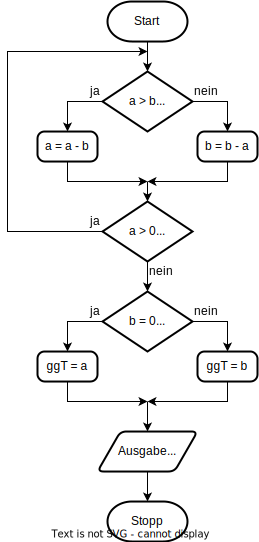
\includegraphics[scale=0.9]{Bilder/Kapitel-1/Abb-1-4.pdf}
    \vspace{\baselineskip} %%% für Druck
    \caption[Der Euklidische Algorithmus als Flussdiagramm]{Ein Flussdiagramm, das den Euklidischen Algorithmus zur Berechnung des größten gemeinsamen Teilers (ggT) zweier positiver Ganzzahlen grafisch darstellt}
    \label{fig:flussdiagramm}
\end{figure}

\pagebreak %%% für Druck

Den gleichen Zweck erfüllten die 1973 vorgestellten 
\marginline{Nassi-Shneiderman-Diagramm}
\textit{Nassi-Shneiderman-Diagramme}, die die Prinzipien der strukturierten Programmierung auf die Ebene des Softwareentwurfs übertrugen und den geplanten Programmablauf in einfachen Diagrammen als Kombinationen aus Sequenzen und Kontrollstrukturen darstellten.

\begin{figure}[h!]
	\centering
	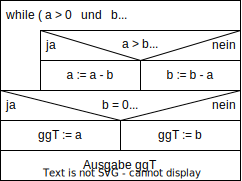
\includegraphics[scale=1.1]{Bilder/Kapitel-1/Abb-1-5.pdf}
	\caption{Der Euklidische Algorithmus als Nassi-Shneiderman-Diagramm}
	\label{fig:nassi_shneiderman_diagramm}
\end{figure}

1977 stellte Douglas Ross, auch ein Teilnehmer der 1968er-Konferenz, die \textit{\mbox{Structured} Analysis and Design Technique} (SADT) \marginline{SADT}
für den Entwurf von Softwaresystemen vor. SADT bildet die Funktionen der (zukünftigen) Software in Form einfacher hierarchischer Diagramme mit Angabe von Eingabe (engl. Input) und Ausgabe (engl. Output) sowie weiteren Informationen (\zb benötigte Ressourcen, äußere Einflüsse) ab. Die Diagramme können sowohl während der Anforderungsanalyse (\zb als Kommunikationsmittel mit dem Auftraggeber über die benötigten Funktionalitäten) als auch in der Entwurfsphase (\zb zur Aufteilung des Systems in Module) verwendet werden. Parallel dazu entwickelten Edward Yourdon und Larry Constantine seit Mitte der 1970er Jahre die Entwurfsmethode \textit{structured design} (SD). \marginline{SD, SA}
Sie selber und auch verschiedene andere Autorinnen und Autoren stellten in den Folgejahren sowohl weitere Varianten dieser Methode vor als auch mit \textit{structured analysis} (SA) Methoden für den Bereich der Anforderungsanalyse. 
 
Den Spezifikations- und Entwurfsmethoden der 1970er Jahre ist gemeinsam, dass die Funktionalitäten der Software nicht als Code einer konkreten Programmier\-sprache, sondern abstrakt als Pseudocode oder durch grafische Notationen (Diagramme) dargestellt werden. Dies führte dazu, dass ungenügend spezifizierte Anforderungen oder Schwachstellen in der Struktur der zukünftigen Software schon vor der Implementierung entdeckt werden konnten -- aber natürlich nicht zwangsläufig immer wurden. Die eigentliche Programmcodeerstellung konnte so systematischer ablaufen und wurde zudem besser planbar, da im Idealfall durch die vorgeschalteten Analyse- und Entwurfsprozesse die später zu implementierenden Funktionen schon feststanden. Die Übertragung der \textbf{Programmier}methoden der 1960er Jahre auf die höhere Abstraktionsebene von \textbf{Spezifikations-} und \textbf{Entwurfs}methoden der 1970er Jahre brachte die Professionalisierung der Softwareentwicklung einen großen Schritt voran.

\sttpDefinitionskasten{\sttpDefinitionskastenSkalierungsfaktor}{Implementierung}{Prozess der Programmcodeerstellung eines Softwareprodukts auf Basis einer in Nicht-Code formulierten Vorlage, wie zum Beispiel ein mathematisch oder allgemeinsprachlich definierter Algorithmus oder ein grafisch oder textuell beschriebener Softwareentwurf.}{In einer zweiten Bedeutung wird mit dem Begriff Implementierung (\textbf{die} Implementierung) häufig auch das Ergebnis der Implementierung, also der entstandene Programmcode bezeichnet. Im Rahmen dieses Textes verwenden wir den Begriff Implementierung in Abgrenzung zu den anderen Prozessen des Softwareengineering (\zb Prozess der Anforderungsermittlung) in seiner ersten Bedeutung.}

\minisec{Entwicklungen der 1980er Jahre}

Mit der Verbreitung der PC (Personal Computer) seit Anfang der 1980er Jahre nahm die Bedeutung von Softwareprodukten noch einmal stark zu. Die Softwarehersteller richteten ihren Blick jetzt auf den gesamten Lebenszyklus ihrer Produkte, von der Erfassung der (vermuteten) Kundenwünsche, über den Softwareentwurf, bis zu Implementierung und Test der Software, und noch weiter zur Wartung und Weiterentwicklung der Softwareprodukte. Gleichzeitig nahm die Anzahl der Entwicklungswerkzeuge für die Softwareentwicklung beständig zu. Schon seit Ende der 1960er Jahre waren im Zuge der strukturierten Programmierung erste Werkzeuge entstanden, die die Programmierer dabei unterstützen sollten, bei der Implementierung die Prinzipien dieser Programmiermethode anzuwenden. Aus heutiger Sicht kann man diese Werkzeuge als die ersten, noch sehr einfachen, \textit{CASE Tools} \marginline{CASE Tools}
(Computer-Aided Software Engineering Tools) bezeichnen. Die bisherigen Werkzeuge zur Unterstützung der Implementierungsarbeiten wurden jetzt in den 1980er Jahren durch solche ergänzt, die Aspekte der Anforderung und des Entwurfs unterstützten. Zudem entstanden die ersten Werkzeuge zum automatisierten Testen von Programmcode sowie Werkzeuge und Hilfen für das Projektmanagement von Softwareentwicklungsprojekten.

Schon seit den 1970er Jahre hatten die Softwarehersteller den Blick auch auf die organisatorisch geprägten Aktivitäten des Softwareentwicklungsprozesses gerichtet. So wurden Konzepte und Techniken der Planung, der Kostenabschätzung, der Steuerung und des Controllings aus dem klassischen Projektmanagement (und zunehmend auch deren Werkzeuge) für die Softwareentwicklung adaptiert. Je komplexer die Softwareentwicklungsprojekte wurden und je mehr Personen an der Erstellung einer Software beteiligt waren, desto stärker versuchte man auch, (gut funktionierende) Arbeitsprozesse auf spätere Projekte zu übertragen. Mit dem Wasserfallmodell und dem Spiralmodell verbreiteten sich so seit Mitte der 1980er Jahre die ersten 
\sttpkapitelverweis{Vorgehens\-modelle}{Kap.~\ref{sec:Kap-2}}
\textit{Vor\-gehens\-modelle} der Softwareentwicklung. Vorgehensmodelle organisieren die Tätigkeiten der Softwareentwicklung in logische Abschnitte und definieren die Übergänge zwischen diesen Abschnitten. Die ersten Vorgehensmodelle waren Phasenmodelle, in denen die Prozesse des Softwareengineering, wie zum Beispiel Anforderungen ermitteln, Softwareentwurf festlegen etc., anhand einer Zeitachse in aufeinanderfolgende Phasen eingeteilt wurden. Spätere Vorgehensmodelle sahen parallele Phasen oder wiederholte zyklische Abläufe der Prozesse vor. Heute werden verschiedene Arten von Vorgehensmodellen in der Softwareentwicklung eingesetzt. 

\minisec{Objektorientiertes Softwareengineering}

Auf der Implementierungsebene sind die späten 1980er Jahre durch das Aufkommen der \textit{objektorientierten Programmierung} geprägt. 
Erste objektorientierte Sprachen hatte es schon seit den 1960er (Simula-67) und 1970er (Smalltalk) Jahren gegeben, aber erst mit der Entwicklung von C$++$ und Objective-C hielten die Prinzipien der objektorientierten Programmierung wirklich Einzug in die Implementierung. Die heute weit verbreitete objektorientierte Sprache Java folgte Mitte der 1990er Jahren und trug viel dazu bei, dass sich die objektorientierte Programmierung so stark durchsetzte. Modularisierung, Geheimnisprinzip und vor allem Wiederverwendung von Programmkomponenten – ein schon auf der 1968er-Konferenz angesprochenes, aber damals kaum beachtetes Thema – sind wichtige Elemente dieses Programmierparadigmas. 

Mit der objektorientierten Programmierung erhielt auch der Bereich der Softwaretests 
%\sttpgls{Softwaretests}
einen höheren Stellenwert. Programmcode, der (evtl. auch vielfach und in verschiedenen Softwareprodukten) wiederverwendet werden soll, stellt höhere Ansprüche an die Qualität des Testprozesses. Aufgrund der starken Modularisierung ist das Testen zudem aufwändig, da sowohl die einzelnen Module als auch das Zusammenspiel der Module getestet werden müssen. Gleichzeitig verringern die Kapselung 
%\sttpgls{Kapselung}
und die definierten Schnittstellen der Module aber die Komplexität der einzelnen Tests und bieten die Möglichkeit, (Teile der) Tests zu automatisieren. 

Wie schon bei der strukturierten Programmierung folgten auf die objektorientierten \textbf{Programmier}methoden entsprechende objektorientierte \textbf{Entwurfs}methoden. Diese unterschieden sich teilweise sehr: Sie waren eng auf eine bestimmte Programmiersprache ausgerichtet, oder bezogen sich nur auf bestimmte Anwendungsgebiete, oder (zurück zu den Anfängen) waren nur für bestimmte Typen von Hardware gedacht. Allen Entwurfsmethoden war aber wieder gemeinsam, dass sie nicht mit Hilfe von Programmcode, sondern abstrakter kommuniziert wurden – im überwiegenden Fall durch Diagramme, teilweise ergänzt um formale textuelle Spezifikationen. Parallel zu den Entwurfsmethoden entwickelten sich Werkzeuge für die Unterstützung des objektorientierten Entwurfs- und Implementierungsprozesses. 

Bei aller Unterschiedlichkeit der objektorientierten Entwurfsmethoden im Detail bauten sie überwiegend auf der Idee auf, zu Beginn eines Softwareentwicklungsprojekts ein sogenanntes \textit{Domänenmodell} 
\marginline{Domänenmodell}
%\sttpkapitelverweis{Domänenmodell}{Kap.~\ref{sec:Kap-3.2.3}}
zu erstellen. Je nach Entwurfsmethode setzte sich dieses aus unterschiedlich vielen Diagrammen und textuellen Spezifikationen zusammen. Im Domänenmodell werden die für die zu entwickelnde Software relevanten Objekte des relevanten fachlichen Bereichs (die sogenannte Domäne), ihre Beziehungen zueinander sowie relevante Prozesse oder Aktivitäten der Domäne in einer auch für Nicht-Programmierer verständlichen Weise modelliert. Das Domänenmodell sollte im Laufe des Softwareentwicklungsprozesses schrittweise in immer detailliertere und in der Darstellungsform immer stärker auf die Implementierung ausgerichtete Modelle transformiert werden. Am Ende des Wegs sollte ein Modell stehen, das sich nach festen Regeln (und idealerweise sogar  automatisiert) in Programmcode umsetzen lässt. 

Die Vielfalt der objektorientierten Entwurfsmethoden erschwerte jedoch die Entwicklung von CASE Tools und die Kommunikation zwischen verschiedenen Softwareentwicklungsprojekten. Um eine vereinheitlichte Notation für die Spezifikation und den Entwurf von Softwaresystemen zu schaffen, arbeitete man in den 1990er Jahren – auf Basis der zu dieser Zeit verbreitetsten objektorientierten Notationen – an der Entwicklung der \textit{Unified Modeling Language (UML)}.
\marginline{UML} 
%\sttpkapitelverweis{UML}{Kap.~\ref{sec:Kap-3.2.2}}
Die Version 1.0 der UML wurde 1997 veröffentlicht. Seitdem hat sie zahlreiche kleinere Änderungen und Ergänzungen, aber auch umfassende Neustrukturierungen erfahren. Heute aktuell ist die Version 2.5.1, die Ende 2017 veröffentlicht wurde. Die UML stellt verschiedene Diagrammarten zur Verfügung, mit denen sich sowohl die Domäne selber als auch statische und dynamische Aspekte des zu entwickelnden Softwareprodukts modellieren lassen. Sie zeichnet sich dadurch aus, dass sie für unterschiedliche Domänen eingesetzt werden kann und (relativ) unabhängig ist von der Wahl des Vorgehensmodells für den Softwareentwicklungsprozess und von der konkreten objektorientierten Programmiersprache der Implementierung. Auf der UML bauen zahlreiche Entwicklungswerkzeuge auf. Das Spektrum reicht von Tools, die bei der Erstellung von UML-Diagrammen unterstützen bis zu solchen, die auf Grundlage von UML-Diagrammen Quellcode bestimmter Programmiersprachen erzeugen.

\minisec{Softwareengineering seit den 1990er Jahren}

Auf der Implementierungsebene entwickelten sich in den 1990er Jahren vermehrt Skriptsprachen. \marginline{Skriptsprachen}
Eine Skriptsprache ist eine Programmiersprache, die über einen Interpreter ausgeführt wird und nicht wie klassische höhere Programmiersprachen compiliert wird. Die frühen Skriptsprachen der 1970er und 1980er Jahre wurden meist nur für kleinere Automatisierungen (\zb einfache Shell- oder Batch-Skripte) verwendet, während Skriptsprachen wie Perl (1987), Python (1991) oder PHP (1995) auch für komplexere Aufgaben eingesetzt werden konnten. Die heute bekannteste Skriptsprache ist JavaScript, deren Version 1.0 im Jahr 1996 eingeführt wurde. Der verstärkte Einsatz von Skriptsprachen seit den 1990er Jahren ist eng verbunden mit der Einführung des World Wide Web (WWW) im Jahr 1991. Skriptsprachen wurden zunächst im WWW nur dafür verwendet dynamische Seiteninhalte in statische HTML-Seiten einzubinden, heute mittlerweile aber überwiegend zur Erstellung kompletter Webanwendungen. 

Das Aufkommen von Internet und WWW führte in den darauffolgenden Jahren und Jahrzehnten auch zu neuen Softwarekonzepten und -architekturen (\zb Client-Server Architekturen, Cloud Computing, Webservices, Software as a Service). Aus Soft\-ware\-engi\-neer\-ing-Sicht bedeutet das vor allem neue Herausforderungen 
\linebreak %%% für Druck
im Bereich Dezentralisierung (verteilte Software) und stark gestiegene Ansprüche im Bereich Wiederverwendung von Komponenten und Programmen. Mit der zunehmenden Verbreitung und Nutzung von anerkannten Entwurfsprinzipien, Entwurfs- und Architekturmustern sowie der stetigen Entwicklung und Verbesserung von 
\linebreak %%% für Druck
Bibliotheken und Frameworks hielt zudem eine ganz neue Ebene von Standardisierung und Wiederverwendbarkeit, aber auch von Abstraktion, Einzug ins Softwareengineering. 

Architektur- und Entwurfsmuster 
\marginline{Muster, Bibliotheken, Frameworks} 
sind abstrakt beschriebene Schablonen bewährter Lösungen für wiederkehrende und gleichartige Probleme, an denen man sich bei der Entwicklung seines eigenen Softwareprodukts orientieren kann. Bibliotheken bestehen aus Sammlungen mit Programmcodekomponenten, die nützliche und allgemeine Funktionalitäten zur Verfügung stellen, die aus dem eigenen Programmcode heraus aufgerufen werden können. Diese Funktionalitäten müssen Entwickler daher in ihrem eigenen Softwareprojekt nicht mehr selber programmieren, sondern nutzen die von anderen dafür erstellten Operationen. Frameworks gehen auf diesem Weg der Wiederverwendung noch einen Schritt weiter. Ein Framework liefert bereits das komplette Grundgerüst für ein Softwareprogramm. Die Entwickler müssen innerhalb dieses Grundgerüsts dann nur noch die Aspekte programmieren, die spezifisch für ihre Software sind, alles andere wird übernommen. Alle diese Konzepte fielen nicht in den 1990er Jahren plötzlich vom Himmel; viele Ursprünge, Vorarbeiten oder mindestens Ideen kann man bereits in den 1970er und 1980er Jahren finden. Erst jetzt setzte sich deren Nutzung aber verbreitet durch. Heute ist kaum ein komplexeres Softwareentwicklungsprojekt denkbar, das nicht in irgendeiner Weise auf Mustern, Bibliotheken oder Frameworks -- in der Regel sogar auf Kombinationen davon -- aufbaut.

\minisec{Weiterentwicklung und Standardisierung}

\sttpAutorenkasten{Grady Booch}{1955}{}{
	\vspace{4mm} %%% für Druck
	US-amerikanischer Informatiker. Entwickelte zusammen mit Ivar Jacobson und James Rumbaugh die UML und wurde dafür mit dem Computer Pioneer Award ausgezeichnet. Arbeitete viele Jahre bei Rational Software und war dort maßgeblich an der Entwicklung des Vorgehensmodells Rational Unified Process beteiligt.
	\vspace{4mm} %%% für Druck
}
{Bilder/Autoren/booch.jpg}{2013}{vonguard, \href{https://creativecommons.org/licenses/by-sa/2.0}{CC BY-SA 2.0}, via \href{https://commons.wikimedia.org/wiki/File:Grady_Booch,_CHM_2011_2_cropped.jpg}{Wikimedia Commons}}

Zum 50jährigen Jubiläum \marginline{Software\-engineering entwickelt sich stetig weiter} des Softwareengineering 2018 verfasste Grady Booch – einer der Pioniere der objektorientierten Softwareentwicklung und maßgeblich an der Entstehung der UML beteiligt – einen Überblicksartikel zur Geschichte des Softwareengineering \cite{boo18}. 
In diesem vertritt er die These, dass Softwareengineering über die Jahrzehnte immer auch in Reaktion auf äußere Zwänge gereift sei. Jede Zeitperiode der letzten fünfzig Jahre stellte anhand von technologischen (\zb verfügbare Hardware, Grad der Vernetzung von Computern), aber auch gesellschaftspolitischen Gegebenheiten (\zb Kalter Krieg, Globalisierung, Wandel der Arbeitswelt) ihre eigenen Anforderungen an Softwaresysteme und erzeugte so (explizit oder implizit) Druck auf das Feld des Softwareengineering, sich entsprechend weiterzuentwickeln. Durch die stetigen technologischen Fortschritte (Weiterentwicklung von Smart\-phones, Tablets etc., Internet of Things) entstanden und entstehen neue Arten von Softwaresystemen und damit wieder neue Herausforderungen für das Softwareengineering. Seit dem Aufkommen agiler Vorgehensmodelle verändern sich darüber hinaus auch Arbeitsprozesse in der Planung und organisatorischen Durchführung von Softwareprojekten.

Ob Softwareengineering eine (wissenschaftliche) Ingenieurdisziplin ist, oder immer noch auf dem Weg dorthin ist sich zu einer zu entwickeln, oder doch \textbf{nur} eine Sammlung von Best Practice Techniken darstellt, oder irgendetwas dazwischen ist, ist eine seit den Anfängen des Softwareengineering wiederholt geführte, kontroverse Diskussion.\footnote{Zusammenfassende Überblicke zu dieser Diskussion finden sich insbesondere bei \cite{dia14}, \cite{mah04}, \cite{gri11}. Wer sich noch intensiver mit dem Thema Softwareengineering als Disziplin befassen möchte, sei zusätzlich auf \cite{sei14} und \cite{wan00} verwiesen.} 
In jedem Fall haben sich über die Jahre verschiedene Merkmale einer Disziplin, wie (Sektionen von) Fachgesellschaften und Berufsverbänden, Gremien, Fachzeitschriften, Curricula, Handbücher und Standards für den Bereich des Softwareengineering herausgebildet. 

\phantomsection
\label{text:Sevocab}
Im Jahr 1983 veröffentlichte das Institute of Electrical and Electronics Engineers (IEEE, \href{https://www.ieee.org/}{www.ieee.org})\footnote{Das IEEE betreibt eine eigene Online-Bibliothek, in der die Artikel der eigenen Fachzeitschriften, Konferenzpublikationen und Standardisierungsdokumente gelistet sind (\href{https://ieeexplore.ieee.org}{https:
		\linebreak %%% für Druck
		//ieeexplore.ieee.org}). Aus dem Netz der FernUniversität besteht kostenloser Zugriff auf die Volltextversionen vieler gelisteter Einträge.} -- ein seit 1963 existierender weltweiter Berufsverband von Ingenieuren, der auch als Standardisierungsgremium agiert -- zum ersten Mal ein Glossar für den Bereich des Softwareengineering. Auf diesem Standard und seiner Nachfolgeversion von 1990 aufbauend entstand in gemeinsamer Arbeit zwischen IEEE und ISO/IEC (Normungsinstitutionen) in den 2000er Jahren die
\marginline{SEVOCAB} 
\textit{SEVOCAB}-Datenbank, mit dem Ziel, in der Profession eine standardisierte Terminologie, ein gemeinsames Begriffs\textbf{verständnis} und eine einheitliche Begriffs\textbf{verwendung} zu etablieren. SEVOCAB steht für „systems and software engineering vocabulary“. Wie der Name schon sagt, finden sich in SEVOCAB Begriffserläuterungen für Begriffe aus dem Bereich des Softwareengineering und des Systems Engineering.\footnote{Systems Engineering beschäftigt sich mit dem gesamten Lebenszyklus und allen Aspekten komplexer technischer Systeme (Hardware und Software, Verfahren und Prozesse, Einbettung in das Anwendungsumfeld).} Die in SEVOCAB enthaltenen Definitionen wurden größtenteils nicht neu entwickelt, sondern aus etablierten Normen und Standards verschiedener Standardisierungs\-gremien dieses Bereichs übernommen. Dadurch finden sich in SEVOCAB auch mehrere, gleichwertig nebeneinander stehende, unterschiedliche Definitionen einzelner Begriffe, jeweils mit Verweis auf den zugrundeliegenden Standard. Eigene Defini\-tionen nimmt SEVOCAB nur an Stellen vor, an denen Bedeutungen aus verschiedenen Standards zu widersprüchlich sind. Neue Entwicklungen im Bereich Systems Engineering und Softwareengineering werden berücksichtigt, indem Definitionen aus abgelösten Standards entfernt und die der neuen Standards hinzugefügt werden. 

\sttpHinweiskasten{1.0}{abgelöste Standards}{Standards, die nicht mehr aktuell sind, werden von den jeweiligen Standardisierungsgremien als „withdrawn“ (zurückgezogen) oder „superseded“ (ersetzt, abgelöst) markiert, um Nutzern zu sig\-na\-li\-sie\-ren, welche Standards noch Gültigkeit haben und welche nicht.}

In regelmäßigen zeitlichen Abständen wird die zum jeweiligen Zeitpunkt bestehende Datenbasis von SEVOCAB als ISO/IEC Norm veröffentlicht. Die online frei verfügbare SEVOCAB-Datenbank (\href{http://www.computer.org/sevocab}{www.computer.org/sevocab}) wird kontinuierlich erweitert, ist in der Regel also aktueller als die letzte veröffentlichte Norm, besitzt nur nicht deren rechtlich akzeptierten Status.

\phantomsection
\label{text:SWEBOK}
Aufbauend auf vorhandenen Standards 
\marginline{SWEBOK - Kompendium des Software\-engineering}
arbeiteten internationale Softwareingenieure unter Führung des IEEE seit Ende der 1990er Jahre daran, ein Kompendium des Softwareengineering zu erstellen. Ziel ist es, den Kern des allgemein akzeptierten, in der Praxis verwendeten und als wesentlich identifizierten Wissens („core body of knowledge“) für das Berufsfeld des Softwareengineering – auch im Hinblick auf Ausbildung und Fortbildung – zu strukturieren und zugänglich zu machen. Ausdrücklich nicht berücksichtigt werden sollten das Expertenwissen kleinerer Gruppen sowie laufende Forschungsfragestellungen. Ergebnis des (aufgrund intensiver Reviewverfahren) mehrjährigen Prozesses ist der 2004 erstmals erschienene „Guide to the Software Engineering Body of Knowledge“ (\textit{SWEBOK}). 
%\sttpMarginPicture{Bilder/Kapitel-1/Buchcover-SWEBOK.jpg}
Die aktuelle Version SWEBOK V3.0 aus dem Jahr 2014 \cite{swe14} kann nach einer Registrierung kostenlos von der Website der IEEE Computer Society heruntergeladen werden (\href{http://www.computer.org/web/swebok}{www.computer.org/web/swebok}). Aktuell wird an der Version 4.0 gearbeitet. 

SWEBOK teilt das Themenfeld Softwareengineering in fünfzehn Wissensgebiete („knowledge areas“) ein. Dazu gehören neben konkreten Prozessen der Softwareentwicklung wie Anforderungsanalyse und Softwareentwurf auch übergreifende Themen wie Soft\-ware\-qua\-li\-tät sowie notwendige Basis-Wissensgebiete wie Mathematische Grundlagen des Softwareengineering. 

Jedes Wissensgebiet wird kompakt auf fünfzehn bis zwanzig Seiten dargestellt. Dabei geht es weniger darum, konkretes Faktenwissen zu vermitteln, sondern darum, auf einer höheren Abstraktionsebene (hierarchische) Beziehungen, Überschneidungen und Abgrenzungen zwischen einzelnen Themen des Softwareengineering darzustellen. So beschäftigt sich zum Beispiel das Unterkapitel zu Vorgehensmodellen inhaltlich gar nicht mit den zwei wichtigen Vertretern Wasserfallmodell und Scrum, sondern erläutert, welche Kategorien von Vorgehensmodellen im Softwareengineering eingesetzt werden und nach welchen Kriterien sie sich voneinander abgrenzen lassen. 

Die Autorinnen und Autoren von SWEBOK haben zudem sehr darauf geachtet, jedes Kapitel – ein Kapitel entspricht einem Wissensgebiet – einheitlich zu gliedern und Beziehungen zwischen den Wissensgebieten deutlich herauszustellen. Die für SWEBOK verwendete Art der Strukturierung hat den Vorteil, dass das präsentierte Wissen weniger schnell veraltet. Zudem bietet sie einen stark analytischen Zugang zum Feld des Softwareengineering. Für Anfänger im Softwareengineering nachteilig kann aber der hohe Abstraktionsgrad der Texte sein. Daher werden für die fakten\-orien\-tier\-tere Beschäftigung mit den Themen in allen Unterkapiteln Verweise auf konkrete Kapitel und sogar einzelne Seiten von Lehrbüchern angegeben, die die Autorinnen und Autoren des SWEBOK als Standardliteratur zum entsprechenden Gebiet identifiziert haben. 

% 1.2
\clearpage
\section{Softwareengineering heute}
\label{sec:Kap-1.2}
% Für diesen Abschnitt ist kein Text vorgesehen.
\subsection{Was ist Softwareengineering?}
\label{sec:Kap-1.2.1}

Softwareengineering wurde erstmalig bedeutsam, als Software breitentauglicher (Einsatz auch außerhalb von Forschungseinrichtungen) werden sollte und gleichzeitig die Einsatzfelder von Software zu kritisch waren (\zb Verteidigungssysteme, medizinische Geräte), als dass man „ungeplant“ hätte entwickeln können. Aus den bisherigen Darstellungen sollte deutlich geworden sein, dass es im Laufe der letzten Jahrzehnte sich verändernde, ergänzende, aber teilweise auch konkurrierende Vorstellungen gab, welche Aspekte Softwareengineering beinhalten und in welche Richtung es sich weiterentwickeln soll. Wenn man heute in Lehrbüchern nach Definitionen zum Softwareengineering sucht, findet man -- trotz Standardisierungsbemühungen wie den Arbeiten an SWEBOK -- immer noch viele verschiedene Vorschläge. Zum einen unterscheiden sie sich darin, welche Prozesse aus dem Bereich der Erstellung von Software dem Softwareengineering zugerechnet werden und welche nicht: Gehören beispielsweise die Kostenkalkulation des Softwareprojekts, die Zusammenstellung des Entwicklerteams oder die Wahl des Vorgehensmodells schon in den Bereich Softwareengineering oder beginnt Softwareengineering erst \textbf{danach}? Wann endet Softwareengineering: Inwiefern gehören Wartung, Weiterentwicklung, aber auch Vertrieb der Software dazu? Zum anderen gehen die Meinungen, inwieweit Softwareengineering eine (echte) ingenieurwissenschaftliche Disziplin ist, auch heute noch auseinander (dasselbe gilt im Übrigen auch für die gesamte Informatik). Die Gründe für die unterschiedlichen Vorstellungen über das Gebiet Softwareengineering sind die gleichen wie vor fünfzig Jahren: Menschen mit unterschiedlichen (beruflichen) Hintergründen oder unterschiedlichen aktuellen Arbeitsgebieten definieren Softwareengineering und vor allem auch das Aufgabengebiet von Softwareingenieuren und -ingenieurinnen unterschiedlich.

Nichtsdestotrotz
\marginline{Prinzipien des Ingenieur\-wesens für die Entwicklung von Software nutzen} 
besteht heute Einigkeit darüber, dass Softwareengineering sich dadurch auszeichnet, dass Prinzipien des Ingenieurwesens auf die Entwicklung von Software angewendet werden. Dazu gehören die systematische Entwicklung und Verwendung von Methoden, Standards und Werkzeugen und die Entwicklung von Maßsystemen zur Messung und Qualitätsbeurteilung von Softwareeigenschaften genauso wie die intensive Nutzung von Erfahrungswerten.

Des Weiteren sind folgende Punkte Konsens: 
\begin{itemize}
	\item Softwareengineering ist mehr als nur Programmierung, beinhaltet also noch weitere Prozesse.
	\item Softwareengineering beschäftigt sich mit der \textbf{systematischen} Entwicklung von \textbf{komplexer} Software. Es geht also zum einen darum, geplant zu entwickeln, statt „irgendwie zu programmieren“. Und zum anderen liegt der Fokus auf den größeren, komplexeren Softwaresystemen und nicht auf dem kleinen, einfachen Programm zur automatischen Bewässerung der eigenen Zimmerpflanzen.
	\item Softwareengineering beruht neben theoretischen (mathematischen) Grund\-lagen auch auf heuristischen Techniken und Methoden (Best Practices).
\end{itemize}

\pagebreak %%% für Druck

Der schon erwähnte SEVOCAB-Standard definiert Softwareengineering dementsprechend als: 

\sttpzitat{„systematic
\marginline{Definition\\Software\-engineering} 
application of scientific and technological knowledge, methods, and experience to the design, implementation, testing, and documentation of software.”}{Eintrag „software engineering“ bei \href{http://www.computer.org/sevocab}{www.computer.org/sevocab}}

\vspace{\baselineskip} %%% für Druck

Die SEVOCAB Softwareengineering-Definition stellt die theoretisch fundierten Erkenntnisse und die Erkenntnisse aus praktischen Erfahrungen gleichwertig neben\-einander. Wie Sie im Laufe des Textes noch lesen werden, dominieren aber in manchen Prozessen des Softwareengineering – vor allem in der Anforderungsermittlung und im Entwurf – heute die Best Practice Techniken. Eine theoriegeleitete Beschäftigung mit Softwareengineering existiert nichtsdestotrotz auch heute noch, und dies hat auch eine starke Berechtigung. Einerseits werden hier Grundlagen entwickelt, die in der Zukunft die Softwareentwicklung revolutionieren könnten. Zum Anderen unterscheiden sich Softwaresysteme unter anderem darin, welche Konsequenzen Fehler haben. Stark sicherheitskritische Anwendungen, zum Beispiel in der Raumfahrt oder in der Medizintechnik, erfordern ein weit höheres Maß an Vertrauen in die Korrektheit von Software als andere Anwendungen; hier spielen formale Methoden weiterhin eine große Rolle.

\vspace{\baselineskip} %%% für Druck

\phantomsection
\label{text:theoVertreter}

\sttpKastenBreakable{\textbf{formale Methoden vs. Best Practices}

Schon lange vor der Entstehung von agilen Entwicklungsansätzen, die in den 1990er Jahren eine bis heute bestehende Konfliktlinie zwischen Befürwortern und Gegnern agiler Softwareentwicklung eröffneten (s. Kap.~\ref{sec:Kap-2.3}), existierte im Softwareengineering eine ältere Konfliktlinie zwischen zwei wettstreitenden Fraktionen: diejenigen, die an formale Methoden und Korrektheitsbeweise für Software glaubten, und diejenigen, die all diese mathematisch-logisch orientierten Methoden für nicht praktikabel und viel zu aufwändig hielten. Beide Seiten hielten sich gegenseitig mangelhaftes ingenieurmäßiges Denken vor: Die formale Fraktion verwies auf die formalen Grundlagen in den anderen Ingenieurwissenschaften (\zb Statikberechnungen), die andere Seite verwies auf die Orientierung an Best Pratices und die Notwendigkeit, Methoden für aktuell existierende Probleme und aktuelle Softwareentwicklungsprojekte zu erstellen, statt Grundlagen für irgendeine Zukunft zu legen. Formale Spezifikationen zu Projektbeginn bei der Formulierung von Anforderungen können in diesem Zusammenhang als ein Kompromiss betrachtet werden. Die Vision der formalen Fraktion war und ist, dass Software eigentlich gar nicht mehr (von Menschen) entwickelt werden muss, sondern automatisch aus hinreichend präzisen Anforderungen generiert wird und dann per Konstruktion diese Anforderungen erfüllt (natürlich muss dafür auch diese Generierungssoftware fehlerfrei sein). Mit diesem Ziel wurden und werden eigene Sprachen für die Spezifikation und auch neue Programmiersprachen entwickelt. Man könnte diese Forschungsrichtungen ebenfalls Softwareengineering nennen, tatsächlich verteilen sie sich aber über andere Teildisziplinen der Informatik, und werden auch an der FernUniversität in anderen Modulen gelehrt. Deshalb gehen wir auch in diesem Text den sehr formalen Ansätzen nicht intensiver nach. Bemerkenswert bleibt aber, dass die Ursprünge des Softwareengineering durchaus auch auf eher formalen Ansätzen beruhten und beide genannten Fraktionen anfangs beteiligt waren.}

\vspace{\baselineskip} %%% für Druck

Softwareengineering ist ein Fachgebiet, das sich weiterhin im Wandel befindet. Anhand der Herausforderungen neuer Softwarekonzepte oder neuer Arten von Soft\-ware\-syste\-men entstehen neue, erweiterte oder veränderte Programmiersprachen, Notationen, Vorgehensmodelle, Methoden und Techniken in allen Bereichen des Soft\-ware\-lebens\-zyklus - und das meist außerhalb des wissenschaftlichen Bereichs. Jenseits aller Standardisierungsbemühungen und verschiedener Versuche, der Disziplin ein stärkeres wissenschaftliches Fundament zu geben, wird sich Softwareengineering auch weiterhin in erster Linie dadurch definieren, welche Fähigkeiten ein Soft\-ware\-inge\-nieur in der Praxis benötigt und was er in seiner täglichen Arbeit tut. Die universitäre Lehre (und einen Lerntext zum Thema Softwareengineering) stellt dies vor große Herausforderungen. Wenn wir uns zu sehr auf die neuesten oder aktuell beliebtesten Entwurfsmethoden, Frameworks oder Entwicklungswerkzeuge konzentrieren, könnte das, was wir heute als neueste Errungenschaften lehren, morgen schon wieder veraltet sein. Es könnte sich auf der anderen Seite in der Praxis (noch) nicht durchgesetzt haben bzw. sich nie durchsetzen. Um das beliebte Beispiel der Vorgehensmodelle noch einmal zu bemühen: Wir können sowohl Scrum als auch das Wasserfallmodel vorstellen (und werden das auch tun), aber aus Lehrperspektive wichtiger ist die Vermittlung, was ein Vorgehensmodell auszeichnet, warum man es im Softwareengineering einsetzt und welche Vor- und Nachteile unterschiedliche Kategorien von Vorgehensmodellen haben.

Heute gibt es sehr viele unterschiedliche Arten von Softwaresystemen, für die unterschiedliche Softwareengineering-Techniken erforderlich sind. So werden sich das Softwareengineering für eine stand-alone Fotobearbeitungssoftware, für ein eingebettetes System eines Autos und für eine Webanwendung eines Onlineshops in den eingesetzten Programmiersprachen, Vorgehensmodellen und Entwurfstechniken stark unterscheiden.
\marginline{die grundlegenden Aspekte des Software\-engineering} 
Die unterliegenden Ideen und Konzepte des Softwareengineering lassen sich aber für alle Softwaresysteme anwenden: Für jede industriell gefertigte Software müssen in irgendeiner Art und Weise Anforderungen spezifiziert werden, die in irgendeiner Notation dokumentiert werden müssen. Jede Software durchläuft irgend\-wann einen oder mehrere Entwurfsprozess(e), muss implementiert, verifiziert oder getestet, an die Kunden ausgeliefert und gewartet werden. Und alle diese Aktivitäten müssen innerhalb gegebener Zeit-, Kosten- und Personalbudgets in hoher Qualität erfolgreich abgeschlossen werden. Dementsprechend beschäftigt sich dieser Text schwerpunktmäßig mit den grundlegenden Aspekten des Softwareengineering, die unabhängig von der Art des zu entwickelnden Softwaresystems eine Bedeutung haben.

\clearpage %%% für Druck
\subsection[Rollen, Prozesse, Aktivitäten – Begriffe des Software-\\engineering]{Rollen, Prozesse, Aktivitäten – Begriffe des Softwareengineering}
\label{sec:Kap-1.2.2}

An einem Softwareentwicklungsprojekt sind in der Regel verschiedene Personengruppen beteiligt, die im Englischen und mittlerweile zunehmend häufiger auch in deutschsprachiger Literatur mit dem Begriff \textit{Stakeholder} \marginline{Stakeholder} 
(Interessenvertreter) bezeichnet werden. Zu den Stakeholdern eines Softwareentwicklungsprojekts zählen zum Beispiel Softwareentwickler, Softwarearchitekten, Tester, Qualitätssicherungsexperten, Projektleiter, Domänenexperten, Auftraggeber, (zukünftige) Nutzer. 

Je nach Projektgröße werden unterschiedlich viele Personen am Projekt beteiligt sein. Gerade bei kleineren Projekten muss ein konkretes Teammitglied oft mehrere Aufgaben wahrnehmen, zum Beispiel könnten die Aufgaben der Soft\-ware\-archi\-tektin 
%\sttpgls{Softwarearchitekt}
von einer der Softwareentwicklerinnen mit übernommen werden oder der Auftraggeber gleichzeitig der Domänenexperte 
%\sttpgls{Domaenenexperte}
sein. In großen Projekten könnten mehrere Teammitglieder identische oder ähnliche Aufgabengebiete besitzen oder ein Aufgabengebiet von wechselnden Personen übernommen werden. Wenn man über das Team spricht, das an einem Softwareentwicklungsprojekt beteiligt ist, abstrahiert man daher von konkreten Personen und spricht stattdessen von sogenannten Rollen. Jeder Rolle sind bestimmte Aufgaben zugeordnet. Zudem ist sie mit spezifischen Kenntnissen und Fähigkeiten verknüpft, die benötigt werden, um die der Rolle zugeordneten Aufgaben ausführen zu können. Im konkreten Projekt nimmt jedes Teammitglied eine oder mehrere Rollen ein und führt die der Rolle/den Rollen zugeordneten Tätigkeiten aus.

\sttpDefinitionskasten{\sttpDefinitionskastenSkalierungsfaktor}{Rolle im Softwareentwicklungsprojekt}{Abstrakte Beschreibung einer anonymen Person mit definierten Aufgaben und Befugnissen und entsprechenden Kenntnissen und Fähigkeiten.}{Das Konzept der Rolle ist im Softwareengineering mit mehreren Bedeutungen verbunden. In diesem Zusammenhang geht es um die Beschreibung von Akteuren im Rahmen der Softwareentwicklung.}

Die innerhalb eines Softwareentwicklungsprojekts durchgeführten einzelnen Tätigkeiten (\zb das Lastenheft schreiben, den Testplan erstellen, eine bestimmte Funk\-tion implementieren) kann man verschiedenen großen Bereichen des Soft\-ware\-entwick\-lungs\-prozesses zuordnen, wie zum Beispiel dem Bereich der Implementierung oder dem Bereich des Testens. Diese Teilbereiche des Softwareentwicklungsprozesses bezeichnen wir als \textit{Prozesse}. 

\begin{figure}[h!]
	\centering
	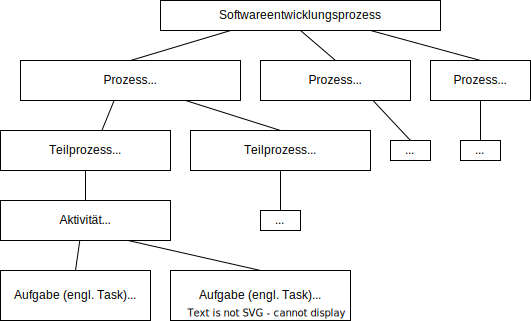
\includegraphics[scale=1.0]{Bilder/Kapitel-1/Abb-1-6.pdf}
	\caption{Zusammenhang zwischen Prozessen, Aktivitäten und Aufgaben}
	\label{fig:prozesse_aktivitaeten_aufgaben}
\end{figure}

Abbildung~\ref{fig:prozesse_aktivitaeten_aufgaben} zeigt den Zusammenhang \marginline{Prozess, Aktivität, Aufgabe} der in diesem Text verwendeten Begriffe: Ein Prozess, wie zum Beispiel der Prozess der Anforderungsermittlung, kann in \mbox{\textit{Teilprozesse}} weiter unterteilt werden. Jeder Teilprozess besteht aus einer Menge von \textit{Aktivitäten}, wie zum Beispiel „Lastenheft erstellen“ oder „Module der Software bestimmen“. Aktivitäten wiederum können in noch kleinere Einheiten, sogenannte \textit{Aufgaben} (engl. Tasks), unterteilt werden, die schlussendlich von Rollen ausgeführt werden. Ein konkreter Softwareentwicklungsprozess ist somit eine Menge aus einzelnen Aktivitäten zusammengesetzter Prozesse. Dabei können sich die Prozesse oder Teilprozesse auch überschneiden, sodass es häufig nicht möglich ist genau zu bestimmen, an welcher Stelle ein Prozess bzw. Teilprozess endet und ein anderer beginnt. Ebenso lässt sich nicht immer eindeutig bestimmen, welchem Teilprozess eine konkrete Aufgabe zugeordnet ist. 

Der Software Engineering Body of Knowledge (SWEBOK) definiert einen ingenieurwissenschaftlichen Prozess als

\sttpzitat{„a set of interrelated activities that transform one or more inputs into outputs while consuming resources to accomplish the transformation“. \cite[8-1]{swe14}}{}

Bezogen auf den Gesamtprozess der Entwicklung eines Softwareprodukts besteht der Input aus der Menge der Anforderungen an die zu erstellende Software und der Output aus dem fertigen Softwareprodukt. Die einzelnen Prozesse innerhalb des Softwareentwicklungsprozesses transformieren unterschiedliche Arten von Inputs in Outputs, wobei die Outputs eines Prozesses oft die Inputs eines oder mehrerer Folgeprozesse sind. So könnte zum Beispiel der Output eines Implementierungsprozesses ein Stück Programmcode sein und Letzteres ein Teil des Inputs für den Prozess des Testens. Bei den verbrauchten Ressourcen für die Erstellung des Softwareprodukts handelt es sich in erster Linie um die Arbeitszeit der an der Entwicklung beteiligten Personen. Ressourcen können aber zusätzlich auch Softwareressourcen (\zb fertige Softwarekomponenten, die in das Produkt eingebunden werden, oder für die Entwicklung verwendete Tools) und Hardwareressourcen (\zb Entwicklungsinfrastruktur) sein. 

\sttpHinweiskasten{1.0}{unterschiedliche Begriffsverwendung}{Beachten Sie, dass Teile der Literatur die großen Bereiche des Software\-entwicklungsprozesses wie Anforderungsermittlung/-analyse, Implementierung oder Testen nicht als \textbf{Prozesse}, sondern schon als \textbf{Aktivitäten} bezeichnen. Für konkrete Tätigkeiten, wie zum Beispiel für die Tätigkeit „das Lastenheft erstellen“ innerhalb der Anforderungs\-ermitt\-lung/-analyse werden dann Begriffe wie Unteraktivitäten oder Sub-Aktivitäten verwendet.}

Bei den angesprochenen Prozessen 
\marginline{Kernprozesse, unterstützende Prozesse}
des Softwareengineering unterscheidet man \textit{Kernprozesse} (engl. primary processes, development processes, implementation processes) von \textit{unterstützenden Prozessen} (engl. support processes). Letztere werden häufig auch als Softwaremanagementprozesse bezeichnet. Seit Mitte der 1980er Jahre besteht relative Einigkeit darüber, welche \textbf{Kernprozesse} dem Softwareengineering zuzurechnen sind, auch wenn die Benennungen, die konkreten Aktivitäten und die Abgrenzungen zwischen den Prozessen je nach Blickwinkel differieren können. Die Kernprozesse des Softwareengineering sind:
\begin{itemize}
	\item die Anforderungsermittlung/-analyse
	\item der Softwareentwurf
	\item die Implementierung
	\item das Testen bzw. allgemeiner die Qualitätssicherung sowie
	\item die Wartung, ggf. ergänzt um die Weiterentwicklung der Software
\end{itemize}

Mittlerweile ist unbestritten, dass neben den Kernprozessen auch Softwaremanagementprozesse Teil des Softwareengineering sind. Welche Managementprozesse dies genau betrifft, variiert aber stark in der Literatur. Der Schwerpunkt unserer Lehrveranstaltung liegt auf den Kernprozessen des Softwareengineering. 

\minisec{Aufbau des Textes}

Lassen Sie uns an dieser Stelle die inhaltliche Ebene kurz verlassen und auf die noch ausstehende Darstellung zum Aufbau des Textes zurückkommen. Kapitel~\ref{sec:Kap-2} in dieser ersten Lektion behandelt das Thema der Vorgehensmodelle und deren Zusammenhang zu den Prozessen des Softwareengineering. Die detaillierte Beschäftigung mit den eben vorgestellten Kernprozessen des Softwareengineering beginnt ab Lektion 4. Zuvor werden sich die Lektionen 2 und 3 allgemeiner mit dem Thema Modellierung beschäftigen, das in allen Prozessen des Softwareengineering eine Rolle spielt. Wie erwähnt legt der Text den Schwerpunkt auf grundlegende Aspekte des Softwareengineering, die weitestgehend unabhängig von der Art des (zu entwickelnden) Softwareprodukts sind. Einige andere Einschränkungen müssen wir aber treffen, um den Umfang im Rahmen zu halten: Die Lehrveranstaltung beschäftigt sich nur mit objektorientierter Softwareentwicklung und aus der Menge der möglichen Notationssprachen wird die Unified Modeling Language (UML) gewählt, die die bei Weitem größte Verbreitung genießt.  

% 1.3
% Kommentierte Literatur beginnt auf neuer Seite
\clearpage
\section{Kommentierte Literatur}
\label{sec:Kap-1.3}

%Bilder/Buchcover/Buchcover_Naur_Randell.png
\sttpKommLitItem{Naur/Randell}{1969}{Software Engineering: Report on a Conference 1968}{nau69}{}{}
{Der Abschlussbericht zur Softwareengineering-Konferenz in Garmisch 1968. Die Diskussionen auf der Konferenz wurden detailliert protokolliert und zu großen Teilen sogar auf Band aufgenommen, sodass der Bericht neben der Zusammenfassung des Dis\-kussions\-verlaufs auch Originalredebeiträge der Teilnehmer aus den Diskussionen darstellen kann. Eine redaktionelle Bearbeitung durch die Herausgeber des Berichts erfolgte dabei nur insofern, dass die Redebeiträge unabhängig von ihrer chronologischen Reihenfolge thematisch zugeordnet sowie inhaltlich passende Passagen aus den auf der Konferenz vorgestellten Working Papers der Darstellung des Dis\-kus\-sions\-verlaufs hinzugefügt wurden. Zur Folgekonferenz in Rom im Jahr 1969 existiert ebenfalls ein Abschlussbericht \cite{bux70}.}

%{Bilder/Buchcover/Buchcover_Laplante.jpg}{S. 1119-1126}
\sttpKommLitItem{Grier}{2011}{Software Engineering: History}{gri11}{}{}
{Sechsseitiger überblicksartiger Artikel zur Geschichte des Softwareengineering aus der Enzyklopädie des Softwareengineering \cite{lap11} unter dem Blickwinkel, durch welche Entwicklungen sich Softwareengineering zu einer eigenen Disziplin entwickelt hat. Die Meilensteine der sehr frühen Jahre werden chronologisch dargestellt. In der Folge beleuchtet der Artikel dann systematisch, welche Entwicklungen seit den 1970er Jahren bis Ende der 1980er Jahre bezüglich der Prozesse Spezifikation, Entwurf, Implementierung, Test und Wartung von Software wichtig waren. Abschließend beschäftigt sich der Artikel mit der Frage, welche der Merkmale einer Disziplin (Fachgesellschaften, Curricula, Handbücher etc.) Softwareengineering in der Gegenwart (2011) aufweist und inwiefern sich Softwareengineering von den klassischen Ingenieurwissenschaften unterscheidet.}

%{Bilder/Buchcover/Buchcover_Gonzalez.jpg}{72-1 bis 72–20}
\sttpKommLitItem{Díaz-Herrera/Freeman}{2014}{Discipline of Software Engineering: An Overview}{dia14}{}{}
{Ein umfangreicher Artikel aus dem Handbuch Computer Science and Software \linebreak %%% für Druck
	Engineering \cite{gon14}, der einen sehr detaillierten Überblick über die wichtigen Entwicklungen im Softwareengineering von den Anfängen bis zur Gegenwart (2014) gibt. Der Artikel verweist dabei auch intensiv auf die historischen Dokumente zur Softwareentwicklung (wie \zb die Arbeiten von Dijkstra und Parnas). Er ist daher sehr gut als Ausgangspunkt geeignet, um sich noch intensiver in die Geschichte des Softwareengineering zu vertiefen. Der Artikel stellt außerdem die Diskussion vor, ob und inwiefern Softwareengineering eine Disziplin ist.}

%Bilder/Buchcover/zeitung.png
\sttpKommLitItem{Booch}{2018}{The History of Software Engineering}{boo18}{}{}
{Inhaltlich sehr dichter (Aufzählung vieler Personen und Ereignisse) siebenseitiger Artikel zum 50jährigen Jubiläum des Softwareengineering über dessen Entwicklung, geschrieben von einem der Pioniere der objektorientierten Softwareentwicklung und der UML. Im Gegensatz zu der anderen hier vorgestellten Literatur beschäftigt sich der Artikel auch mit frühen Ereignissen der Computerhistorie des späten 19. und frühen 20. Jahrhundert (Babbage, ENIAC, Turing etc.). Zudem listet er Errungenschaften des Softwareengineering ab den späten 1990er Jahren auf, was die anderen hier vorgestellten Artikel zur Geschichte des Softwareengineering aufgrund ihrer Fokussierung auf die Disziplinfrage etwas vernachlässigen. Der Fokus des Artikels liegt dabei immer auf der Darstellung von technologischen und gesellschaftspolitischen Gegebenheiten der jeweiligen Jahrzehnte und deren Auswirkungen auf die Ausrichtung des Softwareengineering.}

%Bilder/Buchcover/zeitung.png
\sttpKommLitItem{del Águila/Palma/Túnez}{2014}{Milestones in Software Engineering and Know\-ledge Engineering History: A Comparative Review}{del14}{}{}
{Der Zeitschriftenartikel vergleicht die Meilensteine in der Entwicklung des Softwareengineering mit denen in der Entwicklung des Knowledge Engineering\footnote{in Deutsch: Wissensmodellierung. Das Themenfeld Knowledge Engineering in der Informatik beschäftigt sich mit der Erforschung und Entwicklung wissensbasierter Systeme. Es ist ein Teilgebiet des Bereichs künstliche Intelligenz.}. Für die Darstellung der Entwicklungen im Softwareengineering verwenden die Autorinnen und Autoren eine Kategorisierung von \cite{end97} aus dem Jahr 1996, die die Geschichte des Softwareengineering in wenige große zeitliche Phasen einteilt, und erweitern diese bis in die Gegenwart (2014). Dadurch zeigt der Artikel stärker als die bisher erwähnte Literatur die größeren Linien in der Geschichte des Softwareengineering, ist gleichzeitig aber auch deutlich weniger detailliert bezüglich der einzelnen Errungenschaften. Der eigentliche Fokus des Artikels liegt auf der Frage, wie Softwareengineering und Knowledge Engineering voneinander lernen und sich weiterentwickeln können.}

%Bilder/Buchcover/zeitung.png
\sttpKommLitItem{Mahoney}{2004}{Finding a History for Software Engineering}{mah04}{}{}
{Ein etwas anderer Ansatz die Entwicklung des Softwareengineering darzustellen. Der Wissenschaftshistoriker Michael Mahoney beleuchtet in seinem Zeitschriftenartikel die akademische und berufliche Sozialisation der Teilnehmer der 1968er-Konferenz, um zu erklären, warum es auf der Konferenz und auch bis in die Gegenwart (2004) so unterschiedliche Ansichten darüber gibt, in welche Richtung sich Softwareengineering entwickeln soll. Er identifiziert drei Gruppen [s. S.~\pageref{text:Mahoney}]. Im Rahmen der Vorstellung dieser drei Gruppen führt der Artikel wichtige Meilensteine der Entwicklung des Softwareengineering auf.}

%Bilder/Buchcover/Buchcover_Tanenbaum_Austin.jpg
\sttpKommLitItem{Tanenbaum/Austin}{2014}{Rechnerarchitektur: Von der digitalen Logik zum \\ %%% für Druck
	Parallelrechner}{tan14}{}{}
{Ein auch für Anfänger sehr gut verständliches Lehrbuch mit umfangreichen Informationen zu den verschiedenen Computergenerationen, zu Compilern, Assemblern und vielen weiteren hardwarenahen Themen.}

%Bilder/Buchcover/zeitung.png
\sttpKommLitItem{Wirth}{2008}{A Brief History of Software Engineering}{wir08}{}{}
{Ein auf sieben Seiten sehr persönlich geprägter Blick auf die Geschichte des Softwareengineering von Niklaus Wirth. Der Artikel beschäftigt sich schwerpunktmäßig mit der Implementierungsebene und den dortigen Entwicklungen der 1960er bis 1980er Jahre.}

%Bilder/Buchcover/Buchcover_Sommerville.jpg
\sttpKommLitItem{Sommerville}{2018}{Software Engineering}{som18}{}{}
{Die Entwicklung des Softwareengineering ist in der neuesten Auflage auf die Web\-site zum Buch (\href{https://software-engineering-book.com/web/history/}{https://software-engineering-book.com/web/history/}) ausgelagert worden und wird nur sehr knapp dargestellt. Im ersten Kapitel des Buchs beschäftigt sich der Autor unter anderem mit den heute existierenden unterschiedlichen Arten von Softwaresystemen und der Frage, warum die Fundamente des Softwareengineering trotzdem für alle gelten (und gelehrt werden können). Die verschiedenen informationstechnischen und organisatorischen Prozesse des Softwareengineering werden ausführlich und jeweils mit Bezug zu vier Fallstudien, die im ersten Kapitel des Buchs vorgestellt werden, behandelt.}

%Bilder/Buchcover/Buchcover_SWEBOK.jpg
\phantomsection
\label{sec:Kap-1.4:Bourque}
\sttpKommLitItem{Bourque/Fairley (Hrsg.).}{2014}{SWEBOK V3.0}{swe14}{}{}
{Kompendium des Softwareengineering [s. {S.~\pageref{text:SWEBOK}}], unter \href{http://www.computer.org/web/swebok}{www.computer.org/web/ \linebreak %% für Druck
		swebok} als PDF verfügbar. Kapitel 8 des SWEBOK beschäftigt sich umfassend mit Soft\-wareen\-gi\-nee\-ring-Prozessen und ist Grundlage für die hier in Abschnitt~\ref{sec:Kap-1.2} dargestellten Inhalte.}

%{Bilder/Buchcover/Buchcover_Laplante.jpg}{S. 684–703}
\phantomsection
\label{sec:Kap-1.4:Shafer}
\sttpKommLitItem{Shafer}{2011}{Process}{sha11}{}{}
{Der Artikel aus der Enzyklopädie des Softwareengineering \cite{lap11} bietet eine sehr umfassende Darstellung des Prozessbegriffs im Bereich Softwareengineering. Neben der Darstellung, wie sich ein Prozess des Softwareengineering definiert, was er be\-inhal\-tet und wie er sich verbessern lässt, behandelt der Artikel auch den Zusammenhang zwischen den Softwareengineeringprozessen und Vorgehensmodellen, mit denen wir uns in Kapitel~\ref{sec:Kap-2} dieser Lektion beschäftigen. Der Artikel von Shafer stellt zudem SWEBOK (in der Version von 2004) und andere internationale Standards vor, die Softwareengineering-Prozesse behandeln.}

%Bilder/Buchcover/Buchcover_Dumke.jpg
\sttpKommLitItem{Dumke}{2003}{Software Engineering}{dum03}{}{}
{Im Unterschied zu den meisten anderen Büchern zum Thema wird Softwareengineering hier aus einer Ingenieurperspektive statt aus einer Informatikerperspektive betrachtet. Deutlich stärker als in anderer Literatur richtet sich der Blickwinkel daher auf die Frage, was eigentlich das ingenieurmäßige am Softwareengineering ist. Für das Themenfeld dieses ersten Kapitels des Textes relevant sind vor allem die Abschnitte 1.1 und 1.2 des Buchs. In Abschnitt 1.1 stellt der Autor grundlegende Begriffe des Softwareengineering vor – in ausführlicherem Umfang, als wir es im Rahmen dieses Kapitels getan haben. In Abschnitt 1.2 werden auf knapp 80 Seiten die Kernprozesse des Softwareengineering anhand von fünf kleinen Softwareproduktbeispielen beschrieben.}


\cleardoublepage
\chapter{Vorgehensmodelle im Softwareengineering}
\label{sec:Kap-2}

\vspace{-1cm}

Wir haben uns in Abschnitt~\ref{sec:Kap-1.2.2} bereits mit dem Softwareentwicklungsprozess und seinen Kernprozessen Anforderungsermittlung/-analyse, Entwurf, Implementierung, Testen, Wartung befasst und dabei sicherlich wenigstens implizit eine gewisse Reihenfolge der Prozesse vermittelt. Auf den ersten Blick erscheint es durchaus naheliegend eine kausale und damit auch zeitliche Abhängigkeit dieser Prozesse untereinander anzunehmen. Es ist zum Beispiel wenig sinnvoll eine Software zu implementieren, von der nicht definiert ist, welche Anforderungen an sie gestellt sind, und es ist nicht möglich Programmcode zu testen, der noch nicht existiert. Daher erscheint es richtig, dass der Prozess der Anforderungsermittlung/-analyse immer vor dem Prozess der Implementierung und Letzterer immer vor dem Prozess des Testens stattfinden muss. Bei genauerem Hinsehen ist die zeitliche Abfolge der Prozesse allerdings weniger eindeutig: So könnte man zum Beispiel die Basisfunktionalitäten einer grafischen Oberfläche implementieren, bevor definiert wurde, welche Buttons und Menüeinträge genau existieren sollen. In diesem Fall würde nur eine sehr allgemein gehaltene Anforderung ("`Es gibt eine grafische Oberfläche"') an das zu erstellende Softwareprodukt definiert, auf deren Grundlage bereits mit der Implementierung begonnen werden könnte. Konkretere Anforderungen könnten später definiert werden. Ähnliches gilt für die Abhängigkeit zwischen Implementierung und Testen: Auch wenn konkreter Programmcode erst dann getestet werden kann, wenn er geschrieben ist, könnten die Testfälle für den zu erstellenden Programmcode durchaus schon vorher spezifiziert werden. Für alle anderen Test- und Qualitätssicherungsmaßnahmen, deren Testgegenstand nicht der reine Programmcode, sondern andere Artefakte des Softwareentwicklungsprozesses sind, gilt dies umso mehr.

\sttpDefinitionskasten{\sttpDefinitionskastenSkalierungsfaktor}{Artefakt}{Das Ergebnis einer Tätigkeit im Softwareentwicklungsprozess.}{Bei Artefakten kann es sich um jegliche Art von Dokumenten oder um Diagramme, formale Spezifikationen, Modelle, einzelne Modell\-ele\-mente, Quellcode oder sonstige Ergebnisse handeln.}

\clearpage %%% für Druck

Wir halten fest, dass zwischen den Kernprozessen des Softwareengineering keine grundsätzlichen zeitlichen Abfolgen bestehen. Abbildung~\ref{fig:prozesse_softwareengineering} zeigt die Kernprozesse des Softwareengineering daher ganz bewusst in einer zufälligen Anordnung. Wie oben aber auch deutlich wurde, existieren auf tieferliegenden Ebenen (Teilprozesse, Aktivitäten, Aufgaben) dagegen sehr wohl Abhängigkeiten. Jedes vernünftige Vorgehen in einem Softwareentwicklungsprojekt wird diese Abhängigkeiten natürlich berücksichtigen.

\begin{figure}[h!]
    \centering
		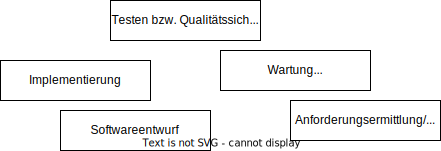
\includegraphics[scale=1.0]{Bilder/Kapitel-2/Abb-2-1.pdf}
    \caption{Kernprozesse des Softwareengineering}
    \label{fig:prozesse_softwareengineering}
\end{figure}

Die Einordnung von Prozessen und Teilprozessen in kausal-zeitliche Abfolgen ist Aufgabe von \textit{Vorgehensmodellen}. 
\marginline{von Prozessen\\zu Vorgehens\-modellen}
Im Rahmen des Softwareengineering beschreiben Vorgehensmodelle, \textbf{wie} der Entwicklungsvorgang von Softwareprodukten ablaufen soll. Je nach Zielrichtung des Vorgehensmodells werden dafür die einzelnen Prozesse und Teilprozesse des Softwareentwicklungsprozesses in bestimmter Reihenfolge und mit bestimmter Schwerpunktsetzung zusammengesetzt, wobei (Teil)Prozese auch wiederholt stattfinden können. Ergebnis ist die Definition eines idealtypisch ablaufenden Softwareentwicklungsprozesses. Für die Entwicklung eines \textbf{konkreten} Softwareprodukts müssen innerhalb des Rahmens des gewählten Vorgehensmodells dann die durchzuführenden konkreten Teilprozesse, Aktivitäten und Aufgaben für die Erstellung des Softwareprodukts bestimmt werden.

% 2.1
\clearpage
\section{Vorgehensmodelle – Ziele und Abgrenzungen}
\label{sec:Kap-2.1}

Die Wahl (und projektspezifische Anpassung) eines Vorgehensmodells gehört als Teil der Projektplanung zu den unterstützenden Prozessen des Softwareengineering und wird dementsprechend in vielen Softwareengineering-Lehrbüchern auch thematisiert. Gleichzeitig findet man Vorgehensmodelle auch in allgemeiner Literatur zum Thema Projektmanagement, da Vorgehensmodelle nicht auf IT-Projekte beschränkt sind.

Vorgehensmodelle stammen ursprünglich aus der Produktionstechnik. Sie unterteilen einen (Produktions)Prozess in logische Abschnitte und definieren zeitliche Abfolgen dieser Prozessabschnitte. Für jeden Prozessabschnitt werden Eintrittsvoraussetzungen, benötigte Ressourcen, durchzuführende Aktivitäten und zu produzierende Ergebnisse (Teilprodukte) festgelegt. Ziel ist es, den Erstellungsprozess eines Produkts so in planbare und kontrollierbare Einheiten zu unterteilen, dass die Erstellung des Produkts mit seinen vorgesehenen Funktionalitäten unter Einhaltung der veranschlagten Zeit- und Kostenbudgets mindestens unterstützt, im Idealfall sogar gesichert wird. Vorgehensmodelle sind in der Regel nicht auf ein einzelnes Produkt ausgerichtet, sondern beschreiben modellhaft abstrahierend und idealisiert Erstellungsprozesse für Kategorien von Produkten. So können (bewährte) Produktionsprozesse wiederholt und auch für andere Produkte übernommen werden.

\minisec{Vorgehensmodelle im Softwareengineering}

Einen idealen Softwareentwicklungsprozess, den man für jede beliebige Softwareentwicklung anwenden könnte, wird es nie geben. Die Menge der durchzuführenden Aufgaben für die Entwicklung eines Softwareprodukts, die Abhängigkeiten und die Reihenfolge dieser Aufgaben und damit auch die Abfolge der sie beinhaltenden (Teil)Prozesse ist spezifisch je nach Softwareentwicklungsprojekt. Vorgehensmodelle können Softwareentwicklungsprozesse jedoch ein Stück weit standardisieren. Sie sind Modelle für die Entwicklung von Softwareprodukten und werden in größerem Maße seit den 1980er Jahren eingesetzt. Sie geben einen (je nach Vorgehensmodell mehr oder weniger flexiblen) Rahmen für die auszuführenden Arbeitsschritte während eines Softwareentwicklungsprozesses vor. Ihr Einsatz soll insbesondere folgende Ziele erfüllen: 
\begin{itemize}
	\item die Komplexitätsreduktion des Softwareentwicklungsprozesses
	\item die Möglichkeit, Softwareprodukte in (großen) Teams zu erstellen
	\item die Sicherstellung von Prozess- und Produktqualität
	\item die strukturierte Steuerung und Kontrolle konkreter Softwareentwicklungsprozesse
	\item die Wiederholbarkeit von (bewährten) Methoden und Vorgehensweisen
	\item die Optimierung bestehender Prozesse bezüglich Zeit, Kosten und Qualität
\end{itemize}

Heute werden im Softwareengineering viele unterschiedliche Vorgehensmodelle eingesetzt. Sie unterscheiden sich unter anderem darin, wie detailliert sie die Abhängigkeiten und Abfolgen der einzelnen (Teil)Prozesse festlegen und in welchem Umfang sie durchzuführende Aufgaben vorgeben, und damit letztlich in der Frage, wie viel Raum sie der Individualität eines konkreten Softwareentwicklungsprozesses geben.

Manche Vorgehensmodelle legen den Fokus auf einzelne Softwareentwicklungsprojekte während andere aus einem höheren Blickwinkel die gesamte Softwareentwicklungsprojekt durchführende Organisation (Firma, Institution) betrachten. Einige Vorgehensmodelle lassen sich auch für beide Ebenen anwenden. In diesem Text betrachten wir nur auf Entwicklungsprojekte bezogene Vorgehensmodelle. Diese werden in der Literatur auch als \textit{Prozessmodelle} bezeichnet. In jüngerer Zeit begegnet einem zudem häufiger auch der Begriff des \textit{Entwicklungsmodells}. Im Englischen werden projektbezogene Vorgehensmodelle mit dem Begriff \textit{Software Life Cycle Model} bezeichnet, 
\marginline{Software-Lebenszyklus}
womit begrifflich der Gegenstandsbereich von Vorgehensmodellen, nämlich der Software-Lebenszyklus, deutlicher wird als in den deutschen Bezeichnungen. Unter einem Software-Lebenszyklus versteht man im engeren Sinne den Prozess von der Erhebung der Anforderungen an die zu erstellende Software bis zur Auslieferung des fertigen Softwareprodukts, im Englischen auch als Software Development Life Cycle (SDLC) bezeichnet. Das Wort Zyklus im Begriff trägt dabei der Tatsache Rechnung, dass auch ein fertiges Softwareprodukt überarbeitet werden und somit der Softwareentwicklungsprozess wieder von vorne beginnen kann. Erweiterte Definitionen ergänzen den SDLC um weitere Prozesse wie zum Beispiel Einsatz, Wartung, Weiterentwicklung und Ausmusterung eines Softwareprodukts, aber auch um Prozesse aus den Bereichen Konfiguration und langfristige Qualitätssicherung zum Software Product Life Cycle (SPLC).

Von Vorgehensmodellen zu unterscheiden sind \textit{Qualitätsmodelle} und \textit{Reifegrad-
	\linebreak %%% für Druck
	modelle}, was aufgrund mancher Überschneidung aber nicht immer konsequent möglich ist. Für Informationen zu einem bestimmten Vorgehensmodell lohnt es sich daher auch in Literaturkapiteln zu Qualitäts- und Reifegradmodellen nachzuschlagen, vielleicht hat die jeweilige Autorin/ der jeweilige Autor das entsprechende Vorgehensmodell dort verortet. Qualitätsmodelle 
\marginline{Qualitäts\-modelle}
bestimmen Qualitätsmerkmale und geben für diese Merkmale Qualitätskriterien und Maßsysteme vor, mit denen die Qualität von Softwareprodukten oder von Softwareentwicklungsprozessen bewertet werden kann. Viele Vorgehensmodelle beinhalten selber keine expliziten Vorgaben zu Qualitätssicherungsmaßnahmen. Konkrete Softwareentwicklungsprojekte, die nach solchen Vorgehensmodellen arbeiten, verwenden daher meist zusätzlich Qualitätsmodelle als Referenz für die Sicherstellung der Qualität ihrer Software oder ihres Entwicklungsprozesses.

Reifegradmodelle (engl. software process assessment model) 
\marginline{Reifegrad\-modelle}
bemessen die Fähigkeit einer Organisation (Softwareentwicklungs)Projekte durchzuführen. Sie tragen ihren Namen aufgrund der von ihnen definierten sogenannten Reifegradstufen, auf denen sich eine Organisation befinden kann. Der Reifegrad sagt aus, wie stark Softwareentwicklungsprozesse in der Organisation schon institutionalisiert sind. Dazu sind jeder Reifegradstufe eine Menge von Anforderungen zugeordnet, die eine Organisation erfüllen muss, um die entsprechende Reifegradstufe zu erreichen. Beispiele für Reifegradmodelle sind CMMI und SPICE\footnote{CMMI: Capability Maturity Model Integration; SPICE: Software Process Improvement and Capability Determination. Für eine Einführung in diese beiden Modelle siehe \cite[565-590]{bal08}. Zu Reifegradmodellen im Allgemeinen siehe \cite[Kap. 8]{swe14} und \cite{sha11}.}. Reifegradmodelle werden wir nicht behandeln.

\pagebreak %%% für Druck

Aufgrund der Unterschiedlichkeit 
\marginline{Vorgehens\-modelle legen strukturierte Verfahren fest} % dieser Absatz
der im Softwareengineering eingesetzten Vorgehensmodelle lässt sich nicht allgemeingültig aufzählen, welche Elemente Vorgehensmodelle genau enthalten und welche Vorgaben sie machen. Allen Vorgehensmodellen gemeinsam ist, dass sie strukturierte Verfahren für die Entwicklung von Softwareprodukten festlegen. So können Reihenfolgen von Prozessen vorgegeben, zu erstellende Artefakte des Entwicklungsprozesses festgelegt und Abfolgen durchzuführender Arbeitsschritte bestimmt werden. Je nach konkretem Vorgehensmodell kann es zusätzlich zum Beispiel Festlegungen zu benötigten Rollen und Kompetenzen, anzuwendenden Methoden oder einzusetzenden Entwicklungswerkzeugen geben. In anderen Vorgehensmodellen drückt sich strukturiertes Verfahren statt durch die Vorgabe von Prozessreihenfolgen dagegen eher durch die Vorgabe grundsätzlicherer Leitlinien und Prinzipien (\zb „den Auftraggeber institutionalisiert ins Projekt einbinden“, „nur lauffähigen Code einchecken“, „gemeinsames Code-Eigentum“) und fester Kommunikationsformate aus.

% 2.2
\clearpage
\section{Kategorien von Vorgehensmodellen}
\label{sec:Kap-2.2}

Konkrete Vorgehensmodelle unterscheiden sich mindestens darin, in welcher Granularität sie die durchzuführenden Tätigkeiten in einem Software\-entwicklungs\-projekt vorgeben. Doch deutlich stärkere Unterschiede zwischen Vorgehensmodellen finden sich, wenn diese unterschiedlichen \textit{Paradigmen} folgen.
\marginline{Paradigma}
Ein Paradigma ist eine grundsätzliche Denkweise/Lehrmeinung, man findet als Synonyme auch die Begriffe Weltanschauung oder Weltbild. Möglicherweise ist Ihnen der Begriff des Paradigmas in der Informatik aus dem Bereich der Programmierung bekannt. Programmier\-sprachen folgen einem Programmierparadigma -- wie zum Beispiel dem objekt-
\linebreak %%% für Druck
orientierten Paradigma --, wenn sie bestimmte im Paradigma festgelegte \mbox{Prinzipien} einhalten.

\begin{figure}[h!]
	\centering
	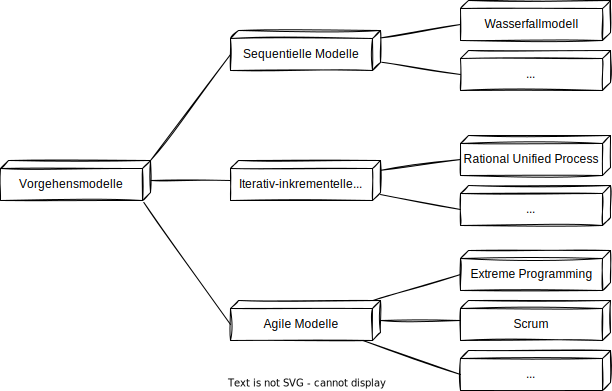
\includegraphics[scale=0.9]{Bilder/Kapitel-2/vorgehensmodelle.pdf}
	\caption{Kategorien von Vorgehensmodellen}
	\label{fig:vorgehensmodelle_komplett}
\end{figure}

Die ersten im Softwareengineering eingesetzten Vorgehensmodelle folgten einem Paradigma, das man als \textit{plangesteuert} bezeichnet. Diesem plangesteuerten Paradigma liegt die Einschätzung zugrunde, dass Softwareentwicklungsprojekte nur dann erfolgreich abgeschlossen werden können, wenn die durchzuführenden (Teil)Prozesse des Softwareengineering und ihr kausal-zeitlicher Ablauf im Vorfeld des Projekts systematisch geplant werden und spätere (Teil)Prozesse immer erst bei Vorliegen von vollständigen, qualitätsgesicherten und dokumentierten Ergebnissen vorhergehender Prozesse starten. Vorgehensmodelle, die dem plangesteuertem Paradigma folgen, gehören zur Kategorie der sogenannten \textit{sequentiellen Modelle} 
\marginline{sequentielle Modelle} 
oder Phasenmodelle. Der bekannteste Repräsentant sequentieller Modelle ist das Wasserfallmodell.

Im Unterschied zum plangesteuerten Paradigma wird im sogenannten agilen Paradigma, das seit Ende der 1990er Jahre verstärkt propagiert wird, die Einschätzung vertreten, dass ein Softwareentwicklungsprojekt nur dann erfolgreich abgeschlossen werden kann, wenn im Projektverlauf Änderungen zugelassen werden können, im Besonderen Änderungen der Anforderungen, und schon ab frühen Zeitpunkten im Projektverlauf lauffähiger (aber auch wieder änderbarer) Programmcode erzeugt wird. Vorgehensmodelle, die dem agilen Paradigma folgen, nennt man 
\marginline{agile Modelle} 
\textit{agile Modelle}. Bekannte Repräsentanten sind Extreme Programming und Scrum.

Sowohl sequentielle als auch agile Modelle werden heute im Softwareengineering eingesetzt. Konkrete Vorgehensmodelle – sowohl diejenigen, die wir in diesem Text vorstellen als auch die vielen anderen, die wir hier nicht thematisieren – passen in der Regel nicht hundertprozentig in genau eine Kategorie, da sie zusätzlich oft auch Kennzeichen anderer Kategorien aufweisen. In der Praxis gilt dies umso mehr, je stärker die Grundform eines Vorgehensmodell individuell an unternehmensspezifische Belange angepasst wird.

Wir werden in den folgenden Abschnitten sowohl allgemeiner die Kennzeichen sequentieller Modelle (Kap.~\ref{sec:Kap-2.2.1}) und agiler Modelle (Kap.~\ref{sec:Kap-2.2.3}) als auch konkrete Vorgehensmodelle als Repräsentanten dieser Kategorien von Vorgehensmodellen vorstellen. Abschnitt~\ref{sec:Kap-2.2.2} thematisiert zwischen der Vorstellung der sequentiellen und der Vorstellung der agilen Modelle eine dritte Kategorie von Vorgehensmodellen, die \textit{inkrementellen und iterativen Modelle}, 
\marginline{inkrementelle und iterative Modelle}
die in den späten 1980er und frühen 1990er Jahren erstmalig vorgestellt wurden und damit auch in ihrer Entstehungszeit zwischen den sequentiellen und den agilen Modellen liegen. Deren zugrundeliegendes Paradigma betont den Stellenwert der fachlichen Aspekte (Strukturen, Geschäftsprozesse etc.) des Einsatzgebiets des zu entwickelnden Softwareprodukts – und kritisiert damit auch die in der Regel sehr technisch orientierte Sichtweise von sequentiellen Vorgehensmodellen. Zum anderen beinhaltet es die Einschätzung, dass für erfolgreich durchzuführende Softwareentwicklungsprojekte lauffähiger Programmcode nicht erst am Ende des Projekts vorliegen darf – hier wurde die Basis für die Programmcode-Fokussierung der späteren agilen Modelle gelegt. 

\minisec{Unterscheidungsmerkmale zwischen Vorgehensmodellen}

Sequentielle, iterativ-inkrementelle (synonym: inkrementell-iterativ) und agile Vorgehensmodelle unterscheiden sich vor allem in folgenden Aspekten, die wir bei der Vorstellung der drei Kategorien in den folgenden Abschnitten jeweils im Detail betrachten werden:

\begin{enumerate}
	\item In welcher Weise werden die einzelnen (Teil)Prozesse zum Softwareentwicklungsprozess zusammengestellt?
	\item Wie wird mit neuen oder veränderten Anforderungen während der Entwicklung umgegangen?
	\item Inwieweit werden Auftraggeber und zukünftige Nutzer des zu erstellenden Softwareprodukts in die Entwicklung einbezogen?
	\item Zu welchen Zeitpunkten liegen auslieferungsfähige Produkte bzw. Teilprodukte vor?
	\item Welche Formen von Artefakten (\zb Programmcode, Dokumente, Modelle) entstehen im Laufe des Softwareentwicklungsprozesses?
\end{enumerate}

\subsection{Sequentielle Modelle}
\label{sec:Kap-2.2.1}

\vspace{\baselineskip} %%% für Druck

\sttpLeserfuehrung{Bilder/Kapitel-2/Leserfuehrung/vorgehensmodelle_sequentiell_illustration.pdf}{Bilder/Kapitel-2/Leserfuehrung/vorgehensmodelle_sequentiell.pdf}

\sttpHervorhebung{\textbf{Sequentielle Vorgehensmodelle}}
\marginline{Entwicklungs\-prozess}
\sttpHervorhebung{\textbf{unterteilen die Softwareentwicklung in aufeinanderfolgende zeitliche Abschnitte (Phasen)}}. 
Dafür werden zunächst die Tätigkeiten, die zur Entwicklung eines auslieferbaren Softwareprodukts notwendig sind, zu Prozessen zusammengefasst (\zb Prozess der Anforderungsanalyse, Prozess der Implementierung). Jedem Prozess entspricht dann eine Phase des sequen\-tiel\-len Vorgehensmodells. Es wird festgelegt, in welcher Reihenfolge die Phasen nacheinander durchlaufen werden. Zudem werden für jede Phase Start- und Endpunkt geplant, die zu erreichenden Ergebnisse definiert, die auszuführenden Tätigkeiten zur Erreichung dieser Ergebnisse spezifiziert, notwendige Input- und Output-Dokumente bestimmt sowie die durchzuführenden Qualitätssicherungs- und Controllingmaßnahmen festgelegt. 

Sequentielle Vorgehensmodelle sehen eine starke Aufgabenteilung vor. So sind einige Mitarbeiter für die Planung des Softwareentwicklungsprojekts, andere für die Implementierung und wieder andere für das Testen des fertigen Softwareprodukts zuständig. Die in einer Phase als Ergebnis produzierten Artefakte werden somit häufig von \textbf{anderen} Mitarbeitern in folgenden Phasen weiterverarbeitet. Sie müssen dementsprechend vollständig und verständlich sein. Eine Phase in einem sequen\-tiel\-len Vorgehensmodell kann erst beginnen, wenn die vorhergehende Phase komplett abgeschlossen wurde, was in der Regel durch das Erreichen von zuvor definierten Meilensteinen ausgedrückt wird. In einem ideal ablaufenden Projekt ist die Kontrolle des Projektfortschritts durch die im Vorfeld terminierten Meilensteine sehr einfach. 

\vspace{\baselineskip} %%% für Druck

\sttpDefinitionskasten{\sttpDefinitionskastenSkalierungsfaktor}{Meilenstein}{Ein überprüfbares Zwischenziel innerhalb eines Projekts.}{Meilensteine werden zu Beginn eines Projekts definiert und zeitlich festgelegt. Im Laufe des Projekts kann anhand der erreichten und noch nicht erreichten Meilensteine der Projektfortschritt und der ggf. bestehende Zeitverzug im Projekt bestimmt werden. Der Begriff Meilenstein stammt aus dem klassischen Projektmanagement.}

\vspace{\baselineskip} %%% für Druck

Die strenge Form des sequentiellen Vorgehensmodells sieht vor, dass jede Phase nur genau einmal durchlaufen wird, die Phasen überschneidungsfrei sind und dementsprechend auch niemals in eine bereits abgeschlossene Phase zurückgekehrt werden kann. Dem liegt die idealisierte Vorstellung zugrunde, dass jede Phase fehlerfrei abgearbeitet werden kann und auf dieser optimalen Basis dann die folgende Phase beginnen kann. In der Praxis trifft das selten zu. Die Vorgabe, jede Phase nur einmal zu durchlaufen, würde zum Beispiel bedeuten, auch dann nicht in eine Entwurfs\-phase zurückkehren zu können, wenn Fehler oder Unvollständigkeiten des Entwurfs erst während der Implementierung auffallen. Man müsste auf Grundlage des fehlerhaften oder unvollständigen Entwurfs weiterarbeiten – wodurch das entstehende Softwareprodukt nicht (alles) das tut, was es tun soll –, oder bei der Implementierung ganz bewusst vom vorliegenden Entwurf abweichen. Letzteres würde implizit Entwurfsaktivitäten in die Phase der Implementierung verlagern, was dem Charakter eines sequentiellen Vorgehensmodells widerspricht, weil es das Konzept der inhaltlich abgegrenzten Phasen unterläuft. Die in der Praxis eingesetzten sequen\-tiel\-len Vorgehensmodelle sehen fast immer iterative Elemente vor. So kann zumindest in die zuvor abgeschlossene Phase zurückgekehrt werden, sofern Fehler, Unvollständigkeiten oder Unklarheiten bestehen. Die entsprechende Phase wird somit erneut durchlaufen und die Ergebnisse der Phase werden entsprechend angepasst. Abbildung~\ref{fig:prozesse_softwareengineering_sequentiell} zeigt Prozesse des Softwareengineering in einer sequentiellen Abfolge.

\begin{figure}[h!]
    \centering
		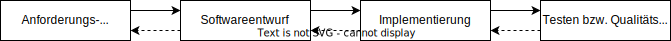
\includegraphics[width=1.0\textwidth]{Bilder/Kapitel-2/Abb-2-3.pdf}
    \caption[Prozesse des Softwareengineering in sequentieller Abfolge]{Prozesse des Softwareengineering in der sequentiellen Abfolge Anforderungsermittlung-Entwurf-Implementierung-Testen. Die gestrichelten Pfeile stellen die Rückkehrmöglichkeiten in die jeweils vorhergehende Phase dar.}
    \label{fig:prozesse_softwareengineering_sequentiell}
\end{figure}

\sttpHervorhebung{\textbf{Sequentielle Vorgehensmodelle}} 
\marginline{Umgang mit Anforderungen} 
\sttpHervorhebung{\textbf{definieren sämtliche Anforderungen zu Projektbeginn.}}
Dieser Katalog an Anforderungen bildet bei Auftragsarbeiten in der Regel auch die inhaltliche Grundlage für den Vertragsabschluss zwischen dem Auftraggeber und der Firma oder Institution, die die Softwareentwicklung übernimmt. Änderungen und Ergänzungen in Bezug auf die Anforderungen sind überhaupt nur dann möglich, wenn im Vorfeld zwischen Auftraggeber und Auftragnehmer (rechtlich) eindeutige Änderungsprozesse – vor allem in Bezug auf die Kostenübernahme – definiert wurden. Die sequentiellen Modelle eignen sich daher am besten für Projekte, deren Anforderungen von Anfang an vollständig und präzise definiert sind und in denen die Anforderungen auch über die Projektlaufzeit stabil bleiben. Implizit setzen sequentielle Vorgehensmodelle zudem voraus, dass das Softwareentwicklungsteam über einen erfahrenen Projektleiter verfügt, der anhand der Anforderungen eine realistische Abschätzung bezüglich Zeitaufwand und Kosten der Entwicklung vornehmen kann.

\sttpDefinitionskasten{\sttpDefinitionskastenSkalierungsfaktor}{Projektleiter}{Diejenige Rolle, die für ein konkretes Softwareentwicklungsprojekt organisatorische und koordinierende Aufgaben übernimmt.}{Wir verwenden den Begriff in einem sehr weiten Sinne. Die Person, die die Rolle Projektleiter übernimmt, kann gleichzeitig Personalführungsverantwortlichkeiten besitzen oder selber auch Entwicklungstätigkeiten ausführen oder mehrere Projekte leiten etc. Je nach Unternehmen bzw. Vorgehensmodell kann diese Rolle auch die Bezeichnung Projektmanager, Entwicklungsleiter, Scrum Master etc. tragen.}

\sttpHervorhebung{\textbf{Sequentielle Vorgehensmodelle}} 
\marginline{Einbezug Kunde}
\sttpHervorhebung{\textbf{binden Auftraggeber oder zukünftige Nutzer eher weniger ein.}} 
Auftraggeber und zukünftige Nutzer des Softwareprodukts werden nur zu Beginn des Projekts in den Prozess der Anforderungsermittlung einbezogen. Alle späteren Entwurfs- und Implementierungstätigkeiten sowie auch ein großer Teil der Test\-akti\-vitäten finden nur innerhalb des Entwicklungsteams statt. Dem Auftraggeber wird das Produkt erst am Ende des Projekts zur sogenannten Abnahme – Prüfung, ob das Produkt die vertraglich vereinbarte Leistung erbringt – wieder vorgelegt.

\sttpHervorhebung{\textbf{Sequentielle Vorgehensmodelle}}
\marginline{Artefakte}
\sttpHervorhebung{\textbf{sind dokumentenorientiert.}}
Als Ergebnis einer Phase entstehen ein oder mehrere Dokumente (\zb Pflichtenheft, Entwurfs\-spezifikation, Diagramm der Systemmodule), die Grundlage der nächsten Phase sind und dort weiter verfeinert, ergänzt oder angepasst werden. Eine große Heraus\-forderung besteht darin, diese Dokumente untereinander, aber auch in Bezug auf den endgültigen Programmcode des Softwareprodukts, während des gesamten Entwicklungsprozesses konsistent zu halten.
%\sttpgls{Konsistenz}

\sttpHervorhebung{\textbf{Sequentielle Vorgehensmodelle}} 
\marginline{Auslieferung}
\sttpHervorhebung{\textbf{liefern das Produkt erst mit Ende des Softwareentwicklungsprojekts aus.}} 
Zwar können auch während des Entwicklungsprozesses bereits lauffähige Versionen mit Teilfunktionalität existieren, doch werden diese nicht für den produktiven Einsatz herausgegeben.

Ein bekannter Vertreter sequentieller Vorgehensmodelle ist das Wasserfallmodell. Es ist das erste Vorgehensmodell, das in großem Maße im Softwareengineering eingesetzt wurde.

\clearpage %%% für Druck

\subsubsection{Wasserfallmodell(e)}
\label{sec:Kap-2.2.1.1}

\vspace{\baselineskip} %%% für Druck

\sttpLeserfuehrung{Bilder/Kapitel-2/Leserfuehrung/vorgehensmodelle_sequentiell_illustration.pdf}{Bilder/Kapitel-2/Leserfuehrung/vorgehensmodelle_wasserfall.pdf}

Die Überschrift deutet es schon an: Eigentlich ist es falsch von \textbf{dem} Wasserfallmodell zu sprechen, da es Wasserfallmodelle heute in vielen Varianten gibt. Dementsprechend unterschiedliche Abbildungen findet man in der Literatur.

\minisec{Historische Wasserfallmodelle} 

Das ursprüngliche Wasserfallmodell stellte Winston W. Royce 1970 vor \cite{roy70}. \mbox{Royce} orientierte sich für sein Modell an der Darstellung eines sequentiellen Prozessmodells aus den 1950er Jahren\footnote{Das sogenannte \textit{stagewise model}, ein Prozessmodell für die Systementwicklung des Semi-Automatic Ground Environment Systems (SAGE), das erste computergestützte Luftverteidigungssystem Nordamerikas (USA, Kanada). 1956 von Herbert D. Benington beschrieben \cite{ben56}, zusammenfassend zum Modell \cite[43\psq]{kne17}.}, verdichtete dessen ursprünglich neun Phasen zu sieben, ergänzte sogenannte Rückkopplungsmöglichkeiten (Rückkehr von einer Phase in die vorhergehende Phase) und führte die an einen Wasserfall erinnernde Darstellung ein. Abbildung~\ref{fig:wasserfallmodel_nach_royce} zeigt das Wasserfallmodell von Royce.  

\begin{figure}[h!]
    \centering
    \includegraphics[width=1.0\textwidth]{Bilder/Kapitel-2/WasserfallmodellRoyce.pdf}
    \caption[Wasserfallmodell von Royce]{Wasserfallmodell von Royce, nach \cite[330]{roy70}}
    \label{fig:wasserfallmodel_nach_royce}
\end{figure}

\pagebreak %%% für Druck

In mancher Literatur findet sich die Unterscheidung zwischen einem Wasserfall\-modell \textbf{ohne} und einem Wasserfallmodell \textbf{mit} Rückkehrmöglichkeit in die vorhergehende Phase. Dies ist allerdings ein Irrtum, der darauf zurückzuführen ist, dass der Artikel von Royce zur Hinführung auf sein Modell auch wasserfallartige Abbildungen ohne Rückkehrmöglichkeiten enthält. Das von ihm vorgeschlagene Modell sieht die Rückkopplung zur jeweils vorhergehenden Phase aber explizit vor. Kaum in Erinnerung geblieben ist zudem, dass Royce eng verknüpft mit seinem Modell Maßnahmen zur Reduzierung von Entwicklungsrisiken vorschlägt, die man heute erst später entstandenen Vorgehensmodellen zuordnet. Dazu gehören eine kontinuier\-liche Einbeziehung der zukünftigen Nutzer (in Royce' Modell noch an festen Punkten im Projektablauf) und das Arbeiten mit Prototypen 
%\sttpgls{Prototyp}
(er verwendet den Begriff pilot model).

Vermehrt eingesetzt für die Softwareentwicklung werden Wasserfallmodelle seit den Veröffentlichungen von Barry W. Boehm  in den 1980er Jahren. Abbildung~\ref{fig:wasserfallmodel_nach_boehm} zeigt das Wasserfallmodell von Boehm.  

\begin{figure}[h!]
    \centering
    \includegraphics[scale=0.75]{Bilder/Kapitel-2/WasserfallmodellBoehm.pdf}
    \vspace{\baselineskip} %%% für Druck
    \caption[Wasserfallmodell von Boehm]{Wasserfallmodell von Boehm, nach \cite[36]{boe81}}
    \label{fig:wasserfallmodel_nach_boehm}
\end{figure}

\pagebreak %%% für Druck

Boehm erweiterte Anfang der 1980er Jahre das Modell von Royce, indem er den Zuschnitt der einzelnen Phasen veränderte, den Punkt der Softwarewartung (engl. maintenance) ergänzte und Qualitätssicherungsaspekte explizit ins Modell aufnahm. Boehm war zudem derjenige, der den Namen Wasserfallmodel populär machte.

\minisec{Heutige Wasserfallmodelle}

Heute findet man überwiegend fünf- und sechsphasige Wasserfallmodelle. Abbildung~\ref{fig:wasserfallmodel_fuenf_phasen} zeigt links ein beispielhaftes fünfphasiges Wasserfallmodell und rechts ein sechsphasiges. 

\begin{figure}[h!]
    \centering
		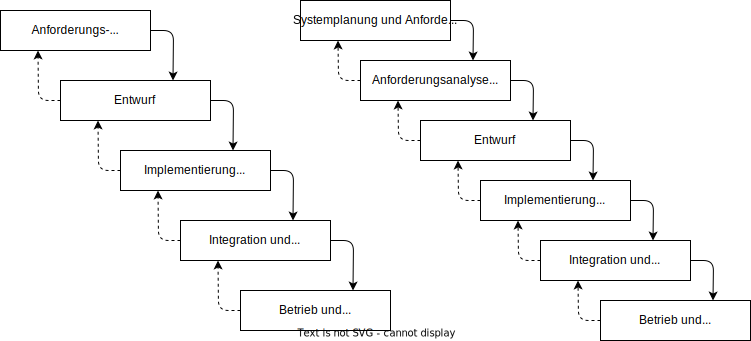
\includegraphics[width=1.0\textwidth]{Bilder/Kapitel-2/Abb-2-6.pdf}%
    \caption{Beispielhaftes fünf- bzw. sechsphasiges Wasserfallmodel}
    \label{fig:wasserfallmodel_fuenf_phasen}
\end{figure}

Im Vergleich zu fünfphasigen werden bei sechsphasigen Wasserfallmodellen meistens explizit Tätigkeiten der Planung des Softwareentwicklungsprojekts (\zb Kalkulation, Projektplan) integriert und der Prozess rund um die Spezifizierung von Anforderungen auf zwei Phasen aufgeteilt. Zum Beispiel sind die Erstellung von Lastenheft 
%\sttpkapitelverweis{Lastenheft und Pflichtenheft}{Kap.~\ref{sec:Kap-6.2.5}}
und Pflichtenheft bei fünfphasigen Modellen üblicherweise beide Teil der ersten Phase, während bei sechsphasigen Modellen die Erstellung des Pflichtenhefts erst zur zweiten Phase gehört. 

Die Wasserfallmodelle in Abbildung~\ref{fig:wasserfallmodel_fuenf_phasen} sind nur beispielhafte Ausprägungen fünf- und sechsphasiger Wasserfallmodelle. Die in konkreten Softwareentwicklungsprojekten eingesetzten Wasserfallmodelle unterscheiden sich von diesen Abbildungen, aber auch untereinander, oftmals im konkreten Zuschnitt und damit auch in der Benennung der einzelnen Phasen. Dies betrifft insbesondere den Bereich des Testens, bezogen auf die Abbildungen damit die Trennung zwischen der Phase Implementierung und Modultests %\sttpgls{Softwaretests} 
und der folgenden Phase Integration und Systemtest. Hier reicht das Spektrum von der kompletten Auslagerung des Testens in die spätere Phase – womit in der Implementierungsphase nur reine „Debugging-Tests“ stattfinden – bis zur Durchführung kompletter Integrationstests in der früheren Phase – womit in der späteren Phase nur noch der Systemtest verbleibt. 

\minisec{Struktur des Softwareentwicklungsprozesses}

\vspace{1.5mm} %%% für Druck

Das Wasserfallmodell ist ein sehr starres sequentielles Vorgehensmodell. Es sieht vor, dass mit einer Phase erst dann begonnen wird, wenn sämtliche Aktivitäten der vorherigen Phase abgeschlossen wurden und die entstandenen Ergebnisse qualitätsgesichert sind – dementsprechend alle Meilensteine erreicht sind. Der zu Beginn des Softwareentwicklungsprozesses einmal festgelegte Ablauf der abzuarbeitenden Aktivitäten wird nach Möglichkeit eingehalten.

\vspace{0.6mm} %%% für Druck

Aus Managementsicht besticht das Wasserfallmodell damit vordergründig durch seine Einfachheit. Anhand von Meilensteinen ist der Projektfortschritt jederzeit kontrollierbar. Zu Beginn eines Projekts kann eine systematische Planung der benötigten Personalressourcen erfolgen. Aufgrund des unterschiedlichen inhaltlichen Zuschnitts der einzelnen Phasen und der umfangreichen Dokumentation der Ergebnisse einer Phase ist es dabei möglich, für verschiedene Phasen unterschiedliche (auch örtlich unverbundene) Teams einzusetzen. Schon zu Beginn des Projekts kann zum Beispiel kalkuliert werden, wann ein erfahrener Softwarearchitekt und wann das Team der Softwaretester benötigt wird. Die abgegrenzten Zuschnitte der Phasen und die Ausrichtung auf zu erreichende Meilensteine führen zudem in der Regel dazu, dass in einem Projekt auch die einzelnen Arbeitsaufgaben innerhalb einer Phase stark vorgegeben sind. Gerade für Softwareentwickler mit wenig Erfahrung kann das Orientieren an festen Vorgaben und das Abarbeiten begrenzter Aufgaben hilfreich sein.

\vspace{0.6mm} %%% für Druck

Auch wenn das Wasserfallmodell die Rückkehr in schon abgeschlossene Phasen vorsieht, hängen Umfang und Anzahl der möglichen Überarbeitungen in der Praxis davon ab, wieviel zeitlicher Puffer für das Projekt eingeplant wurde. Der Einsatz eines Wasserfallmodells erfordert daher einen erfahrenen Projektleiter, der den Projektplan und die einzelnen Arbeitsschritte zielführend und realistisch durchführbar festlegt und dabei im Projektplan auch ausreichende Zyklen (Rückkehr in bereits abgeschlossene Phasen) für eventuell notwendige Überarbeitungen von Ergebnissen vorsieht. 

\vspace{0.6mm} %%% für Druck

In der Praxis ist die vorgesehene Abgeschlossenheit der Phasen zudem nicht immer notwendig, zum Beispiel weil Komponenten des zu entwickelnden Softwareprodukts so unabhängig voneinander sind, dass mit der Implementierung einer Komponente (\zb Benutzerverwaltung) begonnen werden könnte, bevor der Entwurf für eine andere Komponente (\zb Seminarverwaltung) komplett erstellt ist. Außerdem  treten in den meisten Projekten Verzögerungen im Projektablauf ein, sei es weil Mitarbeiter ausfallen, Aufwände für Tätigkeiten falsch eingeschätzt wurden oder Fehler bemerkt werden, die zeitaufwändig korrigiert werden müssen. Die geringe Flexibilität des Wasserfallmodells macht es schwierig auf solche Risikofaktoren zu reagieren. Sofern der Auslieferungstermin der Software nicht verschoben werden kann, führen Verzögerungen im Projektablauf oft zur Verkürzung der späteren Phasen des Projekts. Da im Wasserfallmodell der Bereich des Testens die letzte Phase vor der Auslieferung der Software bildet, gehen solche Verzögerungen in der Regel zu Lasten der Testaktivitäten.

\vspace{0.6mm} %%% für Druck

Hinzu kommt, dass durch die späte Testphase 
\marginline{späte Testphase}
Fehler sowie unvollständige oder unklare Spezifikationen erst spät im Projektverlauf offensichtlich werden. Spät erkannte Fehler sind oft teurer als frühzeitig erkannte Fehler, da größere Personalressourcen für Arbeiten auf fehlerhafter Grundlage investiert wurden. Sollten beim Testen oder auch erst im Betrieb noch größere Fehler in der Software entdeckt werden, ist es zudem zu spät Grundlegendes zu ändern. Es bleiben dann nur noch provisorische Behelfslösungen (engl. Workarounds), die die Symptome des fehlerhaften Verhaltens der Software behandeln, aber nicht die grundlegenden Probleme lösen. Um solche Situationen zu vermeiden, sehen viele heutige Wasserfallmodelle schon parallel zur Implementierung Testaktivitäten vor (\zb Tests einzelner Komponenten). Der abschließende sogenannte Systemtest, bei dem die Software gegen alle spezifizierten Anforderungen getestet wird, findet in Wasserfallmodellen in der Regel aber weiterhin erst in der letzten Phase vor der Auslieferung statt. Sollte dabei das Fehlen von Funktionalitäten bemerkt werden, ist es in den meisten Fällen zu spät, daran etwas zu ändern.

\minisec{Umgang mit Anforderungen}

Die Anforderungen an das zu erstellende Softwareprodukt werden im Wasserfall\-modell ganz zu Beginn des Softwareentwicklungsprojekts ermittelt. Sobald die Anforderungsspezifikation 
%\sttpkapitelverweis{Anforderungsspezifikation}{Kap.~\ref{sec:Kap-6.1.x}} 
erstellt und (vom Auftraggeber) geprüft wurde, können in der Regel keine neuen oder veränderten Anforderungen berücksichtigt werden. Das ist ein Problem: Zwischen der Planung eines Softwareentwicklungsprojekts und der Auslieferung des fertigen Produkts können durchaus mehrere Jahre liegen. In dieser Zeit können sich Arbeitsprozesse sowie Erfahrungen und Erwartungen von Nutzern schon derart verändert haben, dass das entwickelte Produkt die Bedürfnisse seiner Nutzer schon zum Zeitpunkt seines Ersteinsatzes nicht mehr erfüllt. Hinzu kommt, dass es nur selten wirklich möglich ist die Anforderungen zu Projektbeginn hundertprozentig vollständig und unmissverständlich zu erfassen.

\vspace{2mm}

\sttpDefinitionskasten{\sttpDefinitionskastenSkalierungsfaktor}{Kunde}{Auftraggeber oder Nutzer des Softwareprodukts.}{Wir verwenden den Begriff Kunde als Verallgemeinerung in Kontexten, in denen eine Unterscheidung zwischen Auftrag\-geber auf der einen Seite und Nutzer auf der anderen Seite nicht sinnvoll bzw. möglich ist.}

\minisec{Einbezug des Kunden}

Die Einbindung des Auftraggebers oder zukünftiger Nutzer des Softwareprodukts in den Prozess der Softwareentwicklung ist nur in der Zeit der Anforderungsermittlung/
\linebreak %%% für Druck
-analyse vorgesehen. In der Praxis kommt es natürlich trotzdem vor, dass auch in späteren Phasen bei Unklarheiten mit dem Auftraggeber Rücksprache gehalten wird, eine systematische Rücksprache in der Entwurfsphase (oder sogar in der Implementierungsphase) sieht das Wasserfallmodell aber nicht vor. Das kann auch bei im Projektverlauf stabilen Anforderungen leicht dazu führen, dass die wirklichen Vorstellungen der Kunden im fertigen Produkt unzureichend umgesetzt sind.

Wichtig für die erfolgreiche Softwareentwicklung mit einem Wasserfallmodell ist, dass im Softwareentwicklungsteam eine sehr genaue Kenntnis des fachlichen Problembereichs vorliegt, um die fehlende Einbindung und das somit nicht vorhandene Feedback des Kunden kompensieren zu können.

\vspace{2mm} %%% für Druck

\minisec{Artefakte des Entwicklungsprozesses}

Als sequentielles Vorgehensmodell ist das Wasserfallmodell dokumentenorientiert. Ein Großteil der Tätigkeiten während des Softwareentwicklungsprozesses ist darauf ausgerichtet, verschiedene Dokumente
\marginline{Dokumente}
zu erstellen (\zb Anforderungsspezifikation, Architekturspezifikation, Komponentenmodell, Testplan). Die Meilensteine am Ende der Phasen beziehen sich dementsprechend auch meistens auf das Vorliegen bestimmter Dokumente, welche dann in der Regel die Basis für die Aktivitäten der folgenden Phase bilden. Aufgrund dieser dokumentenorientierten Ausrichtung entsteht während der Entwicklung des Softwareprodukts eine umfangreiche technische Dokumentation des Systems. Dies erleichtert die Einarbeitung neuer Mitarbeiter während des Projekts, aber auch die Einarbeitung derjenigen Mitarbeiter, die das erstellte Softwaresystem später betreiben sollen.

\vspace{2mm} %%% für Druck

\minisec{Einsatz von Wasserfallmodellen}

Trotz aller Kritikpunkte am Wasserfallmodell sollte man seine Bedeutung nicht geringschätzen. Zum einen hat das Wasserfallmodell viel dazu beigetragen, unter Softwareentwicklern ein Verständnis für die notwendige Trennung zwischen den fachlichen Anforderungen auf der einen Seite und ihrer technischen Umsetzung auf der anderen Seite zu etablieren. Zum anderen haben sich auf Basis des Wasserfallmodells und insbesondere auch anhand seiner Probleme andere Arten von Vorgehensmodellen herausgebildet, die es ohne die – schon in den 1980er Jahren geführte – intensive Diskussion über die Vor- und Nachteile des Wasserfallmodells vielleicht nicht geben würde.

In  der Literatur finden sich unterschiedliche Ansichten darüber, in welchen Situationen und für welche Institutionen und Projekte es auch heute noch sinnvoll ist, ein Wasserfallmodell als Vorgehensmodell zu verwenden. Als typische
\marginline{Anwendungs\-bereiche}
Anwendungs\-bereiche werden oft eingebettete Systeme (engl. embedded systems) und sicherheitskritische Systeme genannt. Bei eingebetteten Systemen übernimmt die Software die Steuerung der Hardware sowie die Interaktion mit der Außenwelt. Da sich die Hardware nicht verändern lässt, sobald sie produziert wurde, müssen die Aufgaben\-teilung zwischen Hardware und Software und damit die genauen Anforderungen an die Software zu Beginn der Entwicklung festgelegt werden. Genauso orientiert sich der Entwurf der Software an den Gegebenheiten der Hardware. Da ein eingebettetes System aufgrund der Inflexibilität der Hardware damit in der Regel sowieso schwer auf veränderte Anforderungen reagieren kann, steht dieser Aspekt auch für die entsprechende Softwareentwicklung nicht so sehr im Vordergrund. Für die Entwicklung sicherheitskritischer Systeme gilt eine Reihe von Vorschriften, die bei der Softwareentwicklung eingehalten werden müssen. Dazu gehören oft auch formale Analysen von Spezifikations- und Entwurfsdokumenten, die nachweisen sollen, dass die notwendigen sicherheitskritischen Anforderungen berücksichtigt sind. Da es sich dabei um einen aufwändigen und teuren Prozess handelt, der idealerweise nur einmalig im Laufe der Entwicklung des Softwareprodukts stattfindet, sollten die Entwurfs\-tätig\-keiten vollständig abgeschlossen sein, bevor die formalen Analysen durchgeführt werden. Aber auch wenn in Projekten für eingebettete oder sicherheitskritische Systeme vielleicht häufiger Wasserfallmodelle zu finden sind, bedeutet das nicht, dass dort andere Vorgehensmodelle gar nicht eingesetzt würden. Auf der anderen Seite kann man auch in anderen Anwendungsgebieten auf wasserfallartige Vorgehensmodelle treffen.

In der Praxis wird die Entscheidung für ein Vorgehensmodell 
\marginline{Entscheidung für ein Vorgehens\-modell}
häufig nicht aufgrund der expliziten Abwägung seiner Vor- und Nachteile gegenüber den Vor- und Nachteilen anderer Vorgehensmodelle getroffen werden, sondern aufgrund weicherer Faktoren: Ein Unternehmen, das mit einem Wasserfallmodell erfolgreich ein Produkt für einen Kunden entwickelt hat, wird bei einem ähnlichen Produkt für einen anderen Kunden vermutlich wieder ein Wasserfallmodell wählen. Ein Projektleiter, der bei seinem letzten Projekt die Einbindung des Kunden schmerzlich vermisst hat, wird versuchen diesen Aspekt im neuen Projekt zu verbessern und damit evtl. auch zu einem anderen Vorgehensmodell wechseln. Wasserfallmodelle (oder andere Arten von sequentiellen Modellen) werden seit über vierzig Jahren in Soft\-ware\-entwick\-lungs\-projekten eingesetzt. Viele Unternehmen, die Software für interne oder externe Zwecke entwickeln, haben daher Arbeitsprozesse in anderen Abteilungen als der Softwareentwicklungsabteilung auf solche Vorgehensmodelle ausgerichtet (\zb die Bereiche Auftragsaquise, Vertragswesen, Personalplanung, Controlling). Gerade der Umstieg von einem sequentiellen Wasserfallmodell auf agile Vorgehensmodelle erfordert oft auch Veränderungen der Arbeitsprozesse des Unternehmens, die teuer und aufwändig sind und daher vielleicht nur zögerlich vorgenommen werden. Viele Softwarehersteller haben zudem im Laufe der Jahre wasserfallartige Modelle so an ihre Bedürfnisse angepasst, dass in ihren unternehmensspezifischen Modellen nicht mehr alle Nachteile des ursprünglichen Wasserfallmodells zum Tragen kommen.

Abgesehen von institutionellen oder anderen Zwängen lässt sich festhalten: Wenn mit einer etablierten Technologie für ein Umfeld mit stabilen Anforderungen entwickelt wird, diese Anforderungen zu Beginn des Projekts definiert werden können und ein erfahrener Projektleiter zur Verfügung steht, dann kann man über den Einsatz eines Was\-ser\-fall\-modells nachdenken. In allen anderen Fällen sollten flexiblere Vorgehensmodelle gewählt werden.

\subsection{Inkrementelle und iterative Modelle}
\label{sec:Kap-2.2.2}

\sttpLeserfuehrung{Bilder/Kapitel-2/Leserfuehrung/vorgehensmodelle_iterativ_inkrementell_illustration.pdf}{Bilder/Kapitel-2/Leserfuehrung/vorgehensmodelle_iterativ_inkrementell.pdf}

Die  Spannweite an Modellen, die als inkrementelle Modelle bezeichnet werden können, ist groß. Sie reicht von Modellen, die stark sequentiellen Modellen ähneln bis zu solchen, die auch iterative oder agile Methoden einsetzen. Charakteristisch für inkrementelle Modelle sind zwei Aspekte: Das zukünftige Gesamtprodukt wird erstens in produktiv einsetzbaren, mit eigener Funktionalität ausgestatteten Teil\-produkten (sogenannten Inkrementen) entwickelt und ausgeliefert, und ausgelieferte Teil\-produkte werden zweitens (möglichst) nicht überarbeitet. 

\sttpDefinitionskasten{\sttpDefinitionskastenSkalierungsfaktor}{Inkrement}{Betrag, um den eine Größe zunimmt.}{In unserem Fall ist die Größe die Produktfunktionalität.}

Im Zusammenhang mit dem Aufkommen agiler Vorgehensmodelle Anfang der 2000er Jahre erfuhr diese „klassische“ Charakterisierung von inkrementellen Modellen eine leichte Begriffsaufweichung. Der Begriff Inkrement bezeichnet heute häufig das ausgelieferte Teilprodukt an sich, \textbf{unabhängig davon}, ob dieses in späteren Produktversionen noch überarbeitet werden kann oder nicht und (allerdings seltener) auch unabhängig davon, ob ein Inkrement neue eigene Funktionalität anbietet oder eine interne Überarbeitung (\zb Wechsel der Datenstruktur) eines vorherigen Inkrements darstellt. In der Literatur finden sich unter der Überschrift „inkrementelle Vorgehensmodelle“ dementsprechend unterschiedliche Darstellungen, abhängig davon, welche Vorstellung von Inkrement eine Autorin/ein Autor zugrunde gelegt hat. Wir verwenden in diesem Text die klassische Charakterisierung von inkrementell. Und auch wenn konkrete Vorgehensmodelle in der Regel nie rein inkrementell oder rein iterativ sind, sondern Kennzeichen beider Kategorien aufweisen und somit iterativ-inkrementelle Modelle sind, werden inkrementelle Modelle und iterative Modelle in diesem Abschnitt getrennt voneinander behandelt, um die Unterschiede deutlicher zu machen.

\sttpHervorhebung{\textbf{Inkrementelle Modelle}}
\marginline{Auslieferung}
\sttpHervorhebung{\textbf{liefern Teilprodukte aus.}}
Im  Unterschied zu sequen\-tiel\-len Vorgehensmodellen wird bei inkrementellen Modellen die zu erstellende Software nicht als ein komplettes Produkt am Ende des Entwicklungsprojekts ausgeliefert. Stattdessen werden mehrere Teilprodukte schrittweise entwickelt, ausgeliefert und eingesetzt, aus deren Kombination sich am Ende das Gesamtprodukt ergibt. Jedes neue Inkrement bringt dabei eigene Funktionalitäten mit und erweitert so die Gesamtfunktionalität der aktuell eingesetzten Produktversion.

Für die Aufteilung eines zu erstellenden Softwareprodukts in Teilprodukte gibt es nach Balzert \cite[526 \psq]{bal08} zwei grundsätzliche Vorgehensweisen: das puzzle\-artige Zusammensetzen von Teilprodukten zum Gesamtprodukt und das ausgehend von einem ersten Teilprodukt zwiebelschalenförmige schrittweise Ergänzen weiterer Teilprodukte. Abbildung~\ref{fig:inkrementelle_entwicklung} illustriert diese beiden Varianten. 

\begin{figure}[h!]
	\vspace{\baselineskip} %%% für Druck
	\begin{addmargin*}[0cm]{-\marginparwidth}
	\begin{addmargin*}[0cm]{-\marginparsep}
		\centering
		\includegraphics[width=1.2\textwidth]{Bilder/Kapitel-2/PuzzleZwiebel.pdf}
		\caption[Puzzleförmige und zwiebelschalenförmige inkrementelle Entwicklung]{Puzzleförmige (links) und zwiebelschalenförmige (rechts) inkrementelle Entwicklung, nach \cite[527]{bal08}}
		\label{fig:inkrementelle_entwicklung}
	\end{addmargin*}
	\end{addmargin*}
\end{figure}

Welche der beiden Arten 
\marginline{Entwicklungs\-prozess}
für ein konkretes Softwareentwicklungsprojekt eingesetzt werden sollte, hängt in erster Linie davon ab, in welcher Weise sich die Anforderungen an das Gesamtprodukt auf die geplanten Teilprodukte aufteilen lassen. Wenn sich die gewünschten Funktionalitäten annähernd eindeutig bestimmten Teilprodukten (\zb eine Passagierverwaltung und eine Flugzeugverwaltung für ein Flugreservierungssystem) zuordnen lassen, wird eher die puzzleartige Variante der inkrementellen Auslieferung zum Einsatz kommen. Bei der Planung der Inkremente müssen die zukünftigen Schnittstellen zwischen den Teilprodukten (in der Abbildung die Aus- und Einbuchtungen der Puzzleteile) dann so definiert werden, dass es im Ideal\-fall nicht nötig ist ein bestehendes Inkrement zu verändern, sobald ein weiteres Inkrement ergänzt wird.  Wenn dagegen geforderte Funktionalitäten unterschiedlicher Teilprodukte dieselbe Basis benötigen, ist es sinnvoll oder sogar zwingend notwendig, zunächst ein erstes Teilprodukt als Kern des Gesamtsystems zu entwickeln. Jedes weitere Inkrement baut dann so auf der vorherigen Pro\-dukt\-ver\-sion auf, dass es auf Basis der vorherigen Inkremente die Funktionalitäten des Produkts erweitert. Kombinationen beider Varianten der inkrementellen Auslieferung sind auch möglich, zum Beispiel falls alle Teilprodukte nur einen gemeinsamen Kern benötigen, ansonsten aber nicht aufeinander aufbauen müssen.

Die Entwicklung der Teilprodukte – auch bei puzzleförmiger Aufteilung – findet in der Regel nicht parallel, sondern zumindest versetzt statt (\zb Teilprodukt 1 schon im Einsatz, Teilprodukt 2 in der Entwicklung, Teilprodukt 3 in der Planung etc.). Dies dient auch dem Ziel, (positive und negative) Erfahrungen der Nutzer mit einer Produktversion bei der Erstellung der nächsten (erweiterten) Produktversion nach Möglichkeit berücksichtigen zu können. Eine grundlegende Überarbeitung schon ausgelieferter Teilprodukte sehen inkrementelle Modelle nicht vor; schon existierende Funktionalität wird – außerhalb von Fehlerbehebung und Schnittstellenanpassung – nicht verändert.

\sttpHervorhebung{\textbf{Inkrementelle Modelle}}
\marginline{Umgang mit Anforderungen}
\sttpHervorhebung{\textbf{erfordern eine klare Aufteilung der Anforderungen auf die Teilprodukte.}}
Zu Projektbeginn müssen die zentralen Anforderungen an das Gesamtprodukt soweit spezifiziert werden, dass eine Aufteilung in Teilprodukte und die Definition der Schnittstellen zwischen den Teilprodukten möglich sind. Detailliertere Entwurfs- und Implementierungstätigkeiten sind dann zunächst nur für das als erstes auszuliefernde Teilprodukt erforderlich. Der Einsatz inkrementeller Modelle erfordert die gewünschten Funktionalitäten des zukünftigen Softwareprodukts klar voneinander abzugrenzen, um sie den geplanten Inkrementen zuordnen und die Schnittstellen zwischen den Inkrementen definieren zu können. Dafür müssen insbesondere die Abhängigkeiten zwischen einzelnen Anforderungen noch detaillierter analysiert werden als bei Einsatz eines sequentiellen Vorgehensmodells. 

Abhängig vom konkreten inkrementellen Modell muss die (zukünftige) Anzahl der Inkremente zu Beginn des Softwareentwicklungsprojekts festgelegt werden, oder es können im Laufe des Projekts weitere (zukünftige) Inkremente definiert werden. Diese Frage ist eng verknüpft mit der Möglichkeit bzw. Unmöglichkeit im Laufe der Entwicklung neue Anforderungen zu berücksichtigen. Inkrementelle Modelle mit sequentiellem Charakter sehen vor, die vollständigen Anforderungen für alle zukünftigen Teilprodukte schon zu Projektbeginn zu erfassen, noch bevor mit Entwicklungstätigkeiten für das erste Teilprodukt begonnen wird. Andere inkrementelle Modelle sind diesbezüglich flexibler, haben dafür aber ein höheres Risiko, dass die zu Projektbeginn vorgesehene Architektur des Systems für die noch zu berücksichtigenden Anforderungen weniger gut oder im schlimmsten Fall gar nicht geeignet ist. In jedem Fall können neue oder veränderte Anforderungen an das Gesamtprodukt nur dann Berücksichtigung finden, wenn sie sich gut in noch zu entwickelnde Teil\-produkte integrieren lassen bzw. die Möglichkeit besteht zusätzliche Teilprodukte zu definieren. 

\sttpHervorhebung{\textbf{Inkrementelle Modelle}}
\marginline{Einbezug Kunde}
\sttpHervorhebung{\textbf{beziehen den Kunden stärker ein als sequen\-tiel\-le Modelle.}}
Inkrementelle Softwareentwicklung hat im Vergleich zu einem rein sequentiellen Vorgehen den Vorteil, dass der Kunde deutlich schneller eine erste einsetzbare Produktversion bekommt. Diese erste Produktversion kann zum Beispiel den Kern des zukünftigen Gesamtprodukts bilden, oder die für den Kunden wichtigsten Funktionalitäten beinhalten, oder die bezüglich des Entwicklungsaufwands am schwierigsten zu planenden Anforderungen umsetzen. In jedem Fall werden bei Einsatz von inkrementellen Modellen Missverständnisse oder Unklarheiten zwischen dem Entwicklungsteam und dem Kunden (\zb bezüglich der Anforderungen) früher sichtbar als bei sequentiellen Modellen. Das Risiko des kompletten Scheiterns des Softwareentwicklungsprojekts kann so verringert werden. Zudem können zwischen Auftraggeber und Auftragnehmer anstelle eines einzigen Vertrags über die Entwicklung des Gesamtprodukts auch (zeitversetzt abgeschlossene) Verträge für einzelne Teilprodukte vereinbart werden.

Inwieweit der Kunde in den konkreten Entwicklungsprozess der Teilprodukte einbezogen wird, hängt vom konkret eingesetzten inkrementellen Modell ab. Folgt es eher sequentiellen Ansätzen, wird der Kunde nur für Prozesse der Anforderungsermittlung und für die Abnahme der einzelnen Teilprodukte einbezogen. Inkrementelle Modelle, die auch Methoden aus dem agilen Umfeld einsetzen, beinhalten dagegen in der Regel institutionalisiertes und durchgehendes Feedback des Kunden über den gesamten Zeitraum der Entwicklung.

Wie in Abschnitt~\ref{sec:Kap-2.2.1} erwähnt, 
\marginline{Artefakte} 
sind \textbf{sequentielle} Modelle in der Regel dokumentenorientiert. Bezüglich der inkrementellen Modelle finden sich in der Literatur in dieser Hinsicht unterschiedliche Darstellungen. Dies ist wieder der großen Spannweite inkrementeller Modelle geschuldet. Inkrementelle Modelle, die sequentielle \mbox{Methoden} einsetzen, werden eher dokumentenorientiert sein; inkrementelle Modelle mit iterativen oder agilen Methoden eher code- oder testorientiert.


\minisec{Iterative Modelle}

Im Unterschied zu (klassisch) inkrementellen Modellen ist es essentieller Bestandteil von \textit{iterativen Modellen}, dass auch lauffähige (und auch schon ausgelieferte) Produktversionen verändert werden; zum Beispiel weil sich Anforderungen geändert haben bzw. zuvor noch nicht detailliert erfasst waren, neue Anforderungen hinzugekommen sind, Entwurfsentscheidungen revidiert werden, auf neuere Technologien gesetzt werden soll etc. 

Wie bei den inkrementellen Modellen ist die Spannweite an Modellen, die man als iterative Modelle bezeichnen könnte, groß. Am einen Ende stehen sequentielle oder inkrementelle Modelle, wenn sie in größerem Umfang auch iterative Methoden einsetzen. Am anderen Ende stehen die agilen Modelle, die gleichzeitig iterative Modelle sind.

Ziel von iterativen Modellen ist die Verbesserung des Softwareprodukts mit jeder Überarbeitung. Verbessern kann heißen, dass neue Funktionalität hinzugefügt wird, aber auch, dass Aspekte wie die Bedienbarkeit der Software, die Wiederverwendbarkeit einzelner Komponenten, die Schnittstellen zu anderen Systemen oder auch die interne Datenstruktur überarbeitet werden. Dabei ist es möglich, Arbeiten aus vorherigen Iterationen wieder zu verwerfen. Die Dauer einer Iteration hängt stark vom konkreten Softwareentwicklungsprojekt ab. In der Regel liegt sie zwischen einigen Wochen und wenigen Monaten und ist damit deutlich geringer als die Entwicklungszeit eines Inkrements – sprich eines kompletten Teilprodukts – in klassisch inkrementellen Modellen.

\sttpHervorhebung{\textbf{Iterative Modelle}} 
\marginline{Entwicklungs\-prozess}
\sttpHervorhebung{\textbf{durchlaufen die Kernprozesse des Softwareengineering in Zyklen.}} 
In iterativen Vorgehensmodellen wird zunächst anhand einiger Basis\-anforderungen eine erste Kernversion, teilweise auch Nullversion genannt, entwickelt. Kennzeichnend (und namensgebend) für die iterativen Modelle ist, dass die Prozesse des Softwareengineering ausgehend von dieser Kernversion im weiteren Verlauf der Produktentwicklung wiederholt durchlaufen werden und mit jedem Zyklus (jeder Iteration) eine neue, erweiterte oder angepasste Produktversion entsteht, die die vorherige ablöst. Das erinnert auf den ersten Blick an die oben dargestellte zwiebelschalenförmige inkrementelle Entwicklung. Im Gegensatz zu dieser ist die (unter Umständen auch weitreichende) Überarbeitung der aktuellen Version aber ein zentrales Kennzeichen iterativer Modelle. Im Unterschied zu sequentiellen Modellen sind die einzelnen Softwareengineering-Prozesse in iterativen Modellen zudem in der Regel deutlich schwächer voneinander abgegrenzt. So können zum Beispiel Entwurfs- und Implementierungstätigkeiten oder Implementierungs- und Testtätigkeiten eine Einheit bilden und Hand in Hand stattfinden. Und selbst wenn die einzelnen Prozesse innerhalb einer Iteration nacheinander ausgeführt werden, werden sie nicht wie in sequentiellen Modellen durch formale Meilensteine voneinander getrennt. 

\begin{figure}[h!]
	\centering
	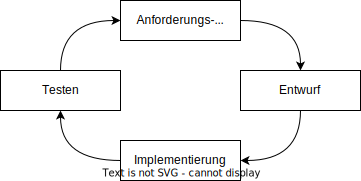
\includegraphics[scale=1.0]{Bilder/Kapitel-2/Abb-2-9.pdf}
	\caption[Iterative Softwareentwicklung]{Iterative Softwareentwicklung. Eine Iteration entspricht einem Zyklus in der Abbildung. Die mögliche zwischenzeitige Auslieferung von lauffähigen Versionen ist hier in der Abbildung nicht berücksichtigt.}
	\label{fig:iterative_softwareentwicklung}
\end{figure}

Durch die Entwicklung des Produkts als Folge von Iterationen kann das Entwicklungsteam von den gesammelten Erfahrungen während einer Iteration profitieren und damit nicht nur das Produkt, sondern auch die Arbeitsprozesse in den folgenden Iterationen optimieren. Im Unterschied zu sequentiellen Modellen, bei \mbox{denen} die verschiedenen Phasen (\zb Entwurf, Implementierung) sehr unter\-schied\-liche Arbeitsprozesse verlangen, sind sich die einzelnen Entwicklungsabschnitte eines iterativen Modells deutlich ähnlicher: die Prozesse des Softwareengineering werden in jeder Iteration erneut durchlaufen – wenn auch in einigen Vorgehensmodellen mit unterschiedlicher Schwerpunktsetzung. Somit können als ungünstig empfundene Arbeitsprozesse einer Iteration direkt in der nächsten Iteration verbessert werden. Ähnliches gilt übrigens auch für die eingesetzten Softwareentwicklungswerkzeuge  (\zb Entwicklungsumgebungen, Modellierungstools, Test-Frameworks). %\sttpgls{CASE_Tools}
Diese können in folgenden Iterationen gewechselt werden, wenn andere Werkzeuge geeigneter erscheinen. In sequentiellen Modellen können positive und negative Erfahrungen mit durchgeführten Arbeitsprozessen oder eingesetzten Werkzeugen dagegen erst im nächsten Softwareentwicklungsprojekt berücksichtigt werden.

\sttpHervorhebung{\textbf{In iterativen Modellen}}
\marginline{Einbezug Kunde}
\sttpHervorhebung{\textbf{wird der Kunde frühzeitig einbezogen.}}
Die Entwicklung in Iterationen erleichtert es, den Kunden in den Entwicklungsprozess einzubinden, zum Beispiel indem nach Abschluss jeder Iteration Rückmeldungen des Kunden eingeholt werden. Dabei besteht die Möglichkeit, anhand der aktuellen Version bzw. des aktuellen Stands Anforderungen für die nächste Version bzw. den nächsten Entwicklungsabschnitt zu verfeinern oder sogar neue Anforderungen zu spezifizieren. Gerade nicht technisch versierten Kunden fällt es sehr viel leichter, auf Grundlage schon funktionierender Software bzw. Prototypen Anforderungen oder Änderungswünsche zu äußern.
%\sttpgls{Prototyp} 

Um  Rückmeldung vom Kunden zu erhalten, kann die aktuelle Produktversion produktiv eingesetzt werden, der Kunde seine Erfahrungen sammeln und für die nächste Version kommunizieren. Rückmeldung kann aber auch heißen, dass die Version nur im Rahmen einer Produktvorstellung vom Kunden kommentiert wird und nicht produktiv eingesetzt wird. Bei letzterer Variante kann es sich dann um lauffähigen Code handeln – die Version somit potentiell produktiv einsetzbar sein – muss es aber nicht (\zb nur animierte Benutzungsschnittstellen). Für produktiv eingesetzte Versionen wird in der Literatur manchmal der Begriff \textit{Release}
\marginline{Release}
verwendet, der auch im Umfeld agiler Modelle verbreitet ist.

\pagebreak %%% für Druck

\sttpHervorhebung{\textbf{Iterative Modelle berücksichtigen Anforderungsänderungen.}} \marginline{Umgang mit Anforderungen}
Iterative Vorgehensmodelle können durch die kürzeren Entwicklungszyklen und die stärkere Einbindung des Kunden besser als inkrementelle Modelle und deutlich besser als sequentielle Modelle mit zusätzlichen oder veränderten Anforderungen während der Projektlaufzeit umgehen. Zudem tragen sie explizit der Tatsache Rechnung, dass es auch bei zu Projektbeginn feststehenden und stabilen Anforderungen aufgrund von Missverständnissen zwischen Kunden und Entwicklungsteam vorkommen kann, dass die Umsetzung nicht den (eigentlichen) Wünschen des Kunden entspricht. 

Iterative  Modelle sind daher gut geeignet, wenn die Funktionalitäten des zukünftigen Produkts zu Beginn der Entwicklung noch nicht komplett feststehen oder auf Änderungen während der Entwicklung reagiert werden soll. Letzteres bezieht sich im Übrigen nicht nur auf Änderungen der Anforderungen, sondern auch auf technologische Änderungen (\zb Verfügbarkeit passenderer Frameworks). Auf der anderen Seite besteht bei iterativen Modellen immer die Gefahr, dass die für die Kernversion gewählte Systemarchitektur sich in späteren Iterationen als zu unflexibel für den Einbau weiterer Funktionalität herausstellt und (aufwändig) überarbeitet werden muss. Diese Gefahr ist umso größer, je weniger klar der Kunde die Funktionalitäten des zukünftigen Softwareprodukts zu Projektbeginn spezifizieren kann. Wenn die fachlichen oder technologischen Unsicherheiten des Produkts zu Projektbeginn sehr groß sind, kann es sinnvoll sein iterative Modelle zusätzlich mit Verfahren aus dem Prototyping 
%\sttpkapitelverweis{Pro\-to\-typen\-ent\-wick\-lung}{Kap.~\ref{sec:Kap-7}}
zu verbinden. 

Aus Managementsicht liegt eine Schwierigkeit von iterativen Modellen in der Kontrolle des Projektfortschritts. Wenn zu Beginn des Entwicklungsprojekts nicht komplett feststeht, über welche Funktionalitäten das zu entwickelnde Produkt bei Fertigstellung verfügen wird, ist es während der Projektlaufzeit schwierig bis unmöglich zu beurteilen, ob der Entwicklungsfortschritt zu einem bestimmten Zeitpunkt im Zeitrahmen liegt oder nicht. Ebenfalls aufgrund der nicht vollständigen Spezifizierung der Anforderungen zu Projektbeginn ist auch die Vertragsgestaltung kompliziert, wenn ein Softwareprodukt nicht für das eigene Unternehmen, sondern für einen Auftraggeber entwickelt werden soll. Dieses Problem wurde in den 2000er Jahren mit dem stärkeren Einsatz agiler Vorgehensmodelle, bei denen die iterative Entwicklung essentieller Bestandteil ist, weithin sichtbar. Lösungsmöglichkeiten sind vorgeschaltete Prototyping-Projekte und neue Arten von Vertragsmodellen.

\sttpHervorhebung{\textbf{Iterative Modelle sind code- oder testorientiert.}} \marginline{Artefakte}
Codeorientiert bedeutet, dass am Abschluss jeder Iteration Programmcode steht. Iterative Modelle können (darüber hinaus) auch testorientiert sein, wenn Iterationen eine Menge zuvor spezifizierter Testfälle zugrunde liegen, die die jeweilige Produktversion der Software erfüllen soll. Basis für solche Testfälle können zum Beispiel typische Arbeitsabläufe sein, die die zukünftige Software unterstützen soll. 
%\sttpkapitelverweis{Use Cases}{Kap.~\ref{sec:Kap-6.2.1.1}}
%\sttpkapitelverweis{User Stories}{Kap.~\ref{sec:Kap-6.2.1.2}}

Anders als bei sequentiellen Modellen entstehen bei iterativen Modellen aufgrund der Verschmelzung der Softwareengineering-Prozesse und der starken Codeorientierung nicht automatisch während des Entwicklungsprozesses (Meilenstein)-Dokumente, wie eine strukturierte Auflistung der Anforderungen, eine Übersicht über alle Komponenten der Software, eine detaillierte Beschreibung einzelner Funktionen oder auch eine Historie getroffener Entwurfsentscheidungen etc. Eine Schwierigkeit iterativer Modelle besteht daher darin, wie das zukünftige Produkt und getroffene Entscheidungen dokumentiert werden. Eine entsprechende Dokumentation müsste parallel zur Implementierung innerhalb einer Iteration erstellt und bei Änderungen in späteren Iterationen immer wieder angepasst werden. Es ist stark abhängig vom konkreten Softwareentwicklungsprojekt, wie weitreichend eine Dokumentation des Systems und der getroffenen Entscheidungen in iterativen Modellen vorgenommen wird. Die minimale Variante ist der weitgehende Verzicht einer externen Dokumentation, indem der Programmcode möglichst „selbsterklärend“ gestaltet wird und nur um absolut notwendige Kommentare sowie um Funktionalitätsbeschreibungen von Schnitt\-stellen ergänzt wird. Weitergehendere Varianten wären die zusätzliche externe (und in späteren Iterationen jeweils anzupassende) Dokumentation der Anforderungen zum Beispiel anhand von User Stories oder die Dokumentation der Systemstruktur zum Beispiel anhand von Komponenten- und Klassendiagrammen. %\sttpkapitelverweis{Komponenten\-diagramme}{Kap.~\ref{sec:Kap-6.1.2}}
%\sttpkapitelverweis{Klassendiagramme}{Kap.~\ref{sec:Kap-3.2.4}} 
Weitreichende externe Dokumentationen dokumentieren darüber hinaus auch getroffene Entscheidungen und ihre Gründe – sei es klassisch in Form von Dokumenten oder agiler über Wikis oder Ticketsysteme –, um validere Folgeabschätzungen zu ermöglichen, falls getroffene Entscheidungen im späteren Projektverlauf revidiert werden müssen.

Das erste Vorgehensmodell, das umfangreichere Iterationen vorsah, war Ende der 1980er Jahre das Spiralmodell von Barry W. Boehm (\cite{boe86} und \cite{boe88}). Aus heutiger Sicht liegt die Bedeutung des Spiralmodells vor allem darin, dass es schon in den 1980er Jahren – und damit zur Hochzeit der phasenorientierten Modelle – ein iteratives Vorgehen und den Einsatz von Prototypen für die Entwicklung eines Softwareprodukts propagierte. Deutlich bekannter geworden ist aber der  im Zuge der objektorientierten Programmierung in den 1990er Jahren groß gewordene (Rational) Unified Process.

\sttpAutorenkasten{Barry W. Boehm}{1935}{2022}{
	\vspace{2mm} %%% für Druck
	US-amerikanischer Software\-ingenieur. Neben seiner Arbeit an Vorgehensmodellen ist er vor allem für das COCOMO-Modell bekannt. COCOMO (Constructive Cost Model) ist ein algorithmisches Modell, mit dem Kosten und Aufwand von geplanten Softwareprojekten geschätzt werden können.
	\vspace{2mm} %%% für Druck
}{Bilder/Autoren/boehm.jpg}{2006}{Improve it, \href{https://creativecommons.org/licenses/by-sa/2.0}{CC BY-SA 2.0}, via \href{https://commons.wikimedia.org/wiki/File:O_lend\%C3\%A1rio_Barry_Boehm.jpg}{Wikimedia Commons}}


\clearpage %%% für Druck

\subsubsection{Unified Process und Rational Unified Process}
\label{sec:Kap-2.2.2.1}

\vspace{\baselineskip} %%% für Druck

\sttpLeserfuehrung{Bilder/Kapitel-2/Leserfuehrung/vorgehensmodelle_iterativ_inkrementell_illustration.pdf}{Bilder/Kapitel-2/Leserfuehrung/vorgehensmodelle_rational_unified_process.pdf}

Ein  Kritikpunkt am Wasserfallmodell (und anderen Modellen der 1980er Jahre) war die starke Fokussierung auf rein softwaretechnische Aspekte und der damit niedrige Stellenwert der fachlichen Belange des Anwendungsbereichs des zu erstellenden Softwareprodukts. Das betraf den Einbezug zukünftiger Nutzer des Softwareprodukts ebenso wie den Umgang mit sich ändernden oder neuen Anforderungen aus der Domäne. Der Ende der 1990er Jahre im Zusammenhang mit der Unified Modelling Language (UML) entstandene und speziell auf objektorientierte Softwareentwicklung ausgerichtete Unified Software Development Process (kurz: Unified Process) \cite{jac99} legte den Fokus erstmals auf die Domäne und die Erfassung der dortigen Geschäftsprozesse. Der Unified Process selber ist ein sehr allgemein gehaltenes Vorgehensmodell, das zwar die Struktur des Vorgehens vorgibt, in den Details aber sehr unterschiedlich ausgestaltet werden kann. Von den verschiedenen Ausgestaltungen des Unified Process ist der Rational Unified Process die bekannteste Version.

Der von der Firma Rational Software (seit 2003 zu IBM gehörig) entwickelte Rational Unified Process (RUP) ist eine stark ausdifferenzierte und werkzeuggestützte Version des Unified Process. Er ist nicht nur ein Vorgehensmodell, sondern auch eine eigenständige Software-Suite, die verschiedene Entwicklungswerkzeuge anbietet, die auf Grundlage des Vorgehensmodells den Entwicklungsprozess eines konkreten Softwareentwicklungsprojekts unterstützen. 

\minisec{Struktur des Softwareentwicklungsprozesses}

Abbildung~\ref{fig:struktur_des_RUP} zeigt die Struktur des RUP. Der RUP unterscheidet die vier in der Abbildung in den Spalten dargestellten Phasen Konzeption (engl. inception), Ausarbeitung (elaboration), Konstruktion (construction) und Übergang in den Betrieb (transition), die nacheinander stattfinden. Jede Phase ist wiederum in Teilphasen (explizit \textit{Iterationen} \marginline{Iterationen}
genannt) aufgeteilt. Die Anzahl der Iterationen pro Phase ist nicht vorgegeben, sondern abhängig vom konkreten Softwareentwicklungsprojekt; die in der Abbildung dargestellte Anzahl der Iterationen daher nur beispielhaft. Im Gegensatz zu den Phasen eines Wasserfallmodells handelt es sich bei den RUP-Phasen nicht um die Prozesse des Softwareengineering, sondern um eine Aufteilung der Entwicklung in vier große Abschnitte, die jeweils mit Meilensteinen abgeschlossen werden und Auskunft über den Stand der Produktenwicklung geben. Die Prozesse des Softwareengineering bildet der RUP in sogenannten Disziplinen (engl. disciplines; in der Abbildung in den Zeilen dargestellt) ab. Hier werden die Prozesse Geschäftsprozessmodellierung (Business Modeling), Anforderungsermittlung (Requirements), Analyse und Entwurf (Analysis and Design), Implementierung (Implementation), Test (Test) und Auslieferung/Inbetriebnahme (Deployment) als sogenannte \textit{Kerndisziplinen}  sowie die \textit{unterstützenden Disziplinen} 
\marginline{Kerndisziplinen, unterstützende Disziplinen}
Konfigurations- und Änderungs\-manage\-ment (Configuration and Change Management), Projekt\-manage\-ment (Project Manage\-ment) und Entwicklungsinfrastruktur (Environment) unterschieden.

\vspace{-2mm} %%% für Druck

\begin{figure}[h!]
	\centering
	\includegraphics[width=\textwidth]{Bilder/Kapitel-2/StrukturRUP.pdf}
	\caption[Struktur des Rational Unified Process]{Struktur des Rational Unified Process, nach \cite[8]{shu08}}
	\label{fig:struktur_des_RUP}
\end{figure}

\vspace{-2mm} %%% für Druck

Der RUP adressiert mit den drei letztgenannten unterstützenden Disziplinen explizit auch diejenigen Aufgaben, die in einem Softwareentwicklungsprojekt außerhalb der reinen softwaretechnischen Prozesse durchzuführen sind. Innerhalb der Disziplin Projektmanagement nehmen dabei die Durchführung von Machbarkeitsstudien und Wirtschaftlichkeitsprüfungen, aber auch die Verwaltung von Risiko\-management\-plänen einen deutlich höheren Stellenwert ein als bei vielen anderen Vorgehensmodellen. Die Disziplin Entwicklungsinfrastruktur beinhaltet alle Aspekte, die die Bereitstellung von Hardware und Software für das Entwicklungsprojekt betreffen. Die Disziplin Konfigurations- und Änderungsmanagement beinhaltet Aufgaben, die sicherstellen, dass die im Projekt erstellten Dokumente verwaltet und ihre Konsistenz gewährleistet wird. Dazu gehört auch die Pflege einer Versionshistorie. 

In jeder Iteration sollen alle Disziplinen durchlaufen werden, allerdings mit verschiedener Schwerpunktsetzung. Dies verdeutlicht die Abbildung durch die unterschiedlich (und nur idealtypisch) verlaufenden Kurven in den Zeilen der Disziplinen. Je mehr Fläche unterhalb einer Kurve eingezeichnet ist, desto mehr Aufgaben aus dem Bereich der entsprechenden Disziplin werden während der jeweiligen Iteration durchgeführt. So haben zum Beispiel die Disziplinen Geschäftsprozessmodellierung und Anforderungsermittlung ihren Schwerpunkt in der Phase Konzeption, während die Implementierung hauptsächlich zum Ende der Ausarbeitung sowie während der Konstruktionsphase stattfindet. Im Vergleich zu Wasserfallmodellen ist somit nicht jeder Softwareengineering-Prozess fest zugeordnet, sondern wird in jeder Phase (wiederholt) durchlaufen. Insbesondere auch die bei Wasserfallmodellen kritisierte Ver\-ortung von Testaktivitäten löst der RUP dadurch besser. Eine gewisse Ähnlichkeit mit sequentiellen Vorgehensmodellen besteht allerdings doch, da die Schwerpunktsetzung der Kerndisziplinen in den Phasen der aus den sequentiellen Modellen bekannten Reihenfolge Anforderungsermittlung-""Entwurf-""Implementierung-""Testen folgt, auch wenn beim RUP grundsätzlich alle Disziplinen in allen Phasen aktiv sind. Auch Meilensteine am Ende von Phasen sind Charakteristika eines sequen\-tiel\-len Vorgehens, wobei die konkrete Ausgestaltung der Meilensteine im RUP (ausführbarer Architekturprototyp am Ende der zweiten Phase und Beta-Version des Softwareprodukts am Ende der dritten Phase) dann doch eher untypisch sind für sequentielles Vorgehen. 

\vspace{2mm} %%% für Druck

\minisec{Umgang mit Anforderungen}

Im  Vergleich zu vielen anderen Vorgehensmodellen werden im RUP zu Beginn eines Entwicklungsprojekts intensiv die durch das zu entwickelnde Softwareprodukt durchzuführenden oder zu unterstützenden Geschäftsprozesse der Domäne betrachtet. Innerhalb der Disziplin Geschäftsprozessmodellierung werden dafür mithilfe von Anwendungsfall\-mo\-dellen der UML %\sttpkapitelverweis{An\-wen\-dungs\-fall\-mo\-del\-le}{Kap.~\ref{sec:Kap-6.2.1}}
die relevanten Prozesse der Domäne dokumentiert oder auch spezifiziert, falls es sich um zu verändernde oder neu zu schaffende Geschäftsprozesse handelt. Das erfordert eine starke Einbindung der zukünftigen Nutzer des Softwareprodukts, da in der Regel nur diese die vertiefte Kenntnis über die Domäne besitzen. Die erstellten Anwendungsfallmodelle sind eine zentrale Grundlage für die Ermittlung bzw. zum Verständnis der funktionalen Anforderungen 
%\sttpkapitelverweis{funktionale Anforderungen}{Kap.~\ref{sec:Kap-6.1.3.2}}
des zu entwickelnden Softwareprodukts.

Im Rahmen der Disziplin Konfigurations- und Änderungsmanagement werden die Verfahrensweisen für den Umgang mit neuen oder sich ändernden Anforderungen während der Projektlaufzeit festgelegt. Der RUP ist deutlich flexibler bezüglich neuer Anforderungen als sequentielle Modelle, da über das definierte Änderungs\-management auch in späteren Projektphasen grundsätzlich noch Anforderungsänderungen möglich sind. Weitgehende Ergänzungen oder Änderungen der Anforderungen werden aber in der Regel erst in späteren Inkrementen bzw. Entwicklungszyklen berücksichtigt.

\vspace{2mm} %%% für Druck

\minisec{Artefakte des Entwicklungsprozesses}

Der RUP legt sehr detailliert fest, welche Aufgaben im Rahmen der Disziplinen auszuführen sind. Dafür definiert er zahlreiche verschiedene Rollen und Artefakte und spezifiziert detaillierte Prozessbeschreibungen, die Auskunft darüber geben, welche Aktivitäten durch welche Rollen zu welchen Zeitpunkten im Rahmen der Arbeitsabläufe welche Ergebnisse produzieren. Damit ist der RUP ein sehr detaillierendes Vorgehensmodell, das vor Projektstart an die spezifischen Bedürfnisse des konkreten Softwareentwicklungsprojekts angepasst werden muss (Tailoring, von engl. to tailor sth. = etwas maßschneidern). Diese Anpassung wird durch die Werkzeuge der RUP-Software unterstützt.

Den RUP kann man aufgrund des hohen Stellenwerts der geschäftlichen Anwendungsfälle als anwendungsfallorientiert bezeichnen, auch wenn ähnlich wie bei sequentiellen Modellen viele Artefakte des Entwicklungsprozesses Dokumente sind und somit die Bezeichnung dokumentenorientiert auch nicht falsch wäre.

\vspace{2mm} %%% für Druck

\minisec{Einordnung des RUP}

\vspace{1mm} %%% für Druck

Trotz der durchaus vorhandenen sequentiellen Charakteristika kann man den RUP in die Kategorie iterativ-inkrementelles Vorgehensmodell einordnen: Der wiederholte Durchlauf der Prozesse des Softwareengineering entspricht einem iterativen Vorgehen, auch wenn sich die Schwerpunktsetzung der einzelnen Iterationen unterscheidet. Die Bezeichnung iterativ bezieht sich aber auch darauf, dass komplette Entwicklungszyklen, also die Gesamtfolge der Phasen Konzeption-Ausarbeitung-Konstruktion-Übergang in den Betrieb wiederholt werden. Auf die Auslieferung der ersten Produktversion an den Kunden am Ende der Übergangs-Phase kann eine zweite Konzeptionsphase folgen und damit ein zweiter Entwicklungszyklus für die nächste Produktversion beginnen, die die erste Produktversion ersetzt. Der erste Entwicklungszyklus wird im RUP als \textit{Initialzyklus}, 
\marginline{Initialzyklus, Evolutions\-zyklen} 
die weiteren als \textit{Evolutionszyklen} bezeichnet. Diese Form von Iteration ist der Vorstellung von Iteration, wie sie im Rahmen der agilen Modelle verwendet wird, schon sehr nah. Bei der Wiederholung ganzer Entwicklungszyklen kann es sich statt um iterative aber auch um (klassisch) inkrementelle Entwicklung handeln, sofern die Produktversionen der Entwicklungszyklen eigenständige Teilprodukte bilden und durch spätere Inkremente ergänzt, aber nicht abgelöst werden. Im Falle von inkrementeller Entwicklung ist zudem die parallele Durchführung mehrerer Entwicklungszyklen möglich.

Der RUP definiert neben konkreten Arbeitspaketen grundlegende Prinzipien für die geschäftsprozessorientierte Softwareentwicklung, die aus in der Praxis bewährten Vorgehensweisen und Erfahrungswerten (\textit{Best Practices}) 
\marginline{Best Practices}
hervorgegangen sind. Solche prozessübergreifenden Grundsätze sind häufig auch essentieller Bestandteil agiler Vorgehensmodelle. Neben der Betonung der Wichtigkeit eines kontrollierten Anforderungs- und Änderungsmanagements gehört zu den Grundsätzen des RUP die schon erwähnte iterative anstelle der sequentiellen Entwicklung. Ein weiterer Grundsatz lautet, eine komponentenbasierte Architektur zu entwerfen, um so neben dem projektspezifischen Programmcode auch vorhandene Softwarekomponenten in das zu entwickelnde Softwareprodukt einzubinden. Einen hohen Stellenwert bekommen zudem die grafischen UML-Modelle zugeschrieben, und zwar nicht nur für Zwecke innerhalb des Entwicklungsteams, sondern vor allem auch zur Kommunikation mit Auftraggebern und Nutzern. Die starke Einbeziehung von Nutzern und die komponentenbasierte Entwicklung sind ebenfalls Aspekte, die man auch in agilen Vorgehensmodellen findet.

Seiner Entstehungszeit – zwischen vorherrschenden sequentiellen Modellen und aufkommenden agilen Strömungen – ist es vermutlich geschuldet, dass der RUP neben den ihm eigenen iterativen und inkrementellen Elementen einerseits Charakteristika sequentieller Vorgehensmodelle, andererseits aber auch solche späterer agiler Modelle aufweist. Trotz der agilen Elemente bleibt der RUP aber ein eher 
\marginline{schwer\-gewichtiges Modell}
schwergewichtiges Modell, das während des Softwareentwicklungsprozesses die Erstellung und Pflege zahlreicher Dokumente vorsieht, die später nicht direkter Bestandteil des Softwareprodukts werden. Dies ist die Stelle, an der sich der RUP am deutlichsten von agilen Vorgehensmodellen unterscheidet.
\subsection{Agile Modelle}
\label{sec:Kap-2.2.3}

\sttpLeserfuehrung{Bilder/Kapitel-2/Leserfuehrung/vorgehensmodelle_agile_illustration.pdf}{Bilder/Kapitel-2/Leserfuehrung/vorgehensmodelle_agile.pdf}

In den 1990er Jahren entstanden als Gegenbewegung zu den als schwergewichtig empfundenen vorherrschenden Softwareentwicklungsprozessen, die sich durch stark vorgegebene Abläufe und dokumentenorientierte Vorgehensweisen auszeichneten, sogenannte \textit{leichtgewichtige Modelle}. \marginline{leichtgewichtige Modelle}
Die Befürworter leichtgewichtiger Prozesse argumentierten, dass im Mittelpunkt von Softwareentwicklungsprojekten die Erstellung funktionierender Software und nicht die Abarbeitung von Regeln und das Produzieren von Dokumenten stehen müsse. Dementsprechend plädierten sie für eine Verschlankung und Flexibilisierung der Softwareentwicklungsprozesse. Basierend auf dieser Grundidee entwickelten sich Mitte bis Ende der 1990er Jahre die ersten leichtgewichtigen Vorgehensmodelle – wobei in diesem Kontext der Begriff 
\marginline{Entwicklungs\-modell}
\textit{Entwicklungsmodell} üblicher ist als Vorgehensmodell.

Die Bezeichnung \textbf{agil} für die leichtgewichtigen Modelle entstand, als sich im Februar 2001 in Utah, USA siebzehn Vertreter verschiedener leichtgewichtiger Modelle zu einem Gedankenaustausch versammelten, um Gemeinsamkeiten zwischen den verschiedenen Ansätzen zu finden. Alistair Cockburn, einer der Teilnehmer des Treffens, schrieb im Rückblick, dass der Begriff \textbf{leichtgewichtig} für viele Teilnehmer „eher eine Abneigung gegen etwas vermittelte als Vertrauen in etwas“ \cite[281]{coc03} und daher mit \textbf{agil} ein neuer Begriff gewählt wurde. Mit dieser Begriffswahl sollte zudem hervorgehoben werden, dass man im Laufe eines Softwareentwicklungsprojekts auf Veränderungen reagieren können muss. 

\sttpseitenrandzitat{„After a while we settled on Agile Software Development. Of course organizations would want to be agile. You can explain that to your CEO or customer far more easily than proclaiming you are extreme.“ \cite[16]{hun11}}{James Grenning, einer der Autoren des Agilen Manifests über die Wahl des Begriffs agil für Entwicklungsmethoden, die man bis dahin mit dem Extreme Programming verband.}

Auf  dem Treffen in Utah wurde als gemeinsame Erklärung das sogenannte 
\marginline{das Agile Manifest}
\textit{Agile Manifest} (Abb.~\ref{fig:das_agile_manifest}) verabschiedet. Es beinhaltet die grundlegende Philosophie der agilen Softwareentwicklung in Form von vier als \textit{Werte} bezeichneten Gegenüber\-stellungen. Wichtig ist, dass in diesem Manifest zwar eindeutige Präferenzen für die Aspekte in den ersten Satzhälften (\zb „Reagieren auf Veränderung“) zum Ausdruck gebracht werden, den Aspekten der zweiten Satzhälften (\zb „Befolgen eines Plans“), die dem Umfeld der schwergewichtigen Prozesse entstammen, aber ebenfalls Bedeutung beigemessen wird. So bedeutet zum Beispiel die Priorisierung funktionierender Software nicht zwingend den Verzicht auf eine (auch umfassendere) Dokumentation. Zusätzlich zu den Werten des Manifests einigten sich die Teilnehmer auf zwölf sogenannte \textit{Prinzipien}\footnote{\href{https://agilemanifesto.org/iso/de/principles.html}{https://agilemanifesto.org/iso/de/principles.html}.}, \marginline{Werte, Prinzipien}
die in Form von Handlungsanweisungen detaillierter als die Werte die Basis agiler Softwareentwicklung erläutern.

\begin{figure}[h!]
    \centering
    \includegraphics[scale=0.5]{Bilder/Kapitel-2/ScreenshotAgilesManifest.png}
    \caption[Das Agile Manifest]{Das Agile Manifest\\ (Screenshot von \href{https://agilemanifesto.org/iso/en/manifesto.html}{https://agilemanifesto.org/iso/en/manifesto.html})}
    \label{fig:das_agile_manifest}
\end{figure}

Mit der Verabschiedung des Agilen Manifests erfuhren die nun agil genannten Modelle einen – im zustimmenden wie im ablehnenden Sinne – enormen Bedeutungszuwachs. Werte und Prinzipien des Agilen Manifests bilden heute den Rahmen, innerhalb dessen sich – durchaus auch sehr verschiedenartige – Modelle und einzelne Methoden agil nennen. 

Agile Modelle sind immer iterative Modelle – allerdings nicht umgekehrt. Die iterative Entwicklung, in der für jede Produktversion alle Prozesse des Softwareengineering wiederholt durchlaufen werden, ist essentieller Bestandteil agiler Softwareentwicklung. Gleichzeitig sind agile Modelle auch inkrementelle Modelle, da es sich (ab einem gewissen Zeitpunkt im Projekt) zumindest bei Teilen der ausgelieferten Funktionalitäten um fertige Inkremente handelt, die nicht in späteren Versionen überarbeitet werden sollen.

\sttpHervorhebung{\textbf{Agile Modelle}} 
\marginline{Auslieferung}
\sttpHervorhebung{\textbf{liefern kontinuierlich lauffähige Software aus.}} 
Von einer ausgelieferten Produktversion zur nächsten vergehen in der Regel maximal einige Wochen. Aufgrund der kurzen Entwicklungszyklen spielen in agilen Modellen automatisiertes Testen, Verwendung existierender Frameworks und Bibliotheken sowie Einsatz von Entwicklungswerkzeugen eine besonders große Rolle. Erste Ideen und Ansätze, (Teile einer) Software schon während ihres laufenden Entwicklungsprozesses produktiv einzusetzen, hatte es bereits zu den Hochzeiten der Phasenmodelle in den 1980er Jahren gegeben \cite[84-2]{fav14}, aber erst im Kontext der agilen Modelle reiften diese Ideen zu einem grundlegenden Entwicklungsprinzip.

\sttpHervorhebung{\textbf{In agilen Modellen}} 
\marginline{Umgang mit Anforderungen} 
\sttpHervorhebung{\textbf{sind Anforderungsänderungen inhärenter Bestandteil des Softwareentwicklungsprozesses.}} 
Fehlende bzw. stark eingeschränkte Möglichkeiten auf die Änderung von Anforderungen zu reagieren, betrachten die Vertreter agiler Softwareentwicklung als den Hauptgrund für das Scheitern von Softwareentwicklungsprojekten. In agilen Modellen werden zu Beginn eines Softwareentwicklungsprojekts daher in der Regel nur der grobe Produktumfang und die grundlegenden Funktionalitäten (explizit noch in wenig detaillierter Weise) festgelegt. Weitere zu Beginn bekannte Anforderungen werden nur gesammelt (\zb bei Scrum im sogenannten Product Backlog, bei Extreme Programming  in Form von User Stories), ohne Anspruch auf Vollständigkeit der Sammlung und auch ohne Anspruch da\-rauf, dass alle dort gesammelten Anforderungen im Laufe der Produktentwicklung tatsächlich umgesetzt werden. Jegliche Auswahl und detailliertere Spezifikation von umzusetzenden Anforderungen erfolgt erst kurz vor Beginn derjenigen Iteration, in der sie implementiert werden sollen. Dadurch ist es möglich neue Anforderungen, die vom Kunden als prioritär gegenüber schon vorhandenen Anforderungen angesehen werden, vorzuziehen. Die Entscheidung, welche Anforderungen in der jeweiligen Iteration umgesetzt werden, wird in enger Abstimmung zwischen Kunden und Entwicklungsteam getroffen. Diese Flexibilität bezüglich der Anforderungsermittlung und –änderung sehen agile Modelle in der Regel auch für die Softwarearchitektur und eingesetzte Technologien vor (\zb Wechsel der Datenbanktechnologie, Wechsel eingesetzter Frameworks, Änderung der User-Interface-Technologie, Änderung von Server-Client-Zuständigkeiten).

\sttpHervorhebung{\textbf{Agile Modelle}} 
\marginline{Einbezug Kunde}
\sttpHervorhebung{\textbf{binden den Kunden intensiv ein.}} 
Der Kunde wird mindestens immer dann benötigt, wenn die zu realisierenden Anforderungen für die nächste Iteration festgelegt werden oder wenn eine neue Produktversion vorliegt. In vielen agilen Modellen ist der Kunde auch über diese Zeitpunkte hinaus in das Entwicklungsteam eingebunden, zum Beispiel um Rückfragen zu Anforderungen zu beantworten oder um implementierte Funktionalitäten schon während der Iteration zu testen. Agile Modelle sehen zudem die intensive Einbeziehung von Fachexperten vor. Ein Prinzip des Agilen Manifests verlangt sogar: „Fachexperten und Entwickler müssen während des Projektes täglich zusammenarbeiten.“\footnote{\href{https://agilemanifesto.org/iso/de/principles.html}{https://agilemanifesto.org/iso/de/principles.html}}
Die Rolle des Fachexperten kann dabei der Auftraggeber übernehmen; häufig wird aber unterschiedliche Expertise zu verschiedenen Aspekten der Domäne benötigt, sodass zusätzliche Personen ganz oder zeitweise einbezogen werden. Agile Modelle versuchen so, die Trennung zwischen Anwenderwelt und Entwicklerwelt so weit wie möglich aufzuheben. Diese Art der Einbindung von Kunden und Fachexperten in die Produktentwicklung erfordert im Vergleich zu klassischen Vorgehensmodellen die Etablierung spezifischer Kommunikationsstrukturen. Darüber hinaus stellt sie sehr hohe Anforderungen an die Personalressourcen des Auftraggebers, insbesondere wenn die fachliche Expertise von Mitarbeitern aus verschiedenen Abteilungen benötigt wird.

\vspace{1mm} %%% für Druck

\sttpHervorhebung{\textbf{Agile Modelle}} 
\marginline{Artefakte} 
\sttpHervorhebung{\textbf{sind code- oder testorientiert.}} 
Zudem legen sie Wert auf Einfachheit: Funktionalitäten sollen in dem Umfang entworfen und implementiert werden, wie sie aktuell benötigt werden und nicht so umfassend, wie sie zu einem späteren Zeitpunkt benötigt werden könnten. Die Herausforderung besteht darin, den Programmcode trotzdem so flexibel zu halten, dass spätere Erweiterungen der Funktionalität möglich bleiben, ohne die bisher geleisteten Arbeiten komplett verwerfen zu müssen.

\vspace{1mm} %%% für Druck

Ein verbreiteter Irrtum ist, dass in agilen Softwareentwicklungsprojekten aufgrund der Codeorientierung grundsätzlich nicht dokumentiert würde. Richtig ist, dass agile Modelle einen größeren Spielraum bezüglich der Dokumentation als andere Modelle lassen, da sie weitgehend keine verpflichtend zu erstellenden Artefakte vorgeben. Zudem werden für die Dokumentation in agilen Modellen in vielen Fällen andere Formen verwendet als in dokumentenorientierten Vorgehensmodellen. Darüber hinaus hängt es aber vom jeweiligen Projekt ab, in welchem Ausmaß eine Dokumentation erfolgt. Architektur- und Klassendiagramme, die die Struktur eines Systems beschreiben, lassen sich sowohl in agilen als auch in vielen anderen Vorgehensmodellen finden. In agilen Projekten entstehen sie (annähernd) parallel zur Implementierung des Produkts, müssen dafür aber deutlich häufiger angepasst werden. Entwurfsentscheidungen werden in agilen Projekten üblicherweise nicht im Rahmen eines eigenen Entwurfsdokuments beschrieben, sondern verteilen sich auf einzelne Wiki-Einträge, Fotos von am Whiteboard diskutierten Entscheidungen, Ticketsystem-Einträge, Kommentare im Programmcode etc., denen gemeinsam ist, dass sie in der Regel für andere Zwecke als zur Dokumentation entstanden sind – die Dokumentation insofern nur ein Nebeneffekt ist. Beschreibungen von Schnittstellen werden üblicherweise über Javadoc oder Vergleichbares in anderen Programmiersprachen realisiert. Sofern vom Kunden umfangreichere Dokumentationen gewünscht werden, werden diese Dokumentationsanforderungen in der Regel genauso behandelt wie Anforderungen an den Funktionsumfang der Software. Das bedeutet, sie müssen für die Anforderungssammlung erfasst und priorisiert werden.

\vspace{1mm} %%% für Druck

\sttpHervorhebung{\textbf{Agile Modelle stellen das Entwicklungsteam in den Mittelpunkt des Softwareentwicklungsprozesses.}} 
Neben  den Änderungen auf Prozessebene ging es den Befürwortern agiler Softwareentwicklung von Beginn an auch um Veränderungen der Unternehmenskulturen und dabei in erster Linie um die Fokussierung auf den Mitarbeiter als Individuum anstelle auf seine Rolle als Entwickler, Architekt, Tester etc. in vorgegebenen Verfahrensabläufen. Die Tätigkeit des Programmierens wird als Handwerkskunst verstanden, die (den klassischen Modellen unterstellte) Sichtweise der Programmiertätigkeiten als industrieller Prozess abgelehnt. Dementsprechend betont die agile Softwareentwicklung die Notwendigkeit, ein Unternehmens-/Projektumfeld zu schaffen, in dem Entwicklungsteams selbstorganisiert, flexibel und kreativ agieren können. Einen hohen Stellenwert nimmt dabei die Kommunikation und Zusammenarbeit innerhalb des Teams ein. Agile Modelle gehen meist davon aus, dass das Team an einem Ort – im Idealfall sogar im selben Büro – versammelt ist, und so intensiv von informeller Kommunikation während des Entwicklungsprozesses profitiert werden kann. Viele agile Modelle definieren darüber hinaus feste Kommunikationsformate für den Austausch über fachliche, aber auch über arbeitsatmosphärische, Aspekte. 

Im Vergleich zu sequentieller Softwareentwicklung unterscheidet sich die Zusammensetzung des Entwicklungsteams: Die starke Trennung verschiedener Rollen (\zb Architekt, Tester) entfällt, was für die einzelnen Teammitglieder in der Regel bedeutet, dass sie grundsätzlich – gegebenenfalls mit interner oder externer Unterstützung – alle anfallenden Arbeiten während des Softwareentwicklungsprozesses übernehmen können müssen. Die englischsprachige Literatur zu agilen Vorgehensweisen spricht in diesem Zusammenhang von „generalizing specialists“ \cite[35]{amb11} und bezeichnet damit Personen, die in wenigen Bereichen (\zb Datenbankentwurf, Backend-Programmierung) Spezialisten sind und in allen anderen Bereichen der Softwareentwicklung, inklusive der relevanten domänenspezifischen und technologischen Aspekte, über ausreichend Grundlagenwissen und Lernbereitschaft verfügen, dass sie nach Schulung oder Einarbeitung entsprechende Arbeiten übernehmen können.

\minisec{Einordnung agiler Modelle}

Aus klassischer Managementsicht fehlt agiler Softwareentwicklung die Möglichkeit, den Fortschritt eines Projekts zu kontrollieren. Die Befürworter agiler Modelle entgegnen, dass die einzig vertrauenswürdige Fortschrittsanzeige eines Softwareentwicklungsprojekts funktionierende Software sein könne. Diese verkörpere die Gesamtheit der Ergebnisse der Anforderungsanalysen, Entwurfs- und Implementierungstätigkeiten und sei damit die einzige relevante Größe. Für die Anwendung klassischer Managementprozesse sind die Nicht-Definition des endgültigen Produktumfangs zu Projektbeginn, fehlende Meilensteine zur Einschätzung eines eventuellen Zeitverzugs und fehlende längerfristige Entwicklungspläne allerdings ein Problem. Letztendlich muss die Managementebene darauf vertrauen, dass das Entwicklungsteam seine Arbeit innerhalb des Zeit- und Kostenbudgets erfolgreich abschließen wird. Auf das Team bezogen erfordert agile Softwareentwicklung die Fähigkeit zur Selbstorganisation, inklusive der eigenständigen Arbeitsverteilung und Einschätzung, an welchen Stellen die Einbindung externer Experten benötigt wird. 

\sttpseitenrandzitat{„Errichte Projekte rund um motivierte Individuen. Gib ihnen das Umfeld und die Unterstützung, die sie benötigen und vertraue darauf, dass sie die Aufgabe erledigen.“}{Eines der zwölf Prinzipien des Agilen Manifests \mbox{[\href{https://agilemanifesto.org/iso/de/principles.html}{https://agilemanifesto.org/iso/de/principles.html}]}}

Noch schwieriger als Controllingprozesse sind bei agiler Softwareentwicklung die Gestaltung der Verträge mit den Auftraggebern. Eingesetzt werden zum Beispiel vorgeschaltete Prototyping-Projekte, vorgeschaltete Projekte zur Erhebung von Geschäftsprozessen oder zentraler Anforderungen, die Auftragsvergabe anhand von Tagessätzen anstelle fest definierter Produktfunktionalität und spezifisch auf agile Projekte ausgerichtete Vertragsmodelle wie der „agile Festpreis“ \cite{ope18}, ein Vertragsmodell, bei dem zunächst nur ein Festpreisrahmen zwischen Auftraggeber und Auftragnehmer vereinbart wird.

Trotz Aspekten wie Selbstorganisation und Flexibilisierung von Prozessen sind agile Modelle keineswegs regellos. Die Vorgaben zur Sicherstellung qualitativ hochwertiger Entwicklung betreffen nur andere Ebenen als in anderen Vorgehensmodellen. So enthalten agile Modelle kaum bis gar keine Regeln zu Prozessabläufen oder zu produzierenden Artefakten, dafür aber durchaus nicht wenige Regeln zu Kommunikationsflüssen und arbeitsbezogenem Verhalten (\zb „keinen Code einchecken, der nicht getestet ist“, „keine Funktionalität implementieren, die nicht Bestandteil der aktuellen Iteration ist“). 

Der Einsatz agiler Modelle eignet sich insbesondere dann, wenn:

\begin{itemize}
	\item es schwierig bis unmöglich ist, Anforderungen an das zu erstellende Softwareprodukt zu Beginn des Projekts zu ermitteln, 
	\item zu erwarten ist, dass sich (Prioritäten von) Anforderungen im Laufe der Projektlaufzeit verändern werden,
	\item für ein dem Entwicklungsteam weniger bekanntes oder sich schnell änderndes technologisches Umfeld entwickelt werden soll,
	\item bestimmte Funktionalitäten vom Kunden sehr schnell benötigt werden, während andere deutlich weniger zeitkritisch sind.
\end{itemize}

Die unterschiedlichen agilen Modelle setzen die Werte und Prinzipien des Agilen Manifests in verschiedener Art und Weise um. 
   
\sttpseitenrandzitat{„Wir waren uns darüber einig, dass wir über diese Punkte [die vier Werte und die zwölf Prinzipien] hinaus nicht weiter übereinstimmten.“ \cite[281]{coc03}}{Alistair Cockburn, einer der Autoren des Agilen Manifests, über dessen Entstehung.}
Eines der ersten agilen Vorgehensmodelle war Extreme Programming, das Ende der 1990er Jahre vorgestellt wurde und das nach der Veröffentlichung des Agilen Manifests einen noch größeren Bekanntheitsgrad erreichte. Zu den heute bekanntesten und in zahlreicher Literatur zitierten agilen Modelle gehört Scrum, das Mitte der 1990er Jahre entstanden ist.
\subsubsection{Extreme Programming (XP)}
\label{sec:Kap-2.2.3.1}

\sttpLeserfuehrung{Bilder/Kapitel-2/Leserfuehrung/vorgehensmodelle_agile_illustration.pdf}{Bilder/Kapitel-2/Leserfuehrung/vorgehensmodelle_extreme_programming.pdf}

Das von Kent  Beck, Ward Cunningham und Ron Jeffries entwickelte Extreme Programming (Abkürzung XP) war Ende der 1990er und Anfang der 2000er Jahre das einzige leichtgewichtige Modell mit einem größeren Bekanntheitsgrad. XP verzichtet vollständig auf langfristige Entwicklungspläne und weitgehend auf die Produktion von Artefakten, die nicht Programmcode sind. Stattdessen kombiniert es verschiedene von den Urhebern und anderen Entwicklern eingesetzte und für sinnvoll befundene (Programmier)Verfahren zu einem kleinen Satz von Techniken, die 
\marginline{Praktiken} 
\textit{Praktiken} genannt werden. Im Unterschied zu den Praktiken des Agilen Manifests, die teilweise etwas philosophisch gehalten sind, handelt es sich bei den XP-Praktiken um sehr konkrete Vorgaben, welche Techniken und Methoden das Entwicklungsteam einsetzen und wie es Arbeitsprozesse gestalten soll. 

\minisec{Struktur des Softwareentwicklungsprozesses}

Das oberste Ziel von XP ist die Produktion von lauffähigem Programmcode in kurzen Zeitintervallen. Ein Entwicklungszyklus, dessen Dauer maximal wenige Monate beträgt und an dessen Ende eine an den Kunden ausgelieferte Produktversion (in XP \textit{Release}
\marginline{Release, Iteration, Task}
genannt) steht, setzt sich aus mehreren \textit{Iterationen} mit einer Dauer zwischen ein und vier Wochen zusammen. Die kleinste Einheit innerhalb einer Iteration ist eine Programmieraufgabe (\textit{Task}), die in der Regel ein bis drei Tage, manchmal aber auch nur einige Stunden Arbeitszeit erfordert. Beim ersten Release eines Softwareentwicklungsprojekts nach XP-Vorgehen handelt es sich um das Kernsystem, das durch die folgenden Releases jeweils inkrementell erweitert wird.

XP fordert die ständige Anwesenheit mindestens eines Kundenvertreters, um mit dem Entwicklungsteam unmittelbar kommunizieren zu können. Zu Beginn jeder Iteration werden in enger Zusammenarbeit zwischen Entwicklungsteam und Kundenvertretern im sogenannten Planungsspiel (s.u.) die Anforderungen bestimmt, die in der jeweiligen Iteration umgesetzt werden sollen sowie die Programmieraufgaben festgelegt, die sich daraus ergeben, und auf sogenannten \textit{Taskcards} \marginline{Taskcard}
festgehalten. Eine Taskcard ist eine Art logische Karteikarte, die eine reale Karteikarte, aber zum Beispiel auch Notizen am Whiteboard, Einträge im Wiki oder Tickets in einem Ticketsystem sein kann. Im Laufe der Iteration werden die Taskcards von den Programmierern abgearbeitet. XP gibt vor, dass immer zuerst die Anforderungen umgesetzt werden müssen, die der Kunde mit höchster Priorität gewichtet hat, damit die zum geplanten Releasetermin eventuell nicht fertiggestellten Funktionalitäten von geringerer Bedeutung sind. 

\sttpKasten{\textbf{Die XP-Philosophie}

Kent Beck beschreibt die Idee hinter seinem Vorgehensmodell und das \mbox{„Extreme“} in Extreme Programming folgendermaßen \cite[XV]{bec03}:

\textit{„Wenn Code Reviews gut sind, dann begutachten wir den Code andauernd [...]\\
Wenn Testen gut ist, dann testet jeder andauernd [...], auch der Kunde [...]\\ 
%~[...]\\ % Hinweis: die Tilde ~ wird gebraucht, da die eckigen Klammern am Zeilenanfang sonst nicht korrekt dargestellt werden
Wenn kurze Iterationszeiten gut sind, dann machen wir sie wirklich kurz – Sekunden, Minuten und Stunden statt Wochen, Monate und Jahre [...]\\
Als ich XP zum ersten Mal formulierte, hatte ich das Bild von Reglern auf einem Steuerpult im Kopf. Jeder Regler war ein Verfahren, von dem ich aus Erfahrung wusste, dass es gut funktioniert. Ich wollte alle Regler auf 10 aufdrehen und sehen, was dann passieren würde. Überraschenderweise erwies sich dieses Paket von Verfahren als stabil, vorhersehbar und flexibel.“
}}

\minisec{XP-Praktiken}
Ein Grundkonzept von XP ist die Methode der \textit{testgetriebenen Entwicklung} 
\marginline{Test-Driven Development}
(Test-Driven Development), die heute auch in viele andere (und durchaus nicht nur agile) Vorgehensmodelle Einzug gehalten hat – allerdings häufiger als Test-\textbf{First} statt Test-\textbf{Driven} Entwicklung.
%\sttpkapitelverweis{testgetriebene Entwicklung}{Kap.~\ref{sec:Kap-x.y}}
Bei der testgetriebenen Entwicklung  werden zunächst Testfälle für den zukünftigen Programmcode erstellt, bevor mit der Implementierung des Moduls begonnen wird. Im Rahmen von XP bezieht sich die testgetriebene Entwicklung nur auf die Ebene von Komponententests (engl. unit test; in Deutsch auch Modultest). 
%\sttpgls{Softwaretests} 
Die Komponententests können Fehler im Programmcode des entsprechenden Moduls finden, prüfen aber nicht, ob die Software die vom Kunden gewünschte Funktionalität aufweist. Dafür sieht XP Funktionstests (auch Akzeptanztests genannt) vor, die von den Kundenvertretern mit Unterstützung des Entwicklungsteams spezifiziert werden.

Die bekannteste mit XP in Verbindung gebrachte Praktik ist das Programmieren in Paaren (\textit{Pair Programming}). \marginline{Pair Programming}
%\sttpkapitelverweis{Pair Programming}{Kap.~\ref{sec:Kap-x.y}}
Dabei sitzen zwei Programmierer zusammen an einem Computer. Während einer programmiert, begutachtet der andere den Code und merkt direkt an, wenn ihm Probleme auffallen. Die Rollenaufteilung zwischen beiden Partnern kann flexibel wechseln. Pair  Programming umfasst nicht nur das reine Implementieren, sondern zum Beispiel auch die gemeinsame Arbeit an der Festlegung und Erstellung von Komponententests und die Diskussion über Lösungswege einer Programmieraufgabe. XP sieht vor, dass die Paarzusammensetzung häufig wechselt, durchaus auch mehrfach am Tag. 

Eng mit Pair Programming verknüpft ist in XP die Vorstellung eines 
\marginline{gemeinsames Codeeigentum}
gemeinsamen Codeeigentums: Jeder im Projekt erstellte Code „gehört“ allen Teammitgliedern und kann deshalb auch von jedem jederzeit verändert werden, wobei diejenigen, die Code ändern, dafür verantwortlich sind, dass dieser weiterhin die Testfälle erfüllt. Erforderlich dafür ist ein hohes Maß an Kommunikation zwischen den Programmierern und vor allem auch ein sehr ausgereiftes automatisiertes Versionsmanagement.
%\sttpkapitelverweis{Ver\-si\-ons\-ver\-wal\-tungs\-sys\-te\-me}{Kap.~\ref{sec:Kap-x.y}}
XP fordert zudem die Konzentration auf Einfachheit in der Implementierung: Jede Funktion soll nur genau so komplex implementiert werden, wie sie aktuell benötigt wird und nicht schon im Hinblick auf mögliche Erweiterungen ausgestaltet werden.

\sttpseitenrandzitat{„XP gleicht einer Wette. Man wettet darauf, dass es besser ist, heute etwas Einfaches zu tun und morgen etwas mehr zu zahlen, wenn man es ändern muss, statt heute etwas Kompliziertes zu tun, das vielleicht niemals eingesetzt wird.“ \cite[31]{bec03}}{Kent Beck}

Fertiggestellter Programmcode soll möglichst schnell in das Gesamtsystem integriert werden. Mindestens einmal am Tag, im Idealfall häufiger, soll daher jedes Programmierteam Code von seinem lokalen Computer in das System übernehmen. Dabei muss sichergestellt werden, dass definierte Integrationstests auch nach der Übernahme des eigenen Codes weiter fehlerfrei durchlaufen. Diese Vorgehensweise der kontinuierlichen Code\-inte\-gra\-tion (\textit{Continuous Integration}) \marginline{Continuous Integration}
%\sttpkapitelverweis{Continuous Integration}{Kap.~\ref{sec:Kap-x.y}}
ist wie Test-First Devel\-op\-ment eine Methode, die heute in vielen Softwareprojekten verwendet wird, unabhängig davon, ob sie mit XP als Entwicklungsmodell arbeiten oder nicht. 

Eine weitere zentrale Praktik in XP ist das sogenannte \textit{Refactoring}, \marginline{Refactoring}
%\sttpkapitelverweis{Refactoring}{Kap.~\ref{sec:Kap-x.y}} 
bei dem Änderungen am Programmcode vorgenommen werden, ohne dass sich das Verhalten (also die Funktionalität der Software) verändern soll. Refactoring zielt darauf ab, Aspekte wie Strukturiertheit, Verständlichkeit, aber auch Flexibilität des Programmcodes zu verbessern und damit die Qualität der Software zu erhöhen. Refactoring-Maßnahmen sind in XP explizite Arbeitsaufgaben in jeder Iteration. 

\vspace{1mm} %%% für Druck

\minisec{Umgang mit Anforderungen}

Die  Anforderungen an das zu entwickelnde Softwareprodukt werden in XP in Form sogenannter \textit{User Stories} \marginline{User Stories} spezifiziert, die die Kundenvertreter erstellen. User \mbox{Stories} beschreiben die Anforderungen an das zu erstellende System aus Sicht einer bestimmten Nutzergruppe, zum Beispiel über die Darstellung von Arbeitsprozessen, die die Software unterstützen soll (\zb „In meiner Rolle als Sachbearbeiter in der Personalverwaltung möchte ich die Gehaltsabrechnungen der Mitarbeiter verwalten“). Die User Stories sind Ausgangspunkt für das \textit{Planungsspiel}, \marginline{Planungsspiel} das zu Beginn jeder Iteration stattfindet und in dem versucht wird, die Kundenwünsche und die vorhandenen Entwicklungsressourcen einer Iteration in Einklang zu bringen. Dafür priorisieren die Kundenvertreter die User Stories und erläutern sie, sodass das Entwicklungsteam den Implementierungsaufwand abschätzen kann. Die Prioritäten kann der Kundenvertreter zu Beginn jeder Iteration (also auch noch innerhalb desselben Release-Zyklus) anpassen und auch neue Anforderungen hinzufügen. Gemeinsam wird anschließend die Dauer und der Umfang der Iteration festgelegt. Die vorgenommenen Aufwandsabschätzungen werden am Ende der Iteration mit den real investierten Aufwänden verglichen, um die Qualität der vorgenommenen Aufwandsabschätzungen im Projektverlauf stetig zu verbessern.

\vspace{1mm} %%% für Druck

\minisec{Artefakte des Entwicklungsprozesses}
XP gehört zu den agilen Modellen, in denen sehr wenig dokumentiert wird. Es setzt darauf, „dass mündliche Kommunikation, Tests und Quellcode die Struktur und den Zweck des Systems zum Ausdruck bringen.“ \cite[XVII]{bec03}. Dies betrifft auch die User Stories. Diese werden auf sogenannten Storycards nur sehr rudimentär beschrieben. XP gewichtet die direkte mündliche Kommunikation über die User Stories deutlich höher als deren schriftliche Fixierung. Durch die ständige Anwesenheit des Kundenvertreters kann das Entwicklungsteam auch jederzeit nach dem Planungsspiel Unklarheiten zur Umsetzung der User Stories mit diesem diskutieren. 

\vspace{1mm} %%% für Druck

\minisec{Einordnung von XP}
Eine entscheidende Rolle spielt bei XP die direkte (informelle) Kommunikation innerhalb des Entwicklungsteams. Dementsprechend eignet sich XP vor allem für kleine bis mittelgroße Teams („zwei bis zehn Programmierer“ \cite[XVIII]{bec03}), die eng zusammensitzen – im Idealfall im selben Büro – und gleiche Arbeitszeiten haben. 

Der geringe Grad an schriftlicher Dokumentation wird von XP-Kritikern als problematisch angesehen. Schwierig wird es vor allem dann, wenn mehrere Mitarbeiter das Softwareentwicklungsprojekt verlassen und damit zu viel Wissen über die Software verloren geht, das nicht dokumentiert ist. Das kann Gründe für Entwurfsentscheidungen betreffen, die neue Mitarbeiter nicht kennen, aber auch Priorisierungs\-entscheidungen zu noch umzusetzenden Anforderungen, die bei einem Wechsel des Kundenvertreters eventuell nicht mehr rekonstruierbar sind. Kompliziert kann es auch werden, wenn ein anderes Team die Wartung der Software übernehmen soll als das Team, das sie entwickelt hat. 

Ein weiterer Kritikpunkt an XP ist die unklare Beschreibung, wie der Aufbau einer Systemarchitektur gelingen soll. Einen expliziten Architekturentwurf sieht XP nicht vor. Letztendlich ist in einem konkreten Softwareentwicklungsprojekt entscheidend, dass das Entwicklungsteam genug Erfahrung im Aufbau von Softwarearchitekturen hat, um anhand einer Produktvision %\sttpkapitelverweis{Produktvision}{Kap.~\ref{sec:Kap-x.y}} 
die relevanten Leistungsmerkmale für die Erstellung der initialen Produktversion (erstes Release) bestimmen zu können.

Wie bei anderen agilen Modellen auch, lässt sich bei XP für Auftragsarbeiten die klassische Festpreis-Vertragsgestaltung zwischen Auftraggeber und Auftragnehmer nicht ohne Weiteres anwenden. Beck schlägt eine Art Abonnementmodell vor – wobei er allerdings nicht ins Detail geht –, bei dem Verträge über Laufzeiten und Kosten, aber nicht über feste Funktionalitäten geschlossen werden, die für den Auftraggeber auch wieder kündbar sind \cite[160]{bec03}. 

Ein Softwareentwicklungsprojekt, das nach dem XP-Entwicklungsmodell arbeiten möchte, muss nach Ansicht der XP-Urheber alle vorgesehenen XP-Praktiken anwenden, da diese sich gegenseitig stützen und in ihrem Zusammenspiel am gewinnbringendsten angewendet werden könnten. Das bedeutet aber nicht, dass man nicht einzelne Methoden auch gesondert einsetzen kann – nur entwickelt man dann halt nicht nach XP. Die Autoren von XP haben Praktiken wie Continuous Integration und Test-First Development, die man heute zu den grundlegenden Bestandteilen agiler Softwareentwicklung zählt, nicht erfunden; ihnen kommt aber sicherlich das Verdienst zu, sie weithin bekannt gemacht zu haben.

XP gibt, wie vorgestellt, viele Richtlinien für die konkreten Entwicklungsarbeiten vor, die vom Entwicklungsteam diszipliniert eingehalten werden müssen. Abgesehen von der Forderung, im Entwicklungsprojekt keine Überstunden notwendig werden zu lassen, legt XP aber nur wenige organisatorische Rahmenbedingungen fest. Das ebenfalls agile Vorgehensmodell Scrum geht den umgekehrten Weg.

\vspace{\baselineskip} %%% für Druck

\sttpseitenrandzitat{„Where XP has been responsible for much of the success of agile approaches within the IT \textbf{development} community, Scrum may be seen as being responsible for much of the success of agile approaches within the IT \textbf{management} community.“ \cite[84-10]{fav14}}{}

\clearpage %%% für Druck

\subsubsection{Scrum}
\label{sec:Kap-2.2.3.2}

\sttpLeserfuehrung{Bilder/Kapitel-2/Leserfuehrung/vorgehensmodelle_agile_illustration.pdf}{Bilder/Kapitel-2/Leserfuehrung/vorgehensmodelle_scrum.pdf}

Scrum ist ursprünglich für Managementprozesse in der Automobilindustrieproduktion entwickelt worden. Ken Schwaber und Jeff Sutherland  stellten es Mitte der 1990er Jahre erstmals für die Verwendung in der Softwareentwicklung vor. Zunächst war Scrum nur ein leichtgewichtiges Modell unter einigen anderen leichtgewichtigen Modellen. Seit Mitte der 2000er Jahre erhielt Scrum dann im breiten Bewusstsein immer mehr die Rolle als wichtigstes agiles Vorgehensmodell. Das hat vermutlich auch damit zu tun, dass man sich seit 2002 offiziell als Scrum Master (eine Rolle im Scrum Team) zertifizieren lassen kann. 

Scrum ist für kleine Teams mit üblicherweise weniger als 10 Personen \cite[5]{sch20} vorgesehen, für größere Projekte können mehrere Scrum-Teams gebildet werden. Scrum berücksichtigt deutlich stärker als XP die Projektmanagementsicht, indem es einen strikten organisatorischen Rahmen mit festen Kommunikationsformaten, Rollenzuständigkeiten und Kontrollmöglichkeiten des Projektfortschritts vorgibt. In Bezug auf konkrete Entwicklungsmethoden ist Scrum dagegen sehr viel flexibler als XP. Die Philosophie hinter Scrum lautet, dass das Entwicklungsteam selbstständig entscheidet, welche Entwicklungsmethoden und -werkzeuge es zur Erreichung seiner Ziele einsetzt. Eine Verbindung von Scrum mit XP-Methoden ist daher sehr gut möglich. 

\minisec{Struktur des Softwareentwicklungsprozesses}
Im  Vergleich mit XP verschwimmen bei Scrum die Grenzen zwischen iterativer und klassisch inkrementeller Entwicklung noch stärker. Während bei XP ein ausgeliefertes Inkrement (Release) in mehreren Iterationen entsteht, wird bei Scrum in jeder Iteration (in Scrum \textit{Sprint} genannt) \marginline{Sprint, Release}
eine lauffähige und (potenziell) vom Kunden einsetzbare Produktversion (ebenfalls \textit{Release} genannt) erzeugt, wobei bereits implementierte Funktionalität in folgenden Sprints wieder überarbeitet werden kann. Ein Sprint in Scrum sollte maximal einen Monat lang sein, in der Praxis üblich ist auch ein Zwei-Wochen-Rhythmus \cite[104]{kom17}. Die Sprint-Dauer für ein Projekt legt das Entwicklungsteam in Absprache mit dem Kunden fest. Wichtig ist dabei, dass alle Sprints des Entwicklungsprojekts gleich lang sein sollen und es somit nicht wie bei XP variable Zeitspannen für eine Iteration gibt. 

Scrum unterscheidet neben dem Entwicklungsteam nur die Rollen 
\marginline{Scrum Master}
\textit{Scrum Master} und Product Owner (s.u.). Der Scrum Master ist dafür zuständig, dass der Scrum-Prozess (insbesondere die vorgegebenen Kommunikations- und Kontrollformate) eingehalten wird. Zudem ist es seine Aufgabe, das Entwicklungsteam von äußeren Einflüssen (\zb Wünsche anderer Projekte oder der Managementebene der Firma) \mbox{abzuschirmen}, sodass das Team in seiner Produktivität nicht unnötig beeinträchtigt wird. Scrum kennt explizit keine Hierarchien im Scrum-Team. So soll insbesondere der Scrum Master nicht mit einem Entwicklungsleiter gleichgesetzt werden. Scrum schließt nicht aus, dass außerhalb der drei genannten Rollen noch weitere Personen am Entwicklungsprojekt beteiligt sein können, wie zum Beispiel Domänenexperten oder externe Berater. Diese gehören dann aber streng genommen nicht zum Scrum-Team.

Scrum  definiert vier feste Kommunikationsformate, die in jedem Sprint zwingend einzuhalten sind: Das Daily Scrum, das Sprint Planning und das Sprint Review (s.u.) sowie die Retrospektive. Das maximal 15-minütige \textit{Daily Scrum} \marginline{Daily Scrum} 
findet jeden Tag zur gleichen Zeit und am gleichen Ort statt. Dabei handelt es sich um ein Treffen des gesamten Teams, das im Stehen ausgeführt wird – eine Maßnahme, die helfen soll die veranschlagte Zeit einzuhalten – und in dem jedes Teammitglied die anderen über den aktuellen Stand seiner Arbeit, die Arbeitsplanung für den kommenden Tag und aufgetretene Probleme informiert. Auf diese Weise kann das Entwicklungsteam täglich seinen Projektfortschritt im Blick behalten.

Die Sprint \textit{Retrospektive} \marginline{Retrospektive}
findet am Ende eines Sprints statt. Die Retrospektive soll für das Scrum-Team die Gelegenheit bieten, „Wege zur Steigerung von Qualität und Effektivität zu planen.“ \cite[10]{sch20}. Hier geht es neben inhaltlichen und organisatorischen Aspekten der Prozessverbesserung vor allem auch um arbeitsatmosphärische (Un)Zufriedenheiten im vergangenen Sprint.

\vspace{-\baselineskip} %%% für Druck

\begin{figure}[h!]
	\centering
	\includegraphics[scale=0.7]{Bilder/Kapitel-2/ScrumProzess.png}
	\caption[Der Scrum-Prozess]{Der Scrum-Prozess \cite[7312]{gut15}}
	\label{fig:scrum_prozess}
\end{figure}

\minisec{Einbezug des Kunden}

Die \textit{Product Owner}-Rolle \marginline{Product Owner}
bei Scrum entspricht im Prinzip der Rolle des Kunden\-vertreters bei XP. Sofern mehrere Kundenvertreter ins Entwicklungsprojekt einbezogen sind, übernimmt einer von ihnen die Product Owner-Rolle. Der Product \mbox{Owner} spezifiziert und priorisiert die Anforderungen an das zu entwickelnde Software\-produkt sowie die zugehörigen Akzeptanztests.

\minisec{Umgang mit Anforderungen}

An Artefakten definiert Scrum neben dem Release nur das sogenannte 
\marginline{Product Backlog, Sprint Backlog}
\textit{Product Backlog} und das \textit{Sprint Backlog}. Das Product Backlog enthält die Anforderungen an das zu erstellende Softwareprodukt. Es wird vom Product Owner erstellt und kontinuierlich ergänzt, verändert und verfeinert, wobei der Product Owner gegebenenfalls von weiteren Domänenexperten oder vom Entwicklungsteam unterstützt wird. Die Verantwortung für das Product Backlog und die Priorisierung der darin enthaltenen Anforderungen (Product Backlog Items genannt) liegt immer beim Product Owner. Über das Product Backlog kann der Product Owner neue Anforderungen jederzeit einbringen, bestehende streichen oder verändern und somit im gesamten Verlauf des Entwicklungsprojekts flexibel Einfluss auf die Entwicklungsrichtung nehmen. 

Das Sprint Backlog enthält diejenigen Anforderungen des Product Backlog, die im aktuellen Sprint umgesetzt werden sollen. Spätestens wenn ein Backlog Item (eine definierte Anforderung) des Product Backlog in das Sprint Backlog aufgenommen wird, müssen Product Owner und Entwicklungsteam eine sogenannte \marginline{Definition of Done}
\textit{Definition of Done (DoD)}  
%\sttpkapitelverweis{Definition of Done}{Kap.~\ref{sec:Kap-x.y}}
für dieses Item erstellen. Eine DoD legt fest, welche Merkmale die Umsetzung einer Anforderung aufweisen muss, damit die Umsetzung als „fertig“ (heißt auslieferbar) gilt. Scrum macht keinerlei Vorgaben, wie eine DoD aussehen muss. Möglich wäre es zum Beispiel, die Erfüllung von bestimmten Akzeptanztests als Kriterium einer DoD anzusetzen.

Zu Beginn jedes Sprints legen Entwicklungsteam und Product Owner im 
\marginline{Sprint Planning} 
\textit{Sprint Planning} gemeinsam fest, welche der vom Product Owner mit höchster Priorität versehenen Product Backlog Items umgesetzt werden können. Spätestens dann müssen die einzelnen Items so detailliert spezifiziert sein (unter anderem durch die DoD), dass eine Aufwandsschätzung möglich ist. Es ist Aufgabe des Scrum Masters während des Sprints diese Aufwandsschätzung kontinuierlich mit dem real geleisteten Aufwand abzugleichen und zu kontrollieren, ob das Sprint-Ziel erreicht werden kann. Unter Umständen muss das Team in Absprache mit dem Product Owner den Leistungsumfang des Sprints reduzieren, indem bestimmte vorgesehene Items nicht umgesetzt werden. Ansonsten sind während eines Sprints keine Änderungen erlaubt. Auch neue Anforderungen, denen der Product Owner eine höhere Priorität zuteilt als den aktuell in der Umsetzung befindlichen, müssen bis zum nächsten Sprint warten, ein Tausch von Items ist nicht möglich. 

Dieses Einfrieren von Anforderungen während eines Sprints ist Scrums Lösung für den Spagat zwischen der Möglichkeit von Anforderungsänderungen und der Notwendigkeit von Planungssicherheit. Für Bertrand Meyer, der für sein 2014 erschienenes Buch „Agile! The Good, the Hype and the Ugly“ \cite{mey14} verschiedene agile Mo\-delle und Methoden analysiert hat, ist diese Scrum-Lösung die bedeutendste Idee des agilen Umfelds.

\vspace{3mm} %%% für Druck

\sttpzitat{„If out of my long immersion in agile methods for the preparation of this book I had to retain just one idea, that would be it. The principle is innovative, applicable, and effective.“ \cite[140]{mey14}}{Betrand Meyer über das Einfrieren von Anforderungen während eines Sprints}

\vspace{3mm} %%% für Druck

Im Kommunikationsformat des \textit{Sprint Review} \marginline{Sprint Review} begutachten und diskutieren Entwicklungsteam, Product Owner und eventuelle weitere Domänenexperten die Ergebnisse des Sprints (Umsetzung der Anforderungen). Daraus resultierende notwendige Änderungen oder neue Anforderungen werden ins Product Backlog eingetragen.

\minisec{Einordnung von Scrum}

Die von Scrum vorgegebenen Elemente sind fast ausschließlich auf der organisatorischen Ebene des Softwarenentwicklungsprojekts angesiedelt. Mit welchen Techniken die Ziele des Sprints erfüllt werden, wie die Aufgabenverteilung im Team aussieht, aber auch, in welcher Art und Weise die vorgegebenen Kommunikationsformate ausgestaltet werden, bleibt dem konkreten Team überlassen. Dieses ist damit in höchstem Maße (im positiven wie im negativen Sinne) eigenverantwortlich. In der Praxis werden insbesondere Teammitglieder, die schon in Scrum-Projekten gearbeitet haben, Ideen zu Prozessabläufen, Entwicklungsmethoden und -werkzeugen beisteuern können.

Wie für XP gilt auch für Scrum, dass es sich erst dann um einen Scrum-Prozess handelt, wenn \textbf{alle} Scrum-Regeln eingehalten werden. Nichtsdestotrotz lassen sich einzelne Scrum-Elemente auch in anderen Modellen verwenden. 

Im Gegensatz zu anderen agilen Modellen gibt es gegenüber Scrum wenige kritische Stimmen. Das hat sicher damit zu tun, dass Scrum keinerlei Vorgaben zu Entwicklungsmethoden macht und insofern, auch im Vergleich zu XP, deutlich weniger radikal wirkt. Theoretisch wäre es sogar möglich, innerhalb eines Sprints in einem wasserfallartigen Vorgehen zu arbeiten oder die einzelnen Product Backlog Items so detailliert schriftlich zu fixieren, dass eine umfassende Dokumentation der Anforderungen inklusive getroffener Entwurfsentscheidungen entsteht. In der Regel wird Scrum aber in Kombination mit agilen Methoden wie Test-First Development und Continuous Integration eingesetzt. Die Herausforderungen bezüglich der Vertragsgestaltung für Auftragsarbeiten und bezüglich vorhandener Unternehmensstrukturen (\zb Controllingabläufe, Berichtspflichten), die auf sequentielle Modelle ausgerichtet sind, teilt Scrum mit anderen agilen Modellen. 

% 2.3
\clearpage
\section{Vorgehensmodelle – Vergangenheit, Gegenwart und Zukunft}
\label{sec:Kap-2.3}

Wir haben uns 
\marginline{(Vor)Urteile}
in diesem Kapitel ausführlich mit Vorgehensmodellen im Softwareengineering befasst. Der eine oder die andere mag irritiert gewesen sein, dass auch die rückständigen sequentiellen Modelle Thema waren, die längst nicht mehr State of the Art sind, bei denen Menschen weniger zählen als Verfahrensabläufe und mit denen der Großteil der Softwareentwicklungsprojekte scheitert. Die eine oder der andere mag dagegen irritiert gewesen sein, dass auch die neumodischen agilen Modelle Thema waren, in denen chaotisch und ohne jegliche Rücksicht auf Budgets wild programmiert wird, die weder Anforderungen erheben noch Software dokumentieren und mit denen Softwareentwicklungsprojekte nie fertig werden.

\vspace{1mm} %%% für Druck

Solche und ähnliche (Vor)Urteile gegenüber der jeweils anderen Art von Vorgehensmodellen führten und führen seit dem Aufkommen der agilen Modelle Ende der 1990er Jahre zu heftigen ideologischen Verwerfungen zwischen Befürwortern und Gegnern agiler Softwareentwicklung. 

%%% Absatz hier für Druck
\vspace{1mm} %%% für Druck

Viele der frühen Verfechter agiler Modelle waren „Enthusiasten“ \cite[108]{som18}, die es als zwingend notwendig erachteten die bestehenden Software\-entwick\-lungs\-verfahren zu verwerfen und im gleichen Atemzug die gesamte Kultur der Soft\-ware\-entwick\-lung zu revolutionieren. Sie waren dementsprechend in keinerlei Hinsicht bereit, ihre agile Version auf bestehende Management\-verfahren und Unternehmens\-kulturen anzupassen oder gar einzuschränken. Die dadurch stark ideologisch geprägte Fundamentalkritik an den bestehenden Vorgehensmodellen erzeugte von deren Befürwortern als Gegenreaktion eine gleicherweise ideologisch geprägte Fundamentalkritik an sämtlichen Verfahrensweisen, die auch nur ansatzweise dem agilen Umfeld zugeordnet werden können. Insbesondere für die Vertreter eines sehr theoretisch orientierten Softwareengineering in Teilen der akademischen Welt (s. S.~\pageref{text:theoVertreter}) waren die agilen Methoden zudem ein ziemlicher Schock, denn sie negierten so ziemlich alles, was zur reinen Lehre der „guten“ Software\-entwicklung gehörte.

\vspace{1mm} %%% für Druck

Von den agilen Vorgehensmodellen war es vor allem XP, das kaum in bestehende Managementverfahren und Unternehmenskulturen passte – auch nicht passen wollte – und dementsprechend Gegenstand heftiger Diskussionen zwischen Befürwortern und Gegnern war. Besonders umstritten war die im Rahmen von XP vorgestellte Methode des Pair Programming, nicht nur aufgrund der offensichtlichen Frage, ob mit Pair Programming mehr oder weniger effizient Programmcode produziert werden kann als mit Einzelprogrammierung, sondern auch wegen der daraus folgenden kollektiven Verantwortung des Entwicklerteams für die Erstellung der Software und die Gewährleistung der Codequalität. Dieser Aspekt war mit den klassischen Vorstellungen von festen Zuständigkeiten und Verantwortlichkeiten einzelner Teammitglieder – insbesondere auch die Übernahme von Verantwortung für begangene Fehler – kaum vereinbar. 

%%% Absatz hier für Druck
\vspace{1mm} %%% für Druck

Es entstand eine Vielzahl von (teilweise wissenschaftlichen, nicht selten aber auch ideologisch angehauchten) Studien zum Pair Programming, allerdings mit so differierenden Ergebnissen, dass sich kein wirklich klares Bild über die Eignung oder Nicht-Eignung bzw. über messbare Vorteile des Pair Programming für die Softwareentwicklung erkennen lässt.\footnote{Wer dieses Thema vertiefen möchte, startet am besten mit den bei \cite[99]{som18} und \cite[232]{boe04} besprochenen Studien zum Pair Programming und nutzt dann deren Literaturangaben für die weitere Studiensuche.} 

\minisec{Bewertungen jenseits von Ideologien}
Es hat seit dem Aufkommen der agilen Modelle und Methoden relativ lange gedauert, bis man begann sich jenseits von ideologischen Betrachtungen der agilen Softwareentwicklung als Heiligem Gral oder achter Todsünde, auch differenzierter mit dem Sinn und Unsinn agiler Softwareentwicklung zu beschäftigen. Eine der ersten Gegenüberstellung von klassischer und agiler Softwareentwicklung lieferten im Jahr 2004 Barry Boehm und Richard Turner mit ihren Buch „Balancing Agility and Disci\-pline“ \cite{boe04}. Der Untertitel „A Guide for the Perplexed“ beschreibt den Fokus des Buchs: die Autoren stellen Kriterien auf, anhand derer konkrete Software\-entwicklungs\-projekte einen für sie gewinnbringenden Mix aus agilem und plangesteuertem – so der im Buch verwendete Begriff für die klassischen Vorgehensweisen – Vorgehen bestimmen können sollen. Anhand verschiedener organisatorischer, struktureller, personeller und technologischer Charakteristika von Softwareprojekten sowie deren Einsatzgebieten identifizieren die Autoren den jeweiligen „Home Ground“ der agilen und der plangesteuerten Softwareentwicklung. Der Begriff \textit{Home Ground} \marginline{Home Ground}
beschreibt dabei die Menge derjenigen Konstellationen von Projektcharakteristika, bei denen der Einsatz des entsprechenden Entwicklungsansatzes im Vergleich zum anderen Ansatz geeigneter ist. Insgesamt plädieren die Autoren aber dafür, nicht im Zustand des „single-method true believers“ \cite[22]{boe04} zu verharren, sondern sich pragmatisch derjenigen plangesteuerten und agilen Methoden zu bedienen, die für das konkrete Softwareentwicklungsprojekt passend erscheinen.

\vspace{3mm} %%% für Druck

\sttpzitat{„For plan-driven methods, that ground is generally large, complex systems, often with safety-critical or other high-reliability attributes. Requirements should be fairly \mbox{stable} and the environment somewhat predictable. Agile methods are more comfortable where the systems and development teams are smaller, the customer and users are readily available, and the requirements and environment are volatile.“ \cite[22]{boe04}}{}

\vspace{3mm} %%% für Druck

Eine analytische Darstellung und Bewertung von konkreten agilen Prinzipien, Rollen und Methoden der wichtigsten agilen Vorgehensmodelle (unter anderem XP und Scrum) lieferte 2014 das von Bertrand Meyer verfasste „Agile! The Good, the \mbox{Hype} and the Ugly“ \cite{mey14}. Sehr offen gegenüber innovativen agilen Konzepten und gleichzeitig sehr kritisch – und teilweise verbal schonungslos – gegenüber manchem Heilsversprechen der agilen Literatur ist dieses Buch die erste systematische wissenschaftliche Darstellung und Bewertung zentraler agiler Methoden und Vorgehensmodelle.

Heutige Lehrbücher zum Softwareengineering gehen recht unterschiedlich mit dem Thema agiler Softwareentwicklung um. Thematisiert wird sie mittlerweile eigentlich immer, aber die Spanne reicht von "`ja, das gibt es auch"' bis zu "`es hat bzw. wird die Softwareentwicklung revolutionieren"'. Ian Sommerville ist einen interessanten Weg gegangen, der auf die Home Ground-Vorstellung von Boehm und Turner passt. Sein Standardlehrbuch \cite{som18} zum Softwareengineering war erstmals 1980 erschienen und dementsprechend auf plangesteuerte Entwicklung ausgerichtet. Im Laufe der mittlerweile zehn Aktualisierungen des Lehrbuchs haben zwar auch agile Methoden ihren Stellenwert im Lehrbuch bekommen. Der rote Faden blieb aber die grundlegende Vorstellung eines von Beginn an systematisch vorgeplanten Softwareentwicklungsprozesses -- auch wenn in der neuesten Auflage die Prozesse des Entwurfs und der Implementierung an vielen Stellen (im Sinne der Vorstellung agiler Entwicklung) als deutlich verzahnte Prozesse dargestellt werden. Parallel erschien aber 2020 Sommervilles weiteres Lehrbuch "`Modernes Software-Engineering"' \cite{som20}, das den Fokus auf die Entwicklung kleinerer und mittlerer (nicht-sicherheitskritischer) Softwareprodukte für den freien Markt setzt. "`Schnelle Entwicklung und Lieferung sowie die Flexibilität, Änderungen schnell vorzunehmen, sind grundlegende Anforderungen an die Produktentwicklung."' \cite[34]{som20} Dementsprechend werden auch viele (ursprünglich) dem agilen Umfeld zugeschriebene Methoden in diesem Lehrbuch vorgestellt. 

\vspace{1mm} %%% für Druck

Die Diskussion, ob agile Softwareentwicklung grundsätzlich sinnvoll ist oder nicht, wird heute nicht mehr ganz so heftig geführt wie in den 1990er und 2000er Jahren, beendet ist sie jedoch nicht. Das hat sicher auch damit zu tun, dass verschiedene Menschen die Agilität oder Nicht-Agilität eines konkreten Software\-entwicklungs\-projekts sehr unterschiedlich bewerten würden. Die Prinzipien des Agilen Manifests sind eben Prinzipien und keine operationalisierbaren Kriterien, anhand derer man den Agilitätsgrad eines konkreten Softwareentwicklungsprojekts eindeutig bestimmen könnte. Andrew Hunt, einer der Autoren des Agilen Manifests hatte zum zehnjährigen Geburtstag des Manifests beschrieben, was Agilität für ihn bedeutet:

\vspace{3mm} %%% für Druck

\sttpzitat{„it’s not about doing pair programming, or having stand-up Scrum meetings. \mbox{Anyone} can dogmatically follow the practices prescribed by others. But true agility goes beyond the dogma, beyond the practices. Agility is about adapting; adapting your process, your language, your tools, your team, and yourself to respond to the situation at hand.” \cite[12]{hun11}}{}

\vspace{4mm} %%% für Druck

\minisec{Eingesetzte Vorgehensmodelle}
\phantomsection
\label{sec:Kap-2.3:heutigeVM}

\vspace{1mm} %%% für Druck

Zahlen zum Einsatz bestimmter (Kategorien von) Vorgehensmodelle(n) sind etwas mit Vorsicht zu behandeln. Manchmal sollen sie zeigen, dass sich ein bestimmtes Vorgehensmodell durchsetzt bzw. nicht durchsetzt. Manchmal wird versucht, ein realistisches Bild zu zeigen, doch ist die vorhandene Datengrundlage so klein, dass sich maximal für genau die befragten Projekte bestimmen lässt, welche Vorgehensmodelle eingesetzt werden. Hinzu kommt, dass auch mit methodischer Sorgfalt bei der Erhebung nicht verhindert werden kann, dass befragte Projekte eine abweichende Vorstellung von der Agilität bzw. Nicht-Agilität ihrer eingesetzten Methoden oder Modelle haben als die befragenden Wissenschaftler. Trotz dieser Einschränkungen möchten wir hier auf die Vorstellung von Zahlen zur Verbreitung von Vorgehens\-modellen nicht komplett verzichten.

Im Rahmen der zweiten Phase der internationalen HELENA\footnote{HELENA: Hybrid dEveLopmENt Approaches in software systems development. Im HELENA-Projekt untersuchen etwa 75 internationale Wissenschaftlerinnen und Wissenschaftler den Einsatz hybrider Methoden in der Softwareentwicklung. Zum Projekt und zugehörigen Publikationen \mbox{s.~\href{https://helenastudy.wordpress.com/}{https://helenastudy.wordpress.com/}}}-Studie \cite{kuh18} wurden Unternehmen gefragt, welche Softwareentwicklungsmodelle und -methoden sie einsetzen (s. Abb.~\ref{fig:softwareentwicklungsmodelle_und_methoden}). Bei den Antworten auf diese Frage finden sich im Jahr 2017 sowohl die agilen Modelle Scrum und XP als auch Wasserfallmodelle und andere Phasenmodelle.

\begin{figure}[h!]
    \centering
    \includegraphics[width=0.7\textwidth]{Bilder/Kapitel-2/VerteilungModelleMethoden.png}
    \caption[Eingesetzte Vorgehensmodelle und Methoden]{Eingesetzte Modelle und Methoden. Mehrfachnennung war möglich. \cite[10]{kuh18}}
    \label{fig:softwareentwicklungsmodelle_und_methoden}
\end{figure}

Die Studienreihe „Status Quo Agile“ der Hochschule Koblenz untersucht regelmäßig den Status Quo der Nutzung agiler Methoden. Für die Studie „Status Quo Agile – 3.~Studie zu Verbreitung und Nutzen agiler Methoden 2016/2017“ \cite{kom17} wurden etwa 1000 Unternehmen aus über 30~Ländern befragt, wobei aber 73\,\% der teilgenommenen Befragten aus Deutschland stammen. 

\pagebreak %%% für Druck

20\,\% der Befragten gaben an nur mit agilen Methoden zu arbeiten (s. Abb.~\ref{fig:einsatz_agiler_methoden}), während 12\,\% nur mit klassischen Methoden arbeiten. Das bedeutet, dass mehr als zwei Drittel der befragten Unternehmen entweder klassische und agile Methoden mixen (Kategorie Hybrid) oder bei einzelnen ausgewählten Prozessen agile Methoden einsetzen (Kategorie Selektiv). In der 4.~Studie der Reihe „Status Quo (Scaled) Agile 2019/20. 4.~Internationale Studie zu Nutzen und Erfolgsfaktoren (skalierter) agiler Ansätze“ \cite{kom20} hat sich im Jahr 2019 an diesem Befund nur wenig verändert. Der Anteil rein klassischer Methoden ist mit 9\,\% der Projekte etwas gesunken, der Anteil der durchgängig agilen Projekte liegt weiterhin bei 20\,\%, die hybriden Projekte konnten mit 43\,\% gegenüber dem nur selektiven Einsatz (28\,\%) etwas zulegen \cite[13]{kom20}.

\begin{figure}[h!]
    \centering
    \includegraphics[width=0.7\textwidth]{Bilder/Kapitel-2/EinsatzAgileMethoden.png}
    \caption[Einsatz agiler Methoden bei der Durchführung von Projekten]{Einsatz agiler Methoden bei der Durchführung und Planung von Projekten/Entwicklungsprozessen \cite[15]{kom17}}
    \label{fig:einsatz_agiler_methoden}
\end{figure}

Die Status Quo Agile-Studienreihe hat die Verbreitung agiler Methoden im Blick und fragte daher 2017 auch nach den Gründen, aus denen selektive bzw. hybride Formen – wie aus den vorgegebenen Antwortkategorien hervorgeht: an Stelle komplett agiler Formen – gewählt wurden (Abb.~\ref{fig:gruende_hybrid}). 

%%% Hier kommt Abbildung "fig:gruende_hybrid" eigentlich hin.

Auffällig ist hier, dass anscheinend häufig organisatorische Rahmenbedingungen und institutionelle Zwänge dem reinen agilen Vorgehen im Weg stehen. Vor diesem Hintergrund ist es nicht verwunderlich, dass ein agiles Modell wie Scrum, das deutlich managementfreundlicher als andere agile Modelle ist, sich gegenüber anderen agilen Modellen durchsetzen konnte. In der 4. Studie der Reihe wurde die Frage erneut – allerdings mit etwas abweichenden Antwortkategorien – gestellt \cite[24]{kom20}: Hauptgrund für die Nicht-Wahl eines reinen agilen Ansatzes bleiben die Rahmen\-bedin\-gungen (74\,\%). 

\pagebreak %%% für Druck

\begin{figure}[h!]
	\begin{addmargin*}[0cm]{-\marginparwidth}
		\begin{addmargin*}[0cm]{-\marginparsep}
			\centering
			\includegraphics[width=1.25\textwidth]{Bilder/Kapitel-2/GruendeHybrid.png}
			\caption[Gründe für eine selektive/hybride Form]{Gründe für eine selektive/hybride Form. Mehrfachnennung war möglich. \cite[29]{kom17}}
			\label{fig:gruende_hybrid}
		\end{addmargin*}
	\end{addmargin*}
\end{figure}

\begin{figure}[h!]
	\begin{addmargin*}[0cm]{-\marginparwidth}
		\begin{addmargin*}[0cm]{-\marginparsep}
			\centering
			\includegraphics[width=1.25\textwidth]{Bilder/Kapitel-2/GruendeKlassisch.png}
			\caption[Faktoren für die Wahl klassisch-plangetriebener Methoden]{Faktoren für die Wahl klassisch-plangetriebener Methoden. Mehrfachnennung war möglich. \cite[30]{kom20}}
			\label{fig:gruende_klassisch}
		\end{addmargin*}
	\end{addmargin*}
\end{figure}

\pagebreak %%% für Druck

Die 2019er-Studie fragt bei Projekten, die in die Kategorien Hybrid oder Selektiv fallen, außerdem nach den Gründen für die Wahl klassisch-plangetriebener statt agiler Methoden (Abb.~\ref{fig:gruende_klassisch}). Auch hier zeigt sich, dass für die Entscheidung zwischen agilen und plangetriebenen Methoden oft weniger einzelnen Methoden innewohnende Vor- oder Nachteile, sondern vielmehr die verschiedenen Umfeldfaktoren des Softwareentwicklungsprojekts eine Rolle spielen. 

%%% Hier kommt Abbildung "fig:gruende_klassisch" eigentlich hin.

Über Scrum sagen in der 2017er-Studie etwa 55\,\% derjenigen Befragten, die agile Methoden einsetzen, dass es eine zentrale Bedeutung in ihrem Tätigkeitsbereich habe und weitere etwa 25\,\%, dass es neben anderen Methoden in ihrem Tätigkeitsbereich genutzt werde \cite[50]{kom17}\footnote{die Frage lautete: „Welche Bedeutung haben die jeweiligen Methoden für Ihren Bereich?“. Die anderen beiden Antwortkategorien waren „geringe Bedeutung in meinem Tätigkeitsbereich“ und „keine Bedeutung für meinen Tätigkeitsbereich“, siehe \cite[50]{kom17}}. Damit führt Scrum eine Liste von 14 agilen Methoden an, für die die Studie die Bedeutung abfragt. XP liegt mit etwa 10\,\% für „zentrale Bedeutung“ und weiteren 20\,\% für „neben anderen Methoden genutzt“ in dieser Liste auf Platz~6.

Heute werden sie alle irgendwo eingesetzt – die sequentiellen Vorgehensmodelle, die agilen Vorgehensmodelle und vor allem die diversen Ausprägungen dazwischen! Manche Unternehmen versuchen eine gewisse Standardisierung zu erreichen und Projekte nach unternehmenseinheitlichen Vorgehensmodellen durchzuführen. Andere setzen je nach Projekt unterschiedliche Modelle ein. Es ist dabei sehr üblich die Grundform eines Vorgehensmodells spezifisch an das konkrete Projekt oder an übergeordnete Regeln des Unternehmens anzupassen. Die Status Quo Agile-Studie 2017 hat bei Projekten, die Scrum einsetzen, erhoben, inwieweit sich diese von den Vorgaben von Scrum entfernen und auf Grundlage von Scrum ihr eigenes unternehmens\-spezifisches Vorgehensmodell entwickeln: So setzen 11\,\% der Befragten Scrum ohne die Rolle des Scrum Master ein, in weiteren 19\,\% der Projekte agiert der Scrum Master eher wie ein (klassischer) Projektleiter, und 20\,\% der Projekte setzen einen Scrum Master und einen Projektleiter gleichzeitig ein \cite[99]{kom17}. Insofern halten sich nur die Hälfte der befragten Projekte an die in Scrum definierte Rollenausgestaltung des Scrum Master. Ein ähnliches Abweichen vom Grundmodell ist bei der Rolle des Product Owner zu beobachten: 13\,\% der Projekte haben gar keinen Product Owner bzw. lassen die Rolle von einem Mitglied des Entwicklungsteams übernehmen, und in 35\,\% der Projekte definiert der Product Owner die Sprint-Ziele \cite[100]{kom17}, obwohl Scrum hier explizit die gemeinsame Abstimmung zwischen Product Owner und Entwicklungsteam fordert.

\minisec{Fazit}

Sie haben im Laufe des Kapitels verschiedene Kriterien kennengelernt, anhand derer man Vorgehensmodelle unterscheiden kann. Die größten Unterschiede bestehen in den Strategien der Vorgehensmodelle mit neuen oder veränderten Anforderungen umzugehen. Warum ist das so? In einer idealen Welt, in der man für die Entwicklung eines Softwareprodukts unendlich viel Zeit und Geld hätte, alle Anforderungen unmissverständlich benennen könnte und wüsste, dass sich diese Anforderungen niemals ändern würden; in dieser Welt würde man zu Beginn eines Projekts alle Anforderungen detailliert aufschreiben, denn je umfänglicher man zu Beginn über die gewünschte Funktionalität Bescheid weiß, desto zielgerichteter und effizienter kann die Software entwickelt werden. Nur ist das leider unrealistisch. Daher muss jedes konkrete Softwareentwicklungsprojekt in irgendeiner Weise den Spagat schaffen notwendige Änderungen – im Übrigen nicht nur bezogen auf die Anforderungen – im Laufe des Projekts vornehmen zu können und gleichzeitig in der Lage sein das Zeit- und Kostenbudget möglichst einzuhalten, wofür in der Regel die Kontrolle des Projektfortschritts notwendig ist. Die verschiedenen Vorgehensmodelle verfolgen dafür unterschiedliche Strategien. Mit dem flexiblen Reagieren auf Änderungen haben sequentiell orientierte Entwicklungsprojekte die meisten Schwierigkeiten. Die Messung des Projektfortschritts stellt am häufigsten agile Projekte vor Probleme. Es ist daher nicht erstaunlich, dass verschiedene hybride Vorgehensmodelle publiziert werden, die versuchen – und in der Regel auch für sich in Anspruch nehmen es geschafft zu haben – die als sinnvoll erachteten Methoden aus klassischen und agilen Modellen optimal zu vereinen. Mit diesen hybriden Modellen werden wir uns nicht beschäftigen, da uns keines bekannt ist, das aktuell einen größeren Verbreitungsgrad erreicht hätte. Wie auch aus den oben gezeigten Grafiken deutlich wird, gestalten sich Unternehmen oder Projekte sowieso häufig ihre eigenen hybriden Modelle, indem sie zum Beispiel eigentlich agile Modelle um klassische Methoden zum Beispiel zu Projektplanung, Controlling oder Dokumentation erweitern oder in eigentlich sequentielle Modelle agile Elemente zum Beispiel für den Umgang mit Änderungen oder eine andere Art des Testens einbauen.\footnote{\cite{kuh19} werten auf Grundlage der HELENA-Daten \cite{kuh18} hybrides Vorgehen in europäischen Softwareentwicklungsprojekten aus. Der Artikel enthält eine Übersichtstabelle (S.~24~f.) mit Informationen, welche klassischen und welche agilen Methoden von den befragten Projekten kombiniert wurden.}

Ein noch immer heftig diskutiertes Thema im Kontext der Vorgehensmodelle ist die Skalierung von agilen Modellen. Agile Ansätze sind ursprünglich für kleine bis mittlere Teamgrößen gedacht, bei denen die Teammitglieder am selben Ort arbeiten. Diskutiert wird, ob und wie agile Ansätze auch für große und sehr große Entwicklungsteams oder regional verteilt arbeitende Teams sinnvoll eingesetzt werden können. Zu diesem Zweck wurden verschiedene Modelle publiziert. Drei der bekannteren sind das Scaled Agile Framework (SAFe) von Dean Leffingwell, das Agile Scaling Model (ASM) von Scott Ambler und Large-Scale Scrum (LeSS) von Bas Vodde and Craig Larman.\footnote{Weiterführende Informationen zur Skalierung agiler Ansätze und den genannten Modellen bei \cite[104 \psqq]{som18}, \cite[95 \psqq]{kom20} und \cite[41 \psqq]{amb11}.}

Im Umfeld der Vorgehensmodelle auch eher neu (etwa seit den 2010er Jahren) und doch gleichzeitig in gewisser Weise auch sehr alt – weil unter dem Aspekt Wartung schon in manchen sequentiellen Modellen vorhanden – ist die Ausweitung des Blickfelds der Softwareentwicklung in Richtung Softwarebetrieb. Dies ist insbesondere im Rahmen agiler Softwareentwicklung relevant, da Versionen der Software sehr häufig schon produktiv eingesetzt werden, während das Entwicklungsprojekt noch läuft und das Softwareprodukt kontinuierlich weiterentwickelt. Ansätze wie DevOps  
%\sttpkapitelverweis{DevOps}{Kap.~\ref{sec:Kap-x.y}}
betonen daher die Notwendigkeit, Prozesse der Softwareentwicklung und Prozesse des Softwarebetriebs viel enger miteinander zu verknüpfen – auch personaltechnisch. 

Jenseits der Fragen, ob Softwareentwicklung mehr oder weniger Prozesse benötigt, mehr oder weniger Dokumentationen zum Produkt erzeugen muss, sequentieller oder agiler erfolgen sollte; einer der wichtigsten Faktoren für eine erfolgreiche Software\-entwicklung bleibt das Entwicklungsteam. So mag oftmals die Wahl der Methoden und Vorgehensmodelle mehr von der Qualifikation der beteiligten Menschen abhängen als von den Charakteristika des Projekts. Die Vorgehensmodelle sind wichtig und hilfreich, aber mit einem unmotivierten Team entwickelt man mit jedem Vorgehensmodell schlechte Software - oder auch gar keine. Insofern gilt auch heute noch die mehr als dreißig Jahre alte Analyse von Watts Humphrey, der über viele Jahre einer der zentralen Akteure im Bereich der (klassischen) Software\-prozess\-verbesserung war: Es bedarf in jedem Softwareentwicklungsprojekt immer wieder der Abwägung zwischen dem „individual need for flexibility and the organizational need for standards and consistency“. Und dabei ist in jedem Fall zu berücksichtigen: 

\vspace{3mm} %%% für Druck

\sttpzitat{„Since software projects have differences, their software engineering processes must have differences as well. [...] In the absence of a universal software engineering process, organizations and projects must define processes that meet their own unique needs.“ Humphrey 1989, zitiert nach \cite[685]{sha11}}{}

\vspace{3mm} %%% für Druck

Letztendlich muss jedes Softwareentwicklungsprojekt für sich selbst herausfinden, nach welchem Vorgehen die Erstellung qualitativ hochwertiger Softwareprodukte in gegebenen Zeit-, Personal- und Kostenbudgets sowie bei gegebenen Rahmenbedingungen am besten gelingt.

% 2.4
% Kommentierte Literatur beginnt auf neuer Seite
\clearpage
\section{Kommentierte Literatur}
\label{sec:Kap-2.4}

%Bilder/Buchcover/Buchcover_SWEBOK.jpg
\sttpKommLitItem{Bourque/Fairley (Hrsg.)}{2014}{SWEBOK V3.0 – Kapitel 8}{swe14}{}{}
{Kapitel 8 „Software Engineering Process“ des SWEBOK, das Sie schon kennengelernt haben (s. S.~\pageref{sec:Kap-1.4:Bourque}), beschäftigt sich auch mit dem Thema der Vorgehensmodelle. Allerdings werden keine konkreten Vorgehensmodelle vorgestellt, sondern Kategorien von Vorgehensmodellen (sequentiell, inkrementell, iterativ, agil) gebildet und sehr knapp deren wichtigste Unterscheidungsmerkmale thematisiert. SWEBOK nimmt keinerlei Bewertung bezüglich der Überlegenheit oder Unterlegenheit im Vergleich der Vorgehensmodellkategorien vor. Stattdessen wird die Einzigartigkeit von Softwareentwicklungsprojekten und die daraus folgende Notwendigkeit betont, über eine individuelle Auswahl ein passendes Vorgehensmodell einzusetzen. Das Kapitel be\-inhal\-tet zudem Abschnitte zu organisationsbezogenen Softwareentwicklungsprozessen und entsprechenden Reifegradmodellen.}

%Bilder/Buchcover/Buchcover_Sommerville.jpg
\sttpKommLitItem{Sommerville}{2018}{Software Engineering}{som18}{}{}
{Kapitel 2.1 des aus der Einleitung (S.~\pageref{sec:Kap-0.3:Sommerville}) bekannten Lehrbuchs beschäftigt sich mit sequentiellen und in\-kre\-men\-tell-ite\-ra\-ti\-ven Vorgehensmodellen. Das Wasserfallmodell wird ausführlicher dargestellt, für RUP wird auf die Website zum Buch verwiesen. Die agile Softwareentwicklung bekommt in dieser 10. Auflage (engl. Auflage von 2015) ein eigenes Kapitel (Kapitel 3), in dem auch Scrum und XP thematisiert werden. Hervorzuheben sind hier eine gute Kurzzusammenfassung der wichtigsten XP-Praktiken (S. 92 f.) und ein Glossar der Scrum-Begriffe (S. 101) sowie ein eigenes Unterkapitel (Kap. 3.4) zur Skalierung agiler Methoden und der damit verbundenen Probleme. Insgesamt liegt der Schwerpunkt des Kapitels aber bei den heute relevanten agilen Methoden (unabhängig von ihrer Herkunft aus einem bestimmten Vorgehensmodell). Anhand der verschiedenen Auflagen des Lehrbuchs von Ian Sommerville lässt sich der Wandel von relevanten Themen im Softwareengineering beobachten, wie hier am Beispiel der Vorgehensmodelle: In der 9. Auflage des Lehrbuchs von 2011 lag der Schwerpunkt des Kapitels zu agiler Entwicklung noch beim konkreten Vorgehensmodell XP, während die vorhergehende 8. Auflage von 2007 die agile Softwareentwicklung noch gar nicht berücksichtigte, dafür aber ein längeres Unterkapitel zum RUP beinhaltete. Im 2020 erstmals erschienenen anderen Lehrbuch zum Thema Softwareengineering \cite{som20} vom selben Autor erhalten die Methoden der agilen Softwareentwicklung dann nochmal einen höheren Stellenwert.}

%Bilder/Buchcover/zeitung.png
\sttpKommLitItem{Royce}{1970}{Managing the Development of Large Software Systems}{roy70}{}{}
{Der Originalartikel zum ersten Wasserfallmodell [siehe auch Kap.~\ref{sec:Kap-2.2.1.1}]. Kurz und prägnant – zieht man die zahlreichen Abbildungen ab, verbleiben gerade mal \mbox{etwa} viereinhalb Seiten Text – erläutert Royce seine Vorstellung vom strukturierten Ablauf eines Softwareentwicklungsprojekts. Der Stil des Artikels ist sehr handlungsorientiert: viele Aussagen werden in Form von Faustregeln (engl. Howto) formuliert.}

%Bilder/Buchcover/Buchcover_Jacobson_Booch_Rumbaugh.jpg
\sttpKommLitItem{Jacobson/Booch/Rumbaugh}{1999}{The Unified Software Development \\ %%% für Druck
	Process}{jac99}{}{}
{Das Originalbuch zum Unified Process von dessen Erfindern. Der Unified Process verwendet für alle Prozesse als Modellierungssprache die UML, die von denselben Autoren entwickelt wurde. Das Buch stellt dementsprechend bei der Beschreibung der Bestandteile des Unified Process auch die UML vor. Aufbauend auf dem Unified Process sind verschiedene ausdifferenzierte (werkzeugunterstützte) Versionen entstanden, unter anderem der Rational Unified Process [siehe Kap.~\ref{sec:Kap-2.2.2.1} und \cite{kru99}].}

%Bilder/Buchcover/Buchcover_Kruchten.jpg
\sttpKommLitItem{Kruchten}{1999}{Der Rational Unified Process}{kru99}{}{}
{Originalbuch zum Rational Unified Process in deutscher Übersetzung. Das Buch beschreibt detailliert den Rational Unified Process sowie die zugrundeliegenden Best Practices, die der allgemeine Unified Process \cite{jac99} vorgestellt hatte.
}

%{Bilder/Buchcover/Buchcover_Marciniak.jpg}{S. 1804–1806}
\sttpKommLitItem{Alhir}{2002}{Unified Process}{alh02}{}{}
{Überblicksartikel aus einer Enzyklopädie des Softwareengineering zum Rational Unified Process (RUP). Der Artikel stellt den RUP, seine Charakteristika und Besonderheiten auf wenigen Seiten zusammenfassend dar. Er findet damit einen guten Mittelweg zwischen den oft zu verkürzten Darstellungen des RUP in Büchern oder Kapiteln zu Vorgehensmodellen und den vielen, bis ins kleinste Detail gehenden Darstellungen der exklusiv dem RUP gewidmeten Monographien. Der Titel des Artikels ist allerdings irreführend, da er sich nicht mit dem allgemeinen Unified Process, sondern mit der von Rational Software entwickelten Version beschäftigt.}

%Bilder/Buchcover/Buchcover_Beck.jpg
\sttpKommLitItem{Beck}{2003}{Extreme Programming: Das Manifest}{bec03}{}{}
{Die deutsche Übersetzung des Originalbuchs zu Extreme Programming von dessen Erfinder. Das Buch trägt den Untertitel „Das Manifest“ und dementsprechend ist auch die Art der Darstellung. Der Schwerpunkt liegt auf der Beschreibung von Zielen und Philosophie von XP. Die einzelnen Praktiken werden recht allgemein beschrieben oder anhand von einzelnen Anekdoten und Beispielen. Das Buch ist dementsprechend kein Nachschlagewerk, wie genau die Prinzipien von XP in konkreten Projekten angewendet werden können, sondern eher die Beschreibung einer umfassenderen Vision.}

%Bilder/Buchcover/Buchcover_Schwaber_Sutherland.png
\sttpKommLitItem{Schwaber/Sutherland}{2020}{Der Scrum Guide}{sch20}{}{}
{Etwa fünfzehnseitige Darstellung zu Scrums Regeln, Rollen und Artefakten von den Entwicklern von Scrum. Darstellungen zu Scrum findet man heute in zahlreicher Literatur, vielfach sind diese aber uneinheitlich oder sogar widersprüchlich. Da Scrum nur ein Rahmenwerk für agiles Projektmanagement ist und keine eigenen Entwicklungsmethoden (\zb in welcher Form wird getestet?, wie ist das Verhältnis zwischen Programmcode und Dokumentation?) anbietet, wird es in der praktischen Verwendung mit typischerweise agilen Entwicklungsmethoden (\zb Test-First Development) anderer Quellen kombiniert. In der Literatur zu Scrum vermischt sich dadurch häufig die Darstellung der eigentlichen Scrum-Inhalte mit der Darstellung der üblicherweise im Rahmen von Scrum-Projekten verwendeten Methoden. Der Scrum Guide ist das offizielle Scrum-Regelwerk, das bedeutet Regeln, Methoden oder Praktiken, die hier nicht aufgeführt werden, gehören auch nicht zu Scrum. Die Scrum-Autoren sind in dieser Hinsicht etwas puristisch. Sie weisen in einer Schluss\-bemerkung zum Guide zudem daraufhin, dass es sich nicht um eine Scrum-Entwicklung handelt, wenn man nur Teile von Scrum einsetzt. Dies ist, inklusive dem Abändern von Scrum-Regeln, in der Praxis aber durchaus üblich [siehe Kap.~\ref{sec:Kap-2.3}].}

%{Bilder/Buchcover/Buchcover_Gonzalez.jpg}{84-1 bis 84–28}
\sttpKommLitItem{Favaro}{2014}{Agile}{fav14}{}{}
{Dieser Artikel aus dem Softwareengineering-Handbuch \cite{gon14} stellt die Prinzipien des Agilen Manifests, daraus resultierende agile Methoden der Softwareentwicklung sowie konkrete agile Modelle – unter anderem XP und Scrum – vor. Unter einem recht weiten Blickwinkel werden dabei sowohl Vorläufer und Entstehungshintergrund einzelner Methoden, Gründe und Anlässe für ihre Aufnahme in den agilen Methodenkanon als auch die Konsequenzen ihres Einsatzes für die konkrete Ausgestaltung von Softwareentwicklungsprojekten dargestellt. Zudem stellt der Autor vor, welchen Weg – auch in nicht-agile Ansätze – die verschiedenen Methoden in der Softwareentwicklung seit der Veröffentlichung des Agilen Manifests genommen haben. Im zweiten Teil des Artikels gibt der Autor einen zusammenfassenden Überblick über Themen und Ergebnisse aktueller (2014) Forschungsfelder im agilen Umfeld. Der Artikel schließt mit einer umfangreichen Literaturliste und ist als Einstieg für die weitergehende Beschäftigung mit agilen Methoden und Modellen sehr zu empfehlen.}

\sttpKommLitItem{Sommerville}{2020}{Modernes Software-Engineering}{som20}{}{}
{Dieses Lehrbuch steht parallel zu dem regelmäßig aktualisiertem Standardlehrbuch zum Softwareengineering  \cite{som18} des Autors. Es verfolgt einen anderen Ansatz und setzt einen produktbezogenen anstelle eines projektbezogenen Fokus. Insbesondere geht es dabei mehr von Softwareentwicklungen für den Verkauf aus und weniger von einem Kunden, der eine Spezifikation vorgibt, aufgrund derer eine Softwarefirma ihm in einem Entwicklungsprojekt eine maßgeschneiderte Software erstellt. Das Buch beschäftigt sich sehr ausführlich mit agiler Softwareentwicklung und ihren wichtigsten Methoden.}

%{Bilder/Buchcover/Buchcover_Laplante.jpg}{S. 29–46}
\sttpKommLitItem{Ambler}{2011}{Agile Software Development}{amb11}{}{}
{Ein deutlich pro-agil gefärbter – der Autor ist ein überzeugter Vertreter und Entwickler agiler Methoden – aber nichtsdestotrotz sehr informativer Artikel über agile Softwareentwicklung. Der Artikel stellt verschiedene agile Praktiken vor und beschreibt, worin sich agile Ansätze von klassischen Softwareentwicklungsansätzen unterscheiden und worin sich beide Arten ähneln. Zielgruppe sind Projekte, die von anderen Vorgehensmodellen auf agile Vorgehensweisen wechseln möchten. Dafür beschäftigt sich der Artikel auch mit der Skalierung agiler Ansätze, die in der Regel für kleine und mittlere Teamgrößen konzipiert wurden, auf große und sehr große Entwicklungsteams.}

%/Bilder/Buchcover/Buchcover_Cockburn.jpg
\sttpKommLitItem{Cockburn}{2003}{Agile Software-Entwicklung}{coc03}{}{}
{Der Autor gehört zu den Begründern des Agilen Manifests und hat mit den sogenannten Chrystal-Family-Methoden auch selber ein agiles Vorgehensmodell vorgelegt, das in einem Kapitel dieses Buchs thematisiert wird. Der Schwerpunkt des Buchs liegt aber auf einer allgemeineren Beschreibung von Zielen, Philosophie und Methodik agiler Softwareentwicklung, insbesondere in den Bereichen Stellenwert von Individualität im Entwicklungsteam und Kommunikation. Ähnlich wie im Buch von Beck über XP \cite{bec03} geht es hier um die Darstellung einer Vision und weniger um Faktenwissen zu agilen Methoden. Sehr lesenswert ist das Kapitel über das Agile Manifest (S. 281ff), in dem aus einer Beteiligtenperspektive über Gründe und Zufälle für das Entstehen der Werte und Prinzipien des Manifests referiert wird.}

%/Bilder/Buchcover/zeitung.png
\sttpKommLitItem{Kneuper}{2017}{Sixty Years of Software Development Life Cycle Models}{kne17}{}{}
{Der Zeitschriftenartikel beschäftigt sich mit der Geschichte der Vorgehensmodelle seit den 1950er Jahren und stellt dabei auch die Verbindungen zwischen den Modellen (welches Modell ist aus welchem hervorgegangen) dar. Von den hier im Text betrachteten Vorgehensmodellen werden das Wasserfallmodell von Royce und der Rational Unified Process ausführlicher betrachtet. Die agilen Modelle werden nur allgemein behandelt. Dafür berücksichtigt der Artikel auch die frühen Modelle der 1950er und 1960er Jahre und stellt zum Beispiel das Modell von Benington, das wir im Zusammenhang mit dem Wasserfallmodell nur kurz erwähnt haben, detaillierter vor.}

%Bilder/Buchcover/Buchcover_Balzert.jpg
\sttpKommLitItem{Balzert}{2008}{Softwaremanagement}{bal08}{}{}
{Der dritte Band des dreibändigen Lehrbuchs zur Softwaretechnik beschäftigt sich mit Themen des Softwaremanagements. Einen großen Raum nimmt dabei der Abschnitt zu Vorgehensmodellen (unter dem Begriff Prozessmodell), Qualitätsmodellen und Reifegradmodellen ein (Kap. 16-24). Die Kategorisierung der Vorgehensmodelle unterscheidet sich von derjenigen von SWEBOK \cite{swe14}, die uns als Grundlage diente. Die hier im Text behandelten Vorgehensmodelle finden sich aber alle auch bei Balzert – entsprechend seiner Kategorisierung verteilt über verschiedene Kapitel.}

\sttpKommLitItem{Studienreihe Status Quo Agil – 3. Studie}{2017}{}{kom17}{}{}
{\href{https://www.gpm-ipma.de/wissen/studien/status-quo-agile}{https://www.gpm-ipma.de/wissen/studien/status-quo-agile}

Die Studienreihe „Status Quo Agile“ [siehe auch Kap.~\ref{sec:Kap-2.3}], wird vom „BPM-Labor für Business Process Management und Organizational Excellence“ der Hochschule Koblenz in Zusammenarbeit mit Scrum.org, GPM Deutsche Gesellschaft für Projektmanagement e.V. und teilweise weiteren wechselnden Partnern durchgeführt. Die Studienreihe erfragt seit 2012 alle paar Jahre in einer nicht-repräsentativen Studie die Nutzung agiler Methoden in Unternehmen. Schwerpunktmäßig werden Projekte der Softwareentwicklung oder anderer IT-naher Bereiche befragt, es finden sich aber auch Angaben aus IT-fernen Projekten. Etwa dreiviertel der Studienteilnehmer sind deutsche Unternehmen. Die einzelnen Studien der Reihe legen unterschiedliche Schwerpunkte, ein Großteil der Fragen bleibt aber ähnlich (teilweise veränderte Antwortkategorien).}

\sttpKommLitItem{Studienreihe Status Quo Agil – 4. Studie}{2019/20}{}{kom20}{}{}
{\href{https://www.gpm-ipma.de/wissen/studien/status-quo-agile}{https://www.gpm-ipma.de/wissen/studien/status-quo-agile}

Die Studie von 2020 setzt einen inhaltlichen Schwerpunkt auf den Themenbereich Skalierung agiler Ansätze  \cite[95 \psqq]{kom20}.}

%Bilder/Buchcover/zeitung.png
\sttpKommLitItem{Hunt et al.}{2011}{Agile @ 10}{hun11}{}{}
{Anlässlich des 10. Geburtstages des Agilen Manifests 2011 sendeten zehn der siebzehn Urheber ihre Gedanken zu den Fortschritten und Herausforderungen der agilen Softwareentwicklung für einen kurzen Zeitschriftenartikel einer Onlinezeitschrift ein. Die Beiträge der Autoren sind unterschiedlich lang und meist im Stil einer Kolumne gehalten. Sie beschreiben pointiert und sehr unterschiedlich enthusiastisch den Stellenwert der agilen Methoden innerhalb der Softwareentwicklung zehn Jahre nach der Veröffentlichung des Agilen Manifests.}

%Bilder/Buchcover/Buchcover_Boehm_Turner.jpg
\sttpKommLitItem{Boehm/Turner}{2004}{Balancing Agility and Discipline}{boe04}{}{}
{Eine sehr gute Gegenüberstellung zwischen plangesteuerter und agiler Softwareentwicklung bezüglich deren Charakteristika, Stärken und Schwächen, geeigneten Einsatzgebieten etc. [siehe auch Kap.~\ref{sec:Kap-2.3}]. Darüber hinaus werden ausführliche Fallbeispiele aus der Praxis vorgestellt, die die Grenzen von rein plangesteuertem und rein agilem Vorgehen aufzeigen sollen. In diesem Kontext sehr nett zu lesen ist auch die – natürlich entsprechend konstruierte – Fabel von Elefant (plangesteuerte Modelle) und Affe (agile Modelle), mit der die Autoren ihr Buch beginnen und die ihr Credo beinhaltet: Elefant und Affe sind erst dann erfolgreich, wenn sie die Stärken des jeweils anderen anerkennen und einen Weg gefunden haben, ihre Stärken zu verbinden. Die Autoren Barry Boehm (Wasserfallmodell, Spiralmodell) und Richard Turner (Reifegradmodell CMMI) verband man zur Entstehungszeit des Buchs (2004) eher mit plangesteuerter als mit agiler Softwareentwicklung. Die von Pragmatismus statt von Ideologie geleitete Herangehensweise der Autoren zeigt sich auch daran, dass Alistair Cockburn (einer der Autoren des Agilen Manifests) ein sehr positives Vorwort zum Buch verfasst hat.}

%Bilder/Buchcover/Buchcover_Meyer.jpg
\sttpKommLitItem{Meyer}{2014}{Agile! The Good, the Hype and the Ugly}{mey14}{}{}
{Der Autor Bertrand Meyer gehört zu den Großen in der Informatik: er hat wichtige Prinzipien der objektorientierten Softwareentwicklung entworfen, die Programmiersprache Eiffel erfunden und das in der Softwareentwicklung wichtige Konzept „Design by Contract“ entwickelt. Im Umfeld der agilen Softwareentwicklung war er bis zu diesem Buch weniger präsent. Das Buch stellt agile Prinzipien, Rollen und Methoden (unter anderem diejenigen von XP und Scrum) vor und bewertet sie hinsichtlich ihrer Vor- und Nachteile, ihrer Eignung für die praktische Softwareentwicklung und ihres Innovationspotenzials. Der Schwerpunkt des Buchs liegt auf der Bewertung der agilen Ansätze [siehe auch Kap.~\ref{sec:Kap-2.3}]. Die dafür notwendige Beschreibung der Ansätze ist in der Darstellungsart dabei teilweise stringenter und verständlicher als in vieler agiler Originalliteratur.}
\cleardoublepage
% Kapitel Fallbeispiel Zoo: über das Marko werden Kapitel, Eintrag Inhaltsverzeichnis und die Kopfzeilen konfiguriert.
\FallBeispielZoo
\label{sec:Lektion-1-Zoo}

Wir möchten hier am Ende dieser ersten Lektion mit einem Fallbeispiel beginnen, das Sie in den weiteren Lektionen immer mal wieder begleiten wird. Es dient dazu, aus einem praktischeren Blickwinkel ein paar Schlaglichter auf typische Tätigkeiten im Softwareengineering zu werfen. Die Simulation eines kompletten Software\-entwick\-lungs\-prozesses anhand eines Fallbeispiels ist im Rahmen einer solchen Lehrveranstaltung allerdings nicht möglich. Für das Fallbeispiel haben wir den Real\-weltbereich des Zoos gewählt und entschuldigen uns schon einmal im Vorfeld bei allen Zoo-Spezialistinnen und Zoo-Spezialisten für die Halbwahrheiten und erfundenen Informationen zur Lebenswelt Zoo in diesem natürlich für unsere Lehrzwecke so konstruierten Fallbeispiel.

\minisec{Die Ausgangslage}
Sie haben kürzlich Ihr Informatik- (wahlweise Wirtschaftsinformatik-) Studium abgeschlossen und Ihre erste Stelle in einem Unternehmen angetreten, das Softwarelösungen für kleine und mittelständische Betriebe entwickelt. Ihr neuer Chef, Herr Steiber, informiert Sie und Ihre Kolleg:innen über ein neues Projekt.

\textbf{Hr. Steiber:} „Was wissen Sie über Zoos? Wenig? Geht mir auch so. Aber das wird sich für uns alle wohl bald schon ändern: Einige von Ihnen kennen Frau Dr. Walther ja schon, die Direktorin des Zoos hier in der Stadt – und eine gute Bekannte von mir. Frau Dr. Walther ist vor einiger Zeit auf mich zugekommen, da der Zoo eine Zoo-Verwaltungssoftware benötigt. Nur, was genau gebraucht wird, in welchem Umfang, für welche Aufgaben usw. das scheint offensichtlich noch recht unklar zu sein. Frau Dr. Walther und einige ihrer Kolleginnen und Kollegen werden nächste Woche zu einem ersten Informationsgespräch bei uns vorbei kommen und ich möchte das gesamte Team bitten, dabei zu sein. Ich kann noch gar nicht einschätzen, in welchem Rahmen sich ein eventuelles Projekt bewegen würde und insofern müssen wir bei diesem ersten Gespräch auch herausfinden, inwiefern es sich für uns überhaupt lohnen würde, weitere Ressourcen zu investieren und auf eine Auftragserteilung hinzuarbeiten. Das zu lösende Problem darf einerseits natürlich nicht zu klein sein – ich sag mal, nur Eingabemasken zu erstellen, in der die Namen der Zootiere eingeben werden können, ist für uns nicht interessant. Auf der anderen Seite können wir mit unserem doch recht kleinen Team natürlich auch keine allumfassende Automatisierung sämtlicher Zooabläufe liefern - Ich fürchte ein wenig, dass es genau das ist, was der Zoo sich vorstellt. Wir werden sehen!“

\minisec{Beim ersten Treffen mit dem Zoo-Team}

\textbf{Fr. Walther (Zoodirektorin):} „Hallo. Schön, dass wir heute hier bei Ihnen sein dürfen. Herr Steiber hatte mich gebeten, etwas zu unserem Zoo zu sagen. Das ist kein Problem! Außerdem soll ich ja schon mal skizzieren, was die von uns gewünschte Zoo-Software können muss. Aber woher soll ich das wissen? Sie sind doch die Experten in der Softwareentwicklung. Sie wissen viel besser, was Softwareprodukte können müssen. Also, unser Zoo: Wir haben jährlich ca. 150.000 Besucher, im Jahresverlauf ist die Besucherzahl stark schwankend. 80 Prozent unserer Besucher sind Kinder. Natürlich hat irgendwie jedes Kind sein eigenes Lieblingstier, was sie aber alle auch mögen, ist unser Streichelzoo. Da haben wir nicht nur die üblichen Kaninchen, Meerschweinchen, Ziegen und Schafe, sondern auch unser Warzenschwein Rudi. Rudi war das erste Tier, für das wir vor ein paar Jahren die Möglichkeit eingerichtet haben, für einen jeweils begrenzten Zeitraum eine Patenschaft zu übernehmen. Mittlerweile existieren weitere Patenschaften für vier unserer Schlangen, unsere zwei Axolotl und den Kormoran. Eigentlich möchten wir das Patenschaftssystem auf alle unsere Tiere ausweiten und auch die Möglichkeit unterschiedlich langer Patenschaften bieten, aber ohne technische Unterstützung ist der Verwaltungsaufwand zu hoch. Kinder, die eine Patenschaft übernommen haben, erhalten für diesen Zeitraum freien Eintritt in den Zoo und können an bestimmten Tagen beim Füttern ihres Patentiers helfen. Wir beschäftigen fünfzehn Tierpflegerinnen und Tierpfleger und einen Tierarzt als Angestellte. Oft reicht ein Tierarzt nicht aus, sodass wir in diesen Fällen externe Tierärzte beauftragen müssen, was so kurzfristig oft nicht immer einfach ist. Wir planen langfristig eine zweite feste Tierarztstelle im Zoo einzurichten, vor allem da wir aktuell unseren Tierbestand erweitern. Bisher haben wir 26 verschiedene Tierarten mit entsprechend vielen Unterarten, \zb haben wir drei verschiedene Affenarten im Zoo. Natürlich hat jedes Tier einen Namen, und wir versuchen immer die Besucher einzubinden, wenn ein neugeborenes Tier einen Namen benötigt. Da kommt dann auch mal Shaggy raus als Name für unsere gestern geborene Testudo Graeca. Wir würden gerne alle Informationen zu unseren Tieren – also wann sie geboren sind, wer die Eltern sind, wie alt sie werden können, was sie fressen, aus welchem Zoo sie gegebenenfalls ausgeliehen sind und wie lange und ganz vieles mehr – unseren Besuchern auch über das Internet zur Verfügung stellen, aber das ist sicher aufwändig. Andererseits könnte man dann vielleicht die Eintrittskarten auch gleich online verkaufen, vielleicht würden wir dann noch mehr Besucher bekommen. Wir nutzen schon ein Onlinesystem, wenn wir Käfige oder Tiere aus anderen Zoos für eine bestimmte Zeit ausleihen und eine Software, mit der wir die Dienstpläne und Aufgaben unserer Tierpfleger verwalten, das wär schon gut, wenn das alles ein System wäre. Wir möchten langfristig nur noch fest installierte Gehege für die Tiere haben, in denen sie auch genug Platz und artgerechte Bedingungen haben, aber im Moment müssen wir auch Tiere in Käfigen halten, da sich die Bauarbeiten für die Zoo-Erweiterung verzögern. Aber wenn das mal fertig ist, werden wir endlich auch Eisbären und Nashörner haben, da fragen die Besucher nach. Seit letztem Jahr haben wir zwei Giraffen, da erhoffen wir uns dieses Jahr Nachwuchs. Tja, was müssen Sie noch wissen über unseren Zoo? Ja, genau: wir haben auch mehrere Spielplätze und natürlich Eis- und Pizzastände. Die Essensstände haben wir verpachtet. Das läuft ganz gut. Um das Essen für die Tiere kümmern sich die jeweiligen Tier\-pfleger, die kaufen entsprechend ein. Das müsste man sich auch mal angucken, ob es nicht sinnvoller wäre, die Futterbestellungen zentral zu machen, das müsste doch mit Softwareunterstützung auch viel leichter zu realisieren sein, und dann könnten wir vielleicht auch gleich noch für die Besucher im Internet Informationen über die Tierpfleger zur Verfügung stellen. Gerade unsere Stammgäste mit den Jahreskarten finden es wichtig den Tierpfleger zu kennen, der ihr Lieblingstier versorgt. Was meinen Sie, wie lange brauchen Sie für unsere Zoo-Software?“
	
	% Literaturverzeichnis für diese Lektion
	\cleardoublepage % auf einer neuen rechten Seite
	\printbibliography[heading=subbibliography]
\end{refsection}

%--- Lektion 1 --- ENDE
%----------------------------
%--- Lektion 2 --- BEGINN
\cleardoublepage
\part{Modellierung und Realwelt}
\label{sec:Lektion-2}
% wenn Änderungen zur Vorversion auf der Rückseite des Deckblatts vermerkt werden sollen, hier Auskommentierung rausnehmen 
\sttpDeckblattRueckseite{\partname~\thepart}%{\input{Lektion-2/Lektion-2-Text_fuer_Rueckseite.tex}}

\cleardoublepage
\chaptertoc % Inhaltsverzeichnis nur für diese Lektion

\begin{refsection}
	% Einbinden der einzelnen Kapitel
\cleardoublepage
\chapter*{Einleitung zur Lektion}
\addcontentsline{toc}{chapter}{Einleitung zur Lektion}
\markboth{Einleitung zur Lektion}{Einleitung zur Lektion}

Sie haben in Lektion~1 %~\ref{sec:Lektion-1}
gelernt, \marginline{das letzte Mal}
dass sich ein Softwareentwicklungsprozess aus einzelnen Prozessen (wie Anforderungsermittlung oder Implementierung) zusammensetzt, in deren Rahmen verschiedene Aktivitäten ausgeführt werden. Sie wissen zudem, dass man diesen Entwicklungsprozess auf unterschiedliche Arten strukturieren kann, indem man Vorgehensmodelle einsetzt.
 
In  dieser Lektion 
\marginline{dieses Mal}
wird wieder der Begriff \textbf{Modell} fallen. Wir werden uns mit dem Modellbegriff im Softwareengineering, mit der Realweltorientierung als zentraler Idee der Objektorientierung und darauf aufbauend mit der \textit{objektorientierten Modellierung} beschäftigen. Letztere zeichnet sich dadurch aus, dass objektorientierte Prinzipien durchgängig in den Modellierungsprozessen der Anforderungsermittlung und -analyse und des Entwurfs eingesetzt werden und nicht nur bei der Implementierung eine objektorientierte Programmiersprache verwendet wird. Auf dieser Grundlage betrachten wir die Modellierung von Realweltzusammenhängen – in der Terminologie des objektorientierten Softwareengineering als \textit{Domänenmodellierung} bezeichnet. Wir zeigen, wie sich mithilfe der Modellierungssprache UML Objekte der Realwelt, ihre Eigenschaften und Beziehungen modellieren lassen und wie die für die Objekt\-orientierung wichtigen Klassen damit in Zusammenhang stehen. Diese Lektion ist im Unterschied zu späteren noch nicht einem spezifischen Prozess des Software\-engineering gewidmet, da die Themenbereiche Objektorientierung und Modellierung alle Prozesse betreffen. Im Zuge der Domänenmodellierung werden Sie aber schon auf Verbindungen zum Prozess der Anforderungsermittlung und -analyse treffen. Wir fokussieren unseren Blick in dieser Lektion auf die Modellierung von Realweltstrukturen. Dafür benötigen wir nur wenige basale Konzepte. Die weiteren, sehr mächtigen Konzepte der Objektorientierung, die die UML auch abbilden kann, spielen für Realweltmodellierungszwecke kaum eine oder gar keine Rolle. Sie werden manche von ihnen im weiteren Verlauf des Lerntextes kennenlernen.

Schlagen 
\marginline{Bezug zu den Vorgehens\-modellen}
wir zum Schluss dieser Einleitung noch kurz den Bogen zurück zu den Vorgehensmodellen aus der letzten Lektion. Wir haben in der aktuellen Lektion – und stärker noch in den späteren Lektionen – die Situation, dass manche Aspekte des Softwareengineering, die wir darstellen, in einigen Vorgehensmodellen sehr wichtig sind und in anderen gar keine Berücksichtigung finden. Den starken Fokus auf die objektorientierte Modellierung mithilfe der UML zum Beispiel, den wir hier setzen, findet man in agilen Softwareentwicklungsprojekten häufig so nicht. In Projekten, die nach wasserfallartigem Vorgehen arbeiten, trifft man dagegen nicht selten auf den Fall, dass zwar eine objektorientierte Programmiersprache eingesetzt wird, das zentrale Konzept der Realweltorientierung der Objektorientierung (und damit auch die Domänenmodellierung) aber in den der Implementierung vorgeschalteten Prozessen vernachlässigt wird. Wir versuchen bei Aspekten, in denen sich verschiedene Arten von Vorgehensmodellen sehr stark unterscheiden, diese Problematik explizit zu machen. Sie sollten sich aber insgesamt bewusst sein, dass nicht alle Methoden, die Sie hier kennenlernen, in jedem praktischen Softwareentwicklungsprojekt eingesetzt werden. Und das hat ausnahmsweise mal nicht nur damit zu tun, dass die universitäre Ausbildung teilweise andere Schwerpunkte setzt als man sie in betrieblichen Ausbildungs- und Arbeitszusammenhängen findet.

\sttpUniversalkasten{Lernziele zu Lektion 2}{Nach dieser Lektion
	\begin{itemize}
		\item können Sie erklären, was ein Modell im Softwareengineering ist und was in diesem Zusammenhang mit dem Begriff Abstraktion gemeint ist,
		\item besitzen Sie einen ersten Einblick in die Domänenmodellierung und ihre Anwendung in unterschiedlichen Vorgehensmodellen,
		\item können Sie die Begriffe Objekt und Klasse voneinander abgrenzen und die Bedeutung von Multiplizitäten erklären,
		\item können Sie mit UML-Elementen Objekte, Klassen, ihre Eigenschaften und Beziehungen unter dem Fokus der Realweltabbildung modellieren.	
	\end{itemize}
}


%--- Kapitel 3
\chapter{Objektorientierte Modellierung}

Consetetur sadipscing elitr, sed diam nonumy eirmod tempor invidunt ut labore et dolore magna aliquyam erat, sed diam voluptua. At vero eos et accusam et justo duo dolores et ea rebum. Stet clita kasd gubergren, no sea takimata sanctus est Lorem ipsum dolor sit amet. 

\section{Modelle im Softwareengineering}

Duis autem vel eum iriure dolor in hendrerit in vulputate velit esse molestie consequat, vel illum dolore eu feugiat nulla facilisis at vero eros et accumsan et iusto odio dignissim qui blandit praesent luptatum zzril delenit augue duis dolore te feugait nulla facilisi. Lorem ipsum dolor sit amet, consectetuer adipiscing elit, sed diam nonummy nibh euismod tincidunt ut laoreet dolore magna aliquam erat volutpat.   

\section{Objektorientierung – Einführung}

Ut wisi enim ad minim veniam, quis nostrud exerci tation ullamcorper suscipit lobortis nisl ut aliquip ex ea commodo consequat. Duis autem vel eum iriure dolor in hendrerit in vulputate velit esse molestie consequat, vel illum dolore eu feugiat nulla facilisis at vero eros et accumsan et iusto odio dignissim qui blandit praesent luptatum zzril delenit augue duis dolore te feugait nulla facilisi.   

\section{Die Unified Modeling Language (UML)}

Nam liber tempor cum soluta nobis eleifend option congue nihil imperdiet doming id quod mazim placerat facer possim assum. Lorem ipsum dolor sit amet, consectetuer adipiscing elit, sed diam nonummy nibh euismod tincidunt ut laoreet dolore magna aliquam erat volutpat. Ut wisi enim ad minim veniam, quis nostrud exerci tation ullamcorper suscipit lobortis nisl ut aliquip ex ea commodo consequat.   

\newpage

\section{Objekte und Klassen – Modellierung von Realwelt-Zusammenhängen}

% 3.4.1 Objekt vs. Klasse 
\subsection{Objekt vs. Klasse}

Der Objektbegriff in der Softwareentwicklung umfasst Dinge, die man sehen und/oder anfassen kann, wie zum Beispiel eine Katze, einen Tisch, eine Person oder einen Stern, aber auch immaterielle Dinge, wie zum Beispiel ein Konto, eine Reise oder eine Vorlesung. In der objektorientierten Softwareentwicklung werden die (zukünftigen) Objekte\marginpar{Objekt} eines Softwaresystems von Objekten der Realwelt abgeleitet. Abhängig vom Einsatzzweck der Software werden bei der Bestimmung der systeminternen Objekte bestimmte Eigenschaften der Realwelt-Objekte berücksichtigt und andere ignoriert, so dass nur die für die zukünftige Software relevanten Eigenschaften der Realwelt-Objekte betrachtet werden. System-Objekte sind damit Abstraktionen von Realwelt-Objekten.

Ein System-Objekt hat eine eindeutige Identität, die es von anderen Objekten des Systems unterscheidbar macht. Es verfügt über Eigenschaften, kann wechselnde Zustände annehmen und bietet anderen Objekten eine Menge an Operationen an. In Reaktion auf den Aufruf seiner Operationen zeigt das Objekt ein bestimmtes Verhalten. Dabei kann es sich zum Beispiel um die Änderung seines Zustandes oder den Aufruf weiterer (eigener oder fremder) Operationen handeln. In der UML werden Objekte als rechteckige Kästen dargestellt, die (mindestens, s.u.) den Objektnamen\footnote{Der Objektname ist nicht gleichzusetzen mit der Identität des Objektes. Der Name ist lediglich ein Bezeichner, der das Objekt innerhalb eines Diagramms identifiziert, aber nicht im gesamten System.} enthalten (Abb.~\ref{fig:Abb-3-2}).
\begin{wrapfigure}{o}[70pt]{0.6\textwidth}
	%\vspace{-10pt}
	\centering 
	\includegraphics{../grafiken/Kapitel-3/Abb-3-2.pdf}
	\caption{Ein Objekt in UML-Darstellung}
	\label{fig:Abb-3-2}
	\vspace{-6pt}
\end{wrapfigure}
Nach UML-Konvention wird der Objektname unterstrichen dargestellt. Üblich – obwohl die UML diesbezüglich keine Vorgaben macht – ist außerdem, dass Objektnamen mit einem Kleinbuchstaben beginnen und zentriert dargestellt werden. Innerhalb eines Diagramms müssen die Objektnamen eindeutig gewählt werden. Sollten innerhalb eines Diagramms trotzdem zwei Kästchen denselben Namen enthalten – die UML verbietet dies nicht – so ist per Definition mit beiden Kästchen dasselbe Objekt gemeint. Die Darstellung als zwei Kästchen wird vor allem in handschriftlich erstellten Diagrammen aus Lesbarkeitsgründen verwendet.

\begin{wrapfigure}{o}[70pt]{0.6\textwidth}
	%\vspace{-10pt}
	\centering 
	\includegraphics{../grafiken/Kapitel-3/Abb-3-3.pdf}
	\caption{Einige Objekte}
	\label{fig:Abb-3-3}
	\vspace{-6pt}
\end{wrapfigure}
Abbildung~\ref{fig:Abb-3-3} zeigt einige Objekte in UML-Darstellung.
Bei manchen wird aus dem Namen (relativ) deutlich, welches konkrete Realwelt-Objekt sie abbilden sollen. So ist \texttt{dasAutoVonPetra}, sofern man Petra kennt und sie nicht mehr als ein Auto besitzt, einem konkreten Realwelt-Auto zuordenbar. Für \texttt{reiseNr5} bedarf es dagegen schon der zusätzlichen Kenntnis des Kontextes (z.B. die Auflistung von Reisen in einem Katalog), um eine Realwelt-Reise mit diesem Namen zu verbinden. Für Objekte wie \texttt{einAlgorithmus} oder \texttt{eineZugfahrt} und auch \texttt{dieKatze} schließlich lassen sich die gemeinten Realwelt-Entsprechungen nicht bestimmen. Zumindest könnte man anhand der Namen der Objekte aber vielleicht auf die Art des Realwelt-Objektes schließen. So sollte es sich bei \texttt{dieKatze} doch wohl um eine Katze und nicht um einen Hund handeln.


Doch vielleicht trägt mein Meerschweinchen – aus welchem Grund auch immer – den Namen \texttt{dieKatze} und meine Katze heißt stattdessen \texttt{pünktchen}. \begin{wrapfigure}{o}[70pt]{0.7\textwidth}
	%\vspace{-10pt}
	\centering 
	\includegraphics{../grafiken/Kapitel-3/Abb-3-4.pdf}
	\caption{Links: Ein Objekt namens \texttt{pünktchen} und ein Objekt namens \texttt{dieKatze}. Rechts: Ein Katzen-Objekt namens \texttt{pünktchen} und ein Meerschweinchen-Objekt namens \texttt{dieKatze}}
	\label{fig:Abb-3-4}
	\vspace{-6pt}
\end{wrapfigure}
Um solche Sachverhalte unmissverständlich zu modellieren, wird neben dem Objektnamen noch die Information benötigt, um welche Art von Objekt es sich handelt. In der UML-Darstellung eines Objektes wird dafür der Objektname um die Angabe des Namens der so genannten Klasse ergänzt (Abb.~\ref{fig:Abb-3-4} rechts). Die Objektdarstellung ohne zusätzlichen Klassennamen (wie in Abb.~\ref{fig:Abb-3-2} und Abb.~\ref{fig:Abb-3-3}) ist nach UML-Regeln zulässig, sollte aus semantischen Gründen aber nur dann verwendet werden, wenn aus dem Kontext eindeutig auf den Typ (die zugehörige Klasse) des Objektes geschlossen werden kann.

Das Konzept der Klasse\marginpar{Klasse} ist ein wichtiger Bestandteil der objektorientierten Softwareentwicklung.\footnote{Auch wenn es einige wenige objektorientierte Programmiersprachen gibt (z.B. Javascript, Go), die keine Klassen, sondern nur Objekte kennen.} Aus einer konzeptuellen Sicht gruppiert eine Klasse eine Menge von System-Objekten anhand identifizierter Gemeinsamkeiten. So können zum Beispiel alle System-Objekte, die Realwelt-Katzen modellieren, der Klasse Katze zugeordnet werden, während System-Objekte, die Realwelt-Meerschweinchen abbilden, zur Klasse Meerschweinchen gehören. Eine Klasse definiert, welche Aspekte der Objekte für ihre Zugehörigkeit zur Klasse relevant sind. So könnte es zum Beispiel notwendig sein, dass ein Objekt schnurren kann, um vom Typ Katze zu sein, wogegen es irrelevant ist, welche Farbe das Fell hat oder vielleicht auch, ob das Objekt überhaupt ein Fell hat (Nacktkatzen). Klassen sind somit Abstraktionen von System-Objekten. Sie abstrahieren von der konkreten Ausprägung der Eigenschaften ihrer Objekte (z.B. Farbe des Fells) und den Zuständen, in denen sich ihre Objekte befinden können. Aus Implementierungssicht sind Klassen Schablonen für die Erstellung von System-Objekten. Eine Klasse definiert, welche Eigenschaften, welches Verhalten und welche Beziehungen zu anderen Objekten die ihr zugehörigen Objekte aufweisen sollen. Eine Klasse definiert außerdem einen Mechanismus – in der objektorientierten Programmierung als Konstruktor bezeichnet – über den neue Objekte vom Typ der Klasse erzeugt werden können. Jedes zur Laufzeit der Software benötigte Objekt einer Klasse wird so anhand der Vorgaben der Klasse konstruiert.

Diese Erzeugung neuer Objekte einer Klasse nennt man Instanziierung und statt vom Objekt der Klasse spricht man in diesem Zusammenhang von der Instanz der Klasse. Einen inhaltlichen Unterschied zwischen den Begriffen Instanz und Objekt gibt es nicht. Der Begriff Instanz wird verwendet, wenn die Zugehörigkeit eines Objektes zu seiner Klasse wichtig ist („Eine Instanz der Klasse Katze“), weil damit zum Beispiel ausgedrückt werden soll, dass dieses konkrete Objekt alle Eigenschaften besitzt, die die entsprechende Klasse definiert hat. Der Begriff Objekt wird in allgemeineren Zusammenhängen verwendet. Eine scharfe Trennlinie gibt es aber nicht. Letztendlich können die Begriffe synonym verwendet werden – und werden sie in der Literatur auch häufig. Die Menge aller zu einem Zeitpunkt existierenden Instanzen einer Klasse bezeichnet man mit dem Begriff der Extension. 

Die UML-Darstellung einer Klasse ist sehr ähnlich zu der Darstellung eines Objektes. Es handelt sich ebenfalls um ein Rechteck, in dem (mindestens, s.u.) der Klassenname eingetragen ist.
\begin{wrapfigure}{o}[70pt]{0.7\textwidth}
	%\vspace{-10pt}
	\centering 
	\includegraphics{../grafiken/Kapitel-3/Abb-3-5.pdf}
	\caption{Eine Klasse mit Namen \texttt{Katze} (links) und eine Instanz dieser Klasse mit Namen \texttt{pünktchen} (rechts)}
	\label{fig:Abb-3-5}
	\vspace{-6pt}
\end{wrapfigure}
Abbildung~\ref{fig:Abb-3-5} zeigt eine Klasse \texttt{Katze} und eine Instanz namens \texttt{pünktchen} der Klasse Katze. Im Unterschied zu Objekten wird der Name der Klasse nicht unterstrichen. Zudem ist es üblich, den Klassennamen mit einem Großbuchstaben zu beginnen und ihn zentriert und fett gedruckt zu setzen. Der Klassenname ist üblicherweise ein Substantiv im Singular. Abbildung~\ref{fig:Abb-3-6} zeigt weitere Instanzen der Klasse Katze.

Wichtig ist, dass ausschließlich die Angabe \texttt{:Katze} bestimmt, dass es sich um ein Objekt vom Typ Katze handelt. Der Name des Objektes selber sagt nichts über den Typ des Objektes aus. 
\begin{wrapfigure}{o}[70pt]{0.7\textwidth}
	%\vspace{-10pt}
	\centering 
	\includegraphics{../grafiken/Kapitel-3/Abb-3-6.pdf}
	\caption{sechs verschiedene Instanzen der Klasse Katze}
	\label{fig:Abb-3-6}
	\vspace{-6pt}
\end{wrapfigure}
So handelt es sich auch bei dem Objekt mit dem Namen \texttt{hund} in Abbildung~\ref{fig:Abb-3-6} um eine Katze. Die beiden unteren Objekte in der Abbildung (\texttt{:Katze}) sind so genannte anonyme Objekte. Diese Form der Darstellung wird verwendet, wenn man nicht eine konkrete, mit einem Namen versehene, Katzen-Instanz modellieren möchte, sondern „irgendein“ Objekt vom Typ Katze. Beachten Sie, dass auch ein anonymes Objekt nur genau \underline{ein} Objekt ist, es steht nicht stellvertretend für alle möglichen Katzen-Instanzen. Im Unterschied zu benannten Instanzen darf es innerhalb desselben Objektdiagramms auch mehrere anonyme Instanzen derselben Klasse geben. Bei diesen handelt es sich dann per Definition um unterschiedliche Objekte. Die beiden anonymen Katzen-Instanzen in Abbildung~\ref{fig:Abb-3-6} modellieren daher zwei unterschiedliche Realwelt-Katzen, bei denen es aber für den Modellierungszweck irrelevant ist, um welche konkreten Realwelt-Katzen es sich handelt. Das Objekt mit Namen \texttt{eineKatze} ist dagegen kein anonymes Objekt sondern modelliert genau diejenige Realwelt-Katze, die den Namen \texttt{eineKatze} trägt.

% 3.4.2 Eigenschaften 
\subsection{Eigenschaften}

Wie schon erwähnt spezifizieren Klassen Eigenschaften, die alle ihre Instanzen besitzen sollen. Dabei werden im Zuge der Abstraktion zwischen Realwelt und Modell nur diejenigen Eigenschaften der zu modellierenden Realwelt-Objekte berücksichtigt, die für den Modellzweck relevant sind. In UML-Notation werden die Eigenschaften in Form von Attributen im Rechteck der jeweiligen Klasse verzeichnet. Dafür wird das Rechteck unterhalb des Klassennamens durch eine Linie horizontal geteilt.
\begin{wrapfigure}{o}[70pt]{0.6\textwidth}
	%\vspace{-10pt}
	\centering 
	\includegraphics{../grafiken/Kapitel-3/Abb-3-7.pdf}
	\caption{Eine Klasse mit Attributen in UML-Darstellung}
	\label{fig:Abb-3-7}
	\vspace{-6pt}
\end{wrapfigure}
Abbildung~\ref{fig:Abb-3-7} zeigt drei gängige Varianten, wie Attribute innerhalb einer Klasse angegeben werden können.\footnote{Die UML lässt noch weitere Varianten zu.} Wir werden im weiteren Verlauf des Kurses sehen, dass für unterschiedliche Zwecke während des Softwareentwicklungsprozesses unterschiedlich stark detaillierte Klassendiagramme benötigt werden. So wird zum Beispiel in Domänenklassendiagrammen üblicherweise nur der Attributname angegeben, während Klassendiagramme, die auf die Implementierung ausgerichtet sind, die Informationen über Attributtypen und evtl. Vorgabewerte (default values) beinhalten müssen. Sofern Attributtypen in einer Klasse angegeben werden, muss es sich zudem nicht zwangsläufig um programmiersprachliche Datentypen handeln. Gerade in Klassendiagrammen, die für die Kommunikation mit Nicht-Programmierern gedacht sind, finden sich häufiger Angaben wie Euro oder Grad Celsius statt Integer oder Float.

Abbildung~\ref{fig:Abb-3-8} zeigt oben die Klasse \texttt{Auto}, die über die beiden Attribute \texttt{modell} und \texttt{farbe} zwei Eigenschaften von Auto-Objekten spezifiziert.
\begin{wrapfigure}{o}[70pt]{0.8\textwidth}
	%\vspace{-10pt}
	\centering 
	\includegraphics[scale=0.6]{../grafiken/Kapitel-3/Abb-3-8.pdf}
	\caption{Eine Klasse Auto und drei konkrete Instanzen der Klasse}
	\label{fig:Abb-3-8}
	\vspace{-6pt}
\end{wrapfigure}
Die Abbildung zeigt außerdem mit \texttt{ellensAuto}, \texttt{heikesAuto} und \texttt{marvinsAuto} drei konkrete Instanzen der Auto-Klasse, bei denen die Attribute \texttt{modell} und \texttt{farbe} mit konkreten Werten belegt sind. Attribute werden durch die Klasse definiert und sind für jede Instanz vorgegeben. Alle drei Auto-Objekte in Abbildung~\ref{fig:Abb-3-8} beinhalten daher die beiden Attribute \texttt{modell} und \texttt{farbe}. Ein Objekt kann zudem keine Attribute besitzen, die die Klasse nicht vorsieht. So kann zum Beispiel ein konkretes Auto-Objekt keine Angabe über das Baujahr des Autos beinhalten, solange die Klasse Auto ein solches Attribut nicht vorsieht, auch wenn das Realwelt-Auto, das durch das Auto-Objekt abgebildet wird, ein Baujahr besitzt. Die Wertebelegung der vorgegebenen Attribute ist dagegen objektspezifisch und auch veränderlich. So könnte für \texttt{marvinsAuto} die Wertebelegung des Attributs \texttt{farbe} von rot zu grün wechseln, wenn das Auto zum Beispiel neu lackiert wird. Die Änderung der Wertebelegung einer Instanz hat weder Auswirkungen auf ihre Klasse noch auf andere Instanzen derselben Klasse. Die aktuellen Wertebelegungen aller Attribute eines Objektes sowie seine bestehenden Verbindungen zu anderen Objekten (s.u.) bestimmen den so genannten Zustand des Objektes. Daraus ergibt sich, dass sich der Zustand eines Objektes ändert, wenn sich mindestens eine Wertebelegung seiner Attribute ändert. Die Identität eines Objektes ändert sich dagegen niemals. Sie besteht vom Zeitpunkt der Erzeugung bis zur Zerstörung des Objektes, unabhängig davon, wie häufig sich der Zustand des Objektes verändert hat.

Die beiden Auto-Instanzen \texttt{ellensAuto} und \texttt{heikesAuto} stimmen in den Wertebelegungen der Attribute \texttt{modell} und \texttt{farbe} überein. Man bezeichnet Objekte (derselben Klasse), die denselben Zustand aufweisen als zustandsgleich. Zustandsgleiche Objekte sind weiterhin Objekte mit unterschiedlicher Identität! Von der Zustandsgleichheit zu unterscheiden, ist die so genannte referentielle Gleichheit. Referentielle Gleichheit liegt vor, wenn sich hinter zwei unterschiedlichen Objektnamen das identische Objekt verbirgt, es sich also nur um zwei Referenzen auf dasselbe Objekt handelt. Zum Beispiel könnte die Realwelt-Person Henrike Meyer außer über ihren Namen auch über ihre Aliase Bürgermeisterin oder 1.~Vorsitzende des Elternrates bezeichnet werden. Die drei modellierten Objekte zeigen dann nur unterschiedliche Ausschnitte desselben Objektes, nämlich desjenigen Objektes, das die Realwelt-Person Henrike Meyer, die gleichzeitig Bürgermeisterin und 1.~Vorsitzende des Elternrates der Schule ihres Kindes ist, abbildet.

Manche Eigenschaften von Realwelt-Objekten, wie zum Beispiel der Modelltyp eines Autos, ändern sich nicht. Bei der Abbildung einer Eigenschaft auf ein System-Objekt möchte man eine solche Unveränderlichkeit vielleicht auch vorsehen. 
\begin{wrapfigure}{o}[70pt]{0.6\textwidth}
	%\vspace{-10pt}
	\centering 
	\includegraphics{../grafiken/Kapitel-3/Abb-3-9.pdf}
	\caption{Eine Klasse Auto mit einem unveränderlichen Attribut \texttt{modell} und einem veränderlichen Attribut \texttt{farbe}}
	\label{fig:Abb-3-9}
	\vspace{-6pt}
\end{wrapfigure}
Die UML sieht dafür die Angabe des ergänzenden Merkmals \{readOnly\} vor, die in der Klasse hinter dem Attribut notiert wird, aus Übersichtlichkeitsgründen aber nicht in den einzelnen Objekten (Abbildung~\ref{fig:Abb-3-9}). Die Klasse Auto (und das umgebende Programm) muss dann natürlich später auch so implementiert werden, dass sichergestellt ist, dass jede Auto-Instanz einen Attributwert für \texttt{modell} enthält, dieser Wert aber während der Lebenszeit der Instanz nicht verändert werden kann. In objektorientierten Programmiersprachen ist der Einsatz von Konstanten eine Möglichkeit, die Unveränderlichkeit von Attributwerten zu gewährleisten. Die Angabe von ergänzenden Merkmalen in geschweiften Klammern sieht die UML für verschiedene Zwecke vor und zwar nicht nur in Zusammenhang mit Attributen sondern auch mit Operationen und Beziehungen zwischen Elementen. Wir werden im Laufe des Kurses noch einige von der UML vordefinierte ergänzende Merkmale kennenlernen. Die UML erlaubt darüber hinaus auch benutzerdefinierte ergänzende Merkmale. Im letzteren Fall muss der Ersteller des UML-Diagramms allerdings sicherstellen, dass seine Zielgruppe die Bedeutung der modellierten Ergänzungen versteht.

Bisher haben wir Attribute betrachtet, die zwar durch die Klasse definiert werden, für die aber jede Instanz der Klasse ihre eigenen Wertebelegungen hat. Das Klassenkonzept der Objektorientierung sieht neben solchen Attributen, die auch als Instanzattribute bezeichnet werden, noch eine andere Art von Attributen vor, die so genannten Klassenattribute. 
Ein Klassenattribut ist ein Attribut, das in der Klasse verortet ist und dessen Wert von allen Instanzen der Klasse geteilt wird. Im Unterschied zu Instanzattributen besitzt also nicht jede Instanz eine eigene Wertebelegung für dieses Attribut, sondern es existiert nur ein gemeinsamer Wert. Jede Instanz kann auf das Attribut zugreifen, den Wert des Attributes auslesen und sofern es veränderlich ist, auch den Wert des Attributes ändern. Letzteres sollte bei der konkreten Implementierung geeignet gesteuert werden, da eine durch eine Instanz vorgenommene veränderte Wertebelegung eines Klassenattributes sich auf alle Instanzen der Klasse auswirkt. Klassenattribute verwendet man für die Abbildung von Eigenschaften, die relevant für die inhaltliche Modellierung einer konkreten Klasse sind, sich aber nicht den einzelnen Instanzen der Klasse zuordnen lassen. Ein Klassenattribut existiert auch dann, wenn (noch) keine Instanz der Klasse erzeugt wurde. \begin{wrapfigure}{o}[70pt]{0.8\textwidth}
	%\vspace{-10pt}
	\centering
	\includegraphics[scale=0.6]{../grafiken/Kapitel-3/Abb-3-10.pdf}
	\caption{Eine Klasse \texttt{Auto} mit Instanzattributen \texttt{modell} und \texttt{farbe} und dem Klassenattribut \texttt{co2Norm} (oben) sowie drei anonyme Instanzen der Klasse Auto (unten)}
	\label{fig:Abb-3-10}
	\vspace{-6pt}
\end{wrapfigure}
Ein Klassenattribut in unserem Autobeispiel-Kontext könnte \texttt{co2Norm} sein, wenn wir idealisiert annehmen, dass für alle Automodelle eine einheitliche CO$_2$-Abgasnorm gilt (Abb.~\ref{fig:Abb-3-10}). Klassenattribute werden in der UML-Darstellung der Klasse unterstrichen. In der Darstellung der Instanzen wird ein Klassenattribut identisch zu den Instanzattributen dargestellt. Häufig werden Klassenattribute aber aus Redundanzgründen (da jede Instanz denselben Wert hat) gar nicht in der Darstellung der Instanzen aufgeführt. Die UML erlaubt es, dass die Angabe der Attribute einer Instanz – nicht nur bezogen auf Klassenattribute sondern auch auf die Instanzattribute – unvollständig ist, weil zum Beispiel nur diejenigen Attribute aufgeführt werden sollen, bei denen noch Diskussionsbedarf besteht.

% 3.4.3 Verhalten
\subsection{Verhalten}

Eine Änderung des Zustands eines Objektes, wie zum Beispiel der schon angesprochene Farbwechsel von Marvins Auto aus Abbildung~\ref{fig:Abb-3-8} von rot zu grün, wird durch die Ausführung von Operationen durchgeführt, die durch die entsprechende Klasse für ihre Instanzen definiert wurden. Operationen spezifizieren, welche Funktionalität ein Objekt (für andere Objekte des Systems) anbietet. Man verwendet in diesem Zusammenhang auch den Begriff Dienstleistung und beschreibt mit den Begriffen Dienstleister und Dienstnutzer, welche Rolle ein Objekt bei Ausführung einer bestimmten Operation einnimmt. Das Objekt, das eine Operation aufruft, ist der Dienstnutzer und das Objekt, dessen Operation aufgerufen wird, ist der Dienstleister. Die entsprechende Operation (bzw. die Funktionalität, die sie abbildet) ist dementsprechend der Dienst. Die reine objektorientierte Modellierung abstrahiert von dieser technischen Ebene der Operationsaufrufe und verwendet die Metapher des Nachrichtenversands bzw. des Austauschens von Botschaften zwischen Objekten: Ein Objekt sendet eine Nachricht an ein anderes Objekt. Das die Nachricht empfangende Objekt reagiert entweder entsprechend seiner definierten Verhaltensweisen oder reagiert nicht, wenn es für die Nachricht keine definierten Verhaltensweisen besitzt. Das Konzept des Nachrichtenaustausches zwischen Objekten orientiert sich an der Realwelt, in der Realwelt-Objekte verbal oder nonverbal Botschaften an andere Realwelt-Objekte übermitteln (z.B. die Aufforderung einer Mutter an ihr Kind das Zimmer aufzuräumen oder der fast-verhungernde Blick eines Hundes zu seinem Herrchen) und letztere auf bestimmte Art und Weise reagieren. Der Austausch von Nachrichten zwischen den Objekten in einem Softwaresystem bleibt in letzter Instanz aber doch eine Folge von Operationsaufrufen und Operationsausführungen.\footnote{@Cajus: Sätze schreiben: bei verteilten Systemen können es tatsächlich Nachrichten sein, Java und CORBA-Protokoll + @Maren: nachgucken, warum Smalltalk diese Nachrichten-Metapher gewählt hat und ob es bei Smalltalk etwas anderes ist als Operationsaufrufe} 
\begin{wrapfigure}{o}[70pt]{0.6\textwidth}
	%\vspace{-10pt}
	\centering 
	\includegraphics{../grafiken/Kapitel-3/Abb-3-11.pdf}
	\caption{Eine Klasse Auto mit Attributen und Operationen}
	\label{fig:Abb-3-11}
	\vspace{-6pt}
\end{wrapfigure}
Die Nachricht des Sender-Objektes besteht aus einem Operationsnamen und gegebenenfalls zusätzlichen Informationen in Form von Parametern. Das Empfänger-Objekt kann auf diese Nachricht genau dann reagieren, wenn eine entsprechende Operation definiert ist.\footnote{Objektorientierte Programmiersprachen verlangen in der Regel, dass nur Nachrichten gesendet werden, auf die ein Objekt auch reagieren kann. In compilierten Sprachen achtet darauf schon der Compiler. In Interpreter-Sprachen lösen solche Nachrichten Laufzeit-Fehler aus. Der Fall, dass ein Objekt eine Nachricht nicht verstehen kann, wird also im Gegensatz zur Realwelt nicht als gültige Möglichkeit angesehen.} Die Ausgestaltung der Operation bestimmt, was genau bei Eintreffen der Nachricht des Sender-Objektes passiert. Die Operationen, die das Verhalten der Objekte bestimmen, sind für alle Instanzen einer Klasse identisch. 
In der UML-Darstellung werden die Operationen dementsprechend auch in der Klasse notiert und nicht in den einzelnen Instanzen. Dafür wird das Rechteck der Klasse erneut horizontal unterteilt (Abb.~\ref{fig:Abb-3-11}).

Wie bei der Notation der Attribute kann die Angabe von Operationen in UML-Klassendiagrammen je nach Einsatzzweck des Modells mehr oder weniger detailliert sein. Ergänzend zu der minimalen Darstellung in Form des Operationsnamens können auch Eingangs- und/oder Rückgabeparameter oder auch zusätzliche textuelle Erläuterungen zu Implementierungserfordernissen mit angegeben werden. Für die Abbildung des Realwelt-Ausschnittes auf ein Domänenklassendiagramm genügen in der Regel die Operationsnamen.

Jede Instanz bietet genau die in ihrer Klasse definierten Operationen an. Die Reaktion auf einen entsprechenden Operationsaufruf kann aber (und wird meistens) abhängig vom Zustand der Instanz, auf der der Operationsaufruf durchgeführt wird sowie abhängig von den durch das aufrufende Objekt übergebenen Parametern unterschiedlich ausfallen. 
So ist es zum Beispiel sinnvoll, wenn eine Auto-Instanz, deren Tank leer ist, auf den Operationsaufruf tanken(30 Liter) anders reagiert als eine andere Auto-Instanz, deren Tank komplett gefüllt ist. Die Operationen, die ein Objekt anbietet, greifen daher in der Regel auf seine aktuellen Attributwerte zu. Man unterscheidet Operationen, die nur lesend auf Attribute zugreifen und deren Werte nicht verändern (Selektoren) und solche, die Attributwerte verändern, also (auch) schreibend auf Attribute zugreifen (Modifikatoren). Modifikatoren ändern also den Zustand eines Objektes, Selektoren tun dies nicht. Die Operation \texttt{lackieren(neueFarbe: String)} der Klasse \texttt{Auto} in Abbildung~\ref{fig:Abb-3-11} ist ein Beispiel für einen Modifikator, wenn wir sie so entwerfen, dass sie den Wert des Attributs \texttt{farbe} durch den Wert des übergebenen Parameters \texttt{neueFarbe} ersetzt. 
\begin{wrapfigure}{o}[70pt]{0.6\textwidth}
	%\vspace{-10pt}
	\centering 
	\includegraphics{../grafiken/Kapitel-3/Abb-3-12.pdf}
	\caption{Eine Klasse \texttt{Thermometer} mit Attribut und Selektor-Operation}
	\label{fig:Abb-3-12}
	\vspace{-6pt}
\end{wrapfigure}
Abbildung~\ref{fig:Abb-3-12} zeigt ein Beispiel für eine Selektor-Operation: Die Klasse \texttt{Thermometer} besitzt ein Attribut \texttt{temperatur}, das die Temperatur in der Einheit Grad Celsius enthält. Die Methode \texttt{berechneFahrenheit()} liest diesen Wert aus und errechnet daraus die Temperatur in der Einheit Grad Fahrenheit. In der UML können Selektor-Methoden über den Zusatz \{isQuery\} gekennzeichnet werden. Dieser Zusatz ist aber optional. Für viele Modellierungszwecke im Laufe der Softwareentwicklung ist es nicht relevant, ob eine bestimmte Operation in der späteren konkreten Implementierung ein Selektor oder ein Modifikator werden soll.

Die „einfachsten“ Selektor- und Modifikator-Operationen sind die (eingedeutscht so genannten) Getter und Setter. 
\begin{wrapfigure}{o}[70pt]{0.6\textwidth}
	%\vspace{-10pt}
	\centering 
	\includegraphics{../grafiken/Kapitel-3/Abb-3-13.pdf}
	\caption{Eine Klasse \texttt{Auto} mit get- und set-Operationen}
	\label{fig:Abb-3-13}
	\vspace{-6pt}
\end{wrapfigure}
Eine get-Operation liest den Wert eines bestimmten Attributes aus und liefert diesen zurück. 
Eine set-Operation nimmt über einen Parameter einen Wert entgegen und ersetzt den aktuellen Wert eines bestimmten Attributes durch den Parameterwert. Es ist üblich, für jedes Attribut der Klasse, auf das auch von außerhalb der Klasse zugegriffen werden soll, get- und set-Operationen in der Klasse zu definieren. Abbildung~\ref{fig:Abb-3-13} zeigt eine Klasse \texttt{Auto} mit einer get- und einer set-Operation für das Attribut \texttt{farbe}. Da das Attribut \texttt{modell} nicht veränderlich sein soll, wird für dieses Attribut nur die get-Operation benötigt. Um ein Klassendiagramm nicht zu überladen, werden die Getter und Setter üblicherweise nicht aufgeführt – auch nicht in sehr implementierungsnahen Klassendiagrammen – sondern erst im Rahmen der konkreten Implementierung erstellt.

Wie bei den Attributen gibt es neben den bisher behandelten Operationen, die jede Instanz der Klasse anbietet, auch explizite Klassenoperationen. Klassenoperationen werden verwendet, um auf die Klassenattribute zuzugreifen. Zudem können sie für Operationen verwendet werden, die sich auf primitive Datentypen beziehen. Primitive Datentypen (in Java zum Beispiel int, boolean, float etc.) sind in den meisten objektorientierten Programmiersprachen keine Objekte und bieten daher auch keine Objektoperationen an. Wie die Klassenattribute werden Klassenoperationen in der UML-Darstellung unterstrichen. 

Eine besondere Form von Operationen sind die Operationen zum Erzeugen und Löschen von Instanzen, die so genannten Konstruktoren und Destruktoren. Wie die Klassenoperationen werden sie unabhängig von einer konkreten Instanz verwendet. In manchen objektorientierten Programmiersprachen entspricht ihre Syntax der Syntax von Klassenoperationen. In Java haben Konstruktoren eine spezielle Syntax, die sich von derjenigen der Klassenoperationen unterscheidet. Zudem kennt Java keine Destruktoren, sondern stattdessen das Konzept des Garbage Collectors.\footnote{zu Konstruktoren, Destruktoren und Garbage Collector vgl. Kurseinheit 5.} Wie die Getter und Setter werden Konstruktoren und Destruktoren aus Übersichtlichkeitsgründen üblicherweise nicht im UML-Klassendiagramm aufgeführt.


%--- Kapitel 4
\cleardoublepage
\chapter{Domänenmodellierung -- Klassen und Objekte}
\label{sec:Kap-4}

Es gibt sehr viele unterschiedliche Möglichkeiten, Modelle im Softwareengineering einzusetzen. Wichtig für ein Softwareentwicklungsprojekt ist, das Modellieren nicht zum Selbstzweck werden zu lassen, sondern Modelle immer als Schritte auf dem Weg zum zu erstellenden Softwareprodukt zu sehen und somit sowohl quantitativ als auch qualitativ \textbf{zielgerichtet} zu modellieren. Das betrifft auch die Realweltmodellierung, mit der wir in diesem Kapitel beginnen. Man erstellt Modelle der Realwelt nicht, um ein hübsches Bild von den Zuständen der Wirklichkeit zu erhalten, sondern weil man ein Softwareprodukt entwickeln möchte, das \textbf{in} dieser Wirklichkeit \textbf{oder mit} dieser Wirklichkeit arbeitet.

Das Modellieren
\marginline{Modellieren ist subjektiv}
von Sachverhalten – seien es Realweltzusammenhänge oder Entwurfsentscheidungen für die Implementierung – ist stets eine subjektive Handlung. Von ganz trivialen Beispielen einmal abgesehen, können identische Sachverhalte von verschiedenen Modellierern unterschiedlich modelliert werden. Es gibt durchaus Heuristiken, an denen man sich als Modellierer orientieren kann („üblicherweise“), aber keine Formel für das ideale Diagramm. Die UML unterstützt durch die mittlerweile recht ausgereifte inhaltliche Abgrenzung ihrer unterschiedlichen Modellierungs\-elemente aber eine gewisse Standardisierung.


%--- Kapitel 4.1 - 4.3
\clearpage
\section{Realwelt-Objekte modellieren}
\label{sec:Kap-4.1}

Im objektorientierten Softwareengineering versucht man das (zukünftige) Softwareprodukt so zu gestalten, dass es sich an den Objekten und Strukturen der Domäne orientiert. Die UML bietet mit dem sogenannten \textit{Objektdiagramm}
\marginline{Objekt\-diagramm} 
die Möglichkeit, (Abstraktionen der) Objekte der Realwelt, ihre Eigenschaften und ihre Beziehungen zueinander in einer von UML vorgegebenen Syntax zu modellieren. Objektdiagramme können unterschiedlich umfangreich sein, auch eine Menge von Objekten ohne Verbindungen zueinander (wie in Abbildung~\ref{fig:objektdiagramm_unverbundene_objekte}) und selbst ein einziges aufgezeichnetes Objekt (wie in Abbildung~\ref{fig:objekt_in_uml-darstellung}) stellen Objektdiagramme dar. In der praktischen Anwendung im Softwareengineering beinhalten Objektdiagramme in der Regel aber mehrere verbundene Objekte. 

Zu modellierende Realwelt-Objekte \marginline{Objekt}
können Dinge sein, die man sehen oder anfassen kann, wie zum Beispiel eine Katze, ein Tisch, eine Person oder ein Stern, aber auch immaterielle Dinge, wie zum Beispiel ein Konto, eine Reise oder eine Vorlesung. In der UML-Notation werden Objekte als rechteckige Kästen dargestellt, die (mindestens, s.u.) einen Objektnamen enthalten.

\vspace{2mm} %%% für Druck

\begin{figure}[h!]
	\centering
	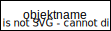
\includegraphics{Bilder/Kapitel-4/objekt_in_uml-darstellung.pdf}
	\caption{Ein Objekt in UML-Darstellung}
	\label{fig:objekt_in_uml-darstellung}
\end{figure}

Nach UML-Konvention wird der Objektname unterstrichen dargestellt. Üblich – obwohl die UML diesbezüglich keine Vorgaben macht – ist außerdem, dass Objektnamen mit einem Kleinbuchstaben beginnen und zentriert dargestellt werden. Innerhalb eines Diagramms müssen die Objektnamen eindeutig gewählt werden. Sollten innerhalb eines Diagramms trotzdem zwei Kästchen denselben Namen enthalten – die UML verbietet dies nicht –, so ist mit beiden Kästchen dasselbe Objekt gemeint. Die doppelte Darstellung eines Objekts wird vor allem in handschriftlich erstellten oder sehr umfangreichen Objektdiagrammen aus Lesbarkeitsgründen verwendet.

\vspace{2mm} %%% für Druck

\begin{figure}[h!]
	\centering
	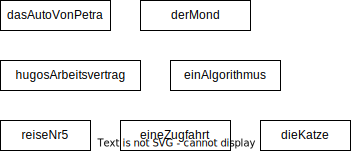
\includegraphics{Bilder/Kapitel-4/objektdiagramm_unverbundene_objekte.pdf}
	\caption{Ein Objektdiagramm mit sieben unverbundenen Objekten}
	\label{fig:objektdiagramm_unverbundene_objekte}
\end{figure}

Abbildung~\ref{fig:objektdiagramm_unverbundene_objekte} zeigt weitere Objekte in UML-Darstellung. Bei manchen wird aus dem Namen (relativ) deutlich, welches konkrete Realwelt-Objekt gemeint ist. So ist \linebreak \sttpUMLText{dasAutoVonPetra}, sofern man Petra kennt und sie nicht mehr als ein Auto besitzt, einem konkreten Realwelt-Auto zuordenbar. Für \sttpUMLText{reiseNr5} bedarf es dagegen schon der zusätzlichen Kenntnis des Kontexts (\zb die Auflistung von Reisen in einem Katalog), um eine Realwelt-Reise mit diesem Namen zu verbinden. Für Objekte wie \sttpUMLText{einAlgorithmus} oder \sttpUMLText{eineZugfahrt} und auch \sttpUMLText{dieKatze} lassen sich die gemeinten Realweltentsprechungen nicht bestimmen. 

Zumindest könnte man aber anhand der Namen der Objekte vielleicht auf die \textbf{Art} des Realwelt-Objekts schließen? So sollte es sich bei \sttpUMLText{dieKatze} doch wohl um eine Katze und nicht um einen Hund handeln? Doch vielleicht trägt mein Realwelt-Meerschweinchen – aus welchem Grund auch immer – den Namen \sttpUMLText{dieKatze} und meine Realwelt-Katze heißt stattdessen \sttpUMLText{pünktchen}. Der modellierten Abstraktion des Realwelt-Objekts kann man den Typ des Objekts in der bisher gewählten Darstellungsform also nicht ansehen. 

Um den Typ eines modellierten Realwelt-Objekts anzugeben, wird in der UML-Dar\-stel\-lung des Objekts der Objektname um die Angabe des Namens der \textit{Klasse}
\marginline{Klasse}
ergänzt (Abb.~\ref{fig:darstellung_objekt} rechts). Die Objektdarstellung ohne zusätzlichen Klassennamen (wie in Abb.~\ref{fig:darstellung_objekt} links und den vorherigen Abbildungen) ist nach UML-Regeln zulässig, sollte aus semantischen Gründen aber nur dann verwendet werden, wenn der Zielgruppe des Modells der Typ des Objekts bekannt ist.

\begin{figure}[h!]
	\centering
	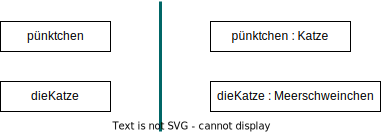
\includegraphics{Bilder/Kapitel-4/darstellung_objekt.pdf}
	\caption[Ein Katzen-Objekt namens \sttpUMLText{pünktchen} und ein Meerschweinchen-Objekt namens \sttpUMLText{dieKatze}]{Ein Objekt namens \sttpUMLText{pünktchen} und ein Objekt namens \sttpUMLText{dieKatze} (links). Ein Katzen-Objekt namens \sttpUMLText{pünktchen} und ein Meerschweinchen-Objekt namens \sttpUMLText{dieKatze} (rechts). Der senkrechte Strich in der Abbildung trennt die linke und die rechte Seite dieser Abbildung. Er ist nicht Bestandteil eines UML-Objektdiagramms.}
	\label{fig:darstellung_objekt}
\end{figure}


\sttpHinweiskasten{1.0}{CamelCase-Schreibweise}{Bezeichner (Namen) in Programmcode dürfen häufig keine Leerzeichen enthalten. Die sogenannte CamelCase-Schreibweise, bei der das erste Wort kleingeschrieben wird und alle folgenden jeweils mit einem Großbuchstaben beginnen, ist eine Möglichkeit, auch ohne Trennzeichen ausdrucksstärkere Bezeichner als \zb \sttpUMLText{auto1} und \sttpUMLText{auto2} zu verwenden. Die CamelCase-Schreibweise findet man auch in Domänenmodellen häufig, obwohl Domänenmodelle eigentlich noch von Implementierungsaspekten abstrahieren sollten und hier die Verwendung von Leerzeichen Realwelt-näher wäre. Die UML selber macht keine Vorgaben oder Einschränkungen bezüglich der Schreibweise der Namen, spezifische UML-Werkzeuge tun dies allerdings teilweise schon.}

Abbildung~\ref{fig:sechs_mal_katze} zeigt weitere Katzen-Objekte. Wichtig ist, dass jeweils ausschließlich die Angabe \sttpUMLText{:Katze} bestimmt, dass es sich um ein Objekt vom Typ Katze handelt. Die beiden unteren Objekte in der Abbildung sind sogenannte \textit{anonyme Objekte}.
\marginline{anonymes Objekt}
Diese Form der Darstellung wird verwendet, wenn man nicht ein konkretes, mit einem Namen versehenes, Katzen-Objekt modellieren möchte, sondern \textbf{irgendein} Objekt vom Typ Katze. Beachten Sie, dass auch ein anonymes Objekt nur genau \textbf{ein} Objekt ist. Es steht nicht stellvertretend für beliebig viele Katzen-Objekte. Im Unterschied zu benannten Objekten handelt es sich bei mehreren anonymen Objekten derselben Klasse im selben Objektdiagramm nach UML-Definition um \textbf{unterschiedliche} Objekte. Die beiden anonymen Katzen-Objekte in Abbildung~\ref{fig:sechs_mal_katze} modellieren daher zwei unterschiedliche Realwelt-Katzen, bei denen es aber für den Modellierungszweck irrelevant ist, um welche konkreten Realwelt-Katzen es sich handelt. Das Objekt mit Namen \sttpUMLText{eineKatze} ist dagegen kein anonymes Objekt, sondern modelliert genau diejenige Realwelt-Katze, die den Namen \sttpUMLText{eineKatze} trägt.

\begin{figure}[h!]
	\centering
	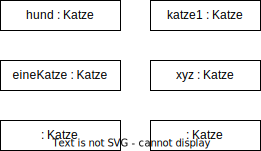
\includegraphics{Bilder/Kapitel-4/sechs_mal_katze.pdf}
	\caption{Vier benannte und zwei anonyme Objekte der Klasse \sttpUMLText{Katze}}
	\label{fig:sechs_mal_katze}
\end{figure}

Das Konzept der Klasse ist ein zentraler Bestandteil der objektorientierten Softwareentwicklung – auch wenn es einige wenige objektorientierte Programmiersprachen gibt (\zb JavaScript), die keine Klassen, sondern ausschließlich Objekte kennen. Sie kennen aus der objektorientierten Programmierung sicher die Definition einer Klasse als Bauplan bzw. Schablone für gleichartige Software-Objekte. Dabei wird die Klasse aus dem Blickwinkel der Programmcodeerstellung betrachtet. Aber was ist eigentlich eine Klasse, wenn wir mit dem Fokus der Realweltmodellierung hinsehen?

Abbildung~\ref{fig:klassenbegriff} greift das Beispiel mit Herrn Müller aus Abschnitt 3.2.1 (S.~\pageref{fig:mueller_lehrer_fussballer}) wieder auf. Aus dem Realwelt-Objekt Herr Müller wird durch entsprechende (unter\-schied\-liche) Abstraktion das modellierte Realwelt-Objekt Lehrer Müller oder das modellierte Realwelt-Objekt Fußballer Müller. Eine Klasse
\marginline{eine Klasse\\ ist die Beschrei\-bung einer Abstrak\-tion}
beschreibt genau diese Abstraktion zwischen dem Realwelt-Objekt und der Modellierung des Realwelt-Objekts. Die Klasse Lehrer definiert, welche Merkmale des Realwelt-Objekts für die Modellierung als Lehrer Müller relevant sind. Die Klasse Fußballer beschreibt die\-jenigen Merkmale des Realwelt-Objekts, die für die Modellierung als Fußballer Müller relevant sind.

\begin{figure}[h!]
	\centering
	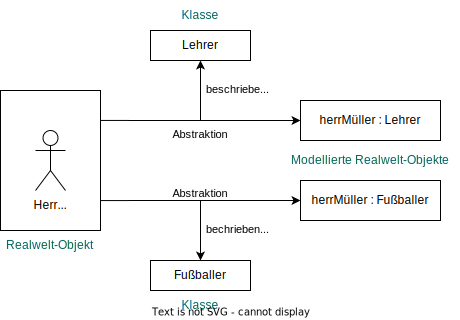
\includegraphics{Bilder/Kapitel-4/klassenbegriff_realweltmodellierung.pdf}
	\caption{Der Klassenbegriff aus Sicht der Realweltmodellierung}
	\label{fig:klassenbegriff}
\end{figure}


Zwei Aspekte zum Konzept der Klasse müssen wir an dieser Stelle noch ergänzen. Erstens gilt die in den Klassen Lehrer und Fußballer beschriebene Abstraktion natürlich nicht nur für das konkrete Realwelt-Objekt Herrn Müller, sondern für alle Realwelt-Objekte (Frau Schulze, Herr Özdemir, Frau Kinsombi,~\ldots), die modellierte Realwelt-Lehrer oder Realwelt-Fußballer werden sollen. Und zweitens beschreibt eine Klasse die Abstraktion zwischen Realwelt-Objekt und Modellierung eines solchen Realwelt-Objekts auch dann, wenn man (noch) gar kein modelliertes Objekt hat. So kann zum Beispiel eine Klasse Katze existieren, die definiert, wie man von einer Realwelt-Katze zu einer modellierten Realwelt-Katze kommen würde, ohne dass es ein modelliertes Katzen-Objekt gibt. Eine Klasse ist somit unabhängig von der Existenz der modellierten Objekte – umgekehrt gilt dies jedoch nicht.

\vspace{\baselineskip} %%% für Druck

\begin{figure}[h!]
	\centering
	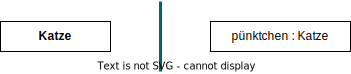
\includegraphics{Bilder/Kapitel-4/darstellung_klasse.pdf}
	\caption[Eine Klasse mit Namen \sttpUMLText{Katze} und ein Objekt dieser Klasse]{Eine Klasse mit Namen \sttpUMLText{Katze} (links) und ein Objekt dieser Klasse mit Namen \sttpUMLText{pünktchen} (rechts)}
	\label{fig:darstellung_klasse}
\end{figure}

\vspace{\baselineskip} %%% für Druck

Die UML-Darstellung einer Klasse ist sehr ähnlich zu der Darstellung eines Objekts. Es handelt sich ebenfalls um ein Rechteck, in dem (mindestens) der Klassenname eingetragen ist. Abbildung~\ref{fig:darstellung_klasse} zeigt links eine Klasse \sttpUMLText{Katze} und rechts ein modelliertes Katzen-Objekt namens \sttpUMLText{pünktchen}. Im Unterschied zu Objekten wird bei der Darstellung einer Klasse der Name nicht unterstrichen. Zudem ist es üblich, den Klassennamen mit einem Großbuchstaben zu beginnen und ihn zentriert und fett gedruckt zu setzen. Der Klassenname ist üblicherweise ein Substantiv im Singular und nicht im Plural. Wie auch bei den benannten Objekten gilt für Klassen in einem Diagramm, dass es sich bei der mehrfachen Darstellung einer Klasse per Defi\-ni\-tion um dieselbe Klasse handelt. Die mehrfache Darstellung von Klassen in einem Diagramm sollte man nur sehr dosiert anwenden, da die existierenden Beziehungen zwischen Klassen (s. Kap. \ref{sec:Kap-4.3}) mit jeder Dopplung einer Klasse im Diagramm weniger gut zu überblicken sind.

Wenn man Softwareprodukte, wie zum Beispiel die erwähnte Schulverwaltungssoftware entwickeln möchte, sind die konkreten Objekte der Realwelt wie Herr Müller meistens weniger interessant. Entscheidender ist, dass die Software später mit beliebigen Objekten eines bestimmten Typs (\zb Lehrer-Objekt) umgehen kann. Die Informationen zu den Merkmalen von Objekttypen finden sich in der objektorientierten Softwareentwicklung aber in den Klassen und nicht in den Objekten. Daher interessieren für die Softwareentwicklung vor allem die Klassen.

Für die Modellierung von Klassen stellt die UML ein eigenes Diagramm, das \textit{Klassen\-diagramm},
\marginline{Einsatzgebiete von Klassen- und Objekt\-diagrammen}
zur Verfügung.  Es gehört wie das Objektdiagramm zu den Struktur\-diagrammen der UML und stellt Klassen und ihre Beziehungen zueinander dar. Das Klassendiagramm ist für das Softwareengineering eine der wichtigsten Diagramm\-arten der UML, da es in fast allen Prozessen des Softwareengineering eingesetzt werden kann. Objektdiagramme dagegen werden in der Praxis seltener eingesetzt. Man kann sie verwenden, um bestimmte Situationen zur Laufzeit des Software\-produkts zu veranschaulichen: Welche Software-Objekte existieren zu einem bestimmten Zeitpunkt und wie stehen sie miteinander in Verbindung. Für die Lehre eignen sich Objekt\-diagramme zudem ganz gut, da sie für Anfänger im Bereich der Objektorientierung die Kluft zwischen den Objekten der Realwelt und den Klassen der objektorientierten Programmierung überbrücken helfen.

\clearpage
\section{Merkmale modellieren}
\label{sec:Kap-4.2}

Merkmale von Realwelt-Objekten, zum Beispiel die Fellfarbe bei Katzen, definiert man in der objektorientierten Softwareentwicklung in den Klassen. Dafür verfügen die Klassen über sogenannte \textit{Attribute}.
\marginline{Attribute}

\vspace{2mm} %%% für Druck

\begin{figure}[h!]
	\centering
	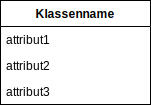
\includegraphics{Bilder/Kapitel-4/darstellung_klasse_mit_drei_attributen.pdf}
	\caption[Die UML-Darstellung einer Klasse]{Die UML-Darstellung einer Klasse mit Angabe des Namens der \mbox{Klasse} und drei Attributen}
	\label{fig:darstellung_klasse_mit_drei_attributen}
\end{figure}

In der UML-Darstellung wird das Rechteck der Klasse durch eine Linie horizontal unterteilt. Oberhalb der Linie steht der schon bekannte Name der Klasse, unterhalb der Linie werden die Attribute, untereinander und linksbündig gesetzt, aufgeführt. Jedes (spätere) Objekt, das nach den Vorgaben der Klasse modelliert wird – man sagt verkürzend: „Jedes Objekt der Klasse“ – verfügt über genau die Attribute, die die Klasse definiert. Die Werte der Attribute, also die Ausprägung der Merkmale, sind dabei jedoch spezifisch pro Objekt.

Wir wechseln von Katzen zu Autos! Abbildung~\ref{fig:klasse_auto_mit_zwei_attributen} zeigt eine Klasse \sttpUMLText{Auto} mit den zwei Attributen \sttpUMLText{modell} und \sttpUMLText{farbe}.

\begin{figure}[h!]
	\centering
	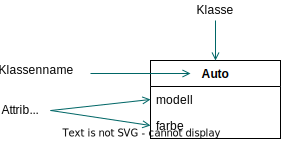
\includegraphics{Bilder/Kapitel-4/klasse_auto_mit_zwei_attributen.pdf}
	\caption{Eine Klasse \sttpUMLText{Auto} mit zwei Attributen}
	\label{fig:klasse_auto_mit_zwei_attributen}
\end{figure}

Abbildung~\ref{fig:drei_mal_klasse_auto_plus_klasse_hugoauto} oben zeigt mit \sttpUMLText{ellensAuto}, \sttpUMLText{heikesAuto} und \sttpUMLText{marvinsAuto} drei Objekte, die die von der Klasse \sttpUMLText{Auto} definierten Merkmale (Vorhandensein der Eigenschaften Modell und Farbe) erfüllen und damit Objekte der Klasse \sttpUMLText{Auto} sind. Die von der Klasse vorgegebenen Attribute sind bei den Objekten mit konkreten Werten belegt: Für das Attribut \sttpUMLText{modell} finden wir hier die Werte Toyota Yaris und VW Golf, für das Attribut \sttpUMLText{farbe} die Werte stahlblau, weiß und rot. Wie hier bei dem \sttpUMLText{modell}-Attribut von \sttpUMLText{ellensAuto} und \sttpUMLText{heikesAuto} können die Werte -- man sagt auch synonym: Wertebelegungen
\marginline{Werte\-belegungen}
-- von Attributen bei unterschiedlichen Objekten auch übereinstimmen. Wenn zwei Objekte derselben Klasse in \textbf{allen} \mbox{Wertebelegungen} der Attribute übereinstimmen, also zum Beispiel Heikes Toyota Yaris auch stahlblau wäre wie der von Ellen, nennt man dies in der Objektorientierung zustandsgleiche Objekte.

\begin{figure}[h!]
	\centering
	\includegraphics{Bilder/Kapitel-4/klasse_auto.pdf}
	\caption[Drei Objekte der Klasse \sttpUMLText{Auto}]{Drei Objekte der Klasse \sttpUMLText{Auto} (oben) und ein Objekt mit Namen \sttpUMLText{hugosAuto}, das kein Objekt der Klasse Auto aus Abbildung~\ref{fig:klasse_auto_mit_zwei_attributen} ist (unten)}
	\label{fig:drei_mal_klasse_auto_plus_klasse_hugoauto}
\end{figure}

Abbildung~\ref{fig:drei_mal_klasse_auto_plus_klasse_hugoauto} unten
\marginline{der Unterschied zwischen Realwelt-Objekten und modellierten Objekten}
zeigt ein Objekt mit Namen \sttpUMLText{hugosAuto}, das im Gegensatz zu den drei anderen Objekten kein Objekt der in Abbildung~\ref{fig:klasse_auto_mit_zwei_attributen} modellierten Klasse \sttpUMLText{Auto} ist, da es über ein Attribut \sttpUMLText{baujahr} verfügt, das die in Abbildung~\ref{fig:klasse_auto_mit_zwei_attributen} dargestellte Auto-Klasse nicht kennt. An dieser Stelle müssen Sie sich noch einmal den Unterschied zwischen Realwelt-Objekten und den für Softwareengineering-Zwecke modellierten Objekten vergegenwärtigen: Das Realwelt-Auto von Hugo ist sicher genau wie die Autos von Ellen, Heike und Marvin ein Auto. Und die Realwelt-Autos der drei letzteren Personen haben auch genau wie Hugos Auto ein Baujahr. Die in Abbildung~\ref{fig:klasse_auto_mit_zwei_attributen} für einen (hier unbekannten) Zweck im Rahmen des Softwareengineering modellierte Klasse Auto abstrahiert von allen Eigenschaften von Realwelt-Autos, die für den Modellierungszweck nicht relevant sind. Und in diesem Beispiel betrifft das eben auch das Merkmal Baujahr. \textbf{Modellierte} Objekte vom Typ Auto besitzen hier daher kein Attribut \sttpUMLText{baujahr}, auch wenn für ihre Realweltentsprechungen ein Baujahr existiert.

An dem Auto-Baujahr-Beispiel zeigt sich ein weiterer praktischer Verwendungszweck von Objektdiagrammen. In  Diskussionen über die relevanten Strukturen der Domäne zwischen Softwareentwicklungsteam und Kunden kann es für die Kunden schwierig sein, die ihnen bekannte Ebene der Realwelt-Objekte mit der Ebene der deutlich abstrakteren Klassen zusammenzubringen. Hier kann es helfen, statt Klassen zunächst konkrete (Beispiel)Objekte und ihre Eigenschaften zu modellieren und erst anschließend auf dieser Grundlage die benötigten Klassen zu entwerfen.

\clearpage
\section{Beziehungen modellieren}
\label{sec:Kap-4.3}

Um in UML-Objektdiagrammen eine Beziehung zwischen Objekten zu modellieren, verbindet man die Kästen der Objekte mit einer durchgezogenen Linie. Die UML-Termi\-no\-logie für eine Beziehung von Objekten ist \textit{Verbindung} (engl. link). \marginline{Objekt\-verbindungen} Abbildung~\ref{fig:objektdiagramm} zeigt ein Objektdiagramm, das zwei Lehrer-Objekte, drei Fach-Objekte und drei Schüler-Objekte enthält. Zwischen einigen der Objekte bestehen Verbindungen. So hat zum Beispiel das Lehrer-Objekt mit Namen \sttpUMLText{weber} oben links eine Verbindung zum Fach-Objekt \sttpUMLText{sport} und eine weitere zum Fach-Objekt \sttpUMLText{biologie}. Anhand des Namens der Verbindung (\sttpUMLText{unterrichtet}) erkennt man, welche Art von Realweltbeziehung hier abgebildet wird: Der Realwelt-Lehrer Weber unterrichtet die Fächer Sport und Biologie. 

\vspace{\baselineskip} %%% für Druck

\begin{figure}[h!]
	\centering
	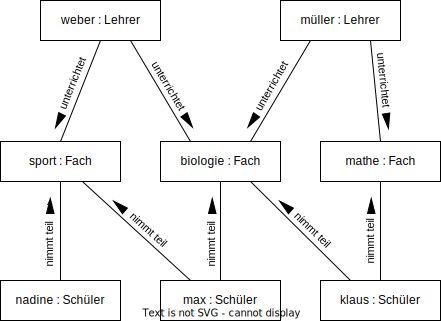
\includegraphics{Bilder/Kapitel-4/objektdiagramm_lehrer_fach_schueler.pdf}
	\caption{Ein Objektdiagramm}
	\label{fig:objektdiagramm}
\end{figure}

\vspace{\baselineskip} %%% für Druck

Das kleine schwarze Dreieck in der Nähe des Verbindungsnamens wird in der UML verwendet, um eine Leserichtung der Verbindung anzugeben. An diesem erkennt man, dass der Lehrer Weber das Fach Sport unterrichtet und nicht das Fach Sport den Lehrer Weber. Wir hätten ebenso gut \sttpUMLText{wird unterrichtet von} als Verbindungsnamen verwenden und das kleine Dreieck entsprechend um 180$^{\circ}$ drehen können. In beiden Fällen ist die Bedeutung der modellierten Beziehung zwischen \sttpUMLText{weber} und \sttpUMLText{sport} identisch. Die Angabe einer Leserichtung ist optional. Man sollte sie explizit angeben, wenn sie sich aus dem Kontext nicht erschließen lässt. Die Angabe eines Verbindungsnamens, der üblicherweise ein Verb enthält, ist im Übrigen auch optional, aber gerade in Domänenmodellen meist hilfreich, um Missverständnisse zwischen Fachanwendern und Softwareentwicklern über den zu modellierenden Real\-welt\-ausschnitt zu vermeiden.

In Abbildung~\ref{fig:objektdiagramm} haben wir auf die Angabe von Attributen der Objekte verzichtet. So werden wir auch in den folgenden Abbildungen verfahren und Attribute immer dann weglassen, wenn sie für die aktuellen Modellierungszwecke (\zb hier: Erläuterung von Objekt- und Klassenbeziehungen) nicht relevant sind. Ein solches Vorgehen ist üblich in der objektorientierten Modellierung. Die UML bietet für ein spezifisches Diagramm (\zb Objektdiagramm) bestimmte Notationselemente an. Bei der Erstellung eines Diagramms müssen aber nicht alle zur Verfügung stehenden Elemente auch eingesetzt werden. Die Auswahl trifft der Modellersteller in Abhängigkeit von Einsatzzweck und Zielgruppe des Modells.

\vspace{2mm} %%% für Druck

\minisec{Klassenbeziehungen spezifizieren Objektbeziehungen}
\phantomsection
\label{sec:Kap-3.2.5.3:klassenbeziehungen}

Ein Objektdiagramm wie in Abbildung~\ref{fig:objektdiagramm} könnte im Rahmen eines Projekts zur Entwicklung einer Schulverwaltungssoftware bei einer Diskussion zwischen dem Softwareentwicklungsteam und den Domänenexperten über die Domäne Schule entstanden sein. Wir wiederholen an dieser Stelle, dass im Softwareengineering die Modellierung der Realwelt kein Selbstzweck ist. Die Realweltmodellierung ist ein (notwendiger) Baustein für das übergeordnete Ziel der Entwicklung (bzw. Weiterentwicklung, Änderung etc.) eines Softwareprodukts. Wie weiter oben erwähnt, benötigt man dafür aber die Klassen und nicht die Objekte. Man muss daher von einem Objektdiagramm wie in Abbildung~\ref{fig:objektdiagramm} zu einem abstrakteren Klassendiagramm kommen. Abbildung~\ref{fig:klassendiagramm_zu_objektdiagramm} zeigt ein solches Klassendiagramm. 

\vspace{\baselineskip} %%% für Druck
\vspace{\baselineskip} %%% für Druck

\begin{figure}[h!]
	\centering
	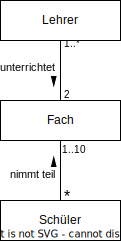
\includegraphics{Bilder/Kapitel-4/klassendiagramm_lehrer_fach_schueler.pdf}
	\caption[Ein zum Objektdiagramm aus Abb.~\ref{fig:objektdiagramm} gehöriges Klassen\-diagramm]{Ein zum Objektdiagramm aus Abbildung~\ref{fig:objektdiagramm} gehöriges Klassen\-diagramm}
	\label{fig:klassendiagramm_zu_objektdiagramm}
\end{figure}

\vspace{\baselineskip} %%% für Druck

Das Klassendiagramm spezifiziert, welche Objekte mit welchen anderen Objekten in welchen Arten von Beziehungen stehen dürfen. Es gibt somit die Regeln vor, anhand derer bestimmt werden kann, ob \marginline{Objekt\-konstellationen}
\textit{Objektkonstellationen} (Menge von Objekten mit oder ohne Verbindungen untereinander) gültig oder ungültig sind. Eine Objektkonstellation ist dann gültig, wenn sie alle durch das Klassendiagramm festgelegten Bedingungen erfüllt, andernfalls ist sie ungültig. Wenn mit einer Objekt\-konstel\-la\-tion wie in Abbildung~\ref{fig:objektdiagramm} begonnen wird, von der die Domänenexperten gesagt haben, dass diese eine adäquate Modellierung der Realweltzusammenhänge darstellt, und sie damit gültig sein soll, muss man das Klassendiagramm und seine Regeln ent\-sprechend so konstruieren, dass alle gültigen Objektkonstellationen der Spezi\-fi\-kation entsprechen. In der Praxis findet häufig aber auch der umgekehrte Weg statt: Man beginnt mit einem Klassendiagramm und erstellt auf dieser Grundlage – im Prinzip nur zu Diskussions- oder Prüfzwecken mit den Domänenexperten – gültige und ungültige Objektkonstellationen.

\vspace{1.4mm} %%% für Druck

Das Klassendiagramm in Abbildung~\ref{fig:klassendiagramm_zu_objektdiagramm} beinhaltet die drei Klassen \sttpUMLText{Lehrer}, \sttpUMLText{Fach} und \sttpUMLText{Schüler}, da für das Objektdiagramm aus Abbildung~\ref{fig:objektdiagramm} Lehrer-Objekte, Fach-Objekte und Schüler-Objekte benötigt werden. Wie zwischen Objekten werden Beziehungen zwischen Klassen in UML durch eine durchgezogene Linie zwischen den Klassen dargestellt. Eine solche Beziehung zwischen Klassen nennt man eine \textit{\mbox{Assoziation}}
\marginline{Assoziationen}
(engl. association). 

\vspace{1.4mm} %%% für Druck

Die Angaben mit Zahlen und Sternchen (*) an den Assoziationsenden in Abbildung~\ref{fig:klassendiagramm_zu_objektdiagramm} heißen \textit{Multiplizitäten}.
\marginline{Multiplizitäten}
Die Multiplizitäten geben an, mit wie vielen anderen Objekten (in Bezug auf die betrachtete Assoziation) die Objekte einer Klasse in Beziehungen stehen können bzw. müssen. Multiplizitäten werden in der Form \sttpUMLText{untereGrenze..obereGrenze} angegeben (\zb \sttpUMLText{1..10}), wobei die untere Grenze die minimale Anzahl und die obere Grenze die maximale Anzahl angibt. Sind untere und obere Grenze identisch, genügt die Angabe eines Werts (\zb \sttpUMLText{2} als Abkürzung für \sttpUMLText{2..2}). Neben der Angabe natürlicher Zahlen kennt die UML in Multiplizitäten noch die Angaben \sttpUMLText{0} und \sttpUMLText{*}. Die \sttpUMLText{0} kann nur als untere Grenze verwendet werden (\zb \sttpUMLText{0..6}) und bedeutet, dass kein verbundenes Objekt gefordert wird. Das Sternchen-Symbol (\sttpUMLText{*}) kann als obere Grenze verwendet werden (wie bei \sttpUMLText{1..*} an der Assoziation \sttpUMLText{unterrichtet}) oder alleine stehen (wie auf der Seite von Schüler an der Assoziation \sttpUMLText{nimmt teil}). Letztere Form ist eine Abkürzung für \sttpUMLText{0..*}, insofern bildet das \sttpUMLText{*} auch hier die obere Grenze. Es bedeutet unbegrenzt viele, wobei unbegrenzt nur nach oben gilt, die angegebene untere Grenze wird durch das Sternchen nicht beeinflusst. Zum Beispiel wären vier Objekte durch die Angabe \sttpUMLText{5..*} nicht abgedeckt, 37~allerdings schon und genauso auch zwei Millionen. 

\vspace{1.4mm} %%% für Druck

Das Lesen
\marginline{Bedeutung von Multiplizitäten}
und das sprachlich adäquate Erläutern der Bedeutung von Multiplizitäten in Klassendiagrammen ist nicht ganz einfach. Ein entscheidender Aspekt, mit dem UML-Anfänger oft Schwierigkeiten haben: Das Klassendiagramm zeigt Klassen und ihre mit Multiplizitäten versehenen Beziehungen zueinander. Die durch die Multiplizitäten modellierten Bedingungen beziehen sich aber nicht auf die Klassen, sondern auf die Objekte dieser Klassen. Man modelliert also Klassen-Beziehungen obwohl man Objekt-Beziehungen spezifizieren möchte.

\vspace{1.4mm} %%% für Druck

Die zweite Schwierigkeit ist, welche Multiplizität die relevante für eine Aussage ist, denn jede Assoziation zwischen zwei Klassen besitzt zwei Multiplizitäten. Wir verlassen kurz Abbildung~\ref{fig:klassendiagramm_zu_objektdiagramm} und wechseln auf ein kleineres Beispiel. Abbildung~\ref{fig:klassendiagramm_und_objektkonstellationen} zeigt oben wieder eine \sttpUMLText{unterrichtet}-Assoziation zwischen einer \sttpUMLText{Lehrer}-Klasse und einer \sttpUMLText{Fach}-Klasse. Die Assoziation weist eine Multiplizität \sttpUMLText{2} auf der Seite der \sttpUMLText{Lehrer}-Klasse und eine Multiplizität \sttpUMLText{3} auf der Seite der \sttpUMLText{Fach}-Klasse auf. 

\pagebreak %%% für Druck

\begin{figure}[h!]
	\vspace{8mm} %%% für Druck
	\centering
	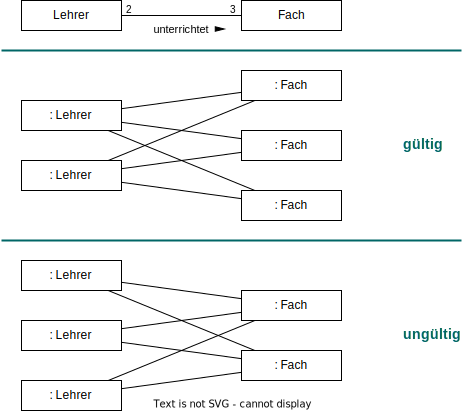
\includegraphics{Bilder/Kapitel-4/objektkonstellation_gueltig_ungueltig.pdf}
	\caption[Klassendiagramm, gültige und ungültige Objektkonstellation]{Ein Klassendiagramm (oben), eine gültige Objektkonstellation (Mitte) und eine ungültige Objektkonstellation (unten)}
	\label{fig:klassendiagramm_und_objektkonstellationen}
\end{figure}

Für Aussagen über die gültigen Verbindungen von Lehrer-Objekten muss (für manchen wenig intuitiv) die Multiplizität auf Seite der \sttpUMLText{Fach}-Klasse betrachtet werden und umgekehrt. Jedes Lehrer-Objekt ist also mit drei Fach-Objekten verbunden und nicht mit zwei und jedes Fach-Objekt mit zwei Lehrer-Objekten und nicht mit drei. Abbildung~\ref{fig:klassendiagramm_und_objektkonstellationen} zeigt in der Mitte eine gültige Objektkonstellation bezüglich des Klassendiagramms und unten eine ungültige Objektkonstellation. Bei Letzterer wurden die Multiplizitäten verkehrt herum gelesen.

Im Prinzip müssten die Assoziationsnamen aus dem Klassendiagramm (in unserem Beispiel \sttpUMLText{unterrichtet}) als Verbindungsnamen in die Objektdiagramme übernommen werden. Aus Übersichtlichkeitsgründen werden in Objektdiagrammen Verbindungsnamen aber häufig nicht angegeben, zumal in der Praxis Objektdiagramme selten ohne Vorliegen bzw. Kenntnis des zugehörigen Klassendiagramms eingesetzt werden, in dem die Assoziationsnamen Auskunft über die Art der Beziehungen zwischen den Objekten geben.

Die dritte Schwierigkeit bei der Interpretation von Multiplizitäten ist zu erkennen, dass mit einer mit Multiplizitäten versehenen Assoziation nicht eine, sondern \textbf{zwei} Aussagen verbunden sind. Die eine Aussage benennt, welche Bedingungen für die Objekte der einen an der Assoziation beteiligten Klasse gelten, die andere gibt an, welche Bedingungen für die Objekte der anderen Klasse gelten. 

\pagebreak %%% für Druck

Wir betrachten weiterhin Abbildung~\ref{fig:klassendiagramm_und_objektkonstellationen}. Es ist nicht möglich, die Bedeutung der beiden Multiplizitäten der Assoziation \sttpUMLText{unterrichtet} in nur einer Formulierung unter\-zubringen. Sätze wie „zwei Lehrer-Objekte stehen in Beziehung mit drei Fach-Objekten“ sind schlichtweg nicht eindeutig. Zwar würden sie durchaus die gültige Objektkonstellation in Abbildung~\ref{fig:klassendiagramm_und_objektkonstellationen} Mitte beschreiben, jedoch auch eine ungültige Objektkonstellation wie in Abbildung~\ref{fig:ungueltige_objektkonstellation} und alle weiteren Beziehungen, in denen zwei Lehrer-Objekte und drei Fach-Objekte vorkommen.

\begin{figure}[h!]
	\centering
	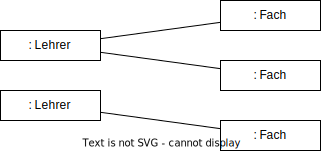
\includegraphics{Bilder/Kapitel-4/ungueltige_objektkonstellation.pdf}
	\caption[Eine ungültige Objektkonstellation zu Abb.~\ref{fig:klassendiagramm_und_objektkonstellationen}]{Eine bezüglich des Klassendiagramms in Abbildung~\ref{fig:klassendiagramm_und_objektkonstellationen} ungültige Objektkonstellation}
	\label{fig:ungueltige_objektkonstellation}
\end{figure}

Es  müssen daher 
\marginline{Multiplizitäten sprachlich ausdrücken}
zwei Aussagen zur Beschreibung der Assoziation verwendet werden: 1. Jedes Lehrer-Objekt ist mit genau drei Fach-Objekten verbunden, 2. Jedes Fach-Objekt (wiederum) ist mit genau zwei Lehrer-Objekten verbunden. Wichtig ist hierbei auch die Formulierung \textbf{jedes} Objekt: Die Vorgaben des Klassendiagramms bezüglich der Verbindungen der Objekte einer Klasse zu anderen Objekten gelten für \textbf{jedes} Objekt dieser Klasse, nicht nur für ein Objekt oder eine bestimmte Teilmenge der Objekte! Wichtig ist auch, dass Multiplizitäten nichts über die \textbf{absolute} Anzahl von Objekten in der Objektkonstellation aussagen.

\sttpHinweiskasten{1.0}{ein vs. jedes}{In der deutschen Sprache verwenden wir in manchen Situationen, in denen wir eigentlich jeder/jede meinen, die Formulierung ein/eine. Zum Beispiel ist mit der Aussage „eine Fichte ist ein Nadelbaum“ vermutlich in den meisten Fällen gemeint, dass es sich bei jeder Fichte um einen Nadelbaum handelt und nicht nur bei einer konkreten Fichte. Eindeutig ist dies aber nicht. Für die sprachliche Erläuterung von Multiplizitäten sollten Sie explizit die Formulierung \textbf{jedes} Objekt verwenden.}

\pagebreak

Kehren wir zum Objektdiagramm aus Abbildung~\ref{fig:objektdiagramm} und zum Klassendiagramm aus Abbildung~\ref{fig:klassendiagramm_zu_objektdiagramm} zurück. 

\begin{center}
	\begin{minipage}[c]{.6\linewidth} 
		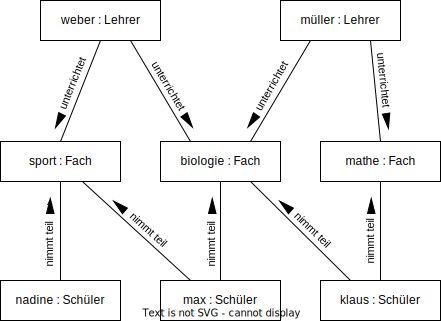
\includegraphics[scale=0.7]{Bilder/Kapitel-4/objektdiagramm_lehrer_fach_schueler.pdf}
	\end{minipage}
	\hspace{.1\linewidth}% Abstand zwischen den beiden Bildern
	\begin{minipage}[c]{.2\linewidth}
		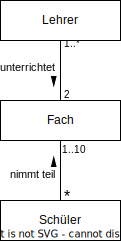
\includegraphics[scale=0.7]{Bilder/Kapitel-4/klassendiagramm_lehrer_fach_schueler.pdf}
	\end{minipage}
\end{center}

Folgende Bedingungen stellt das Klassendiagramm an gültige Objektkonstellationen:
\begin{itemize}
	\item Jedes Lehrer-Objekt ist bezüglich der Verbindungsart \sttpUMLText{unterrichtet} mit genau zwei Fach-Objekten verbunden (Multiplizität: \sttpUMLText{2}). In Realweltterminologie heißt das: Jeder Lehrer unterrichtet genau zwei Fächer.
	\item Jedes Fach-Objekt ist bezüglich der Verbindungsart \sttpUMLText{unterrichtet} mit mindestens einem Lehrer-Objekt verbunden (Multiplizität: \sttpUMLText{1..*}). Realwelt\-termi\-no\-logie: Jedes Fach wird von mindestens einem Lehrer unterrichtet. Auf Grundlage des Objektdiagramms in Abbildung~\ref{fig:objektdiagramm} hätten wir diese Multiplizität durchaus auch weiter einschränken können, denn in Abb.~\ref{fig:objektdiagramm} ist ein konkretes Fach-Objekt entweder mit genau einem Lehrer-Objekt (\sttpUMLText{sport}, \sttpUMLText{mathe}) oder mit genau zwei Lehrer-Objekten (\sttpUMLText{biologie}) verbunden. Die Multiplizität im Klassendiagramm in Abb.~\ref{fig:klassendiagramm_zu_objektdiagramm} hätte also auch \sttpUMLText{1..2} lauten können. Üblicherweise versucht man Multiplizitäten – insbesondere die obere Grenze einer Multiplizität – nicht von Beginn an aufgrund weniger beispielhafter Objekt\-konstellationen zu sehr einzuschränken, da häufig in der weiteren Diskussion mit Domänenexperten doch noch abweichende Fälle auftauchen. Insofern finden sich in den frühen Versionen eines Domänenmodells sehr häufig die Angaben \sttpUMLText{*} oder \sttpUMLText{1..*}. 
	\item Jedes Fach-Objekt ist bezüglich der Verbindungsart \sttpUMLText{nimmt teil} mit beliebig vielen Schüler-Objekten verbunden (Multiplizität \sttpUMLText{*}). Realweltterminologie: An einem (Unterrichts)Fach können beliebig viele (auch keiner!) Schüler teilnehmen. 
	\item Jedes Schüler-Objekt ist bezüglich der Verbindungsart \sttpUMLText{nimmt teil} mit ein bis zehn Fach-Objekten verbunden (Multiplizität: \sttpUMLText{1..10}). Realweltterminologie: Jeder Schüler nimmt mindestens an einem, aber maximal an zehn Fächern teil. 
\end{itemize}

Da wir das Klassendiagramm auf Grundlage der als gültig definierten Objektkonstellation aus Abb.~\ref{fig:objektdiagramm} entsprechend konstruiert haben, erfüllt das Objektdiagramm in Abb.~\ref{fig:objektdiagramm} alle Regeln des Klassendiagramms aus Abb.~\ref{fig:klassendiagramm_zu_objektdiagramm}. Sofern im weiteren Verlauf des Softwareentwicklungsprojekts weitere Objektkonstellationen der Realwelt auftauchen, die ebenfalls gültig sein sollen, muss die aktuelle Version des Klassendiagramms geprüft und unter Umständen angepasst werden.

\minisec{Mehrere Assoziationen zwischen Klassen}

In unserem bisherigen Beispiel waren zwei Objekte immer nur über genau eine Verbindung miteinander verbunden. In der Realwelt existieren aber auch Konstellationen, bei denen zwei Objekte über unterschiedliche Beziehungsarten miteinander verbunden sind. Dies lässt sich auch in der UML modellieren. Abbildung~\ref{fig:assoziationen_zwischen_klassen} zeigt eine Klasse \sttpUMLText{Person} und eine Klasse \sttpUMLText{Glücksspielautomat}. Beide sind durch zwei verschiedene Assoziationen verbunden. Die obere Assoziation bildet ab, dass Personen (in der Realwelt) an Spielautomaten spielen. Die untere Assoziation bildet ab, dass es Personen gibt, die für die Wartung von Spielautomaten zuständig sind. Je nach Art der Beziehung übernehmen Spielautomat-Objekte und Person-Objekte unterschiedliche \marginline{Rollen}
\textit{Rollen}. Achtung: Das ist hier ein anderer Rollenbegriff als der aus Lektion 1.

\vspace{-\baselineskip} %%% für Druck

\begin{figure}[h!]
	\centering
	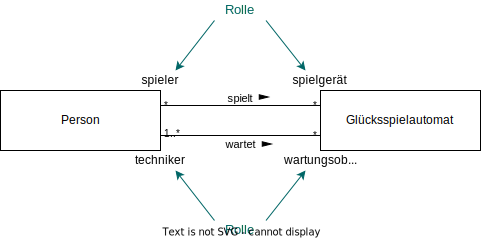
\includegraphics{Bilder/Kapitel-4/assoziationen_zwischen_klassen.pdf}
	\caption{Mehrere Assoziationen zwischen zwei Klassen}
	\label{fig:assoziationen_zwischen_klassen}
\end{figure}

Die  Rollenbezeichnungen können zusätzlich zum Assoziationsnamen an der Assoziation notiert werden, sind aber optional. Rollenbezeichnungen sind im Übrigen nicht auf Situationen beschränkt, in denen mehrere Assoziationen zwischen Klassen modelliert werden sollen. Jede Assoziation kann durch Rollenangaben ergänzt werden. Häufig lassen sich aber schon aus dem Assoziationsnamen die Rollen erschließen, sodass bei nur einer Assoziation zwischen zwei Klassen auf die Angabe von Rollen oft verzichtet wird. Existieren mehrere Assoziationen zwischen Klassen, wie in unserem Spielautomaten-Beispiel, muss aber mindestens eine der beiden Angaben (Assoziationsname oder Rollenbezeichnungen) vorhanden sein, um die Assoziationen unterscheidbar zu halten. 

% Die Grafik ist breiter als die Textbreite.
\begin{figure}[h!]
	\centering
	\includegraphics{Bilder/Kapitel-4/assoziationen_zwischen_klassen_objektdiagramm.pdf}
	\caption[Ein gültiges Objektdiagramm zu Abb.~\ref{fig:assoziationen_zwischen_klassen}]{Ein gültiges Objektdiagramm zu Abbildung~\ref{fig:assoziationen_zwischen_klassen}}
	\label{fig:objektdiagramm_zu_assoziationen_zwischen_klassen}
\end{figure}

Abbildung~\ref{fig:objektdiagramm_zu_assoziationen_zwischen_klassen} zeigt ein Objektdiagramm mit einer gültigen Objektkonstellation bezüglich des Klassendiagramms in Abbildung~\ref{fig:assoziationen_zwischen_klassen}: Sie sehen, dass es Personen geben kann, die an Spielautomaten spielen (Peter), andere die einen Spielautomaten warten (Tom und Mareike), wieder andere, die beides tun (Manfred) und solche, die weder Spieler noch Techniker sind (Hans). All dies lässt das Klassendiagramm aus Abb.~\ref{fig:assoziationen_zwischen_klassen} zu.

\pagebreak %%% für Druck

Abbildung~\ref{fig:tierarzt_tier} zeigt ein weiteres Beispiel für mehrere Assoziationen zwischen Klassen. Zwischen den Klassen \sttpUMLText{Tierarzt} und \sttpUMLText{Tier} gibt es zwei unterschiedliche Beziehungen. Mit der Assoziation \sttpUMLText{impft} soll modelliert werden, dass Tierärzte Tiere impfen. Die Assoziation \sttpUMLText{Jahresuntersuchung} modelliert, dass Tierärzte bei Tieren regelmäßige Vorsorgeuntersuchungen vornehmen. In diesem Beispiel würden sich Rollenbezeichnungen an den beiden Assoziationen nicht sehr voneinander unterscheiden, da das Tier in beiden Fällen eine Art Patient und der Tierarzt eben der Arzt wäre. Man könnte natürlich Rollenbezeichnungen wie \sttpUMLText{impfkandidat}, \sttpUMLText{impfarzt} für die eine Assoziation und \sttpUMLText{patient}, \sttpUMLText{untersuchender} für die andere Assoziation kreieren oder ähnliche voneinander abweichende Formulierungen. Für das Verständnis hilfreicher ist in diesem Beispiel aber der Verzicht auf die Rollenangaben und stattdessen die Verwendung aussagekräftiger Assoziationsnamen. Im Übrigen verwendet man für Assoziationsnamen üblicherweise Verben. Der Assoziationsname \sttpUMLText{Jahresuntersuchung} der unteren Assoziation ist hier aber mal ein Beispiel für einen Fall, in dem ein Nomen als Assoziationsname geeigneter ist als ein Verb.

\begin{figure}[h!]
	\centering
	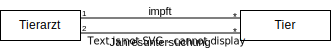
\includegraphics{Bilder/Kapitel-4/tierarzt_tier.pdf}
	\caption[Beispiel für mehrere Assoziationen zwischen Klassen]{Weiteres Beispiel für mehrere Assoziationen zwischen Klassen}
	\label{fig:tierarzt_tier}
\end{figure}

\minisec{Reflexive Assoziationen}

Eine besondere Art von Assoziationen sind sogenannte \textit{reflexive Assoziationen}, die Beziehungen zwischen \textbf{verschiedenen} Objekten \textbf{derselben} Klasse beschreiben. Die Assoziation \sttpUMLText{vertritt} in Abbildung~\ref{fig:assoziation_und_objektkonstellation} oben ist ein Beispiel für eine reflexive Assoziation. Sie beschreibt eine Beziehung zwischen einem Sachbearbeiter-Objekt und anderen Sachbearbeiter-Objekten. Im Beispiel wird modelliert, dass ein Realwelt-Sachbearbeiter durch zwei andere Sachbearbeiter vertreten werden kann (\zb im Urlaubsfall). Abbildung~\ref{fig:assoziation_und_objektkonstellation} unten zeigt eine gültige Objektkonstellation: Der Sachbearbeiter Max steht in seiner Rolle als Verantwortlicher in Verbindungen mit seinen Vertretern den Sachbearbeitern Paul und Hugo. In seiner Rolle als Vertreter steht Max gleichzeitig in Verbindung zur Sachbearbeiterin Sabine, deren Vertretung er übernimmt. In diesem Beispiel ist die Angabe der Rollen für das Verständnis der Beziehungen notwendig. 

\begin{figure}[h!]
	\centering
	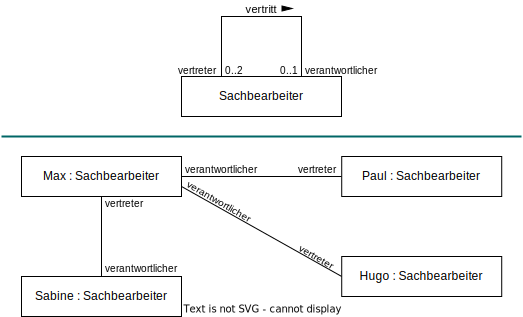
\includegraphics{Bilder/Kapitel-4/sachbearbeiter.pdf}
	\caption[Eine reflexive Assoziation]{Eine reflexive Assoziation (oben) und eine dazu gültige Objekt\-konstellation (unten)}
	\label{fig:assoziation_und_objektkonstellation}
\end{figure}

\minisec{n-äre Beziehungen}
In der Realwelt gibt es Situationen, in denen Objekte von mehr als zwei Klassen miteinander in Beziehung stehen. In der UML drückt man eine solche sogenannte \textit{\mbox{n-äre} Beziehung} zwischen Klassen (\zb drei Klassen: ternär, vier Klassen: quaternär) mit Assoziationen aus, die durch eine Raute verknüpft sind. Abbildung~\ref{fig:tierarzt_tier_krankheit} zeigt ein Beispiel. Zwischen den Klassen \sttpUMLText{Tierarzt}, \sttpUMLText{Tier} und \sttpUMLText{Krankheit} besteht eine Assoziation mit Namen \sttpUMLText{heilt}. Damit soll modelliert werden, dass Tierärzte Tiere von Krankheiten heilen.

\begin{figure}[h!]
	\centering
	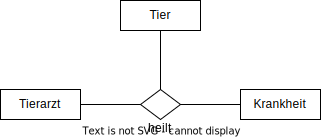
\includegraphics{Bilder/Kapitel-4/tierarzt_tier_krankheit.pdf}
	\caption{Eine Beziehung zwischen drei Klassen}
	\label{fig:tierarzt_tier_krankheit}
\end{figure}

\pagebreak %%% für Druck

Java und viele andere objektorientierte Programmiersprachen unterstützen das Konzept der n-ären Beziehungen nicht, sodass bei der Implementierung solche Assoziationen in mehrere binäre Assoziationen umgewandelt werden müssen. In Domänenmodellen können n-äre Beziehungen aber vorkommen, wenn sie in der Realwelt existieren (und dementsprechend den Domänenexperten geläufig sind), denn Domänenmodelle sollen noch unabhängig sein von jeglichen späteren Implementierungsbedürfnissen.

\minisec{Aggregation und Komposition}
\phantomsection
\label{sec:Kap-3.2.5.3:besondere_assoziationen}

Um weitere besondere Formen von Beziehungen auszudrücken, kennt die UML außer den einfachen Assoziationen, die man mit Assoziationsnamen, Multiplizitäten und Rollen versehen kann, mit der \textit{Aggregation} und der \textit{Komposition} noch zwei spezielle Assoziationen. Mit Aggregation und Komposition lassen sich Teil-Ganzes-Beziehungen modellieren, zum Beispiel ein Einkauf, dessen Teile die einzelnen eingekauften Produkte sind oder ein Haus, das aus mehreren Zimmern besteht. Abbildung~\ref{fig:aggregation_und_komposition} zeigt diese beiden Beispiele. 

\begin{figure}[h!]
	\centering
	\includegraphics{Bilder/Kapitel-4/aggregation_vs_komposition.pdf}
	\caption[Aggregation und Komposition]{Aggregation (links) und Komposition (rechts)}
	\label{fig:aggregation_und_komposition}
\end{figure}

Aggregationsbeziehungen, wie hier zwischen \sttpUMLText{Einkauf} und \sttpUMLText{Produkt}, und Komposi\-tions\-beziehungen, wie zwischen \sttpUMLText{Haus} und \sttpUMLText{Zimmer}, werden durch eine Raute am Assoziationsende des Ganzes-Elements dargestellt. Die unausgefüllte Raute (Abbildung links) kennzeichnet die Aggregation, die ausgefüllte Raute (Abbildung rechts) die Komposition. Assoziationsnamen werden üblicherweise nicht angegeben, da die Art der Beziehung (\sttpUMLText{„besteht aus“}, \sttpUMLText{„hat“}, \sttpUMLText{„setzt sich zusammen aus“},
\sttpUMLText{„ist} \sttpUMLText{Teil} \sttpUMLText{von“} etc.) schon aus der gewählten Verbindungsform hervorgeht.

Aggregation und Komposition drücken im Vergleich zu einfachen Assoziationen eine stärkere Beziehung zwischen den verbundenen Objekten aus, wobei über die Komposition eine noch engere Beziehung modelliert wird als über die Aggrega\-tion. Die Darstellung als Komposition wird verwendet, wenn die Teile (im Beispiel die Zimmer-Objekte) nicht unabhängig vom Ganzen (Haus-Objekt) existieren können, die Verbindung zwischen dem Ganzen und seinen Teilen also untrennbar ist bzw. sein soll. Dementsprechend darf ein konkretes Teil-Objekt auch nur mit einem einzigen Ganzes-Objekt verbunden sein (Multiplizität \sttpUMLText{1} auf der Seite der Klasse \sttpUMLText{Haus}). In Aggregationsbeziehungen ist dagegen die Existenz der Teile (Produkt-Objekte) auch ohne das Ganze (Einkauf-Objekt) vorgesehen.

\minisec{Assoziationsklassen}
Abbildung~\ref{fig:kind_patenschaft_tier} zeigt ein Beispiel für eine sogenannte \textit{Assoziationsklasse}. Mit einer Assoziationsklasse können die Eigenschaften einer Assoziation und die Eigenschaften einer Klasse kombiniert werden. Das macht es möglich, eine Assoziation -- der man nur Namen, Rollen, Multiplizitäten anfügen kann -- zusätzlich mit Merkmalen einer Klasse, wie zum Beispiel Attributen, auszustatten. Man verwendet Assoziations\-klassen, um Charakteristika abzubilden, die Teil der Beziehung zwischen den beteiligten Objekten sind und sich nicht einer der an der Beziehung beteiligten Klassen zuordnen lassen. In unserem Beispiel spielt für eine Patenschaft, die ein Kind für ein Tier übernimmt, der Zeitraum dieser Patenschaft eine Rolle. Diese Information wird als Attribut modelliert.

\begin{figure}[h!]
	\centering
	\includegraphics{Bilder/Kapitel-4/kind_patenschaft_tier.pdf}
	\caption{Eine Assoziationsklasse}
	\label{fig:kind_patenschaft_tier}
\end{figure}

In der UML-Darstellung wird die Assoziationsklasse mit einer gestrichelten Linie an die Assoziationslinie angebunden. Der Name der Assoziationsklasse und der Name der Assoziation müssen identisch sein, wobei letzterer optional ist. Ähnlich wie bei den n-ären Beziehungen müssen Assoziationsklassen-Beziehungen für die Implementierung in andere Beziehungsformen umgewandelt werden, da die objektorientierten Programmiersprachen das Konzept der Assoziationsklasse nicht unterstützen. In \mbox{Domänenmodellen} sind sie aber häufig zu finden.

\minisec{Generalisierung}

Lassen Sie uns zum Schluss des Kapitels noch eine weitere besondere Beziehungsform ansehen, die eine wichtige Rolle in der Objektorientierung spielt. Um (hierarchische) Realweltklassifikationen, sogenannte Taxonomien, abbilden zu können, gibt es das Konzept der \textit{Generalisierung}. Abbildung~\ref{fig:generalisierungsbeziehungen} zeigt die UML-Syntax für die Modellierung von Generalisierungsbeziehungen.

\begin{figure}[h!]
	\centering
	\includegraphics{Bilder/Kapitel-4/generalisierungsbeziehungen.pdf}
	\caption{Generalisierungsbeziehungen}
	\label{fig:generalisierungsbeziehungen}
\end{figure}

Laubbäume und Nadelbäume sind spezielle Formen von Bäumen. In der Terminologie der Objektorientierung sagt man, sie sind \textit{Spezialisierungen} von Bäumen. Die Begriffe Generalisierung und Spezialisierung meinen dasselbe Konzept, sie beschreiben es nur aus zwei unterschiedlichen Richtungen. Ausgehend von der Klasse \sttpUMLText{Baum} sind die Klassen \sttpUMLText{Laubbaum} und \sttpUMLText{Nadelbaum} Spezialisierungen. Aus Richtung der Klasse \sttpUMLText{Laubbaum} bzw. \sttpUMLText{Nadelbaum} betrachtet, ist die Klasse \sttpUMLText{Baum} eine Generalisierung. Die Generalisierungsklasse nennt man auch \textit{Oberklasse},
\marginline{Ober- und Unterklasse}
die Spezialisierungsklasse heißt \textit{Unterklasse}. Generalisierungsbeziehungen sind also Beziehungen zwischen Ober\-klassen und Unterklassen. In der UML wird Generalisierung/Spezialisierung durch einen Pfeil mit einer unausgefüllten Dreiecksspitze auf der Seite der Oberklasse modelliert.

In der Klasse \sttpUMLText{Baum} aus Abb.~\ref{fig:generalisierungsbeziehungen} könnte definiert sein, dass jedes Baum-Objekt eine Wurzel, einen Stamm und Zweige besitzt. Diese Charakteristika der Ober\-klasse gelten in Generalisierungsbeziehungen auch für die Objekte der Unterklassen. In der Terminologie der objektorientierten Programmierung sagt man, die Ober\-klasse \textit{vererbt} Eigenschaften an ihre Unterklasse(n). Die Unterklasse wiederum kann Eigenschaften zu dem Ererbten hinzufügen oder auch Ererbtes verändern, um die Spezialisierung zu charakterisieren. Zum Beispiel charakterisiert einen Laubbaum, dass er Blätter hat, während ein Nadelbaum keine Blätter, sondern Nadeln besitzt. Charakteristisch für eine Birke als Spezialisierung eines Laubbaums ist zum Beispiel die besondere Färbung des Stamms, während eine Eiche, die ebenfalls eine Spezialisierung eines Laubbaums ist, sich durch die Form ihrer Blätter auszeichnet. Auf einer konzeptuellen Ebene ist ein Laubbaum-Objekt aus unserem Beispiel nicht nur ein Laubbaum (hat Blätter) sondern gleichzeitig auch ein Baum (hat Wurzel, Stamm und Zweige). Ein Birke-Objekt ist gleichzeitig eine Birke (Stamm ist weiß), ein Laubbaum (hat Blätter) und ein Baum (hat Wurzel, Stamm und Zweige). 

%--- Kapitel 4.4 KommLit
\clearpage
\section{Kommentierte Literatur}
\label{sec:Kap-4.4}


\sttpKommLitItem{Lahres/Raýman/Strich}{2018}{Objektorientierte Programmierung}{lah18}{Bilder/Buchcover/Buchcover_Lahres_Rayman_Strich.png}{}
{Häufig sind Bücher zu objektorientierter Programmierung eigentlich nur Einführungen in konkrete objektorientierte Programmiersprachen. Das ist hier nicht so. Das Buch beschäftigt sich sehr systematisch und konzeptionell und dabei gut verständlich mit den Prinzipien, der Methodik, den Elementen und dem Einsatz objektorientierter Softwareentwicklung, unabhängig von konkreten Programmiersprachen. Den Schwerpunkt bilden Implementierungsaspekte, dennoch findet man auch viele Informationen zur Objektorientierung im Allgemeinen und Aspekten der objektorientierten Realweltmodellierung. Neben Kapitel~2, das die Objektorientierung im Vergleich zu anderen Programmiermethodiken vorstellt, ist für die Inhalte dieser Lektion vor allem Kapitel~4 relevant. Dieses stellt die Konzepte Objekt und Klasse, ihre Charakteristika und ihre Einsatzmöglichkeiten umfassend vor.}

\sttpKommLitItem{Kecher/Salvanos/Hoffmann-Elbern}{2018}{UML~2.5}{kec18}{Bilder/Buchcover/Buchcover_Kecher_Salvanos.jpg}{}
{Das Kapitel zum UML-Klassendiagramm (S.~37~ff.) ist fast hundert Seiten lang. Sämtliche Elemente, die in einem Klassendiagramm vorkommen können, werden hier gut verständlich mit Realweltbeispielen beschrieben. Bei vielen Elementen wird sogar zusätzlich eine mögliche Umsetzung in Programmcode mit angegeben. Für Anfänger besonders hilfreich sind die Hinweise, für welche Modellierungszwecke sich welche Elemente besonders anbieten.}

\sttpKommLitItem{Sommerville}{2018}{Software Engineering}{som18}{Bilder/Buchcover/Buchcover_Sommerville.jpg}{}
{Kapitel~5 des Lehrbuchs stellt verschiedene Modellarten der UML und ihre Einsatzzwecke im Softwareengineering vor, das UML-Klassendiagramm wird in Kapitel~5.3 behandelt. Im Unterschied zu anderen Lehrbüchern beziehen sich die UML-Beispiele in diesem Buch immer auf eines der vier durchgehenden Fallbeispiele, die in Kapitel~1 vorgestellt werden und sich durch alle Themen des Buchs ziehen. Das hat den Vorteil, dass man sich nicht ständig in neue Kontexte einarbeiten muss, wenn man auch andere Softwareengineering-Themen mit diesem Buch lernen möchte; aber auch den Nachteil, dass es nicht immer die am intuitivsten passenden Beispiele für ein konkretes UML-Konzept sind. Insgesamt ist es gerade für Objektorientierung- und UML-Anfänger sehr zu empfehlen, mit mehreren Büchern zu arbeiten, da jede Autorin/ jeder Autor einen etwas (oder auch sehr) anderen Zugang zum Thema hat.}

\sttpKommLitItem{Brügge/Dutoit}{2006}{Objektorientierte Softwaretechnik}{bru06}{Bilder/Buchcover/Buchcover_Bruegge_Dutoit.jpg}{}
{Kapitel~2.3 des Lehrbuchs stellt unter anderem die Begriffe Modellierung, Objekt, Klasse, Datentyp und Domäne vor. Kapitel~2.4 beschäftigt sich mit unterschiedlichen Diagrammarten der UML, unter anderem mit dem Klassendiagramm. Hier wird auf knapp zehn Seiten ein guter erster Einblick in die wichtigsten Aspekte des UML-Klassendiagramms anhand verschiedener Beispiele gegeben. Für eine intensivere Beschäftigung mit Klassendiagrammen – und anderen UML-Diagrammen – sollte man aber immer auch die speziellen UML-Bücher wie \cite{kec18} zu Rate ziehen.}

\sttpKommLitItem{Oestereich/Scheithauer}{2013}{Analyse und Design mit der UML~2.5}{oes13}{Bilder/Buchcover/Buchcover_Oesterreich_Scheithauer.jpg}{}
{Abschnitt~7 (S.~17~ff) enthält eine Einführung in die Objektorientierung mit den wichtigsten Aspekten in Bezug auf Klassen und Objekte.}



%Zoo
\cleardoublepage
% Kapitel Fallbeispiel Zoo: über das Marko werden Kapitel, Eintrag Inhaltsverzeichnis und die Kopfzeilen konfiguriert.
\FallBeispielZoo
\label{sec:Lektion-2-Zoo}

\marginline{~\\Lektion~1, Seite~\pageref*{sec:Lektion-1-Zoo}}
\sttpUniversalkasten{Was bisher geschah}{Der städtische Zoo ist an das Softwareunternehmen herangetreten, in dem Sie arbeiten, um zu eruieren, an welchen Stellen Zooabläufe mit Software unterstützt werden könnten und wie der öffentliche Zooauftritt insgesamt digitaler werden kann. Welche Dienstleistungen der Zoo von Ihrem Unternehmen erwartet, ist aktuell noch recht vage. \newline \newline	
Wir befinden uns in einer ersten Brainstorming-Besprechung zwischen dem Softwareentwicklungsteam und einer Abordnung des Zoos. Frau Dr. Walther, die Zoodirektorin, hat soeben in einem sehr informationsdichten Rundumschlag zur Domäne Zoo erzählt und dabei auch erste Andeutungen gemacht, für welche Aspekte sie sich Softwareunterstützung vorstellen könnte.}

\minisec{Die Besprechung wird fortgesetzt}

Ihr Chef, Herr Steiber, bedankt sich bei der Zoodirektorin für ihre Ausführungen. Im Anschluss wird frei diskutiert, es wird nachgefragt, zusätzliche Informationen werden erteilt, Unklarheiten angesprochen, manches konkretisiert, anderes im Vagen gelassen, weitere Wünsche geäußert, jede und jeder macht sich ein paar Notizen,~\ldots 
\linebreak
Auf diese Weise sind schnell zwei Stunden vergangen. Die Chemie scheint zu stimmen zwischen dem Zoo- und dem Softwareentwicklungsteam.

Herr Steiber und die Zoodirektorin haben dann auch zwischenzeitlich eine Kaffeepause genutzt, um sich grundsätzlich auf die Zusammenarbeit zu verständigen. Man definiert die heutige Besprechung als Beginn eines kleineren Vorprojekts, in dem der inhaltliche und zeitliche Rahmen für das hoffentlich anschließende eigentliche Softwareentwicklungsprojekt verhandelt wird. Herr Steiber konnte der Zoo\-direk\-torin auch schon mal vorsichtig nahebringen, dass es sicher nicht auf eine allumfassende vollintegrierte und automatisierte Zooverwaltungs- und Zoodigitalisierungssoftware hinauslaufen wird.

\textbf{Hr. Steiber:} „Ich darf um Ihre Aufmerksamkeit bitten! Schön, dass wir schon so intensiv ins Diskutieren gekommen sind. Wir sollten unseren Austausch jetzt aber etwas systematisieren und vor allem unsere Gedanken festhalten. Daher bitte ich Sie, auf den Karteikarten die noch offenen Fragen zur Domäne zu notieren. Erstellen Sie dort bitte auch kurze Beschreibungen der Zoo-Abläufe und -Aufgaben, über die wir hier gerade diskutiert hatten. Einige von Ihnen hatten sich vorhin zudem schon erste Gedanken über das zukünftige Softwareprodukt gemacht, halten Sie das bitte auch alles auf den Karteikarten fest. Und Kollege Fryt, beginnen Sie doch bitte parallel schon mal mit einem ersten groben Domänenklassendiagramm, Sie sehen ja, welche Informationen zur Domäne die anderen ans Whiteboard heften. Aber verlieren Sie sich bloß noch nicht im Detail, da wird es sicher noch viele Änderungen geben, wenn wir uns weiter über die Domäne austauschen.“

\minisec{Einige Zeit später}

% Anmerkung: man kann die Verweise noch wie gewünscht anpassen. Wenn der Verweis hinter den Grafiken stört (roter Rahmen), dann nimmt man "\hyperref[...]{}" weg und lässt nur den 2. Parameter in der geschweiften Klammer stehen. Bei den Bildunterschriften kann man ebenfalls frei entscheiden, wie es aussehen soll.

\begin{center}
	\begin{minipage}[c]{.65\linewidth}
		\centering
		\hyperref[text:lektion2_whiteboard_s1]{\includegraphics[width=0.45\linewidth]{Bilder/Zoo/whiteboard_s1.png} \includegraphics[width=0.45\linewidth]{Bilder/Zoo/whiteboard_s2.png}}
		Whiteboard mit Karteikarten (vergrößerte Darstellung auf Seite~\pageref{text:lektion2_whiteboard_s1}f.)
	\end{minipage}
	\hspace{0.1cm}% Abstand zwischen den beiden Bildern
	\begin{minipage}[c]{.33\linewidth}
		\centering
		\hyperref[fig:lektion2_fallbeispiel_zoo]{\includegraphics[width=\linewidth]{Bilder/Zoo/fallbeispiel_zoo.pdf}}
		Domänenklassendiagramm Zoo (vergrößert in Abbildung~\ref{fig:lektion2_fallbeispiel_zoo})
	\end{minipage}
\end{center}

\textbf{Hr. Steiber:} „Ich danke Ihnen allen! Für das erste Treffen waren wir doch schon sehr produktiv. Sie haben ja schon mitbekommen, dass mit diesem Treffen unser Vorprojekt nun offiziell gestartet ist. Wir werden uns in den nächsten Tagen und Wochen in kleineren Runden wieder treffen und zum einen an der Modellierung der Domäne weiterarbeiten und zum anderen uns natürlich über den Inhalt des zu entwickelnden Softwareprodukts Gedanken machen. Die Kollegin Schwab wird als sehr erfahrene Projektleiterin die Leitung des Vorprojekts übernehmen und zeitnah die verschiedenen Arbeitsgruppen einteilen. Für heute beende ich die Besprechung und wünsche uns allen einen schönen Feierabend.“

\minisec{Am nächsten Tag im Softwareunternehmen}
Die drei Kolleg:innen Inga Schwab (Projektleiterin Vorprojekt), Magnus Fryt (Requirement Engineer) und Joris Jonson (Softwarearchitekt) sitzen zusammen und planen die nächsten Schritte.

\textbf{Inga Schwab:} „Die Domäne Zoo ist komplexer, als ich das gedacht hatte. Unser aktuelles Domänenmodell ist noch viel zu grob. Lasst uns zunächst mal bei der Klasse Tier und der Klasse Tierpfleger ansetzen. Diese Informationen werden wir in jedem Fall brauchen, unabhängig davon, auf welche Aufgabenbereiche für das Softwareprodukt wir uns einigen. Tier scheint nicht gleich Tier zu sein. Ich habe den Eindruck, dass Strukturen und Abläufe der Domäne durchaus unterschiedlich aussehen, je nachdem über welche Tierart wir sprechen. Und auch bei den Tier\-pflegern scheinen Arbeitsabläufe davon abhängig zu sein, welche Tierarten sie betreuen. Was mir gestern, trotz der umfangreichen Erklärungsversuche des Zoo-Teams, bis zum Schluss nicht klar geworden ist, warum es einen auf Löwen spezialisierten Tier\-pfleger geben muss und einen anderen Tierpfleger für die Tiger, die Nagetiere und die Fische aber vom selben Tierpfleger versorgt werden können. Möglicherweise ist das nur historisch so gewachsen im Zoo, aber wir müssen sicher sein, dass uns hier nicht grundlegende Restriktionen der Domäne entgehen. Magnus, übernimm du bitte die Leitung der Arbeitsgruppe Domänenmodellierung. Hol dir Paul dazu, er hat sich in der Besprechung gestern schon gut in die Domäne herein gedacht. Von der Zooseite aus versuche ich dir zwei bis drei der Tierpfleger für die Arbeitsgruppe zu organisieren. Joris, du und ich werden uns mit der Zoo-Führung zusammensetzen und in die Entwicklungsplanung einsteigen, erste Prioritäten hat Frau Dr. Walther ja gestern immerhin schon gesetzt.“

% Das Whiteboard wird auf 2 Seiten dargestellt und soll somit auf einer linken Seite beginnen.
\cleardoubleevenemptypage 

\newgeometry{left=25mm, right=15mm, top=20mm, bottom=20mm,
	marginparwidth=5mm, marginparsep=1mm}
%TODO @Maren: Falls diese Seite wieder eine Kopfzeile haben soll, muss die folgende Zeile - \thispagestyle{empty} - auskommenitert werden.
\thispagestyle{empty}

\phantomsection
\label{text:lektion2_whiteboard_s1}
\minisec{\hspace{1cm}Whiteboard mit Karteikarten}

%\begin{figure}[h!]

{ %% Scope beginnen (damit \renewcommand keine Auswirkung auf andere Karteikarten hat)
	\setlength{\unitlength}{1mm}
	\renewcommand{\sttpKarteikarteSkalierungsfaktor}{0.85}
	
	\begin{picture}(0,0)
		\put(-35,-44){
			\renewcommand{\sttpKarteikarteRotierungswinkel}{0}
			\input{Karteikarten/karteikarte_tierarztFrage.tex}
		}
		\put(48,-45){
			\renewcommand{\sttpKarteikarteRotierungswinkel}{-4}
			\input{Karteikarten/karteikarte_standardSoftware.tex}
		}
		\put(12,-116){
			\renewcommand{\sttpKarteikarteRotierungswinkel}{-2}
			\input{Karteikarten/karteikarte_tierpflegerAufgaben.tex}
		}
		\put(-41,-170){
			\renewcommand{\sttpKarteikarteRotierungswinkel}{2}
			\input{Karteikarten/karteikarte__dummy5.tex}
		}
		\put(42,-177){
			\renewcommand{\sttpKarteikarteRotierungswinkel}{-1}
			\input{Karteikarten/karteikarte_kaefige.tex}
		}
		\put(64,-232){
			\renewcommand{\sttpKarteikarteRotierungswinkel}{-3}
			\input{Karteikarten/karteikarte__dummy3.tex}
		}
		\put(-20,-247){
			\renewcommand{\sttpKarteikarteRotierungswinkel}{1}
			\input{Karteikarten/karteikarte_prioritaeten.tex}
		}
	\end{picture}
} %% Scope beenden (um \renewcommand lokal zu halten)

%\caption{Whiteboard}
%\label{fig:lektion2_whiteboard_s1}
%\end{figure}

\restoregeometry

\clearpage

\newgeometry{left=25mm, right=15mm, top=20mm, bottom=20mm,
	marginparwidth=5mm, marginparsep=1mm}
%TODO @Maren: Falls diese Seite wieder eine Kopfzeile haben soll, muss die folgende Zeile - \thispagestyle{empty} - auskommenitert werden.
\thispagestyle{empty}

\phantomsection
\label{text:lektion2_whiteboard_s2}
% Keine Überschrift hier, aber selben Platz verbrauchen ;-)
\minisec{~~~}

%\begin{figure}[h!]

{ %% Scope beginnen (damit \renewcommand keine Auswirkung auf andere Karteikarten hat)
	\setlength{\unitlength}{1mm}
	\renewcommand{\sttpKarteikarteSkalierungsfaktor}{0.85}
	
	\begin{picture}(0,0)
		\put(-30,-54){
			\renewcommand{\sttpKarteikarteRotierungswinkel}{2}
			\input{Karteikarten/karteikarte_tierarztAufgaben.tex}
		}
		\put(58,-55){
			\renewcommand{\sttpKarteikarteRotierungswinkel}{-2}
			\input{Karteikarten/karteikarte__dummy4.tex}
		}
		\put(32,-123){
			\renewcommand{\sttpKarteikarteRotierungswinkel}{-3}
			\input{Karteikarten/karteikarte_patenschaft.tex}
		}
		\put(10,-180){
			\renewcommand{\sttpKarteikarteRotierungswinkel}{1}
			\input{Karteikarten/karteikarte_gehege.tex}
		}
		\put(-28,-240){
			\renewcommand{\sttpKarteikarteRotierungswinkel}{3}
			\input{Karteikarten/karteikarte_infosTiere.tex}
		}
		\put(-45,-120){
			\renewcommand{\sttpKarteikarteRotierungswinkel}{1}
			\input{Karteikarten/karteikarte__dummy2.tex}
		}
		\put(57,-242){
			\renewcommand{\sttpKarteikarteRotierungswinkel}{-2}
			\input{Karteikarten/karteikarte_tierpflegerFrage.tex}
		}
		%		\put(-20,-247){
			%			\renewcommand{\sttpKarteikarteRotierungswinkel}{1}
			%			\input{Karteikarten/xxx.tex}
			%		}
	\end{picture}
} %% Scope beenden (um \renewcommand lokal zu halten)

%\caption{Whiteboard}
%\label{fig:lektion2_whiteboard_s2}
%\end{figure}

\restoregeometry

\clearpage

\vspace*{4cm} %%% Abbildung auf Seite zentrieren

\begin{figure}[h!]
	\centering
	\includegraphics{Bilder/Zoo/fallbeispiel_zoo.pdf}
	\caption{Domänenklassendiagramm für den Zoo}
	\label{fig:lektion2_fallbeispiel_zoo}
\end{figure}

	
	% Literaturverzeichnis für diese Lektion
	\cleardoublepage % auf einer neuen rechten Seite
	\printbibliography[heading=subbibliography]
\end{refsection}

%--- Lektion 2 --- ENDE
%----------------------------
%--- Lektion 3 --- BEGINN
\cleardoublepage
\part{Prozessmodellierung mit Petrinetzen}
\label{sec:Lektion-3}
% wenn Änderungen zur Vorversion auf der Rückseite des Deckblatts vermerkt werden sollen, hier Auskommentierung rausnehmen
\sttpDeckblattRueckseite{\partname~\thepart}%{\input{Lektion-3/Lektion-3-Text_fuer_Rueckseite.tex}}

\cleardoublepage
\chaptertoc % Inhaltsverzeichnis nur für diese Lektion

\begin{refsection}
	%% Einbinden der einzelnen Kapitel
\cleardoublepage
\chapter*{Vorwort}
\addcontentsline{toc}{chapter}{Vorwort}
\markboth{Vorwort}{Vorwort}

Diese Lektion wurde zum Sommersemester 2024 in Form einer Video-Vorlesungs\-reihe konzipiert, die Sie im Moodleauftritt des Moduls finden. Die Entscheidung für Videos begründete sich auf dem Wunsch vieler Studierender audiovisuelle Lernmaterialien nutzen zu können, vor allem aber in der besseren Darstellbarkeit von Prozessen und ihren Modellen, die im Videoformat Schritt-für-Schritt entwickelt und erklärt werden können. Nutzen Sie die Möglichkeit die Video-Vorlesungen zu verfolgen, um ein umfassendes Verständnis der behandelten Konzepte zu erlangen. Diese textuelle Version enthält zwar auch die meisten Inhalte aus den Vorlesungen, behandelt die Themen allerdings weniger ausführlich.

Hinweis: In diesem Kapitel werden Ihnen an vielen Stellen formale Beweise begegnen. Das Verständnis, aber auch die eigene Formulierung von Beweisen sowie die Anwendung formaler Methoden sind grundlegend für die Entwicklung zuverlässiger und fehlerfreier Software und eine wichtige Kernkompetenz im Softwareengineering. Befassen Sie sich also intensiv damit – nicht nur, weil es erwartet wird, sondern auch, weil es Ihnen letztlich tatsächlich nützen wird. Die Übungs- und Einsendeaufgaben zu dieser Lektion sind ein Anhaltspunkt dafür, wann wir eigene Beweise von Ihnen erwarten und wann das Verstehen der Beweise aus der Vorlesung bzw. aus diesem Text ausreicht.
\cleardoublepage
\chapter*{Einleitung zur Lektion}
\addcontentsline{toc}{chapter}{Einleitung zur Lektion}
\markboth{Einleitung zur Lektion}{Einleitung zur Lektion}

In Lektion 2 haben wir die Grundprinzipien der Modellierung vorgestellt,  
\marginline{Modell und Veränderung}
basierend auf der Definition von Herbert Stachowiak: Modelle sind Abstraktionen natürlicher oder künstlicher Originale, deren Eigenschaften vereinfacht dargestellt oder weggelassen werden, um innerhalb eines Geltungsbereichs für eine bestimmte Zielgruppe spezifische Zwecke zu erfüllen. Auf diesem Verständnis aufbauend haben Sie die Modellierungssprache UML kennengelernt und in Objekt- und Klassendiagrammen strukturelle Aspekte der Realwelt visualisiert. Dabei haben Sie gesehen, dass sich die Objekte der Klassen ändern können: Es können Objekte erzeugt werden, es können sich Attributwerte und damit Objektzustände verändern, Verbindungen können hinzugefügt oder gelöscht werden. Dies geschieht natürlich, weil entsprechende Veränderungen der Realwelt abgebildet werden sollen. Und insbesondere auch, weil dies Auswirkungen der Abläufe sind, die unsere Software realisieren soll.

Klassendiagramme formulieren Regeln, die immer gelten, 
\marginline{Modellierung von Verhalten}
während zugehörige Objektkonstellationen nur für einen bestimmten Zeitpunkt gelten, also Momentaufnahmen eines eventuell komplexen und verteilten Systems darstellen. Die Konstellationen von Objekten können sich auf vielfältige Weise ändern, doch sind diese Änderungen nicht beliebig und nicht unabhängig voneinander, weil ansonsten die genannten Regeln verletzt werden können. Mögliche Änderungen werden durch das Verhalten von Systemen und Prozessen (den Unterschied werden Sie später kennenlernen) beschrieben, und auch dafür braucht es Modelle. Diese Lektion behandelt die Modellierung von Verhalten. Wir werden Modelle zum Verständnis von Verhalten in der Realwelt einsetzen, aber auch zur Beschreibung des Verhaltens von Software.

Prozessmodellierung, 
\marginline{Prozess\-modellierung}
wie sie Ihnen im professionellen Kontext und in der Literatur begegnet, findet Anwendung sowohl in der Informatik als auch in der Wirt\-schafts\-infor\-matik (sie spielt dort insbesondere bei der Optimierung von Geschäftsprozessen eine Rolle). Sie lässt sich also im interdisziplinären Kontext dieser beiden Disziplinen verorten. Seit den späten 1970er Jahren haben sich viele verschiedene Modellierungssprachen für Prozesse entwickelt. Diese Sprachen variieren in ihren spezifischen Ausdrucksformen und Schwerpunkten. In unserer Lehrveranstaltung verwenden wir Petrinetze für die Prozessmodellierung.

\pagebreak %%% für Druck

\sttpAutorenkasten{Carl Adam Petri}{1926}{2010}{Deutscher Mathematiker und Informatiker. Leitete ein Institut der Gesellschaft für Mathematik und Datenverarbeitung (GMD) in St. Augustin bei Bonn. Bekannt ist er vor allem für die nach ihm benannten Petrinetze zur Modellierung des Verhaltens verteilter Systeme.}{Bilder/Autoren/petri.jpg}{2009}{Michael Krapp, \href{http://creativecommons.org/licenses/by-sa/3.0}{CC BY-SA 3.0}, via \href{https://commons.wikimedia.org/wiki/File:Carl_adam_petri.jpg}{Wikimedia Commons}}

\vspace{-1ex} %%% für Druck

\subsection*{Warum Petrinetze?}

\textbf{Petrinetze als Grundlage für andere Prozess-Modellierungssprachen}\\
Obwohl Petrinetze in der praktischen Anwendung möglicherweise nicht (mehr) weit verbreitet sind, bilden sie die theoretische Grundlage für beinahe alle anderen Pro\-zess-Model\-lie\-rungs\-tech\-niken und -sprachen.

\textbf{Einfache Visualisierung}\\
Petrinetze verfügen über eine leicht erlernbare und verständliche grafische Darstellungsform, die nur wenige unterschiedliche Elemente beinhaltet.

\textbf{Modellierung verteilter Systeme mit verteilten, lokalen Zuständen}\\
In verteilten Systemen führen die möglichen Kombinationen der lokalen Zustände der Komponenten zu einer exponentiellen Zunahme möglicher globaler Zustände. Petrinetze bewältigen diese Komplexität, indem globale Zustände nicht explizit modelliert werden, sondern sich aus den Kombinationen der lokalen Zustände ergeben. So wächst die Größe eines Petrinetzes nur linear mit der Systemgröße, was eine effi\-zi\-ente und doch präzise Modellierung großer Systeme ermöglicht. Diese Art der Modellierung hat nicht nur den Vorteil die Komplexität des Modells überschaubar zu halten, sondern spiegelt auch die modulare Struktur des modellierten Systems wider.

\textbf{Präzise Darstellung des Verhaltens von Systemkomponenten}\\
Die Modellierung komplexer Prozesse in der Softwareentwicklung mithilfe von Petrinetzen erlaubt ein tiefes Verständnis für die Dynamik und Interaktion von Systemkomponenten, denn die Abläufe eines Prozesses und auch seiner Komponenten sowie ihre Eigenschaften und deren Beziehungen zueinander sind formal definiert und können präzise dargestellt werden.

\textbf{Mathematische Basis}\\
Die mathematische Grundlage der Petrinetze ermöglicht es Modelle systematisch und auch automatisch (mit entsprechenden Werkzeugen) auf Korrektheit und Konsistenz zu überprüfen. Auf diese Weise können Fehler in der Programmlogik eines modellierten Systems bereits frühzeitig erkannt und behoben werden, noch bevor sie beim Testen oder im laufenden Betrieb auftreten. In den vergangenen 60 Jahren wurde eine Vielzahl von Algorithmen entwickelt, und entsprechende Werkzeuge stehen zur Verfügung.

\textbf{Nebenläufigkeit als Konzept}\\
Ein weiterer wesentlicher Vorteil von Petrinetzen ist die kausale, nicht-sequentielle Interpretation von Abläufen. Wie Sie im Laufe dieses Kapitels verstehen werden, entspricht dies in den meisten Fällen der Realität, in der Aktivitäten unabhängig voneinander stattfinden. Diese Philosophie mag zunächst ungewohnt erscheinen, ist jedoch äußerst wertvoll. Sobald Sie sie verstanden haben, kann sie Ihnen in vielen anderen Bereichen nützlich sein.

\sttpUniversalkasten{Lernziele zu Lektion 3}{Nach dieser Lektion
	\begin{itemize}
		\item können Sie die Begriffe System, Prozess, Prozessablauf im Modellierungskontext erklären und voneinander abgrenzen.
		\item können Sie Petrinetzmodelle für einfache Systeme und Prozesse erstellen und verstehen Sie, wie derartige Modelle durch Methoden des Process Mining und der Synthese entstehen.
		\item verstehen Sie zentrale Eigenschaften von Systemen und Prozessen und wissen, wie man diese formal definiert und für gegebene Beispiele prüft.
		\item können Sie Theoreme und Beweise zu komplexeren mathematisch formulierten Beziehungen zwischen Modelleigenschaften nachvollziehen und für einfachere Beziehungen selbst erstellen.
		\item kennen Sie verschiedene praxisrelevante Sprachen für die Modellierung von Prozessen und Systemverhalten, insbesondere aus der UML, und können die Bezüge zu Petrinetzen erläutern.
	\end{itemize}
}

%%--- Kapitel 5
%--- Kapitel 5
\cleardoublepage
\chapter{Prozessmodellierung mit Petrinetzen}
\label{sec:Kap-5}

%--- Kapitel 5.1 - 5.12
% \clearpage Hier keinen Seitenumbruch!
\section[Vorlesung 1: Modellierung von (dynamischen) Systemen und\\ Prozessen]{Vorlesung 1: Modellierung von (dynamischen) Systemen und Prozessen}
\markright{Vorlesung 1: Modellierung von (dynamischen) Systemen und Prozessen}

\subsection*{Grundlegende Elemente der Verhaltensmodellierung}

Eine Modellierungssprache legt fest, 
\marginline{Syntax und Semantik der Modellierungs\-sprache}
welche Elemente zur Beschreibung eines Originals genutzt und wie sie dargestellt werden. Ähnlich wie in einer natürlichen Sprache gibt es dabei eine Syntax: Formale Regeln bestimmen, welche Symbole zur Darstellung der verschiedenen Elemente verwendet werden und wie sie kombiniert werden können. Die Semantik hingegen definiert die Bedeutungen dieser Symbole. Sie bestimmt also, \textbf{wie} Originale abgebildet werden und damit auch, welche ihrer Aspekte durch die jeweilige Modellierungssprache hervorgehoben werden. Ein Element kann in verschiedenen Modellierungssprachen unterschiedlich benannt und durch unterschiedliche Symbole repräsentiert werden \cite{ros12}.

Unterschiede ergeben sich aus dem jeweiligen Modellierungskontext und -zweck. Die Abbildungen \ref{fig:grundelemente_EPK} und \ref{fig:grundelemente_BPMN} zeigen als Beispiele die zwei heute gängigen Prozess\-model\-lie\-rungs\-sprachen EPK und BPMN (im Vorlesungsvideo werden weitere Sprachen vorgestellt).

\begin{figure}[t]
	\begin{addmargin*}[0cm]{-\marginparwidth}
	\begin{addmargin*}[0cm]{-\marginparsep}
		\centering
		\includegraphics[scale=0.9]{Bilder/Kapitel-5/grundelemente_EPK.pdf}
		\caption{EPK}
		\label{fig:grundelemente_EPK}
	\end{addmargin*}
	\end{addmargin*}
\end{figure}

Abbildung~\ref{fig:grundelemente_EPK} zeigt eine ereignisgesteuerte Prozesskette (EPK) 
\marginline{Beispiel: EPK}
und ihre typischen Elemente und Symbole. EPKs wurden in den 1990er Jahren zur Modellierung von Geschäftsprozessen von Organisationen entwickelt \cite{kel92}. In EPKs gibt es, wie in vielen Prozessmodellierungssprachen, Aktivitäten (hier Funktionen genannt) und lokale Zustände (hier Ereignisse genannt) sowie die Konnektoren UND, ODER und exklusives ODER (XOR), die mögliche Abläufe und ihre Verzweigungen definieren. Es existieren in EPKs weitere Elemente wie Rollen oder notwendige Ressourcen.

Im Kontext der Prozessmodellierung wird das Wort „Ereignis“ leider auf unterschiedliche Weise verwendet. Was hier als „Ereignis“ bezeichnet wird, heißt in anderen Modellierungssprachen als „Bedingung“ oder „lokaler Zustand“.

Etwas moderner als die EPKs sind 
\marginline{Beispiel: BPMN}
Business Process Model and Notation (BPMN)-Diagramme. Diese Modellierungssprache entstand Anfang der 2000er Jahre bei IBM und wird seit 2005 von der Object Management Group (OMG) verwaltet, die auch für die Unified Modeling Language (UML) verantwortlich ist \cite{wes24}. Abbildung~\ref{fig:grundelemente_BPMN} zeigt ein BPMN-Diagramm mit seinen typischen Elementen und Symbolen.

\begin{figure}[!htbp]
	\begin{addmargin*}[0cm]{-\marginparwidth}
	\begin{addmargin*}[0cm]{-\marginparsep}
		\centering
		\includegraphics[scale=0.9]{Bilder/Kapitel-5/grundelemente_BPMN.pdf}
		\caption{BPMN}
		\label{fig:grundelemente_BPMN}
	\end{addmargin*}
	\end{addmargin*}
\end{figure}

BPMN bietet eine sehr große Palette an Symbolen, um Geschäftsprozesse detailliert abzubilden. Die zentralen Elemente sind allerdings auch hier Aktivitäten, lokale Zustände (wieder „Ereignisse“ genannt) sowie die Beschreibung des Kontrollflusses durch Pfeile und verschiedene Konnektoren.

\clearpage

\subsection*{Unterscheidung von System, Prozess und Ablauf}

Die Konzepte System, Prozess, Ablauf und weitere werden in der Literatur häufig verwendet, aber oft nicht hinreichend unterschieden. Bei einer formalen Modellierung mit Petrinetzen haben wir die Möglichkeit, diese Begriffe zu präzisieren.

Wenn wir von Realwelt-Modellierung sprechen, dann meinen wir nie die ganze Welt, sondern stets einen Ausschnitt. Wir müssen also festlegen, \textbf{was} wir modellieren wollen, und dabei auch, was nicht, und an welchen Stellen es relevante Schnittstellen gibt zwischen dem behandelten Ausschnitt und dem Rest. Dieser Schritt ist bereits eine erste Abstraktion: Wir abstrahieren von allem, was wir nicht betrachten wollen und reduzieren das gesamte relevante Verhalten dieser Restwelt zu Schnittstellen.


\begin{figure}[!htbp]
	\centering
	\resizebox{\textwidth}{!}{
		\begin{tikzpicture}
			\sffamily % kompletter Text ohne Serifen
			\bfseries % ... fett
			\Huge % ... und größer
			
			% Realwelt/Modell: Rechtecke mit abgerundeten Ecken und transparenter Füllung
			\fill[white!20!black, rounded corners=40pt, opacity=0.1] (-5,0) rectangle (15,20);
			\draw[white!20!black, thick, rounded corners=40pt] (-5,0) rectangle (15,20);
			\node[white!20!black, anchor=south east] at (1,18) {(Real-)Welt};
			
			\fill[FernUni-MI-green, rounded corners=40pt, opacity=0.2] (18,0) rectangle (38,20);
			\draw[FernUni-MI-green, thick, rounded corners=40pt] (18,0) rectangle (38,20);
			\node[FernUni-MI-green, anchor=south east] at (37,18) {Modell};
			
			% System/Systemmodell: Kreise
			%\fill[white, rounded corners=10pt] (5,13) circle (4.5);
			\fill[blue!30!black, rounded corners=10pt, opacity=0.2] (5,13) circle (4.5);
			\draw[blue!30!black, line width=0.5mm] (5,13) circle (4.5);
			\node[blue!30!black] at (5,15) {System};
			
			%\fill[white, rounded corners=10pt] (28,13) circle (4.5);
			\fill[blue!30!black, rounded corners=10pt, opacity=0.2] (28,13) circle (4.5);
			\draw[blue!30!black, line width=0.5mm] (28,13) circle (4.5);
			\node[blue!30!black] at (28,15) {Systemmodell};
			
			% Prozess/Prozessmodell: Rechtecke abgerundet
			\fill[white, rounded corners=15pt] (1.5,10.9) rectangle (8.5,12.1);
			\draw[rounded corners=15pt, line width=0.5mm] (1.5,10.9) rectangle (8.5,12.1);
			\node[] at (5,11.5) {Prozess};
			
			\fill[white, rounded corners=15pt] (24.5,10.9) rectangle (31.5,12.1);
			\draw[rounded corners=15pt, line width=0.5mm] (24.5,10.9) rectangle (31.5,12.1);
			\node[] at (28,11.5) {Prozessmodell};
			
			% Abläufe: Rechtecke abgerundet
			\fill[white] (7,6) rectangle (13.5,8);
			\draw[blue!30!black, line width=0.5mm] (7,6) rectangle (13.5,8);
			\node[blue!30!black] at (10.25,7) {Systemablauf};
			
			\fill[white] (19.5,6) rectangle (29.4,8);
			\draw[blue!30!black, line width=0.5mm] (19.5,6) rectangle (29.4,8);
			\node[blue!30!black] at (24.5,7) {Systemmodellablauf};
			
			\fill[white] (1.9,3) rectangle (8.3,5);
			\draw[line width=0.5mm] (1.9,3) rectangle (8.3,5);
			\node[] at (5,4) {Prozessablauf};
			
			\fill[white] (22.2,3) rectangle (32,5);
			\draw[line width=0.5mm] (22.2,3) rectangle (32,5);
			\node[] at (27.3,4) {Prozessmodellablauf};
			
			% Pfeile
			\draw[red,thick, ->, line width=2mm, -latex] (23.4,13) to (9.5,13);
			\draw[red,thick, ->, line width=2mm, -latex] (24.4,11.5) to (8.6,11.5); 
			\draw[red,thick, ->, line width=2mm, -latex] (19.4,7) to (13.5,7);
			\draw[red,thick, ->, line width=2mm, -latex] (22.1,4) to (8.3,4);
			
			% gestrichelte Linien
			\draw[dashed,blue!30!black, thick, -, line width=1.5mm] (24.7,9.9) to (23,8);
			\draw[dashed,blue!30!black, thick, -, line width=1.5mm] (8.3,9.9) to (10,8);
			\draw[dashed,black, thick, -, line width=1.5mm] (5,10.9) to (5,5);
			\draw[dashed,black, thick, -, line width=1.5mm] (30,10.9) to (30,5);
	\end{tikzpicture}}
	\caption{Modellierung von Systemen, Prozessen und Abläufen}
	\label{fig:v3-system_prozess}
\end{figure}


%Abbildung~\ref{fig:v3-system_prozess} zeigt...\\

Im ausgewählten Weltausschnitt, dem \textbf{System}, 
\marginline{System und Systemmodell}
gibt es vielfältige Aspekte, die mit Verhalten, also möglichen Veränderungen und dafür verantwortlichen Aktivitäten zu tun haben. Auf diese Aspekte konzentrieren wir uns bei der Verhaltensmodellierung, von anderen Aspekten abstrahieren wir. Auf Modellebene gilt es nun, das System zu modellieren mittels eines \textbf{Systemmodells}, in dem mit Elementen einer \textbf{Modellierungssprache} das relevante Systemverhalten nachgebildet wird.

Dieses Verhalten wird -- grob gesagt -- konstituiert durch die \textbf{Abläufe} des Systems. 
\marginline{Systemablauf, Aktivitäten und Aktionen}
Jeder \textbf{Systemablauf} stellt ein tatsächlich mögliches oder ein stattgefundenes Verhalten dar, definiert durch die \textbf{Aktivitäten}, die stattfinden. Wir nennen das Stattfinden einer Aktivität \textbf{Aktion}. Mehrere Aktionen eines Systemablaufs können sich auf dieselbe Aktivität beziehen, wenn diese mehrfach stattfindet. Zwischen den Aktionen eines Systemablaufs gibt es eine Abhängigkeitsbeziehung: Eine Aktion kann erst dann geschehen, wenn zuvor eine andere geschehen ist.

Das Systemmodell bildet das System dann korrekt ab, 
\marginline{Semantik bestimmt das Modellverhalten}
wenn man auch vom Modell Abläufe ableiten kann, die den Systemabläufen entsprechen, also als Modelle der Systemabläufe verstanden werden können. Während der Zusammenhang zwischen System und Systemablauf durch die Realität gegeben ist (im System können diese Abläufe geschehen), wird die Beziehung zwischen Systemmodell und seinen Abläufen durch die Semantik der Modellierungssprache definiert: Sie muss spezifizieren, was wir als Ablauf eines Systemmodells betrachten. Das Modellverhalten ist also nicht mit dem Modell selbst gegeben, sondern wird durch die Semantik passend konstruiert.

\vspace{1mm} %%% für Druck

\phantomsection
\label{text:prozesse_als_teilsysteme}
Auch wenn der Begriff System sehr umfassend ist, 
\marginline{Prozesse als Teilsysteme}
wollen wir nun zwei, im Bereich des Softwareengineering typische Klassen von Systemen genauer anschauen: Die erste, die wir im Folgenden einfach \textbf{Systeme} nennen werden, wird vielleicht durch die Beispiele Aufzugsteuerungssystem, Betriebssystem oder Datenbanksystem ganz gut charakterisiert. Im Softwareengineering aber schaut man insbesondere auch auf \textbf{Prozesse}, die von Systemen unterstützt oder generiert werden können. Formal betrachten wir einen Prozess auch als ein Teilsystem (und damit auch als System) eines größeren Systems. Daher gibt es auch Prozessmodelle, Prozessabläufe und Prozessmodellabläufe, und die Prozessabläufe sollen den Prozessmodellabläufen entsprechen.

\vspace{1mm} %%% für Druck

Typisch für Systeme ist, 
\marginline{(erwünschte) Eigenschaften von Systemen}
dass sie grundsätzlich immer weiter laufen können und nicht irgendwann aufgrund von gegenseitigem Warten verteilter Komponenten, Ressourcenmangel oder Ähnlichem steckenbleiben, also Zustände erreichen, in denen keine weiteren Aktivitäten mehr möglich sind (Deadlocks). Mehr noch, man wird von derartigen Systemen zusätzlich erwarten, dass es stets möglich ist, alle definierten Aktivitäten wieder auszuführen (ein Aufzugsteuerungssystem ist Deadlock-frei, auch wenn eine Etage irgendwann nie wieder erreicht werden kann, aber sicherlich nicht korrekt). Ein System mit dieser Eigenschaft heißt \textbf{lebendig}. Eine vermeint\-liche Möglichkeit, ein System lebendig zu halten, mag man darin sehen, beliebig viele neue Dokumente, Ressourcen, Aufträge, Nachrichten etc. zu generieren, sodass alle Systemkomponenten stets zu tun haben und nicht steckenbleiben. Derartige Systeme haben aber konsequenterweise eine unbeschränkte Menge erreichbarer Zustände, was sie erstens sehr unübersichtlich und unhandlich macht und zweitens ignoriert, dass in der Realität alle Speicher (in einem sehr allgemeinen Sinn) nur eine endliche Kapazität haben. Davon zu abstrahieren, führt schließlich auch zu Fehlern, wie man sie bei der Software-Erstellung kennt. Wir nennen derartige Systeme \textbf{unbeschränkt} und wünschen uns \textbf{beschränkte} Systeme. Deadlock-Freiheit, Lebendigkeit und Beschränktheit findet man als formale Qualitätskriterien wieder auf der Ebene von Systemmodellen.

\vspace{1mm} %%% für Druck

Die typischen Qualitätskriterien von Prozessen 
\marginline{(erwünschte) Eigenschaften von Prozessen}
unterscheiden sich deutlich von denen der Systeme. Zur Motivation dient das Beispiel des Aufzugsteuerungssystems. Wozu dient es? Es soll erlauben, dass jederzeit eine Person in irgendeiner Etage den Knopf drücken kann, irgendwann der Aufzug kommt, die Person einsteigt, in der Aufzugskabine ihr Ziel angibt ... und sie schließlich die gewünschte Etage erreicht. Andere typische Prozesse sind zum Beispiel bei dem System eines Versicherungsunternehmens die Abwicklung eines Schadens von der Schadensmeldung bis zur Auszahlung oder vom Versicherungsantrag bis zum fertigen Vertrag. Typischerweise ist mit einem Prozess ein Ziel verbunden, das irgendeinen Wert (für wen auch immer) hat. Wir erwarten, dass jeder Ablauf des Prozesses -- der durch ein Ereignis wie „Knopfdruck“, „Schadensmeldung“ oder „Versicherungsauftrag“ initiiert wird -- sein Ziel erreicht, wenigstens aber schließlich zu einem gewollten Ende kommt. Ein Prozess soll nicht lebendig oder Deadlock-frei sein, aber steckenbleiben oder unbeschränkte Ressourcen generieren soll er auch nicht. Wir werden später sehen, dass der Begriff „soundness“ auf Modellebene das gewünschte Verhalten von Prozessen ganz gut beschreibt.

\minisec{Definitionen der Begriffe}

\sttpDefinitionskasten{\sttpDefinitionskastenSkalierungsfaktorKapPN}{Definition 5.1: System}{}
{Ein System ist ein physisches oder logisches, existierendes oder gedachtes Regelwerk zu Ausführungen von Aktivitäten des Systems in einzelnen Abläufen.}

\vspace{-\baselineskip} % bei zwei aufeinanderfolgenden Definitionskästen Abstand verkleinern
\vspace{-2mm} % für Druck

\sttpDefinitionskasten{\sttpDefinitionskastenSkalierungsfaktorKapPN}{Definition 5.2: Systemablauf}{}
{Ein Systemablauf besteht aus Aktionen, die Instanzen (Stattfinden von) Aktivitäten sind, samt der kausalen Abhängigkeiten zwischen den Aktionen.}

\vspace{-\baselineskip} % bei zwei aufeinanderfolgenden Definitionskästen Abstand verkleinern
\vspace{-2mm} % für Druck

\sttpDefinitionskasten{\sttpDefinitionskastenSkalierungsfaktorKapPN}{Definition 5.3: Prozess}{}
{Ein Prozess ist ein Systemausschnitt, der eine Menge von Abläufen produzieren kann, welche von einem Startzustand zu einem Endzustand führen (sollen).}

\vspace{-\baselineskip} % bei zwei aufeinanderfolgenden Definitionskästen Abstand verkleinern
\vspace{-2mm} % für Druck

\sttpDefinitionskasten{\sttpDefinitionskastenSkalierungsfaktorKapPN}{Definition 5.4: Prozessablauf}{}
{Ein Prozessablauf ist die einmalige Durchführung eines Prozesses.}

\vspace{-\baselineskip} % für Druck

\subsection*{Verwendung der Modellierungssprachen im Softwareengineering}

Die bereits erwähnten Modellierungssprachen EPK und BPMN sowie UML-Akti\-vi\-täts\-dia\-gramme dienen der Modellierung von Prozessen und finden im Software\-engineering weite Verbreitung, insbesondere bei der Realwelt-Modellierung. Entsprechende Petrinetze sind Workflow-Petrinetze, die wir in den späteren Vorlesungen kennenlernen werden. An ganz anderer Stelle tauchen Verhaltensmodelle im Softwareengineering aber auch auf: Das Verhalten von Objekten, also ihre Zustands\-veränderungen und die Auslöser dafür, werden in Zustandsdiagrammen beschrieben (die diesen zugrundeliegenden State Charts (\cite{har87}) dienen allerdings auch der Realwelt-Modellierung). Wir können diese aber auch als spezielle (sequentielle) Petrinetze interpretieren. Schließlich hat sich für die Modellierung von Objekt\-interaktionen das UML-Sequenzdiagramm bewährt (auch diese Sprache hat ihren Ursprung in einem anderen Bereich, nämlich der Telekommunikation). Jedes derartige Diagramm hat viele Gemeinsamkeiten mit einem Petrinetz-Ablauf, also der Systemmodellablauf-Ebene. 

\clearpage
\section{Vorlesung 2: Modellierung von Verhalten mit Halbordnungen}

Das Verhalten eines Systems besteht - ganz grob ausgedrückt - aus seinen Abläufen. Und ein Ablauf beschreibt, was tatsächlich geschieht oder geschehen ist. Es geht bei der Verhaltensbeschreibung im Allgemeinen natürlich weiter; sie beschreibt auch, was wann geschehen könnte, welche Alternativen möglich sind, wovon sie abhängen usw.

Als Mensch ist man versucht, einen Ablauf immer durch globale Zustände, also Momentaufnahmen, und schrittweise Zustandsänderungen zu beschreiben, also das Verhalten an einem gedachten Zeitstrahl auszurichten. Dies hängt damit zusammen, dass wir als Mensch Verhalten stets nur sequentiell beobachten können, also alles nur nacheinander sehen können, und deshalb Begriffe wie „Zustand“ und „nacheinander“ als grundlegend ansehen. Auch viele Modellierungssprachen folgen diesem Paradigma, sind aber bei großen, komplexen, oft verteilten Systemen nicht wirklich geeignet, um Verhalten tatsächlich verständlich zu machen.

Eine der grundlegenden Ideen der Petrinetz-Theorie ist, 
\marginline{Abhängigkeit zwischen Aktionen statt zeitlichem Nacheinander}
von dieser sequentiellen Sicht abzurücken. Man könnte sagen, ein Petrinetz abstrahiert von Zeit und damit von einem „Nacheinander“ von Aktionen und beschränkt sich auf Abhängigkeiten zwischen Aktionen der Art: Eine Aktion kann nur geschehen, nachdem eine andere geschehen ist, die eine Vorbedingung erst gültig gemacht hat. Richtiger ist allerdings die Argumentation, dass man Zeit gar nicht abstrahieren muss, denn sie existiert auch im System nicht als reale, überall verfügbare Größe. Bestenfalls gibt es Uhren, und wenn man diese zur Verhaltensbeschreibung benötigt, integriert man sie im Modell.

\subsection*{Modellierung eines Ablaufs}

Im Zoo werden Tiere gefüttert, 
\marginline{Beispiel Tierfütterung}
was in der Videovorlesung durch eine Animation dargestellt wird. Diesen konkreten Ablauf können wir folgendermaßen beschreiben:

\begin{addmargin}[25pt]{25pt}
	Die Tierfütterung beginnt damit, dass sich drei Tierpfleger aufmachen die Tiere zu füttern. Sie füttern Löwen, Pinguine, Robben und Affen. Löwen fressen Fleisch. Pinguine und Robben fressen Fisch. Affen fressen Obst. Tierpfleger müssen das jeweilige Futter laden, bevor sie die Tiere füttern. Die gefräßigen Löwen fressen mehr als eine Futterladung. Für ihre Fütterung muss also nachgeladen werden. Die Fütterung endet, wenn alle Tiere versorgt sind.
\end{addmargin}

In Abbildung~\ref{fig:v3-Pinguine_und_Löwen} modellieren wir zunächst den Ablauf durch Aktionen und ihre kausalen Abhängigkeiten.

\clearpage %%% für Druck - absichtlich hier, damit die Einrückung im vorherigen Absatz deutlch ist.

\begin{figure}[!htbp]
	\centering
	\resizebox{1.0\textwidth}{!}{
		\petrinetz{
			
			\sffamily % kompletter Text ohne Serifen
			\Large % kompletter Text größer
			
			\draw[colDummyLine, very thick] (-1,-5) rectangle (25,5);
			
			\node[transition, draw=COLTRANS, minimum height=\PNTransHeight, minimum width=\PNTransWidth, align=center] (t1) at (2,0) {Anfang};
			\node[transition, draw=COLTRANS, minimum height=\PNTransHeight, minimum width=\PNTransWidth, align=center] (t2) at (6,4) {Futter\\laden};
			\node[transition, draw=COLTRANS, minimum height=\PNTransHeight, minimum width=\PNTransWidth, align=center] (t3) at (7,0) {Futter\\laden};
			\node[transition, draw=COLTRANS, minimum height=\PNTransHeight, minimum width=\PNTransWidth, align=center] (t4) at (8,-4) {Futter\\laden};
			\node[transition, draw=COLTRANS, minimum height=\PNTransHeight, minimum width=\PNTransWidth, align=center] (t5) at (10,4) {Löwen\\füttern};
			\node[transition, draw=COLTRANS, minimum height=\PNTransHeight, minimum width=\PNTransWidth, align=center] (t6) at (12,0) {Pinguine\\füttern};
			\node[transition, draw=COLTRANS, minimum height=\PNTransHeight, minimum width=\PNTransWidth, align=center] (t7) at (16,-4) {Affen\\füttern};
			\node[transition, draw=COLTRANS, minimum height=\PNTransHeight, minimum width=\PNTransWidth, align=center] (t8) at (14,4) {Futter\\laden};
			\node[transition, draw=COLTRANS, minimum height=\PNTransHeight, minimum width=\PNTransWidth, align=center] (t9) at (17,0) {Robben\\füttern};
			\node[transition, draw=COLTRANS, minimum height=\PNTransHeight, minimum width=\PNTransWidth, align=center] (t10) at (18,4) {Löwen\\füttern};
			\node[transition, draw=COLTRANS, minimum height=\PNTransHeight, minimum width=\PNTransWidth, align=center] (t11) at (22,0) {Ende};
			
			% Kanten (Pfeile)
			\draw[post] (t1) -- (t2);
			\draw[post] (t1) -- (t3);    
			\draw[post] (t1) -- (t4);
			\draw[post] (t2) -- (t5);
			\draw[post] (t5) -- (t8);
			\draw[post] (t8) -- (t10);
			\draw[post] (t10) -- (t11);
			\draw[post] (t3) -- (t6);
			\draw[post] (t6) -- (t9);
			\draw[post] (t9) -- (t11);
			\draw[post] (t4) -- (t7);
			\draw[post] (t7) -- (t11);
		}
	}
	\caption{Erster Schritt der Modellierung des Ablaufs der Tierfütterung}
	\label{fig:v3-Pinguine_und_Löwen}
\end{figure}


\minisec{Aktionen}
Jeder Knoten im Diagramm stellt eine Aktion dar, die im Ablauf durchgeführt
wird. Sie haben in diesem Diagramm die folgenden Namen:
\begin{itemize}
	\item \textbf{Anfang} (meist beginnt jeder Ablauf eines Prozesses mit einem „Anfang“)
	
	\item \textbf{Futter laden} (für Löwen, Pinguine, Robben und Affen)
	
	\item \textbf{Löwen füttern} (zweimal, da ein Nachladen erforderlich ist)
	
	\item \textbf{Pinguine füttern}
	
	\item \textbf{Robben füttern}
	
	\item \textbf{Affen füttern}
	
	\item \textbf{Ende} (alle Tiere wurden gefüttert und der Ablauf ist beendet)
\end{itemize}

Da mehrere Aktionen denselben Namen tragen, können wir sie nicht einfach mit ihren Namen identifizieren, die Aktion „Löwen füttern“ existiert z.B. nicht eindeutig.

\minisec{Kausale Ordnung}
Gerichtete Kanten 
\marginline{Kanten und Kausalität}
geben im Ablaufdiagramm die direkte \textbf{Kausalität}\footnote{Der Begriff „Kausalität“ ist nicht immer korrekt, denn die Tiere werden nicht gefüttert, \textbf{weil} Futter geladen wurde, eher anders herum.} zwischen den Aktionen wieder: Eine Kante von einer Aktion zu einer anderen bedeutet, dass die erste Aktion abgeschlossen sein muss, bevor die nachfolgende Aktion beginnen kann. Zum Beispiel muss die Aktion „Futter laden“ für die Affen abgeschlossen sein, bevor das „Affen füttern“ beginnen kann. Aktionen, deren kausale Ordnung nicht festgelegt ist, sind \textbf{unabhängig} voneinander. Es ist keine Reihenfolge festgelegt! 

\pagebreak

Im Diagramm gibt es (entsprechend der Ablaufbeschreibung) folgende kausale Zusammenhänge:
\begin{itemize}
	\item „Anfang“ $\rightarrow$ „Futter laden“ $\rightarrow$ „Löwen füttern“ $\rightarrow$ „Futter laden“ $\rightarrow$ „Löwen füttern“ $\rightarrow$ „Ende“
	
	\item „Anfang“ $\rightarrow$ „Futter laden“ $\rightarrow$ „Pinguine füttern“ $\rightarrow$ „Robben füttern“ $\rightarrow$ „Ende“
	
	\item „Anfang“ $\rightarrow$ „Futter laden“ $\rightarrow$ „Affen füttern“ $\rightarrow$ „Ende“
\end{itemize}

Neben den direkten kausalen Abhängigkeiten betrachten wir später eine kausale Halbordnung, die weitere Abhängigkeiten umfasst. 

%\subsubsection*{Modellierung eines Ablaufs (2): Bedingungen, Marken}

\minisec{Bedingungen}

Im einem weiteren Schritt wird das Ablaufdiagramm aus Abbildung~\ref{fig:v3-Pinguine_und_Löwen} überführt in ein erstes Petrinetz. Das erreichen wir durch folgende Änderungen und Ergänzungen: Wenn eine Aktion erst nach einer anderen Aktion geschehen kann, sie also kausal von der anderen Aktion abhängt, dann gibt es dafür stets einen Grund: Eine Voraussetzung der zweiten Aktion wird durch die erste Aktion geschaffen. In anderen Worten: Durch die erste Aktion wird eine Bedingung erfüllt, die zugleich Bedingung für die zweite Aktion ist.

Derartige Bedingungen fügen wir im Diagramm ein 
\marginline{ein erstes Petrinetz}
und machen so die Gründe für die kausalen Abhängigkeiten explizit (Abbildung~\ref{fig:v3-Ablaufdiagramm_1}). Graphisch werden Bedingungen durch Kreise dargestellt. Die Kanten verbinden nunmehr nicht Aktionen, sondern Aktionen und Bedingungen. Jede Bedingung entspricht
\begin{itemize}
	\item einer Kante im Ursprungsdiagramm (dann hat sie genau eine eingehende und genau eine ausgehende Kante) oder
	\item der Anfangsbedingung, die beschreibt, was anfangs gilt und für die Anfangs\-aktion Voraussetzung ist (dann hat sie keine eingehende und genau eine ausgehende Kante) oder
	\item der Endbedingung, die nach der letzten Aktion erfüllt ist (dann hat sie genau eine eingehende und keine ausgehende Kante).
\end{itemize}

Wir haben aus Platzgründen nur bei einigen Bedingungen textuell beschrieben, wofür sie, bezogen auf das modellierte System, stehen.


\begin{figure}[!htbp]
	\centering
	\resizebox{1.0\textwidth}{!}{
		\petrinetz{
			\sffamily % kompletter Text ohne Serifen
			\Large % kompletter Text größer
			
			\draw[colDummyLine, very thick] (-1,-5) rectangle (25,5);
			
			% Places (Stellen in Grün)
			{
				\color{COLPLACE}
				
				\node[place, tokens=1, minimum size=\PNPlaceSize, label=above:{\rotatebox{90}{Anfangsbedingung}}] (A) at (0,0) {};
				\node[place, minimum size=\PNPlaceSize, label=above:{\rotatebox{90}{Bereit zum Futter laden}}] (B) at (4,2) {};
				\node[place, minimum size=\PNPlaceSize] (C) at (4.5,0) {};
				\node[place, minimum size=\PNPlaceSize] (D) at (4.5,-2) {};
				\node[place, minimum size=\PNPlaceSize, label=above:{\rotatebox{90}{Löwenfutter geladen}}] (E) at (8,4) {}; 
				\node[place, minimum size=\PNPlaceSize, label=above:{\rotatebox{90}{Löwenfutter geladen}}] (E2) at (16,4) {}; 
				\node[place, minimum size=\PNPlaceSize] (F) at (9.5,0) {}; 
				\node[place, minimum size=\PNPlaceSize] (G) at (12,-4) {}; 
				\node[place, minimum size=\PNPlaceSize, label=above:{\rotatebox{90}{Bereit zum Futter laden}}] (H) at (12,4) {}; 
				\node[place, minimum size=\PNPlaceSize] (I) at (14.5,0) {}; 
				\node[place, minimum size=\PNPlaceSize] (L) at (19.5,0) {}; 
				\node[place, minimum size=\PNPlaceSize, label=above:{\rotatebox{90}{Endbedingung}}] (Z) at (24,0) {}; 
				\node[place, minimum size=\PNPlaceSize, label=above:{\rotatebox{90}{Bereit zum Futter laden}}] (H2) at (20,2) {}; 
				\node[place, minimum size=\PNPlaceSize] (J2) at (19,-2) {};
			}
			
			% Transitions (Transitionen in Blau)
			\node[transition, draw=COLTRANS, minimum height=\PNTransHeight, minimum width=\PNTransWidth, align=center] (t1) at (2,0) {Anfang}; 
			\node[transition, draw=COLTRANS, minimum height=\PNTransHeight, minimum width=\PNTransWidth, align=center] (t2) at (6,4) {\textcolor{COLRED}{\textbf{Fleisch}}\\laden}; 
			\node[transition, draw=COLTRANS, minimum height=\PNTransHeight, minimum width=\PNTransWidth, align=center] (t3) at (7,0) {\textcolor{COLRED}{\textbf{Fisch}}\\laden}; 
			\node[transition, draw=COLTRANS, minimum height=\PNTransHeight, minimum width=\PNTransWidth, align=center] (t4) at (8,-4) {\textcolor{COLRED}{\textbf{Obst}}\\laden}; 
			\node[transition, draw=COLTRANS, minimum height=\PNTransHeight, minimum width=\PNTransWidth, align=center] (t5) at (10,4) {Löwen\\füttern}; 
			\node[transition, draw=COLTRANS, minimum height=\PNTransHeight, minimum width=\PNTransWidth, align=center] (t6) at (12,0) {Pinguine\\füttern}; 
			\node[transition, draw=COLTRANS, minimum height=\PNTransHeight, minimum width=\PNTransWidth, align=center] (t7) at (16,-4) {Affen\\füttern}; 
			\node[transition, draw=COLTRANS, minimum height=\PNTransHeight, minimum width=\PNTransWidth, align=center] (t8) at (14,4) {\textcolor{red!80!black}{\textbf{Fleisch}}\\laden}; 
			\node[transition, draw=COLTRANS, minimum height=\PNTransHeight, minimum width=\PNTransWidth, align=center] (t9) at (17,0) {Robben\\füttern}; 
			\node[transition, draw=COLTRANS, minimum height=\PNTransHeight, minimum width=\PNTransWidth, align=center] (t10) at (18,4) {Löwen\\füttern}; 
			\node[transition, draw=COLTRANS, minimum height=\PNTransHeight, minimum width=\PNTransWidth, align=center] (t11) at (22,0) {Ende};
			
			% Kanten (Pfeile)
			\draw[post] (A) -- (t1); 
			\draw[post] (t1) -- (B); 
			\draw[post] (t1) -- (C); 
			\draw[post] (t1) -- (D); 
			\draw[post] (B) -- (t2); 
			\draw[post] (C) -- (t3); 
			\draw[post] (D) -- (t4); 
			\draw[post] (t2) -- (E); 
			\draw[post] (t3) -- (F); 
			\draw[post] (t4) -- (G); 
			\draw[post] (G) -- (t7); 
			\draw[post] (E) -- (t5); 
			\draw[post] (t5) -- (H); 
			\draw[post] (H) -- (t8); 
			\draw[post] (t8) -- (E2); 
			\draw[post] (E2) -- (t10); 
			\draw[post] (t10) -- (H2); 
			\draw[post] (H2) -- (t11); 
			\draw[post] (t11) -- (Z); 
			\draw[post] (t9) -- (L); 
			\draw[post] (t7) -- (J2); 
			\draw[post] (J2) -- (t11); 
			\draw[post] (L) -- (t11); 
			\draw[post] (F) -- (t6); 
			\draw[post] (t6) -- (I); 
			\draw[post] (I) -- (t9); 
		}
	}
	\caption{Zweiter Schritt der Modellierung des Ablaufs der Tierfütterung}
	\label{fig:v3-Ablaufdiagramm_1}
\end{figure}

\minisec{Aktionen und Aktivitäten}

Aktionen beschreiben das Stattfinden von Aktivitäten, doch letztere kennen wir an dieser Stelle noch nicht. Naheliegend wäre die Beschriftungen der Aktionen als Aktivitäten zu verwenden. Aber betreffen zwei Aktionen mit demselben Namen stets dieselbe Aktivität? Um dies zu beantworten, helfen die Bedingungen.

In dem Diagramm aus Abbildung~\ref{fig:v3-Pinguine_und_Löwen} sind vier Aktionen beschriftet mit „Futter laden“. Tatsächlich unterscheiden wir aber, für welche Tiergattung das Futter geladen wurde. 

\pagebreak

In Abbildung~\ref{fig:v3-Ablaufdiagramm_1} gibt es zwei nachfolgende Bedingungen „Löwenfutter geladen“, 
\marginline{Aktivitäten können mehrfach vorkommen}
für die weiteren beiden Bedingungen wären „Affenfutter geladen“ und „Pinguinfutter geladen“ passende Namen. Die beiden Aktionen „Löwen füttern“ haben dieselben Bedingungen vor und nach der Aktion und entsprechen daher derselben Aktivität. Entsprechend wurden einige Aktionen im neuen Diagramm umbenannt; die Namen entsprechen jetzt genau den Aktivitäten.

Manch einer mag versucht sein, die beiden Aktionen „Fleisch laden“ und die beiden Aktionen „Löwen füttern“ zusammenzufassen und die Kanten durch einen Zyklus zu ersetzen. Dies ist aber auf Ablaufebene unzulässig, denn jede Aktion beschreibt das \textbf{einmalige} Stattfinden einer Aktivität.


\minisec{Marken}

Wenn sich eine \textbf{Marke} (schwarzer Punkt) in einem Kreis befindet, bedeutet dies, dass diese Bedingung gerade erfüllt ist und die nächste Aktion anschließend ausgeführt wird. Durch die Aktion „Anfang“ verschwindet die Marke von der Anfangs\-bedingung und neue Marken entstehen auf den drei nachfolgenden Bedingungen; nun können die nachfolgenden Aktionen stattfinden.


\minisec{Sequentielle Beobachtungen}

Wenn wir diesen Ablauf, also einen Fütterungsvorgang, in der realen Welt beobachten und dokumentieren, welche Aktionen wir nacheinander sehen, erhalten wir eine \textbf{sequentielle Beobachtung}. Diese lässt sich als \textbf{Ereignisprotokoll} (Event-Log) darstellen, zum Beispiel wie folgt:

\textbf{Anfang, Fleisch laden, Obst laden, Affen füttern, Fisch laden, Pinguine füttern, Robben füttern, Löwen füttern, Fleisch laden, Löwen füttern, Ende}

Man erkennt, 
\marginline{sequentielle Beobachtungen vs. Abläufe}
dass Abhängigkeiten (z.B. „Affen füttern“ nach „Obst laden“) in dieser Sequenz beachtet wurden, aber die Reihenfolge in der Sequenz nicht in allen Fällen Abhängigkeit repräsentiert. Vielfach wird argumentiert, dass eine derartige Sequenz einen Ablauf besser repräsentiert, weil doch zwischen je zwei Aktionen wenigstens die zeitliche Ordnung existiert. Tatsächlich ist diese Sichtweise aber wenig zielführend, insbesondere wenn man Aspekte wie Gleichzeitigkeit einbezieht oder beobachtet, dass Aktionen selbst eine zeitliche Ausdehnung haben, also zu einem späteren Zeitpunkt enden als sie beginnen. Und sie widerspricht der Einsicht, dass quantifizierbare Zeit in der Realität nicht existiert, sondern erst durch Uhren hinzugedichtet wird.

Deshalb, und das ist wichtig, gilt: Eine sogenannte sequentielle Beobachtung eines Ablaufs entspricht nicht dem Ablauf selbst. Ein Ablauf hat meist mehrere denkbare Ereignisprotokolle - und ein Ereignisprotokoll kann auch zu mehreren Abläufen gehören.


\minisec{Petrinetze}

Bisher haben wir die Realwelt beschrieben. Jetzt wollen wir auf die Modellierungssprache eingehen und verwenden deshalb neue Begriffe, die das verdeutlichen.


\begin{figure}[!htbp]
	\centering
	\resizebox{1.0\textwidth}{!}{
		\petrinetz{
			\Large % kompletter Text größer
			
			\draw[colDummyLine, very thick] (-1,-5) rectangle (25,5);
			
			% Places (Stellen in Grün)
			{
				\color{COLPLACE}
				
				\node[place, tokens=1, minimum size=\PNPlaceSize, label=above:{$A$}] (A) at (0,0) {}; 
				\node[place, minimum size=\PNPlaceSize, label=above:{$B$}] (B) at (4,2) {}; 
				\node[place, minimum size=\PNPlaceSize, label=above:{$C$}] (C) at (4.5,0) {}; 
				\node[place, minimum size=\PNPlaceSize, label=above:{$D$}] (D) at (4.5,-2) {}; 
				\node[place, minimum size=\PNPlaceSize, label=above:{$E$}] (E) at (8,4) {}; 
				\node[place, minimum size=\PNPlaceSize, label=above:{$E$}] (E2) at (16,4) {}; 
				\node[place, minimum size=\PNPlaceSize, label=above:{$F$}] (F) at (9.5,0) {}; 
				\node[place, minimum size=\PNPlaceSize, label=above:{$G$}] (G) at (12,-4) {}; 
				\node[place, minimum size=\PNPlaceSize, label=above:{$B$}] (H) at (12,4) {}; 
				\node[place, minimum size=\PNPlaceSize, label=above:{$I$}] (I) at (14.5,0) {}; 
				\node[place, minimum size=\PNPlaceSize, label=above:{$C$}] (L) at (19.5,0) {}; 
				\node[place, minimum size=\PNPlaceSize, label=above:{$Z$}] (Z) at (24,0) {}; 
				\node[place, minimum size=\PNPlaceSize, label=above:{$B$}] (H2) at (20,2) {}; 
				\node[place, minimum size=\PNPlaceSize, label=above:{$D$}] (J2) at (19,-2) {};
			}
			
			% Transitions (Transitionen in Blau)
			\node[transition, label=above:$a$, draw=COLTRANS, minimum height=\PNTransHeight, minimum width=\PNTransWidth, align=center] (t1) at (2,0) {$t_{1}$}; 
			\node[transition, label=above:$b$, draw=COLTRANS, minimum height=\PNTransHeight, minimum width=\PNTransWidth, align=center] (t2) at (6,4) {$t_{2}$}; 
			\node[transition, label=above:$c$, draw=COLTRANS, minimum height=\PNTransHeight, minimum width=\PNTransWidth, align=center] (t3) at (7,0) {$t_{3}$}; 
			\node[transition, label=above:$d$, draw=COLTRANS, minimum height=\PNTransHeight, minimum width=\PNTransWidth, align=center] (t4) at (8,-4) {$t_{4}$}; 
			\node[transition, label=above:$e$, draw=COLTRANS, minimum height=\PNTransHeight, minimum width=\PNTransWidth, align=center] (t5) at (10,4) {$t_{5}$}; 
			\node[transition, label=above:$f$, draw=COLTRANS, minimum height=\PNTransHeight, minimum width=\PNTransWidth, align=center] (t6) at (12,0) {$t_{6}$}; 
			\node[transition, label=above:$g$, draw=COLTRANS, minimum height=\PNTransHeight, minimum width=\PNTransWidth, align=center] (t7) at (16,-4) {$t_{7}$}; 
			\node[transition, label=above:$b$, draw=COLTRANS, minimum height=\PNTransHeight, minimum width=\PNTransWidth, align=center] (t8) at (14,4) {$t_{8}$}; 
			\node[transition, label=above:$h$, draw=COLTRANS, minimum height=\PNTransHeight, minimum width=\PNTransWidth, align=center] (t9) at (17,0) {$t_{9}$}; 
			\node[transition, label=above:$e$, draw=COLTRANS, minimum height=\PNTransHeight, minimum width=\PNTransWidth, align=center] (t10) at (18,4) {$t_{10}$}; 
			\node[transition, label=above:$z$, draw=COLTRANS, minimum height=\PNTransHeight, minimum width=\PNTransWidth, align=center] (t11) at (22,0) {$t_{11}$};
			
			% Kanten (Pfeile)
			\draw[post] (A) -- (t1); 
			\draw[post] (t1) -- (B); 
			\draw[post] (t1) -- (C); 
			\draw[post] (t1) -- (D); 
			\draw[post] (B) -- (t2); 
			\draw[post] (C) -- (t3); 
			\draw[post] (D) -- (t4); 
			\draw[post] (t2) -- (E); 
			\draw[post] (t3) -- (F); 
			\draw[post] (t4) -- (G); 
			\draw[post] (G) -- (t7); 
			\draw[post] (E) -- (t5); 
			\draw[post] (t5) -- (H); 
			\draw[post] (H) -- (t8); 
			\draw[post] (t8) -- (E2); 
			\draw[post] (E2) -- (t10); 
			\draw[post] (t10) -- (H2); 
			\draw[post] (H2) -- (t11); 
			\draw[post] (t11) -- (Z); 
			\draw[post] (t9) -- (L); 
			\draw[post] (t7) -- (J2); 
			\draw[post] (J2) -- (t11); 
			\draw[post] (L) -- (t11); 
			\draw[post] (F) -- (t6); 
			\draw[post] (t6) -- (I); 
			\draw[post] (I) -- (t9); 
		}
	}
	\caption{Formalisiertes Ablaufdiagramm}
	\label{fig:v3-Ablaufdiagramm_formalisierung}
\end{figure}


Die Symbole 
\marginline{Label}
in den Aktionen wurden in Abbildung~\ref{fig:v3-Ablaufdiagramm_formalisierung} durch eindeutige Elemente $t_{1}$ bis $t_{11}$ ersetzt. Die Beschriftungen der Aktionen machen nach wie vor deutlich, welche Aktivität jeweils ausgeführt wird. Man nennt sie „Label“. Die entsprechenden Kästchen nennen wir fortan „Transitionen“.
\marginline{Transitionen}
Wir haben hier also eine Menge von Transitionen $\{t_1 \ldots t_{11}\}$.

Entsprechendes kann man für die Bedingungen machen und ihnen eindeutige Namen geben. 
\marginline{Stellen}
Zwei Bedingungen sind mit „E“ beschriftet, drei mit „B“ usw. Dies des\-wegen, weil sie in der Realwelt jeweils denselben lokalen Zustand repräsentieren. Die eindeutigen Namen (hier nicht vergeben) werden im Modell zu „Stellen“.

\subsection*{Halbordnung}
Bevor wir uns nun genauer mit Stellen und Transitionen beschäftigen, gehen wir einen Schritt weiter und studieren die Abhängigkeitsbeziehungen zwischen Aktionen. Wenn man sich nicht auf die unmittelbare Abhängigkeit (durch Kanten dargestellt) beschränkt, sondern beliebige kausale Zusammenhänge formalisieren will, erhält man eine Halbordnung. Zudem kann man die Bedingungen in die Formalisierung mit einbeziehen.

\sttpDefinitionskasten{\sttpDefinitionskastenSkalierungsfaktorKapPN}{Definition 5.5: (irreflexive) Halbordnung}{Eine (irreflexive) Halbordnung ist eine Relation auf einer Menge, die \textbf{transitiv}, \textbf{irreflexiv} und \textbf{asymmetrisch} ist.}{
	Im Kontext der Prozessmodellierung werden durch eine Halbordnung die (kausalen) Abhängigkeiten zwischen Aktionen eines Ablaufs bzw. zwischen Aktionen und relevanten Bedingungen dargestellt. \\
	
	\textbf{Formal:}
	
	Eine Menge $M$ mit einer Relation $R \subseteq M \times M$ ist eine Halbordnung, wenn gilt:
	
	\begin{itemize}
		\item \textbf{Transitivität:} Für alle $a, b, c \in M$ gilt:
		\[
		(a, b) \in R \ \text{und} \ (b, c) \in R \ \implies \ (a, c) \in R.
		\]
		\item \textbf{Irreflexivität:} Für alle $a \in M$ gilt:
		\[
		(a, a) \notin R.
		\]
		\item \textbf{Asymmetrie:} Für alle $a, b \in M$ gilt:
		\[
		(a, b) \in R \ \implies \ (b, a) \notin R.
		\]
	\end{itemize}
	
	Anmerkung: Asymmetrie folgt aus Transitivität und Irreflexivität, zudem folgt Irreflexivität aus Asymmetrie.
}

Im Diagramm 
\marginline{Kausalitäts\-relation ist eine Halbordnung}
aus Abbildung~\ref{fig:v3-geordnet-und-nicht-geordnet} repräsentiert die Menge $M$ die Transitionen, die für Aktionen stehen. Die Menge $F$ besteht aus allen Paaren $(a,b) \in M \times M$, für die eine gerichtete Kante von $a$ nach $b$ führt. Kausale Abhängigkeiten bestehen aber nicht nur zwischen zwei unmittelbar benachbarten Knoten, sondern auch dann, wenn ein gerichteter Pfad von einem Knoten zu einem anderen Knoten führt. Formal wird diese Abhängigkeit definiert durch die Halbordnung $R \subseteq M \times M$, definiert durch $R = F^{+}$, wobei $F^{+}$ die kleinste transitive Relation ist, die $F$ enthält. Statt $(a,b) \in R$ schreiben wir auch $a\prec_R b$ oder $a\prec b$, wenn der Bezug zu $R$ klar ist. 

\pagebreak %%% für Druck

Es gilt:
\begin{itemize}
	\item $t_1 \prec t_2$, denn es führt eine Kante von $t_1$ nach $t_2$. Deshalb geschieht $t_2$ nach $t_1$.
	\item $t_1 \prec t_{10}$, denn es führt ein gerichteter Pfad von $t_1$ nach $t_{10}$. Deshalb geschieht auch $t_{10}$ nach $t_1$.
	\item Weder $t_4 \prec t_5$ noch $t_5 \prec t_4$, denn es gibt keinen gerichteten Pfad von $t_4$ nach $t_5$ oder von $t_5$ nach $t_4$. Deshalb sind diese Aktionen unabhängig voneinander und geschehen nebenläufig.
\end{itemize}

\vspace{\baselineskip} %%% für Druck
\vspace{1em} %%% für Druck

\begin{figure}[!htbp]
	\centering
	\resizebox{1.0\textwidth}{!}{
		\petrinetz{
			\Large % kompletter Text größer
			
			\draw[colDummyLine, very thick] (-1,-5) rectangle (25,5);
			
			\definecolor{hellblau}{RGB}{204,230,230}
			\definecolor{hellrosa}{RGB}{250,204,209}
			
			\draw[-, hellblau, line width=8pt] (2,0) -- (18,4);
			\fill[hellblau] (2,0) circle (1.6);
			\fill[hellblau] (18,4) circle (1.6);
			
			\draw[-, hellrosa, dashed, line width=8pt] (8,-4) -- (10,4);
			\fill[hellrosa] (10,4) circle (1.6);
			\fill[hellrosa] (8,-4) circle (1.6);
			
			% Transitionen (Transitionen in Blau)
			\node[transition, label=above:$a$, draw=COLTRANS, minimum height=\PNTransHeight, minimum width=\PNTransWidth, align=center] (t1) at (2,0) {$t_1$};
			\node[transition, label=above:$b$, draw=COLTRANS, minimum height=\PNTransHeight, minimum width=\PNTransWidth, align=center] (t2) at (6,4) {$t_2$};
			\node[transition, label=above:$c$, draw=COLTRANS, minimum height=\PNTransHeight, minimum width=\PNTransWidth, align=center] (t3) at (7,0) {$t_3$};
			\node[transition, label=above:$d$, draw=COLTRANS, minimum height=\PNTransHeight, minimum width=\PNTransWidth, align=center] (t4) at (8,-4) {$t_4$};
			\node[transition, label=above:$e$, draw=COLTRANS, minimum height=\PNTransHeight, minimum width=\PNTransWidth, align=center] (t5) at (10,4) {$t_5$};
			\node[transition, label=above:$f$, draw=COLTRANS, minimum height=\PNTransHeight, minimum width=\PNTransWidth, align=center] (t6) at (12,0) {$t_6$};
			\node[transition, label=above:$g$, draw=COLTRANS, minimum height=\PNTransHeight, minimum width=\PNTransWidth, align=center] (t7) at (16,-4) {$t_7$};
			\node[transition, label=above:$b$, draw=COLTRANS, minimum height=\PNTransHeight, minimum width=\PNTransWidth, align=center] (t8) at (14,4) {$t_8$};
			\node[transition, label=above:$h$, draw=COLTRANS, minimum height=\PNTransHeight, minimum width=\PNTransWidth, align=center] (t9) at (17,0) {$t_9$};
			\node[transition, label=above:$e$, draw=COLTRANS, minimum height=\PNTransHeight, minimum width=\PNTransWidth, align=center] (t10) at (18,4) {$t_{10}$};
			\node[transition, label=above:$z$, draw=COLTRANS, minimum height=\PNTransHeight, minimum width=\PNTransWidth, align=center] (t11) at (22,0) {$t_{11}$};
			
			% Kanten (angepasste Pfeile)
			\draw[post] (t1) -- (t2);
			\draw[post] (t1) -- (t3);
			\draw[post] (t1) -- (t4);
			\draw[post] (t2) -- (t5);
			\draw[post] (t3) -- (t6);
			\draw[post] (t4) -- (t7);
			\draw[post] (t5) -- (t8);
			\draw[post] (t8) -- (t10);
			\draw[post] (t6) -- (t9);
			\draw[post] (t7) -- (t11);
			\draw[post] (t9) -- (t11);
			\draw[post] (t10) -- (t11);
		}
	}
	\caption{Geordnete und nicht geordnete (d.h. unabhängige) Elemente}
	\label{fig:v3-geordnet-und-nicht-geordnet}
\end{figure}

\vspace{1em} %%% für Druck

Nun müssen wir noch begründen, dass es sich bei der Relation $R$ tatsächlich um eine Halbordnung handelt.

\begin{itemize}
	\setlength{\itemsep}{2mm} %%% für Druck
	
	\item \textbf{Transitivität}\\
	Wenn ein gerichteter Pfad von einem Knoten $a$ zu einem Knoten $b$ führt und ein weiterer gerichteter Pfad von $b$ zu einem Knoten $c$, dann ist die Kombination dieser Pfade ein gerichteter Pfad von $a$ noch $c$.
	
	\item \textbf{Irreflexivität}\\
	Kein gerichteter Pfad führt von einem Knoten $a$ zum Knoten $a$ zurück, denn sonst wäre das Geschehen von $a$ Voraussetzung dafür, dass $a$ geschieht, und $a$ könnte deshalb nie geschehen. Dies erklärt auch, warum die Aktionen der Löwenfütterung zweimal vorkommen. 
	
	\item \textbf{Asymmetrie}\\
	Wenn ein gerichteter Pfad von einem Knoten $a$ zu einem Knoten $b$ führt, dann kann kein gerichteter Pfad von $b$ zurück zu $a$ führen. Aktionen können also nicht gegenseitig voneinander abhängen. Insbesondere gibt es keine Kreise aus gerichteten Kanten.
\end{itemize}

\pagebreak

\subsection*{Vollordnung}

Wir haben bereits sequentielle Beobachtungen von Abläufen erwähnt. 
\marginline{sequentielle Beobachtung ist eine Vollordnung}
Diese können Beobachtungen eines Menschen sein oder in einem Protokoll automatisch festgehaltene Aktionen (dann heißen sie Ereignisprotokolle, und das Wort "`Ereignis"' steht hier für Aktion). In beiden Fällen erfolgt diese Beobachtung lokal und hat umgekehrt keinen Einfluss auf den Ablauf selbst. Entsprechende Sequenzen entstehen aber auch, wenn der Ablauf nur die logischen Abhängigkeiten widerspiegelt, aber eine nicht modellierte sequentielle Instanz, zum Beispiel eine Person, tatsächlich die Aktionen nacheinander ausführt.

Im Gegensatz zu einer Halbordnung stehen bei einer Vollordnung je zwei verschiedene Elemente in einer Ordnungsbeziehung.

\sttpDefinitionskasten{\sttpDefinitionskastenSkalierungsfaktorKapPN}{Definition 5.6: Vollordnung}{}{Eine Halbordnung, in der für je zwei Elemente $a, b$ gilt: \[a < b \quad \text{oder}\quad a = b \quad \text{oder}\quad a > b\] wird als Vollordnung bezeichnet.}

\subsection*{Linearisierung einer Halbordnung}

Um von einem halbgeordneten Ablauf zu einer kompatiblen Vollordnung zu kommen, müssen wir eine vollständige, sequentielle Reihenfolge aller Aktionen festlegen. Dies geschieht durch eine sogenannte Linearisierung, bei der alle Aktionen in eine Reihenfolge gebracht werden, ohne die kausalen Abhängigkeiten zu verletzen.


\begin{figure}[!htbp]
	\centering
	\resizebox{1.0\textwidth}{!}{
		\petrinetz{
			\Large % kompletter Text größer
			
			\draw[colDummyLine, very thick] (-1,-5) rectangle (25,5);
			
			% Transitions (Transitionen in Blau)
			\node[transition, label=above:$a$, draw=COLTRANS, minimum height=\PNTransHeight, minimum width=\PNTransWidth, align=center] (t1) at (2,0) {$t_1$};
			\node[transition, label=above:$b$, draw=COLTRANS, minimum height=\PNTransHeight, minimum width=\PNTransWidth, align=center] (t2) at (6,4) {$t_2$};
			\node[transition, label={[anchor=south west] $c$}, draw=COLTRANS, minimum height=\PNTransHeight, minimum width=\PNTransWidth, align=center] (t3) at (7,0) {$t_3$};
			\node[transition, label=below:$d$, draw=COLTRANS, minimum height=\PNTransHeight, minimum width=\PNTransWidth, align=center] (t4) at (8,-4) {$t_4$};
			\node[transition, label=above:$e$, draw=COLTRANS, minimum height=\PNTransHeight, minimum width=\PNTransWidth, align=center] (t5) at (10,4) {$t_5$};
			\node[transition, label=above:$f$, draw=COLTRANS, minimum height=\PNTransHeight, minimum width=\PNTransWidth, align=center] (t6) at (12,0) {$t_6$};
			\node[transition, label=below:$g$, draw=COLTRANS, minimum height=\PNTransHeight, minimum width=\PNTransWidth, align=center] (t7) at (16,-4) {$t_7$};
			\node[transition, label=above:$b$, draw=COLTRANS, minimum height=\PNTransHeight, minimum width=\PNTransWidth, align=center] (t8) at (14,4) {$t_8$};
			\node[transition, label={[anchor=south east] $h$}, draw=COLTRANS, minimum height=\PNTransHeight, minimum width=\PNTransWidth, align=center] (t9) at (17,0) {$t_9$};
			\node[transition, label=above:$e$, draw=COLTRANS, minimum height=\PNTransHeight, minimum width=\PNTransWidth, align=center] (t10) at (18,4) {$t_{10}$};
			\node[transition, label=above:$z$, draw=COLTRANS, minimum height=\PNTransHeight, minimum width=\PNTransWidth, align=center] (t11) at (22,0) {$t_{11}$};
			
			
			% Kanten (Pfeile)
			\draw[post] (t1) -- (t2);
			\draw[post] (t1) -- (t3);
			\draw[post] (t1) -- (t4);
			\draw[post] (t2) -- (t5);
			\draw[post] (t5) -- (t8);
			\draw[post] (t8) -- (t10);
			\draw[post] (t10) -- (t11);
			\draw[post] (t3) -- (t6);
			\draw[post] (t6) -- (t9);
			\draw[post] (t9) -- (t11);
			\draw[post] (t4) -- (t7);
			\draw[post] (t7) -- (t11);
			
			% rote Pfeile
			-{Stealth[length=5mm]}
			\draw[post, COLRED,line width=2pt, -{Stealth[length=4mm]}] (t4) -- (t3);
			\draw[post, COLRED,line width=2pt, -{Stealth[length=4mm]}] (t3) -- (t2);
			\draw[post, COLRED,line width=2pt, -{Stealth[length=4mm]}] (t5) -- (t6);
			\draw[post, COLRED,line width=2pt, -{Stealth[length=4mm]}] (t6) -- (t7);
			\draw[post, COLRED,line width=2pt, -{Stealth[length=4mm]}] (t7) -- (t8);
			\draw[post, COLRED,line width=2pt, -{Stealth[length=4mm]}] (t10) -- (t9);
		}
	}
	\caption{Linearisierung Ablaufdiagramm}
	\label{fig:v3-Linearisierung-Ablaufdiagramm}
\end{figure}

\pagebreak %%% für Druck

Die sequentielle Beobachtung einer Halbordnung ist eine Vollordnung auf derselben Menge, die alle Abhängigkeiten zwischen den Elementen respektiert, 
also formal gesehen enthält. Sie enthält darüber hinaus weitere Beziehungen, da nun auch die zuvor ungeordneten Elemente geordnet werden. Wir nennen dies Linearisierung der Halbordnung:

\sttpDefinitionskasten{\sttpDefinitionskastenSkalierungsfaktorKapPN}{Definition 5.7: Linearisierung einer Halbordnung}{}{
\phantomsection
\label{text:linearisierung_einer_halbordnung}	
	Eine Linearisierung der Halbordnung $\prec$ ist eine Vollordnung $<$, die die Halbordnung $\prec$ enthält, das heißt es gilt $\prec \; \subseteq \; <$, bzw.\ gleichwertig $$ a \prec b \; \Longrightarrow \; a < b $$
}

Wir erreichen jede mögliche Linearisierung der Halbordnung eines Ablaufdiagramms, indem wir $\prec$ schrittweise ergänzen: Solange Elemente $a$, $b$ existieren, die ungeordnet sind, fügen wir eine Kante von $a$ nach $b$ hinzu. Aber Vorsicht! Dies können wir nicht gleichzeitig für mehrere Elemente machen, denn die Kante von $a$ nach $b$ kann auch zu neuen Abhängigkeiten zwischen anderen, zuvor ungeordneten Elementen $c$ und $d$ führen (also $c\prec d$), und eine weitere Kante von $d$ nach $c$ würde einen Kreis erzeugen. Das Verfahren ergibt auch nicht immer eine minimale Menge neuer Kanten, denn eine neue Kante kann einem Pfad von später hinzugefügten weiteren neuen Kanten entsprechen. In der Videovorlesung wird dies an einem Beispiel vorgeführt.

\clearpage
\section{Vorlesung 3: Systemmodellierung mit Petrinetzen}

\subsection*{Was ist ein Petrinetz?}

Auf diese Frage gibt es viele Antworten, die sich zwar recht unterschiedlich anhören, aber alle zutreffen (\sa \cite{des01}).

\begin{itemize}
	\item \textbf{Ein graphisches Modell:} Die visuelle Darstellung von Petrinetzen trägt dazu bei, Strukturen verteilter Systeme zu verstehen.
\end{itemize}


\begin{figure}[!htbp]
	\centering
	\scalebox{0.8}{
		\petrinetz{ 
			\node[place, tokens=3, label=above:\small{verfügbar}] (place1) at (2,2) {}; 
			\node[place, tokens=0, label=below:\small{leer}] (place2) at (2,-2) {}; 
			\node[place, tokens=1, label=above:\small{bereit für Münzeinwurf}] (place3) at (6,2) {}; 
			\node[place, tokens=0, label=below:\small{bereit zur Ausgabe}] (place4) at (6,-2) {}; 
			\node[place, tokens=0, label=right:\small{Münze halten}] (place5) at (10,0) {}; 
			
			\node[transition,label=left:\small{auffüllen}] (trans1) at (0,0) {}; 
			\node[transition,label=left:\small{ausgeben}] (trans2) at (4,0) {}; 
			\node[transition,label=right:\small{\ \ \ Münze einwerfen}] (trans3) at (8,2) {}; 
			\node[transition,label=below:\small{Münze zurückweisen}] (trans4) at (8,0) {};
			\node[transition,label=right:\small{\ \ \ Münze annehmen}] (trans5) at (8,-2) {};
			
			\draw 
			(trans1)edge[post, bend left=30](place1) 
			(trans2)edge[post, bend left=30](place2) 
			(place2)edge[post, bend left=30](trans1) 
			(place1)edge[post, bend left=30](trans2) 
			(place3)edge[pre, bend right=30](trans2) 
			(place3)edge[post](trans3) 
			(trans3)edge[post, bend left=30](place5) 
			(place5)edge[post](trans4) 
			(place5)edge[post, bend left=30](trans5) 
			(place4)edge[pre](trans5) 
			(trans4)edge[post, bend left=30](place3) 
			(place4)edge[post, bend left=30](trans2);
		}
	}
	\caption{Typisches Beispiel für ein Petrinetz: Ein Warenautomat}
	\label{fig:V3-Keksautomat}
\end{figure}

In Abbildung~\ref{fig:V3-Keksautomat} sind zwei Komponenten eines Warenautomaten erkennbar: die Steuerung (rechts) und der physische Automat (links). Neben dieser strukturellen Perspektive wird auch das Verhalten durch den Markenfluss visualisiert, dazu später. Der Warenautomat wird in der Videovorlesung näher erklärt.

\begin{itemize}
	\item \textbf{Ein mathematisches Modell:} Die formale Struktur eines Petrinetzes wird genutzt, um Zusammenhänge zwischen Eigenschaften auszudrücken und zu beweisen. Diese Eigenschaften können sich auf die Struktur eines Netzes und auf sein Verhalten beziehen.	
	
	Ein Petrinetz kann man definieren als $$N = (S, T, F, m_{0})$$ wobei gilt:
	\begin{itemize}
		\item $S$ ist die Menge der Stellen,
		
		\item $T$ ist die Menge der Transitionen,
		
		\item $F$ ist die Menge der Kanten, die jeweils eine Stelle mit einer Transition oder eine Transition mit einer Stelle verbinden (Kantenmenge),
		
		\item $m_{0}$ ist die Anfangsmarkierung, die die anfängliche Verteilung der Marken auf den Stellen beschreibt.
	\end{itemize}
	
	\item \textbf{Eine informatische Sprache:} Als formale Eingabe für Analyseprogramme, die oft die zuvor genannten formalen Zusammenhänge ausnutzen, dienen Petri\-netze der systematischen Überprüfung von Eigenschaften der von ihnen model\-lierten Systeme.
\end{itemize}


\subsection*{Elemente eines Petrinetzes}

Abbildung~\ref{fig:grundelemente_petrinetze} zeigt eine Zusammenfassung der Elemente von Petrinetzen.

\begin{figure}[!htbp]
	\begin{addmargin*}[0cm]{-\marginparwidth}
	\begin{addmargin*}[0cm]{-\marginparsep}
		\centering
		\includegraphics[width=\linewidth]{Bilder/Kapitel-5/grundelemente_petrinetze.pdf}
		\caption{Elemente von Petrinetzen}
		\label{fig:grundelemente_petrinetze}
	\end{addmargin*}
	\end{addmargin*}
\end{figure}

\minisec{Stellen}

Sie haben Stellen bereits in Petrinetzen kennengelernt, die Abläufe modellieren. 
\marginline{Stellen in Ablaufmodellen}
Dort repräsentieren sie Bedingungen, die unmittelbare kausale Abhängigkeiten von Aktionen darstellen. Jede derartige Bedingung kann unerfüllt oder erfüllt sein und gehört (mit Ausnahme von Anfang und Ende) stets zu einer Transition, nach deren Schalten sie erfüllt ist und zu einer Transition, deren Voraussetzung sie ist.

Nutzt man Petrinetze als Systemmodelle, können Stellen viel mehr ausdrücken. 
\marginline{Stellen im Systemmodell}
Es können mehrere Kanten zu einer Stelle führen, und es können mehrere Kanten von einer Stelle ausgehen und dadurch Alternativen dargestellt werden. Zudem kann eine Stelle auch mehr als nur zwei mögliche Zustände (unmarkiert / markiert bzw. unerfüllte Bedingung / erfüllte Bedingung) haben, denn sie kann auch mehr als eine Marke tragen. Dies kommt zwar in den meisten Modellen nur selten vor, aber ist zur Modellierung von mehrfach vorhandenen Ressourcen nützlich. Oder auch einfach dafür, denkbare Fehlerfälle (zum Beispiel unerwünschtes Überschreiben einer Variable oder Überlaufszenarien) formulieren zu können, auch wenn diese bei Modellen korrekter Systeme nicht vorkommen.


\minisec{Markierungen}

Um Verhalten eines Petrinetzes zu modellieren, benötigen wir Markierungen. Anschaulich ist eine Markierung eine Verteilung von Marken auf Stellen. Formal ist eine Markierung definiert als eine Abbildung $m: S \rightarrow \mathbb{N}_0$, die jeder Stelle $ s $ aus der Stellenmenge $S$ die natürliche Zahl $ m(s) $ zuweist. Diese Zahl $ m(s) $ gibt an, wie viele Marken sich auf der Stelle $ s $ befinden.

Wenn die Stellen (zum Beispiel durch Indizes der Form $ s_1, \ldots, s_k$ oder alphabetisch $A, B, C, \ldots$) geordnet sind, dann kann man eine Markierung $m$ als Vektor

$$ \underline{m} =
\begin{pmatrix}
	a_1 \\ \vdots \\ a_k
\end{pmatrix}
$$

schreiben, wobei $a_i$ die Zahl der Marken auf der $i$-ten Stelle ist.

\begin{figure}[!htbp]
	\centering
	\begin{minipage}[c]{.45\textwidth} 
		\centering
		\scalebox{0.8}{
			\petrinetz{
				% Places
				\node[place, tokens=1,label=left:$s_1$] (place1) at (2,0) {};
				\node[place, tokens=0,label=left:$s_2$] (place2) at (6,-2) {};
				\node[place, tokens=0,label=left:$s_3$] (place3) at (6,2) {};
				
				% Transitions
				\node[transition] (trans1) at (8,0) {};
				\node[transition] (trans2) at (4,0) {};
				
				% Edges
				\draw
				(place1) edge[post, bend left=15] (trans2)
				(place1) edge[pre, bend right=15] (trans2)
				(trans2) edge[post] (place2)
				(place2) edge[post] (trans1)
				(trans1) edge[post] (place3)
				(place3) edge[pre] (trans2);
			}
		}
		\vspace{1em}
		
		\textbf{$m_0$}\\
		~\\
		$m_0(s_1)=1$, $m_0(s_2)=0$, $m_0(s_3)=0$\\
		~\\
		$\underline{m_0}=
		\begin{pmatrix}
			1 \\ 0 \\ 0
		\end{pmatrix}$
	\end{minipage}
	\begin{minipage}[c]{.05\textwidth} 
		\centering
		{\color{FernUni-MI-green}\rule{1pt}{90mm}} % senkrechte farbige Linie
	\end{minipage}
	\begin{minipage}[c]{.45\textwidth}
		\centering
		\scalebox{0.8}{
			\petrinetz{
				% Places
				\node[place, tokens=1,label=left:$s_1$] (place1) at (2,0) {};
				\node[place, tokens=5,label=left:$s_2$](place2) at (6,-2) {};
				\node[place, tokens=7,label=left:$s_3$] (place3) at (6,2) {};
				
				% Transitions
				\node[transition] (trans1) at (8,0) {};
				\node[transition] (trans2) at (4,0) {};
				
				% Edges
				\draw
				(place1) edge[post, bend left=15] (trans2)
				(place1) edge[pre, bend right=15] (trans2)
				(trans2) edge[post] (place2)
				(place2) edge[post] (trans1)
				(trans1) edge[post] (place3)
				(place3) edge[pre] (trans2);
			}
		}
		\vspace{1em}
		
		\textbf{$m_7$}\\
		~\\
		$m_7(s_1)=1$, $m_7(s_2)=5$, $m_7(s_3)=7$\\
		~\\
		$\underline{m_7}=
		\begin{pmatrix}
			1 \\ 5 \\ 7
		\end{pmatrix}$
	\end{minipage}
	\caption{Beispiele für Markierungen}
	\label{fig:}
\end{figure}


Markierungen modellieren globale Zustände, konstituiert aus den lokalen Zuständen der einzelnen Stellen.

\minisec{Transitionen}

Wenn ein Petrinetz ein System darstellt, 
\marginline{Transitionen in Ablauf- und Systemmodellen}
dann modellieren Transitionen Aktivitäten. Wird ein Petrinetz zur Beschreibung eines Ablaufs verwendet, dann modellieren Transitionen Aktionen; die zugehörigen Aktivitäten bzw. die Transitionen eines System\-modells findet man dann meist als Label.


\minisec{Kanten und Markenspiel}

Bevor die Semantik, also die Schaltregel, in einer späteren Vorlesung formal definiert wird, sei hier für kleine Beispiele ein Spezialfall angegeben:

Wir betrachten ein Petrinetz $N=(S,T,F)$. 
\sttpkapitelverweis{Vorgriff Schaltregel (Definition~5.9)}{S.~\pageref{text:schaltregel}}
Eine Transition $t$ kann schalten, wenn jede Stelle $s$ mit $(s,t) \in F$ (wenigstens) eine Marke trägt. Wenn $t$ schaltet, wird von jeder dieser Stellen eine Marke entfernt und auf jeder Stelle $s$ mit $(t,s) \in F$ eine Marke hinzufügt, sodass immer wieder neue Markierungen erreicht werden. In einfachen Fällen entsteht dadurch ein "`Markenfluss"', der oft dem Kontrollfluss des modellierten Systems entspricht.


\subsection*{Deterministische Petrinetze}

Jede erreichbare Markierung kann keine, eine oder mehrere Transitionen aktivieren. Durch das Schalten einer Transition können neue Transitionen aktiviert werden. Es kann aber auch sein, dass eine andere, zuvor aktivierte Transition danach nicht mehr aktiviert ist, wenn nämlich eine von ihr benötigte Marke konsumiert wurde. Dieser Fall wird bezeichnet als 
\begin{itemize}
	\item Auswahl (zu welcher Transition geht die Marke?),
	\item Konflikt (zwei Transitionen „streiten“ um die Marke) oder
	\item Nichtdeterminismus (verschiedene Fortsetzungen sind möglich, es wurde keine spezifiert).
\end{itemize}

\begin{figure}[!htbp]
	\centering
	\scalebox{0.6}{
		\petrinetz{
			\draw[colDummyLine](-1,0) -- (19,0);
			
			% Places
			\node[place, tokens=0, label=left:$B$]  (place1) at (1.5,2.6) {}; 
			\node[place, tokens=1, label=below:$A$] (place2) at (1.5,-2.6) {}; 
			\node[place, tokens=0, label=right:$C$] (place3) at (6,0) {}; 
			\node[place, tokens=0, label=left:$G$]  (place4) at (12,0) {}; 
			\node[place, tokens=0, label=above:$F$] (place5) at (16.5,2.6) {}; 
			\node[place, tokens=1, label=below:$E$] (place6) at (16.5,-2.6) {}; 
			\node[place, tokens=0, label=above:$D$] (place7) at (9,2.6) {}; 
			\node[place, tokens=0, label=below:$H$] (place8) at (9,-2.6) {};
			
			% Transitions
			\node[transition, label=left:$a$]  (trans1) at (0,0) {}; 
			\node[transition, label=above:$b$] (trans2) at (4.5,2.6) {}; 
			\node[transition, label=below:$c$] (trans3) at (4.5,-2.6) {}; 
			\node[transition, label=above:$e$] (trans4) at (13.5,2.6) {}; 
			\node[transition, label=below:$f$] (trans5) at (13.5,-2.6) {}; 
			\node[transition, label=right:$d$] (trans6) at (18,0) {};
			
			
			% Kanten
			\draw (trans1) edge[post, bend left=20] (place1) (place1) edge[post, bend left=20] (trans2) (trans2) edge[post, bend left=20] (place3) (place3) edge[post, bend left=20] (trans3) (trans3) edge[post, bend left=20] (place2) (place2) edge[post, bend left=20] (trans1) (trans2) edge[post] (place7) (place7) edge[post] (trans4) (trans5) edge[post] (place8) (place8) edge[post] (trans3) (trans4) edge[post, bend right=20] (place4) (place4) edge[post, bend right=20] (trans5) (trans5) edge[post, bend right=20] (place6) (place6) edge[post, bend right=20] (trans6) (trans6) edge[post, bend right=20] (place5) (place5) edge[post, bend right=20] (trans4);
		}
	}
	\caption{Ein deterministisches Petrinetz}
	\label{fig:v3-deterministisches_Petrinetz}
\end{figure}

Bei deterministischen Petrinetzen kommt Nichtdeterminismus nicht vor. Typischerweise haben deterministische Petrinetze keine Stellen mit mehreren ausgehenden Kanten -- jede Marke kann dann nur von höchstens einer Transition konsumiert werden.

Vorsicht! Determinismus bedeutet nicht, dass die Anfangsmarkierung bzw.\ dass jede erreichbare Markierung nur eine Transition aktiviert. Die Markierung in Abbildung~\ref{fig:v3-deterministisches_Petrinetz} aktiviert beispielsweise die Transitionen $a$ und $d$. Es gibt aber trotzdem nur einen Ablauf (der aber mehrere sequentielle Beobachtungen hat). In anderen Worten: Aktiviert in deterministischen Petrinetzen eine Markierung mehrere Transitionen, so sind diese \textbf{nebenläufig} aktiviert.

\pagebreak %%% für Druck

\subsection*{Nicht-deterministische Petrinetze}	

In einem nicht-determinstischen Petrinetz gibt es Transitionen, die durch Marken auf derselben Stelle aktiviert werden. Abbildung~\ref{fig:v3-nicht-deterministisches Petrinetz} zeigt ein solches Netz: Nach Schalten von $a$ und $d$ (nebenläufig) stehen die Transitionen $b$ und $e$ in Konflikt. Es kann nur eine der beiden Transitionen ausgeführt werden, während die andere dadurch deaktiviert wird.

\begin{figure}[!htbp]
	\centering
	\scalebox{0.6}{
		\petrinetz{
			\draw[colDummyLine](-1,0) -- (19,0); 
			
			% Places
			\node[place, tokens=0, label=left:$B$]  (place1) at (1.5,2.6) {}; 
			\node[place, tokens=1, label=below:$A$] (place2) at (1.5,-2.6) {}; 
			\node[place, tokens=0, label=right:$C$] (place3) at (6,0) {}; 
			\node[place, tokens=0, label=left:$G$]  (place4) at (12,0) {}; 
			\node[place, tokens=0, label=above:$F$] (place5) at (16.5,2.6) {}; 
			\node[place, tokens=1, label=below:$E$] (place6) at (16.5,-2.6) {}; 
			\node[place, tokens=1, label=above:$D$] (place7) at (9,0) {};
			%\node[place, tokens=1, label=below:$H$] (place8) at (8,-2.6) {};
			
			% Transitions
			\node[transition,label=left:$a$]   (trans1) at (0,0) {}; 
			\node[transition, label=above:$b$] (trans2) at (4.5,2.6) {}; 
			\node[transition, label=below:$c$] (trans3) at (4.5,-2.6) {}; 
			\node[transition, label=above:$e$] (trans4) at (13.5,2.6) {}; 
			\node[transition, label=below:$f$] (trans5) at (13.5,-2.6) {}; 
			\node[transition, label=right:$d$] (trans6) at (18,0) {};
			
			% Kanten
			\draw (trans1) edge[post, bend left=20] (place1) (place1) edge[post, bend left=20] (trans2) (trans2) edge[post, bend left=20] (place3) (place3) edge[post, bend left=20] (trans3) (trans3) edge[post, bend left=20] (place2) (place2) edge[post, bend left=20] (trans1) (trans2) edge[pre] (place7) (place7) edge[post] (trans4) (trans5) edge[post] (place7) (place7) edge[pre] (trans3) (trans4) edge[post, bend right=20] (place4) (place4) edge[post, bend right=20] (trans5) (trans5) edge[post, bend right=20] (place6) (place6) edge[post, bend right=20] (trans6) (trans6) edge[post, bend right=20] (place5) (place5) edge[post, bend right=20] (trans4);
		}
	}
	\caption{Nicht-deterministisches Petrinetz}
	\label{fig:v3-nicht-deterministisches Petrinetz}
\end{figure}


\subsection*{Komponenten und Lokalität}	

Abbildung~\ref{fig:v3-Komponenten-und-lokalitaet} zeigt mögliche Komponenten des Petrinetzes aus Abbildung~\ref{fig:v3-deterministisches_Petrinetz} (blaue Kreise). Elemente innerhalb derselben Komponente sind \textbf{lokal}. Beispiel: Transition $a$ und Stelle $C$ befinden sich in derselben Lokalität (obwohl sie nicht direkt mit einer Kante verbunden sind). Verbindungen zwischen Elementen aus unterschied\-lichen Komponenten können als \textbf{global} angesehen werden.

\begin{figure}[!htbp]
	\centering
	\scalebox{0.6}{
		\petrinetz{ 
			\draw[colDummyLine](-1,0) -- (19,0); 
			
			\fill[teal!70!blue, opacity=0.2] (3,0) circle (4); 
			\fill[teal!70!blue, opacity=0.2] (9,2.6) circle (1); 
			\fill[teal!70!blue, opacity=0.2] (9,-2.6) circle (1); 
			\fill[teal!70!blue, opacity=0.2] (15,0) circle (4);
			
			% Places
			\node[place, tokens=0, label=left:$B$]  (place1) at (1.5,2.6) {}; 
			\node[place, tokens=1, label=below:$A$] (place2) at (1.5,-2.6) {}; 
			\node[place, tokens=0, label=right:$C$] (place3) at (6,0) {}; 
			\node[place, tokens=0, label=left:$G$]  (place4) at (12,0) {}; 
			\node[place, tokens=0, label=above:$F$] (place5) at (16.5,2.6) {}; 
			\node[place, tokens=1, label=below:$E$] (place6) at (16.5,-2.6) {}; 
			\node[place, tokens=0, label=above:$D$] (place7) at (9,2.6) {}; 
			\node[place, tokens=0, label=below:$H$] (place8) at (9,-2.6) {};
			
			% Transitions
			\node[transition, label=left:$a$]  (trans1) at (0,0) {}; 
			\node[transition, label=above:$b$] (trans2) at (4.5,2.6) {}; 
			\node[transition, label=below:$c$] (trans3) at (4.5,-2.6) {}; 
			\node[transition, label=above:$e$] (trans4) at (13.5,2.6) {}; 
			\node[transition, label=below:$f$] (trans5) at (13.5,-2.6) {}; 
			\node[transition, label=right:$d$] (trans6) at (18,0) {};
			
			% Kanten
			\draw (trans1) edge[post, bend left=20] (place1) (place1) edge[post, bend left=20] (trans2) (trans2) edge[post, bend left=20] (place3) (place3) edge[post, bend left=20] (trans3) (trans3) edge[post, bend left=20] (place2) (place2) edge[post, bend left=20] (trans1) (trans2) edge[post] (place7) (place7) edge[post] (trans4) (trans5) edge[post] (place8) (place8) edge[post] (trans3) (trans4) edge[post, bend right=20] (place4) (place4) edge[post, bend right=20] (trans5) (trans5) edge[post, bend right=20] (place6) (place6) edge[post, bend right=20] (trans6) (trans6) edge[post, bend right=20] (place5) (place5) edge[post, bend right=20] (trans4);
		}
	}
	\caption{Komponenten und Lokalität}
	\label{fig:v3-Komponenten-und-lokalitaet}
\end{figure}

\clearpage
\section{Vorlesung 4: Eigenschaften von Petrinetzen}

Wir beginnen diese Vorlesung mit der vollständigen Definition von Petrinetzen, die auch Kantengewichte berücksichtigt.

\vspace{-0.3cm} %%% für Druck

\sttpDefinitionskasten{\sttpDefinitionskastenSkalierungsfaktorKapPN}{Definition 5.8: Petrinetz}{}{Ein \textbf{Petrinetz} ist ein Tupel $(S, T, F, m_0)$ mit
	\begin{itemize}
		\item $S$ -- Menge der Stellen, endlich
		\item $T$ -- Menge der Transitionen, endlich, $S \cap T = \emptyset$
		\item $F$ -- Flussrelation, $F \subseteq (S \times T) \cup (T \times S)$
		\item $m_0$ -- Anfangsmarkierung, $m_0 : S \to \{0, 1, 2, \dots\}$
		\item $w$ -- Kantengewichte, $w: F \to \{1, 2, 3, \dots\}$
	\end{itemize}
	Ein Kantengewicht spezifiziert, wie viele Marken beim Schalten der Transition von der Stelle konsumiert bzw. produziert werden.
}

\vspace{-0,8cm} %%% für Druck

\phantomsection
\label{text:schaltregel}	
\sttpDefinitionskasten{\sttpDefinitionskastenSkalierungsfaktorKapPN}{Definition 5.9: Schaltregel}{}{
	Eine Transition $ t $ ist \textit{aktiviert} durch eine Markierung $m$ wenn
	\[
	(s,t) \in F \implies w(s,t) \leq m(s)
	\]
	
	Die Nachfolgemarkierung $m'$ wird nach Schalten von $t$ erreicht:
	\[
	m'(s) =
	\begin{cases}
		m(s) & \text{für } (s,t) \notin F \text{ und } (t,s) \notin F \\
		m(s) - w(s,t) & \text{für } (s,t) \in F \text{ und } (t,s) \notin F \\
		m(s) + w(t,s) & \text{für } (s,t) \notin F \text{ und } (t,s) \in F \\
		m(s) - w(s,t) + w(t,s) & \text{für } (s,t) \in F \text{ und } (t,s) \in F \\
	\end{cases}
	\]
	Eine von einer Markierung $m_1$ aktivierte
	\emph{Schaltfolge} wird definiert als eine Folge von Transitionen $t_1 \; t_2 \; t_3
	\ldots t_n$ so dass \[m_1 \xrightarrow{t_1} m_2 \xrightarrow{t_2} m_3
	\xrightarrow{t_3} \ldots \xrightarrow{t_{n}} m_{n+1},\] wobei die in einer Schaltfolge auftretenden $t_i$
	nicht alle unterschiedlich sein müssen.\\
	Unendliche Schaltfolgen sind entsprechend definiert, und sie führen natur\-ge\-mäß nicht zu einer Markierung.
}

Die Schaltregel definiert, 
\marginline{Aktivierungs\-bedingung und Auswirkung}
wann eine Transition schalten kann und wie sich ihr Schalten auswirkt. Beides ist nur von der Markierung der Stellen abhängig, mit denen die Transition unmittelbar verbunden ist. Dies wird in einem dazugehörigen \mbox{Ablaufnetz} deutlich: die entsprechende Aktion wird auch dort durch eine Transition modelliert, deren umgebende Stellen mit den umgebenden Stellen im Systemnetz übereinstimmen.

Formal definiert ist die Schaltregel für eine Markierung, also dem Modell eines globalen Zustands, und es entsteht eine neue Markierung. Von dieser aus kann wieder eine Transition schalten usw., wir erhalten eine Folge nacheinander möglicher Schaltvorgänge, die bei einer endlichen Schaltfolge wieder zu einer Markierung führen.

Schaltfolgen 
\marginline{Schaltfolge}
beschreiben wie die Linearisierungen der halbgeordneten Abläufe eine sequentielle Sicht der Abläufe. Tatsächlich stimmen diese Sequenzen überein, wie das folgende Theorem zeigt:

\sttpTheorem{\sttpTheoremSkalierungsfaktor}{Die Menge der sequentiellen Beobachtungen von Ablaufnetzen eines Petrinetzes ist gleich der Menge der von der Anfangsmarkierung aktivierten Schaltfolgen.}

Wir interessieren uns im Folgenden für durch Schaltfolgen erreichte und erreichbare Markierungen sowie die durch sie aktivierten Transitionen. Es wurde nicht formal definiert, welche Markierung durch einen Ablauf erreicht wird. Sie stimmt überein mit der durch eine beliebige Linearisierung erreichten Markierung und deshalb auch mit der Markierung, die durch die entsprechende Schaltfolge erreicht wird.

\subsection*{Zustandsgraph}

An einem Zustandsgraph (auch Erreichbarkeitsgraph) kann man die erreichbaren Markierungen und Schaltfolgen eines Netzes ablesen. Das ist hilfreich bei Erreichbarkeitsanalysen.

%%% Für den Druck wurde die Aufzählung vor die Grafik verschoben ...

\begin{itemize}
	\item Die Knoten des Zustandsgraphen entsprechen den erreichbaren Markierungen des Petrinetzes. Jeder Knoten gibt an, wie viele Marken sich auf den einzelnen Stellen befinden.
	\item Der Anfangsknoten repräsentiert die Anfangsmarkierung $m_0$, die initiale Verteilung der Marken im Petrinetz. Dieser Knoten wird gekennzeichnet durch einen Pfeil, der auf den Knoten zeigt.
	\item Jede Kante zwischen zwei Knoten im Zustandsgraph steht für einen Übergang von einer Markierung zu einer anderen durch das Schalten derjenigen Transition, mit der die Kante beschriftet ist.
\end{itemize}

\begin{figure}[h!]
	\centering
	\begin{minipage}[c]{.45\textwidth} 
		\centering
		\scalebox{0.8}{
			\petrinetz{
				\draw[colDummyLine](0, 0.9) -- (0, -2.8);
				
				% Places
				\node[place, tokens=1, label=below:$s_1$] (place1) at (0,-2) {};
				\node[place, tokens=1, label=above:$s_2$] (place2) at (2,0) {};
				\node[place, tokens=0, label=below:$s_3$] (place3) at (4,-2) {};
	
				% Transitions
				\node[transition, label=above:$t_1$] (trans1) at (0,0) {};
				\node[transition, label=below:$t_3$] (trans3) at (2,-2) {};
				\node[transition, label=above:$t_2$] (trans2) at (4,0) {};
				
				% Edges
				\draw
					(trans1) edge[post] (place2)
					(place2) edge[post] (trans2)
					(trans2) edge[post] (place3)
					(place3) edge[post] (trans3)
					(trans3) edge[post] node[midway, right] {2} (place2)
					(place1) edge[post] (trans3)
					(place1) edge[post] (trans1)
				;
			}
		}
%		%%% für den Druck keine weiteren Bildunterschriften
%		Petrinetz zum Zustandsgraph
	\end{minipage}
	\begin{minipage}[c]{.05\textwidth} 
		\centering
		{\color{FernUni-MI-green}\rule{1pt}{30mm}} % senkrechte farbige Linie
	\end{minipage}
	\begin{minipage}[c]{.45\textwidth}
		\centering
		\scalebox{0.8}{
			\petrinetz{
				\tikzset{
					node style/.style={draw, circle, fill=blue!50!black, minimum size=3pt, inner sep=0pt}
				}
				
				\draw[colDummyLine](0, 0.9) -- (0, -2.8);
	
				% Bommel mit Labels
				\node[node style, label={above:(110)}] (m0) at (0,0){};
				\node[node style, label={above:(101)}] (m1) at (2,0) {};
				\node[node style, label={below:(020)}] (m2) at (0,-2) {};
				\node[node style, label={below:(011)}] (m3) at (2,-2) {};
				\node[node style, label={below:(002)}] (m4) at (4,-2) {}; 
				
				\draw[->] (-1,0) -- (0,0);
				\draw[->] (m0) -- (m1) node[midway, above] {$t_2$};
				\draw[->] (m0) -- (m2) node[midway, left] {$t_1$};
				\draw[->] (m1) -- (m2) node[midway, left] {$t_3$};
				\draw[->] (m1) -- (m3) node[midway, right] {$t_1$};
				\draw[->] (m2) -- (m3) node[midway, below] {$t_2$};
				\draw[->] (m3) -- (m4)node[midway, below] {$t_2$};
			}
		}
%		%%% für den Druck keine weiteren Bildunterschriften
%		Zustandsgraph zum Petrinetz
	\end{minipage}
	\caption{Petrinetz und Zustandsgraph}
	\label{fig:petrinetz_und_zustandsgraph}
\end{figure}


Abbildung~\ref{fig:petrinetz_und_zustandsgraph} zeigt ein Petrinetz und den zugehörigen Zustandsgraph. Insbesondere wird sichtbar, dass insgesamt fünf Markierungen (inklusive der Anfangsmarkierung) erreichbar sind.

Schaltfolgen des Petrinetzes sind an den gerichteten Pfaden des Zustandsgraphen abzulesen. So gibt es z.B. einen Pfad, dessen Kanten beschriftet sind mit $t_2$, $t_3$, $t_2$, $t_2$ und dies ist auch eine Schaltfolge des Netzes. Tatsächlich existiert für jede Schaltfolge ein entsprechender Pfad und umgekehrt.

\subsection*{Eigenschaften von Petrinetzen}

Mit Schaltfolgen und Markierungen kann man eine Reihe wichtiger Eigenschaften von Petrinetzen einfach formal definieren:

Ein Petrinetz ist

\begin{itemize}
	\item \textbf{terminierend}, wenn es keine unendlichen Schaltfolgen gibt,
	\item \textbf{Deadlock-frei}, wenn jede erreichbare Markierung mindestens eine Transition aktiviert,
	\item \textbf{lebendig}, wenn jede erreichbare Markierung eine Schaltfolge aktiviert, in der jede Transition vorkommt,
	\item \textbf{b-beschränkt}, wenn für jede erreichbare Markierung $m$ und jede Stelle $s$ gilt: $m(s) \leq b$,
	\item \textbf{beschränkt}, wenn es $b$-beschränkt ist für irgendeine Schranke $b$,
	\item \textbf{sicher}, wenn es 1-beschränkt ist,
	\item \textbf{reversibel}, wenn $m_0$ von jeder erreichbaren Markierung aus erreichbar ist.
\end{itemize}


\phantomsection
\label{text:zentrale_eigenschaften_zustandsgraph}
Diese Eigenschaften 
\marginline{zentrale Eigen\-schaften am Zustands\-graph ablesen}
lassen sich mehr oder weniger einfach am Zustandsgraph ablesen:

\begin{itemize}
	\item Eine Markierung ist \textbf{erreichbar} genau dann, wenn sie im Zustandsgraph als Knoten vorkommt.
	\item Ein Petrinetz ist \textbf{terminierend} genau dann, wenn der Zustandsgraph endlich ist und keine Zyklen hat.
	\item Ein Petrinetz ist \textbf{Deadlock-frei} genau dann, wenn jeder Knoten des Zustandsgraph wenigstens einen Nachfolger hat.
	\item Ein Petrinetz ist \textbf{lebendig} genau dann, wenn es von jedem Knoten des Zustandsgraph aus einen Pfad mit allen Transitionen als Label gibt.
	\item Ein Petrinetz ist \textbf{beschränkt} genau dann, wenn der Zustandsgraph endlich viele Knoten enthält (siehe folgendes Theorem).
	\item Ein Petrinetz ist \textbf{reversibel} genau dann, wenn der Zustandsgraph stark 
	\linebreak %%% für Druck
	zusammenhängend ist (s.~Vorlesung~6).
\end{itemize}

Das Petrinetz aus Abbildung~\ref{fig:petrinetz_und_zustandsgraph} ist beschränkt und terminierend, also insbesondere nicht Deadlock-frei, geschweige denn lebendig. Es ist auch nicht reversibel.

\pagebreak %%% für Druck

Das folgende Theorem fasst wichtige Bezüge zwischen den Eigenschaften zusammen:

\sttpTheorem{\sttpTheoremSkalierungsfaktor}{
	\begin{enumerate}
		\item[a)] Jedes terminierende Petrinetz ist nicht Deadlock-frei. Die umgekehrte Richtung gilt nicht.
		\item[b)] Jedes lebendige Petrinetz mit wenigstens einer Transition ist Deadlock-frei.
		\item[c)] Ein Petrinetz ist genau dann lebendig, wenn für jede Transi\-tion $t$ und jede erreichbare Markierung $m$ gilt: $m$ aktiviert eine Schaltfolge zu einer Markierung $m'$, die $t$ aktiviert.
		\item[d)] Jedes beschränkte Petrinetz hat endlich viele erreichbare Markierungen und umgekehrt.
	\end{enumerate}
}

\textbf{Beweis}

\begin{enumerate}
	\item[a)] Wenn ein Netz terminierend ist, führt jede Schaltfolge notwendigerweise zu einem Deadlock. Insbesondere existiert damit ein Deadlock und das Netz ist nicht Deadlock-frei. Die umgekehrte Richtung gilt nicht, denn ein Petrinetz kann sowohl unendliche als auch endliche Schaltfolgen besitzen, die zu einem Deadlock führen.
	
	\item[b)] Jede erreichbare Markierung eines lebendigen Netzes ermöglicht eine Schalt\-folge, in der alle Transitionen schalten können. Insbesondere wird dabei die erste Transition der Schaltfolge aktiviert, sodass kein Deadlock auftreten kann.
	
	\item[c)] Diesen Beweis sollen Sie in einer Einsendeaufgabe selbst finden.
	
	\item[d)] Bei derartigen Äquivalenzaussagen müssen wir beide Richtung getrennt betrachten:
	\begin{enumerate}
		\item[$\Rightarrow$] Wenn das Netz beschränkt ist, dann ist es auch $b$-beschränkt für ein $b$. \linebreak
		Jede Stelle kann daher auf höchstens $b+1$ Weisen markiert werden. Da die Stellenmenge $S$ beschränkt ist, können höchstens ${(b+1)}^{|S|}$ Markierungen erreicht werden. Insbesondere ist also die Menge erreichbarer Markierungen endlich.
		\item[$\Leftarrow$] In einer endlichen Menge von Markierungen existiert ein maximaler Wert, der durch eine der Markierungen einer Stelle zugewiesen wird. Dieser Wert ist eine geeignete Schranke.
	\end{enumerate}
\end{enumerate}

\clearpage
\section{Vorlesung 5: Analyse von Petrinetzen}

Nachdem verschiedene Eigenschaften von Petrinetzen definiert wurden, geht es jetzt zur Analyse von Petrinetzen. Es geht um die Frage, ob ein gegebenes Netz eine Eigenschaft hat oder nicht.

Für beschränkte Petrinetze gelingt die Analyse zuverlässig 
\sttpkapitelverweis{}{S.~\pageref{text:zentrale_eigenschaften_zustandsgraph}}
durch Konstruktion und Analyse des Zustandsgraph (der allerdings sehr groß werden kann). 
Bei einem unbeschränktem Petrinetz ist die Analyse seiner Eigenschaften oft kniffliger. Interessant ist z.B die Frage, ob ...
\begin{itemize}
	\item \textbf{... eine Markierung erreichbar ist.} Das Problem der Erreichbarkeit ist sehr komplex und in seiner allgemeinen Form nicht einfach zu lösen (obwohl es theoretisch entscheidbar ist).
	\item \textbf{... das Netz lebendig ist.} Dies ist ebenfalls ein sehr komplexes, aber entscheidbares Problem.
	\item \textbf{... das Netz beschränkt ist.} 
	\marginline{Unbeschränkt\-heit bestimmen}
	Die Beschränktheit eines Petrinetzes lässt sich während der Konstruktion des Zustandsgraph erkennen. Das Netz ist unbeschränkt, wenn der Zustandsgraph unendlich groß ist, aber man kann genau dies nach Konstruktion eines endlichen Teils entdecken.
\end{itemize}

Wie findet man also heraus, ob ein Netz (un)beschränkt ist? Die Petrinetz-Theorie bietet viele effiziente Verfahren, die wenigstens hinreichende Bedingungen für Beschränktheit prüfen. In folgenden Vorlesungen werden Sie einige davon kennenlernen. Im allgemeinen Fall aber kommen wir um die Konstruktion des Zustandsgraph bzw. eines sehr großen, aber endlichen Teil des Zustandsgraph nicht herum. Das folgende Theorem formuliert eine Eigenschaft unbeschränkter Netze, die bei der Konstruktion des Zustandsgraph eines unbeschränkten Netzes irgendwann entdeckt wird.

\sttpTheorem{\sttpTheoremSkalierungsfaktor}{
	Ein Petrinetz ist unbeschränkt genau dann, wenn es eine von $m_0$ erreichbare Markierung $m$ und eine von $m$ erreichbare Markierung $m'$ gibt, sodass gilt:
	\begin{addmargin}[25pt]{25pt}
		Für jede Stelle $s$ gilt: $m'(s) \geq m(s)$, und für wenigstens eine Stelle $s$ gilt: $m'(s) > m(s)$.
	\end{addmargin}
}

\textbf{Beweis}

Eine Richtung des Beweises ist sehr einfach: Wenn es wie in der Aussage beschriebene Markierungen $m$ und $m'$ gibt, dann kann die Schaltfolge von $m$ nach $m'$ von $m$ aus auch beliebig oft stattfinden, und die Markenzahl auf $s$ erhöht sich über alle Schranken hinweg. Das Petrinetz ist dann also unbeschränkt.

Die umgekehrte Richtung ist nicht so einfach. Für einen formalen Beweis benötigt man Dickson's Lemma\footnote{
	Dickson's Lemma besagt, dass jede nichtleere Teilmenge $T \subseteq \mathbb{N}^r$ (wobei $r$ eine natürliche Zahl ist) bezüglich der komponentenweisen Ordnung nur endlich viele minimale Elemente besitzt. Die komponentenweise Ordnung auf $\mathbb{N}^r$ bedeutet, dass für zwei Elemente $(a_1, a_2, \dots, a_r)$ und $(b_1, b_2, \dots, b_r)$ gilt: 
	$(a_1, a_2, \dots, a_r) \leq (b_1, b_2, \dots, b_r)$ genau dann, wenn $a_i \leq b_i$ für alle $i = 1, 2, \dots, r$.
	}, 
deshalb soll hier nur die Idee skizziert werden. 

\clearpage %%% für Druck

Der Beweis ist nicht prüfungsrelevant.

Da die Menge $T$ der Transitionen endlich ist, existieren höchstens $|T|$ Schaltfolgen der Länge 1, höchstens $|T|^2$ Schaltfolgen der Länge 2, und allgemein höchstens $|T|^n$ Schaltfolgen der Länge $n$. Weil jede erreichbare Markierung durch eine Schaltfolge erreicht wird, können unendlich viele Markierungen nur erreicht werden, wenn es auch wenigstens eine unendliche Schaltfolge gibt, in der auch unendlich viele unterschiedliche Markierungen erreicht werden (werden nur endlich viele Markierungen in einer unendlichen Schaltfolge erreicht, dann unterscheidet diese sich diesbezüglich nicht von ihrem endlichen Anfangsstück, in dem alle in ihr überhaupt erreichten Markierungen bereits vorkommen).

Betrachten wir nun also eine unendliche Schaltfolge, in der auch unendlich viele unterschiedliche Markierungen erreicht werden. Sei $m_0 \: m_1 \: m_2 \ldots$ eine Folge von in dieser Schaltfolge (nacheinander, aber nicht notwendigerweise unmittelbar nacheinander) erreichten Markierungen, die sich alle voneinander unterscheiden. Nun nutzen wir aus, dass auch die Stellenmenge endlich ist und betrachten eine beliebige Reihenfolge $s_1, s_2, \ldots , s_n$ der Stellen.

Für $s_1$ existiert ein minimaler Wert $k_1$ von $\{m_0 (s_1), m_1 (s_1), m_2 (s_1,)\ldots\}$ und eine erste Markierung $m_{i^1_1}$ in der Folge $m_0 \: m_1 \: m_2 \ldots$, sodass $m_{i^1_1} (s_1) = k_1$. In der verbleibenden Restfolge $m_{i^1_1+1}, m_{i^1_1+2}, \ldots$ existiert wieder ein minimaler Wert $k_2$ für die Markierung von $s_1$ und es gilt natürlich $k_2 \geq k_1$. Wir wählen  $m_{i^1_2}$ als erste Markierung der Restfolge, für die $m_{i^1_2} (s_1) = k_2$. Diese Prozedur können wir beliebig fortsetzen; also existiert eine unendliche Folge von Markierungen $m_{i^1_1}\; m_{i^1_2} \;m_{i^1_3}\ldots$ mit der Eigenschaft $m_{i^1_1} (s_1) \leq m_{i^1_2}(s_1) \leq  m_{i^1_3} (s_1)\ldots$. Per Konstruktion ist $m_{i^i_1}$ von $m_0$ erreichbar, $m_{i^1_2} $ von $m_{i^1_1} $, $m_{i^1_3} $ von $m_{i^1_2} $ usw.

Auf dieser Folge $m_{i^1_1} \; m_{i^1_2} \; m_{i^1_3}\ldots$ können wir nun dasselbe mit der Stelle $s_2$ anstellen und erhalten somit eine weitere Folge voneinander erreichbarer Markierungen $m_{i^2_1}\; m_{i^2_2}\; m_{i^2_3}\ldots$, für die nun auch für die Stelle $s_2$ gilt $m_{i^2_1} (s_2) \leq m_{i^2_2} (s_2) \leq m_{i^2_3}(s_2)\ldots$ (und natürlich auch noch $m_{i^2_1} (s_1) \leq m_{i^2_2} (s_1) \leq m_{i^2_3}(s_1)\ldots$).

Entsprechend verfahren wir nacheinander für $s_3$, $s_4$ bis zu $s_n$, also für alle Stellen. Dadurch erhalten wir eine unendliche Folge voneinander erreichbarer
Markierungen $m_{i^n_1}\; m_{i^n_2}\; m_{i^n_3}\ldots$, sodass für jede Stelle $s$ gilt $m_{i^n_1} (s) \leq m_{i^n_2} (s) \leq m_{i^n_3}(s)\ldots$. Betrachten wir die ersten beiden Elemente dieser Folge. Es gilt nach Konstruktion: $m_{i^n_1}$ ist von $m_0$ erreichbar, und $m_{i^n_2}$ von $m_{i^n_1}$. Da alle Markierungen in der Ursprungsfolge unterschiedlich sind, gilt dies auch für  $m_{i^n_2}$ und $m_{i^n_1}$. Folglich gilt für wenigstens eine Stelle $s$: $m_{i^n_1} (s) < m_{i^n_2} (s)$, und damit ist mit $m:= m_{i^n_1}$ und $m':= m_{i^n_2}$ bewiesen, was wir beweisen wollten.

\clearpage
\section{Vorlesung 6: Abläufe von Petrinetzen}

In Vorlesung 2 haben Sie gesehen, 
\sttpkapitelverweis{}{S.~\pageref{text:linearisierung_einer_halbordnung}}
dass man durch die Linearisierung eines halbgeordneten Ablaufs auf die sequentiellen Beobachtungen schließen kann, indem allen nicht geordneten Elementen eine eindeutige Reihenfolge zugewiesen wird. In Vorlesung 5 haben wir festgestellt, dass alle Linearisierungen von Abläufen mögliche Schaltfolgen des Petrinetzes sind, und umgekehrt.

Nun ist es auch möglich, Abläufe ausgehend von den Schaltfolgen eines Petri\-netzes zu konstruieren. Das Ziel ist, dass eine Linearisierung des konstruierten Ablaufs der gegebenen Schaltfolge entspricht, die Schaltfolge also eine mögliche sequentielle Beobachtung des Ablaufs darstellt. Das genaue Vorgehen können Sie in der Videovorlesung 6 nachvollziehen.

Grundsätzlich gibt es in deterministischen Netzen \textbf{einen eindeutigen} Ablauf, der durch jede Schaltfolge generiert wird. Interessant sind deshalb nicht-deterministische Netze. Wir werden im Folgenden Beispiele für drei unterschiedliche Möglichkeiten vorstellen:

\begin{itemize}
	\item Zwei unterschiedliche Schaltfolgen führen zu demselben Ablauf. (1)
	\item Eine Schaltfolge führt zu zwei unterschiedlichen Abläufen. (2)
	\item Zwei unterschiedliche Schaltfolgen führen zu zwei unterschiedlichen Abläufen. (3)
\end{itemize}

Im Warenautomat aus Abbildung~\ref{fig:v6-Keksautomat_ados} stehen  $t_4$ und $t_5$ nach Schalten von $t_3$ in Konflikt, und in der linken Komponente des Netzes gibt es drei Marken, die wir im Ablauf unterscheiden müssen.

\begin{figure}[!htbp]
	\centering
	\scalebox{0.8}{
		\petrinetz{ 
			\node[place, tokens=1, label=above: $s_1$] (place1) at (2,2) {}; 
			\node[place, tokens=2, label=below: $s_5$] (place2) at (2,-2) {}; 
			\node[place, tokens=1, label=above: $s_2$] (place3) at (6,2) {}; 
			\node[place, tokens=0, label=below: $s_4$] (place4) at (6,-2) {}; 
			\node[place, tokens=0, label=right: $s_3$] (place5) at (10,0) {}; 
			\node[transition, label=left: $t_1$] (trans1) at (0,0) {}; 
			\node[transition, label=left: $t_2$] (trans2) at (4,0) {}; 
			\node[transition, label=above: $t_3$] (trans3) at (8,2) {}; 
			\node[transition, label=below: $t_5$] (trans4) at (8,0) {};
			\node[transition, label=below: $t_4$] (trans5) at (8,-2) {};
			
			\draw 
			(trans1)edge[post, bend left=30](place1) (trans2)edge[post, bend left=30](place2) (place2)edge[post, bend left=30](trans1) (place1)edge[post, bend left=30](trans2) 
			(place3)edge[pre, bend right=30](trans2) 
			(place3)edge[post](trans3) 
			(trans3)edge[post, bend left=30](place5) 
			(place5)edge[post](trans4) 
			(place5)edge[post, bend left=30](trans5) 
			(place4)edge[pre](trans5) 
			(trans4)edge[post, bend left=30](place3) 
			(place4)edge[post, bend left=30](trans2);
		}
	}
	\caption{Ein Petrinetz (Systemmodell)}
	\label{fig:v6-Keksautomat_ados}
\end{figure}

\clearpage %%% für Druck

Betrachten wir die folgende Schaltfolge: 

$$t_3 \; t_4 \; t_1 \; t_2 \; t_1 \; t_3$$

Abbildung~\ref{fig:v6-Ablauf} oben zeigt einen passenden Ablauf, bei dem $t_5$ nicht schaltet. Die Transition $t_2$ konsumiert die Marke, die in der Anfangsmarkierung auf $s_1$ liegt.

\vspace{1ex}

{ %% Scope beginnen (damit \newlength keine Auswirkung auf den übrigen Text hat)

\newlength{\mywidth}%
\setlength{\mywidth}{\textwidth}%
\addtolength{\mywidth}{\marginparwidth}%

\begin{figure}[!htbp]
	\begin{addmargin*}[0cm]{-\marginparwidth}
		
	\centering
	\resizebox{1.0\mywidth}{!}{
		\petrinetz{
			% Ablauf 1
 			\draw[colDummyLine] (-1,1) rectangle (25,-7);
			
			% Places
			\node[place, tokens=1,label=left:$s_1$] (place1) at (0, 0) {};
			\node[place, tokens=1,label=left:$s_2$] (place2) at (0, -2) {};
			\node[place, tokens=1, label=left:$s_5$] (place3) at (0, -4) {};
			\node[place, tokens=1, label=left:$s_5$] (place4) at (0, -6) {};
			\node[place, label=below:$s_3$] (place5) at (4, -2) {};
			\node[place, label=right:$s_1$] (place6) at (4, -4) {};
			\node[place, label=right:$s_1$] (place7) at (4, -6) {};
			\node[place, label=below:$s_4$] (place8) at (8, -2) {};
			\node[place, label=below:$s_2$] (place9) at (12, -1) {};
			\node[place, label=right:$s_5$] (place10) at (12, -3) {};
			\node[place, label=right:$s_3$] (place11) at (16, -1) {};
			
			% Transitions
			\node[transition, label=center:$t_3$] (trans1) at (2, -2) {};
			\node[transition, label=center:$t_1$] (trans2) at (2, -6) {};
			\node[transition, label=center:$t_1$] (trans3) at (2, -4) {};
			\node[transition, label=center:$t_4$] (trans4) at (6, -2) {};
			\node[transition, label=center:$t_2$] (trans5) at (10, -2) {};
			\node[transition, label=center:$t_3$] (trans6) at (14, -1) {};
			
			% Edges
			\draw[post, bend left=20] (place1) to (trans5);
			\draw (place2) edge[post] (trans1);
			\draw (place3) edge[post] (trans3);
			\draw (place4) edge[post] (trans2);
			\draw (trans1) edge[post] (place5);
			\draw (trans2) edge[post] (place7);
			\draw (trans3) edge[post] (place6);
			\draw (place5) edge[post] (trans4);
			\draw (trans4) edge[post] (place8);
			\draw (place8) edge[post] (trans5);
			\draw (trans5) edge[post] (place9);
			\draw (trans5) edge[post] (place10);
			\draw (place9) edge[post] (trans6);
			\draw (trans6) edge[post] (place11);
		}
	}
	
	\vspace{-2mm}
	{\color{FernUni-MI-green}\rule{0.9\mywidth}{1pt}} % waagerechte farbige Linie
	\vspace{2mm}
	
	\resizebox{1.0\mywidth}{!}{
		\petrinetz{
			% Ablauf 2
 			\draw[colDummyLine] (-1,1) rectangle (25,-7);
			
			% Places
			\node[place, tokens=1,label=left:$s_1$] (place1) at (0, 0) {};
			\node[place, tokens=1,label=left:$s_2$] (place2) at (0, -2) {};
			\node[place, tokens=1, label=left:$s_5$] (place3) at (0, -4) {};
			\node[place, tokens=1, label=left:$s_5$] (place4) at (0, -6) {};
			\node[place, label=below:$s_3$] (place5) at (4, -2) {};
			\node[place, label=right:$s_1$] (place6) at (4, -4) {};
			\node[place, label=right:$s_1$] (place7) at (4, -6) {};
			\node[place, label=below:$s_4$] (place8) at (8, -2) {};
			\node[place, label=below:$s_2$] (place9) at (12, -1) {};
			\node[place, label=right:$s_5$] (place10) at (12, -3) {};
			\node[place, label=right:$s_3$] (place11) at (16, -1) {};
			
			% Transitions
			\node[transition, label=center:$t_3$] (trans1) at (2, -2) {};
			\node[transition, label=center:$t_1$] (trans2) at (2, -6) {};
			\node[transition, label=center:$t_1$] (trans3) at (2, -4) {};
			\node[transition, label=center:$t_4$] (trans4) at (6, -2) {};
			\node[transition, label=center:$t_2$] (trans5) at (10, -2) {};
			\node[transition, label=center:$t_3$] (trans6) at (14, -1) {};
			
			% Edges
			\draw[post] (place7) to (trans5);
			\draw (place2) edge[post] (trans1);
			\draw (place3) edge[post] (trans3);
			\draw (place4) edge[post] (trans2);
			\draw (trans1) edge[post] (place5);
			\draw (trans2) edge[post] (place7);
			\draw (trans3) edge[post] (place6);
			\draw (place5) edge[post] (trans4);
			\draw (trans4) edge[post] (place8);
			\draw (place8) edge[post] (trans5);
			\draw (trans5) edge[post] (place9);
			\draw (trans5) edge[post] (place10);
			\draw (place9) edge[post] (trans6);
			\draw (trans6) edge[post] (place11);
		}
	}

	\vspace{-2mm}
	{\color{FernUni-MI-green}\rule{0.9\mywidth}{1pt}} % waagerechte farbige Linie
	\vspace{2mm}

	\resizebox{1.0\mywidth}{!}{
		\petrinetz{
			% Ablauf 3
 			\draw[colDummyLine] (-1,1) rectangle (25,-7);
			
			% Places
			\node[place, tokens=1,label=left:$s_1$] (place1) at (0, 0) {};
			\node[place, tokens=1,label=left:$s_2$] (place2) at (0, -2) {};
			\node[place, tokens=1, label=left:$s_5$] (place3) at (0, -4) {};
			\node[place, tokens=1, label=left:$s_5$] (place4) at (0, -6) {};
			\node[place, label=below:$s_3$] (place5) at (4, -2) {};
			\node[place, label=right:$s_1$] (place6) at (4, -4) {};
			\node[place, label=below:$s_1$] (place7) at (4, -6) {};
			\node[place, label=below:$s_2$] (place8) at (8, -2) {};
			\node[place, label=below:$s_2$] (place9) at (20, -1) {};
			\node[place, label=right:$s_5$] (place10) at (20, -3) {};
			\node[place, label=right:$s_3$] (place11) at (24, -1) {};
			\node[place, label=below:$s_3$] (place12) at (12, -2) {};
			\node[place, label=above:$s_4$] (place13) at (16, -2) {};
			
			% Transitions
			\node[transition, label=center:$t_3$] (trans1) at (2, -2) {};
			\node[transition, label=center:$t_1$] (trans2) at (2, -6) {};
			\node[transition, label=center:$t_1$] (trans3) at (2, -4) {};
			\node[transition, label=center:$t_5$] (trans4) at (6, -2) {};
			\node[transition, label=center:$t_2$] (trans5) at (18, -2) {};
			\node[transition, label=center:$t_3$] (trans6) at (22, -1) {};
			\node[transition, label=center:$t_3$] (trans7) at (10, -2) {};
			\node[transition, label=center:$t_4$] (trans8) at (14, -2) {};
			
			% Edges
			\draw[post] (place7) to (trans5);
			\draw (place2) edge[post] (trans1);
			\draw (place3) edge[post] (trans3);
			\draw (place4) edge[post] (trans2);
			\draw (trans1) edge[post] (place5);
			\draw (trans2) edge[post] (place7);
			\draw (trans3) edge[post] (place6);
			\draw (place5) edge[post] (trans4);
			\draw (trans4) edge[post] (place8);
			%\draw (place8) edge[post] (trans5);
			\draw (trans5) edge[post] (place9);
			\draw (trans5) edge[post] (place10);
			\draw (place9) edge[post] (trans6);
			\draw (trans6) edge[post] (place11);
			\draw (place8) edge[post] (trans7);
			\draw (trans7) edge[post] (place12);
			\draw (place12) edge[post] (trans8);
			\draw (trans8) edge[post] (place13);
			\draw (place13) edge[post] (trans5);
		}
	}
	\caption{Verschiedene Abläufe zum Systemmodell}
	\label{fig:v6-Ablauf}
	
	\end{addmargin*}
\end{figure}

} %% Scope beenden (um \newlength lokal zu halten)

\clearpage

(1) Derselbe Ablauf kann entstehen, wenn wir mit einer anderen Linearisierung der Halbordnung als Schaltfolge beginnen, also z.B. mit:

$$t_1 \; t_1\; t_3 \; t_4 \; t_2 \; t_3$$

(2) In Abbildung~\ref{fig:v6-Ablauf} Mitte sehen wir einen anderen Ablauf zu derselben Schaltfolge. $t_2$ konsumiert nun eine Marke, die in der Anfangsmarkierung auf $s_5$ liegt und nach einmaligem Schalten von $t_1$ auf $s_1$. Bei der Konstruktion eines Ablaufes haben wir die Wahl, welche mit $s_1$ beschriftete Stelle durch eine Kante mit der neuen Transition verbunden werden soll. Das liegt daran, dass nach den zuvor geschalteten Transitionen mehrere Marken auf $s_1$ liegen. Umgekehrt gilt: Bei 1-beschränkten Netzen tritt dieses Phänomen nicht auf. 

\vspace{\baselineskip}

(3) Dieser dritte mögliche Ablauf -- Sie sehen das Potenzial für unendlich mehr davon -- in Abbildung~\ref{fig:v6-Ablauf} unten ist länger, weil das Schalten von $t_5$ dazu führt, dass $t_4$ erst später schalten kann. Grundlage dieses Ablaufs ist z.B. die Schaltfolge

$$t_3 \; t_5 \; t_1 \; t_3 \; t_1 \; t_4 \; t_2 \;  t_3 $$

Aus der Konstruktionsvorschrift der Abläufe ergibt sich:
\begin{itemize}
	\item Führt im Ablauf eine Kante von einer mit $s$ beschrifteten Stelle zu einer mit $t$ beschrifteten Transition, dann führt auch im Systemnetz eine Kante von $s$ nach $t$. Dasselbe gilt für Kanten von Transitionen zu Stellen.
	\item Zu jedem Pfad des Ablaufs von einem mit $x$ beschrifteten Knoten zu einem mit $y$ beschrifteten Knoten gibt es einen Pfad von $x$ nach $y$ des Petrinetzes. 
\end{itemize}

Dieses Wissen hilft uns gleich bei dem Beweis einer Aussage, die in vielen Fällen sehr nützlich ist, effizient zu entscheiden, dass ein Netz nicht beschränkt ist.

Zuvor brauchen wir noch eine zusätzliche Definition:

\sttpDefinitionskasten{\sttpDefinitionskastenSkalierungsfaktorKapPN}{Definition 5.10: Zusammenhang}{}{
	Ein Petrinetz ist
	\begin{itemize}
		\item stark zusammenhängend, wenn von jedem Knoten zu jedem anderen Knoten ein gerichteter Pfad von gerichteten Kanten führt.
		\item zusammenhängend, wenn von jedem Knoten zu jedem anderen Knoten ein ungerichteter Pfad führt, in dem zwei aufeinander folgende Knoten in irgendeiner Richtung durch eine Kante verbunden sind.
	\end{itemize}Für beide Eigenschaften gibt es sehr effiziente Algorithmen, die entscheiden, ob ein gegebenes Petrinetz die Eigenschaft erfüllt oder nicht.}

\sttpTheorem{\sttpTheoremSkalierungsfaktor}{
	Jedes lebendige und beschränkte Petrinetz ist stark zusammenhängend, wenn es zusammenhängend ist.
	
	In der Konsequenz gilt für zusammenhängende Netze auch:
	\begin{itemize}
		\item Ein Netz, das lebendig, aber nicht stark zusammenhängend ist, kann nicht beschränkt sein.
		\item Ein Netz, das beschränkt, aber nicht stark zusammenhängend ist, kann nicht lebendig sein.
	\end{itemize}
}

\begin{center}
	\begin{tabular}{ll}
		%--------------------------------------
		% Erste Reihe
		\parbox{0.55\textwidth}{
			\scalebox{0.4}{
				\petrinetz{
					% Places
					\node[place, tokens=0] (place1) at (1.5,2.6) {};
					\node[place, tokens=1] (place2) at (1.5,-2.6) {};
					\node[place, tokens=0] (place3) at (6,0) {};
					\node[place, tokens=0] (place4) at (12,0) {};
					\node[place, tokens=0] (place5) at (16.5,2.6) {};
					\node[place, tokens=1] (place6) at (16.5,-2.6) {};
					\node[place, tokens=0] (place7) at (9,2.6) {};
					\node[place, tokens=0] (place8) at (9,-2.6) {};
					
					% Transitions
					\node[transition] (trans1) at (0,0) {};
					\node[transition] (trans2) at (4.5,2.6) {};
					\node[transition] (trans3) at (4.5,-2.6) {};
					\node[transition] (trans4) at (13.5,2.6) {};
					\node[transition] (trans5) at (13.5,-2.6) {};
					\node[transition] (trans6) at (18,0) {};
					
					% Kanten
					\draw
					(trans1) edge[post, bend left=20] (place1)
					(place1) edge[post, bend left=20] (trans2)
					(trans2) edge[post, bend left=20] (place3)
					(place3) edge[post, bend left=20] (trans3)
					(trans3) edge[post, bend left=20] (place2)
					(place2) edge[post, bend left=20] (trans1)
					(trans2) edge[post] (place7)
					(place7) edge[post] (trans4)
					(trans5) edge[post] (place8)
					(place8) edge[post] (trans3)
					(trans4) edge[post, bend right=20] (place4)
					(place4) edge[post, bend right=20] (trans5)
					(trans5) edge[post, bend right=20] (place6)
					(place6) edge[post, bend right=20] (trans6)
					(trans6) edge[post, bend right=20] (place5)
					(place5) edge[post, bend right=20] (trans4);
				}
			}
		}
		
		& \textbf{stark zusammenhängend} \\
		
		%--------------------------------------
		&  \\ % eine Leerzeile für den Abstand
		&  \\ % eine Leerzeile für den Abstand
		%--------------------------------------
		
		% Zweite Reihe
		\parbox{0.55\textwidth}{
			\scalebox{0.4}{
				\petrinetz{
					% Places
					\node[place, tokens=0] (place1) at (1.5,2.6) {};
					\node[place, tokens=1] (place2) at (1.5,-2.6) {};
					\node[place, tokens=0] (place3) at (6,0) {};
					\node[place, tokens=0] (place4) at (12,0) {};
					\node[place, tokens=0] (place5) at (16.5,2.6) {};
					\node[place, tokens=1] (place6) at (16.5,-2.6) {};
					\node[place, tokens=0] (place8) at (9,-2.6) {};
					
					% Transitions
					\node[transition] (trans1) at (0,0) {};
					\node[transition] (trans2) at (4.5,2.6) {};
					\node[transition] (trans3) at (4.5,-2.6) {};
					\node[transition] (trans4) at (13.5,2.6) {};
					\node[transition] (trans5) at (13.5,-2.6) {};
					\node[transition] (trans6) at (18,0) {};
					
					% Kanten
					\draw
					(trans1) edge[post, bend left=20] (place1)
					(place1) edge[post, bend left=20] (trans2)
					(trans2) edge[post, bend left=20] (place3)
					(place3) edge[post, bend left=20] (trans3)
					(trans3) edge[post, bend left=20] (place2)
					(place2) edge[post, bend left=20] (trans1)
					
					(trans5) edge[post] (place8)
					(place8) edge[post] (trans3)
					(trans4) edge[post, bend right=20] (place4)
					(place4) edge[post, bend right=20] (trans5)
					(trans5) edge[post, bend right=20] (place6)
					(place6) edge[post, bend right=20] (trans6)
					(trans6) edge[post, bend right=20] (place5)
					(place5) edge[post, bend right=20] (trans4);
				}
			}
		}
		
		& \parbox{0.3\textwidth}{
			\textbf{zusammenhängend}
			
			\vspace{\baselineskip}
			
			\textbf{nicht stark\\ zusammenhängend}
		} \\
		
		%--------------------------------------
		&  \\ % eine Leerzeile für den Abstand
		&  \\ % eine Leerzeile für den Abstand
		%--------------------------------------
		
		% Dritte Reihe
		\parbox{0.55\textwidth}{
			\scalebox{0.4}{
				\petrinetz{
					% Places
					\node[place, tokens=0] (place1) at (1.5,2.6) {};
					\node[place, tokens=1] (place2) at (1.5,-2.6) {};
					\node[place, tokens=0] (place3) at (6,0) {};
					\node[place, tokens=0] (place4) at (12,0) {};
					\node[place, tokens=0] (place5) at (16.5,2.6) {};
					\node[place, tokens=1] (place6) at (16.5,-2.6) {};
					
					% Transitions
					\node[transition] (trans1) at (0,0) {};
					\node[transition] (trans2) at (4.5,2.6) {};
					\node[transition] (trans3) at (4.5,-2.6) {};
					\node[transition] (trans4) at (13.5,2.6) {};
					\node[transition] (trans5) at (13.5,-2.6) {};
					\node[transition] (trans6) at (18,0) {};
					
					% Kanten
					\draw
					(trans1) edge[post, bend left=20] (place1)
					(place1) edge[post, bend left=20] (trans2)
					(trans2) edge[post, bend left=20] (place3)
					(place3) edge[post, bend left=20] (trans3)
					(trans3) edge[post, bend left=20] (place2)
					(place2) edge[post, bend left=20] (trans1)
					(trans4) edge[post, bend right=20] (place4)
					(place4) edge[post, bend right=20] (trans5)
					(trans5) edge[post, bend right=20] (place6)
					(place6) edge[post, bend right=20] (trans6)
					(trans6) edge[post, bend right=20] (place5)
					(place5) edge[post, bend right=20] (trans4);
				}
			}
		}
		
		& \textbf{nicht zusammenhängend} \\
		%--------------------------------------
	\end{tabular}
\end{center}

\vspace{1em}

\textbf{Beweis}

Wir führen den Beweis indirekt: Angenommen, es gibt ein lebendiges, beschränktes und zusammenhängendes Petrinetz, das nicht stark zusammenhängend ist.

Wir wissen aus den Definitionen: In einem zusammenhängenden Netz gibt es für je zwei Knoten $x$ und $y$ einen \emph{ungerichteten} Pfad von $x$ nach $y$, der aus Kanten besteht, die vorwärts oder aber auch rückwärts durchlaufen werden können. In einem stark zusammenhängenden Netz gibt es dagegen für je zwei Knoten $x$ und $y$ einen \emph{gerichteten} Pfad von $x$ nach $y$, der nur aus Vorwärtskanten besteht. Ist daher ein Netz zusammenhängend, aber nicht stark zusammenhängend, existieren zwei Knoten $a$ und $b$, sodass eine Kante von $a$ nach $b$ führt und kein gerichteter Pfad zurück von $b$ nach $a$ -- andernfalls könnte man jede Rückwärtskante im ungerichteten Pfad durch einen gerichteten Pfad ersetzen.

\pagebreak %%% für Druck

Zwei benachbarte Elemente eines Netzes bestehen immer aus einer Stelle und einer Transition, in beliebiger Reihenfolge. Es gibt für die Knoten $a$ und $b$ also zwei mögliche Konstellationen.
\begin{enumerate}
	\item $a$ ist eine Transition und $b$ ist eine Stelle.
	\item $a$ ist eine Stelle und $b$ ist eine Transition.
\end{enumerate}
Beide müssen wir untersuchen.

\vspace{\baselineskip}

\textbf{Fall 1: $\pmb{a}$ ist eine Transition und $\pmb{b}$ ist eine Stelle.}

Da wir angenommen haben, dass das Netz beschränkt ist, gibt es eine Schranke \( s \) der Stelle  \( b \). Weil das Netz zusätzlich lebendig ist, kann die Transition \( a \) beliebig oft schalten.\newline
Wir konstruieren einen Ablauf, in dem \( a \) \( s + 1 \) Mal schaltet, und damit jedes Mal eine Marke an die Stelle \( b \) abgibt. In diesem Ablauf streichen wir alle Knoten, die von den mit $b$ beschrifteten Stellen über einen gerichteten Pfad erreichbar sind. Dies betrifft nicht $a$-Transitionen oder ihre Voraussetzungen, da ja im System kein Pfad von $b$ nach $a$ führt. Das so reduzierte Ablaufnetz führt zu einer Markierung, in der die Stelle $b$ mindestens $s+1$ Marken trägt, im Widerspruch zur angenommenen Schranke $s$.

\vspace{\baselineskip}

\textbf{Fall 2: $\pmb{a}$ ist eine Stelle und $\pmb{b}$ ist eine Transition.}

Sei \( s \) nun die Schranke der Stelle \( a \).\newline
Wie in Fall 1 kann die Transition \( b \) beliebig oft schalten.\newline
Wir konstruieren einen Ablauf, in dem \( b \) \( s + 1 \) Mal schaltet und jedes Mal eine Marke von der Stelle \( a \) verbraucht.\newline
In diesem Ablauf streichen wir alle $s+1$ $b$-Transitionen. Für wenigstens $b+1$ 
\linebreak %%% für Druck
$a$-Stellen gibt es dann keine ausgehende Kante. Dies betrifft keine Voraussetzungen der $a$-Stellen, da ja im System kein Pfad von $b$ nach $a$ führt. Das so reduzierte Ablaufnetz führt zu einer Markierung, in der die Stelle $a$ mindestens $s+1$ Marken trägt, im Widerspruch zur angenommenen Schranke $s$.

Auch in diesem Fall erhalten wir einen Widerspruch.

\vspace{\baselineskip}

In beiden Fällen führt unsere Annahme zu einem Widerspruch mit der Beschränktheit des Netzes. Daher muss unsere Beweisannahme, dass das Petrinetz nicht stark zusammenhängend ist, falsch sein. Folglich muss jedes lebendige, beschränkte und zusammenhängende Petrinetz stark zusammenhängend sein.

\clearpage
\section{Vorlesung 7: Prozessmodellierung mit Workflow-Netzen}

In der ersten Vorlesung haben Sie gehört, 
\sttpkapitelverweis{}{S.~\pageref{text:prozesse_als_teilsysteme}}
dass ein Prozess ein Teilsystem (und somit auch ein System) eines größeren Systems darstellt. Typischerweise sind Prozesse mit einem Ziel verbunden, und es wird erwartet, dass jeder Ablauf des Prozesses dieses Ziel erreicht oder zumindest zu einem gewollten Ende kommt. 
\marginline{Workflownetze modellieren Prozesse}
Diese Idee führt uns direkt zur Definition und den Eigenschaften von speziellen Petrinetzen, den \textbf{Workflow-Netzen} \cite{aal98}. Abbildung~\ref{fig:v7_workflownetz} zeigt ein Workflow-Netz.

\begin{figure}[!htbp]
	\centering
	\scalebox{0.8}{
		\petrinetz{ % Stellen
			\draw[colDummyLine, very thick] (-2.5, -4) rectangle (14.5, 0);

			\node[place, tokens=1, label=left:$s_a$] (place1) at (0,-1) {};
			\node[place, tokens=0] (place2) at (4,-1) {};
			\node[place, tokens=0] (place3) at (4,-3) {};
			\node[place, tokens=0] (place4) at (6,0) {};
			\node[place, tokens=0, label=right:$s_e$] (place5) at (12,-1) {};
			\node[place, tokens=0] (place6) at (8,-1) {};
			\node[place, tokens=0] (place7) at (8,-3) {};
			
			% Transitionen
			\node[transition] (trans1) at (2,-2) {};
			\node[transition] (trans2) at (2,0) {};
			\node[transition] (trans3) at (6,-4) {};
			\node[transition] (trans4) at (6,-2) {};
			\node[transition] (trans5) at (6,-1) {};
			\node[transition] (trans6) at (10,0) {};
			\node[transition] (trans7) at (10,-2) {};
			
			% Edges
			\draw
			(trans1) edge[post] (place3)
			(trans1) edge[post] (place2)
			(place1) edge[post] (trans1)
			(place1) edge[post] (trans2)
			(place3) edge[pre, bend left=15] (trans4)
			(place3) edge[post, bend right=15] (trans3)
			(place2) edge[post] (trans5)
			(place4) edge[pre] (trans2)
			(place4) edge[post] (trans6)
			(trans6) edge[post] (place5)
			(trans5) edge[post] (place6)
			(trans4) edge[pre, bend left=15] (place7)
			(trans3) edge[post, bend right=15] (place7)
			(place7) edge[post] (trans7)
			(place6) edge[post] (trans7)
			(trans7) edge[post] (place5);
		}
	}
	\caption{Ein Workflow-Netz}
	\label{fig:v7_workflownetz}
\end{figure}

Bei Prozessen gibt es einen definierten Anfang und ein erwünschtes Ende, entsprechend eine Anfangs- und eine Endbedingung. Im Workflow-Netz werden sie durch Stellen $s_a$ und $s_e$ modelliert:

\sttpDefinitionskasten{\sttpDefinitionskastenSkalierungsfaktorKapPN}{Workflow-Netze}{}{
	Ein Workflow-Netz ist ein Petrinetz mit Stellen $s_a$ und $s_e$, so dass gilt:
	\begin{itemize}
		\item $s_a$ ist die Anfangsstelle und hat nur ausgehende Kanten. Sie (und nur sie) trägt in der Anfangsmarkierung $m_0$ eine Marke.
		\item $s_e$ ist die Endstelle und hat nur eingehende Kanten. Wenn nur $s_e$ (einfach) markiert ist, ist der Prozess abgeschlossen und hat sein Ende erreicht. In der Endmarkierung $m_e$ trägt nur $s_e$ (genau) eine Marke.
		\item Alle anderen Netzelemente liegen jeweils auf gerichteten Pfaden von $s_a$ nach $s_e$ und besitzen daher sowohl eingehende als auch ausgehende Kanten.
	\end{itemize}
}

In Workflow-Netzen sollte es immer \textbf{möglich} sein, die Endmarkierung $m_e$ zu erreichen. Aber Vorsicht: Ein Workflow-Netz beschreibt einen Prozess, nicht seinen Ablauf. Anders als bei Ablaufnetzen kann es in Workflow-Netzen auch Schleifen (Zyklen) geben, also auch Transitionen, die mehrfach schalten und Transitionen, die niemals schalten, selbst wenn sie zwischendurch aktiviert waren.

Von Prozessen in der realen Welt wünschen wir uns bestimmte Eigenschaften: 
\begin{itemize}
	\item Von jedem erreichbaren Zustand muss der Endzustand erreichbar sein. Das stellt sicher, dass der Prozess abgeschlossen werden kann.
	\item Wenn der Prozess abgeschlossen ist, dürfen keine weiteren Prozessaktivitäten stattfinden. 
	\item Jede Aktivität muss prinzipiell stattfinden können.
\end{itemize}


Ein Workflow-Netz wird als \textit{„sound“} bezeichnet, wenn es analoge Eigenschaften auf Modellebene besitzt.

\sttpDefinitionskasten{\sttpDefinitionskastenSkalierungsfaktorKapPN}{Soundness}{}{
	Ein Workflow-Netz ist \textit{sound}, wenn es die folgenden Bedingungen erfüllt: 
	\begin{itemize}
		\item Von jeder von $m_0$ aus erreichbaren Markierung ist eine Markierung $m$ erreichbar mit $m(s_e) > 0$.
		\item Für jede erreichbare Markierung $m$ mit $m(s_e) > 0$ gilt $m = m_e$ und deshalb insbesondere $m(s_e) = 1$.
		\item Es gibt keine toten Transitionen, d.h. jede Transition ist in wenigstens einer Schaltfolge enthalten.
	\end{itemize}
}

Jeder Prozess ist eingebettet in ein System, und die genannten Eigenschaften haben eine Entsprechung auf Systemebene. Wir kennen allerdings nichts von diesem System außerhalb des Prozesses, außer dass der Prozess immer wieder starten kann. Dasselbe gilt auf Modellebene. Anstatt nun beliebige Petrinetze mit eingebettetem Workflow-Netz zu betrachten, abstrahieren wir von allem, außer von der Möglichkeit, nach Prozessende wieder neu zu beginnen. Dies wird formal modelliert durch eine zusätzliche Transition $t_r$, die die Marke von $s_e$ konsumiert und eine Marke auf der Stelle $s_a$ produziert, und das Spiel beginnt von Neuem. Die Markierung $m_e$ aktiviert $t_r$, und diese überführt $m_e$ nach $m_0$.

Abbildung~\ref{fig:v7_workflownetz_rueckgekoppelt} zeigt das Workflow-Netz aus Abbildung~\ref{fig:v7_workflownetz} ergänzt um eine Transition $t_r$, sodass das Netz rückgekoppelt ist.

\begin{figure}[!htbp]
	\centering
	\scalebox{0.8}{
		\petrinetz{ 
			\draw[colDummyLine, very thick] (-2.5, -4) rectangle (14.5, 0);
			
			\node[place, tokens=1, label=left:$s_a$] (place1) at (0,-1) {};
			\node[place, tokens=0] (place2) at (4,-1) {};
			\node[place, tokens=0] (place3) at (4,-3) {};
			\node[place, tokens=0] (place4) at (6,0) {};
			\node[place, tokens=0, label=right:$s_e$] (place5) at (12,-1) {};
			\node[place, tokens=0] (place6) at (8,-1) {};
			\node[place, tokens=0] (place7) at (8,-3) {};
			
			% Transitionen
			\node[transition] (trans1) at (2,-2) {};
			\node[transition] (trans2) at (2,0) {};
			\node[transition] (trans3) at (6,-4) {};
			\node[transition] (trans4) at (6,-2) {};
			\node[transition] (trans5) at (6,-1) {};
			\node[transition] (trans6) at (10,0) {};
			\node[transition] (trans7) at (10,-2) {};
			\node[FernUni-MI-green][transition,label=below:{\textcolor{FernUni-MI-green}{$t_r$}}] (trans8) at (6,-5) {};
			
			% Edges
			\draw(trans1) edge[post] (place3);
			\draw(trans1) edge[post] (place2);
			\draw(place1) edge[post] (trans1);
			\draw(place1) edge[post] (trans2);
			\draw(place3) edge[pre, bend left=15] (trans4);
			\draw(place3) edge[post, bend right=15] (trans3);
			\draw(place2) edge[post] (trans5);
			\draw(place4) edge[pre] (trans2);
			\draw(place4) edge[post] (trans6);
			\draw(trans6) edge[post] (place5);
			\draw(trans5) edge[post] (place6);
			\draw(trans4) edge[pre, bend left=15] (place7);
			\draw(trans3) edge[post, bend right=15] (place7);
			\draw(place7) edge[post] (trans7);
			\draw(place6) edge[post] (trans7);
			\draw(trans7) edge[post] (place5);
			
			% grüne Kanten (Rückkopplung)
			\draw[FernUni-MI-green][->] (place5)-- node[right]
			{\textsf{Rückkopplung}} ++(0,-4) -- (trans8);
			\draw[FernUni-MI-green][->] (trans8) -- ++(-6,0) -- (place1);
		}
	}
	\caption{Rückgekoppeltes Workflow-Netz}
	\label{fig:v7_workflownetz_rueckgekoppelt}
\end{figure}

Für Systemmodelle haben wir Lebendigkeit und Beschränktheit als wünschenswerte Eigenschaften formuliert, für Prozessmodelle nun soundness. Das folgende Theorem besagt, dass diese Eigenschaften von Systemnetzen und Workflow-Netzen eng zusammenhängen, und dass wir statt eines beliebigen Systemnetzes einfach das rückgekoppelte Workflow-Netz als einfachstes Beispiel betrachten können.

\sttpTheorem{\sttpTheoremSkalierungsfaktor}{
	Ein Workflow-Netz ist sound genau dann, wenn (\( \Rightarrow \) und \( \Leftarrow \)) das rückgekoppelte Workflow-Netz lebendig und beschränkt ist.
}

\pagebreak %%% für Druck

\textbf{Beweis}

\textbf{(1) Ein Workflow-Netz ist sound. $\Rightarrow$ Das rückgekoppelte Workflow-Netz ist lebendig.}

Sei $m$ eine im rückgekoppelten Netz erreichbare Markierung und $t$ eine Transition. Wir werden zeigen, dass $t$ von $m$ aus aktiviert werden kann.

Da das Workflow-Netz sound ist, kann $t_r$ nur durch $m_e$ aktiviert werden und danach nur $m_0$ erreicht werden. Die im rückgekoppelten Workflow-Netz erreichbare Markierung $m$ ist daher auch im Workflow-Netz erreichbar. Wegen soundness ist von $m$ aus die Markierung $m_e$ erreichbar. Diese aktiviert $t_r$ und wir erreichen die Anfangsmarkierung, und von dort, wieder wegen soundness ($t$ ist nicht tot), eine Markierung, die $t$ aktiviert.

\vspace{\baselineskip}

\textbf{(2) Ein Workflow-Netz ist sound. $\Rightarrow$ Das rückgekoppelte Workflow-Netz ist beschränkt.}

Wir führen einen indirekten Beweis und nehmen an: Das Workflow-Netz ist sound und das rückgekoppelte Workflow-Netz ist unbeschränkt.

In Vorlesung 5 wurde bereits gezeigt, dass es in unbeschränkten Netzen erreichbare Markierungen $m_1$ und $m_2$ gibt, so dass 
\begin{center}
	$m_1(s) \leq m_2(s)$ für jede Stelle $s$ 
	
	$m_1(s) < m_2(s)$ für wenigstens eine Stelle $s$
\end{center}
($m_2$ hat mehr Marken als $m_1$).
Wie unter (1) gezeigt, sind $m_1$ und $m_2$ wegen sound\-ness auch im Workflow-Netz erreichbar. Auch wegen soundness kann von $m_1$ aus die Endmarkierung $m_e$ erreicht werden. Dieselbe Schaltfolge ist auch von $m_2$ aus aktiviert und führt zu einer Markierung, die $s_e$ markiert, aber nicht $m_e$ ist, sondern ebenfalls weitere Marken hat. Dies widerspricht aber soundness des Workflow-Netzes.

\pagebreak %%% für Druck

\textbf{(3) Das rückgekoppelte Workflow-Netz ist lebendig und beschränkt. $\Rightarrow$ Das Workflow-Netz ist sound.}

\begin{itemize}
	\item Zu zeigen: Von jeder von $m_0$ aus erreichbaren Markierung ist eine Markierung $m$ erreichbar mit $m(s_e) > 0$.
	
	Jede im Workflow-Netz erreichbare Markierung ist auch im rückgekoppelten Work\-flow-Netz erreichbar. Da dieses lebendig ist, kann $t_r$ aktiviert werden, und somit $s_e$ markiert werden. Dies geht natürlich ohne $t_r$ zu schalten, also auch im Workflow-Netz.
	
	\item Zu zeigen: Für jede erreichbare Markierung $m$ mit $m(s_e) > 0$ gilt $m = m_e$.
	
	Jede derartige Markierung $m$ aktiviert $t_r$. Die Markierung nach dem Schalten von $t_r$ markiert $s_a$ und muss, wegen Beschränktheit, $m_0$ sein. Also ist die Markierung zuvor $m_e$.
	
	\item Zu zeigen: Es gibt keine toten Transitionen, d.h., jede Transition ist in wenigstens einer Schaltfolge enthalten.
	
	Da das rückgekoppelte Workflow-Netz lebendig ist, gibt es für jede Transition $t$ eine Schaltfolge von $m_0$, die $t$ aktiviert. Wie oben gilt: Es gibt stets auch eine derartige Schaltfolge ohne $t_r$, denn wegen der Beschränktheit wäre die auf $t_r$ folgende Markierung wieder $m_0$.
\end{itemize}
\clearpage
\section{Vorlesung 8: Synthese von Petrinetzen und Process Mining}

Bis hierhin haben wir Modelle von Systemen bzw.\ von Prozessen zuerst betrachtet und anschließend Abläufe dieser Modelle konstruiert und diskutiert. Diese sollten einen engen Bezug zu den Abläufen der Systeme bzw.\ der Prozesse haben, denn sonst stimmt entweder etwas mit den Modellen nicht oder mit der Semantik der Modellierungssprache.

Nun wollen wir uns aber die Frage stellen, wie man eigentlich zu einem Modell kommt, also zu einem allgemeinen Petrinetz für die Modellierung eines Systems bzw.\ zu einem Workflow-Netz für die Modellierung eines Prozesses. Oder, genauer: Wie kommt man zu einem Systemmodell / Prozessmodell, dessen Abläufe tatsächlich die realen Abläufe widerspiegeln. Wenn man die tatsächlich halbgeordneten Abläufe gar nicht kennt, diese aber sequentiell beobachten kann, kann man als Qualitätskriterium auch verwenden, dass diese sequentiellen Beobachtungen mit Schaltfolgen übereinstimmen sollen.

Grundsätzlich hat man viele Möglichkeiten, ein in diesem Sinne korrektes Modell zu erstellen. Drei davon wollen wir erwähnen und im Anschluss genauer behandeln:
\begin{enumerate}
	\item Das System 
	\sttpkapitelverweis{Modellieren\\ nach Text}{S.~\pageref{text:modellieren_nach_text}}
	ist textuell beschrieben, und dieser Text beschreibt die Systemkomponenten, Aktivitäten und ihr Zusammenspiel. Diese Form von Modellierung aus einer Beschreibung kommt oft in Übungsaufgaben vor! Der Begriff "`Text"' ist dabei recht weit zu fassen, in der Realität gehören allerlei Dokumente dazu, ggf. auch Skizzen, oder Modelle eines Vorgängersystems. Oft erhält man die wichtigen Informationen auch durch eine systematische Befragung der Stakeholder, um einen Begriff des Softwareengineering zu verwenden. 
	\item Wir kennen 
	\sttpkapitelverweis{Process Mining}{S.~\pageref{text:process_mining}}
	den Aufbau des Systems bzw.\ des Prozesses nicht, können aber sein Verhalten beobachten. Hier geht es tatsächlich um Ereignisprotokolle, und für diese Aufgabe im Bereich des „Process Mining“ sind sie auch bekannt geworden. Die Grundannahme ist hier, dass es eine große Menge beobachteten Verhaltens, also sehr viele Ereignisprotokolle gibt, die größtenteils fehlerfrei sind, und man daraus ein Modell konstruiert, dessen Verhalten mit dem beobachteten Verhalten übereinstimmt -- man nimmt das eigentliche Qualitäts\-kriterium der Modellierung also als Ausgangspunkt und konstruiert das Modell gleich in diesem Sinne korrekt. Dieses Verfahren kommt insbesondere dann in Frage, wenn ein Prozess gar nicht physisch oder logisch explizit existiert, sondern nur implizit durch sein Verhalten gegeben ist.
	\item Die dritte Variante 
	\sttpkapitelverweis{Synthese}{S.~\pageref{text:synthese}}
	geht noch weiter: Ein System soll \textbf{genau} einer Spezifikation entsprechen, die durch Angabe eines gewünschten Verhaltens gegeben ist. Während Process Mining im Softwareengineering eine wichtige Rolle bei der Anforderungsanalyse spielt, ist die jetzt betrachtete „Synthese“ ein Schritt im Softwareentwurf -- wenn auch Process Mining und Modellsynthese viele Gemeinsamkeiten haben. Der Softwareentwurf durch Synthese spielt dann eine Rolle, wenn das Modell als Grundlage für Software verwendet wird, und beide eine präzise formulierte Spezifikation realisieren sollen. 
\end{enumerate}

\subsection*{Modellieren nach Text}
\label{text:modellieren_nach_text}

Die naheliegende Vorstellung dieser Modellbildung ist, 
\marginline{System $\rightarrow$ Modell}
dass jemand ein existierendes System bzw.\ einen Prozess kennt und diesen mit Worten beschreibt. Oder aber mehrere Leute, die unterschiedliche Sichten oder Ausschnitte kennen, tragen ihr Wissen textuell zusammen. Dabei müssen sie sich allerdings darauf einigen, Gleiches auch gleich zu benennen, denn sonst versteht man nichts mehr (s. Lektion 4, Kap. 6.2.3). Typischerweise wird in derartigen Texten lokales Verhalten beschrieben, also Voraussetzungen für Aktivitäten und ihre Auswirkungen, nicht aber globale Zustände. Wie bereits oben erwähnt, können auch strukturierte Texte wie Tabellen oder Skizzen in eine derartige Beschreibung eingehen, oder auch physische Systeme, deren Funktionsweise durch ihren physischen Aufbau gegeben sind.

Aus der Architektur ist eine andere Modellierung geläufig: 
\marginline{Modell $\rightarrow$ System}
Ein Modell entsteht, bevor das zugehörige System existiert. Daher soll nicht das Modell dem System gleichen, sondern umgekehrt das System dem Modell. Dergleichen kommt im Softwareengineering natürlich auch vor. Neue Systeme werden erdacht und zunächst modelliert. Ein derartiges Modell ist dann korrekt, wenn es der Vorstellung des Modellierers entspricht, also dieser keine Modellierungsfehler gemacht hat. Ein Modell kann dann auch dazu dienen zu prüfen, ob die Ideen mehrerer Planer zusammenpassen, ob also die Komposition einzelner Modelle ein sinnvolles Ganzes ergibt.

Als Werkzeug kommt bei dieser Art der Modellfindung ein schlichter Editor 
\marginline{Werkzeug:\\ Editor}
für die Erstellung von Modellen infrage. Moderne Editoren haben Hilfsmittel, um syntaktische Fehler auszuschließen und sogar manche semantische Fehler zu vermeiden (Plausibilitätsprüfung). Zudem sollten sie in der Lage sein, aus modellierten Teilmodellen ein Gesamtmodell zu konstruieren. 

Ein korrektes Modell eines Systems oder Prozesses hat Abläufe, die die realen Abläufe des Systems oder Prozesses widerspiegeln. Um dies zu überprüfen, wird man Modellabläufe konstruieren, und kann sie dann mit den realen Abläufen vergleichen (im Falle von geplanten Systemen mit den geplanten Abläufen). Wir können also das Qualitätsmerkmal als Konstruktionshilfe verwenden und schrittweise ein Modell durch Berücksichtigung seiner Abläufe erweitern oder verbessern. Das dafür verwendete Werkzeug 
\marginline{Werkzeug:\\ Simulator}
heißt Simulator. Simulation erzeugt entweder verteilte Abläufe oder Sequenzen, und derartige Simulatoren sind für Petrinetze sehr verbreitet (sie dienen natürlich auch dem Erlernen der Modellierungssprache).

Neben konkreten Abläufen hat man oft auch eine Vorstellung von weiteren Eigenschaften eines Systems, die das Modell dann auch haben soll. Nehmen wir Deadlock-Freiheit. Wir können durch Analyse des Modells herausfinden, ob es Deadlock-frei ist und diese Eigenschaft dann auch dem modellierten System zuordnen. Simulatoren können auch Deadlocks erkennen, indem sie diese Zustände erreichen. Wir könnten umgekehrt aber auch wissen, dass ein System Deadlock-frei ist und diese Eigenschaft deshalb vom Modell erwarten.Wird dort ein Deadlock erreicht, deckt dieser nicht einen Fehler des Systems auf, sondern einen Fehler der Modellierung. 

\clearpage %%% für Druck

\subsection*{Process Mining}
\label{text:process_mining}

Der Begriff Process Mining ist noch relativ neu, hat aber bereits einen großen Hype in der Wissenschaft und in der Praxis ausgelöst. 
In der Wissenschaft wurde dieser Begriff von Wil van der Aalst geprägt.

\vspace{\baselineskip} %%% für Druck

\sttpAutorenkasten{Wil van der Aalst}{1966}{}{
	Niederländischer Informatiker. Entwarf Workflow-Netze und trug entscheidend zur Entwicklung von Algorithmen bei, die Geschäftsprozesse datenbasiert analysieren. Besonders seine Arbeiten zu Process Mining haben das Prozessmanagement nachhaltig verändert. Leitet den Lehrstuhl Process and Data Science an der RWTH Aachen.}{Bilder/autoren/aalst.jpg}{2016}{Fondazione Bruno Kessler, \href{http://creativecommons.org/licenses/by/3.0}{CC BY 3.0}, via \href{https://commons.wikimedia.org/wiki/File:Wil_van_der_Aalst_and_the_process_mining_science,_2016.jpg}{Wikimedia Commons}}

\vspace{\baselineskip} %%% für Druck
	
Die praktische Relevanz rührt daher, dass in vielen Unternehmen die tatsächlich existierenden (ablaufenden) Prozesse gar nicht bekannt sind, zum Beispiel weil sie nicht vorgegeben sind, sondern sich aus dezentralen informellen Spielregeln ergeben, doch der Wunsch zur Effizienzsteigerung durch Prozessoptimierung eine genaue Kenntnis des Ist-Zustands erfordert. Process Mining steht inzwischen für mehr als nur Process Discovery, aber hier wollen wir uns nur diesem Aspekt des Process Mining widmen. 

Der Hype in der Wissenschaft hat eine mittlerweile kaum mehr überschaubare Menge von Varianten, passenden Algorithmen und Werkzeugen hervorgebracht. Eine neue, angesehene Konferenzserie widmet sich dem Process Mining, und die Fachleute können mit diesem Hintergrundwissen in verschiedenen wissenschaftlichen Bereichen wertvolle Beiträge liefern, zum Beispiel in der Wirtschaftsinformatik und im Softwareengineering.

Generell geht es beim Process Mining um größere, unübersichtliche Systeme, 
\marginline{Spielregeln des Process Mining}
deren Verhalten beobachtet werden kann, deren Struktur und Verhaltensregeln aber unbekannt sind und gefunden werden sollen.
Wir betrachten im Folgenden nur eine -- die ursprüngliche -- Spielart, die gekennzeichnet ist durch folgende Regeln:

\begin{itemize}
	\item Die Ausführung relevanter Aktivitäten (relevante Aktionen) wird sequentiell beobachtet und in Ereignisprotokollen gespeichert.
	\item Es stehen sehr viele Ereignisprotokolle zur Verfügung, das Systemverhalten wurde also über einen größeren (und repräsentativen!) Zeitraum protokolliert.
	\item Die Nebenläufigkeit der Aktionen in Abläufen wird nicht beobachtet und steht bei der Auswertung deshalb auch nicht zur Verfügung, denn sie geht bei der Sequentialisierung verloren.
	\item Es mag seltene, ungültige Ereignisprotokolle geben, die entweder durch Fehler bei der Aufzeichnung entstanden sind oder ein seltenes Systemverhalten beschreiben, das nicht Eingang in das Modell finden soll (auch Rauschen genannt).
	\item Ereignisprotokolle bilden mehrere Abläufe ab, die für verschiedene bearbeitete Fälle stehen. Diese Abläufe laufen typischerweise parallel; sie können beginnen, bevor andere beendet wurden. Deshalb ist es unvermeidbar, dass bei Aufzeichnungsende gewisse Abläufe noch unvollendet sind. Die entsprechenden unvollständigen Protokolle sind aber nicht unterscheidbar von Protokollen, die abgebrochene Abläufe beschreiben.
	\item Statt der expliziten Angabe von Kausalität zwischen Aktionen in Abläufen, die es bei sequentiellen Beobachtungen nicht gibt, wäre auch eine generelle Information zu Abhängigkeiten zwischen Aktivitäten hilfreich. So kann die Struktur eines Petrinetzes Unabhängigkeit von Transitionen nahelegen, die sich als Nebenläufigkeit ihrer Schaltvorgänge zeigt: Wenn zwei Transitionen unmittelbar nacheinander schalten können und keine Stelle in der Umgebung beider Transitionen liegt, dann schalten sie nebenläufig. Derartige Informationen liegen beim Process Mining nicht vor.
\end{itemize}

\subsubsection*{Der $\pmb{\alpha}$-Algorithmus}

Zu den ersten Algorithmen für das Process Mining gehört der $\alpha$-Algorithmus, vorgestellt in „Process Mining: Data Science in Action“ \cite{aal16}. Er ist zwar im Allgemeinen nicht mehr konkurrenzfähig, doch als Grundlage etlicher verbesserter Algorithmen interessant, und einfach genug, um hier erklärt zu werden. Sie sollen so verstehen, was genau die Aufgabe eines derartigen Algorithmus ist und wo typische Schwierigkeiten liegen.

\vspace{\baselineskip} %%% für Druck

Der $\alpha$-Algorithmus basiert auf folgenden Annahmen:
\begin{itemize} 
	\item 
	Die Ereignisprotokolle sind vollständig, d.h., alles was geschehen kann, geschah auch tatsächlich und wurde im Ereignisprotokoll festgehalten. Diese Forderung ist sehr anspruchsvoll und oft unrealistisch. So mag man bei zwei in vielen Abläufen nebenläufigen Aktionen erwarten können, dass man sie mal in der einen und mal in der anderen Reihenfolge sieht, aber bei acht nebenläufigen Aktionen kann man kaum alle $8! \sim 40.000$ Permutationen einfordern wollen. Glücklicherweise liefert der Algorithmus auch bei eingeschränkter Vollständigkeit sinnvolle Ergebnisse.
	\item 
	Abläufe von Prozessen beziehen sich auf separate „Fälle“, jeder Fall entspricht der Auslösung eines Ablaufs. In der Realität laufen mehrere Fälle nebenläufig in demselben System, sie können aber im Ereignisprotokoll durch entsprechende Markierungen der Aktionen unterschieden werden. Mehrere Fälle, also nebenläufige Abläufe, können grundsätzlich auch interagieren, also gegenseitig Einfluss nehmen. Dies zu modellieren ist hochkomplex und auch gar nicht gewünscht. Der $\alpha$-Algorithmus jedenfalls betrachtet die Ereignisfolgen verschiedener Fälle als unabhängig voneinander.
\end{itemize}

Der $\alpha$-Algorithmus basiert auf elementaren Beziehungen zwischen Aktivitäten, die durch folgende mögliche Konstellationen in Ereignisprotokollen definiert sind:
\begin{itemize}
	\item $ a < b$, falls (in wenigstens einem Ereignisprotokoll) $b$ direkt auf $a$ folgt (bitte nicht verwechseln mit der kausalen Ordnung zwischen Aktionen, $a$ und $b$ sind Aktivitäten).
	\item $a \rightarrow b$ (Sequenz), falls $a < b$, aber nicht $b<a$.
	\item $ a \; \;\sharp\;\; b$ (Alternative), falls weder $a < b$ noch $b<a$. 
	\item $a \; \; || \; \; b$ (Nebenläufigkeit), falls $a < b$ und $b<a$. 
\end{itemize}

\vspace{\baselineskip} %%% für Druck

Mit diesen Beziehungen lassen sich nun kleine Netzstückchen aufbauen:

\begin{itemize}
	\item Für $a \rightarrow b$
	\vspace{2mm} %%% für Druck
		\begin{center}
		\scalebox{0.8}{
			\petrinetz{
				\draw[colDummyLine](-1,0) -- (5,0); 
				
				% Places
				\node[place, tokens=0] (place1) at (2,0) {};
				
				% Transitions
				\node[transition, label=center:$a$] (trans1) at (0,0) {};
				\node[transition, label=center:$b$] (trans2) at (4,0) {};
				
				% Edges
				\draw (trans1) edge[post] (place1);
				\draw (place1) edge[post] (trans2);
				
				% Parallele Pfeile auf T_1
				\draw[->] (-1,  0.1) -- ($(trans1) + (-0.4,  0.1)$);  % Pfeil, der höher ist
				\draw[->] (-1, -0.1) -- ($(trans1) + (-0.4, -0.1)$);  % Pfeil, der niedriger ist
				
				% Pfeile von T2
				\draw[->] ($(trans2) + (0.4,  0.1)$) -- (5,  0.1);  % Pfeil, der höher startet
				\draw[->] ($(trans2) + (0.4, -0.1)$) -- (5, -0.1);  % Pfeil, der niedriger startet
			}
		}
		\end{center}
	\vspace{2mm} %%% für Druck
	
	\item Für $ a \; \;\sharp\;\; b$, wenn zusätzlich $c \rightarrow a$ und $c \rightarrow b$
	\vspace{2mm} %%% für Druck
		\begin{center}
		\scalebox{0.8}{
			\petrinetz{
				\draw[colDummyLine](-1,0) -- (5,0); 
				
				% Places
				\node[place, tokens=0] (place1) at (2,0) {};
				
				% Transitions
				\node[transition, label=center:$c$] (trans1) at (0,0) {};
				\node[transition, label=center:$a$] (trans2) at (4,0.5) {};
				\node[transition, label=center:$b$] (trans3) at (4,-0.5) {};
				
				% Edges
				\draw (trans1) edge[post] (place1);
				\draw (place1) edge[post] (trans2);
				\draw (place1) edge[post] (trans3);
				
				% Parallele Pfeile auf T_1
				\draw[->] (-1,  0.1) -- ($(trans1) + (-0.4,  0.1)$);  % Pfeil, der höher ist
				\draw[->] (-1, -0.1) -- ($(trans1) + (-0.4, -0.1)$);  % Pfeil, der niedriger ist
				
				% Pfeile von T2
				\draw[->] ($(trans2) + (0.4,  0.1)$) -- (5, 0.6);  % Pfeil, der höher startet
				\draw[->] ($(trans2) + (0.4, -0.1)$) -- (5, 0.4);  % Pfeil, der niedriger startet

				% Pfeile von T3
				\draw[->] ($(trans3) + (0.4,  0.1)$) -- (5, -0.4);  % Pfeil, der höher startet
				\draw[->] ($(trans3) + (0.4, -0.1)$) -- (5, -0.6);  % Pfeil, der niedriger startet
			}
		}
		\end{center}
	\vspace{2mm} %%% für Druck

	\item Für $ a \; \;\sharp\;\; b$, wenn zusätzlich $a \rightarrow c$ und $b \rightarrow c$
	\vspace{2mm} %%% für Druck
		\begin{center}
		\scalebox{0.8}{
			\petrinetz{
				\draw[colDummyLine](-1,0) -- (5,0); 
				
				% Places
				\node[place, tokens=0] (place1) at (2,0) {};
				
				% Transitions
				\node[transition, label=center:$a$] (trans1) at (0,0.5) {};
				\node[transition, label=center:$b$] (trans2) at (0,-0.5) {};
				\node[transition, label=center:$c$] (trans3) at (4,0) {};
				
				% Edges
				\draw (trans1) edge[post] (place1);
				\draw (place1) edge[post] (trans3);
				\draw (trans2) edge[post] (place1);
				
				% Parallele Pfeile auf T_1
				\draw[->] (-1, 0.6) -- ($(trans1) + (-0.4,  0.1)$);  % Pfeil, der höher ist
				\draw[->] (-1, 0.4) -- ($(trans1) + (-0.4, -0.1)$);  % Pfeil, der niedriger ist
				
				% Pfeile von T2
				\draw[->] (-1, -0.4) -- ($(trans2) + (-0.4,  0.1)$);  % Pfeil, der höher ist
				\draw[->] (-1, -0.6) -- ($(trans2) + (-0.4, -0.1)$);  % Pfeil, der niedriger ist

				% Pfeile von T3
				\draw[->] ($(trans3) + (0.4,  0.1)$) -- (5,  0.1);  % Pfeil, der höher startet
				\draw[->] ($(trans3) + (0.4, -0.1)$) -- (5, -0.1);  % Pfeil, der niedriger startet
			}
		}
		\end{center}
	\vspace{2mm} %%% für Druck
	
	\item Für $ a \; \; || \;\; b$, wenn zusätzlich $c \rightarrow a$ und $c \rightarrow b$
	\vspace{2mm} %%% für Druck
		\begin{center}
		\scalebox{0.8}{
			\petrinetz{
				\draw[colDummyLine](-1,0) -- (5,0); 
				
				% Places
				\node[place, tokens=0] (place1) at (2,0.5) {};
				\node[place, tokens=0] (place2) at (2,-0.5){};
				
				% Transitions
				\node[transition, label=center:$c$] (trans1) at (0,0) {};
				\node[transition, label=center:$a$] (trans2) at (4,0.5) {};
				\node[transition, label=center:$b$] (trans3) at (4,-0.5) {};
				
				% Edges
				\draw (trans1) edge[post] (place1);
				\draw (trans1) edge[post] (place2);
				\draw (place2) edge[post] (trans3);
				\draw (place1) edge[post] (trans2);
				
				% Parallele Pfeile auf T_1
				\draw[->] (-1,  0.1) -- ($(trans1) + (-0.4,  0.1)$);  % Pfeil, der höher ist
				\draw[->] (-1, -0.1) -- ($(trans1) + (-0.4, -0.1)$);  % Pfeil, der niedriger ist
				
				% Pfeile von T2
				\draw[->] ($(trans2) + (0.4,  0.1)$) -- (5, 0.6);  % Pfeil, der höher startet
				\draw[->] ($(trans2) + (0.4, -0.1)$) -- (5, 0.4);  % Pfeil, der niedriger startet

				% Pfeile von T3
				\draw[->] ($(trans3) + (0.4,  0.1)$) -- (5, -0.4);  % Pfeil, der höher startet
				\draw[->] ($(trans3) + (0.4, -0.1)$) -- (5, -0.6);
			}
		}
		\end{center}
	\vspace{2mm} %%% für Druck

	\item Für $ a \; \; || \;\; b$, wenn zusätzlich $a \rightarrow c$ und $b \rightarrow c$
	\vspace{2mm} %%% für Druck
		\begin{center}
		\scalebox{0.8}{
			\petrinetz{
				\draw[colDummyLine](-1,0) -- (5,0); 
				
				% Places
				\node[place, tokens=0] (place1) at (2,0.5) {};
				\node[place, tokens=0] (place2) at (2,-0.5) {};
				
				% Transitions
				\node[transition, label=center:$a$] (trans1) at (0,0.5) {};
				\node[transition, label=center:$b$] (trans2) at (0,-0.5) {};
				\node[transition, label=center:$c$] (trans3) at (4,0) {};
				
				% Edges
				\draw (trans1) edge[post] (place1);
				\draw (place1) edge[post] (trans3);
				\draw (trans2) edge[post] (place2);
				\draw (place2) edge[post] (trans3);
				
				% Parallele Pfeile auf T_1
				\draw[->] (-1, 0.6) -- ($(trans1) + (-0.4,  0.1)$);  % Pfeil, der höher ist
				\draw[->] (-1, 0.4) -- ($(trans1) + (-0.4, -0.1)$);  % Pfeil, der niedriger ist
				
				% Pfeile von T2
				\draw[->] (-1, -0.4) -- ($(trans2) + (-0.4,  0.1)$);  % Pfeil, der höher ist
				\draw[->] (-1, -0.6) -- ($(trans2) + (-0.4, -0.1)$);  % Pfeil, der niedriger ist

				% Pfeile von T3
				\draw[->] ($(trans3) + (0.4,  0.1)$) -- (5,  0.1);  % Pfeil, der höher startet
				\draw[->] ($(trans3) + (0.4, -0.1)$) -- (5, -0.1);  % Pfeil, der niedriger startet
			}
		}
		\end{center}
\end{itemize}

\vspace{\baselineskip} %%% für Druck

Aus dem Buch „Process Mining: Data Science in Action“ \cite{aal16} ist folgendes Beispiel entnommen.

Gegeben sei ein Ereignisprotokoll mit folgenden drei Folgen:

\begin{center}
	\parbox{6cm}{
		$ a \; b \; c \; d \; e \; f \; b \; d \; c \; e \; g $
		
		$ a \; b \; d \; c \; e \; g$
		
		$ a \; b \; c \; d \; e \; f \; b \; c \; d \; e \; f \; b \; d \; c \; e \; g $
	}
\end{center}

\clearpage %%% für Druck

Das folgende Bild fasst alle relevanten Beziehungen zwischen Aktionen zusammen:

\begin{center}
	%\begin{figure}[!htbp]
	%	\centering
	\scalebox{0.8}{
		\petrinetz{
			\draw[colDummyLine, very thick] (0,0) rectangle (4, 2.5);
			
			\node[] (a) at (0, 2.5) {$a$};
			\node[] (b) at (0, 1)   {$b$};
			\node[] (c) at (2, 1.5) {$c$};
			\node[] (d) at (2, 0)   {$d$};
			\node[] (e) at (4, 1)   {$e$};
			\node[] (f) at (2, 2.5) {$f$};
			\node[] (g) at (4, 2.5) {$g$};
			
			\node[] (h1) at (1, 2.5) {$\#$};
			\node[] (h1) at (3, 2.5) {$\#$};
			
			% Edges
			\draw (a) edge[post](b);
			\draw (b) edge[post](c);
			\draw (b) edge[post](d);
			\draw (c) edge[post](e);
			\draw (d) edge[post](e);
			\draw (e) edge[post](g);
			\draw (e) edge[post](f);
			\draw (f) edge[post](b);
			
			\draw (c) edge[double, double distance=1mm, line width=0.9pt](d);
		}
	}
	%	\caption{xyz}
	%	\label{fig:xyz}
	%\end{figure}
\end{center}

Und daraus ist ein Workflow-Netz leicht konstruiert:

\vspace{-\baselineskip}

\begin{center}
%\begin{figure}[!htbp]
%	\centering
	\scalebox{0.8}{
		\petrinetz{
			\draw[colDummyLine](1.5, 0) -- (18.5, 0); 
			
			% Places
			\node[place, tokens=1] (place1) at ( 2,  0)   {};
			\node[place, tokens=0] (place2) at ( 6,  0)   {};
			\node[place, tokens=0] (place3) at ( 8,  1.5) {};
			\node[place, tokens=0] (place4) at ( 8, -1.5) {};
			\node[place, tokens=0] (place5) at (12,  1.5) {};
			\node[place, tokens=0] (place6) at (12, -1.5) {};
			\node[place, tokens=0] (place7) at (14,  0)   {};
			\node[place, tokens=0] (place8) at (18,  0)   {};
			
			% Transitions
			\node[transition] (trans1) at ( 4,  0)   {$a$};
			\node[transition] (trans2) at ( 8,  0)   {$b$};
			\node[transition] (trans3) at (10,  1.5) {$c$};
			\node[transition] (trans4) at (10, -1.5) {$d$};
			\node[transition] (trans5) at (12,  0)   {$e$};
			\node[transition] (trans6) at (16,  0)   {$g$};
			\node[transition] (trans7) at (10,  3)   {$f$};
			
			% Edges
			\draw (place1) edge[post](trans1);
			\draw (trans1) edge[post](place2);
			\draw (place2) edge[post](trans2);
			\draw (trans2) edge[post](place3);
			\draw (trans2) edge[post](place4);
			\draw (place3) edge[post](trans3);
			\draw (place4) edge[post](trans4);
			\draw (trans3) edge[post](place5);
			\draw (trans4) edge[post](place6);
			\draw (place5) edge[post](trans5);
			\draw (place6) edge[post](trans5);
			\draw (trans5) edge[post](place7);
			\draw (place7) edge[post](trans6);
			\draw (trans6) edge[post](place8);
			
			%\draw (trans7) edge[post](place1);
			%\draw (place8) edge[post](trans7);
			
			\draw[->] (trans7)-- ++(-4,0) -- (place2);
			\draw[->] (place7) -- ++(0,3) -- (trans7);
		}
	}
%	\caption{Ergebnisnetz}
%	\label{fig:v8_ergebnis}
%\end{figure}
\end{center}

Eine besondere Schwäche des $\alpha$-Algorithmus liegt darin, dass er einerseits das Auftreten von $c \; d$ und $d \; c$ stets als Nebenläufigkeit identifiziert, auch wenn die beiden Aktivitäten zwar so herum und so herum direkt nacheinander, doch trotzdem kausal geordnet vorkommen; dies tritt bei Schleifen auf.

\vspace{\baselineskip}

\begin{samepage}
Statt % Abbildung~\ref{fig:v8_variante}

\vspace{-\baselineskip}

\begin{center}
%\begin{figure}[!htbp]
%	\centering
	\scalebox{0.8}{
		\petrinetz{
			\draw[colDummyLine](-0.5, 0) -- (16.5, 0); 
			
			% Places
			\node[place, tokens=1] (place2) at (4,0) {};
			\node[place, tokens=0] (place3) at (8,0) {};
			\node[place, tokens=0] (place7) at (12,0) {};
			
			% Transitions
			\node[transition] (trans2) at (6,0) {$b$};
			\node[transition] (trans3) at (8,2) {$c$};
			\node[transition] (trans4) at (8,-2) {$d$};
			\node[transition] (trans5) at (10,0) {$e$};
			
			% Edges
			\draw (place2) edge[post](trans2);
			\draw (trans2) edge[post](place3);
			\draw (place3) edge[post, bend left=15](trans3);
			\draw (place3) edge[pre, bend right=15](trans3);
			\draw (place3) edge[post, bend left=15](trans4);
			\draw (place3) edge[pre, bend right=15](trans4);
			\draw (place3) edge[post](trans5);
			\draw (trans5) edge[post](place7);
		}
	}
%	\caption{Variante 1}
%	\label{fig:v8_variante}
%\end{figure}
\end{center}

\vspace{-\baselineskip}

wird er also stets % Abbildung~\ref{fig:v8_fehlervariante}

\vspace{-\baselineskip}

\begin{center}
%\begin{figure}[!htbp]
%	\centering
	\scalebox{0.8}{
		\petrinetz{
			\draw[colDummyLine](1.5, 0) -- (18.5, 0); 
			
			% Places
			\node[place, tokens=1] (place2) at ( 6,  0)   {};
			\node[place, tokens=0] (place3) at ( 8,  1.5) {};
			\node[place, tokens=0] (place4) at ( 8, -1.5) {};
			\node[place, tokens=0] (place5) at (12,  1.5) {};
			\node[place, tokens=0] (place6) at (12, -1.5) {};
			\node[place, tokens=0] (place7) at (14,  0)   {};
			
			% Transitions
			\node[transition] (trans2) at ( 8,  0)   {$b$};
			\node[transition] (trans3) at (10,  1.5) {$c$};
			\node[transition] (trans4) at (10, -1.5) {$d$};
			\node[transition] (trans5) at (12,  0)   {$e$};
			
			% Edges
			\draw (place2) edge[post](trans2);
			\draw (trans2) edge[post](place3);
			\draw (trans2) edge[post](place4);
			\draw (place3) edge[post](trans3);
			\draw (place4) edge[post](trans4);
			\draw (trans3) edge[post](place5);
			\draw (trans4) edge[post](place6);
			\draw (place5) edge[post](trans5);
			\draw (place6) edge[post](trans5);
			\draw (trans5) edge[post](place7);
		}
	}
%	\caption{Variante 2}
%	\label{fig:v8_fehlervariante}
%\end{figure}
\end{center}

\vspace{-\baselineskip}

herstellen.
\end{samepage}

Für bessere Algorithmen aus dem akademischen Kontext siehe ProM Tools\linebreak
\href{https://promtools.org}{https://promtools.org}.

Kommerzielle Werkzeuge liefern zum Beispiel das überaus erfolgreiche Startup
\linebreak %%% für Druck
CELONIS, das von ehemaligen Studenten der TU München gegründet wurde, aber auch Signavio, ein Startup der Uni Potsdam, das von SAP übernommen wurde.

\vspace{\baselineskip}

Process Mining Verfahren können sehr unterschiedliche Ergebnisse liefern, deren Güte auch davon abhängt, was man sucht. Generell gibt es vier Qualitätskriterien, die aber konkurrieren und nicht alle zugleich maximal erfüllt werden können.

\begin{itemize}
	\item \textbf{sparsam (simplicity)}
	\marginline{Qualitäts\-kriterien von Process Mining Verfahren}
	Das generierte Modell soll so einfach wie möglich sein. Unter zwei Modellen, die die anderen Kriterien gleichermaßen erfüllen, ist das einfachere, klarere zu bevorzugen.

	\item \textbf{fähig (fitness)}
	Die vorgegebenen und beobachteten Ereignisprotokolle sollen auch vom Modell produziert werden können. Da diese und nur diese Grundlage des generierten Modells sind, ist diese Forderung offensichtlich. Sehr selten beobachtete Folgen oder offenbar fehlerhafte oder nicht vollständige Folgen in Ereignisprotokollen müssen allerdings nicht berücksichtigt werden, insbesondere wenn nur ihretwegen ein viel komplizierteres Modell entstehen würde.

	\item \textbf{allgemein (generalization)}
	In der Realität sind Ereignisprotokolle niemals vollständig, nicht jedes mögliche sequentielle Verhalten wird tatsächlich beobachtet. Insbesondere bei vielen nebenläufigen Aktionen werden nicht alle Permutationen tatsächlich beobachtet. Ein guter Process Mining Algorithmus kann von typischen Ablaufbeispielen generalisieren und ein einfaches Modell kreieren, das andere, naheliegende Sequenzen ebenfalls ermöglicht.

	\item \textbf{präzise (precision)}
	Das Gegenstück zum vorigen Kriterium ist Präzision; es soll nicht zu viel nicht protokolliertes Verhalten auf Modellebene möglich sein. Ohne dieses Kriterium wäre ein sehr einfaches Modell stets prima, nämlich das Modell, in dem jede Aktivität jederzeit geschehen kann; es ist einfach, fähig und allgemein, aber leider zu allgemein. 
\end{itemize}

\subsection*{Synthese}
\label{text:synthese}

Petrinetz-Synthese und Process Mining haben einiges gemeinsam und auch verwandte Verfahren. Der Einsatz unterscheidet sich jedoch deutlich: Während Process \mbox{Mining} von einem existierenden System ausgeht, für das ein passendes Modell gesucht wird, beginnt die Synthese bei einem Modell des Verhaltens und will daraus ein passendes System herstellen. Die Petrinetz-Synthese ist dabei ein Zwischenschritt: von der Verhaltensbeschreibung generiert man ein Petrinetz, und aus dem Petrinetz ein System.

Es gibt etliche Varianten von Petrinetz-Syntheseverfahren, sie unterscheiden sich im Wesentlich darin, wie die Verhaltensbeschreibung, also der Ausgangspunkt, formuliert ist, und welche Typen von Petrinetzen synthetisiert werden sollen. Und sie unterscheiden sich natürlich auch technisch und in ihrer Berechnungskomplexität. Und schließlich gilt auch für die Petrinetz-Synthese neben den Forderungen nach strikter fitness und precision, dass das Ergebnis-Netz möglichst einfach und klar sein soll. 

In dieser Lektion wird nur eine besonders einfache Variante näher erläutert, und dies ist die Urvariante aller Syntheseverfahren: 

\vspace{2mm} %%% für Druck

\begin{itemize}
	\item Ausgangspunkt ist ein Zustandsgraph, der Zustandsgraph des gesuchten Petri\-netzes sein soll. Wir haben bislang die Knoten von Zustandsgraphen als Markierungen von Stellen angegeben; sind diese gegeben, wird aber die Fragestellung zu einfach. Stattdessen sollen nur die Knoten und die mit Transitionen beschrifteten Kanten bekannt sein.
	\item Ziel ist ein 1-beschränktes Petrinetz ohne Schlingen, dessen Zustandsgraph dem vorgegebenen Graphen entspricht, also dieselbe Graphenstruktur aufweist und dieselben Kantenbeschriftungen hat.
	\item Ein weiteres Ziel ist, dass dieses Netz möglichst einfach ist. Sie werden sehen, dass dies nur die Stellen betrifft.
\end{itemize}

\vspace{2mm} %%% für Druck

Im Vorlesungsvideo wird das Prinzip an einem Beispiel erläutert, das in diesem Lerntext nicht entsprechend detailliert dargestellt wird. Ausgangspunkt ist ein Graph mit gerichteten, mit Transitionsnamen beschrifteten Kanten und einem Anfangszustand, also ein Zustandsgraph eines noch unbekannten Netzes, bei dem wir nicht wissen, für welche Markierungen die Knoten stehen. 

Die Menge der Transitionen des gesuchten Netzes ist leicht zu ermitteln: es sind gerade alle vorkommenden Kantenanschriften. Um nun Stellen des Netzes zu ermitteln, benötigen wir das Konzept einer \emph{Region}:
\marginline{Region}
Eine Region ist eine Menge von Knoten, also von Zuständen, für die eine gedachte Stelle markiert ist (d.h., für alle Zustände außerhalb der Region ist sie nicht markiert). Da wir ein 1-beschränktes Petrinetz konstruieren wollen, kann jede Stelle nur eine dieser beiden Zustände besitzen. Wenn eine Region für eine Stelle stehen soll, dann gilt für jede Transition $t$:

\vspace{2mm} %%% für Druck

\begin{itemize}
	\item entweder ist $t$ nicht mit der Stelle verbunden, dann wird die Markierung der Stelle durch Schalten von $t$ nicht verändert und keine mit $t$ beschriftete Kante führt von einem Zustand außerhalb der Region zu einem Zustand innerhalb der Region oder umgekehrt,
	\item oder es gibt eine Kante von $t$ zu dieser Stelle, dann führt jede mit $t$ beschriftete Kante von einem Knoten außerhalb der Region zu einem Knoten innerhalb der Region,
	\item oder es gibt eine Kante von dieser Stelle zu $t$, dann führt jede mit $t$ beschriftete Kante von einem Knoten innerhalb der Region zu einem Knoten außerhalb der Region.
	\item Den Fall, dass es Kanten von der Stelle von und zu $t$ gibt, schließen wir aus, denn das konstruierte Netz soll keine Schlingen besitzen.
\end{itemize}

\vspace{2mm} %%% für Druck

Diese Regionen lassen sich ermitteln, indem man alle Teilmengen von Zuständen auf die oben genannten Eigenschaften überprüft, wobei die leere Menge und die Menge aller Zustände (also die nie markierte und die immer markierte Stelle) ausscheiden. Jede mögliche Stelle, die im Netz das gegebene Verhalten respektieren würde, ist damit ermittelt. Die Anfangsmarkierung weist den Stellen eine Marke zu, die aus Regionen entstanden sind, die den Anfangszustand enthalten.

Für dieses Netz gilt nun:

\vspace{2mm} %%% für Druck

\begin{itemize}
	\item Wenn der gegebene Graph tatsächlich Zustandsgraph eines 1-beschränkten Petri\-netzes ohne Schlingen ist, dann entspricht er dem Zustandsgraph des durch Regionen synthetisierten Netzes. 
	\item Wenn der gegebene Graph nicht Zustandsgraph eines 1-beschränkten Petrinetzes ohne Schlingen ist, das Syntheseproblem also unlösbar ist, dann
	wird dennoch ein Netz konstruiert, dessen Zustandsgraph aber dem gegebenen Graph nicht entspricht. 
	\item Da die Menge erreichbarer Zustände eines Netzes oft exponentiell mit der Zahl der Stellen wächst und die Anzahl der Teilmengen der Zustandsmenge wiederum exponentielle Größe verglichen mit der Anzahl der Zustände besitzt, kann die Menge möglicher Stellen sehr groß werden. Meist reicht eine kleinere Teilmenge aus. 
\end{itemize}

\vspace{2mm} %%% für Druck

Forschungsarbeiten in diesem Gebiet untersuchen, wie man die Stellenmenge reduzieren kann, aber behandeln auch Syntheseverfahren für andere Petrinetz-Klassen und mit anderen Verhaltensbeschreibungen, zum Beispiel mit Schaltfolgen oder halbgeordneten Abläufen. 

\clearpage
\section{Vorlesung 9: Höhere Petrinetze und andere Erweiterungen}

Höhere Petrinetze, auch als „High-Level“ Petrinetze bekannt, erweitern die sogenannten elementaren Petrinetze, wie sie in den vorherigen Kapiteln behandelt wurden, um diese Aspekte:
\begin{itemize}
	\item Statt der nicht unterscheidbaren schwarzen Punkte können nun beliebige Objekte als Marken auf den Stellen verwendet werden. Formal ist die Markierung einer Stelle eine Multimenge von Objekten, denn ein Objekt kann grundsätzlich mehrfach vorkommen.
	
	\item Marken können Werte wie Zahlen, Zeichenketten oder Datentupel darstellen, die für Entscheidungsprozesse und Bedingungen innerhalb des Netzes genutzt werden können.
	
	\item Transitionen können Bedingungen (Guards) haben, die auf den Werten der eingehenden Marken ausgewertet werden. Sie können auch Operationen auf diesen Werten durchführen und die Ergebnisse an ausgehende Marken weitergeben.
\end{itemize}

Es gibt unterschiedliche Fälle, in denen man Marken unterscheiden möchte:
\begin{itemize}
	
	\item Wenn Transitionen basierend auf Attributen oder Werten der Marken aktiviert werden sollen. Beispielsweise kann ein (Geschäfts)-Prozess unter\-schied\-liche Pfade nehmen, abhängig von dem Dokument, das als Marke repräsentiert wird (Beispiel~1).
	
	\item Wenn man den Weg einzelner Elemente durch das System nachverfolgen möchte. Wenn also die Bewegung der Marke tatsächlich das Verhalten visualisiert (ebenfalls Beispiel 1).
	
	\item Wenn die Modellierung von vielen, ähnlichen Stellen zu aufwändig und unübersichtlich wird. Um tatsächliche Systeme in der Praxis darzustellen, braucht man oft sehr viele Stellen. Dann werden die Netze unübersichtlich; man sagt manchmal, sie hätten die Größe einer Wandtapete (Beispiel 2).
	
\end{itemize}

\begin{figure}[!htbp]
	\centering
	\scalebox{0.8}{
		\petrinetz{
			\draw[colDummyLine, very thick] (-7,4) rectangle (9,-2);
			
			% Stellen
			\node[place, tokens=1, label=left:$s_a$] (place1) at (-6,1) {};
			\node[place, tokens=0] (place8) at (2,0) {};
			\node[place, tokens=0] (place7) at (2,2) {};
			\node[place, tokens=0] (place5) at (2,4) {};
			\node[place, tokens=0] (place4) at (2,-2) {};
			\node[place, tokens=0, FernUni-MI-green, line width=2pt] (place3) at (-2,-1) {};
			\node[place, tokens=0, FernUni-MI-green, line width=2pt] (place2) at (-2,3) {};
			\node[place, tokens=0, label=right:$s_e$] (place6) at (6,1) {};
			
			% Transitionen
			\node[transition] (trans1) at (-4,1) {};
			\node[transition] (trans2) at (0,2) {};
			\node[transition] (trans3) at (0,0) {};
			\node[transition] (trans4) at (4,3) {};
			\node[transition] (trans5) at (4,-1) {};
			\node[transition] (trans6) at (0,4) {};
			\node[transition] (trans7) at (0,-2) {};
			
			% Kanten
			\draw(place1)edge[post](trans1);
			
			\draw[FernUni-MI-green](place2)edge[post, line width=2pt](trans2);
			\draw[FernUni-MI-green](place3)edge[post, line width=2pt](trans3);
			\draw[FernUni-MI-green](place3)edge[post, line width=2pt](trans7);
			\draw[FernUni-MI-green](place2)edge[post, line width=2pt](trans6);
			
			\draw
			(trans6) edge[post](place5)
			(trans3) edge[post](place8)
			(place8) edge[post](trans4)
			(place7) edge[post](trans5)
			(trans1) edge[post](place2)
			(place5) edge[post](trans4)
			(trans5) edge[post](place6)
			(place4) edge[post](trans5)
			(trans1) edge[post](place3)
			(trans7) edge[post](place4)
			(trans2) edge[post](place7)
			(trans4) edge[post](place6);			
		}
	}
	\caption{Workflow-Netz}
	\label{fig:v9_wfn}
\end{figure}

\textbf{Beispiel 1}

Im Workflow-Netz in Abbildung~\ref{fig:v9_wfn} gibt es zwei vorwärts verzweigte Stellen (hervorgehoben), an denen durch irgendwelche Kriterien, die im Netz nicht modelliert sind, entschieden wird, welche Aktivität jeweils ausgeführt wird, d.h. welche Transition schaltet. Schaltet in beiden Fällen die obere Transition oder in beiden Fällen die untere Transition, kann die Endstelle erreicht werden. In allen anderen Fällen kommt es zu einem Deadlock, keine Transition kann mehr schalten.

\vspace{\baselineskip}

Führen wir das an einem Beispiel aus der realen Welt weiter aus: 
\marginline{Realwelt\-beispiel Versicherungs\-unternehmen}
In der Schadens\-abtei\-lung eines KFZ-Versicherungsunternehmens wird ab einer bestimmten Schadenshöhe -- in unserem Beispiel 1000~€ -- ein zusätzliches Gutachten angefordert und eine Vertragswerkstatt beauftragt.

\vspace{\baselineskip} %%% für Druck

\begin{figure}[!htbp]
	\begin{addmargin*}[0cm]{-\marginparwidth}
		
	\centering
	\scalebox{0.8}{
		\petrinetz{
			\draw[colDummyLine, very thick] (-8.5, 4) rectangle (12.5, -2);
			
			% Places
			\node[place, label=left:$s_a$] (place1) at (-6,1) {};
			\node[place, tokens=0] (place8) at (6,0) {};
			\node[place, tokens=0] (place7) at (6,2) {};
			\node[place, tokens=0] (place5) at (6,4) {};
			\node[place, tokens=0] (place4) at (6,-2) {};
			\node[place, tokens=0] (place3) at (-2,-1) {\includegraphics[height=0.6cm]{Bilder/Kapitel-5/Aufsatz.png}};
			\node[place, tokens=0] (place2) at (-2,3) {\includegraphics[height=0.6cm]{Bilder/Kapitel-5/Aufsatz.png}};
			\node[place, tokens=0, label=right:$s_e$] (place6) at (10,1) {};
			
			% Transitions
			\node[transition, label=below:$t_1$] (trans1) at (-4,1) {};
			\node[transition, label=below:$t_3$] (trans2) at (2,2) {\; Schadenshöhe $\leq 1000$ € \;};
			\node[transition, label=below:$t_4$] (trans3) at (2,0) {\; Schadenshöhe $> 1000$ € \;};
			\node[transition] (trans4) at (8,3) {};
			\node[transition] (trans5) at (8,-1) {};
			\node[transition, label=below:$t_2$] (trans6) at (2,4) {\; Schadenshöhe $> 1000$ € \;};
			\node[transition, label=below:$t_5$] (trans7) at (2,-2) {\; Schadenshöhe $\leq 1000$ € \;};
			
			\draw(place1)edge[post](trans1);
			\draw(place2)edge[post](trans2);
			
			\draw(place3)edge[post](trans3);
			\draw(place3)edge[post](trans7);
			\draw(place2)edge[post](trans6);
			\draw
			(trans6) edge[post](place5) 
			(trans3) edge[post](place8)
			(place8) edge[post](trans4)
			(place7) edge[post](trans5)
			(trans1) edge[post](place2)
			(trans4)edge[pre](place5)
			(trans5)edge[post](place6)
			(place4)edge[post](trans5)
			(trans1) edge[post](place3)
			(trans7) edge[post](place4)
			(trans2) edge[post](place7)
			(trans4) edge[post](place6);
		}
	}
	\caption{Dokumente als Marken}
	\label{fig:v9_document_token}
	
	\end{addmargin*}
\end{figure}

\vspace{\baselineskip} %%% für Druck

Abbildung~\ref{fig:v9_document_token} zeigt diesen Prozess im Modell. Marken repräsentieren dabei Dokumente. Nach Schalten der Transition $t_1$ gibt es zwei Marken, die sich auf den nachfolgenden Stellen befinden und die Transitionen $t_2$ bis $t_5$ aktivieren. Die Beschriftungen in den Transitionen geben die jeweiligen Schaltbedingungen an, man nennt sie „Guards“. Eine Transition kann nur dann schalten, wenn die in dem Guard formulierte Bedingung \textit{wahr} ist. Da in unserem Beispiel sowohl die Schadenshöhe als auch die Bedingungen für beide Alternativen identisch sind, verhindern wir durch die zusätzlichen Bedingungen für das Schalten der Transitionen, dass Deadlocks auftreten. Das Workflow-Netz wird dadurch sound. Umgekehrt können Guards auch bewirken, dass Transitionen gar nicht mehr schalten können und so soundness zerstört wird.

Ein formales High-Level Petrinetz für dieses Beispiel wird in Abbildung~\ref{fig:v9_formale_schadensabwicklung} dargestellt.

\pagebreak %%% für Druck

\vspace{\baselineskip} %%% für Druck

\begin{figure}[!htbp]
	\begin{addmargin*}[0cm]{-\marginparwidth}
		
	\centering
	\scalebox{0.8}{
		\petrinetz{
			\draw[colDummyLine, very thick] (-8.5, 4) rectangle (12.5, -2);
			
			% Places
			\node[place, label=left:$s_a$] (place1) at (-7,1) {$\langle x, y, z \rangle$};
			\node[place, tokens=0] (place8) at (6,0) {};
			\node[place, tokens=0] (place7) at (6,2) {};
			\node[place, tokens=0] (place5) at (6,4) {};
			\node[place, tokens=0] (place4) at (6,-2) {};
			\node[place, tokens=0] (place3) at (-2,-1){};
			\node[place, tokens=0] (place2) at (-2,3){};
			\node[place, tokens=0, label=right:$s_e$] (place6) at (10,1) {};
			\node[transition, label=below:$t_1$] (trans1) at (-4,1) {};
			\node[transition, label=below:$t_3$] (trans2) at (2,2) {\; $[z \leq 1000]$ \;};
			\node[transition, label=below:$t_4$] (trans3) at (2,0) {\;$[z > 1000]$ \;};
			\node[transition] (trans4) at (8,3) {};
			\node[transition] (trans5) at (8,-1) {};
			\node[transition, label=below:$t_2$] (trans6) at (2,4) {\; $[z > 1000]$ \;};
			\node[transition, label=below:$t_5$] (trans7) at (2,-2) {\; $[z \leq 1000]$ \;};
			
			\draw(place1)edge[post] node[above] {$\langle x, y, z \rangle$} (trans1);
			\draw(place2)edge[post]node[below] {$\langle x, z \rangle$}(trans2);
			
			\draw(place3)edge[post]node[above] {$\langle y, z \rangle$}(trans3);
			\draw(place3)edge[post]node[below] {$\langle y, z \rangle$}(trans7);
			\draw(place2)edge[post]node[above] {$\langle x, z \rangle$}(trans6);
			\draw(trans6) edge[post]node[above] {$\langle x \rangle$}(place5);
			\draw(trans3) edge[post]node[above] {$\langle y\rangle$}(place8);
			\draw(place8) edge[post]node[above] {$\langle y \rangle$}(trans4);
			\draw(place7) edge[post]node[right] {$\langle x \rangle$}(trans5);
			\draw(trans1) edge[post]node[right] {$\langle  y,z \rangle$}(place3);
			\draw(trans1) edge[post]node[right] {$\langle  x,z \rangle$}(place2);
			\draw(trans4)edge[pre]node[above] {$\langle x \rangle$}(place5);
			\draw(trans5)edge[post]node[right] {$\langle x,y \rangle$}(place6);
			\draw(place4)edge[post]node[above] {$\langle y \rangle$}(trans5);
			\draw(trans4) edge[post]node[right] {$\langle x,y \rangle$}(place6);
			\draw(trans7) edge[post]node[above] {$\langle y \rangle$}(place4);
			\draw(trans2) edge[post]node[above] {$\langle x \rangle$}(place7);
		}
	}
	\caption{Höheres Petrinetz}
	\label{fig:v9_formale_schadensabwicklung}

	\end{addmargin*}
\end{figure}

\vspace{\baselineskip} %%% für Druck

Dokumente werden als Tupel abstrahiert. Die Komponente $z$ stellt die Schadenshöhe dar, auf die in den Guards der Transitionen $t_2$ bis $t_5$ Bezug genommen wird. 

\textbf{Beispiel 2}

Eine völlig andere Motivation für High-Level Petrinetze ist die Modellierung gleichartiger Komponenten mit nur einem Modell. Die Idee wird besonders schön deutlich am berühmten Beispiel der fünf Philosophen \cite{dij71}.

Fünf Philosophen sitzen um einen runden Tisch. 
\marginline{Dining Philosophers Problem}
Jeder Philosoph denkt und isst abwechselnd. Zum Essen benötigt er zwei Stäbchen (ursprünglich hat Dijkstra das Beispiel mit Gabeln formuliert, aber chinesische Esswerkzeuge sind passender). Das Problem ist nun, dass es nur insgesamt fünf Stäbchen gibt, jeweils eines zwischen zwei Philosophen. Daher können zwei benachbarte Philosophen nie zugleich essen. Es geht bei diesem Beispiel da\-rum, ob ein Philosoph gänzlich vom Essen ausgeschlossen werden kann und um ähnliche Fragestellungen, die uns hier im Rahmen der Modellierung aber nicht interessieren.

Abbildung~\ref{fig:v9_fuenf_philosophen} repräsentiert in jedem der fünf Zyklen die wechselnden Zustände eines Philosophen. Anfangs denken alle Philosophen. Die inneren Transitionen beschreiben jeweils die Übergänge zu essenden Philosophen, die äußeren Transitionen führen jeweils zurück zum Denken. Es war mühselig genug, dieses Netz so schön zu zeichnen; deshalb haben wir auf die vollständige Benennung aller Transitionen und Stellen verzichtet. Sie ergeben sich aber auch aus Symmetriegründen von selbst. Glücklicherweise hat Dijkstra nur fünf Philosophen betrachtet und nicht z.B. 127, sonst wäre das Netz doch arg groß geworden.

\clearpage %%% für Druck --- die beiden folgenden Abbildungen sollen auf eine Seite!

\begin{figure}[!htbp]
	\centering
	\includegraphics[width=0.7\linewidth]{Bilder/Kapitel-5/philosophen1.png}
	\caption{Das Dining Philosophers Problem}
	\label{fig:enter-label}
\end{figure}

\begin{figure}[!htbp]
	\centering
	\scalebox{0.8}{
		\petrinetz{
			\draw[colDummyLine, very thick] (-5,-5) rectangle (5,5);
			
			% neue erste Umlaufbahn: 5 Transitionen 
			
			\node[transition] (trans1)  at ({2*cos(270)}, {2*sin(270)}) {}; 
			\node[transition] (trans2)  at ({2*cos(342)}, {2*sin(342)}) {}; 
			\node[transition, label=below:$t_1$] (trans3)  at ({2*cos(54)},  {2*sin(54)})  {}; 
			\node[transition] (trans4)  at ({2*cos(126)}, {2*sin(126)}) {}; 
			\node[transition] (trans5)  at ({2*cos(198)}, {2*sin(198)}) {}; 
			
			%neue 2. Umlaufbahn 10 Stellen Philosophen und 5 Stäbchen
			
			%Stäbchen
			\node[place, tokens=1] (place6) at ({4*cos(306)}, {4*sin(306)}) {};
			\node[place, tokens=1,label=right: $s_2$] (place7) at ({4*cos(18)},  {4*sin(18)})  {};
			\node[place, tokens=1,label=above: $s_1$] (place8) at ({4*cos(90)},  {4*sin(90)})  {}; 
			\node[place, tokens=1] (place9) at ({4*cos(162)}, {4*sin(162)}) {}; 
			\node[place, tokens=1] (place10) at ({4*cos(234)}, {4*sin(234)}) {}; 
			
			%Philosphen
			
			\node[place, tokens=1] (place1) at ({3.5*cos(280)}, {3.5*sin(280)}) {}; 
			\node[place, tokens=1] (place2) at ({3.5*cos(352)}, {3.5*sin(352)}) {}; 
			\node[place, tokens=1,label=left: $d$] (place3) at ({3.5*cos(64)},  {3.5*sin(64)})  {}; 
			\node[place, tokens=1] (place4) at ({3.5*cos(136)}, {3.5*sin(136)}) {}; 
			\node[place, tokens=1] (place5) at ({3.5*cos(208)}, {3.5*sin(208)}) {}; 
			
			\node[place, tokens=0] (place11) at ({3.5*cos(260)}, {3.5*sin(260)}) {}; 
			\node[place, tokens=0] (place12) at ({3.5*cos(332)}, {3.5*sin(332)}) {};
			\node[place, tokens=0,label=right: $e$] (place13) at ({3.5*cos(44)},  {3.5*sin(44)})  {}; 
			\node[place, tokens=0] (place14) at ({3.5*cos(116)}, {3.5*sin(116)}) {}; 
			\node[place, tokens=0] (place15) at ({3.5*cos(188)}, {3.5*sin(188)}) {}; 
			
			% neue 3. Umlaufbahn: Transitionen des Gabeln wegnehmen
			\node[transition] (trans6)  at ({5*cos(270)}, {5*sin(270)}) {}; 
			\node[transition] (trans7)  at ({5*cos(342)}, {5*sin(342)}) {}; 
			\node[transition, label=above:$t_2$] (trans8)  at ({5*cos(54)},  {5*sin(54)})  {}; 
			\node[transition] (trans9)  at ({5*cos(126)}, {5*sin(126)}) {}; 
			\node[transition] (trans10)  at ({5*cos(198)}, {5*sin(198)}) {}; 
			
			% Kanten
			\draw (place1) edge[post, bend right=15](trans1);
			\draw (place2) edge[post, bend right=15](trans2);
			\draw (place3) edge[post, bend right=15](trans3);
			\draw (place4) edge[post, bend right=15](trans4);
			\draw (place5) edge[post, bend right=15](trans5);
			\draw (place6) edge[post](trans1);
			\draw (place6) edge[post](trans2);
			\draw (place7) edge[post](trans2);
			\draw (place7) edge[post](trans3);
			\draw (place8) edge[post](trans3);
			\draw (place8) edge[post](trans4);
			\draw (place9) edge[post](trans4);
			\draw (place9) edge[post](trans5);
			\draw (place10) edge[post](trans5);
			\draw (place10) edge[post](trans1);
			\draw (place11) edge[pre, bend left=15](trans1);
			\draw (place12) edge[pre, bend left=15](trans2);
			\draw (place13) edge[pre, bend left=15](trans3);
			\draw (place14) edge[pre, bend left=15](trans4);
			\draw (place15) edge[pre, bend left=15](trans5);
			%links
			\draw (place15) edge[post, bend right=15](trans10);
			\draw (place9) edge[pre](trans10);
			\draw (place10) edge[pre](trans10);
			\draw (place5) edge[pre, bend left=15](trans10);
			%oben links
			\draw (place14) edge[post, bend right=15](trans9);
			\draw (place8) edge[pre](trans9);
			\draw (place9) edge[pre](trans9);
			\draw (place4) edge[pre, bend left=15](trans9);
			
			%oben rechts
			\draw (place13) edge[post, bend right=15](trans8);
			\draw (place7) edge[pre](trans8);
			\draw (place8) edge[pre](trans8);
			\draw (place3) edge[pre, bend left=15](trans8);
			%rechts
			\draw (place12) edge[post, bend right=15](trans7);
			\draw (place6) edge[pre](trans7);
			\draw (place7) edge[pre](trans7);
			\draw (place2) edge[pre, bend left=15](trans7);
			%unten
			\draw (place11) edge[post, bend right=15](trans6);
			\draw (place10) edge[pre](trans6);
			\draw (place6) edge[pre](trans6);
			\draw (place1) edge[pre, bend left=15](trans6);
		}
	}
	\caption{Das Dining Philosophers Problem als elementares Petrinetz} \label{fig:v9_fuenf_philosophen}
\end{figure}

\pagebreak %%% für Druck

High-Level Petrinetze können nun genutzt werden, um wiederkehrende Elemente quasi „aufeinander zu falten“ (dies wird technisch tatsächlich als „folding“
\marginline{folding}
bezeichnet). Eine Stelle des High-Level Petrinetzes repräsentiert alle denkenden Philosophen, eine andere alle essenden Philosophen, und nur zwei Transitionen alle möglichen Übergänge (s.~Abb.~\ref{fig:v9_fuenf_philosophen_colored}). 


\begin{figure}[!htbp]
	\centering
	\scalebox{0.8}{
		\petrinetz{
			\draw[colDummyLine, very thick] (-1,-3) rectangle (5,3);
			
			% Places
			\node[place, tokens=0, label=left:Pd] (place1) at (0,0) {}
			[children are tokens,token distance=1.1ex]
			child {node [token,blue!30!green] {}}
			child {node [token,blue!10!green] {}}
			child {node [token,blue] {}}
			child {node [token, blue!70!green!25!white] {}}
			child {node [token, green!50!blue] {}};
			\node[place, tokens=0, label=right:S] (place2) at (2,0) {}
			[children are tokens,token distance=1.1ex]
			child {node [token,red!30!yellow] {}}
			child {node [token,red!10!yellow] {}}
			child {node [token,red!50!yellow] {}}
			child {node [token, red!70!yellow] {}}
			child {node [token, red] {}};
			
			\node[place, tokens=0, label=right:Pe] (place3) at (4,0) {};
			
			\node[transition,label=above:$t_2$] (trans1) at (2,2) {};
			\node[transition, label=below:$t_1$] (trans2) at (2,-2) {};
			
			\draw
			(place1) edge[pre, bend left=30](trans1)
			(place3) edge[post, bend right=30](trans1)
			(trans2) edge[post, bend right=30](place3)
			(trans2) edge[pre, bend left=30](place1)
			(trans1) edge[post](place2)
			%(place3) edge[post, bend left=30](trans3)
			(place2) edge[post](trans2);
			%(trans4) edge[post, bend right=30](place5)
			%(trans4) edge[post, bend left=30](place3)
			%(trans3) edge[post](place4)
			%(place4) edge[post](trans4)
			%(trans3) edge[pre, bend left=30](place5);
		}
	}
	\caption{Das Dining Philosophers Problem als Coloured Petrinetz}
	\label{fig:v9_fuenf_philosophen_colored}
\end{figure}


Natürlich müssen wir unterscheiden, welche Philosophen in einem Zustand gerade essen oder gerade denken. Und deshalb müssen wir die Marken in den Stellen unterscheiden. Wir greifen hier die Metapher der farbigen Marken auf; 
\marginline{Coloured \\ Petri Nets}
höhere Petrinetze werden oft auch „Coloured Petri Nets“ genannt \cite{jen09}.

In der Videovorlesung können sie erkennen, wie durch geeignete Kantenanschriften die Spielregeln spezifiziert werden, sodass weiterhin ein Philosoph nicht irgendwelche Stäbchen verwenden kann.

Für die Lösung besonderer Modellierungs- und Simulationsaufgaben, wie der Ermittlung von Flaschenhälsen, Optimierung von Ressourcenverteilung usw. gibt es weitere spezielle Petrinetze, die Wahrscheinlichkeiten und zeitliche Aspekte direkt berücksichtigen. Davon gibt es auch wieder viele Varianten, die teilweise im Widerspruch zu Petris Postulat der fehlenden, global verfügbaren Zeit stehen. Die wichtigsten Repräsentanten sind „Time Petri Nets“, „Timed Petri Nets“ und „Stochastic Petri Nets“. Viele Aspekte von Zeit und Wahrscheinlichkeit lassen sich aber auch durch Coloured Petri Nets modellieren.


\clearpage
\section{Vorlesung 10: Modellierung von Objektverhalten}

In den bisherigen Vorlesungen haben wir das Verhalten 
\marginline{Modellierung von Verhalten mit UML}
von Systemen und Prozessen mit Petrinetzen modelliert. In dieser und auch in der nächsten Vorlesung werden wir uns ansehen, welche Modellierungsmöglichkeiten die UML -- die ja explizit für die objektorientierte Softwareentwicklung geschaffen wurde -- für die Ver\-haltens\-model\-lierung anbietet. Dabei interessiert uns auch, welche Bezüge es zwischen diesen Diagrammen der UML und Petrinetz-Modellen gibt und an welchen Stellen man die Ihnen bekannten Prozesse, Abläufe, Aktivitäten, Aktionen etc. in den UML-Diagrammen findet.

Wir betrachten in dieser Vorlesung zunächst die Modellierung von \textbf{Objektverhalten} mithilfe der UML-Diagrammarten \textit{Zustandsdiagramm} und \textit{Sequenzdiagramm}. Vorlesung 11 wird dann mit dem UML-Aktivitätsdiagramm zurückkehren auf die Ebene der Modellierung von (Realwelt)-Prozessen.

Wir beginnen mit einem Beispiel aus dem Zookontext. Wir möchten das Verhalten eines Zoofahrzeugs modellieren, das das benötigte Futter zu den Gehegen der Tiere transportiert und beschreiben sein (mögliches) Verhalten folgendermaßen:

\vspace{2mm} %%% für Druck

\begin{addmargin}[25pt]{25pt}
	Das Fahrzeug 
	\marginline{Beispiel Zoo}
	soll seinen Standort zwischen seiner Garage und dem Futterlager wechseln können. Zudem muss es, wenn das Benzin knapp wird, an die Tankstelle fahren und wieder aufgetankt werden. Wenn sich das Zoofahrzeug am Futterlager befindet, kann es beladen werden -- abhängig davon, zu welchen Gehegen es danach fahren soll, wird es mit unterschiedlichem Futter beladen -- und fährt dann in beladenem Zustand zu seinen Zielen (z.B. Löwengehege oder Affengehege). Nach Erledigung seiner Auslieferungen kann es zurück in seine Garage fahren, zurück zum Lager, falls weiteres Futter geladen werden muss, oder auch zur Tankstelle, falls notwendig.
\end{addmargin}

\vspace{2mm} %%% für Druck

Das Verhalten des Zoofahrzeugs könnte man mit Petrinetzen abbilden, 
\marginline{Modellierung des Beispiels mit Petrinetzen}
indem man die lokalen Zustände („Tank leer“, „Tank halbvoll“, „Standort Affengehege“, „Standort Tankstelle“, „Fahrzeug mit Löwenfutter beladen“ ...) des Objekts „Fahrzeug“ durch Stellen modelliert, über die Markenverteilung auf einer Stelle dann die möglichen Objektzustände (Kombination der Wertebelegung aller Attribute des Objekts) abbildet und über die Transitionen die möglichen Änderungen der Objektzustände vorsieht. In der Videovorlesung wird ein solches Petrinetz gezeigt und erklärt.

Im objektorientierten Softwareengineering verwendet man für die Darstellung von Objektverhalten häufig das UML-Zustandsdiagramm.

\subsection*{UML-Zustandsdiagramm}

Zustandsdiagramme gehören zu den Verhaltensdiagrammen der UML. Sie basieren auf den sogenannten State Charts von David Harel \cite{har87}, wobei die Semantik allerdings etwas verändert wurde. Zustandsdiagramme werden in Softwareentwicklungsprojekten sowohl in der Anforderungsermittlung/-analyse eingesetzt -- hier meist zur Diskussion über mögliche Zustände und Verhalten von Realwelt-Objekten -- als auch im Zuge des Entwurfs des Softwareprodukts. Im letzteren Fall wird mit den Diagrammen insbesondere das gewünschte Verhalten späterer Software-Objekte spezifiziert. In beiden Fällen werden Zustandsdiagramme in der Regel in Kombination mit Klassendiagrammen verwendet, aus denen sich der Kontext ergibt, in dem das betrachtete Objekt operiert. Im Unterschied zu den Aktivitätsdiagrammen (s. Vorlesung 11), die auch Verhaltensdiagramme sind und die Aktivitäten eines Systems betrachten, konzentrieren sich Zustandsdiagramme auf die \textit{Reaktionen} von Systemelementen: in welcher Weise soll das betrachtete Objekt auf das Eintreten bestimmter Ereignisse reagieren?

Kehren wir zum Zoofahrzeug zurück und betrachten es als Objekt. Seine Zustände bedingen das mögliche Verhalten des Fahrzeugs. Schon bei solch einer noch wenig komplexen Beschreibung von Objektverhalten müssen wir für die Zustände, die das Objekt "`Zoofahrzeug"' annehmen kann, mehrere Attribute vorsehen, zum Beispiel „Füllstand des Tanks“, „Standort“, „Ladung“. Wenn wir alle möglichen Zustände (alle möglichen Kombinationen der Wertebelegungen aller Attribute) und sämtliches von diesen Zuständen abhängige mögliche Verhalten einzeln modellieren wollten, würde ein Diagramm sehr schnell unübersichtlich werden bzw. praktisch gar nicht erstellbar sein. 

Das UML-Zustandsdiagramm 
\marginline{Modellierung des Beispiels mit UML-Zustands\-diagrammen}
abstrahiert daher von den konkreten Zuständen eines Objekts und fasst mehrere Objektzustände zu einem Konstrukt (Zustand genannt!) zusammen. Also Vorsicht: ein Zustand in einem UML-Zustandsdiagramm ist in den meisten Fällen nicht gleichbedeutend mit genau einem Objektzustand, sondern umfasst eine Menge von Zuständen dieses Objekts. Zu einem Diagramm-Zustand zusammenfassen kann man alle Objektzustände, die ähnliches Verhalten zeigen, d.h. die auf gleiche Ereignisse in gleicher Weise reagieren. Zum Beispiel werden vermutlich alle Objektzustände, die mit einem halb vollen Tank des Zoofahrzeugs und alle, die mit einem dreiviertel vollen Tank zu tun haben, bezüglich ihres Verhaltens sehr ähnlich sein. 

\vspace{\baselineskip} %%% für Druck

\begin{figure}[!htbp]
	\centering
	\includegraphics[scale=0.7]{Bilder/Kapitel-5/uml_zustandsdiagramm.pdf}
	\caption{Grundlegende Elemente eines UML-Zustandsdiagramms}
	\label{fig:uml_zustandsdiagramm}
\end{figure}

\vspace{\baselineskip} %%% für Druck

Abbildung~\ref{fig:uml_zustandsdiagramm} zeigt die wichtigsten Elemente eines UML-Zustandsdiagramms. 
\marginline{Zustände}
Die \textit{Zustände} werden mit abgerundeten Rechtecken modelliert. Das modellierte Objekt befindet sich immer in genau einem Zustand -- in Petrinetz-Terminologie gedacht: es gibt genau eine Marke und diese befindet sich in dem Zustand, in dem das Objekt gerade ist. Die gerichteten Pfeile modellieren die Übergänge zwischen den Zuständen, sie heißen \textit{Transitionen}.
\marginline{Transitionen}
Der Übergang von einem Zustand in einen anderen wird ausgelöst durch ein \textit{Ereignis}. Das auslösende Ereignis wird als Beschriftung an die Transition notiert. Die UML unterscheidet verschiedene Formen von Ereignissen. Die wichtigsten sind das \textit{Call Event} (Anfrage) -- dieses findet man häufig in Form von Operationsaufrufen in Zustandsdiagrammen, die im Rahmen des Entwurfsprozesses erstellt werden -- das \textit{Signal Event} (asynchrones Signal), das \textit{Time Event} (Abhängigkeit von Zeit) und das \textit{Change Event} (Bedingung).

\vspace{0.9mm} %%% für Druck

Wenn ein Ereignis eintritt, 
\marginline{Ereignis} 
wechselt das Objekt in den durch die entsprechende Transition definierten Folgezustand. „Auf diesem Weg“ können zudem Aktivitäten stattfinden, und zwar sowohl Aktivitäten, 
\marginline{Aktivitäten}
die durch das Objekt selber durchgeführt werden, als auch Aktivitäten anderer Objekte im umgebenden System. In letzterem Fall kann ein Zustandsdiagramm ohne Kenntnis des Kontextes (z.B. durch vorliegende andere UML-Diagramme) für die Leser aber schnell unverständlich werden. Aktivitäten werden im Zustandsdiagramm ebenfalls an den Transitionen notiert, vom Ereignis jeweils getrennt durch einen Schrägstrich („/“). 

\vspace{0.9mm} %%% für Druck

Dasselbe Ereignis kann durchaus mehrfach im Zustandsdiagramm vorkommen. Je nachdem, von welchem Zustand die zugehörige Transition ausgeht, wird es aber unterschiedliches Verhalten des Objekts auslösen. Zum Beispiel könnte das Zeitereignis „Mittagszeit“ dafür sorgen, dass das Zoofahrzeug zum Löwengehege fährt, sofern es Löwenfutter geladen hat. Hat es dagegen Affenfutter geladen, sollte dasselbe Ereignis dazu führen, dass es zum Affengehege fährt. Hat das Fahrzeug Affenfutter geladen und gleichzeitig kaum noch Benzin im Tank, wird es wieder ein anderes Verhalten zeigen und vor der Fahrt zum Affengehege noch die Tankstelle aufsuchen.

\vspace{0.9mm} %%% für Druck

Man kann Zustandsdiagramme mit einem Startzustand 
\marginline{Start- und Endzustände}
und einem oder mehreren Endzuständen ausstatten. Ein schwarz ausgefüllter Kreis kennzeichnet den Startzustand, ein weißer Kreis mit schwarzem Punkt -- der leider so aussieht wie bei Petrinetzen ein lokaler Startzustand -- einen Endzustand.

\vspace{0.9mm} %%% für Druck

In Zustandsdiagrammen ist Nichtdeterminismus ein Fehlerfall, 
\marginline{Nicht\-determinismus}
eine Konstruktion wie in Abbildung~\ref{fig:zustandsdiagramme} oben darf daher nicht vorkommen. Hier ist nicht eindeutig festgelegt, in welchen der drei Zustände das Objekt wechseln soll, wenn das Ereignis „Mittagszeit“ eintritt. Die gängigste Variante eine solche Situation deterministisch zu modellieren, ist die Verwendung von \textit{Guards}.
\marginline{Guard}
Abbildung~\ref{fig:zustandsdiagramme} unten zeigt diese Lösung. Der Guard, eine Bedingung, die sich zum Beispiel auf einen Attributwert des Objekts beziehen kann, wird in eckigen Klammern hinter das Ereignis geschrieben. Die verschiedenen Guards an den Transitionen müssen so formuliert werden, dass immer nur höchstens einer der Guards desselben Ereignisses zutrifft. Es sollte auch nicht der Fall eintreten, dass keiner der Guards zutrifft; das wäre zwar nach Diagramm-Regeln nicht verboten, macht semantisch aber keinen Sinn. 


\begin{figure}[t]
	\vspace{5mm} %%% für Druck
	\centering
	\includegraphics[scale=1.0]{Bilder/Kapitel-5/zustandsdiagramme.pdf}
	\caption[Ein fehlerhaftes nichtdeterministisches und ein korrektes deterministisches Zustandsdiagramm]{Ein fehlerhaftes nichtdeterministisches (oben) und ein korrektes deter\-ministisches (unten) Zustandsdiagramm}
	\label{fig:zustandsdiagramme}
	\vspace{\baselineskip} %%% für Druck
\end{figure}


\vspace{0.9mm} %%% für Druck

Neben den vorgestellten Grundelementen bietet die UML für Zustandsdiagramme einige weitere Elemente an, mit denen man Verhalten detaillierter spezifizieren kann. Darunter sind auch Möglichkeiten Verzweigungen und Schleifen zu modellieren, die man häufig benötigt, wenn Zustandsdiagramme (für Software-Objekte) schon sehr implementierungsnah sein sollen. Bei Diagrammen mit sehr vielen modellierten Zuständen lohnt sich zudem der Einsatz des Elements „zusammengesetzter Zustand“ (wird in der Videovorlesung an einem Beispiel gezeigt), mit dem man Hierarchien von Zuständen darstellen kann.

\subsection*{UML-Sequenzdiagramm}

Auch mit den UML-Sequenzdiagrammen modelliert man Verhalten, aber nicht nur das Verhalten eines einzelnen Objekts, sondern vor allem die Kommunikation (Austausch von Nachrichten) zwischen Objekten. 

Sequenzdiagramme haben ihren Ursprung in den Message Sequence Charts aus dem Telekommunikationsbereich, auch wenn der Blick dort nicht auf Objekte, sondern auf größere Einheiten gerichtet war. Im Softwareengineering kann man Sequenzdiagramme während der Anforderungsermittlung einsetzen, um Nachrichtenflüsse zwischen Personen oder Systemkomponenten in Geschäftsprozessen, die das spätere Softwareprodukt unterstützen soll, deutlich zu machen. Wesentlich häufiger werden Sequenzdiagramme aber beim Entwurf eingesetzt und sind schon sehr implementierungsnah. Auch die Reaktion des Softwareystems auf die Bedienung der GUI durch den Nutzer (was genau passiert, wenn der Nutzer diesen Button klickt, dieses Menü öffnet etc.) ist ein typischer Einsatzzweck eines Sequenzdiagramms.

Kehren wir kurz nochmal zu den Petrinetzen zurück und überlegen, wie wir Objektkommunikation mit Petrinetzen modellieren würden.

\pagebreak %%% für Druck

\begin{figure}[!htbp]
	\vspace{5mm} %%% für Druck
	\centering
	\begin{tabular}{ll}
		%--------------------------------------
		% \hline
		% 1. Reihe
		\textbf{Objekte} & 
		\parbox{0.75\textwidth}{
			\scalebox{0.6}{
				\petrinetz{
					\draw[colDummyLine, very thick] (-0.5, -1) rectangle (16.5, 1);
					
					% Places
					\node[place, tokens=1, label=above:$s_2$] (s2) at ( 6,  2) {}; 
					\node[place, tokens=0, label=below:$s_4$] (s4) at ( 6, -2) {}; 
					\node[place, tokens=0, label=right:$s_3$] (s3) at (10,  0) {}; 
					
					% Transitions
					\node[transition, label=left: $t_2$] (t2) at (4,  0) {}; 
					\node[transition, label=above:$t_3$] (t3) at (8,  2) {}; 
					\node[transition, label=below:$t_5$] (t5) at (8,  0) {};
					\node[transition, label=below:$t_4$] (t4) at (8, -2) {};
					
					%Edges
					\draw 
					(t2) edge[post, bend left=30] (s2) 
					(s2) edge[post] (t3) 
					(t3) edge[post, bend left=30] (s3) 
					(s3) edge[post] (t5) 
					(s3) edge[post, bend left=30] (t4) 
					(t4) edge[post] (s4) 
					(t5) edge[post, bend left=30] (s2) 
					(s4) edge[post, bend left=30] (t2)
					;
					
					%					\draw (s2) edge[post] (t3);
					%					\draw (t3) edge[post] (s3);
					%					\draw (s3) edge[post] (t4);
					%					\draw (t4) edge[post] (s4);
					%					\draw (s4) edge[post] (t2);
					%					\draw (t2) edge[post] (s2);
					%					\draw (s3) edge[post] (t5);
					%					\draw (t5) edge[post] (s2);
				}
			}
		}
		\\
		%--------------------------------------
		%--------------------------------------
		% \hline
		&  \\ % eine Leerzeile für den Abstand
		&  \\ % eine Leerzeile für den Abstand
		&  \\ % eine Leerzeile für den Abstand
		%--------------------------------------
		% \hline
		% 2. Reihe
		\textbf{Ablauf} & 
		\parbox{0.75\textwidth}{
			\scalebox{0.6}{
				\petrinetz{
					\draw[colDummyLine](-0.5, 0) -- (16.5, 0);
					
					% Places
					\node[place, tokens=1, label=above:$s_2$] (place2_1) at ( 0, 0) {};
					\node[place, tokens=0, label=above:$s_3$] (place3_1) at ( 4, 0) {};
					\node[place, tokens=0, label=above:$s_2$] (place2_2) at ( 8, 0) {};
					\node[place, tokens=0, label=above:$s_3$] (place3_2) at (12, 0) {};
					\node[place, tokens=0, label=above:$s_4$] (place4)   at (16, 0) {};
					
					% Transitions
					\node[transition, label=center:$t_3$] (trans3_1) at ( 2, 0) {};
					\node[transition, label=center:$t_5$] (trans5)   at ( 6, 0) {};
					\node[transition, label=center:$t_3$] (trans3_2) at (10, 0) {};
					\node[transition, label=center:$t_4$] (trans4)   at (14, 0) {};
					
					% Edges
					\draw (place2_1) edge[post] (trans3_1);
					\draw (trans3_1) edge[post] (place3_1);
					\draw (place3_1) edge[post] (trans5);
					\draw (trans5)   edge[post] (place2_2);
					\draw (place2_2) edge[post] (trans3_2);
					\draw (trans3_2) edge[post] (place3_2);
					\draw (place3_2) edge[post] (trans4);
					\draw (trans4)   edge[post] (place4);
				}
			}
		}
		\\
		%--------------------------------------
		%--------------------------------------
		% \hline
		&  \\ % eine Leerzeile für den Abstand
		&  \\ % eine Leerzeile für den Abstand
		&  \\ % eine Leerzeile für den Abstand
		%--------------------------------------
		% \hline
		% 3. Reihe
		\textbf{Kommunikation} & 
		\parbox{0.75\textwidth}{
			\scalebox{0.6}{
				\petrinetz{
					\draw[colDummyLine, very thick] (-0.5, -5) rectangle (16.5, 1);
					
					% Places
					\node[place, tokens=1] (s1) at (0,  0) {};
					\node[place, tokens=0] (s2) at (4,  0) {};
					\node[place, tokens=0] (s3) at (8,  0) {};
					\node[place, tokens=0] (s4) at (12, 0) {};
					\node[place, tokens=0] (s5) at (16, 0) {};
					
					\node[place, tokens=0] (s6) at (2,  -2) {};
					\node[place, tokens=0] (s7) at (10, -2) {};
					\node[place, tokens=0] (s8) at (12, -2) {};
					
					\node[place, tokens=1] (s9)  at (0,  -4) {};
					\node[place, tokens=0] (s10) at (4,  -4) {};
					\node[place, tokens=0] (s11) at (8,  -4) {};
					\node[place, tokens=0] (s12) at (12, -4) {};
					\node[place, tokens=0] (s13) at (16, -4) {};
					
					% Transitions
					\node[transition] (t1) at (2,  0) {};
					\node[transition] (t2) at (6,  0) {};
					\node[transition] (t3) at (10, 0) {};
					\node[transition] (t4) at (14, 0) {};
					
					\node[transition] (t5) at (2,  -4) {};
					\node[transition] (t6) at (6,  -4) {};
					\node[transition] (t7) at (10, -4) {};
					\node[transition] (t8) at (14, -4) {};
					
					% Edges
					% obere Reihe
					\draw (s1) edge[post] (t1);
					\draw (t1) edge[post] (s2);
					\draw (s2) edge[post] (t2);
					\draw (t2) edge[post] (s3);
					\draw (s3) edge[post] (t3);
					\draw (t3) edge[post] (s4);
					\draw (s4) edge[post] (t4);
					\draw (t4) edge[post] (s5);
					
					% untere Reihe
					\draw (s9)  edge[post] (t5);
					\draw (t5)  edge[post] (s10);
					\draw (s10) edge[post] (t6);
					\draw (t6)  edge[post] (s11);
					\draw (s11) edge[post] (t7);
					\draw (t7)  edge[post] (s12);
					\draw (s12) edge[post] (t8);
					\draw (t8)  edge[post] (s13);
					
					% dazwischen
					\draw (t1) edge[post] (s6);
					\draw (s6) edge[post] (t5);
					\draw (t3) edge[post] (s7);
					\draw (s7) edge[post] (t7);
					\draw (t7) edge[post] (s8);
					\draw (s8) edge[post] (t4);
				}
			}
		}
		\\
		%\hline
	\end{tabular}
	\vspace{\baselineskip} %%% für Druck
	\caption{Kommunikation zwischen Objekten in Petrinetz-Modellierung}
	\label{fig:kommunikation_zw_objekten}
\end{figure}


Abbildung~\ref{fig:kommunikation_zw_objekten} zeigt oben ein Petrinetz, mit dem wir das mögliche Verhalten von uns interessierenden Objekten modelliert haben. In der Mitte ist ein möglicher Ablauf für ein konkretes Objekt dargestellt. Dieser Ablauf ist rein sequentiell, weil das Objektverhalten keinerlei Nebenläufigkeit aufweist. Unten in der Abbildung sehen Sie Abläufe von zwei verschiedenen Objekten, wobei wir in der Abbildung nicht dargestellt haben, welche Transitionen genau geschaltet wurden (die zwei horizontalen Ketten aus unbeschrifteten Stellen und Transitionen). Die Kommunikation der beiden Objekte modellieren wir, indem wir ihre Abläufe an den Positionen, an denen Kommunikation stattfindet, über Stellen miteinander verbinden. Hier schicken sich die beiden Objekte Nachrichten (z.B. Operationsaufrufe). Bei der links dargestellten Kommunikation handelt es sich um eine \textit{asynchrone}, rechts um eine \textit{synchrone} Nachricht. 
\marginline{synchrone und asynchrone Kommunikation}
Bei asynchroner Kommunikation kann der Sender mit seiner Arbeit fortfahren, unabhängig davon, wann und ob der Empfänger antwortet. Bei synchroner Kommunikation geht das nicht, der Sender wartet so lange, bis er eine Antwort erhält. Sie sehen daher rechts in der Abbildung, dass die nächste Transition des oberen Ablaufs erst schalten kann, nachdem die Transition des unteren Ablaufs geschaltet hat. Wo keine Kommunikation stattfindet, können die Objekte unabhängig voneinander, also nebenläufig agieren.

\pagebreak %%% für Druck

Die Modellierung von Objektkommunikation durch UML-Sequenzdiagramme funktioniert sehr ähnlich. Abbildung~\ref{fig:uml_sequenzdiagramm} zeigt die grundlegenden Elemente eines 
\linebreak %%% für Druck
Sequenzdiagramms. 


\begin{figure}[!htbp]
	\centering
	\includegraphics[scale=1.0]{Bilder/Kapitel-5/uml_sequenzdiagramm.pdf}
	\caption{Grundlegende Elemente eines UML-Sequenzdiagramms}
	\label{fig:uml_sequenzdiagramm}
\end{figure}


Statt von links nach rechts wie in unserer Petrinetz-Abbildung werden die Abläufe der Objekte von oben nach unten gezeichnet, symbolisiert durch die gestrichelten Linien, die man \textit{Lebenslinien} 
\marginline{Lebenslinie}
nennt. Die verschiedenen Objekte, die miteinander kommunizieren, sind dementsprechend horizontal nebeneinander angeordnet und werden wie im Klassendiagramm jeweils durch ein Rechteck dargestellt. Die Darstellung als anonymes Objekt einer Klasse geht auch. Zudem können auch menschliche Teilnehmer an der Interaktion modelliert werden (wie in anderen UML-Diagrammen als Strichmännchen). 

Sequenzdiagramme können durchaus die Kommunikation zwischen mehreren Objekten derselben Klasse modellieren. In der Regel interessiert aber die Kommunikation zwischen Objekten verschiedener Klassen. Man sieht sich im Sequenzdiagramm somit die Details genau der Beziehungen an, die man in Klassendiagrammen mit Assoziationen und Multiplizitäten modelliert hat.

Während mit der Lebenslinie im Sequenzdiagramm die komplette Lebenszeit eines Objekts symbolisiert wird, kennzeichnen die weißen Balken auf der Lebenslinie -- sie heißen \textit{Ausführungsbalken}
\marginline{Ausführungs\-balken}
-- die aktive Phase des Objekts. Synchrone und asynchrone Nachrichten werden durch unterschiedliche Pfeilspitzen dargestellt, die Antwort auf eine synchrone Nachricht durch einen gestrichelten Pfeil (s.~Abb.~\ref{fig:uml_sequenzdiagramm}). 

\pagebreak %%% für Druck

Zwei besondere Kommunikationsarten sind die Anforderung zur Erzeugung 
\marginline{Erzeugung und Zerstörung}
und zur Zerstörung eines Objekts. Die Erzeugungsanforderung, die dieselbe Pfeilart wie die Antwortnachricht hat, erkennt man daran, dass die Pfeilspitze nicht an einer Lebenslinie endet, sondern direkt an dem Objekt, das erzeugt wird. Die Zerstörungsanforderung gleicht syntaktisch einer synchronen Nachricht. Man erkennt sie -- neben der Tatsache, dass sie zumeist mit „zerstören“ beschriftet ist -- an dem großen {\Large$\times$} (ein sogenanntes Stopp-Symbol, das es in mehreren UML-Diagrammarten gibt) auf der Lebenslinie kurz unterhalb der eingehenden Nachricht.

Auch mit Sequenzdiagrammen kann man noch sehr viel detaillierter modellieren, zum Beispiel durch übereinanderliegende Ausführungsbalken parallele Tätigkeiten des Objekts vorsehen oder über sogenannte Zustandsinvarianten die Teilnahme eines Objekts an der Kommunikation von seinem aktuellen Zustand abhängig machen. Für viele Einsatzzwecke im Softwareengineering reichen die grundlegenden Elemente des Sequenzdiagramms aber aus.

\clearpage
\section{Vorlesung 11: Andere Prozessbeschreibungssprachen}

In dieser Vorlesung betrachten wir UML-Aktivitätsdiagramme und Bezüge dieser Modellierungssprache zu Petrinetzen.

Aktivitätsdiagramme 
\marginline{Aktivitäts\-diagramme}
sind eigentlich geklaute Petrinetze mit einer anderen Syntax und ergänzenden Notationen, aber derselben Semantik. Wie Petrinetze kann man Aktivitätsdiagramme sowohl zur Modellierung von Prozessen als auch zur Modellierung von Abläufen einsetzen, allgemeinere Systeme sind dagegen nicht im Fokus von Aktivitätsdiagrammen. Man kann sie in unterschiedlichen Abstraktionsgraden und für unterschiedliche Zwecke in allen Kernprozessen des Softwareengineering verwenden. Sie sind extrem mächtig, da sie sehr viele unterschiedliche Notationselemente zur Verfügung stellen.

Während der Anforderungsermittlung 
\marginline{Einsatzbereiche}
in einem Softwareentwicklungsprojekt werden Aktivitätsdiagramme häufig zur Darstellung von Geschäftsprozessen der Real\-welt verwendet. Ein zweiter Einsatzbereich ist die differenziertere Modellierung von Abläufen der Anwendungsfälle aus einem UML-Anwendungsfalldiagramm (dieses lernen Sie in Lektion~4 kennen). Beides erfolgt stark Nutzersicht-zentriert, dafür wird in der Regel nur ein Bruchteil der zur Verfügung stehenden Notationselemente benötigt. Aber auch für den implementierungsnahen Einsatz bieten Aktivitäts\-diagramme viele Möglichkeiten. So lassen sich sowohl interne Systemprozesse als auch Algorithmen mit ihnen modellieren. Dafür kommen dann auch etwas komplexere Notationsmöglichkeiten des Diagrammtyps wie Schleifen, Zustandsvariablen oder Ausnahmebehandlungen zum Tragen.


\begin{figure}
	\centering
	\includegraphics[scale=0.7]{Bilder/Kapitel-5/aktivitaetsdiagramm_fahrkarte_kaufen.pdf}
	\caption{Aktivitätsdiagramm für die Aktivität Fahrkartenkauf}
	\label{fig:aktivitaetsdiagramm_fahrkarte_kaufen}
\end{figure}

Abbildung~\ref{fig:aktivitaetsdiagramm_fahrkarte_kaufen} zeigt ein Aktivitätsdiagramm für eine \textit{Aktivität} Fahrkartenkauf. Vorsicht: das Aktivitätsdiagramm unterscheidet nicht sauber zwischen Prozessebene und Ablaufebene! Die Benennungen „Aktivität“ und „Aktion“ werden auf derselben Ebene verwendet, und sie bedeuten etwas anderes als bei uns. Auch wird nicht unterschieden, ob es um ein Prozessmodell oder um den modellierten Prozess geht. 

Als Aktivität wird der Prozess als Gesamtes bezeichnet, 
\marginline{Syntax und Semantik}
also hier die Aktivität "`Fahrkartenkauf"'. Die einzelnen \textit{Schritte} in dieser Aktivität sind die \textit{Aktionen}, wie „Reisedatum auswählen“ oder „Fahrkarte bezahlen“. Diese werden mit abgerundeten Rechtecken dargestellt. Die Pfeile repräsentieren den Kontrollfluss, die Ausführungsreihenfolge zwischen den Aktionen. Wie im Zustandsdiagramm ist der schwarz ausgemalte Kreis der Startknoten, der spezifiziert, bei welcher Aktion die Aktivität Fahrkartenkauf beginnt.

Die Rauten sind sogenannte \textit{Entscheidungsknoten}. Ein Entscheidungsknoten hat genau einen eingehenden Kontrollfluss und beliebig viele ausgehende, von denen bei einer konkreten Ausführung der Aktivität aber nur genau einer fortgeführt wird. Die ausgehenden Pfeile des Entscheidungsknotens sind mit Bedingungen (Guards) versehen, die wie bei höheren Petrinetzen und bei Zustandsdiagrammen in eckigen Klammern notiert werden. Auch hier die Parallele zu den Zustandsdiagrammen: die Guards eines Entscheidungsknotens müssen sich gegenseitig ausschließen und sollten alle Auswahlmöglichkeiten abdecken, so dass der weitere Kontrollfluss eindeutig festgelegt ist. Ein oder mehrere Endknoten (schwarzer Kreis mit weißer Umrandung) spezifizieren, nach welchen Aktionen eine Aktivität enden kann.

Analog zum Element \textit{Entscheidungsknoten} bietet das Aktivitätsdiagramm auch einen \textit{Verbindungsknoten} an, wenn Kontrollflüsse wieder zusammenlaufen. Dieser wird ebenfalls über eine Raute dargestellt. Er unterscheidet sich vom Entscheidungsknoten dadurch, dass beliebig viele Kontrollflüsse hereinführen, aber nur genau einer herausführt. Häufig lässt man Verbindungsknoten im Diagramm weg und führt die Kontrollflüsse direkt in der Aktion wieder zusammen -- so auch hier in der Abbildung. Die UML erlaubt es, in ähnlicher Weise auch auf die Entscheidungsknoten zu verzichten, aber das macht ein Aktivitätsdiagramm meistens unübersichtlicher. Zumindest bei Aktivitätsdiagrammen im Rahmen der Anforderungsermittlung sollte man Entscheidungsknoten daher nicht weglassen.


\begin{figure}[h!]
	\centering
	\includegraphics[scale=0.7]{Bilder/Kapitel-5/aktivitaetsaufruf_zahlung.pdf}
	\caption{Aktivitätsaufruf "`Zahlung abwickeln"'}
	\label{fig:aktivitaetsaufruf_zahlung}
\end{figure}

\begin{figure}[h!]
	\centering
	\includegraphics[scale=0.7]{Bilder/Kapitel-5/aktivitaetsdiagramm_zahlung_abwickeln.pdf}
	\caption{Aktivitätsdiagramm "`Zahlung abwickeln"'}
	\label{fig:aktivitaetsdiagramm_zahlung_abwickeln}
\end{figure}

Wenn Aktivitäten sehr kleinschrittig (viele einzelne Aktionen) beschrieben werden sollen, können Aktivitätsdiagramme schnell unübersichtlich werden. Oft bietet es sich an, ein Aktivitätsdiagramm auf einem hohen Abstraktionsniveau als Übersicht zu haben und dessen einzelne Aktionen in jeweils eigenen Diagrammen verfeinert zu modellieren. Abbildung~\ref{fig:aktivitaetsaufruf_zahlung} zeigt ein sehr übersichtliches Diagramm für eine Aktivität „Fahrkarte kaufen“ an einem Automaten. Bei der Aktion „Zahlung abwickeln“ in diesem Diagramm ist durch das Gabel-Symbol rechts im Kästchen gekennzeichnet, dass hier ein Aktivitätsaufruf erfolgt, und zwar der Aufruf der Aktivität „Zahlung abwickeln“, die in einem eigenen Aktivitätsdiagramm modelliert ist. Dieses ist in Abbildung~\ref{fig:aktivitaetsdiagramm_zahlung_abwickeln} dargestellt.
 
\pagebreak %%% für Druck

Im Rahmen der Domänenmodellierung werden Aktivitätsdiagramme vor allem zur Modellierung von Geschäftsprozessen der Domäne eingesetzt. Häufig geht es dabei auch darum herauszufinden, welche Akteure in welcher Art und Weise am Geschäftsprozess beteiligt sind, also wer welche Tätigkeiten im Rahmen des Geschäfts\-prozesses ausführt. Das UML-Aktivitätsdiagramm bietet das Element \textit{Aktivitäts\-bereich} an, um die Verantwortung für Aktionen bestimmten Akteuren zuzuordnen. Dies ist ein ähnliches Konzept wie Pools und Lanes in BPMN. Abbildung~\ref{fig:aktivitaetsdiagramm_futterannahme} zeigt ein Diagramm mit drei Aktivitätsbereichen für die Akteure „Tierpfleger“, „Lager\-verwalter“ und „Zooverwaltung“ für eine Aktivität „Futterannahme“. Durch die Platzierung in den Aktivitätsbereichen ist deutlich, wer welche Aktionen ausführt.
  

\begin{figure}[h!]
	\centering
	\includegraphics[scale=0.7]{Bilder/Kapitel-5/aktivitaetsdiagramm_futterannahme.pdf}
	\caption{Aktivitätsdiagramm Futterannahme}
	\label{fig:aktivitaetsdiagramm_futterannahme}
\end{figure}

Abbildung~\ref{fig:aktivitaetsdiagramm_futterannahme} zeigt außer den Aktivitätsbereichen auch die Elemente für die Model\-lie\-rung
sogenannter \textit{Gabelungen} (oberer schwarzer Balken). Diese sind unabhängig von den Aktivitätsbereichen, hätten also auch in den vorherigen Diagrammen verwendet werden können. Die Gabelung teilt einen Kontrollfluss in mehrere Kontrollflüsse auf, die nebenläufig laufen. Das Pendant, um die Nebenläufigkeit wieder zu beenden, ist die sogenannte \textit{Vereinigung}, die Sie rechts unten im Diagramm sehen. Die Vereinigung fasst mehrere Kontrollflüsse zu einem Kontrollfluss zusammen. Hier in der Abbildung modelliert sie, dass sowohl die Aktion „Futter verstauen“ vom Akteur „Lagerverwalter“ als auch die Aktion „Rechnung bezahlen“ vom Akteur „Zooverwaltung“ abgeschlossen sein müssen, bevor die Aktivität „Futterannahme“ beendet ist. Dieses Beispiel erinnert eher an einen halbgeordneten Petrinetz-Ablauf.

Sicherlich sind Ihnen die Ähnlichkeiten zwischen Aktivitätsdiagrammen und Petri\-netzen bereits aufgefallen. Die folgende Tabelle zeigt nochmal eine Gegenüber\-stellung verschiedener Elemente in der Syntax der beiden Prozess\-beschreibungs\-sprachen. In der Vorlesung werden zusätzlich die Ähnlichkeiten der Petrinetze zu den aus Vor\-lesung~1 bekannten Geschäftsprozess-Modellierungssprachen EPK und BPMN aufgezeigt.


\begingroup
	\setlength{\tabcolsep}{10pt} % Default value: 6pt
	\renewcommand{\arraystretch}{1.5} % Default value: 1
	
	% Hilfsvariablen
	\newcommand{\sttpHilfA}{0.25\textwidth} % Breite der linken Spalte	(Beschreibung)
	\newcommand{\sttpHilfB}{0.25\textwidth} % Breite der der mittleren und der rechten Spalte(Abbildungen)
	\newcommand{\sttpFaktor}{0.8} % Skalierungsfaktor für die Grafiken
	\newcommand{\sttpAbstandRand}{5mm}
	
	% Die einzelnen Grafiken wurden mit einer Rahmenbreite von "0" in DrawIO exportiert.
	
	%\begin{figure}[!htbp]
	%	\centering
	\begin{longtable}{p{\sttpHilfA}|c|c}

		% \hline %-----------------------------

			\parbox{\sttpHilfA}{\centering
				\textbf{Element}} 
		&
			\textbf{Aktivitätsdiagramm} 
		&
			\textbf{Petrinetze} 
		\\
			
		\hline %-----------------------------
		\hline %-----------------------------
		\endhead
		
			\parbox{\sttpHilfA}{\centering
				Aktivität}
		&
			\parbox{\sttpHilfB}{\centering
				\vspace{\sttpAbstandRand}
				\includegraphics[scale=\sttpFaktor]{Bilder/Kapitel-5/gegenueberstellung_1a.pdf}
				\vspace{\sttpAbstandRand}
			} 
		&
			\parbox{\sttpHilfB}{\centering
				\vspace{\sttpAbstandRand}
				\includegraphics[scale=\sttpFaktor]{Bilder/Kapitel-5/gegenueberstellung_1b.pdf}
				\vspace{\sttpAbstandRand}
			} 
		\\
		
		\hline %-----------------------------
		
			\parbox{\sttpHilfA}{\centering
				Vor- und \\ Nachbedingung} 
		& 
			\parbox{\sttpHilfB}{\centering
				\vspace{\sttpAbstandRand}
				\includegraphics[scale=\sttpFaktor]{Bilder/Kapitel-5/gegenueberstellung_2a.pdf}
				\vspace{\sttpAbstandRand}
			} 
		&
			\parbox{\sttpHilfB}{\centering
				\vspace{\sttpAbstandRand}
				\includegraphics[scale=\sttpFaktor]{Bilder/Kapitel-5/gegenueberstellung_2b.pdf}
				\vspace{\sttpAbstandRand}
			} 
		\\
	
		\hline %-----------------------------
	
			\parbox{\sttpHilfA}{\centering
				Kontrollfluss}
		&  
			\parbox{\sttpHilfB}{\centering
				\vspace{\sttpAbstandRand}
				\includegraphics[scale=\sttpFaktor]{Bilder/Kapitel-5/gegenueberstellung_3a.pdf}
				\vspace{\sttpAbstandRand}
			}
		& 
			\parbox{\sttpHilfB}{\centering
				\vspace{\sttpAbstandRand}
				\includegraphics[scale=\sttpFaktor]{Bilder/Kapitel-5/gegenueberstellung_3b.pdf}
				\vspace{\sttpAbstandRand}
			}
		\\
		
		\hline %-----------------------------
		
			\parbox{\sttpHilfA}{\centering
				Aktivitätsbereich \\ / \\ Komponente} 
		& 
			\parbox{\sttpHilfB}{\centering
				\vspace{\sttpAbstandRand}
				\includegraphics[scale=\sttpFaktor]{Bilder/Kapitel-5/gegenueberstellung_4a.pdf}
				\vspace{\sttpAbstandRand}
			} 
		& 
			\parbox{\sttpHilfB}{\centering
				\vspace{\sttpAbstandRand}
				\includegraphics[scale=\sttpFaktor]{Bilder/Kapitel-5/gegenueberstellung_4b.pdf}
				\vspace{\sttpAbstandRand}
			} 
		\\
		
		\hline %-----------------------------
		
			\parbox{\sttpHilfA}{\centering
				Objektknoten \\ / \\ Marken und \\ Kantengewichte} 
		& 
			\parbox{\sttpHilfB}{\centering
				\vspace{\sttpAbstandRand}
				\includegraphics[scale=\sttpFaktor]{Bilder/Kapitel-5/gegenueberstellung_5a.pdf}
				\vspace{\sttpAbstandRand}
			}
		& 
			\parbox{\sttpHilfB}{\centering
				\vspace{\sttpAbstandRand}
				\includegraphics[scale=\sttpFaktor]{Bilder/Kapitel-5/gegenueberstellung_5b.pdf}
				\vspace{\sttpAbstandRand}
			} 
		\\

		\hline %-----------------------------

			\parbox{\sttpHilfA}{\centering
				Anfang \\ und \\ Ende } 
		&  
			\parbox{\sttpHilfB}{\centering
				\vspace{\sttpAbstandRand}
				\includegraphics[scale=\sttpFaktor]{Bilder/Kapitel-5/gegenueberstellung_6a.pdf}
				\vspace{\sttpAbstandRand}
			}
		& 
			\parbox{\sttpHilfB}{\centering
				\vspace{\sttpAbstandRand}
				\includegraphics[scale=\sttpFaktor]{Bilder/Kapitel-5/gegenueberstellung_6b.pdf}
				\vspace{\sttpAbstandRand}
			} 
		\\
		
		\hline %-----------------------------
		
			\parbox{\sttpHilfA}{\centering
				Entscheidungs\-knoten} 
		&  
			\parbox{\sttpHilfB}{\centering
				\vspace{\sttpAbstandRand}
				\includegraphics[scale=\sttpFaktor]{Bilder/Kapitel-5/gegenueberstellung_7a.pdf}
				\vspace{\sttpAbstandRand}
			} 
		& 
			\parbox{\sttpHilfB}{\centering
				\vspace{\sttpAbstandRand}
				\includegraphics[scale=\sttpFaktor]{Bilder/Kapitel-5/gegenueberstellung_7b.pdf}
				\vspace{\sttpAbstandRand}
			} 
		\\
		
		\hline %-----------------------------
	\end{longtable}
	%	\caption{Gegenüberstellung von Aktivitätsdiagramm- und Petrinetz-Syntax}
	%	\label{fig:gegenueberstellung}
	%\end{figure}

\endgroup


% 5.12
% Kommentierte Literatur beginnt auf neuer Seite
\clearpage
\section{Kommentierte Literatur}

\sttpKommLitItem{Weske}{2024}{Business Process Management}{wes24}{}{}
{Sehr gute Grundlagenliteratur zum Thema Prozessmanagement. \textit{Part II Business Process Modelling} gibt einen Überblick über (Geschäfts-)Prozessmodellierung mit Fokus auf BPMN und Workflow-Management. Auf Englisch.}

\sttpKommLitItem{Aalst}{2016}{Process Mining}{aal16}{}{}
{Einführung in die Themen Data Science und Process Mining. Es werden verschiedene Techniken erläutert, wie aus Daten Prozessmodelle entwickelt werden, aber auch, wie man diese analysieren kann. Auf Englisch.}

\sttpKommLitItem{Reisig}{2010}{Petrinetze}{rei10}{}{}
{Grundlagenliteratur zum Thema Petrinetze in einfacher und gut verständlicher Sprache. Hier wird von High-Level Petrinetzen als allgemeiner Fall ausgegangen -- ein sehr interessanter Ansatz.}

\sttpKommLitItem{Kecher/Salvanos/Hoffmann-Elbern}{2018}{UML~2.5}{kec18}{}{}
{Wie für die UML-Klassendiagramme ist dieses Buch durch seine zahlreichen Lebens\-welt\-beispiele und beispielhaften Programmcodeumsetzungen auch für Zustands-
	\linebreak %%% für Druck
	diagramme, Sequenzdiagramme und Aktivitätsdiagramme gerade für Anfänger der UML eine gute Wahl.}


	
	% Literaturverzeichnis für diese Lektion
	\cleardoublepage % auf einer neuen rechten Seite
	\printbibliography[heading=subbibliography]
\end{refsection}

%--- Lektion 3 --- ENDE
%----------------------------
%--- Lektion 4 --- BEGINN
\cleardoublepage
\part{Requirements Engineering}
\label{sec:Lektion-4}
% wenn Änderungen zur Vorversion auf der Rückseite des Deckblatts vermerkt werden sollen, hier Auskommentierung rausnehmen 
\sttpDeckblattRueckseite{\partname~\thepart}%{\input{Lektion-4/Lektion-4-Text_fuer_Rueckseite.tex}}

\cleardoublepage
\chaptertoc % Inhaltsverzeichnis nur für diese Lektion

\begin{refsection}
	% Einbinden der einzelnen Kapitel
\cleardoublepage
\chapter*{Einleitung zur Lektion}
\addcontentsline{toc}{chapter}{Einleitung zur Lektion}
\markboth{Einleitung zur Lektion}{Einleitung zur Lektion}

In \marginline{diese Lektion und die vorherigen} Lektion~1 % todo Lektion~\ref{sec:Lektion-1}
hatten Sie schon einen ersten Überblick über die Kernprozesse des Softwareengineering erhalten. Ab dieser Lektion werden wir uns mit diesen Kernprozessen detaillierter beschäftigen. Dabei werden Ihnen auch die Vorgehensmodelle aus Lektion~1 % todo Lektion~\ref{sec:Lektion-1} 
regelmäßig wieder begegnen. Ebenso wird Sie und uns der Modell\-begriff aus Lektion~2 % todo Lektion~\ref{sec:Lektion-2}
weiter beschäftigen. Die Modellierung der Realwelt wird über die Domänenmodellierung als Aktivität innerhalb der Anforderungsermittlung wieder Thema sein. Und schließlich haben Sie in Lektion~3 gelernt, dass nicht nur Zusammenhänge zwischen Objekten der Realwelt modelliert werden, sondern dass auch ihr Verhalten und ihr Zusammenspiel Gegenstand der Modellierung ist, und dass dies, je nach Betrachtungswinkel, mit verschiedenen Modellierungssprachen möglich ist. Ab dieser Lektion werden uns die Blickwinkel Struktur und Verhalten zunehmend nicht mehr nur bezogen auf den Modellierungsgegenstand Realwelt sondern vor allem auf den Modellierungsgegenstand (zukünftiges) Softwareprodukt beschäftigen.

In \marginline{Kernprozesse} einem Softwareentwicklungsprozess spezifiziert man die Anforderungen an das zukünftige Softwareprodukt, überlegt sich dessen Struktur, implementiert und testet es. Sofern man agil vorgeht, spezifiziert man zunächst nur einen Teil der Anforderungen, verzichtet vielleicht auf einen dokumentierten Softwareentwurf und verzahnt stattdessen Entwurfs- und Implementierungstätigkeiten, testet -- möglicherweise hat man die Tests schon pa\-ra\-llel zu den Anforderungen aufgeschrieben, noch bevor man mit der Implementierung beginnt -- und startet die nächste Iteration. Die vier \mbox{Schritte} \textbf{spezifizieren, entwerfen, implementieren und testen} findet man in jedem Softwareentwicklungsprozess, unabhängig davon, nach welchem Vorgehensmodell, in welcher Reihenfolge und mit welchen Methoden gearbeitet wird. Diese Lektion beschäftigt sich mit dem Spezifizieren. Die anderen drei Schritte werden in den folgenden drei Lektionen behandelt.

Das \marginline{Requirements Engineering} Thema dieser Lektion ist somit der Umgang mit Anforderungen im Rahmen des Softwareengineering. Der englische Begriff für diesen Themenkomplex ist Requirements Engineering. Analog zum Begriff Softwareengineering soll mit \textit{Requirements Engineering} der \textbf{ingenieurmäßige, systematische Umgang} mit Anforderungen betont werden. Der Prozess des Requirements Engineering ist ein Kernprozess des Softwareengineering und umfasst die Ermittlung und Dokumentation von Anforderungen, die Prüfung und Anpassung von erfassten Anforderungen, aber auch verschiedene Aktivitäten zur Verwaltung von Anforderungen sowie zum Umgang mit Anforderungsänderungen. Einen so umfassenden deutschen Begriff wie das englische Requirements Engineering gibt es nicht. Der sich unter Umständen anbietende Begriff Anforderungsmanagement ist in der deutschen Literatur enger besetzt, indem er nur die Themenbereiche Anforderungsverwaltung und Anforderungs\-änderung adressiert. Wenn man einen deutschsprachigen Begriff verwenden möchte, wählt man meistens die Begriffskombination „Anforderungsermittlung/-analyse“ als Übersetzung für Requirements Engineering. Diesen Weg sind auch wir in den bisherigen Lektionen gegangen. Dabei bleibt aber häufig unklar, ob alle Aspekte des Umgangs mit Anforderungen gemeint sind oder nur Teilprozesse. Daher hat sich der englische Begriff Requirements Engineering auch in der deutschsprachigen Literatur etabliert. Ab dieser Lektion, in der wir uns das erste Mal systematischer mit Anforderungen beschäftigen, werden wir ihn nun ebenfalls verwenden.

\sttpUniversalkasten{Lernziele zu Lektion 4}{Nach dieser Lektion
	\begin{itemize}
		\item können Sie die Begriffe Stakeholder, Vision, Ziele, Produktumfang und Systemkontext erläutern, sie gegeneinander abgrenzen sowie sie in einen Zusammenhang zum Begriff Anforderung setzen,
		\item kennen Sie Quellen und Kategorisierungen von Anforderungen und können erklären, was Nutzeranforderungen, Systemanforderungen, domänenbasierte Anforderungen, funktionale Anforderungen und nichtfunktionale Anforderungen sind,
		\item kennen Sie die Teilprozesse des Requirements Engineering und können ihr Zusammenspiel erläutern,
		\item können Sie über das UML-Anwendungsfalldiagramm Produkt\-anforde\-rungen und Domänenaspekte modellieren.	
	\end{itemize}
}

%--- Kapitel 6
%--- Kapitel 6
\cleardoublepage
\chapter{Requirements Engineering}
\label{sec:Kap-6}

Seit Anfang der 2000er Jahre erhält der Prozess des Requirements Engineering 
\marginline{Bedeutung des Requirements Engineering}
innerhalb des Softwareengineering-Umfelds eine stark wachsende Aufmerksamkeit. Das hat sicher auch damit zu tun, dass Studien seit dieser Zeit ungenügendes Require\-ments Engineering als einen der Hauptgründe für das Scheitern von Software\-entwicklungs\-projekten identifizieren. Bei \cite[4]{ebe22} finden Sie Verweise auf entsprechende Studien der 2000er bis 2020er Jahre. 

\phantomsection
\label{sec:Kap-6:IREB}
2006 gründeten internationale Softwareengineering-Expertinnen und -Experten von Industrieunternehmen, Beratungsdienstleistern, Universitäten und Fachhochschulen das „International Requirements Engineering Board (IREB)“ (\href{https://www.ireb.org}{www.ireb.org}) mit dem Ziel, den Prozess des Requirements Engineering zu professionalisieren. IREB ist eine Non-Profit-Organisation, die mittlerweile eine wichtige Rolle bei der Standardisierung von Begriffen und Aktivitäten des Requirements Engineering einnimmt. Dazu hat auch beigetragen, dass IREB mit dem „Certified Professional for Require\-ments Engineering \mbox{(CPRE)}“ ein Zertifizierungsprogramm anbietet, das von vielen Unternehmen zur Weiterbildung ihrer Mitarbeiterinnen und Mitarbeiter genutzt wird. Der Fokus von CPRE liegt auf der Vermittlung von in der Praxis relevanten und bewährten Methoden des Requirements Engineering.

Es gibt außerordentlich viel Literatur 
\marginline{Literatur}
zum Thema Requirements Engineering, neben den entsprechenden Kapiteln in Softwareengineering-Lehrbüchern und -Handbüchern auch sehr viele explizit nur dem Requirements Engineering gewidmete Mono\-graphien sowie zahlreiche Zeitschriftenartikel zu einzelnen Aspekten des Themas. Ganz grob lassen sich zwei Kategorien von Autoren unterscheiden -- wobei es natürlich auch Schnittmengen gibt. Zum einen diejenigen, die sich im Umfeld von Universitäten, Fachhochschulen oder Forschungseinrichtungen bewegen und Methoden des Requirements Engineering unter Lehr- oder Forschungsaspekten in einem größeren Kontext betrachten. Zum anderen diejenigen, die Unternehmen und Projekte zum Thema Require\-ments Engineering beraten und schulen und dessen Methoden sehr praxisnah mit Checklisten, Schablonen, Erfahrungswerten etc. vermitteln.

Beide Ansätze haben ihre Vor- und Nachteile. Gerade für Anfänger des Requirements Engineering lohnt es sich, Literatur aus beiden Kategorien zu lesen. Beiden Literaturkategorien gemeinsam ist, dass fast jeder Autor / jede Autorin seine / ihre eigenen Schwerpunkte setzt und damit in verschiedener Literatur häufig unterschiedliche Methoden für den Umgang mit Anforderungen vorgestellt werden. Das hat insofern seine Berechtigung als für unterschiedliche Software\-entwicklungs\-projekte, Teams und Domänen durchaus unterschiedliche Methoden jeweils besser geeignet sein können, beruht aber natürlich auch auf Vorlieben der Vorstellenden. 

Alle Inhalte und Methoden des Requirements Engineering im Detail hier im Modul vorzustellen ist nicht möglich, und auch nicht sinnvoll. Wir orientieren uns für die Struktur dieses Kapitels überwiegend an SWEBOK und an dem IREB-Standard. Frei von Vorlieben ist unsere Auswahl selbstverständlich auch nicht. Weiterführende Literaturverweise finden Sie in dieser Lektion außer am Ende des Kapitels auch schon eingestreut in die inhaltlichen Abschnitte.

\vspace{\baselineskip} %%% für Druck

\begin{figure}[h!]
	\centering
	\includegraphics[width=\textwidth]{Bilder/Kapitel-6/aktivitaeten_requirements_engineering.pdf}
	\caption{Teilprozesse des Requirements Engineering}
	\label{fig:aktivitaeten_requirements_engineering}
\end{figure}

\vspace{\baselineskip} %%% für Druck

Der Prozess des Requirements Engineering kann in die vier Teilprozesse "`Anforderungsermittlung"', "`Erstellung der Anforderungsspezifikation"', "`Anforderungs-
\linebreak %%% für Druck
validierung"' und "`Anforderungsmanagement"' unterteilt werden (s.~Abb.~\ref{fig:aktivitaeten_requirements_engineering}). In allen vier Teilprozessen kommt der Begriff \textit{Anforderung} vor.

Abschnitt~\ref{sec:Kap-6.2} wird sich nachher detaillierter mit Anforderungen, ihren Quellen, ihren Beziehungen und den Möglichkeiten, sie zu kategorisieren, beschäftigen. An dieser Stelle sagen wir erstmal allgemein: \marginline{Anforderung}
Eine Anforderung ist etwas, das \textbf{„jemand“} von dem (zukünftigen) Softwareprodukt erwartet, um ein bestimmtes Problem lösen oder ein bestimmtes Ziel erreichen zu können. Und wir beginnen dieses Kapitel mit dem „jemand“, die oder der eine Anforderung stellt -- dem sogenannten Stakeholder.



% 6.1
\clearpage
\section{Stakeholder, Ziele und Produktumfang}
\label{sec:Kap-6.1}

Den Begriff \textit{Stakeholder} -- für den es wie für den Begriff Requirements Engineering keine hundertprozentig adäquate deutsche Übersetzung gibt -- hatten wir in Abschnitt~1.2.2 % TODO Abschnitt~\ref{sec:Kap-1.3.2}
bereits erwähnt. Er umfasst alle Personen(gruppen), deren Interessen in irgendeiner Weise durch das zu entwickelnde Softwareprodukt berührt werden oder die Einfluss auf die Erstellung des Produkts nehmen können. Im Hinblick auf Require\-ments Engineering bedeutet das, dass diese Personen (mittelbar oder unmittelbar) Anforderungen an das Softwareprodukt stellen (können).  

Doch längst nicht alle Bedürfnisse der Stakeholder sind relevant für das konkret zu entwickelnde Softwareprodukt. Die \textbf{Stakeholder} und ihre Bedürfnisse müssen in Einklang gebracht werden mit den \textbf{(Unternehmens)Zielen}, die durch den Einsatz des Softwareprodukts erreicht werden sollen und dem Aufgabenfeld (der so genannte \textbf{Produktumfang}, engl. scope), das die zukünftige Software abdecken soll: 

\begin{itemize}[
		label={\sttpHervorhebung{$\Rightarrow$}},
		]
	\item Die Ziele, 
		\marginline{der Zirkel aus Stakeholdern, Zielen und Produktumfang}
		die mit dem Einsatz des Softwareprodukts erreicht werden sollen, sind die Grundlage für den Produktumfang. Letzterer gibt an, für welche Aufgabenbereiche das Softwareprodukt zuständig ist und für welche nicht. Abhängig vom Produktumfang sind unterschiedlich viele Gruppen von Stakeholdern vom Einsatz der Software betroffen und werden Anforderungen stellen. Die in das Softwareentwicklungsprojekt eingebundenen Stakeholder beeinflussen aber wiederum die Definition der Ziele, damit auch den Produktumfang, damit die Menge der Stakeholder usw. \cite[44]{rob13} nennt diesen Abhängigkeitszyklus „the trinity of scope, stakeholders, and goals“. 
\end{itemize}

In der Praxis können Ziele, Stakeholder und Produktumfang daher nicht isoliert voneinander betrachtet werden -- im Rahmen dieses Lerntexts werden wir es zugunsten der systematischen Darstellung in den folgenden Abschnitten trotzdem so handhaben. In der Praxis wird man mit einem der drei Aspekte beginnen -- meistens hat der Auftraggeber zumindest eine grobe Vorstellung vom gewünschten Produktumfang -- und alle drei iterativ so lange anpassen, bis sie stimmig sind. Unabhängig davon, in welcher Reihenfolge und wie stark parallelisiert die Bestimmung von Zielen, Stakeholdern und Produktumfang in einem Softwareentwicklungsprojekt stattfindet: Vor der systematischen Ermittlung von Anforderungen an das Softwareprodukt sollten diese drei Analysen abgeschlossen oder zumindest weit fortgeschritten sein. Andernfalls ist die Wahrscheinlichkeit hoch, dass für die Ermittlung zu vieler, und auch später nicht berücksichtigter Anforderungen unnötig Ressourcen investiert wurden.

Abbildung~\ref{fig:stakeholder_ziele_produktumfang_anfoderungen} zeigt den Zusammenhang zwischen Zielen, Stakeholdern und Produkt\-umfang auf der einen Seite und den Anforderungen auf der anderen Seite:

\begin{itemize}
	\item Die \textbf{\sttpHervorhebung{Bedürfnisse}} der Stakeholder \textbf{\sttpHervorhebung{manifestieren sich in den Anforderungen}}. Insofern bilden die Bedürfnisse der Stakeholder die Basis für die Anforderungen.
	\item Der \textbf{\sttpHervorhebung{Produktumfang}} ist der \textbf{\sttpHervorhebung{Rahmen}}, in den die Anforderungen passen müssen. Die Anforderungen müssen also zu dem vom Produktumfang definierten Aufgabenbereich gehören.
	
	\pagebreak %%% für Druck
	
	\item Die \textbf{\sttpHervorhebung{Ziele}} sind der \textbf{\sttpHervorhebung{Maßstab für die Relevanz}} der Anforderungen. Das bedeutet, dass jede im Softwareentwicklungsprojekt berücksichtigte Anforderung zur Erfüllung mindestens eines der Ziele des Projekts beitragen muss.
\end{itemize}

\begin{figure}[!t]
	\vspace{\baselineskip} %%% für Druck
	\centering
	\includegraphics{Bilder/Kapitel-6/begriffe-version1.pdf}
	\caption{Stakeholder, Ziele, Produktumfang und Anforderungen}
	\label{fig:stakeholder_ziele_produktumfang_anfoderungen}
\end{figure}

Beispiel aus einer IT-fernen Lebenswelt: Der römische Staatsmann Cato der Ältere (234-149 v. Chr.) soll alle seine Reden im Senat -- unabhängig vom Thema -- mit dem Ausspruch beendet haben: „Im Übrigen bin ich der Meinung, dass Karthago zerstört werden muss“. In dieser Anekdote ist die Zerstörung Karthagos (in der Antike ein einflussreicher Stadtstaat in Nordafrika und Gegner des Römischen Reichs) ein Bedürfnis des Stakeholders Cato, das als Anforderung „Karthago muss zerstört werden“ dokumentiert werden könnte. In einer Senatssitzung, die sich mit der Verbesserung landwirtschaftlicher Methoden beschäftigt, steht eine solche Anforderung komplett abseits des Themas. In einer Senatssitzung, die sich mit den Beziehungen zwischen dem Römischen Reich und anderen Reichen beschäftigt, würde man sie kontrovers diskutieren. Die identische Anforderung befindet sich in dem einen Fall also außerhalb, in dem anderen Fall innerhalb des definierten Aufgabenbereichs des Senats. Betrachten wir den letzteren Fall. Die Relevanz der Anforderung misst sich an den Zielen des entsprechenden Vorhabens. Wenn das Ziel des römischen Senats die Aushandlung von Bündnissen mit anderen Reichen ist, sollte Catos Anforderung der Zerstörung Karthagos besser unberücksichtigt bleiben, da sie nicht zur Erfüllung des Ziels beiträgt. Wie es endete zwischen Cato und Karthago beschreibt \linebreak 
{\small [\url{https://de.wikipedia.org/wiki/Ceterum_censeo_Carthaginem_esse_delendam}]}.

In den folgenden Abschnitten werden wir uns mit den Themen Stakeholder, Ziele und Produktumfang und ihrem Einfluss auf die Anforderungsermittlung detaillierter beschäftigen. 
\subsection{Stakeholder}
\label{sec:Kap-6.1.1}

Es ist durchaus nicht trivial, mit einem Softwareprodukt die Bedürfnisse der zukünftigen Nutzer zu treffen. Denn in der Regel wird es nicht nur für eine Nutzergruppe, sondern für eine Menge sehr heterogener Teilgruppen mit eventuell widerstreitenden Bedürfnissen entwickelt. Zum Beispiel könnten bei den zukünftigen Nutzern unterschiedliche fachliche Hintergründe bzw. Arbeitsschwerpunkte vorliegen (wie \zb im Zookontext Tierpfleger, Mitarbeiter an der Zookasse, Verwaltungsmitarbeiter, IT-Personal) oder die Gruppen könnten unterschiedlich viel Erfahrung im Umgang mit Software haben. Ein anderer Unterschied könnte darin bestehen, wie lange oder wie intensiv jemand das Softwareprodukt täglich einsetzen muss. 

Um von konkreten Personen (\zb Tierpfleger Helmut, der sehr IT-erfahren ist und das Softwareprodukt ca. eine halbe Stunde pro Tag nutzen wird) zu abstrahieren, verwendet man auch im Requirements Engineering den Begriff der Rolle, \marginline{Rolle}
den wir schon im Kontext der Zusammensetzung des Entwicklungsteams in Abschnitt 1.2.2 % TODO Abschnitt~\ref{sec:Kap-1.3.2}
vorgestellt hatten. Im Rahmen des Requirements Engineering geht es allerdings nicht um Rollen während der \textbf{Entwicklung} des Softwareprodukts, sondern um eingenommene Rollen bei dessen \textbf{Nutzung}. Unterschiedliche Rollen stellen unterschiedliche Anforderungen an das Softwareprodukt, zum Beispiel weil sie verschiedene Funktionalitäten nutzen werden (\zb Rolle Tierpfleger vs. Rolle Mitarbeiter der Zoo\-verwaltung) oder die Software für sie unterschiedlich stark intuitiv zu nutzen sein muss (\zb Rolle IT-erfahrener Nutzer vs. Rolle IT-unerfahrener Nutzer).

Die verschiedenen (zukünftigen) Nutzerrollen sind jedoch bei Weitem nicht die einzigen Stakeholder, die Anforderungen an das Softwareprodukt stellen werden. Zu den im Requirements Engineering relevanten Stakeholdern gehören eine Reihe weiterer Personengruppen, darunter auch solche, die das Softwareprodukt später gar nicht selber nutzen werden. Mögliche Stakeholder eines Softwareentwicklungsprozesses im Rahmen des Requirements Engineering sind:

\begin{itemize}
	\setlength{\itemsep}{0.4mm} %%% für Druck
	
	\item \textbf{Nutzer des Softwareprodukts}: wie beschrieben, handelt es sich häufig um eine sehr heterogene Gruppe mit unterschiedlichen, teilweise auch wider\-streitenden Interessen. Die Anforderungen der Nutzer beziehen sich in der Regel auf das Vorhandensein gewünschter Funktionalitäten und auf Aspekte wie die einfache Bedienbarkeit der Software.
	\item \textbf{Führungsebene des Auftraggebers}: diejenigen Personen(gruppen), die entscheiden, dass das Softwareentwicklungsprojekt durchgeführt wird und Ressourcen für das Projekt bewilligen. Wenn es sich nicht um eine Auftragsarbeit, sondern um eine Entwicklung für die eigene Institution bzw. eine Entwicklung zum Verkauf auf dem kommerziellen Markt handelt, handelt es sich bei diesem Stakeholder um die Führungsebene des eigenen Hauses. Dieser Stakeholder definiert, welche (Unternehmens)Ziele durch das zu entwickelnde Softwareprodukt erreicht werden sollen und er entscheidet zum Beispiel auch, welche Mitarbeiter als Domänenexperten für das Projekt abgestellt werden (können). Neben Anforderungen an den Entwicklungsprozess, wie die Einhaltung von Kosten- und Zeitplänen, könnte er auch konkrete Anforderungen an das Softwareprodukt stellen, zum Beispiel, dass dieses umfangreiche Hilfestellungen zu den einzelnen Funktionalitäten beinhalten muss, damit der spätere Schulungsaufwand für seine Mitarbeiter gering bleibt, oder dass es mit der bestehenden Hardware kompatibel sein muss, damit nicht neue Hardware für die Mitarbeiter gekauft werden muss.
	\item \textbf{IT-Abteilung des Auftraggebers}: Diesem Stakeholder könnte wichtig sein, dass das neue Produkt gut in die Haus-IT eingepasst werden kann, zum Beispiel indem es entsprechende Schnittstellen zu anderen verwendeten Softwareprodukten im Haus hat. Des Weiteren werden aus dieser Richtung Anforderungen im Hinblick auf Betrieb und Wartung des zukünftigen Softwareprodukts kommen.
	\item \textbf{Verwaltung des Auftraggebers}: Der Einsatz des neuen Produkts kann auch Auswirkungen auf Bereiche außerhalb der Fachabteilungen, für die es gedacht ist, haben. Wenn zum Beispiel im Zookontext die Futterbeschaffung für die
	\linebreak %%% für Druck
	Tiere bisher von den einzelnen Tierpflegern übernommen wurde und jetzt mit der neuen Software zentral organisiert werden soll, ändern sich Arbeits\-prozesse im Einkauf. Die dortigen Mitarbeiter werden entsprechend Anforderungen (\zb die Speicherung verwaltungsrelevanter Informationen) an das Softwareprodukt stellen.
	\item \textbf{Marketing/ Öffentlichkeitsarbeit/ Pressestelle etc. des 
	Auftrag- \linebreak
	gebers}: Dieser Stakeholder wird nach Möglichkeiten suchen, wie das neue Produkt in die Öffentlichkeitsarbeit des Unternehmens eingebunden werden kann bzw. diese vereinfachen kann. Wenn ein Produkt für den kommerziellen Markt entwickelt wird, nimmt dieser Stakeholder eine besonders zentrale Rolle ein, aber auch bei der (individualisierten) Entwicklung für einen Auftraggeber oder für das eigene Haus können Anforderungen aus dieser Richtung kommen. Zum Beispiel könnte die Pressestelle des Zoos die Anforderung stellen, dass das Softwareprodukt automatisiert bei jeder Geburt im Zoo eine entsprechende Pressemitteilung an die regionalen Zeitungen versendet.
	\item \textbf{Mitarbeiter der Qualitätssicherung des Auftraggebers}: Von diesem Stakeholder sind Anforderungen bezüglich der Einhaltung von (unternehmenseinheitlichen) Prozessen und Standards, aber -- bezogen auf das Software\-produkt -- auch Anforderungen zur Bedienbarkeit der Software und zum Vorhandensein spezifischer Testfälle, die Qualitätskriterien der Software über\-prüfen, zu erwarten.
	\item \textbf{Betriebsrat des Auftraggebers}: Dieser Stakeholder könnte zum Beispiel Anforderungen bzw. Bedingungen formulieren, welche Informationen die Software erheben darf, wenn Mitarbeiter sie nutzen. Zudem werden durch die mögliche Änderung von Arbeitsprozessen durch das Softwareprodukt die \mbox{Interessen} dieses Stakeholders berührt.
	\item \textbf{Kunden des Auftraggebers}: wie zum Beispiel im Zookontext die Besucher des Zoos. Auch die Bedürfnisse dieser Gruppe sollten nicht unberücksichtigt bleiben, denn sie werden häufig der Grund sein, weshalb der Auftraggeber überhaupt ein Softwareprodukt entwickeln bzw. verbessern lassen möchte. In der Regel werden die Kunden des Auftraggebers nicht direkt an der Anforderungsermittlung mitwirken, sondern der Auftraggeber muss ihre Bedürfnisse mitdenken (vielleicht sogar durch Befragungen oder Ähnliches im Vorfeld erhoben haben) und -- sofern sie zu seinen Zielen passen -- als Anforderungen an das Softwareprodukt formulieren.
	\item \textbf{Betriebliche oder staatliche Datenschutzbeauftragte}: Aus dieser Richtung sind vor allem Anforderungen zu den von der Software verarbeiteten Daten zu erwarten. In Bereichen, in denen besonders schützenswerte personenbezogene Daten verarbeitet werden (\zb Software im Gesundheitsumfeld) hat dieser Stakeholder eine besonders zentrale Rolle. Aber auch das im Zoobeispiel von der Zoodirektorin vorgesehene Veröffentlichen der Namen der Tierpfleger berührt schon die Interessen dieses Stakeholders.
	\item \textbf{Aufsichtsbehörden/ Prüfer/ Sicherheitsexperten}: Je nach Domäne und Einsatzzweck des Softwareprodukts müssen unterschiedlich strenge gesetzliche Vorschriften eingehalten werden. Entsprechende Anforderungen von diesem Stakeholder werden nicht nur von konkreten Personen gestellt, sondern finden sich auch in Gesetzen und Richtlinien, die das Softwareentwicklungsprojekt berücksichtigen muss.
	\item \textbf{Schulungs- und Servicepersonal des Auftraggebers oder Auftrag\-nehmers}: Diese Personen haben die Aufgabe, die Nutzer in der Verwendung des Softwareprodukts zu schulen und ihnen bei Problemen zu helfen. Unabhängig davon, ob dieser Stakeholder beim Auftraggeber angesiedelt ist oder bei dem Unternehmen, das das Softwareprodukt erstellt hat, wird er Anforderungen in Bezug auf die einfache Bedienbarkeit der Software und auf das Vorhandensein von Dokumentationen zur Software stellen.
	\item \textbf{Auftragnehmer}: Auch das Unternehmen, das das Softwareprodukt erstellt, bzw. bei Eigenentwicklung die entsprechende Abteilung, kann ein 
	Stake- \linebreak %%% für Druck
	holder im Softwareentwicklungsprozess sein. Das kann Beschränkungen bezüglich möglicher Programmiersprachen oder Entwicklungstechniken für das Software\-produkt betreffen, zum Beispiel kann evtl. nicht in C$++$ implementiert werden, wenn das Personal nur aus Java-Entwicklern besteht. Es könnte von diesem Stakeholder aber auch gewünscht sein, zu entwickelnde Komponenten möglichst wiederverwendbar zu gestalten, um sie auch in anderen Softwareentwicklungsprojekten einsetzen zu können. Letztere Anforderung wird häufig nicht explizit formuliert werden, insbesondere wenn für einen externen Auftraggeber entwickelt wird oder eine solche Anforderung an eine Komponente mit Anforderungen anderer Stakeholder kollidieren würde.
\end{itemize}

Es ist sehr projektspezifisch, welche Gruppen genau zu den Stakeholdern gehören. Neben den Zielen und dem Produktumfang der zukünftigen Software ist dies auch abhängig von der Domäne sowie der Struktur und Größe des Unternehmens des Auftraggebers (\zb hat nicht jedes Unternehmen einen Qualitätssicherungsexperten und vielleicht auch keine eigene IT-Abteilung). Zudem werden nicht alle Stakeholder für das Gelingen des Projekts gleich wichtig sein. In jedem Fall gibt es für ein Softwareentwicklungsprojekt aber oft deutlich mehr zu berücksichtigende Stakeholder als man im ersten Moment denken würde.

Da alle diese Stakeholder potentielle Lieferanten von Anforderungen sind, ist es für das Softwareentwicklungsteam bzw. dessen Projektleiter wichtig, diese möglichst zu Beginn des Projekts zu kennen bzw. in Erfahrung zu bringen. Wenn Stakeholder unberücksichtigt bleiben, bleiben -- nicht immer, aber häufig -- auch deren Anforderungen unberücksichtigt. Und nach Murphys Gesetz (anything that \textbf{can} go wrong \textbf{will} go wrong) werden diese unberücksichtigten Anforderungen im späteren Projekt\-verlauf oder nach Einführung des Softwareprodukts doch prioritär werden und (unter Umständen umfangreiche und kostenintensive) Änderungen an der Software erforderlich machen. Insofern müssen (und werden) bei der Anforderungsermittlung nicht alle Stakeholder persönlich anwesend sein, aber ihre Interessen sollten immer mit am Tisch sitzen. In der Praxis gibt es häufig von Seiten des Auftraggebers intern vor Projektstart abgestimmte Aufstellungen von Anforderungen, die schon die Interessen mehrerer Stakeholder vereinen und zumindest eine erste Basis für die Anforderungsermittlung bilden.

\vspace{1.5mm} %%% für Druck

Die \marginline{Konflikt\-potenzial} Berücksichtigung und Priorisierung der Anforderungen verschiedener Stake\-holder kann enormes Konfliktpotenzial bieten, insbesondere dann, wenn mit den vorgesehenen Ressourcen nicht alle Anforderungen umgesetzt werden können oder sich Anforderungen verschiedener Stakeholder nicht miteinander vereinbaren lassen. Hinzu kommt, dass Stakeholder neben den Interessen, die sich aus ihrer Position oder ihren Arbeitsschwerpunkten ergeben, auch persönliche Interessen haben, die mit\-unter ihren Weg in die Anforderungen finden. Zum Beispiel könnten sich Mitarbeiter wünschen, dass das zukünftige Softwareprodukt sie von lästigen Routineaufgaben befreit und entsprechende Anforderungen höher priorisieren als es den eigentlichen Zielen des Softwareentwicklungsprojekts entspricht. Auf der anderen Seite könnten zukünftige Nutzer versuchen, alle Funktionalitäten zu verhindern, die ihre bisherigen Arbeitsprozesse verändern. Aus Sicht des Entwicklungsteams des Softwareprodukts ist es zentral, dass es ganz klare Regeln gibt, welche Mitarbeiter des Auftraggebers direkt Anforderungen stellen oder priorisieren dürfen und welche ihre Interessen dem Entwicklungsteam nur indirekt über festgelegte Ansprechpartner des Auftraggebers mitteilen können. Diese Entscheidung trifft die Führungsebene des Auftraggebers bzw. ein von ihr benannter Entscheidungsträger. Meistens ist es allerdings keine gute Option, allen anderen Personen des Unternehmens den Zugang zum Entwicklungsteam zu verweigern, da letzterem damit auch Quellen für Domänenwissen vorenthalten werden könnten. Zumal es in der Praxis auch nicht selten vorkommt, dass der benannte Ansprechpartner für das Entwicklungsteam die Domäne deutlich weniger gut kennt als andere Mitarbeiter des Unternehmens.

\vspace{\baselineskip} %%% für Druck

\minisec{Stakeholderpflege in agilen Projekten}

Die frühe Kenntnis der potenziellen Stakeholder ist auch in agilen Softwareentwicklungsprojekten sehr wichtig, auch wenn diese die Möglichkeit von Anforderungs\-änderungen über die komplette Projektlaufzeit vorsehen. Die Schwierigkeit liegt hier weniger darin, dass \textbf{überhaupt} neue Anforderungen gestellt werden. Diese können (mit mehr oder weniger Anpassungen am bestehenden Programmcode) in späteren Iterationen umgesetzt werden. Problematisch kann es aber werden, wenn neue Stake\-holder die schon bearbeiteten Anforderungen oder die Art und Weise wie diese umgesetzt wurden, \textbf{grundsätzlich} in Frage stellen. 

\vspace{1.5mm} %%% für Druck

Das agile Vorgehensmodell Scrum geht einen sehr rigorosen Weg, um die möglichen Zielkonflikte zwischen Stakeholdern vom Entwicklungsteam fernzuhalten. Die \marginline{die Rolle Product Owner} Rolle des Product Owner, der die Anforderungen priorisiert, wird nur von genau einer (vom Auftraggeber zu benennenden) Person übernommen. Von der fachlichen Seite bestimmt nur der Product Owner, welche Anforderungen in der nächsten Iteration umgesetzt werden sollen. In der Praxis wird der Product Owner zwar weitere Mit\-arbeiter des Auftraggebers einbinden (müssen), indem er diese Anforderungen formulieren lässt oder sie sogar als Domänenexperten direkt mit ins Projekt einbezieht. Entscheider aus Sicht des Entwicklungsteams bleibt aber ausschließlich der Product Owner, unabhängig davon wie viele andere Personen an Besprechungen teilnehmen, Ideen oder Anforderungen äußern. Die Rolle Product Owner ist kein einfacher Job. Sie muss jederzeit den Überblick über das Gesamtprodukt haben und wissen, welche Anforderungen die höchste Priorität erhalten sollen, die Fragen der Entwickler zur Domäne und zu den Anforderungen beantworten können bzw. Personen benennen können, die dazu in der Lage sind, dabei die Interessen aller Stakeholder berücksichtigen und deren Konflikte lösen und gleichzeitig ihrer Führungsebene regelmäßig über den Stand des Projekts berichten.

\vspace{\baselineskip} %%% für Druck

\minisec{Identifizieren und Dokumentieren der Stakeholder}

Es gibt in der Literatur zahlreiche praktische Hinweise und Methoden, wie sich die Stakeholder für ein Softwareentwicklungsprojekt bestimmen lassen, wie man ihre Interessen und Ziele dokumentieren kann und wie sich die Wichtigkeit einzelner Stakeholder bewerten lässt.

\begin{figure}[h!]
	\centering
	\includegraphics[width=\textwidth]{Bilder/Kapitel-6/Stakeholder_Medley_V2.png}
	\caption[Mögliche Fragen zur Identifizierung von Stakeholdern]{Mögliche Fragen zur Identifizierung von Stakeholdern. Inhalte aus: \cite[84 \psq]{ber18}}
	\label{fig:stakeholder_medley}
	
	\vspace{\baselineskip} %%% für Druck
\end{figure}

Eine Möglichkeit, Stakeholder zu bestimmen, ist dem vom Auftraggeber genannten Ansprechpartner schematische Fragen der Art, „Wer wartet und betreut das zukünftige System?“, „Wer definiert die inhaltlichen Ziele?“, „Wer bestimmt üblicherweise den Projektablauf durchzuführender Projekte?“ zu stellen und auf diese Weise \mbox{Namen} von weiteren Mitarbeitern oder Hinweise auf Organisationseinheiten des Unternehmens zu erhalten, die potenzielle Stakeholder sein könnten. Abbildung~\ref{fig:stakeholder_medley} zeigt Ausschnitte aus Fragenlisten von \cite[84 \psq]{ber18}. Weitere Listen solcher Fragen, an denen man sich orientieren kann, finden Sie bei \cite[36]{lap17} und \cite[122 \psqq]{lef11}.

Bei \cite[55 \psqq]{ebe22} finden 
\marginline{weiterführende Literatur}
Sie eine praktische Stakeholder-Analyse in acht Schritten, mit der Stakeholder, ihre Interessen und Konfliktpotenziale zwischen Stake\-holdern identifiziert und dokumentiert werden können. \cite[44 \psq]{rob13} stellt mit der sogenannten Stakeholder Map zudem eine Möglichkeit vor, Stakeholder und ihre Beziehungen zueinander in größeren Einheiten zu kategorisieren und zu visualisieren. \cite[48 \psq]{oes13} stellt eine Methode zur Bewertung der Wichtigkeit eines Stakeholders vor, die das Risiko, diesen Stakeholder nicht zu  berücksichtigen und den benötigten Aufwand seine Interessen zu erkunden ins Verhältnis setzt. \cite[81 \psqq]{rup14} zeigt Beispiele für Schablonen zur Dokumentation von Stakeholdern, \mbox{ihren} Interessen und Einflussmöglichkeiten und stellt ein Stakeholder-Analysemodell vor, mit dem Stake\-holder anhand der Kriterien Einfluss und Motivation gruppiert werden können. \cite[121]{lef11} und \cite[46 \psq]{lap17} zeigen Beispiele für Stakeholder-
\linebreak %%% für Druck
Rankings. 

\subsection{Vision und Ziele}
\label{sec:Kap-6.1.2}

Die Ziele, die mit dem Einsatz des Softwareprodukts erreicht werden sollen, bilden den Maßstab für die Relevanz und damit die Berücksichtigung bzw. Nicht-Berücksichtigung der einzelnen geäußerten Anforderungen der verschiedenen Stakeholder. Vor den Zielen müssen wir uns zunächst mit der \textit{Vision} beschäftigen, die den Zielen auf einer höheren Abstraktionsebene vorgeschaltet ist.
\subsubsection{Vision}
\label{sec:Kap-6.1.2.1}

Im Rahmen des Requirements Engineering ist eine Produktvision (kurz: Vision, synonym: Systemidee) eine oft noch recht unkonkret formulierte Darstellung des Zustands, der mit dem Einsatz des Softwareprodukts erreicht werden soll. Die Vision soll vor allem deutlich machen, \textbf{warum} das Softwareentwicklungsprojekt (bzw. der Kauf einer Software) gestartet wird und inwiefern dadurch die aktuelle Situation verbessert wird. Im Einzelnen gehören zu einer Vision:

\begin{itemize}
	\item \textbf{\sttpHervorhebung{Die Darstellung der Ausgangslage und der Motivation für die 
			\linebreak %%% für Druck
			Projektdurchführung}}: Die Darstellung beinhaltet die Beschreibung der aktuellen Situation inklusiver bekannter Probleme (vor Einsatz des Produkts) und Erwartungen -- manchmal auch nur Hoffnungen --, inwiefern die \mbox{Situation} verbessert wird, wenn das Softwareprodukt eingesetzt wird. Hier geht es darum, den positiven Einfluss des einzuführenden Produkts in Bezug auf über\-geordnete Unternehmensziele, Arbeitsabläufe und das existierende Unter-
			\linebreak %%% für Druck
			nehmensumfeld zu skizzieren. 
	\item \textbf{\sttpHervorhebung{Eine skizzenhafte Beschreibung der Hauptcharakteristika des Softwareprodukts}}: Auf einem sehr hohen Abstraktionslevel werden die wichtigsten geplanten Eigenschaften und Funktionalitäten des Softwareprodukts beschrieben. Dazu können auch Einschränkungen gehören, welche Aufgaben\-bereiche nicht von der Software übernommen werden sollen (\zb wenn im Zoobeispiel die Verwaltung der Tierarztrechnungen nicht Bestandteil der \mbox{neuen} Zoo-Software sein sollte).
	\item \textbf{\sttpHervorhebung{Ein grober Überblick über Verbindungen zu anderen Systemen}}: Es sollte dargestellt werden, in welcher Umgebung das neue Softwareprodukt eingesetzt wird. Zu dieser Umgebung gehören andere im Unternehmen eingesetzte Softwareprodukte, zu denen zukünftig Schnittstellen existieren sollen. Es geht aber auch um die Einbindung des Softwareprodukts in existierende Geschäfts\-prozesse und um die Verbindungen zwischen dem neuen Produkt und der existierenden oder neu zu schaffenden Hardwareumgebung.
\end{itemize}

Aus der Vision werden durch Konkretisierung und Ausdifferenzierung der genannten Aspekte die Ziele des Softwareeinsatzes sowie Produktumfang und Systemkontext abgeleitet. Die Beschreibung der Hauptcharakteristika bildet zudem die Basis für die Spezifizierung der wichtigsten Komponenten des zukünftigen Produkts.

Visionen von Softwareprodukten können unterschiedliche Schwerpunkte setzen. Insbesondere im agilen Umfeld steht oft der Aspekt der Motivation im Vordergrund der Vision, während die Beschreibung der Hauptcharakteristika weniger Aufmerksamkeit bekommt. Bei Softwareentwicklungsprojekten, deren Inhalt die Ablösung eines existierenden Produkts durch eine neue Version bzw. ein neueres Produkt derselben Art ist, ergeben sich die gewünschten Charakteristika des neuen Produkts häufig aus den Problemen mit dem alten Produkt. In solchen Fällen findet man eher eine sehr knappe Beschreibung der Motivationslage und dafür schon recht konkrete Beschreibungen der Hauptcharakteristika.

Eine Vision kann unterschiedlich umfangreich sein, zum Beispiel auch nur wenige Sätze umfassen. In der Regel bewegt sich der Rahmen zwischen einer halben Seite und maximal zwei Seiten Umfang, \marginline{Formen von Visionen} wobei es sich nicht zwingend um klassische Textdokumente handeln muss. So kann auch über eine Kombination aus Stichpunkten und Grafiken am Whiteboard eine Vision kommuniziert werden. \cite[43 \psqq]{oes13} schlägt vor, für die Vision einen Produktkarton zu gestalten, wie man ihn als Verpackung eines realen (gegenständlichen) Produkts kennt. Auf diese Weise wird die Produktvision für alle Projektbeteiligten auch plastisch sichtbar. Gleichzeitig beschränkt der Produktkarton den Umfang der Vision und erfordert es, sie geeignet zu strukturieren, da man sich überlegen muss, welche Informationen auf welcher Seite des Kartons platziert werden sollen. Eine solche plastische Kommunikation der Vision ist auch im agilen Umfeld -- unter dem englischen Begriff vision boxing -- bekannt.

Der \marginline{abweichende Definitionen} Begriff Vision gehört zu den Begriffen im Softwareengineering, zu denen Sie von vier Autoren und Autorinnen vier verschiedene Definitionen erhalten. Ein sehr grundsätzlicher Unterschied besteht in der Beantwortung der Frage, ob Rahmenbedingungen und Restriktionen, wie die angesetzten Zeit- und Kostenbudgets für das Softwareentwicklungsprojekt oder vorgegebene Hardwareumgebungen für das zukünftige Softwareprodukt, Bestandteil der Vision sein sollten. Hier gilt für dieses Modul: Sie sind dann Bestandteil der Vision, wenn sie direkt das Softwareprodukt betreffen (\zb was soll das Softwareprodukt nicht tun; welche Qualitätsstandards sind einzuhalten) oder wenn sie sich auf die Umgebung beziehen, in der das Softwareprodukt eingesetzt werden soll (\zb welche Geschäftsprozesse dürfen nicht verändert werden; welche Einschränkungen existieren durch vorhandene Hardwarekomponenten). Rahmenbedingungen, die sich auf das Softwareentwicklungs\textbf{projekt} beziehen (\zb das Budget oder die Restriktion, dass der Softwarearchitekt dem Projekt nur zwei Tage pro Woche zur Verfügung steht) sind nicht Bestandteil der Vision. Sehr wohl aber müssen Vision und projektbezogene Rahmenbedingungen in Einklang gebracht werden, wenn das Projekt erfolgreich verlaufen soll. 

Ein weiterer Diskussionspunkt im Kontext des Vision-Begriffs ist, ob die Ziele des Einsatzes des Softwareprodukts ebenfalls Bestandteil der Vision sind. Aufmerksamen Leserinnen und Lesern dürfte nicht entgangen sein, dass unsere Antwort auf diese Frage \textbf{Nein} lautet: 

\begin{itemize}[
	label={\sttpHervorhebung{$\Rightarrow$}},
	]
	\item Die Vision ist die Basis, aus der (unter anderem) die Ziele abgeleitet werden. Vision und Ziele bewegen sich somit auf unterschiedlichen Abstraktions\-niveaus.
\end{itemize}

Abbildung~\ref{fig:von_vision_zu_anforderungen} zeigt eine Erweiterung der Abbildung~\ref{fig:stakeholder_ziele_produktumfang_anfoderungen} aus Abschnitt~\ref{sec:Kap-6.1}. Ergänzt ist hier zum einen der Begriff der Vision und sein Zusammenhang zu Zielen und Produktumfang. Zum anderen ist der Begriff des Systemkontexts hinzugekommen, mit dem wir uns in Abschnitt~\ref{sec:Kap-6.1.3} näher beschäftigen werden. 

\vspace{\baselineskip} %%% für Druck
\vspace{\baselineskip} %%% für Druck

\begin{figure}[h!]
	%\centering
	\begin{addmargin*}[0cm]{-\marginparwidth}
	\begin{addmargin*}[0cm]{-\marginparsep}
		\includegraphics[scale=0.95]{Bilder/Kapitel-6/begriffe-version2.pdf}
		\caption{Von der Vision zu den Anforderungen}
		\label{fig:von_vision_zu_anforderungen}
	\end{addmargin*}
	\end{addmargin*}
\end{figure}

\pagebreak %%% für Druck

Wir \marginline{Sinn der Vision} möchten das Thema Vision mit der grundsätzlichen Frage abschließen: Wozu braucht man eine übergeordnete Vision, warum beginnt man nicht direkt mit der Formulierung von Zielen und Produktumfang?

\begin{itemize}[
	label={\sttpHervorhebung{$\Rightarrow$}},
	]
	\item Die Vision ist nötig, um die Produktziele, den Produktumfang und auch die Bedürfnisse der einzelnen Stakeholder des Projekts auf die übergreifenden Ziele, die aktuelle Situation und die Zukunftspläne des Unternehmens zu fokussieren. Wir erinnern daran, dass die Ziele der Maßstab für die Relevanz der Anforderungen sind. Der Maßstab für die Relevanz der einzelnen Ziele wiederum ist die Vision. Ähnliches gilt für den Produktumfang: Der Produktumfang ist der Rahmen, in den die Anforderungen passen müssen. Der Rahmen, in den der Produktumfang passen muss, ist die Vision. 
\end{itemize}
\subsubsection{Ziele}
\label{sec:Kap-6.1.2.2}

Die Darstellung der Vision beinhaltet, welche grundsätzlichen Verbesserungen durch den Einsatz des neuen Softwareprodukts erwartet werden. Die Beschreibung der Ziele konkretisiert diese Darstellung, indem genauer spezifiziert wird, in welchen Bereichen und bei welchen Aspekten, in welchem Umfang eine Verbesserung angestrebt wird. Sinnvoll ist es, nur Sollzustände zu beschreiben anstelle der Wege zur Erreichung dieser Sollzustände. \marginline{lösungsneutrale Ziele} Ziele sollten daher weitgehend \textit{lösungsneutral} formuliert werden, damit mögliche Lösungen durch die Formulierung des Ziels nicht von Beginn an ausgeschlossen werden. Zum Beispiel sollte das Ziel einer gemeinsamen Datenhaltung für die verschiedenen interagierenden Softwareprodukte des Unternehmens nicht durch die Vorgabe der Datenbanktechnologie (\zb relational, dokumenten\-orientiert) unnötig eingeschränkt werden. Es kann aber (gesetzliche, unternehmerische, arbeits\-organisa\-torische etc.) Rahmenbedingungen für den Betrieb des Softwareprodukts geben, die nicht ignoriert werden können und dementsprechend Teil der Ziel\-formulierung sein müssen, auch wenn sie die möglichen Lösungswege zur Erreichung eines Ziels einschränken. Im Beispiel von eben könnte es aus datenschutzrechtlichen oder sicherheitstechnischen Gründen notwendig sein, dass die Datenhaltung innerhalb des Unternehmens erfolgt und damit zum Beispiel externe Cloud-basierte Lösungen für die Erreichung des Ziels von vornherein wegfallen.

Neben der Lösungsneutralität bei gleichzeitiger Berücksichtigung relevanter Rahmen\-bedingungen sollte die Formulierung von Zielen für den Einsatz eines Software\-produkts bestimmten weiteren Qualitätskriterien genügen. Im Rahmen des Require\-ments Engineering werden dafür unterschiedliche Kriterienlisten aufgestellt (\zb \cite[S. 26 und S. 84]{rup14} oder \cite[457 \psqq]{bal09}), die verschiedene Schwer\-punkte setzen, sich im Großen und Ganzen aber sehr ähnlich sind. Verbreitet ist die Anwendung des ursprünglich aus dem Bereich der Mitarbeiterführung stammenden und auch im Projektmanagement bei Projekten außerhalb der IT häufig eingesetzten SMART-Katalogs. Das Akronym SMART 
\marginline{SMART} 
steht für \textbf{\sttpHervorhebung{S}}pecific, \textbf{\sttpHervorhebung{M}}easurable, \textbf{\sttpHervorhebung{A}}chievable, \textbf{\sttpHervorhebung{R}}easonable, \textbf{\sttpHervorhebung{T}}ime-Bound\footnote{Insbesondere für die Buchstaben A und R findet man in der Literatur teilweise auch andere Begriffe mit abweichender Bedeutung. Die inhaltliche Bedeutung des Gesamtakronyms ist aber im Großen und Ganzen unbestritten.}.  Ziele sollten danach folgende Kriterien aufweisen:

\begin{itemize}
	\item \textbf{Specific (spezifisch, gezielt, bestimmt)}: Ziele sollten eindeutig und so präzise wie möglich formuliert sein und vollständig beschrieben werden. Es muss deutlich werden, auf welchen Aspekt (\zb welcher Erfolgsfaktor) sich die angestrebte Verbesserung bezieht. Zum Beispiel wäre „die Relevanz des Zoos erhöhen“ nicht spezifisch genug, da unklar bleibt, an welchen Stellschrauben gedreht werden müsste. Spezifisch formulierte Ziele in diesem Zusammenhang wären zum Beispiel „das jährliche Besucheraufkommen erhöhen“ oder „Ausweitung der Öffentlichkeitsarbeit“. Das Kriterium spezifisch beinhaltet auch, dass ein Ziel für alle Stakeholder verständlich ist. Es kann und es wird Unstimmigkeiten zwischen verschiedenen Stakeholdern über die Priorität eines Ziels geben, es dürfen aber keine Missverständnisse über den Inhalt des entsprechenden Ziels bestehen.

	\vspace{2.3mm} %%% für Druck

	\item \textbf{Measurable (messbar)}: Die Erreichung eines Ziels sollte überprüfbar und im Idealfall der Grad der Zielerreichung messbar sein. Man sollte also angeben können, ab wann das Ziel als erreicht gelten soll. Das setzt voraus, dass die Formulierung des Ziels messbare Parameter enthält und entsprechende Metriken festgelegt werden. Um das Ziel „das jährliche Besucheraufkommen erhöhen“ messbar zu formulieren, benötigt man wenigstens die Angabe des Ausgangspunkts, zum Beispiel „im Vergleich zum letzten Jahr“ oder „im Vergleich zum durchschnittlichen Besucheraufkommen der letzten fünf Jahre“. Idealerweise sollte man in diesem Beispiel auch noch spezifizieren, wie stark das Besucheraufkommen steigen soll („um 10\% im Jahresdurchschnitt“, „um 20 Besucher pro Tag“ etc. ), denn ansonsten würde auch durch einen einzigen Besucher mehr pro Jahr das Ziel erfüllt werden. Und dafür würde sich der personelle und finanzielle Aufwand der Entwicklung des Softwareprodukts sicher nicht lohnen. 
	
	\vspace{2.3mm} %%% für Druck

	\item \textbf{Achievable (erreichbar, realisierbar, umsetzbar)}: Ein Ziel muss mit den vorhandenen Ressourcen, in der zur Verfügung stehenden Zeit (\su Kriterium Time-Bound) und unter den gegebenen Rahmenbedingungen erreichbar sein. Das Kriterium achievable beinhaltet zudem, dass das Ziel mit dem Aufgabenbereich des Softwareprodukts korrespondieren muss. So kann das Ziel „größere Gehege für Zebras und Löwen“ ein Ziel des Zoos sein. Vermutlich würde sich dieses Ziel allerdings nie durch den Einsatz der neuen Zooverwaltungssoftware erreichen lassen -- sondern nur durch Baumaßnahmen --, unabhängig davon wieviel Zeit und Ressourcen für die Softwareentwicklung zur Verfügung stünden.
	
	\vspace{2.3mm} %%% für Druck

	\item \textbf{Reasonable (angemessen, vernünftig, begründet, akzeptiert)}: Ein Ziel sollte von allen an der Zielbestimmung Beteiligten als sinnvoll angesehen und als Ziel der geplanten Softwareentwicklung akzeptiert sein. Die Gruppe der\-jenigen, die die Ziele einer Softwareentwicklung bestimmt, ist in der Regel nur eine Teilmenge der Stakeholder des Softwareentwicklungsprojekts. Auch deshalb ist es unrealistisch, dass alle (späteren) Anforderungssteller im Projekt die ausgegebenen Ziele vollumfänglich mittragen werden bzw. als relevant einschätzen. Aber zumindest unter denjenigen, die die Ziele definiert haben, sollte Einigkeit herrschen, da die Ziele der Maßstab für die Berücksichtigung bzw. Nichtberücksichtigung und Priorisierung der gesammelten Anforderungen sein werden.
	
	\vspace{2.3mm} %%% für Druck

	\item \textbf{Time-Bound (terminierbar, zeitbegrenzt, zeitgebunden)}: Ein Ziel sollte die Angabe beinhalten, zu welchem Zeitpunkt es erreicht sein muss. Es kann Ziele geben, die direkt zum Zeitpunkt des Ersteinsatzes des neuen Software\-produkts erreicht sein sollen (\zb die Ersetzung manueller Arbeitsabläufe durch automatisierte). Andere Ziele können längerfristiger Natur sein, zum Beispiel dass die Besucherzahl des Zoos innerhalb eines Jahrs nach Einsatz der Zooverwaltungssoftware um zehn Prozent zum Vergleich des Vorjahrs zugenommen hat.
\end{itemize}

Ziele \marginline{Beziehungen zwischen Zielen} können unabhängig voneinander sein, in Hierarchien zueinander stehen, sich gegenseitig ergänzen oder auch überschneiden. Nur widerstreitende Ziele versucht man zu vermeiden. Solche sogenannten Zielkonflikte sind allerdings nicht immer auf den ersten Blick ersichtlich, sondern zeigen sich vielleicht erst in der späteren Sammlung konkreter Anforderungen. Üblicherweise gibt es in einem Software\-entwicklungs\-projekt mehrere parallele Ziele sowie auch unterschiedliche Ebenen mit übergeordneten Zielen und daraus abgeleiteten feineren Teilzielen.

Die Kriterien des SMART-Katalogs für Zielformulierungen sind -- wie die Qualitäts\-kriterien für Ziele in anderen Katalogen auch -- Idealvorstellungen. In der Praxis wird es Zielkonflikte geben. Es wird im Softwareentwicklungsprojekt Ziele geben, die nicht messbar formuliert sind, oder Zielformulierungen, die missverständlich sind. Und nicht selten werden Ziele formuliert werden, die mit den gegebenen Ressourcen nicht erreicht werden können. Manchmal wird man auch erst bei der Formulierung oder Priorisierung konkreter Anforderungen merken, dass Ziele noch zu unspezifisch formuliert sind oder sogar Ziele vergessen wurden. Zudem können Ziele auch bewusst verändert werden, zum Beispiel weil sich das Umfeld des Unternehmens verändert hat. 

Die lineare Abfolge 
\marginline{die Bedeutung von Zielen} 
von Zielbestimmung und anschließender Anforderungs\-sammlung wird sich nicht immer einhalten lassen. Man sollte sich diesem Ideal jedoch soweit wie möglich annähern, denn wenn Ziele geändert werden müssen, werden sich auch Anforderungen oder zumindest die Priorität von Anforderungen ändern. Die Definition der Ziele des Produkteinsatzes gehört zu den wichtigsten Aktivitäten im Softwareentwicklungsprozess. Sie dient auch dazu, unter den Stakeholdern ein gemeinsames Verständnis zu etablieren, ab wann das Entwicklungsprojekt als erfolgreich (lohnender Einsatz der investierten Ressourcen) gewertet wird. In der Praxis hat der Auftraggeber meistens vor oder zum Beginn des Projekts schon Ziele formuliert. Häufig ist diese Zielbestimmung aber gleichzeitig nicht vollständig, zu unklar, nicht mit allen relevanten Stakeholdern abgestimmt, im Rahmen des Budgets nicht realisierbar etc., so dass hier zu Beginn des Projekts nochmal Ressourcen investiert werden müssen.

In \marginline{Ziele vs. Anforderungen} einem konkreten Softwareentwicklungsprojekt können die Übergänge zwischen Zielen und Anforderungen fließend sein. Je weiter ein Ziel in immer feinere Teilziele aufgegliedert wird, desto weniger ist ein solches Teilziel von einer Anforderung zu unterscheiden. Insofern sollte Ihnen zwar die konzeptionelle Trennung zwischen Ziel und Anforderung bekannt sein: Ein Ziel ist etwas, das ich \textbf{durch den Einsatz} des Softwareprodukts erreichen will. Eine Anforderung ist etwas, das ich mit dem Softwareprodukt tun will bzw. was das Softwareprodukt können, bereitstellen oder gewährleisten muss. Gleichzeitig sollten Ihnen aber auch die fließenden Grenzen beim praktischen Umgang mit beiden Konzepten bewusst sein.

Ziele entwickeln sich oft anhand vorhandener Unzufriedenheiten mit 
Arbeits- \linebreak %%% für Druck
prozessen oder Softwareprodukten. Um diese Unzufriedenheiten verschiedener Stake\-holder im Rahmen des Requirements Engineering zu erfassen und zu dokumentieren, kann man aus dem Bereich der Ist-Analyse des klassischen Projektmanagements bekannte Beobachtungs- und Befragungsmethoden anwenden (\zb \cite[103 \psqq]{rup14} und \cite[135 \psqq]{som18}). Für neue Produktarten, bei denen man sich kaum an vorhandenen eigenen oder Konkurrenzprodukten orientieren kann, können verschiedene Kreativitäts\-techniken hilfreich sein (\zb \cite[S.~76 und S.~99 \psqq]{rup14} und \cite[58 \psqq]{tre18}). 

Man kann Ziele in unterschiedlicher Weise aufschreiben, zum Beispiel in Prosa, in Form von Schablonen oder Formularen oder auch in Form von Grafiken, die neben den einzelnen Zielen auch Auskunft über die Beziehungen der Ziele geben. 
\subsection{Systemkontext und Produktumfang}
\label{sec:Kap-6.1.3}

Bei der Bestimmung von Systemkontext und Produktumfang geht es um Fest\-legungen, wofür das zu entwickelnde Softwaresystem zuständig sein soll und welche Verbindungen zu Elementen außerhalb des Systems bestehen, und damit um die Entscheidung, welche Aspekte es beeinflussen kann und welche außerhalb seiner Reichweite liegen werden.

Wir bezeichnen das Endergebnis eines Softwareentwicklungsprojekts in diesem Text als Softwareprodukt. Den Begriff Software\textbf{system} haben wir bisher synonym zu Softwareprodukt verwendet, ohne genauer auf die Definition einzugehen. Anlässlich des Begriffs \textbf{System}kontext in diesem Abschnitt möchten wir an dieser Stelle kurz den Systembegriff des Softwareengineering nachliefern.

\minisec{Der Systembegriff des Softwareengineering}

SEVOCAB definiert ein System als 

\sttpzitat{„combination of interacting elements organized to achieve one or more stated purposes“}{\url{https://www.computer.org/sevocab}; Eintrag: system (1).}

und ein Softwaresystem als 

\sttpzitat{„system for which software is of primary importance to the stakeholders“}{\url{https://www.computer.org/sevocab}; Eintrag: software system (1).}

IREB versteht unter einem System 

\sttpzitat{„a coherent, delimitable set of components that – by coordinated action – achieve some purpose.“ \cite[Eintrag: system]{ire23}}{}

\pagebreak %%% für Druck

Ein System besteht also aus Elementen, die für spezifizierte Zwecke in einer spezifizierten Weise zusammenarbeiten. Ein Systemelement kann dabei auch selbst wieder ein System sein. Die Menge der Elemente des Systems kann abgegrenzt werden gegenüber anderen Elementen, die nicht Teil des Systems sind. In einem \textbf{Software}\-system spielen die \textbf{Software}komponenten des Systems eine entscheidende Rolle. Das bedeutet nicht, dass jedes System, das Software enthält, als Softwaresystem bezeichnet werden würde. Zum Beispiel würde man für einen Kaffeevollautomaten vermutlich nicht den Begriff Softwaresystem wählen, auch wenn er Software\-komponenten enthält, da für die Nutzer die Softwareeigenschaften des Geräts nicht im Vordergrund stehen. Auf der anderen Seite findet sich die Bezeichnung Softwaresystem durchaus auch für Systeme, die neben der im Vordergrund stehenden Software auch Hardwarekomponenten (\zb Sensoren) umfassen. 

Aufgabengebiet des Softwareengineering sind \textbf{Software}systeme. Im Gegensatz \marginline{Produkt vs. System} zum Begriff des Software\textbf{produkts} legt der Begriff des Software\textbf{systems} dabei den Blickwinkel nicht nur auf das Gebilde im Ganzen, sondern auch auf seine Komponenten und deren Zusammenspiel sowie auf die Umgebung des Softwaresystems/-produkts. 

\sttpHinweiskasten{1.0}{erweiterter Systembegriff}{Der Begriff des Systems -- meistens ohne den Zusatz „Software“ -- wird im Softwareengineering auch noch in einer deutlich weiter gefassten Bedeutung verwendet, insbesondere wenn der Blickwinkel auf den Betrieb des Software\-systems ausgerichtet ist. Danach besteht ein System aus den Software\-komponenten, der Dokumentation der Komponenten und weiterer Dokumente, die für den Betrieb benötigt werden, zugehörigen technischen Elementen (\zb Geräte zur Tan-Generierung für Bankensoftware oder Chipkarten\-leser für Authentifizierungen, aber auch die Gesamtheit der Hardware, die für den Betrieb der Software benötigt wird) sowie dem Personal, das das System wartet und dessen betrieblichen Arbeitsprozessen. (\sa \url{https://www.computer.org/sevocab}; Eintrag: system(7)). Wir bleiben in diesem Text bei dem engeren Systembegriff, der synonym zu dem Begriff Softwareprodukt verwendet werden kann.}

\subsubsection{Systemkontext}
\label{sec:Kap-6.1.3.1}

IREB definiert den sogenannten Systemkontext als 

\vspace{1mm} %%% für Druck

\sttpzitat{„[den] Teil der Umgebung eines Systems, der für die Definition und das Verständnis der Anforderungen des betrachteten Systems relevant ist“. \cite[13]{poh15}}{}

\vspace{1mm} %%% für Druck

Bei der Bestimmung des Systemkontexts werden in der Umgebung des zu ent\-wickelnden Systems alle materiellen und immateriellen Aspekte identifiziert, die beim späteren Einsatz des Systems in irgendeiner Art und Weise mit ihm in Verbindung stehen werden. Dabei kann es sich um andere Software- oder Hardwaresysteme handeln, zu denen das zukünftige System Schnittstellen vorsehen muss. Zum System\-kontext gehören aber auch die Geschäftsprozesse, die das System unterstützen soll sowie rechtliche oder organisatorische Vorgaben (Gesetze, Richtlinien, Standards etc.), die beim Betrieb des Systems eingehalten werden müssen. Weiterhin gehören zum Systemkontext die verschiedenen Stakeholder. 

Die Bestimmung des Systemkontexts ist wichtig, um die Zusammenhänge zwischen dem zu entwickelnden System und seiner Umgebung zu verstehen bzw. vorzugeben. Dafür muss noch während der Entwicklung des Softwaresystems eine Annahme bzw. Festlegung darüber getroffen werden, wie sich das fertige System in seine Umgebung integrieren wird bzw. soll, um den Ausschnitt der Realwelt bestimmen zu können, der relevant für die zu ermittelnden Anforderungen an das System ist.

Falls Ihnen an dieser Stelle der schon bekannte (Kap. 3.2.2) Begriff der Domäne in den Sinn kommt, ist das kein Zufall. \marginline{Systemkontext und Domäne} Die \textbf{Domäne} ist der für das Softwareprodukt relevante Ausschnitt der Realwelt. Der \textbf{Systemkontext} ist der für die Anforderungen an das Softwareprodukt relevante Ausschnitt der Realwelt. Beide Begriffe beschreiben damit dasselbe Original: den relevanten Ausschnitt der Realwelt, allerdings mit unterschiedlichen Blickwinkeln. Der Blickwinkel des Begriffs Systemkontext ist enger, da er sich rein auf die Anforderungen fokussiert. Im Rahmen des Requirements Engineering wird fast ausschließlich der Begriff Systemkontext verwendet. Wenn Sie sich im Softwareengineering außerhalb des Requirements Engineering-Kontexts bewegen, finden Sie eher den Begriff Domäne.

\vspace{\baselineskip} %%% für Druck

\begin{figure}[h!]
	\centering
	\includegraphics[scale=0.75]{Bilder/Kapitel-6/system-system.pdf}
	\caption[System, Systemkontext und irrelevante Umgebung]{System, Systemkontext und irrelevante Umgebung. Eigene Abbildung in Anlehnung an \cite[15]{poh15}}
	\label{fig:system-system}
\end{figure}

\vspace{\baselineskip} %%% für Druck

Die Grenze zwischen dem Softwaresystem und dem Systemkontext bezeichnet man als Systemgrenze. Abbildung~\ref{fig:system-system} zeigt in der Mitte das System (das zu entwickelnde Softwareprodukt) und getrennt durch die Systemgrenze es umgebend seinen System\-kontext. Die Außengrenze des Systemkontexts bildet die sogenannte Kontextgrenze. Diese trennt die relevante Umgebung des Systems (den Systemkontext) von der irrelevanten Umgebung des Systems. Aspekte, die (von der Mitte aus gesehen) außerhalb der Kontextgrenze liegen, haben keinen Einfluss auf den Entwicklungsprozess des Softwaresystems. Insbesondere erzeugen sie keine Anforderungen an das System.

Die Bestimmung des Systemkontexts ist eine wichtige Aufgabe in einem Softwareentwicklungsprojekt. Ein fehlerhaft oder unvollständig festgelegter Systemkontext wird meist erst beim Betrieb des fertigen Softwareprodukts auffallen und sich zum Beispiel durch fehlende Schnittstellen zu anderen Systemen, unzureichende Unterstützung vorhandener Geschäftsprozesse oder Nichtberücksichtigung der Wünsche einzelner Nutzergruppen äußern. Ein ungünstig festgelegter Systemkontext kann sich im Übrigen nicht nur durch \textbf{fehlende} Aspekte äußern, sondern auch darin, dass das neue System in Kontexten agiert, die schon durch vorhandene Systeme abgedeckt werden können. In solchen Fällen sind Ressourcen des Softwareentwicklungsprojekts womöglich unnötig eingesetzt worden.

Der \marginline{Systemkontext und An\-for\-derungs\-ermitt\-lung} Zeitpunkt der Festlegung des Systemkontexts in einem Softwareentwicklungsprojekt ist abhängig von der Art des eingesetzten Vorgehensmodells. Sequentielle Modelle bestimmen den Systemkontext üblicherweise während des Teilprozesses der Anforderungsermittlung. Die Ermittlung konkreter Anforderungen und die Bestimmung des Systemkontexts sind dabei eng verbunden. Eine komplett lineare Abfolge zwischen Bestimmung des Systemkontexts und Bestimmung der Anforderungen ist nicht realistisch. Gerade zu Beginn der Requirements Engineering-Phase werden Grauzonen in der Abgrenzung zwischen System und Systemkontext auf der einen Seite, aber auch zwischen Systemkontext und irrelevanter Umgebung auf der anderen Seite bestehen. Mit Abschluss der Requirements Engineering-Phase ist grundsätzlich auch die Festlegung des Systemkontexts abgeschlossen. Sollte die Änderung von Anforderungen im Softwareentwicklungsprojekt nach der Requirements Engineering-Phase aber möglich sein, kann sich auch der Systemkontext noch verändern. Bei konfigurierbaren Systemen, die für die Bedürfnisse verschiedener Nutzergruppen unterschiedlich angepasst werden können, kann sich die Systemgrenze zwischen den einzelnen konfigurierten Produktversionen unterscheiden.

Agile Modelle verzichten komplett darauf, den Systemkontext schon zu Beginn des Softwareentwicklungsprojekts abschließend festzulegen. Hier können sich in Abhängigkeit der Veränderung von Anforderungen Systemgrenze und Kontextgrenze mit jeder Iteration verschieben.

\vspace{2mm} %%% für Druck

\minisec{Dokumentation des Systemkontexts}

Für die Darstellung des Systemkontexts werden unterschiedliche Notationen in der Literatur vorgeschlagen. \marginline{Kom\-po\-nen\-ten\-diagramm} Aus dem Umfeld der UML-Diagramme könnte man das Komponentendiagramm verwenden, das Komponenten und ihre Schnittstellen darstellen kann. Das zu entwickelnde System könnte als eine Komponente und jedes Element des Systemkontexts als weitere Komponente modelliert werden. Der hauptsächliche Einsatzzweck eines UML-Komponentendiagramms ist allerdings die Modellierung von Softwarearchitekturen. Es wird üblicherweise im Prozess des Softwareentwurfs eingesetzt, um die Komponenten des zu entwickelnden Software\-systems und ihre Schnittstellen untereinander darzustellen. Insofern ist das Komponentendiagramm auf eine deutlich niedrigere Abstraktionsebene optimiert, als sie für die Darstellung des Systemkontexts benötigt wird und legt gleichzeitig den Fokus auf systeminterne Beziehungen anstatt auf die Beziehungen des Systems mit seiner 
\linebreak %%% für Druck
Umgebung.

Beziehungen des Systems mit seiner Außenwelt modelliert das UML-Anwen\-dungs\-fall\-diagramm, das daher auch ein potentieller Kandidat für die Darstellung des System\-kontexts ist. \marginline{An\-wen\-dungs\-fall\-diagramm} Es beschreibt, welche Anwendungsfälle mit dem System durchgeführt werden können, aber nicht auf welche Weise das System diese realisiert. Insofern bietet das Anwendungsfalldiagramm im Unterschied zum Komponenten\-diagramm das für die Darstellung des Systemkontexts gewünschte hohe Abstraktions\-niveau. Gleichzeitig ist die Syntax des UML-Anwendungsfalldiagramms auch für 
\linebreak %%% für Druck
IT-ferne Personen leicht erlernbar, sodass Anwendungsfalldiagramme sehr gut in Diskussionszusammenhängen mit den Kunden eingesetzt werden können. Zudem werden Anwendungsfalldiagramme häufig sowieso an anderer Stelle des Requirements Engineering eingesetzt. Genau dies spricht aber auch gegen das Anwendungsfall\-diagramm für die Darstellung des Systemkontexts, denn auch das Anwendungsfalldiagramm hat eigentlich andere Einsatzgebiete. In erster Linie wird ein Anwendungs\-fall\-diagramm verwendet, um auf einem sehr hohen Abstraktionsniveau die Interaktion der verschiedenen (menschlichen und nicht-menschlichen) Nutzergruppen mit dem System zu modellieren und ist damit ein Diagramm zur Darstellung von Verhalten. Die Verwendung eines Verhaltensdiagramms zur Darstellung des System\-kontexts, bei der man einen strukturellen Fokus einnimmt, ist nicht optimal.

\begin{figure}[h!]
	\centering
	\includegraphics[scale=1.0]{Bilder/Kapitel-6/system.pdf}
	\caption{Kontextdiagramm der Strukturierten Analyse}
	\label{fig:kontextdiagramm_strukturierte_analyse}
\end{figure}

Außerhalb \marginline{Kontext\-diagramm} der Diagrammarten der UML existiert dagegen ein spezifisches Diagramm zur Darstellung des Systemkontexts, das sogenannte Kontextdiagramm der Strukturierten Analyse, die wir im historischen Überblick zur Entstehung des Software\-engineering in Abschnitt~1.1 kurz % TODO Referenz Abschnitt~\ref{sec:Kap-1.1}
angesprochen hatten. Als Bestandteil der Strukturierten Analyse gehört das Kontextdiagramm nicht zum Bereich der objektorientierten Softwareentwicklung, es ist nicht \textbf{Objekt}-orientiert, sondern \textbf{Datenfluss}-orientiert. Es wird, da es sehr bekannt ist -- aber sicher auch mangels anderer guter Alternativen -- auch in vielen objektorientierten Softwareentwicklungsprojekten eingesetzt. Abbildung~\ref{fig:kontextdiagramm_strukturierte_analyse} zeigt ein Kontextdiagramm.

Das System wird in der Mitte des Diagramms als Kreis dargestellt und ist von den Elementen des Systemkontexts (dargestellt als Rechtecke) umgeben. Die Pfeile zwischen dem System und den Elementen des Systemkontexts zeigen Datenflüsse in und aus dem System und symbolisieren so die zukünftigen Schnittstellen zwischen dem System und seiner Umgebung. Durch die sehr überschaubare Menge an Syntax\-elementen ist das Kontextdiagramm wie das UML-Anwendungsfalldiagramm auch für technisch nicht-versierte Kunden leicht verständlich. Gerade zu Beginn der Require\-ments Engineering-Tätigkeiten reicht es häufig, darzustellen, an welchen Stellen Schnittstellen zwischen dem zu entwickelnden System und dem System\-kontext berücksichtigt werden müssen, und nicht anzugeben, welche Informationen genau über diese Schnittstellen ausgetauscht werden sollen. Wie in Abbildung~\ref{fig:kontextdiagramm_strukturierte_analyse} sind dann die Pfeile nicht beschriftet und die Datenflüsse somit nicht näher spezifiziert. Bei konkreteren Beschreibungen des Systemkontexts und der Datenflüsse sollte man darauf achten, die Informationen, die zwischen dem System und Elementen des Systemkontexts ausgetauscht werden, nicht zu detailliert und nicht zu technisch darzustellen, um die einfache Lesbarkeit des Diagramms auch für die Kunden beizubehalten. 

\begin{itemize}[
	label={\sttpHervorhebung{$\Rightarrow$}},
	]
	\item Das UML-Komponentendiagramm sollte man eher nicht für die Darstellung des Systemkontexts verwenden. Das UML-Anwendungsfalldiagramm ist die geeignetste Diagrammart, wenn man das UML-Umfeld nicht verlassen möchte. Das Kontextdiagramm der Strukturierten Analyse kann man aufgrund seiner Einfachheit auch ohne Kenntnis der Methode der Strukturierten Analyse gut einsetzen. Ansonsten bleibt natürlich immer auch die Möglichkeit, sich mit einfachen Kästen und Pfeilen ein projektspezifisches Kontextdiagramm zu erstellen.
\end{itemize}
\subsubsection{Produktumfang}
\label{sec:Kap-6.1.3.2}

Die Wahl der Systemgrenze bestimmt, welche Aufgabenbereiche das zu entwickelnde System im späteren Einsatz abdecken muss und welche Aufgaben außerhalb des zu entwickelnden Systems liegen und daher von anderen Systemen, von Prozessen oder Personen geleistet werden müssen. Die Aufgabenbereiche des zu entwickelnden Systems bilden den sogenannten Produktumfang (engl. scope) des Systems. Insofern sind die Bestimmung des Systemkontexts und die Festlegung des Produktumfangs eng verbunden. Es geht bei der Festlegung des Produktumfangs um die Abgrenzung zwischen dem, was das Softwareprodukt leisten soll und dem, was außerhalb seines Aufgabenbereichs liegt.

\begin{figure}[h!]
	\centering
	\vspace{2mm} %%% für Druck
	\vspace{\baselineskip} %%% für Druck
	\includegraphics[scale=0.75]{Bilder/Kapitel-6/system-produktumfang.pdf}
	\caption{Aufgabenteilung zwischen dem System und seiner Umgebung}
	\label{fig:system-produktumfang}
	\vspace{\baselineskip} %%% für Druck
\end{figure}

Abbildung~\ref{fig:system-produktumfang} zeigt wieder den Zusammenhang zwischen dem zukünftigen Softwaresystem, seinem Systemkontext und der irrelevanten Umgebung. Diesmal jedoch nicht wie in Abbildung~\ref{fig:system-system} aus einer strukturellen Sicht, sondern aus dem Blickwinkel der Aufgabenverteilung im Betrieb des Softwaresystems. Beschneidet man -- bei gegebener Menge an durchzuführenden Aufgaben -- den Produktumfang des zukünftigen Systems, müssen Elemente des Systemkontexts zusätzliche Aufgaben übernehmen, und umgekehrt. Verschiebt man die Kontextgrenze nach außen, bekommen irrelevante Aufgaben eine Relevanz und müssen von Elementen des Systemkontexts übernommen werden, und umgekehrt.

Der englische Begriff \textit{Scope} für den Produktumfang hat sich im Gegensatz zu den englischen Begriffen Requirements Engineering und Stakeholder in der deutschsprachigen Literatur (noch) nicht durchgesetzt. Wir bleiben daher bei der deutschen Übersetzung, auch wenn der englische Begriff das Konzept besser beschreibt:

\vspace{2mm} %%% für Druck

\begin{itemize}[
	label={\sttpHervorhebung{$\Rightarrow$}},
	]
	\item Das englische Scope kann man außer mit Umfang auch mit Raum, Bereich oder Aufgabenbereich übersetzen. Und die Beschreibung des Produktumfangs besteht eben nicht aus einer Liste der Funktionalitäten des Softwareprodukts, sondern auf einer abstrakteren Ebene aus der Angabe der Aufgabenbereiche, für die das Softwareprodukt zuständig sein soll. Zur Verdeutlichung eine Analogie aus dem Personalverwaltungsbereich: Der Produktumfang entspricht eher einer Arbeitsplatzbeschreibung statt einer Liste der konkreten Arbeits\-tätig\-keiten eines Mitarbeiters.
\end{itemize}

\vspace{2mm} %%% für Druck

Ausgehend vom festgelegten Produktumfang werden konkrete Anforderungen an das zu entwickelnde Softwareprodukt ermittelt. Um hier Ressourcen nicht unnötig zu investieren, sollten die Aufgabenbereiche, die man dem Produktumfang zuordnet, gut durchdacht sein. Das beinhaltet auch die Überlegung, ob sehr verschiedenartige Aufgabenbereiche einfach durch verschiedene Komponenten des späteren Softwaresystems abgedeckt werden oder ob es mehrere eigenständige Produkte geben soll. Im Zoo-Beispiel entwirft Frau Dr. Walther mit ihren ersten vagen Vorstellungen ein Softwareprodukt, das vielfältige Informationen zu den Zootieren bereitstellt, den Besuchern erlaubt, an der Namensgebung der Tiere mitzuwirken, die Übernahme von Tierpatenschaften ermöglicht, die Arbeitsabläufe der Tierpfleger inklusive der Futter\-bestellung verwaltet, die Ausleihe von Tieren und Käfigen aus anderen Zoos unterstützt, die Terminverwaltung der Tierärzte übernimmt und Eintrittskarten für den Zoo verkauft. Bevor man hier den sehr aufwändigen Prozess der Anforderungs\-ermittlung startet, sollte man sich zunächst mit den Stakeholdern darüber verständigen, ob ein einziges Softwareprodukt diese vielen verschiedenen Aufgabenbereiche übernehmen soll oder ob sie Bestandteil unterschiedlicher Software\-entwicklungs\-projekte -- nacheinander oder parallel stattfindend -- sein sollen.

In Softwareentwicklungsprojekten, die nach sequentiellem Vorgehen arbeiten, wird der Produktumfang oft vom Auftraggeber schon vor Start des Softwareentwicklungsprojekts vorgegeben. Der Produktumfang -- und seine Ausdifferenzierung in konkrete Anforderungen -- ist oft auch schon Grundlage des Vertrags zwischen Auftraggeber und Auftragnehmer und im Rahmen des weiteren Softwareentwicklungsprojekts damit nicht mehr grundlegend veränderbar. In agilen Projekten finden durch die stetige Änderungsmöglichkeit im Bereich der Anforderungen automatisch kontinuierliche Verhandlungen zwischen Auftraggeber und Auftragnehmer über den Produkt\-umfang statt. Manche agile Modelle, wie zum Beispiel Extreme Programming, stellen die Notwendigkeit der expliziten Bestimmung des Produktumfangs sogar grundsätzlich in Frage.

\minisec{Rahmenbedingungen}

An dieser Stelle möchten wir noch kurz auf die schon im Kapitel zu Vision und Zielen angesprochenen Rahmenbedingungen zurückkommen. Wir hatten dort zwischen Rahmenbedingungen unterschieden, die in Zusammenhang mit dem Software\-produkt stehen und solchen, die sich auf das Entwicklungsprojekt beziehen. Die produkt\-bezogenen Rahmenbedingungen, wie Gesetze und Richtlinien, die das Softwareprodukt im Betrieb einhalten muss oder die die Architektur des zu entwickelnden Produkts bestimmen, aber auch vorgegebene Hardwareumgebungen für den Betrieb des Systems, sind Elemente des Systemkontexts. Sie werden bei einer systematischen Beschäftigung mit dem Systemkontext während des Entwicklungsprojekts mit berücksichtigt und würden so ihren Weg auch in die Anforderungen finden. Projektbezogene Rahmenbedingungen, wie Zeit- und Kostenbudgets, die zeitliche Verfügbarkeit von Mitarbeitern, die Qualifikation der Mitarbeiter oder auch Möglichkeiten bzw. Unmöglichkeiten Mitarbeiter während des Projekts zu bestimmten Themen fortzubilden, sind nicht Teil des Systemkontexts. Da sie aber entscheidend auf Produktumfang und Systemkontext einwirken können, dürfen sie nicht unberücksichtigt bleiben. Häufig werden sie daher den produktbezogenen Rahmenbedingungen gleichgestellt und als eine besondere Art von Anforderungen (die sogenannten Randbedingungen) behandelt. Wir vertiefen dieses Thema in Abschnitt~\ref{sec:Kap-6.2.2}.
\newpage
\cleardoublepage
\chapter*{Währenddessen im Zoo ~~~ \raisebox{-0.35cm}{\includegraphics[height=1.0cm]{Bilder/elephant_emoji.png}}}
\addcontentsline{toc}{section}{Währenddessen im Zoo ~~~ \raisebox{-0.25cm}{\includegraphics[height=0.8cm]{Bilder/elephant_emoji.png}}}
\markboth{Währenddessen im Zoo ~ \raisebox{-0.15cm}{\includegraphics[height=0.6cm]{Bilder/elephant_emoji.png}}}{\raisebox{-0.15cm}{\includegraphics[height=0.6cm]{Bilder/elephant_emoji2.png}} ~ Währenddessen im Zoo}
\label{sec:Lektion-4-Zoo}

\marginline{~\\~\\Lektion~1, Seite~\pageref*{sec:Lektion-1-Zoo}\\~\\Lektion~2, Seite~\pageref*{sec:Lektion-2-Zoo}}
\sttpUniversalkasten{Was bisher geschah}{Der städtische Zoo ist an das Softwareunternehmen herangetreten, in dem Sie arbeiten, um zu eruieren, an welchen Stellen Zooabläufe mit Software unterstützt werden könnten und wie der öffentliche Zooauftritt insgesamt digitaler werden kann. Auf einem ersten Brainstorming-Workshop zwischen Softwareteam und Zooteam hat man sich auf die Durchführung eines Vorprojekts geeinigt, in dem der inhaltliche Rahmen für die zukünftige Zusammenarbeit fest\-gelegt werden soll. Erste Diskussionsergebnisse des Workshops zur Domäne Zoo, ihren Abläufen und Aufgaben sowie Überlegungen zum weiteren Vorgehen wurden festgehalten.}

\vspace{1em}


\sttpUniversalkasten{}{
\minisec{Was (ohne unsere Anwesenheit) noch passiert ist}
\vspace{1mm}
Mittlerweile wurden zwei Arbeitsgruppen gebildet. Die Arbeitsgruppe „Domänenmodellierung“ leitet Magnus Fryt, Requirement Engineer im Softwareunternehmen. Von Seiten des Softwareteams nimmt außerdem Paul Klipper (Software\-entwickler) teil, von Seiten des Zoos die beiden Tierpfleger:innen Ruth Temper und Adrian Droschke. Die Tierärztin des Zoos, Wiebke Mellier kann bei Bedarf hinzugeholt werden. Die Arbeitsgruppe „Entwicklungsplanung“ setzt sich zusammen aus Inga Schwab (Leiterin Vorprojekt) und Joris Jonson (Softwarearchitekt) sowie Frau Dr. Walther (Zoodirektorin), Lars Qwert (Marketingchef des Zoos) und Helmut Frohn (oberster Tierpfleger im Zoo). In beiden Arbeitsgruppen haben erste Treffen stattgefunden. \newline
In der AG Entwicklungsplanung hat man sich darauf verständigt, sich im aktuellen Vorprojekt nur ausgewählte Vorhaben der Zoowünsche detaillierter anzusehen, aber grundsätzlich an der Vision einer umfassenden Zoo-Ablaufautomatisierung und Zoo-Digitalisierung festzuhalten -- und dement\-sprechend zukünftiges Erweiterungspotenzial nie aus dem Blick zu verlieren.} 

\clearpage

\minisec{Treffen der Arbeitsgruppe Entwicklungsplanung}

Ausgehend von der von Frau Dr. Walther vorgenommenen Priorisierung der Zoo\-wünsche wird über das weitere Vorgehen diskutiert. 

\marginline{~\\~\\~\\Lektion~2, Seite~\pageref*{text:lektion2_whiteboard_s1}}
\input{Karteikarten/karteikarte_prioritaeten.tex}

\textbf{Frau Walther:} „Recht dringend ist die Verbesserung des Tierfutter\-bestell\-prozesses. Der läuft aktuell komplett ohne spezialisierte Softwareunterstützung und sehr dezentral, das bindet extrem viel Personalressourcen auf allen Ebenen des Zoos und ist darüber hinaus sehr fehleranfällig. Zudem liegt uns sehr viel daran, in der Region sichtbarer zu werden und auch mehr Besucher:innen anzuziehen. Hierfür benötigen wir eine grundlegende Umgestaltung des digitalen Zoo-Auftritts, perspektivisch auch mit interaktiven Inhalten. Ich habe schon verstanden, dass wir unsere Wunschvorstellungen in diesem Bereich für eine erste Umsetzung noch deutlich eingrenzen müssen. Aber besser als jetzt wird es allemal gehen: Aktuell gibt es nur eine sehr basale Website mit Informationen zu Eintrittspreisen und Öffnungszeiten, noch nicht einmal eine Übersicht der Tierarten im Zoo.“ 

\textbf{Auszug aus dem anschließenden Protokoll:}
\begin{itemize}
	\item Im Fokus werden zwei Vorhaben stehen: 1. Der zukünftige digitale Zoo-Auftritt mit integriertem Tier-Informationssystem (Arbeitstitel: Zoo-Auftritt), 2. Die Begutachtung der aktuellen Zooprozesse im Bereich der Futterbestellung mit dem Ziel, Automatisierungspotenzial aufzuzeigen (Arbeitstitel: Futter-
	\linebreak %%% für Druck
	bestellung).
	\item Die gewünschte Einbindung der Zoobesucher bei der Namensgebung der Tiere soll im Rahmen des Tier-Informationssystems realisiert werden.
	\item Für den Online-Kartenverkauf soll ein auf dem Markt verfügbares konfigurierbares Standardsystem zum Einsatz kommen, das mit dem digitalen Zoo-Auftritt verbunden wird. Das Softwareteam wird den Zoo bei der Auswahl beraten.
	\item Ein automatisiertes Patenschaftssystem wird zunächst zurückgestellt, soll sich aber zukünftig an das Tier-Informationssystem anbinden lassen. Informationen zum Patenschaftssystem des Vogelparks Hohenhausen werden durch den Zoo eingeholt.
	\item Die Ablösung der seit vielen Jahren eingesetzten Softwarelösungen für die Käfig- und Tierausleihe sowie für die Terminverwaltung der Tierärzte wird aktuell nicht angegangen. Zwar gibt es Unzufriedenheiten mit den verfüg\-baren Funktionalitäten, doch sind zahlreiche Arbeitsprozesse mittlerweile an die Beschränkungen der Software angepasst worden, so dass kein prioritärer Handlungsbedarf besteht. 
\end{itemize}

\textbf{Frau Schwab:} „Lassen Sie uns für unsere zwei prioritären Vorhaben konkreter werden: Welche Ziele verfolgen wir?, welche Stakeholder müssen eingebunden werden? und so weiter. Beginnen wir heute noch mit dem Vorhaben Futterbestellung, das ist überschaubarer. Im morgigen Treffen reden wir dann über das Vorhaben Zoo-Auftritt. Zur Futterbestellung: Wir hatten uns ja schon darauf verständigt, dass wir von Seiten unseres Softwareunternehmens jetzt zunächst nur die aktuellen Futter\-bestell\-prozesse im Zoo analysieren, im Anschluss dann einen Vorschlag unterbreiten, an welchen Stellen wir inwiefern Potenzial von Softwareunterstützung sehen und dann nochmal mit der Zooleitung verhandeln, in welchem Umfang wir dieses Projekt in Richtung der Erstellung einer konkreten Anforderungsspezifikation weiterführen. Lassen Sie uns Vision und Ziele aber dennoch schon in Richtung dieser zukünftigen Futterbestellautomatisierung ausrichten und nicht nur auf die aktuell anstehenden Prozess-Begutachtungen.“

\vspace{\baselineskip}

\textbf{Diskussionsergebnisse „Automatisierung Futterbestellung“}

%\vspace{-0.5cm}
{ %% Scope beginnen (damit \renewcommand keine Auswirkung auf andere Karteikarten hat)
	\renewcommand{\sttpKarteikarteSkalierungsfaktor}{0.85}
	
	\begin{addmargin*}[0cm]{-\marginparwidth}
	\begin{addmargin*}[0cm]{-\marginparsep}

	\begin{center}
		\begin{tabular}{ p{8.2cm} p{8.2cm} }
		%\begin{tabular}{ | p{8.2cm} | p{8.2cm} | }
			\vspace{-0.5cm}
			\begin{center}
				\input{Karteikarten/karteikarte__VisionFutterprozess.tex}
			\end{center}
	
			\vspace{-0.5cm}
			\begin{center}
				\input{Karteikarten/karteikarte__StakeholderFutterprozess.tex}
			\end{center}
			&
			\vspace{-0.5cm}
			\begin{center}
				\input{Karteikarten/karteikarte__ZieleFutterprozess.tex}
			\end{center}
			\\
		\end{tabular}
	\end{center}

	\end{addmargin*}
	\end{addmargin*}
} %% Scope beenden (um \renewcommand lokal zu halten)

\clearpage

\minisec{Am nächsten Tag}

Auf der Agenda für heute steht das Vorhaben zum digitalen Zoo-Auftritt. Auch hier wird über Vision, Ziele, Stakeholder diskutiert. Die Marketingabteilung des Zoos hat im Vorfeld der Besprechung bei den Kolleg:innen schon Ideen gesammelt (s.~Abb.~\ref{fig:sprechblasen_ideen}), das Softwareteam sich anhand der bisherigen Diskussionen schon mal Gedanken zum Produktumfang und zu Schnittstellen des Systemkontexts gemacht. Man diskutiert und systematisiert.

\begin{figure}[h!]
	\centering
	\includegraphics[width=\textwidth]{Bilder/Kapitel-6/sprechblasen_ideen.pdf}
	\caption[Zoo-Ideen zu Motivation, Zielen, Anforderungen etc.]{Unsystematische Mischung von Ideen zu Motivation, Zielen, Anforderungen, \ldots}
	\label{fig:sprechblasen_ideen}
\end{figure}

\clearpage

\minisec{Diskussionsergebnisse „digitaler Zooauftritt“}

{ %% Scope beginnen (damit \renewcommand keine Auswirkung auf andere Karteikarten hat)
	\renewcommand{\sttpKarteikarteSkalierungsfaktor}{0.85}

	\begin{addmargin*}[0cm]{-\marginparwidth}
	\begin{addmargin*}[0cm]{-\marginparsep}
	
	\begin{center}
		\begin{tabular}{ p{8.2cm} p{8.2cm} }
		%\begin{tabular}{ | p{8.2cm} | p{8.2cm} | }
			\vspace{-0.5cm}
			\begin{center}
				\input{Karteikarten/karteikarte__MotivationAuftritt.tex}
			\end{center}
			&
			\vspace{-0.7cm}
			\begin{center}
				\input{Karteikarten/karteikarte__ZieleAuftritt.tex}
			\end{center}
			\\
			\vspace{-0.5cm}
			\begin{center}
				\input{Karteikarten/karteikarte__ProduktumfangAuftritt.tex}
			\end{center}
			&
			\vspace{-0.5cm}
			\begin{center}
				\input{Karteikarten/karteikarte__StakeholderAuftritt.tex}
			\end{center}
			\\
		\end{tabular}
	\end{center}

	\end{addmargin*}
	\end{addmargin*}
} %% Scope beenden (um \renewcommand lokal zu halten)

\textbf{Frau Schwab:} „Der nächste Schritt in beiden Vorhaben ist jetzt die jeweils vorgesehenen Stakeholder zu kontaktieren und mit ihnen weiter an Visionen, Zielen, Produkt\-umfang und so weiter zu arbeiten und dann mit der Anforderungs\-sammlung zu beginnen. Das Vorhaben Futterbestellung geben wir am besten in die Hand der AG Domänenmodellierung, hier müssen ja jetzt hauptsächlich die Prozesse der \mbox{Domäne} diskutiert und dokumentiert werden. Unsere eigene AG Entwicklungs\-planung überführen wir in eine AG Zoo-Auftritt und kümmern uns um dieses Vorhaben.“
% 6.2
\clearpage
% ACHTUNG: im nächsten Abschnitt explizit mit "\markboth" die Texte für die Kopfzeilen neu setzen, da diese nach "Zoo" kaputt sind.
\section{Anforderungen}
\markboth{\thechapter~Requirements Engineering}{\thesection~Anforderungen}% Muss explizit gesetzt werden, da nach Kapitel Zoo kaputt.
\label{sec:Kap-6.2}

Das "`Software and Systems Engineering Vocabulary"' (SEVOCAB; siehe Kap.~1.1) % TODO Kap.~\ref{sec:Kap-1.1}
definiert den Begriff Anforderung (engl. requirement) aus verschiedenen Blick-
\linebreak %%% für Druck
winkeln. Aus der Perspektive eines Nutzers -- womit sowohl menschliche Nutzer als auch andere Softwareprodukte gemeint sind -- eines (zukünftigen) Softwareprodukts ist eine Anforderung ein

\sttpzitat{"`statement that translates or expresses a need and its associated constraints and conditions"'.}{\url{https://www.computer.org/sevocab}; Eintrag: requirement (1)}

\vspace{3mm} %%% für Druck

Aus den Bedürfnissen (need) der Nutzer ergeben sich -- sofern sie berücksichtigt werden -- die Funktionalitäten und Eigenschaften des zu entwickelnden Software\-produkts.

SEVOCAB, das Begriffsdefinitionen aus unterschiedlichen Standards gleichwertig nebeneinander stellt, führt für den Begriff requirement noch eine zweite Defini\-tion aus einem Standard zur Qualitätssicherung von Software auf. Danach ist eine Anforderung eine

\sttpzitat{"`condition or capability that must be met or possessed by a system, system component, product, or service to satisfy an agreement, standard, specification, or other formally imposed documents"'.}{\url{https://www.computer.org/sevocab}; Eintrag: requirement (2)}

\vspace{3mm} %%% für Druck

Hier wird der Begriff Anforderung aus Perspektive des zu erstellenden Softwareprodukts definiert. Danach beschreiben Anforderungen, welche Bedingungen oder Fähigkeiten ein System aufweisen bzw. erfüllen muss, um vorliegenden formellen Dokumenten (wie einem Vertrag oder einer Spezifikation) gerecht zu werden. Auf die Unterscheidung zwischen sogenannten Nutzeranforderungen und Systemanforderungen kommen wir in Abschnitt~\ref{sec:Kap-6.2.1} zurück.

\vspace{2mm} %%% für Druck

\minisec{Anforderungsquellen}

Anforderungen an ein zu erstellendes Softwareprodukt können aus unterschiedlichen Quellen stammen. Eine wichtige Kategorie von Quellen sind verschiedene Arten von Dokumenten, wie zum Beispiel Unternehmenshandbücher, die Organisations- und Arbeitsprozesse spezifizieren, die die zu erstellende Software abbilden bzw. unter\-stützen soll. Eine andere Kategorie von Anforderungsquellen sind existierende Softwareprodukte, deren Funktionalitäten in einer aktualisierten Version verbessert werden sollen bzw. Konkurrenzprodukte, deren Funktionalitäten auch im eigenen Softwareprodukt zur Verfügung stehen sollen. Auch Schnittstellenbeschreibungen benachbarter Softwareprodukte können Anforderungen enthalten bzw. generieren. Eine sehr wichtige Quelle von Anforderungen sind zudem Domänenmodelle. Letztendlich sind die Quellen von Anforderungen aber immer die Stakeholder. Und zwar zum einen, weil sie entscheiden, welche der anderen Quellen überhaupt Infor\-mations\-grundlage für die Anforderungsermittlung sein sollen. Zum zweiten und vielleicht auch vor allem, weil sie Bedürfnisse haben, die als Anforderungen an das Softwareprodukt formuliert werden müssen und die sich größtenteils nicht aus anderen (nichtmenschlichen) Quellen extrahieren lassen.
\subsection{Nutzeranforderungen und Systemanforderungen}
\label{sec:Kap-6.2.1}

Abbildung~\ref{fig:nutzer-vs-system} zeigt die Einteilung von Anforderungen in Nutzeranforderungen, System\-anforderungen und domänenbasierte Anforderungen. Hierbei handelt es sich um eine Kategorisierung anhand unterschiedlicher Blickwinkel. Nutzeranforderungen fokussieren den Blickwinkel "`Was möchten Nutzer (und Auftraggeber) tun bzw. vorfinden?"'. Systemanforderungen beschreiben "`Was muss das System dafür können bzw. gewährleisten?"'. Und domänenbasierte Anforderungen berücksichtigen die Ebene "`Welche (zusätzlichen) Anforderungen liefert die Domäne?"'.

\vspace{\baselineskip} %%% für Druck
\vspace{\baselineskip} %%% für Druck

\begin{figure}[h!]
	\centering
	\includegraphics{Bilder/Kapitel-6/nutzer_vs_system.pdf}
	\caption{Nutzer-, System- und domänenbasierte Anforderungen}
	\label{fig:nutzer-vs-system}
\end{figure}

\vspace{\baselineskip} %%% für Druck

\minisec{Nutzeranforderungen}

Nutzeranforderungen sind Anforderungen, die aus Sicht und in der (Domänen)
\linebreak %%% für Druck
Sprache der Kunden formuliert sind. Sie sind die Form, in der Kunden ihre Bedürfnisse kommunizieren. Den größten Anteil an den Nutzeranforderungen haben Anforderungen, die das extern sichtbare Verhalten des Softwaresystems betreffen. Sie beschreiben, was ein Nutzer mit der Software tun will: welche Aktionen er ausführen können möchte und welche Ergebnisse er dabei erwartet. Aber auch Anforderungen, die das äußere Erscheinungsbild des Softwareprodukts betreffen (wie die Berücksichtigung des Coporate Design des Auftraggeber-Unternehmens oder die Gestaltung von Benutzeroberflächen), Anforderungen des Kunden an Qualitätsmerkmale des Produkts (\zb einfache Bedienbarkeit, schnelle Erlernbarkeit, das Vorhandensein kontextsensitiver Hilfe etc.) oder Kundenwünsche nach Schnittstellen zu Hard- und Softwaresystemen des Systemkontexts gehören zu den Nutzeranforderungen. Nutzeranforderungen sollten immer von einem zu erreichenden Ziel bzw. einem zu lösenden Problem der Stakeholder ausgehen: Eine Anforderung, für die selbst der Anforderungssteller nicht begründen kann, welchen Zweck sie erfüllt, wird in der Regel zu nicht genutzten Funktionalitäten oder unnötigen Eigenschaften des Softwareprodukts führen und dabei Entwicklungsressourcen verschwenden.

\vspace{2mm} %%% für Druck

\sttpseitenrandzitat{"`If your software does not have to satisfy a need, then you can build anything. However, if it is meant to satisfy a need, then you have to know what need is to build the right software"'}{\cite[3]{rob13}}

\vspace{2mm} %%% für Druck


Nutzeranforderungen können unterschiedlich stark ausdifferenziert sein. Eine recht abstrakte Nutzeranforderung auf einer hohen Ebene aus dem Zookontext könnte lauten:

\vspace{2mm} %%% für Druck

\sttpAnforderungText{Potentielle Zoobesucher sollen im Internet über neugeborene Tiere informiert werden.}

\vspace{\baselineskip} %%% für Druck

Ein zu erreichendes Ziel hinter dieser Anforderung könnte -- unter der Annahme, dass Babytiere Besuchermagneten sind -- die Erhöhung des Besucheraufkommens des Zoos sein. Die Anforderung ist aber so allgemein gehalten, dass man nicht bestimmen kann, welche Funktionalität der zukünftigen Software der Anforderungssteller genau einfordert. Eine detailliertere Nutzeranforderung aus dem gleichen 
\linebreak %%% für Druck
Kontext wäre:

\vspace{2mm} %%% für Druck

\sttpAnforderungText{Tierpfleger sollen die Namen neugeborener Tiere angeben können, um diese auf der Zoo-Website anzeigen zu können.}

\vspace{\baselineskip} %%% für Druck

Oder als sogenannte User Story formuliert, wie es vor allem in agilen Entwicklungsprojekten praktiziert wird:

\vspace{2mm} %%% für Druck

\sttpAnforderungText{Als Tierpfleger möchte ich den Namen eines neugeborenen Tiers angeben können, um diesen auf der Zoo-Website anzeigen zu lassen.}

\pagebreak %%% für Druck

\minisec{Systemanforderungen}

Aus einer solchen Nutzeranforderung ergeben sich Anforderungen an die Dienste des zukünftigen Softwareprodukts. Also: welche Bedingungen muss die Software \mbox{gewährleisten} bzw. welche Fähigkeiten muss sie besitzen, um die Nutzeranforderung erfüllen zu können. Im Beispiel muss sie die Möglichkeit bieten, die Namen der Tiere (irgendwie) zu erfassen, sie speichern, auf die gespeicherten Informationen zugreifen können und diese anzeigen können. Eine entsprechende Anforderung könnte lauten:

\vspace{2mm} %%% für Druck

\sttpAnforderungText{Die Software soll die Namen neugeborener Tiere erfassen, speichern und anzeigen.}

\vspace{\baselineskip} %%% für Druck

Eine solche, durch Verfeinerung einer Nutzeranforderung entstandene Anforderung nennt man eine Systemanforderung. Systemanforderungen beschreiben, welche
\linebreak %%% für Druck
Eigenschaften und Funktionalitäten die zukünftige Software aufweisen soll, um die in den Nutzeranforderungen ausgedrückten Bedürfnisse der Nutzer umsetzen zu können. Sie werden auf Grundlage der Nutzeranforderungen in Zusammenarbeit zwischen Kunden und Softwareentwicklungsteam erstellt. Wie Nutzeranforderungen können Systemanforderungen einen unterschiedlichen Detaillierungsgrad aufweisen. Die Systemanforderung könnte in einer konkreteren Form auch lauten:

\vspace{2mm} %%% für Druck

\sttpAnforderungText{Die Namen neugeborener Tiere sollen über Eingabemasken erfasst, in einer Datenbank gespeichert und als Liste angezeigt werden.}

\vspace{\baselineskip} %%% für Druck

Systemanforderungen sind weiterhin Anforderungen und keine Entwurfsbeschreibungen, welche erläutern, in welcher Weise Anforderungen im Softwaresystem umgesetzt werden. Dementsprechend sollten sie noch weitgehend lösungsneutral formuliert werden. Ähnlich wie bei den Zielen (Kap.~\ref{sec:Kap-6.1.2.2}) können aber Nutzer\-bedürfnisse oder Rahmenbedingungen bestehen, die den möglichen Lösungsraum einschränken. So sollte im Beispiel von oben die Erfassung der Tiernamen über Eingabemasken durchaus schon in der Anforderung thematisiert werden, wenn für den Kunden keine andere Art der Erfassung (\zb über das Hochladen von strukturierten Daten oder Dateien) in Frage kommt. Insgesamt ist die Grenze zwischen System\-anforderungen und Systembeschreibung fließend. Gerade bei sehr detailliert ausgearbeiteten Systemanforderungen ist man nicht mehr weit von einer Umsetzungs\-beschreibung entfernt. Der folgende Kasten zeigt an einem Beispiel den Unterschied zwischen einer Nutzeranforderung und einer Systemanforderung und vermittelt \mbox{Ihnen} zudem einen Eindruck von dem Unterschied zwischen Systemanforderung und Umsetzungsbeschreibung.

\pagebreak %%% für Druck

\sttpKasten{\textbf{Beispiel}
\\
\\
\underline{Nutzeranforderung:} Das System muss dem externen Abrechnungssystem der Tierärzte die notwendigen Informationen über die Behandlung der Zootiere zur Verfügung stellen können.
\\
\\
\underline{Systemanforderung:} Es muss eine Schnittstelle zwischen dem neuen Zooverwaltungssystem und dem von der Tierärztlichen Abrechnungsstelle betriebenen Abrechnungssystem eingerichtet werden. Über diese Schnittstelle müssen für jede Zootierbehandlung spätestens 2~Werktage nach der Behandlung folgende Informationen an das Abrechnungssystem übergeben werden: Name und Identifikationsnummer des Tierarztes, Identifikationsnummer des Zoos, \mbox{Name} und Art des Tiers, Art und Dauer der Behandlung, eingesetzte Medikamente.
\\
\\
\underline{Umsetzungsbeschreibung:} Das externe Abrechnungssystem bietet eine spezielle Webschnittstelle für Zoos an, über die Informationen in einem vorgegebenen JSON\footnote{JSON: JavaScript Object Notation. Ein Dateiformat in einer menschlich lesbaren Textform, welches zum Datenaustausch zwischen verschiedenen Anwendungen verwendet wird, s. \url{https://de.wikipedia.org/wiki/JavaScript_Object_Notation}}-Format an das Abrechnungssystem übertragen werden können. Das Zooverwaltungssystem wird diese Webschnittstelle nutzen, die in beiliegender Tabelle spezifizierten Informationen entsprechend ihres jeweiligen Datentyps in die benötigten Einträge des JSON-Formats transformieren und alle 48~Stunden automatisiert die jeweils neuen Datensätze übertragen. 
}

Eine \marginline{Kom\-po\-nen\-ten\-an\-for\-de\-run\-gen} eigene Unterkategorie von Systemanforderungen bilden die sogenannten Komponentenanforderungen. Diese legen den Blickwinkel auf eine konkrete Komponente des zukünftigen Systems und beschreiben, welchen Beitrag diese Komponente für bestimmte Systemanforderungen leisten soll. Die explizite Formulierung von Komponentenanforderungen spielt vor allem dann eine Rolle, wenn für ein zu entwickelndes Softwareprodukt vorhandene Komponenten genutzt bzw. von anderen Unternehmen zugeliefert werden sollen. Aus dem Blickwinkel des Herstellers der Komponente sind diese Komponentenanforderungen dann Nutzeranforderungen -- der Nutzer ist in diesem Fall das Softwareentwicklungsprojekt, das die Komponenten extern zukauft.

Die Aufteilung des Softwareprodukts in Komponenten und die entsprechende Ausdifferenzierung allgemeinerer Systemanforderungen in spezifischere Komponenten\-anforderungen beinhaltet natürlich schon Festlegungen im Bereich der System-
\linebreak
architektur und des Entwurfs des Softwareprodukts. Bei einer sehr strikten Auslegung der Trennung von Requirements Engineering-Tätigkeiten und Entwurfstätigkeiten würden Komponentenanforderungen daher erst ein Thema in der Phase des Entwurfs sein.

\minisec{Domänenbasierte Anforderungen}

Eine besondere Form von Anforderungen sind Anforderungen, die sich aus Domänen\-wissen ergeben (engl.: domain based requirement), welches nicht durch konkret formulierte Bedürfnisse der Nutzer abgedeckt ist. Wir behandeln domänenbasierte 
\linebreak %%% für Druck
Anforderungen als eigene Kategorie neben Nutzer- und Systemanforderungen, manche Autorinnen und Autoren führen sie als Unterkategorie von Nutzeranforderungen. Die Schwierigkeit für das Softwareentwicklungsteam bei Domänenwissen ist, dass es in der Regel nicht explizit vom Kunden in Anforderungen überführt wird. Ein Beispiel für domänenbasiertes Wissen im Zookontext wäre, dass Löwen niemals Teil des Streichelzoos sind. Für jeden, der mit der Domäne Zoo vertraut ist, ist das nicht erwähnenswert und findet seinen Weg daher in der Regel nicht in irgendwelche expliziten Nutzeranforderungen. Weiß man jedoch nicht, wie ein Streichelzoo funktioniert, entgehen einem unter Umständen wichtige Anforderungen, Restriktionen oder umgekehrt auch der Hinweis auf Aspekte, über die man sich keine weiteren Gedanken machen muss. Es ist daher für das Softwareentwicklungsteam sehr wichtig, sich nicht nur auf die vom Kunden explizit formulierten Nutzeranforderungen zu berufen, sondern sich Wissen über die Domäne anzueignen, zum Beispiel durch die, gemeinsam mit dem Kunden durchgeführte, Erarbeitung des Domänenmodells.

\minisec{Vorgehensmodelle und fließende Grenzen}

In Projekten, die nach klassischen Vorgehensmodellen arbeiten, sind Nutzeranforderungen üblicherweise Teil des Lastenhefts, während man die Verfeinerung in Systemanforderungen häufig erst im Pflichtenheft findet. In agilen Software\-entwicklungs\-projekten findet man eine Trennung in Lasten- und Pflichtenheft seltener und dem\-entsprechend eine stärkere Verbindung von Nutzer- und Systemanforderungen -- 
\linebreak %%% für Druck
üblicherweise auch ohne die \textbf{begriffliche} Trennung in Nutzer- und Systemanforderungen. Die notwendigen Arbeiten und der intensive Austausch mit den Kunden, um aus mitunter sehr grob formulierten Nutzeranforderungen spezifische System\-anforderungen zu extrahieren, bleiben aber auch in agilen Projekten nicht aus. In Projekten, die nach Scrum-Vorgaben arbeiten, passiert dies meist bei der Festlegung und Aufwandsschätzung der Anforderungen für den aktuellen Sprint. Unterschiede zwischen den Vorgehensmodellen ergeben sich zudem dadurch, dass in agilen Projekten das Softwareprodukt in der Regel schon während des laufenden Software\-entwicklungs\-projekts in der jeweils aktuellen Version produktiv eingesetzt wird. So wird auch in einigen agilen Vorgehensmodellen die Behebung von (von den Nutzern mitgeteilten) Fehlern in existierenden Funktionen der Software als gleichwertige Nutzeranforderung wie die Nutzeranforderung nach einer noch nicht implementierten Funktionalität angesehen.

Auch bei nicht-agilem Vorgehen ist die Trennung zwischen Nutzeranforderungen und Systemanforderungen letztendlich nur eine künstliche Kategorisierung, die zudem nicht immer trennscharf ist. Hier ein typisches Beispiel für eine Anforderung, die wie eine Systemanforderung aussieht, aber im konkreten Kontext eine Nutzer\-anforderung ist:

\sttpAnforderungText{Die Daten der Anwendung sollen in einer Postgres-Datenbank, Version 12 gespeichert werden.}

In vielen Softwareentwicklungsprojekten würde man eine solche Anforderung als Systemanforderung klassifizieren. Ein Kunde, der verschiedene Softwareprodukte einsetzt, die alle auf solch einer Postgres-Datenbank operieren, könnte diese Anforderung aber auch als Nutzeranforderung stellen, wenn es wichtig für ihn ist, dass auch das neue Softwareprodukt in die vorhandene Infrastruktur eingepasst werden kann. Die Einordnung einer Anforderung in die Kategorien Nutzer-, System- oder Komponentenanforderung ist also auch abhängig vom konkreten Softwareentwicklungsprojekt.
\subsection{funktionale und nichtfunktionale Anforderungen}
\label{sec:Kap-6.2.2}

Eine andere Form von Kategorisierung unterscheidet zwischen funktionalen und nichtfunktionalen Anforderungen. Diese Kategorisierung ist prinzipiell unabhängig von der zwischen Nutzer- und Systemanforderungen. So könnte man sowohl in funktionale Nutzeranforderungen und funktionale Systemanforderungen als auch in nichtfunktionale Nutzer- und Systemanforderungen trennen. Üblicherweise wird die so erzeugte Aufteilung in \textbf{vier} Kategorien aber weder in der Literatur explizit thematisiert, noch ist sie in der Praxis besonders bedeutsam. Je nach Kontext steht \textbf{entweder} die Trennung in Nutzer- und Systemanforderungen \textbf{oder} die Trennung in funktionale und nichtfunktionale Anforderungen im Vordergrund.

%hier gehört Abbildung "fig:funktionale_nichtfunktionale_anforderungen" eigentlich hin
\begin{figure}[h!]
	\begin{addmargin*}[0cm]{-\marginparwidth}
	\begin{addmargin*}[0cm]{-\marginparsep}
		\centering
		\includegraphics[scale=0.79]{Bilder/Kapitel-6/funktional.pdf}
		\caption{Funktionale und nichtfunktionale Anforderungen}
		\label{fig:funktionale_nichtfunktionale_anforderungen}
	\end{addmargin*}
	\end{addmargin*}
\end{figure}

Abbildung~\ref{fig:funktionale_nichtfunktionale_anforderungen} zeigt die Unterscheidung in funktionale und nichtfunktionale Anforderungen sowie die weitere Untergliederung der nichtfunktionalen Anforderungen. Man kann auch die funktionalen Anforderungen weiter untergliedern. In der Regel sind funktionale Anforderungen aber -- im Gegensatz zu großen Teilen der nichtfunktionalen Anforderungen -- so stark abhängig vom zu entwickelnden Softwareprodukt und dessen zu erwartenden Nutzergruppen, dass jede Form von allgemeiner Kategorisierung für den konkreten Softwareentwicklungsprozess wenig hilfreich ist.

\minisec{Funktionale Anforderungen}

Die funktionalen Anforderungen ergeben sich aus den Tätigkeiten, die Nutzer mit Hilfe des Softwareprodukts durchführen möchten. Sie beschreiben, welche Funktionalitäten (teilweise auch eingedeutscht Features genannt) das Softwareprodukt oder eines seiner Module bereitstellen soll, damit das Produkt von seinen Nutzergruppen sinnvoll eingesetzt werden kann. Funktionale Anforderungen beziehen sich somit auf das gewünschte Verhalten der Software. Sie können in sehr unterschiedlicher Form und auf unterschiedlichen Abstraktionsebenen auftreten. Funktionale Anforderungen sind zum Beispiel 

\begin{itemize}
	\item Vorgaben, welche Ausgabeparameter eine Funktion der Software bei gegebenen Eingabeparametern produzieren soll
	\item Beschreibungen, aus welchen Buttons und Menüeinträgen Benutzeroberflächen bestehen sollen
	\item Vorgaben, zu welchen externen Systemen Schnittstellen existieren müssen
\end{itemize}

Funktionale Anforderungen treten aber sehr häufig auch in der Form von Beschreibungen von Geschäftsprozessen und Anwendungsfällen auf, die durch die Software unterstützt oder durchgeführt werden sollen. Zudem kann über funktionale Anforderungen auch explizit spezifiziert werden, was die Software \textbf{nicht} tun soll.

\minisec{Nichtfunktionale Anforderungen}

Während funktionale Anforderungen festlegen, was das Softwareprodukt leisten können soll, bestimmen die nichtfunktionalen Anforderungen, in welcher Ausprägung, in welcher Qualität und unter welchen Umständen diese Leistungen erbracht werden sollen.

\vspace{\baselineskip} %%% für Druck

\sttpseitenrandzitat{"`Vereinfacht ausgedrückt, legen funktionale Anforderungen fest, was das Softwareprodukt tun soll, während die nichtfunktionalen Anforderungen spezifizieren, wie es arbeiten soll."'}{\cite[109]{bal09}}

\vspace{\baselineskip} %%% für Druck

Nichtfunktionale Anforderungen spezifizieren die Eigenschaften des Gesamtsystems oder schränken diese ein. In die Kategorie der nichtfunktionalen Anforderungen gehören damit Anforderungen, die übergreifende Eigenschaften, Leistungsmerkmale oder Restriktionen des Softwareprodukts betreffen, die nicht in \textbf{direktem} Zusammenhang zu einzelnen Funktionalitäten des Produkts stehen. Im Gegensatz zu den funktionalen Anforderungen, die sich meist einer oder wenigen Komponenten zuordnen lassen, kann die Umsetzung einer nichtfunktionalen Anforderung über viele verschiedene Komponenten des Softwareprodukts verteilt sein. Auch deswegen beeinflussen nichtfunktionale Anforderungen die zukünftige Architektur des Softwareprodukts in erheblichem Maße.

Nichtfunktionale Anforderungen werden heute meistens noch weiter unterteilt in die beiden Kategorien Qualitätsanforderungen und Randbedingungen. Die Randbedingungen nehmen dabei eine gewisse Sonderstellung innerhalb der nichtfunktionalen Anforderungen ein (\su). In mancher Literatur werden sie daher gar nicht den nichtfunktionalen Anforderungen zugeordnet, sondern bilden eine dritte Kategorie von Anforderungen neben den funktionalen und den nichtfunktionalen Anforderungen.

\minisec{Qualitätsanforderungen}

Die Qualitätsanforderungen definieren, welche Qualitätskriterien das Software-
\linebreak %%% für Druck
produkt erfüllen muss. Hier kann man sich an standardisierten Kategorisierungen orientieren und auf dieser Basis die Qualitätsanforderungen für das eigene Softwareprodukt festlegen. Eine solche standardisierte Kategorisierung ist die ISO-Norm 25010:2011 \cite{iso11}. Zu den dort unterschiedenen Kategorien von Qualitätskriterien gehören:

\begin{itemize}
	\item Performanz: aus diesem Bereich würden sich zum Beispiel Anforderungen an das Antwortzeitverhalten, den Datendurchsatz oder die Speichernutzung der Software ergeben
	\item Sicherheit: hierzu gehören Integrität, Manipulationsschutz, Vertraulichkeit, \linebreak %%% für Druck
		Authentizität
	\item Zuverlässigkeit: \zb Verfügbarkeit, Skalierbarkeit, Fehlertoleranz, Wieder-\linebreak %%% für Druck
		herstellbarkeit
	\item Benutzbarkeit: \zb Erlernbarkeit, Bedienbarkeit, Barrierefreiheit, Schutz vor Fehlbedienung durch die Nutzer
	\item Wartbarkeit: \zb modularer Aufbau, wiederverwendbare Komponenten, \linebreak %%% für Druck
		Analysierbarkeit, Prüfbarkeit, Modifizierbarkeit
	\item Kompatibilität: \zb optimale Koexistenz zu anderen Systemen, Interopera\-bilität
	\item Portierbarkeit: \zb Anpassbarkeit, Installierbarkeit, Austauschbarkeit von \linebreak %%% für Druck
		Komponenten
\end{itemize}

Qualitätskriterien können sich gegenseitig beeinflussen und auch in Konflikt zuei\-nan\-der stehen. So sind Sicherheit und Benutzbarkeit oder Speichereffizienz und Laufzeiteffizienz häufig gegenläufig. Dies muss bei der Ermittlung und Priorisierung von Qualitätsanforderungen für ein Softwareprodukt berücksichtigt werden.

\minisec{Randbedingungen}

Randbedingungen sind Ihnen unter dem Synonym Rahmenbedingungen schon im Abschnitt~\ref{sec:Kap-6.1.3} zu Systemkontext und Produktumfang begegnet. Es handelt sich um gesetzliche, technische, unternehmensinterne etc. Vorgaben und Restriktionen, denen das zu entwickelnde Softwareprodukt unterworfen ist (produktbezogene Randbedingungen) oder um solche zum Softwareentwicklungsprozess (projektbezogene Randbedingungen). Zu den produktbezogenen Randbedingungen gehören zum Beispiel Datenschutzvorgaben, wie die Einhaltung der europäischen Datenschutz-Grund-
\linebreak %%% für Druck
verordnung; zu berücksichtigende Sicherheitsaspekte, wie die Einhaltung von Standards des Bundesamts für Sicherheit in der Informationstechnik (BSI); technische Einschränkungen, wenn zum Beispiel nur bestimmte Hardware zum Betrieb der Software zur Verfügung steht; aber auch Unternehmensvorgaben, wie \zb eine zu gewährleistende Abwärtskompatibilität zu den bisher eingesetzten Versionen eines Softwareprodukts. Zu den projektbezogenen Randbedingungen gehören neben Budget und Zeitplan des Softwareentwicklungsprojekts auch unternehmensinterne Vorgaben zu Berichtspflichten oder zur Entwicklungsinfrastruktur.

Randbedingungen werden als Kategorie von Anforderungen geführt, auch wenn genau genommen nicht eine Randbedingung \textbf{selber}, sondern die \textbf{Berücksichtigung} dieser Randbedingung die Anforderung darstellt. Randbedingungen können von den Beteiligten des Softwareentwicklungsprojekts in der Regel nicht oder nur sehr bedingt beeinflusst werden und schränken häufig die Umsetzungsmöglichkeiten für funktionale Anforderungen oder Qualitätsanforderungen ein.

\vspace{2mm} %%% für Druck

\minisec{Die Bedeutung der nichtfunktionalen Anforderungen}

Nichtfunktionale Anforderungen können einen enormen Einfluss auf die Einsetzbarkeit und Verwendbarkeit des Softwareprodukts haben. Wenn Qualitätsanforderungen und Randbedingungen im Softwareentwicklungsprojekt nicht in ausreichender Weise ermittelt und berücksichtigt werden -- häufig sind Projekte (zu) sehr auf die funktionalen Anforderungen fokussiert -- kann es passieren, dass das fertige Softwareprodukt nicht verwendet werden kann bzw. darf. Die klassischen Beispiele sind Flugzeug/Auto/Maschinen-Steuersysteme, die Qualitätsanforderungen aus dem Bereich der Zuverlässigkeit nicht erfüllen und daher nicht eingesetzt werden dürfen; Systeme, die aufgrund zu langer Antwortzeiten (Qualitätsanforderung) nicht korrekt funktionieren oder Gesundheitssysteme, die entsprechende Datenschutzbestimmungen (Randbedingung) nicht adäquat umsetzen. Aber auch ein weder besonders kritisches noch besonders vielen gesetzlichen Regeln unterworfenes System wie die Zooverwaltungssoftware ist unbrauchbar, wenn es unter der Last der Nutzer\-anfragen (Qualitätsanforderung) ständig zusammenbricht, zukünftig nicht mehr verändert werden kann (Qualitätsanforderung) oder auf der im Zoo vorhandenen Hardware (Randbedingung) nicht installierbar ist.

Nichtfunktionale Anforderungen können eine Reihe funktionaler Anforderungen nach sich ziehen. Das Standardbeispiel in diesem Zusammenhang sind nichtfunktionale Anforderungen, die sich auf die Einhaltung bestimmter Sicherheitsrichtlinien beziehen. Diese führen oft zu neuen funktionalen Anforderungen, wie der Notwendigkeit von Authentifizierungskomponenten und Rollenkonzepten. Gleichzeitig können nichtfunktionale Anforderungen auch vorhandene funktionale Anforderungen einschränken, wenn \zb der Zugang zu bestimmten Daten oder Funktionen aus Sicherheitsgründen nur bestimmten Nutzergruppen gewährt werden soll.

Da die nichtfunktionalen Anforderungen die Architektur des Softwareprodukts entscheidend mitprägen, sich gegenseitig beeinflussen, zu neuen oder veränderten funktionalen Anforderungen führen und somit erheblichen Einfluss auf das Gelingen des Softwareentwicklungsprojekts haben, sind sie deutlich kritischer gegenüber Änderungen als funktionale Anforderungen. So lässt sich zum Beispiel eine für eine Hardware\-umgebung aus Desktop-PCs und Notebooks konzipierte Zooverwaltungssoftware häufig nicht mitten im Projektverlauf auch auf Tablets, Smartphones und sonstige mobile Endgeräte ausweiten, ohne umfangreiche Änderungen an schon \mbox{bestehenden} Umsetzungen (auch von funktionalen Anforderungen) vorzunehmen. Daher sollten nichtfunktionale Anforderungen im Projektverlauf möglichst stabil bleiben -- auch in agilen Softwareentwicklungsprojekten.
\subsection{Die Sprache von Anforderungen}
\label{sec:Kap-6.2.3}

\vspace{2mm} %%% für Druck

In Softwareentwicklungsprojekten werden Anforderungen textuell, grafisch oder als Kombination textueller und grafischer Elemente formuliert. Bei den textuellen Anforderungen reicht die Spannweite von natürlicher Sprache über leicht formalisierte und einheitliche Satzstrukturen bis hin zu festen Anforderungsschablonen.

\vspace{2mm} %%% für Druck

\minisec{Natürliche Sprache}

Die Verwendung natürlicher Sprache hat den Vorteil, dass Kunden ihre Anforderungen aufschreiben können, ohne sich in spezielle Schemata oder Modellierungs\-sprachen einarbeiten zu müssen. Gleichzeitig hat natürliche Sprache das Problem, dass auch mehrdeutige, missverständliche oder schlicht unverständliche Formulierungen sprachlich möglich sind. Typische Probleme entstehen zum Beispiel durch:

\begin{itemize}
	\item die Verwendung mehrerer unterschiedlicher Begriffe für dasselbe Konzept bzw. Anliegen
	\item die Verwendung desselben Begriffs für unterschiedliche Konzepte
	\item die Verkürzung von komplexen Prozessbeschreibungen auf einen Begriff (\zb Buchung, Erfassung, Registrierung, Belegung). Abweichende Vorstellungen \linebreak %%% für Druck
		vom zugrundeliegenden Prozess könnten in Diskussionen unerkannt bleiben, weil alle den identischen Begriff verwenden.
	\item fehlende Angaben, für welche Nutzerrollen eine Anforderung gedacht ist
	\item nicht angegebene Sonderfälle in textuellen Prozess- oder Ablaufbeschreibungen
\end{itemize}

\vspace{2mm} %%% für Druck

Es lohnt sich, zu Beginn eines Softwareentwicklungsprojekts einen gewissen Mehraufwand an Zeit einzuplanen, um mit den Stakeholdern schon für Nutzeranforderungen einfache Regeln für Prosaformulierungen abzusprechen. Bei in Prosa formulierten Systemanforderungen sollte man zusätzlich darauf achten, dass für gewünschte Funktionalitäten benötigte Ein- oder Ausgabedaten und Sonderfälle beschrieben werden.

\vspace{2mm} %%% für Druck

\minisec{Satzschablonen}

%%% Hier gehört die Abbildung "fig:satzschablone_fuer_systemanforderungen" eigentlich hin.

Anforderungen können über sogenannte Satzschablonen auch in unterschiedlich stark strukturierten Formen erfasst werden. Satzschablonen sollen die Eindeutigkeit von Anforderungen erhöhen und dadurch Missverständnisse verringern. Abbildung~\ref{fig:satzschablone_fuer_systemanforderungen} zeigt Beispiele für Satzschablonen. Satzschablonen werden heute überwiegend für die Formulierung von \textbf{System}\-an\-for\-de\-run\-gen eingesetzt, an denen das Softwareentwicklungsteam und die Kunden gemeinsam arbeiten.  

Wenn Sie sich detaillierter mit Satzschablonen beschäftigen möchten, finden Sie bei \cite[59 \psqq]{poh15} und vor allem bei \cite[219 \psqq]{rup14} ausführliche Informationen zum Einsatz von Satzschablonen für funktionale und nichtfunktionale Anforderungen.

\pagebreak %%% für Druck

\begin{figure} [h!]
	\centering
	\includegraphics[width=\textwidth]{Bilder/Kapitel-6/Satzschablonen_Medley_V2.png}
	\caption[Satzschablonen]{Satzschablonen \cite[59 \psqq]{poh15}}
	\label{fig:satzschablone_fuer_systemanforderungen}
\end{figure}

\minisec{User Stories}

Insbesondere im agilen Umfeld wird für Nutzeranforderungen -- vor allem wenn sie extern sichtbares Verhalten des Systems betreffen -- eine leicht standardisierte Form gewählt, die beinhaltet, aus dem Blickwinkel welcher Personengruppe die Anforderung gestellt wird und auch explizit angibt, \textbf{warum} die Anforderung gestellt wird:

\sttpAnforderungText{"`Als [Rollenbezeichnung] möchte ich [Aktion], um [Zweck/Ziel/Bedürfnis]"'.}

Zum Beispiel: 

\sttpAnforderungText{"`Als oberster Tierpfleger im Zoo möchte ich die Urlaubs- und Abwesenheitszeiten der Tierpfleger einsehen können, um die wöchentlichen Dienstpläne der Tierpfleger zu erstellen"'.}

Eine solche Anforderungsformulierung nennt man eine \textit{User Story}. User Stories umfassen in der Regel einen oder zwei Sätze und werden in natürlicher Sprache formuliert, häufig in der dargestellten leicht strukturierten Form. Anders als bei den oben erwähnten Satzschablonen ist bei dieser agilen Form einer "`Schablone"' der Aufbau einer Anforderung nur sehr schwach vorstrukturiert. Insbesondere die Aktion, die die Rolle ausführen können möchte, kann in sehr unterschiedlichem Detaillierungsgrad in Form individueller Prosa beschrieben werden. Die Formulierung als User Story erfordert für die Anforderungssteller kaum Einarbeitungsaufwand. Zudem ist sie sehr auf die Arbeitsprozesse und Bedürfnisse des konkreten Anforderungsstellers fokussiert. Dieser explizite Bezug zur Rolle hat den Vorteil, dass unmittelbar deutlich ist, für welche Gruppe eine Funktionalität gewünscht wird. Ein gewisser Motivations\-aspekt für die Anforderungssteller ("`Ich beschreibe die Wünsche \textbf{meiner} Rolle"') ist zusätzlich gegeben.

\vspace{2.5mm} %%% für Druck

So bequem und motivationsfördernd eine solche, nur leicht vorstrukturierte, Erfassung von Anforderungen für die Anforderungssteller ist, desto komplizierter kann sie für den Requirements Engineer, den Product Owner, den Projektleiter oder die sonstige Rolle werden, die die Strukturierung und Priorisierung der Anforderungen im konkreten Softwareentwicklungsprojekt vornimmt: Durch die Fokussierung einer Anforderung auf die Bedürfnisse einer einzelnen Rolle wird der gesamte Prozess der Erfassung von Anforderungen auf einer kleinschrittigen Mikroebene organisiert. Gerade in Projekten mit vielen unterschiedlichen (Nutzer)Rollen kann eine anschließend gewünschte Zuordnung der erfassten Anforderungen zu größeren inhaltlichen Gruppen sehr aufwändig werden. Die unterschiedlichen Anforderungen müssen verglichen und gemeinsame Wünsche, aber auch Inkonsistenzen erkannt werden. Zum Beispiel wird im Zookontext die Rolle oberster Tierpfleger nicht die einzige sein, die Informationen zu den Abwesenheitszeiten der Tierpfleger für ihre Arbeit benötigt. Jede der anderen Rollen (\zb Tierarzt, Tierfütterungsorganisator, Personalverwaltung) wird eine ähnliche Anforderung zu diesem Kontext stellen, aber möglicherweise mit anderer Schwerpunktsetzung und sicher anders formuliert.

\vspace{2.5mm} %%% für Druck

In einem stark agil orientierten Projekt, bei dem die ständige iterative Anpassung sowohl der Anforderungen als auch ihrer Umsetzung in Programmcode zum Tages\-geschäft gehört, würde man zu Beginn des Projekts eine Zuordnung der Anforderungen zu größeren Gruppen gar nicht zwingend vornehmen wollen bzw. können, da die Sammlung weiterer Anforderungen parallel zur Umsetzung schon bestehender Anforderungen weiter läuft. Ein rollenzentriertes kleinschrittiges Vorgehen ist in solchen Projekten daher nicht von Nachteil -- und für solche Projekte sind User \mbox{Stories} auch eingeführt worden. Für Projekte, in denen der Großteil der Anforderungen schon zu Projektbeginn festgelegt werden soll, wird die rollenzentrierte kleinschrittige Erfassung der Anforderungen dagegen maximal der erste Schritt auf dem Weg zur Anforderungsspezifikation sein. %TODO:hier Verweis auf Storymap, wenn nicht in 5.3

\vspace{2.5mm} %%% für Druck

Unbestreitbar sinnvoll -- unabhängig vom gewählten Vorgehensmodell -- ist die in einer User Story vom Anforderungssteller verlangte Angabe des Zwecks seiner Anforderung. Auf diese Weise kann bei der Priorisierung von Anforderungen besser eingeschätzt werden, welche Folgen die Nichtberücksichtigung einer konkreten Anforderung hätte.

\minisec{Grafische Modelle}

Irgendwann im Laufe eines Softwareentwicklungsprozesses kommt der Zeitpunkt, zu dem man von der Ebene natürlichsprachlicher Beschreibungen auf die Ebene von \mbox{Modellen} wechselt. Das kann erst spät erfolgen, wie in vielen agilen Projekten, in denen die Bedürfnisse aus natürlichsprachlichen Anforderungen direkt in Programmcode für Funktionen umgesetzt werden, die diese Bedürfnisse erfüllen. In anderen Projekten werden natürlichsprachliche Anforderungen im Zuge von Entwurfstätigkeiten in (Entwurfs)Modelle übersetzt und dabei verfeinert und erst letztere Modelle dann in Programmcode umgesetzt. Grafische Modelle schon für die Anforderungsermittlung einzusetzen, kann man insofern auch als vorbereitende Arbeiten für Aufgaben ansehen, die man später sowieso erledigen müsste. Die während des Require\-ments Engineering entstandenen Modelle werden dann zu verfeinerten Modellen für Entwurfsbelange weiterentwickelt.

\vspace{1mm} %%% für Druck

Und so werden auch grafische Modelle im Requirements Engineering eingesetzt, um Anforderungen zu erfassen, zum Beispiel in folgenden Kontexten:

\begin{itemize}
	\item Domänenbasierte Anforderungen werden häufig in Form von Klassendiagrammen erfasst. 
	\item Das extern sichtbare Verhalten des Softwaresystems für seine unterschiedlichen Nutzergruppen kann über UML-Anwendungsfalldiagramme erfasst werden.
	\item Geschäftsprozesse, die das zukünftige Softwareprodukt durchführen oder unterstützen soll, werden ebenfalls oft grafisch dargestellt. Aus dem UML-
	\linebreak %%% für Druck
	Universum bieten sich hierfür Aktivitätsdiagramme an. Außerhalb der UML existieren zudem einige spezifische Notationen für die Darstellung von 
	\linebreak %%% für Druck
	Geschäfts\-prozessen.
	\item Anforderungen an die Schnittstellen zu anderen Systemen können über das in Abschnitt~\ref{sec:Kap-6.1.3.1} erwähnte Kontextdiagramm erfasst werden, indem dieses um die Informations- und Datenflüsse zwischen den Systemen ergänzt wird.
\end{itemize}

\vspace{1mm} %%% für Druck

Die gerade aufgezählten Arten von Anforderungen könnten grundsätzlich auch durch textuelle Formen (Prosa oder Satzschablonen) erfasst werden. Der Vorteil von grafischen Modellen gegenüber der natürlichen Sprache ist ihr höherer Grad an Eindeutigkeit, weil sie in der Regel viel weniger Interpretationsspielraum zulassen als natürliche Sprache. Zudem lassen sich Anforderungen, die man textuell sehr ausführlich beschreiben müsste (\zb komplexe Geschäftsprozesse) häufig mit grafischen Modellen einfacher und übersichtlicher darstellen. Ein Nachteil für die Adressaten ist der Einarbeitungsaufwand in die verwendete Modellierungssprache. Ein weiterer Nachteil ist der höhere Aufwand für die Pflege und Anpassung von Modellen: Eine natürlichsprachliche Anforderung kann mit wenig Aufwand umformuliert werden. Bei einer Anforderung, die Teil eines Modells ist, müssen bei jeder Änderung die Einhaltung der syntaktischen und semantischen Regeln der Modellierungssprache und die Auswirkungen auf andere Anforderungen im Modell berücksichtigt werden.

\vspace{1mm} %%% für Druck

Letzterer Aspekt adressiert schon einen grundlegenden Unterschied im Einsatzzweck zwischen der Verwendung textueller (vor allem natürlichsprachlicher) Formulierungen und der Verwendung von grafischen Modellen: Grafische Modelle werden häufig in Situationen eingesetzt, in denen weniger eine einzelne Anforderung im Fokus steht, als vielmehr Gruppen von Anforderungen und ihre Beziehungen zueinander betrachtet werden. Zusammenhänge zwischen einzelnen Anforderungen würden sich zwar auch in natürlichsprachlichen Formulierungen ausdrücken lassen, aber grafische Modelle bieten hier eine deutlich bessere Übersichtlichkeit. Auf diese Weise können widerstreitende Anforderungen einfacher erkannt werden oder zum Beispiel auch (Geschäfts)Bereiche identifiziert werden, aus denen bisher nur wenige Anforderungen vorliegen. In der Praxis werden grafische Modellform und textuelle Formulierungen häufig kombiniert, um die grafischen Modelle mit zusätzlichen Informationen anzureichern. Letztere werden dann aber meist in einer strukturierten textuellen Form und nicht in Prosa erfasst.

\vspace{2mm} %%% für Druck

\minisec{Das Anforderungsdiagramm von SysML}

\vspace{1mm} %%% für Druck

Wir haben oben kurz skizziert, welche UML-Diagramme man für die Erfassung verschiedener Arten von Anforderungen einsetzen kann. Ein spezifisches Anforderungsdiagramm besitzt die UML nicht. Ein solches findet sich allerdings in der Systems Modeling Language (SysML, \url{https://www.omgsysml.org/}), die im Jahr 2007 ebenfalls von der OMG veröffentlicht wurde. Während die UML schwerpunktmäßig auf die reine Softwareentwicklung ausgerichtet ist, nimmt die SysML mit der kompletten Systementwicklung (Software, Hardware, Elektronik und Mechanik) technischer Systeme ein deutlich größeres Anwendungsgebiet in den Blick. Die SysML wird heute häufig in Kombination mit Vorgehensweisen der modellgetriebenen System\-entwicklung eingesetzt, für die Systemzusammenhänge aufgrund automatisierter Verarbeitungsschritte auch formal spezifiziert werden müssen. 

\vspace{1mm} %%% für Druck

Für die SysML wurden bestehende UML-Diagramme angepasst und manche -- wie das Anforderungsdiagramm -- neu eingeführt. Die Anforderungen selber werden in einem, an das UML-Klassenelement angelehnten, Element aufgeschrieben und sind so in einer grafisch-textuellen Mischform dargestellt. Ein Vorteil des Anwendungsfalldiagramms ist, dass im selben Diagramm sowohl die Anforderungen und ihre Beziehungen untereinander, als auch Beziehungen zu Elementen anderer UML-Diagrammarten, wie zum Beispiel Anwendungsfälle, modelliert werden können. Das Anforderungsdiagramm kann somit auch Inhalte mehrerer Diagramme und ihre \mbox{Zusammenhänge} in einer Übersicht vereinen. Allerdings wird es dadurch auch deutlich komplexer, schwieriger zu erstellen und weniger intuitiv zu verstehen. In reinen Softwareentwicklungsprojekten wird das SysML-Anforderungsdiagramm daher auch eher selten eingesetzt -- insbesondere kaum für Diskussionen mit den Kunden. Hilfreich kann es für interne Diskussionen des Entwicklungsteams sein, um Abhängigkeiten zwischen verschiedenen nichtfunktionalen Anforderungen zu visualisieren oder Auswirkungen nichtfunktionaler Anforderungen auf funktionale Anforderungen darzustellen. 

\vspace{1mm} %%% für Druck

Eine kurze Übersicht zum SysML-Anforderungsdiagramm liefert \cite[51-53]{alt12}. Einen ausführlichen Blick auf das Diagramm und seine konkrete Verwendung im Rahmen eines vorgestellten Systementwicklungsmodells wirft \cite[234 \psqq]{wei14}.
\subsection{Die Anforderungsspezifikation}
\label{sec:Kap-6.2.4}

Eine Anforderungsspezifikation ist eine systematisch organisierte Sammlung von Anforderungen. Sie bildet die Gesamtheit der Anforderungen an das zu erstellende Softwareprodukt ab. Sie enthält somit sowohl die Nutzeranforderungen als auch die Systemanforderungen, allerdings nicht zwangsläufig in einem Dokument. Wenn der Auftrag zur Systementwicklung an einen externen Auftragnehmer vergeben wird, hat die Anforderungsspezifikation als Teil der Vertrags auch eine formelle Funktion. 

In nach klassischen Vorgehensmodellen organisierten Projekten besteht die Anforderungsspezifikation in der Regel aus dem sogenannten Lastenheft und dem sogenannten Pflichtenheft. \marginline{Lastenheft} Das Lastenheft ist ein strukturiert aufgebautes Dokument, das beschreibt, welche Anforderungen das Softwareprodukt erfüllen soll und welche zusätzlichen Randbedingungen bezüglich des Produkts oder auch des Entwicklungsprozesses gelten müssen. Das Lastenheft wird vom Auftraggeber erstellt (ggf. mit externer Unterstützung) und enthält mindestens Nutzeranforderungen. Sofern es auch schon Systemanforderungen umfasst, werden diese in der Regel durch das Pflichtenheft noch detaillierter spezifiziert. Oft ist das Lastenheft die Grundlage für eine Angebotseinholung bei potenziellen Auftragnehmern. Auftraggeber können sich für die Struktur eines Lastenhefts an vorhandenen Standards von Normierungs\-organisationen oder Vorgaben aus Vorgehensmodellen orientieren. In der Regel enthält ein Lastenheft mindestens folgende thematische Abschnitte:

\begin{itemize}
	\item Einführende Informationen und eine allgemeine Beschreibung des Produkts inklusive der Motivation. Hier würden die Informationen zu Zielen, Systemkontext und Produktumfang Platz finden.
	\item die funktionalen und nichtfunktionalen Anforderungen
	\item produktbezogene Rahmenbindungen, ggf. auch projektbezogene Rahmen-
	\linebreak %%% für Druck
	bedingungen
	\item Glossar der im Lastenheft verwendeten Begriffe der Domäne
	\item eine Übersicht über alle in der Spezifikation referenzierten Dokumente
\end{itemize}

Das Pflichtenheft 
\marginline{Pflichtenheft} 
ist mindestens eine Konkretisierung der Anforderungen aus dem Lastenheft. Darüber hinaus kann es aber sehr unterschiedlich gestaltet sein. So kann es außer den Systemanforderungen auch schon sehr konkrete Umsetzungsbeschreibungen für die Anforderungen aus dem Lastenheft enthalten oder einen groben Überblick über die geplante Systemarchitektur. 

In agilen Projekten wird häufig kein formelles Spezifikationsdokument erstellt. Stattdessen wäre die Anforderungsspezifikation im Prinzip die Sammlung aller User \mbox{Stories} oder die Gesamtheit der Items aller Sprint Backlogs. Oft wird aber die Notwendigkeit einer Gesamtspezifikation grundsätzlich in Frage gestellt und eher auf die zeitlich kürzere Dimension der Iterationen fokussiert. Die in einer Iteration umzusetzenden Anforderungen würden dann die Spezifikation dieser Iteration bilden. Für die Gesamtheit der nichtfunktionalen Anforderungen findet man aber auch in agilen Projekten häufiger strukturierte Spezifikationsdokumente.





% 6.3
\clearpage
\section{Anforderungen ermitteln und dokumentieren}
\label{sec:Kap-6.3}

Ein nicht zu unterschätzendes Problem in Softwareentwicklungsprojekten ist, wenn Auftraggeber und/oder Entwicklungsteam zu naiv davon ausgehen, dass der Auftrag\-geber genau weiß, was er möchte; dass alle Anforderungen, die er im Vorfeld schon aufgeschrieben hat vollständig und verständlich sind; und dass maximal noch die Bedeutung einiger vorkommender Fachbegriffe geklärt werden muss, bevor mit dem Entwurf für das Softwareprodukt begonnen werden kann. Nachdem seit den 2000er Jahren der Prozess des Requirements Engineering immer stärker in den Vordergrund gerückt ist, ist heute -- auch in sequentiell arbeitenden Software\-entwicklungs\-projekten -- eine ganz strikte Aufgabentrennung „der Kunde erstellt die Anforderungen, das Entwicklungsteam setzt sie um“ nicht mehr der Regelfall. Die Bedeutung des gemeinsam von Auftraggeber und Entwicklungsteam durchgeführten systema\-tischen Requirements Engineering für den Erfolg des Projekts wird aber trotzdem oft noch unterschätzt.

Wie in Lektion~1 % todo Lektion~\ref{sec:Lektion-1}
in Zusammenhang mit den Vorgehensmodellen schon angesprochen, ist die Vertragsgestaltung zwischen Auftraggeber und Entwicklungsprojekt durchführendem Auftragnehmer schwierig, wenn für den Vertragsabschluss keine formell spezifizierten Anforderungssammlungen vorliegen. Und dieser Aspekt steht im Wider\-spruch zu einem gemeinsam von Aufraggeber und Auftragnehmer durchgeführten Requirements Engineering. Unternehmen gehen mit dieser Problematik unterschiedlich um. Manche haben eigene Mitarbeiter oder sogar ganze Abteilungen, die sich auf Requirements Engineering spezialisiert haben und die Fachprojekte des Hauses bei der Erstellung von Anforderungsspezifikationen für Auftragsvergaben unterstützen. Andere Unternehmen führen für die Ermittlung von Anforderungen ein Vorprojekt vor dem eigentlichen Entwicklungsprojekt durch und lassen sich dabei von externen Requirements Engineering-Experten unterstützen. Im agilen Umfeld findet man zudem teilweise auch abweichende Vertragsmodelle, die versuchen, der Problematik von der anderen Richtung aus zu begegnen.

Zur Ermittlung von Anforderungen kann man ganz klassische Techniken aus dem Umfeld der Ist- und Soll-Analysen des Projektmanagements nutzen. Das können zum Beispiel der Einsatz von Fragebögen oder die Durchführung von Interviews sein, in denen die Stake\-holder über ihre Arbeitsabläufe, Organisationsstrukturen, vorhandene Probleme oder Wünsche an das neue Softwareprodukt befragt werden. Eine andere Möglichkeit ist, Beobachtungstechniken einzusetzen, wobei die konkreten Arbeitstätigkeiten der Stake\-holder vor Ort beobachtet, dokumentiert und anschließend gemeinsam analysiert werden, mit dem Ziel herauszufinden, an welchen Stellen das geplante Softwareprodukt unterstützen kann. Weiterhin ist der Einsatz von Brainstorming- und Kreativitätstechniken möglich. Bei letzteren sollte man die Stake\-holder allerdings nicht alleine lassen. Sinnvoll ist hier die gemein\-same Arbeit von Stake\-holdern und Requirements Engineering erfahrenen Personen (unternehmens\-intern oder externe Berater), um auch diesem kreativen Gedankenaustausch eine auf die Softwareproduktentwicklung zielführende Richtung zu geben. Eine Übersicht über konkrete Techniken aus diesen drei Bereichen finden Sie bei \cite[26-33]{poh15}.

\pagebreak %%% für Druck

Andere Techniken, die man zur Ermittlung und Dokumentation von Anforderungen einsetzen kann, entstammen spezifisch dem Softwareengineering-Bereich. Der folgende Abschnitt \ref{sec:Kap-6.3.1} stellt mit dem Anwendungsfalldiagramm eine überwiegend grafisch orientierte Möglichkeit aus dem UML-Umfeld vor.
\subsection{Anwendungsfälle modellieren}
\label{sec:Kap-6.3.1}

Bei der Modellierung von Anwendungsfällen (engl. use case) geht es darum, was Nutzer mit dem Softwareprodukt tun möchten bzw. tun. Anwendungsfälle werden daher verwendet, um ein Modell der Systemnutzung zu erstellen. \marginline{Modell der Systemnutzung} Dafür betrachten sie auf einer sehr hohen Abstraktionsebene die Interaktion verschiedener (potentieller) Nutzergruppen mit dem (zu erstellenden) Softwaresystem. Der Fokus liegt somit nur auf den extern sichtbaren Funktionalitäten des Systems und betrifft insofern eine Teilmenge der funktionalen Anforderungen. Über die Anwendungsfälle werden die Wünsche der Nutzer an die Software erfasst und dokumentiert. Das System selber wird als Blackbox behandelt, nur die Interaktion zwischen Nutzer und System wird betrachtet. Von den modellierten Anwendungsfällen ausgehend können dann im Entwurfsprozess der Software andere Arten von Diagrammen verwendet werden, um das dynamische Verhalten des Systems während der Interaktion mit dem Nutzer darzustellen. 

Das Anwendungsfalldiagramm der UML (engl.: use case diagram) basiert auf den Arbeiten von Ivar Jacobson in seiner Object-Oriented Software Engineering (OOSE)-Methode \cite{jac92}. Anwendungsfalldiagramme dienen in erster Linie der Kommunikation zwischen Nutzern und dem Softwareentwicklungsteam. Sie sind sehr einfach gehalten, damit sie auch von technisch nicht-versierten Nutzern verstanden und erstellt werden können. Abbildung~\ref{fig:fahrkartenautomat} zeigt ein erstes, noch sehr basales, UML-Anwendungsfalldiagramm.

%hier gehört abb Anwendungsfalldiagramm ("fig:fahrkartenautomat") eigentlich hin
\begin{figure}[h!]
	\vspace{\baselineskip} %%% für Druck
	\vspace{\baselineskip} %%% für Druck

	\centering
	\includegraphics[scale=1.0]{Bilder/Kapitel-6/Fahrkartenautomat.pdf}	
	\caption[Ein UML-Anwendungsfalldiagramm]{Ein einfaches UML-Anwendungsfalldiagramm mit zwei Akteuren und drei Anwendungsfällen}
	\label{fig:fahrkartenautomat}
\end{figure}

Ein Anwendungsfalldiagramm besteht aus mindestens einem Anwendungsfall, der mit mindestens einem Akteur verbunden ist. Abbildung~\ref{fig:fahrkartenautomat} zeigt ein Anwendungsfalldiagramm mit zwei Akteuren (Kunde, Wartungstechniker), in UML-Notation dargestellt als Strichmännchen als Zeichen für menschliche Akteure. Außerdem sind drei Anwendungsfälle abgebildet, dargestellt als Ellipsen (keine Kreise!). Die Bezeichnung eines Anwendungsfalls wird üblicherweise als Tätigkeit formuliert.

Über die Verbindungen zwischen Akteuren und Anwendungsfällen wird modelliert, welche Akteure welche Anwendungsfälle ausführen. In der Abbildung ist der Akteur \sttpUMLText{Kunde} nur mit dem Anwendungsfall \sttpUMLText{Fahrkarte kaufen} verbunden, er kann also die beiden anderen Anwendungsfälle \sttpUMLText{Automat warten} und \sttpUMLText{Geldbehälter leeren} nicht ausführen. Dies soll nur der Akteur \sttpUMLText{Wartungstechniker} können, daher bestehen Verbindungen vom Akteur Wartungstechniker zu diesen zwei Anwendungsfällen.

Ein \marginline{Akteur} Akteur in einem Anwendungsfalldiagramm modelliert eine Rolle, die konkrete Nutzer bei der Benutzung des Systems annehmen können. Akteure bilden also keine Nutzer ab, sondern nur eingenommene Rollen bei der Systemnutzung. So könnte zum Beispiel ein realer Nutzer des Systems in der Rolle \sttpUMLText{Kunde} eine Fahrkarte kaufen, \textbf{dieselbe} Person in der Rolle \sttpUMLText{Wartungstechniker} aber auch den Automaten warten oder den Geldbehälter leeren.

Jeder Anwendungsfall in einem Anwendungsfalldiagramm, der mit Akteur(en) verbunden ist, definiert eine Interaktionsschnittstelle zwischen dem System und einem oder mehreren Akteuren. Ein Anwendungsfall beschreibt eine abgeschlossene Funktionalität, die das System erbringen muss. Dabei wird aber nicht festgelegt, \textbf{wie} diese Funktionalität erbracht werden soll und auch nicht zwangsläufig (\su) aus wie vielen und welchen einzelnen Aktionen die Interaktion zwischen Akteur(en) und System besteht. Üblicherweise bildet man die Anwendungsfälle aus Sicht der Akteure so, dass jeder Anwendungsfall einen erkennbaren Nutzen für die beteiligten Akteure erbringt. Von Einzelheiten auf dem Weg zu diesem Nutzen kann auch abstrahiert werden. So wird zum Beispiel der Anwendungsfall \sttpUMLText{Fahrkarte kaufen} vermutlich aus mehreren Interaktionen zwischen Akteur \sttpUMLText{Kunde} und dem System bestehen (\mbox{Züge} aussuchen, Tarif auswählen, Geld einzahlen etc.). Diese Menge an Aktionen wird hier in Abbildung~\ref{fig:fahrkartenautomat} in dem Anwendungsfall \sttpUMLText{Fahrkarte kaufen} gebündelt, der dem Akteur \sttpUMLText{Kunde} einen erkennbaren Nutzen, nämlich die gekaufte Fahrkarte, erbringt.

\pagebreak %%% für Druck

Da Anwendungsfälle Interaktionsschnittstellen der (späteren) Nutzer mit dem System sind, werden im Rahmen der Anforderungsermittlung in einem Anwendungsfalldiagramm nur solche Tätigkeiten der Nutzer berücksichtigt, die relevant für das System sind. Beispiel aus dem Zookontext: In der Realwelt füttert ein Tierpfleger Tiere. Ein Anwendungsfall \sttpUMLText{Tiere füttern} würde sich aber nur dann in einem Anwendungsfalldiagramm der Anforderungsermittlung für die Zooverwaltungssoftware finden, wenn die zukünftige Software diese Tätigkeit in irgendeiner Weise unterstützen (\zb automatisierte Futterbeschaffung), planen (\zb Planung der Fütterungszeiten), dokumentieren (\zb Übersicht über ausgegebene Futtermenge) etc. soll. (Bei der Nutzung von Anwendungsfalldiagrammen im Rahmen der Domänenmodellierung kann das auch anders sein, \su)

Neben den Akteuren und den Anwendungsfällen ist in Abbildung~\ref{fig:fahrkartenautomat} auch eine System\-grenze
\marginline{Systemgrenze} 
(viereckige Umrandung mit Angabe des Systemnamens) eingezeichnet. Alle Elemente, die sich innerhalb der Systemgrenze befinden, gehören zum System. Dies sind die Anwendungsfälle, für die das System entsprechende Funktionalität bereitstellen muss. Die Akteure als diejenigen, die mit dem System interagieren, werden außerhalb der Systemgrenze eingezeichnet. Wo genau sie außerhalb der System\-grenze platziert werden, ist nicht vorgegeben. Wir haben den Akteur \sttpUMLText{Kunde} in der Abbildung links des Systems und den Akteur \sttpUMLText{Wartungstechniker} rechts angeordnet. Üblicherweise orientiert man sich daran, bei welcher Platzierung sich die übersichtlichsten Verbindungen zu den Anwendungsfällen ziehen lassen.

Das Einzeichnen der Systemgrenze ins Anwendungsfalldiagramm ist nach UML-Regeln optional. Sinnvoll ist die Angabe der Systemgrenze in einem Anwendungsfalldiagramm insbesondere in den Fällen, in denen das betrachtete System nicht nur mit verschiedenen menschlichen Akteuren, sondern auch mit anderen technischen Systemen interagiert bzw. interagieren soll.

Bei den in UML-Anwendungsfalldiagrammen betrachteten Systemen kann es sich um reine Hardwaresysteme, reine Softwaresysteme oder eine Kombination von beidem handeln. Im Rahmen des Softwareengineering wird man eher selten reine Hardwaresysteme betrachten. Das in Abbildung~\ref{fig:fahrkartenautomat} dargestellte System mit Namen \sttpUMLText{Fahrkartenautomat} beinhaltet sowohl Hardware- als auch Softwarekomponenten. Anwendungsfalldiagramme abstrahieren jedoch davon, welche Komponente des (zukünftigen) Systems welchen der dargestellten Anwendungsfälle  übernehmen bzw. unterstützen soll. Insofern unterscheidet sich die Struktur eines Anwendungsfall\-diagramms für ein kombiniertes Hard-/Softwaresystem wie den Fahrkartenautomaten nicht von einem reinen Softwaresystem wie dem Online-Fahrkartenkauf in der nächsten Abbildung.

\minisec{Beziehungen zwischen Anwendungsfällen}

Abbildung~\ref{fig:fahrkartenautomat_online} zeigt für einen Anwendungsfall \sttpUMLText{Fahrkarte kaufen} ein verfeinertes Anwendungsfalldiagramm, in dem weitere typische Elemente vorkommen.

%%% Hier gehört Abbildung "fig:fahrkartenautomat_online" eigentlich hin.

Neben dem Anwendungsfall \sttpUMLText{Fahrkarte kaufen} befinden sich in dem Diagramm einige weitere als Ellipsen dargestellte Anwendungsfälle, die alle direkt oder indirekt mit \sttpUMLText{Fahrkarte kaufen} verbunden sind. Über die Beziehungstypen \sttpUMLText{<<include>>} und \sttpUMLText{<<extend>>} lassen sich inhaltliche Abhängigkeiten zwischen verschiedenen Anwendungsfällen modellieren.

\pagebreak %%% für Druck

\begin{figure}[h!]
	\begin{addmargin*}[0cm]{-\marginparwidth}
		\begin{addmargin*}[0cm]{-\marginparsep}
			\vspace{5mm} %%% für Druck
			\centering
			\includegraphics[scale=0.8]{Bilder/Kapitel-6/Fahrkartenautomat-online.pdf}
			\vspace{3mm} %%% für Druck
			\caption{Anwendungsfalldiagramm Online-Fahrkartenkauf}
			\label{fig:fahrkartenautomat_online}
		\end{addmargin*}
	\end{addmargin*}
\end{figure}

Alle \marginline{<<include>>} Anwendungsfälle, die über eine \sttpUMLText{<<include>>}-Beziehung mit dem Anwendungsfall \sttpUMLText{Fahrkarte kaufen} verbunden sind, gehören mit zur Funktionalität \sttpUMLText{Fahrkarte} \sttpUMLText{kaufen}. Man sagt: sie sind in die Funktionalität des Anwendungsfalls \sttpUMLText{Fahrkarte} \sttpUMLText{kaufen} \textbf{eingebunden}. In Abbildung~\ref{fig:fahrkartenautomat_online} sind also die Anwendungsfälle \sttpUMLText{Fahrkarte} \sttpUMLText{drucken}, \sttpUMLText{Fahrkarte} \sttpUMLText{bezahlen} und \sttpUMLText{Zug} \sttpUMLText{auswählen} in den Anwendungsfall
\linebreak %%% für Druck
\sttpUMLText{Fahrkarte} \sttpUMLText{kaufen} eingebunden. Die Anforderung an das zu erstellende Software\-produkt ist somit, dass jedes Mal, wenn eine Fahrkarte gekauft wird, auch alle Aktionen, die in den drei eingebundenen Anwendungsfällen spezifiziert sind, stattfinden müssen. Beachten Sie die (unter Umständen) etwas irritierende Mehrfach-Verwendung des Begriffs "`Anwendungsfall"' in Anwendungsfalldiagrammen: Jede \mbox{Ellipse} in einem Anwendungsfalldiagramm ist ein Anwendungsfall. Es wird begrifflich nicht unterschieden, ob es sich um einen eingebundenen Anwendungsfall oder um einen direkt mit dem Akteur verbundenen "`Haupt"'-Anwendungsfall handelt.

Über die Verwendung von \sttpUMLText{<<include>>} kann ein stark abstrahierter Anwendungsfall wie \sttpUMLText{Fahrkarte kaufen} in seine Teilinteraktionen zwischen Akteur und System verfeinert werden. Gleichzeitig können auf diese Weise Anwendungsfälle beschrieben werden, die identische Teilfunktionalitäten erfordern. Letztere werden dafür als eigenständiger Anwendungsfall modelliert, der in andere Anwendungsfälle eingebunden werden kann. Zum Beispiel binden die beiden Anwendungsfälle \sttpUMLText{Bonuspunkte} \sttpUMLText{erhalten} und \sttpUMLText{Bonuspunkte} \sttpUMLText{einsetzen} in Abbildung~\ref{fig:fahrkartenautomat_online} beide den Anwendungsfall \sttpUMLText{Bahncard-Nummer eingeben} ein. Genauso könnte auch ein von \sttpUMLText{Fahrkarte kaufen} völlig unabhängiger Anwendungsfall, wie zum Beispiel das Verlängern einer Bahncard, den schon im Rahmen von \sttpUMLText{Fahrkarte} \sttpUMLText{kaufen} spezifizierten Anwendungsfall \sttpUMLText{Bahncard-Nummer eingeben} einbinden. Auf diese Weise können Anwendungsfälle mit Teilfunktionalitäten für denselben oder andere Akteure wiederverwendet werden.

\vspace{1mm} %%% für Druck
 
Beachten Sie: Über die Verbindungen zwischen \sttpUMLText{Fahrkarte kaufen} und allen anderen Anwendungsfällen ist auch der Akteur \sttpUMLText{Kunde} indirekt mit allen Anwendungs\-fällen verbunden. Er kann letztere allerdings nicht unabhängig von \sttpUMLText{Fahrkarte} 
\linebreak %%% für Druck
\sttpUMLText{kaufen} initiieren. So ist zum Beispiel durch die Modellierung in Abbildung~\ref{fig:fahrkartenautomat_online} nicht vorgesehen, dass der Akteur \sttpUMLText{Kunde} einen Platz im Zug reservieren kann, ohne eine Fahrkarte zu kaufen. Sollte das eine Anforderung an das zu erstellende Software\-produkt sein, so muss der Akteur \sttpUMLText{Kunde} mit dem Anwendungsfall \sttpUMLText{Platz} \sttpUMLText{reservieren} zusätzlich direkt verbunden werden.

\vspace{1mm} %%% für Druck

Eine zweite, häufig eingesetzte Beziehungsart zwischen Anwendungsfällen ist die \sttpUMLText{<<extend>>}-Beziehung.
\marginline{<<extend>>} 
Wie die \sttpUMLText{<<include>>}-Beziehung wird sie durch einen gestrichelten Pfeil dargestellt (Vorsicht: umgekehrte Pfeilrichtung!). Die \sttpUMLText{<<extend>>}-Beziehung modelliert eine bedingte Einbindung von Anwendungsfällen, man sagt auch: sie \textbf{erweitert} den einbindenden Anwendungsfall. In Abbildung~\ref{fig:fahrkartenautomat_online} wird der Anwendungs\-fall \sttpUMLText{Fahrkarte kaufen} durch den Anwendungsfall \sttpUMLText{Bonuspunkte erhalten} erweitert. Der Anwendungsfall \sttpUMLText{Zug} \sttpUMLText{auswählen} wird durch den Anwendungsfall \sttpUMLText{Platz} \sttpUMLText{reservieren} erweitert. Die \sttpUMLText{<<extend>>}-Beziehung zwischen Anwendungsfällen wird mit einer Bedingung (engl. condition) versehen. Diese Bedingung gibt an, unter welchen Voraussetzungen der Anwendungsfall eingebunden wird. Im Gegensatz zu \sttpUMLText{<<include>>} werden also über \sttpUMLText{<<extend>>} verbundene Anwendungsfälle nicht jedes Mal eingebunden. In der Abbildung wird der Anwendungsfall \sttpUMLText{Fahrkarte kaufen} genau dann durch den Anwendungsfall \sttpUMLText{Bonuspunkte erhalten} erweitert, wenn eine Teilnahme des Akteurs am Bonusprogramm vorliegt. Sofern diese Bedingung nicht zutrifft, soll die Funktionalität hinter \sttpUMLText{Bonuspunkte erhalten} nicht Teil der Funktionalität \sttpUMLText{Fahrkarte kaufen} sein. Die UML verbietet es nicht, \sttpUMLText{<<extend>>}-Verbindungen ohne Bedingung zu modellieren. In einem solchen Fall würde der erweiternde Anwendungs\-fall immer eingebunden, sich die \sttpUMLText{<<extend>>}-Beziehung also wie eine \sttpUMLText{<<include>>}-Beziehung verhalten. Eine solche Modellierung macht das Lesen eines Anwendungsfalldiagramms aber unnötig komplizierter. Daher: wenn \sttpUMLText{<<extend>>}, dann nur zusammen mit einer Bedingung!

\vspace{1mm} %%% für Druck

Man \marginline{Erweiterungs\-punkte} kann für eine \sttpUMLText{<<extend>>}-Beziehung neben der Bedingung noch sogenannte Erweiterungspunkte (engl. extension points) angeben. In Abbildung~\ref{fig:fahrkartenautomat_online} sehen Sie diese Konstruktion in der Beziehung zwischen \sttpUMLText{Zug} \sttpUMLText{auswählen} und \sttpUMLText{Platz} \sttpUMLText{reservieren}. Dafür werden im Anwendungsfall, der erweitert wird (\sttpUMLText{Zug} \sttpUMLText{auswählen}) unter einer horizontalen Linie die möglichen Erweiterungspunkte aufgeführt und gleichzeitig am Beziehungspfeil zusätzlich zur relevanten Bedingung angegeben. Diese 
\linebreak %%% für Druck
ausführlichere Modellierung der \sttpUMLText{<<extend>>}-Beziehung ist insbesondere dann sinnvoll, wenn ein Anwendungs\-fall an mehreren \sttpUMLText{<<extend>>}-Beziehungen beteiligt ist oder es zusätzlich zur grafischen Darstellung im Diagramm eine textuelle Beschreibung (s.u.) des Anwendungs\-falls und der \sttpUMLText{<<extend>>}-Beziehung geben soll.

In UML-Anwendungsfalldiagrammen kann auch die aus den Klassendiagrammen bekannte Generalisierung verwendet werden. Damit können Hierarchien zwischen 
\linebreak %%%für Druck
Anwendungsfällen modelliert werden. In Abbildung~\ref{fig:fahrkartenautomat_online} finden sich zum Anwendungsfall \sttpUMLText{Fahrkarte bezahlen} drei „Unter“-Anwendungsfälle. Man verwendet
\linebreak %%%für Druck
Generalisierungsbeziehungen in Anwendungsfalldiagrammen immer dann, wenn eine (Teil)Funktionalität des „Ober“-Anwendungsfalls bei seinen spezialisierten Anwendungsfällen verändert ist bzw. letztere zusätzliche Funktionalität beinhalten -- also analog zur Verwendung der Generalisierung in Strukturdiagrammen wie dem Klassen\-diagramm. Generalisierungsbeziehungen kann es zudem auch zwischen Akteuren in einem Anwendungsfalldiagramm geben. Zum Beispiel könnten die Akteure \sttpUMLText{Kunde} und \sttpUMLText{Wartungstechniker} aus Abbildung~\ref{fig:fahrkartenautomat} beide Spezialisierungen eines Akteurs \sttpUMLText{Person} sein. Gene\-rali\-sierungs-Kon\-struk\-tionen auf der Ebene von Akteuren machen dann Sinn, wenn es Anwendungsfälle gibt, die mehrere bzw. alle Akteure initi\-ieren können sollen, aber gleichzeitig auch Anwendungsfälle, die nur für spezifische Akteure relevant sind. Vorsicht: auch hier sollte man wie in allen Diagrammarten die Generalisierung nicht auf die Spitze treiben. (Berühmtes Beispiel zu Generalisierungssünden: Man sollte nicht Tische von Hunden ableiten, nur weil beide vier Beine haben.)

Das letzte noch nicht besprochene Element in Abbildung~\ref{fig:fahrkartenautomat_online} ist der Akteur \sttpUMLText{Drucker} unten links. Hier sehen Sie die Modellierung für einen nicht-menschlichen Akteur. Der Akteur Drucker ist mit dem Anwendungsfall \sttpUMLText{Fahrkarte drucken} verbunden. Eine solche Verbindung mit Pfeilspitze (gerichtete Verbindung) zum Akteur wird verwendet, wenn der Akteur am Anwendungsfall beteiligt ist, diesen aber nicht selber initiieren kann. Gerichtete Verbindungen sind nicht auf nicht-menschliche Akteure beschränkt.

\vspace{2mm} %%% für Druck

\minisec{Einsatzzweck und Grenzen}

Die Abbildung~\ref{fig:fahrkartenautomat} und die Abbildung~\ref{fig:fahrkartenautomat_online} zeigen unterschiedlich stark abstrahierte Modellierungen. Beide Formen können im Rahmen der Anforderungsermittlung hilfreich sein. Über ein Anwendungsfalldiagramm wie in Abbildung~\ref{fig:fahrkartenautomat} könnte man zunächst alle direkten Interaktionen zwischen Akteuren und dem zukünftigen System spezifizieren. Jeder im Diagramm aufgeführte Anwendungsfall wäre dann mit mindestens einem Akteur direkt verbunden. Es ist im Übrigen durchaus auch üblich, pro Akteur ein eigenes Diagramm anzufertigen, in dem nur die Anwendungsfälle aufgeführt sind, die von diesem Akteur ausgeführt werden sollen. Solche Anwendungsfall\-diagramme auf einem sehr hohen Abstraktionsniveau können (zukünftige) Nutzer auch gut noch ohne Hilfe des Entwicklungsteams erstellen, insbesondere dann, wenn jeder Nutzer nur die Anwendungsfälle für seine Rolle spezifizieren muss.

Für ein schon recht verfeinertes Diagramm wie in Abbildung~\ref{fig:fahrkartenautomat_online} ist es sinnvoll, wenn Stakeholder und Entwicklungsteam (bzw. einzelne Mitglieder des Entwicklungsteams) dieses gemeinsam erstellen, um Missverständnissen von Beginn an vorzubeugen. Denn hier wird schon detaillierter festgelegt, aus welchen Teil\-inter\-aktionen eine Interaktion zwischen Akteur und System bestehen soll. Aspekte, die hier vergessen oder falsch dargestellt werden, erfordern nachher vermutlich komplexere Änderungen an diesem und unter Umständen auch weiteren Diagrammen. Gleichzeitig werden solche detaillierteren Anwendungsfalldiagramme auch eingesetzt, um gemeinsame Teil\-inter\-aktionen verschiedener Anwendungsfälle zu finden. Insbesondere wenn es sich dabei um Anwendungsfälle unterschiedlicher Akteure handelt, sollte möglichst frühzeitig sichergestellt sein, dass alle Beteiligten unter der spezifizierten Teilinteraktion wirklich das identische Verhalten vom System erwarten. 

Die Verfeinerung eines Anwendungsfalls in Teilinteraktionen ist nicht auf Anwendungsfälle beschränkt, die direkt mit Akteuren verbunden sind. Jeder Anwendungsfall in Abbildung~\ref{fig:fahrkartenautomat_online} könnte noch weiter differenziert werden. So lassen sich über Anwendungsfalldiagramme schon sehr detailliert inhaltliche Abhängigkeiten zwischen (Teil)Interaktionen erfassen. Beim praktischen Einsatz sollte man allerdings zwei Punkte beachten. Zum einen sind Anwendungsfalldiagramme nicht dazu gedacht, Reihenfolgen der Interaktionen oder zeitliche Abfolgen festzulegen. Die sicher\-lich gewünschte Reihenfolge „erst Zug auswählen, dann Fahrkarte bezahlen, dann Fahrkarte drucken“ würde man nicht über ein Anwendungsfalldiagramm ausdrücken, sondern über andere Arten von Verhaltensdiagrammen. Zum anderen sollte man den Fokus auf die Akteure nicht verlieren. Das bedeutet, jede Ellipse im Anwendungsfall\-diagramm sollte eine echte (Teil)Interaktion zwischen System und Akteur sein. Tätig\-keiten, die das System „im Hintergrund“ ausführen muss, wie zum Beispiel die Gültigkeit der Bahncard zu prüfen oder die Platzreservierung zu speichern, gehören nicht in ein Anwendungsfalldiagramm.

\vspace{1mm} %%% für Druck

\minisec{Anwendungsfalldiagramme im Rahmen der Domänenmodellierung}

Auch für die Domänenmodellierung kann man Anwendungsfalldiagramme einsetzen, zum Beispiel wie in Abbildung~\ref{fig:anwendungsfall_tiere_fuettern}, um ein besseres Verständnis von Tätigkeiten von Akteuren in der Domäne zu bekommen. Dargestellt sind hier für die Tierpfleger der Nagetiere (links) und die Tierpfleger der Löwen (rechts) die Tätigkeiten, die diese rund um die Fütterung ihrer Tiere ausführen. Das „System“, mit dem die Akteure interagieren, ist die Domäne. Die Einzeichnung von Systemgrenzen würde hier eher verwirren, da die Akteure genau wie die Anwendungsfälle Teil der Domäne sind.

%%% Hier gehört die Abbildung "fig:anwendungsfall_tiere_fuettern" eigentlich hin.

Der Einsatz von Anwendungsfalldiagrammen zur Modellierung der Domäne ist nur dann sinnvoll, wenn es einen Bezug zum zu erstellenden Softwareprodukt gibt. Hier könnte der Modellierungszweck gewesen sein, die Stellen im aktuell manuell ablaufenden Fütterungsprozess zu identifizieren, die sich für eine softwareunterstützte Automatisierung eignen würden. Die Anwendungsfälle \sttpUMLText{Futter bestellen} und \sttpUMLText{Fütterung dokumentieren} wären denkbare Kandidaten. Die Modellierung über Anwendungsfälle reicht für diese Erkenntnis auch aus und kann von den Tier\-pflegern selbst erstellt werden. Eine detaillierte und schwieriger zu erstellende Darstellung der genauen Geschäftsprozesse der Domäne (z.B. über Aktivitätsdiagramme) könnte sich für diese Anwendungsfälle dann anschließen.

\vspace{1mm} %%% für Druck

\minisec{Anwendungsfälle textuell beschreiben}

Man kann Anwendungsfälle auch textuell beschreiben. Üblicherweise findet das nicht alternativ, sondern ergänzend zu Anwendungsfalldiagrammen statt. Ziel der textuellen Ergänzung ist immer, zusätzliche Informationen festzuhalten (zu Spezifikations- oder Dokumentationszwecken), die sich nicht aus dem Diagramm allein ergeben. 

\begin{figure}[h!]
	\begin{addmargin*}[0cm]{-\marginparwidth}
		\begin{addmargin*}[0cm]{-\marginparsep}
			\vspace{5mm} %%% für Druck
			\centering
			\begin{minipage}[c]{7.5cm} 
				\centering
				\includegraphics[scale=0.8]{Bilder/Kapitel-6/anwendungsfall_tiere_fuettern_nagetiere.pdf}
			\end{minipage}
			\begin{minipage}[c]{0.1cm} 
				\centering
				{\color{FernUni-MI-green}\rule{1pt}{90mm}} % senkrechte farbige Linie
			\end{minipage}
			\begin{minipage}[c]{9cm}
				\centering
				\includegraphics[scale=0.8]{Bilder/Kapitel-6/anwendungsfall_tiere_fuettern_loewen.pdf}
			\end{minipage}
			\vspace{\baselineskip} %%% für Druck
			\caption{Domänenmodellierung über Anwendungsfälle}
			\label{fig:anwendungsfall_tiere_fuettern}
		\end{addmargin*}
	\end{addmargin*}
\end{figure}

\vspace{1cm} %%% für Druck

Typische textuelle Ergänzungen sind die Angabe von Vor- und Nachbedingungen zu Anwendungsfällen oder einen Anwendungsfall auslösende Ereignisse. Zum Beispiel: Wann bzw. unter welchen Voraussetzungen wird der Anwendungsfall ausgeführt? Möglicherweise soll in Abbildung~\ref{fig:fahrkartenautomat_online} der Anwendungsfall \sttpUMLText{Fahrkarte kaufen} nur initiiert werden können, wenn der Akteur sich vorher im Buchungssystem registriert hat. 

Ein weiterer Einsatzzweck von textuellen Ergänzungen sind Erläuterungen zu im Diagramm vorkommenden Begriffen oder Konzepten. Beispiel Abbildung~\ref{fig:fahrkartenautomat_online}: Was sind Bonuspunkte? Und kann man die Bonuspunkte, die man beim Fahrkartenkauf erhalten würde direkt zum Kauf dieser Fahrkarte schon einsetzen? Ob man solche \mbox{Informationen} besser als textuelle Ergänzung zu einem Anwendungsfall-
\linebreak %%% für Druck
diagramm oder an anderer Stelle (z.B. textuell in einem Glossar oder in stärker ablauf\-orientierten anderen grafischen Diagrammen) festhält, ist sehr projektspezifisch -- in manchen agilen Vorgehensmodellen würde man sie gar nicht schriftlich festhalten, sondern nur mündlich kommunizieren.

Textuelle Ergänzungen werden häufig auch dafür verwendet, die Erweiterungen zum Standardablauf eines „Haupt“-Anwendungsfalls (alle Anwendungsfälle, die mit \mbox{<<extend>>} angebunden sind) detaillierter zu beschreiben. Auch hier gilt, dass als \mbox{Alternative} zur textuellen Ergänzung eines Anwendungsfalldiagramms auch der zusätzliche Einsatz anderer Verhaltensdiagramme (wie z.B. Aktivitätsdiagramme) 
\linebreak %%% für Druck
möglich ist.

Wenn man textuelle Ergänzungen zu Anwendungsfalldiagrammen sehr strukturiert und ausführlich aufschreiben möchte, findet man in der Literatur dafür zahlreiche Schablonen. Abbildung~\ref{fig:use_case_schablone} zeigt eine solche Schablone. Etwas anders strukturierte Schablonen finden Sie bei \cite[S. 172 und S. 193]{rup14} und \cite[98 \psq]{ber18}, bei letzterem auch Verweise auf weitere Literatur.

\vspace{\baselineskip} %%% für Druck

\begin{figure}[h!]
	\begin{addmargin*}[0cm]{-\marginparwidth}
	\begin{addmargin*}[0cm]{-\marginparsep}
		\centering
		\includegraphics[scale=0.88]{Bilder/Kapitel-6/use_case_schablone.png}
		\caption[Use Case Schablone]{Use Case Schablone \cite[72 \psq]{poh15}}
		\label{fig:use_case_schablone}
	\end{addmargin*}
	\end{addmargin*}
\end{figure}

\vspace{\baselineskip} %%% für Druck

\minisec{Anwendungsfälle und User Stories}
Wir hatten in Abschnitt~\ref{sec:Kap-6.2.3} die aus dem agilen Umfeld stammenden User \mbox{Stories} angesprochen, über die sich ebenfalls die gewünschte Systemnutzung der Nutzer modellieren lässt. Anwendungsfalldiagramme und User Stories lassen sich durchaus kombinieren, zum Beispiel indem User Stories als textuelle Ergänzung zu den „Haupt“-Anwendungsfällen eines Anwendungsfalldiagramms fungieren. Wenn man den Schwerpunkt umgekehrt eher auf die User Stories setzen möchte, kann man das Anwendungsfalldiagramm als grafische Ergänzung verwenden, zum Beispiel für eine Übersicht zusammengehöriger User Stories.

\vspace{\baselineskip} %%% für Druck
\subsection{Domänenmodellierung}
\label{sec:Kap-6.3.2}

Ein Domänenmodell besteht aus statischen und dynamischen Sichten auf die Domäne. In Lektion~2 % todo Lektion~\ref{sec:Lektion-2}
haben Sie mit dem Domänenklassendiagramm eine statische Sicht auf die Domäne gesehen: Objekte bzw. Klassen, ihre Eigenschaften und Beziehungen zueinander. Im letzten Abschnitt haben Sie mit dem Anwendungsfalldiagramm Möglichkeiten kennengelernt, dynamische Aspekte der Domäne zu modellieren: Tätig\-keiten von Akteuren in der Domäne. Bisher nur ab und an kurz erwähnt, haben wir einen weiteren wichtigen Bestandteil der Domänenmodellierung, die Erstellung eines Glossars.

\vspace{2mm} %%% für Druck

\minisec{Glossar}

Ein Glossar beinhaltet Erläuterungen für das Vokabular der Domäne, das im Rahmen der Entwicklung des Softwareprodukts erläuterungsbedürftig ist. Welches 
\linebreak %%% für Druck
Vokabular der Domäne ist erläuterungsbedürftig und welches nicht? Gehören im Zoobeispiel die Tierarten ins Glossar? Bei Schaf und Ziege würden die meisten von Ihnen vermutlich nein sagen, bei Gelbzahnmeerschweinchen die meisten jedoch ja. 

\vspace{2mm} %%% für Druck

Letztendlich gibt es keine Antwort, welcher Begriff erläuterungsbedürftig ist und welcher nicht. In jedem Fall gehören alle die Objekte, Akteure, Konzepte, Tätigkeiten, Prozessverben, Zusammenhänge etc. ins Glossar, die irgendwann im Laufe des Requirements Engineering in Diskussionen mal zu Verständnisproblemen geführt haben. Das Glossar wächst also kontinuierlich an und ist im Übrigen auch nicht am Ende des Requirements Engineering zwingend abgeschlossen. In manchen Projekten werden grundsätzlich alle in Modellen und Anforderungen vorkommenden Begriffe der Domäne ins Glossar aufgenommen, dann eben auch Schaf und Ziege.

\vspace{2mm} %%% für Druck

Zu jedem Eintrag im Glossar sollten mindestens folgende Informationen enthalten sein:
\begin{itemize}
	\item der Begriff
	\item der Typ des Begriffs, z.B. ein Akteur (Nagetierpfleger) oder eine Aktion in einem Geschäftsprozess (Bonuspunkte einsetzen)
	\item die Erläuterung des Begriffs
	\item Verweise auf inhaltlich verwandte Begriffe bzw. Konzepte. Zum Beispiel beim Gelbzahnmeerschweinchen der Verweis auf den Glossareintrag des Zwergmeerschweinchens 
	\item Welche synonymen Begriffe gibt es: Synonyme sind unterschiedliche Begriffe für denselben Sachverhalt. Die Verwendung von Synonymen sollte man idealerweise ganz vermeiden. Man wird sie aber in Dokumenten und Grafiken finden, die die Stakeholder liefern. Insofern ist es wichtig, sie im Glossar aufzuführen.
	\item Handelt es sich bei diesem Begriff um ein Homonym? Ein Begriff ist ein \mbox{Homonym}, wenn er mehrere abweichende Bedeutungen hat, wie zum Beispiel die Bank, bei der ich mein Konto habe und die Bank, auf der ich im Park sitzen kann. Sofern Homonyme im Vokabular der Domäne vorkommen, empfiehlt es sich, für eine der Bedeutungen einen abweichenden Begriff zu verwenden, zum Beispiel Geldinstitut für den ersten Bank-Begriff.
	\item Ggf. Referenzen auf die Requirements Engineering-Dokumente, in denen der Begriff verwendet wird. Das ist allerdings sehr aufwändig durchzuhalten, da man das Glossar bei jedem neuen Diagramm etc. an mehreren Stellen ergänzen müsste.
\end{itemize}

\pagebreak %%% für Druck

\minisec{Die Bedeutung der Domänenmodellierung}

Das wichtigste Ziel der Domänenmodellierung ist das explizit Machen von implizitem Wissen. Betrachten Sie die folgende Aussage.

\sttpAnforderungText{Man kann Führungen durch den Zoo online buchen. Die Teilnahme an Fütterungsführungen ist aber nur für Gruppen bis 5 Personen möglich.}

\vspace{\baselineskip} %%% für Druck

Sind Führungen und Fütterungsführungen unterschiedliche Dinge? Einem Zoo-
\linebreak %%% für Druck
Domänenexperten wird das klar sein und er wird vielleicht nicht explizit darauf hinweisen. Modelliert man die Beziehung zwischen Zoobesuchern und Führungen aber in einem Domänenklassendiagramm, wird der Domänenexperte darauf hinweisen, dass die in Abbildung~\ref{fig:zoofuehrung} oben %%% links 
gezeigte Modellierung falsch ist, wenn eine Struktur wie in der unteren %%% rechten 
Hälfte der Abbildung zutrifft.

\vspace{\baselineskip} %%% für Druck
\vspace{2mm} %%% für Druck

\begin{figure}[h!]
	\centering
	\includegraphics{Bilder/Kapitel-6/zoofuehrung_links.pdf}
	\vspace{\baselineskip}
	{\color{FernUni-MI-green}\rule{120mm}{1pt}} % horizontale farbige Linie
	\vspace{\baselineskip}
	\includegraphics{Bilder/Kapitel-6/zoofuehrung_rechts.pdf}
	\caption{Zooführung}
	\label{fig:zoofuehrung}
\end{figure}

\vspace{\baselineskip} %%% für Druck

Wenn man im Requirements Engineering die Domänenmodellierung vernachlässigt, werden einem sehr sicher Anforderungen an das zu entwickelnde Softwareprodukt entgehen. Daher sollten Sie die Domäne wie einen Stakeholder behandeln und ihre „Bedürfnisse“ mit berücksichtigen. 
% 6.4
\clearpage
\section{Anforderungsvalidierung}
\label{sec:Kap-6.4}

Es geht in diesem Teilprozess darum zu analysieren, ob die bislang dokumentierten Anforderungen als Grundlage für die zu entwickelnde Software geeignet sind. \mbox{Darüber} hinaus sind natürlich die Anforderungen zu ergänzen oder zu ändern, wenn dies nicht der Fall ist; wir erhalten also (wie so oft) einen zyklischen Vorgang, der schließlich mit der Prüfung endet, dass die Anforderungen die erforderlichen Qualitäts\-kriterien erfüllen. Manchmal sagt man auch \textit{Anforderungsprüfung} zu diesem Teilprozess; dies vermeiden wir hier, weil es suggeriert, dass im Standardfall diese Prüfung positiv ausfällt und nichts zu tun ist, der Negativfall also die Ausnahme wäre. Dies ist bei der Anforderungsvalidierung nicht so. Eine Überarbeitung der Anforderungen ist der übliche Ausgang und bedeutet auch nicht, dass die Anforderungs\-ermittlung fehlerhaft durchgeführt worden wäre.

Auch der Name \textit{Anforderungsvalidierung} ist nicht genau treffend, weil er zugleich für einen Teil dieses Teilprozesses verwendet wird, wie Sie weiter unten lesen werden. Wir verwenden ihn trotzdem, weil er auch in der Literatur so vorkommt und – im weiteren Sinne – Validierung doch grob das Ergebnis dieses Teilprozesses 
\linebreak %%% für Druck
umschreibt.

Wann ist nun eine Sammlung von Anforderungen geeignet als Grundlage für die Entwicklung eines Softwaresystems? Oder umgekehrt: Was könnten Gründe dafür sein, dass Anforderungen eine zu entwickelnde Software noch unzureichend spezifizieren? Bevor wir uns mit dieser Frage näher befassen, sollten wir das hier von uns betrachtete Szenario genauer beschreiben. Aus der Diskussion über verschiedene Vorgehensmodelle wissen Sie, dass Anforderungen in den meisten Fällen zu Beginn des Softwareentwicklungsprozesses noch nicht in Gänze bekannt sind. Das Wasserfallmodell ignoriert diesen Umstand bzw. berücksichtigt ihn nur notdürftig durch eigentlich nicht vorgesehene Rücksprünge. Agile Vorgehensmodelle gehen sogar davon aus, dass anfangs wenig über die Anforderungen bekannt ist. Wir werden im Folgenden unberücksichtigt lassen, wann die Anforderungen zusammengetragen werden bzw. wie die Anforderungsermittlung mit anderen Teilprozessen verschränkt ist – je nach Vorgehensmodell kann dies sehr unterschiedlich sein. Wir abstrahieren also von allen anderen Teilprozessen bzw. ihren Aktivitäten und konzentrieren uns rein auf die Anforderungssammlung, die ja bei jedem Vorgehen irgendwann das zu erstellende System vollständig spezifiziert (sofern Anforderungen überhaupt gesammelt werden).

Wofür ist es wichtig, dass Anforderungen das zu erstellende Softwaresystem relativ genau beschreiben, also quasi ein Modell dieses Systems darstellen? Der Charakter als Modell ist bei reinem Text weniger deutlich, bei anderen, bereits genannten Spezifikationssprachen wird er deutlicher.

Der wichtigste Grund ist natürlich, dass das System auf Grundlage der Anforderungen erstellt wird. Im Idealfall liegen dem Entwicklerteam nur die Anforderungen vor, und sie haben ihren Job gut gemacht, wenn sie ein System erstellen, dass alle vorgegebenen Anforderungen erfüllt (und dies auch nachweisbar so ist). Natürlich wird es in der Realität meist weitere Anforderungen oder Aspekte geben, die implizit sowohl von den Stakeholdern gemeint waren und auch vom Entwickler berücksichtigt werden, aber nie explizit in den Anforderungen genannt wurden (implizites \mbox{Wissen}). Doch darauf kann man sich nicht verlassen! Diese impliziten Anforderungen basieren oft auf einer vertieften Branchenkenntnis oder auf Detailwissen über ein Vorgängersystem. Einem neuen Entwickler fehlt dieses implizite Wissen und er wird die Erwartungen nicht erfüllen, ohne dass man ihm einen Vorwurf machen 
\linebreak %%% für Druck
könnte.

Ein weiterer Grund ist, dass nur mit einer klaren Vorstellung über das zu erstellende Softwaresystem ein erfahrenes Softwareunternehmen ein realistisches Angebot über Zeit- und Kostenaufwand für die Erstellung des Systems machen kann. Aussagen über Kosten und Lieferzeit sind aber umgekehrt für den Kunden wichtige Informationen, die zu seiner Entscheidung beitragen, ob er die Entwicklung gemäß seiner Visionen und Ziele überhaupt in Auftrag gibt. Oft ist es so, dass in einer Verhandlungsphase die Anforderungen und die resultierenden Entwicklungskosten und -zeiten Gegenstand einer Verhandlung zwischen Auftraggeber und Auftragnehmer sind. Es ist klar, dass dafür aussagekräftige Anforderungssammlungen möglichst früh zur Verfügung stehen müssen, am besten bevor ein Entwicklungsaufwand überhaupt entsteht.

Ein dritter Grund, der aber mit dem zweiten zusammenhängt: Für jedes Software\-entwicklungsprojekt muss der Ressourcenaufwand und ein entsprechender Zeitplan existieren, damit das Softwareunternehmen realistische Versprechungen zu Liefer\-zeiten und -kosten machen kann, aber auch sein -- unterschiedlich spezialisiertes -- Personal durchgehend gewinnbringend einsetzen kann. Grundlage dafür sind zunächst die Anforderungen, die durch die zu entwickelnde Software umgesetzt 
\linebreak %%% für Druck
werden.

Was gibt es nun für Gründe, dass Anforderungen nicht ausreichen oder nicht geeignet sind, ein Softwaresystem zu spezifizieren oder, genauer, das Softwaresystem zu spezifizieren, das die Wünsche des Kunden bzw. seiner Stakeholder tatsächlich erfüllt.
\subsection{Validität}
\label{sec:Kap-6.4.1}

Wie bereits erwähnt, trägt dieser Aspekt denselben Namen wie der gesamte Teilprozess. Anforderungen sind valide, wenn sie das ausdrücken, was die Stakeholder tatsächlich gemeint haben. Man mag meinen, dass dies doch leicht zu erfüllen ist, denn die Stakeholder haben die Anforderungen ja meist direkt oder indirekt selbst formuliert. Tatsächlich geschehen aber auch dabei Fehler mit potentiell schweren Auswirkungen. Eine vergessene Negation oder eine fehlerhaft numerische Angabe können eine Anforderung stark verändern. Erfahrungsgemäß fallen derartige Fehler den Autoren der Anforderungen selbst nur selten auf. Maßnahmen der Anforderungsvalidierung sind 

\begin{itemize}
\item Gegenlesen der Anforderungen von verschiedenen Stakeholdern.
\item Plausibilitätskontrolle, also oft Einsatz des gesunden Menschenverstands.
\item Übersetzung der Anforderungen in möglichst klare, einfache Formulierungen (bei neuen Formulierungen mag auch der ursprüngliche Autor seinen Fehler leichter erkennen).

\pagebreak %%% für Druck

\item Erstellung eines Prototyps aus Teilen der Anforderungen. Dieser Ansatz wird indirekt bei agilen Verfahren durchgeführt, doch ist hier der Prototyp meist bereits der Kern des zukünftigen Softwaresystems. Ein Prototyp im eigentlichen Sinn ist aber ein Wegwerfprodukt, das hier nur der Anforderungsvalidierung dient, und meist nur die Benutzungsschnittstelle des Systems simuliert.
\item Überprüfung, ob Anforderungen sich gegenseitig widersprechen, siehe weiter unten bei „Konsistenz“.
\end{itemize}
\subsection{Konsistenz}
\label{sec:Kap-6.4.2}

Es gibt in den meisten Fällen mehrere Stakeholder mit verschiedenen Zielen und entsprechend verschiedenen Anforderungen an ein Softwaresystem. Ein Software\-system, das all diese Anforderungen erfüllt, sollte für alle Stakeholder bezüglich ihrer Ziele zufriedenstellend sein. Dies ist aber leider nicht in jedem Fall möglich, denn Stake\-holder können recht unterschiedliche Vorstellungen von dem zu entwickelnden Softwaresystem haben. Dies einerseits deshalb, weil sie sich halt verschiedene Vorstellungen gemacht haben. Oft aber ist der Grund, dass sie auch verschiedene Interessen haben und die Formulierung der Anforderungen bewusst oder unbewusst interessengeleitet ist. Als Resultat entsteht eine in sich widersprüchliche Anforderungssammlung, kein Softwaresystem kann alle Anforderungen erfüllen. Als Grundlage für den Systementwurf ist eine nicht konsistente Anforderungssammlung untauglich, denn der Entwickler müsste entscheiden, welche Anforderungen erfüllt werden sollen und welche nicht, und dafür fehlt ihm jegliche Grundlage.

Man mag einwenden, dass sich alle Beteiligten doch vorher geeinigt haben sollen, um widersprüchliche Angaben zu vermeiden. Gerade dafür sind ja auch die Vision und die Formulierung der spezifischeren Ziele da. Trotzdem ist für eine „Einigung“ die explizite und genaue Formulierung von Anforderungen Voraussetzung, und eine Vermeidung jeglicher Inkonsistenz zwischen Stakeholdern würde eine zuvor durchgeführte Anforderungssammlung erfordern – es wäre also nichts gewonnen.

Inkonsistenzen sind nicht sehr leicht zu erkennen, denn verschiedene Stakeholder verwenden oft unterschiedliche Begriffe für dieselbe Sache und formulieren ihre Anforderungen aus recht unterschiedlichen Perspektiven. Zur Identifikation von inkonsistenten Anforderungen ist es deshalb notwendig, zunächst Anforderungen so umzuformulieren, dass Gleiches gleich genannt wird (Elimination von Synonymen), Ungleiches ungleich genannt wird (Elimination von Homonymen) und die Abstraktionsebene der Anforderungsformulierungen angeglichen wird. Anschließend fallen inkonsistente Anforderungen dann gleich auf, wenn sie sich im Sinne der Logik widersprechen. Dies ist nicht immer der Fall. Auch hier ist die Verwendung eines Prototyps sinnvoll, dem Anforderungen gegenübergestellt werden. Zu widersprüchlichen Anforderungen kann es auch keinen passenden Prototypen geben.

Widersprüche in Anforderungen stellen nicht notwendigerweise widersprüchliche Vorstellungen dar. Sie können auch Hinweise darauf geben, dass einzelne Anforderungen nicht das Gemeinte ausdrücken, also nicht valide sind (\so). In diesem Fall ist die Inkonsistenz geradezu als Glücksfall anzusehen, denn sie hilft, invalide Anforderungsformulierungen zu identifizieren.
\subsection{Korrektheit}
\label{sec:Kap-6.4.3}

\vspace{-1mm} %%% für Druck

Verwandt mit der Konsistenz ist die Korrektheit. Während fehlende Konsistenz sich in Widersprüchen manifestiert, fordert Korrektheit die Einhaltung von Regeln in einem weiteren Sinn. Hierunter fällt, dass Anforderungen syntaktisch korrekt sein müssen, als natürlichsprachliche Sätze also überhaupt einen Sinn haben. Diese Regeln sind nicht übergreifend gegeben, sondern für verschiedene Entwicklungsprojekte und insbesondere für verschiedene und verschieden formalisierte Sprachen der Anforderungsermittlung unterschiedlich und unterschiedlich umfassend. Dazu gehört typischer\-weise stets syntaktische Korrektheit der jeweiligen Formulierungen bzw. Modelle aus der Anforderungsbeschreibung. Auch kann es übergreifende Regeln geben, die zum Beispiel fordern, dass verwendete Begriffe anderswo definiert sein müssen. Grundsätzlich erlaubt eine stärkere Formalisierung der Sprache für die Anforderungen mehr (sinnvolle) Regeln und damit auch mehr Möglichkeiten zur Überprüfung der Korrektheit. Diese Überprüfung wird auch \textit{Verifikation} genannt.

Für die in Lektion 3 eingeführten Petrinetze sind \zb die Regeln sinnvoll, dass man
\begin{itemize}
	\item jede Transition überhaupt jemals schalten kann, 
	\item stets einen definierten Endzustand erreichen kann,
	\item im Falle von Workflow-Netzen: dass das Netz sound ist.
\end{itemize}

Da \textit{Verifikation} und \textit{Validierung} oft verwechselt werden, hier nochmal der grundsätzliche Unterschied (der in der Literatur leider nicht konsequent Berücksichtigung findet): Bei der \textit{Verifikation} geht es nur um die Anforderungen selbst, es gibt keinen Bezug zur Realwelt. Sie kann ohne Mitwirkung der Stakeholder durchgeführt werden. Bei der \textit{Validierung} geht es ausschließlich um den Bezug der Anforderungen zur Realwelt. Sie kann ausschließlich unter Mitwirkung der Stakeholder durchgeführt werden.
\subsection{Vollständigkeit}
\label{sec:Kap-6.4.4}

\vspace{-1mm} %%% für Druck

Schließlich müssen die Anforderungen daraufhin überprüft werden, ob sie vollständig sind. Vollständig bezogen auf was? Wenn ein Stakeholder einen Wunsch vergessen hat, wird das außer ihm kaum jemandem auffallen, diese Unvollständigkeit ist hier aber nicht gemeint. Wenn „vollständig“ im Zusammenhang mit „korrekt“ gesehen wird, können in einer unvollständigen Anforderungssammlung Angaben fehlen, die im Sinne der Korrektheit zur Interpretation anderer Anforderungen notwendig sind. Derartige Lücken mögen zwar bei der Verifikation auffallen, dies ist aber nicht notwendigerweise so. Auch nicht spezifiziertes implizites Wissen gehört zu unvollständigen Anforderungssammlungen, und es fällt bei keinem der bislang genannten Schritte zwingend auf. Im Endeffekt ist es notwendig aus dem Blickwinkel eines Entwicklers, der nicht über implizites Wissen verfügt, die Anforderungen zu betrachten und zu verstehen. Auch hier ist die Konstruktion eines Prototyps hilfreich, wenigstens gedanklich. Diesmal jedoch nicht zur Rückkopplung mit den Stakeholdern, sondern zur Prüfung für den Entwickler, ob er allein aufgrund der dokumentierten Anforderungen einen Prototyp erstellen könnte. Wenn die Konstruktion aufgrund fehlender Angaben nicht möglich scheint, ist es wahrscheinlich, dass wichtige Angaben in den Anforderungen fehlen.
% 6.5
\clearpage
\section{Anforderungsmanagement}
\label{sec:Kap-6.5}

\vspace{\baselineskip} %%% für Druck

Jede Formulierung einer Anforderung, sei sie natürlichsprachlich, formalisiert sprachlich oder graphisch, wird in irgendeiner Weise als Dokument vorliegen. Da die Anforderungen Grundlage für den Softwareentwurf sind, aber auch Grundlage für ein Angebot, für einen Preis und für einen Vertrag über die Erstellung eines Software\-systems sein können, kommt ihnen organisatorisch und auch juristisch eine besondere Bedeutung zu. Auch wenn für den Entwurf stets nur die letzte Version der Anforderungen relevant ist, sollte die Entwicklung der Anforderungen systematisch festgehalten werden und Bezüge zwischen Anforderungsformulierungen sichtbar sein. Zur Motivation drei Beispiele:

\vspace{1mm} %%% für Druck

\begin{itemize}
	\item Nach Auslieferung eines Softwaresystems zeigt sich der Auftraggeber unzufrieden und beklagt, dass eine bestimmte Anforderung durch das System nicht erfüllt sei. Er verlangt Nachbesserung, die aber nur mit großem Aufwand und nicht innerhalb der gesetzten Frist möglich ist. Es kommt zum Streit. Der Auftraggeber kann tatsächlich nachweisen, dass die Anforderung von einem bestimmten Stakeholder zu einem bestimmten Zeitpunkt geäußert wurde und auch zu Protokoll genommen wurde. Allerdings hat sich bei der Anforderungsvalidierung herausgestellt, dass diese Anforderung im Widerspruch zu anderen Anforderungen gestanden hat und deshalb in Absprache mit dem Auftraggeber verändert wurde – in der veränderten Form wird sie aber tatsächlich erfüllt. Um dies alles nachvollziehen zu können, muss also auch die Historie der Anforderungen in ihren jeweiligen Formulierungen festgehalten
	\linebreak %%% für Druck
	werden.

	\vspace{1mm} %%% für Druck

	\item Das Entwicklerteam eines Softwaresystems hält eine Anforderung in ihrer mehrfach modifizierten Formulierung für unlogisch und fragt sich, ob
	\linebreak %%% für Druck
	während der Anforderungsermittlung oder -validierung ein Fehler geschehen ist. Wer mag ein Interesse an der dort formulierten Systemeigenschaft haben? Um nicht gegen die eigene Überzeugung zu entwickeln, soll nachvollzogen werden, von wem (von welchem Stakeholder) diese Anforderung eigentlich stammt. In der zuletzt abgestimmten Form hat die Anforderungssammlung keine Autoren mehr, denn sie ist in der Validierungsphase mehrfach überarbeitet worden, Anforderungen wurden kombiniert, aus komplexen Anforderungen vereinfacht, sprachlich auf eine einheitliche Abstraktionsebene gebracht usw. Um dennoch der Kernaussage der Anforderung auf den Grund gehen zu können, muss die Entwicklung der Anforderungen nachvollziehbar sein. In anderen Worten: für jede Anforderung, die während des gesamten Teilprozesses betrachtet wird, muss der Weg bis zum Ursprung (bzw. den Ursprüngen) dieser Anforderung transparent nachvollziehbar sein.

	\vspace{1mm} %%% für Druck

	\item In mehreren Anforderungen kommt derselbe Begriff vor, in einer Anforderung wird dieser Begriff im Detail erläutert. Da es sich stets um dasselbe handelt, muss das Detailwissen aus der einen Anforderung auch bei Berücksichtigung der anderen Anforderungen eingehen. Der Entwickler kann aber nicht für jeden vorkommenden Begriff alle Anforderungen im Auge haben, die damit etwas zu tun haben könnten. Er muss vielmehr darin unterstützt werden, zusammenhängende Anforderungen auch zusammen zu sehen und zu verstehen, und insbesondere entsprechende Beziehungen zwischen Anforderungen 
	\linebreak %%% für Druck
	zu erkennen.
\end{itemize}

Was folgt nun daraus für das Management der Anforderungen? Für jede Anforderung muss einerseits ihre Historie bis hin zum Ursprung nachvollziehbar sein. Dieser Ursprung besteht oft aus Textdokumenten. Aber auch Audio- und Video\-dateien sowie Dokumente anderer Dokumenttypen sind denkbar, zum Beispiel für die Doku\-mentation technischer Systeme. Idealerweise bestehen die Bezüge nicht nur aus Links auf die jeweiligen Dokumente, Dokumentnamen oder auf Orte, wo sich die Dokumente befinden, sondern geben auch an, auf welche Stelle eines Dokuments sich die Verbindung bezieht (Wo wird in einer Audio-Aufzeichnung die Anforderung erwähnt? Welches Synonym wurde durch einen neuen Begriff ersetzt?). 

\vspace{1mm} %%% für Druck

Andererseits müssen auch Querbezüge zwischen den aktuellen Dokumenten bzw. zwischen Dokumenten derselben „Generation“ festgehalten werden. Manche Anforderungen ergeben nur dann einen Sinn, wenn man sie im Zusammenhang mit einer anderen Anforderung liest, in der zum Beispiel ein verwendeter Begriff definiert und erklärt wird.

\vspace{1mm} %%% für Druck

Dies alles kann man natürlich mit einem Zettelkasten und Post-its organisieren, aber bei größeren Systemen und einer umfangreichen Anforderungssammlung ist das sicherlich keine gute Idee. Eine derartige Organisation würde zudem von einzelnen Personen abhängen, die (vielleicht) den Überblick behalten haben. Tatsächlich setzt man aber in den meisten Fällen entsprechende Content-Management Systeme ein, die Dokumente verschiedenster Typen organisieren können und die genannten Bezüge zwischen den Dokumenten und den darin verborgenen Anforderungen auf transparente Weise darstellen. Wichtig dabei ist, dass die Verwaltung und auch die Weiterentwicklung und die Modifikation all dieser Dokumente nicht von der Expertise einzelner Personen abhängen darf, die wieder – oft ungewollt und unbewusst – ihr implizites Wissen einbringen.

\vspace{1mm} %%% für Druck

Auch wenn alle Beispiele, die im Rahmen eines Universitätsmoduls vorkommen können, doch relativ klein und übersichtlich sind, ist die gedankliche Übertragung auf Systeme im Großen und die Anforderungsermittlung bei sehr vielen Stakeholdern schwierig. Bei wirklich großen Systemen ist die Ermittlung und auch die Verwaltung der Anforderungen eine äußerst komplexe und auch erfolgskritische Aufgabe, die ein hohes Maß an Professionalisierung und Automatisierung erfordert. Dies nicht zuletzt deshalb, weil sich Anforderungen auch nach Projektbeginn ändern und neue hinzukommen, und dies nicht nur bei einer agilen Vorgehensweise. Die meisten fehlgeschlagenen Großprojekte sind (wenigstens auch) an fehlerhaftem oder unzureichendem Management der Anforderungen gescheitert. Das wahrscheinlich in Deutschland bekannteste Beispiel ist der Berliner Flughafen BER, wo es allerdings nicht um ein Softwareprojekt ging. Sie können mit Internetsuche oder noch besser mit ChatGPT beeindruckende Listen von Softwareprojekten finden, die aufgrund schlechten Anforderungsmanagements nie beendet wurden, ihren Kostenrahmen deutlich überzogen haben oder erst Jahre nach der ursprünglich geplanten Auslieferung fertig
\linebreak %%% für Druck
wurden.

\pagebreak %%% für Druck

Wir alle haben zudem Erfahrungen mit Softwaresystemen gemacht, in denen wir irgendwann eine Rolle als Stakeholder gespielt haben, sei es als direkter Anwender oder anderer Nutzer. Wie oft ärgert man sich über die Schnittstelle oder die Funktionalität! Die eigenen Anforderungen, die natürlich der Entwicklung nicht zugrunde lagen, werden nicht berücksichtigt. Also wurden entsprechende Anforderungen entweder nicht erhoben oder sie sind bei dem Anforderungsmanagement unter den Tisch gefallen oder so verfälscht worden, dass sie der ursprünglichen Intention nicht mehr entsprechen.
% 6.6 kommentierte Literatur
\clearpage
\section{Kommentierte Literatur}
\label{sec:Kap-6.6}


\sttpKommLitItem{Sommerville}{2018}{Software Engineering}{som18}{Bilder/Buchcover/Buchcover_Sommerville.jpg}{}
{Kapitel 4 des Softwareengineering-Lehrbuchs beschäftigt sich überblicksartig mit vielen Aspekten des Requirements Engineering. Der Schwerpunkt liegt auf den unter\-schied\-lichen Möglichkeiten Anforderungen zu kategorisieren und den verschiedenen Techniken der Anforderungserhebung.}

\sttpKommLitItem{Broy/Kuhrmann}{2021}{Einführung in die Softwaretechnik}{bro21}{}{}
{Kapitel 5 des Lehrbuchs enthält einen knapp dreißigseitigen, gut strukturierten und verständlichen Überblick zu den wichtigsten Aspekten des Requirements Engineering. Für einen ersten Einblick in das Thema Requirements Engineering ist dieses Kapitel in Verbindung mit dem Requirements Engineering-Kapitel (Kap. 4) von \cite{som18} zu empfehlen, beide Kapitel ergänzen sich in ihren gesetzten Schwerpunkten. Kapitel 6 und 7 des Buchs von Broy/Kuhrmann vertieft auf weiteren 80 Seiten ausgewählte Aspekte und liegt vom Detailgrad zwischen \cite{som18} und \cite{poh15}.}

\sttpKommLitItem{Pohl/Rupp}{2015}{Basiswissen Requirements Engineering}{poh15}{}{}
{Begleitbuch zur Aus- und Weiterbildung zum „Certified Professional for Requirements Engineering“ von IREB (s.~S.~\pageref{sec:Kap-6:IREB}). Das Buch stellt das Thema Require\-ments Engineering sowie dessen Teilprozesse gut strukturiert und überblicksartig dar. Im Unterschied zu Lehrbüchern des Softwareengineering wie \cite{som18} und \cite{bro21} werden in diesem, knapp 150 Seiten umfassenden, rein auf Requirements Engineering fokussierten Buch, auch konkrete (praxisrelevante) Methoden in den Bereichen vorgestellt. Diese werden in der Regel zwar nicht umfassend behandelt, in der ausführ\-lichen Literaturliste des Buchs aber zahlreiche Verweise auf weiterführende \mbox{Literatur} zu diesen Methoden gegeben.}

\sttpKommLitItem{Rupp}{2014}{Requirements-Engineering und -Management}{rup14}{}{}
{Umfangreiche, sehr praxisnahe Darstellung von allen Arbeitsschritten des Requirements Engineering mit Checklisten, Schablonen und Lebensweltbeispielen. Für die konkrete Projektarbeit sehr hilfreich zur Inspiration und zum Nachschlagen verschiedener Requirements Engineering-Methoden. Um einen Überblick über das Thema Requirements Engineering insgesamt zu erhalten, ist der Inhalt zu ausführlich und zu kleinschrittig gestaltet, man verliert leicht den roten Faden. Hierfür eignet sich eher das Buch \cite{poh15}, an dem die Autorin ebenfalls mitgewirkt hat.}

\sttpKommLitItem{Bergsmann/Unterauer}{2018}{Requirements Engineering für die agile Software\-entwicklung}{ber18}{}{}
{Ausführliche und gut strukturierte Vorstellung von zahlreichen agilen Methoden für Requirements Engineering. Das Buch behandelt auch organisatorische und rechtliche Aspekte, unter anderem Aufwandsschätzung, Vertragsgestaltung und Management im agilen Requirements Engineering.}

\sttpKommLitItem{Bourque/Fairley (Hrsg.).}{2014}{SWEBOK V3.0}{swe14}{}{}
{Kapitel 1 des SWEBOK behandelt das Thema Requirements Engineering -- wie in anderen Kapiteln auf einem hohen Abstraktionsgrad. Die Begriffe dieser Lektion (Anforderung, Vision, Produktumfang etc.) kommen dort alle vor, SWEBOK kategorisiert aber anders und deutlich stärker als wir dies getan haben.}

\sttpKommLitItem{Kecher/Salvanos/Hoffmann-Elbern}{2018}{UML~2.5}{kec18}{Bilder/Buchcover/Buchcover_Kecher_Salvanos.jpg}{}
{Das schon aus anderen Lektionen bekannte UML-Buch behandelt in Kapitel 8 die UML-Anwendungsfalldiagramme. Wie immer in diesen Buch werden die Elemente des Diagramms an Lebensweltbeispielen dargestellt, die zudem teilweise schon aus den vorherigen Kapiteln des Buchs zu Objektdiagramm und Klassendiagramm bekannt sind.}
	
	% Literaturverzeichnis für diese Lektion
	\cleardoublepage % auf einer neuen rechten Seite
	\printbibliography[heading=subbibliography]
\end{refsection}

%--- Lektion 4 --- ENDE
%----------------------------
%--- Lektion 5 --- BEGINN
\cleardoublepage
\part{Entwurf}
\label{sec:Lektion-5}
% wenn Änderungen zur Vorversion auf der Rückseite des Deckblatts vermerkt werden sollen, hier Auskommentierung rausnehmen 
\sttpDeckblattRueckseite{\partname~\thepart}%{\input{Lektion-5/Lektion-5-Text_fuer_Rueckseite.tex}}

\cleardoublepage
\chaptertoc % Inhaltsverzeichnis nur für diese Lektion

\begin{refsection}
	% Einbinden der einzelnen Kapitel
\cleardoublepage
\chapter*{Einleitung zur Lektion}
\addcontentsline{toc}{chapter}{Einleitung zur Lektion}
\markboth{Einleitung zur Lektion}{Einleitung zur Lektion}

Diese Lektion beschäftigt sich mit dem Kernprozess \textbf{Entwurf} des Software-
\linebreak %%% für Druck
engineering. Auch beim Entwurf geht es wieder um Modellierung. Der Modellierungs\-gegenstand ist nun in erster Linie das zu entwickelnde Softwaresystem. Domänen\-objekte, die zu Objekten im System werden sollen, spielen jedoch weiterhin eine große Rolle. Die Domänenmodellierung als Ganzes ist aber nur noch dann relevant, wenn den Ergebnissen aus dem Requirements Engineering die notwendige Ausdifferenzierung fehlt, um konkrete Klassen für den späteren Programmcode zu spezifizieren, oder wenn sie sich als inkonsistent herausgestellt haben. 

Wichtige Aufgaben im Rahmen des Entwurfs sind die Festlegung der Software\-architektur sowie die Bestimmung der einzelnen Komponenten des Software\-systems und deren Schnittstellen. Eine weitere Aufgabe ist der Entwurf für die Daten\-haltung/""Datenbank. Diese behandeln wir in diesem Modul nicht, hierfür gibt es eigene \mbox{Module}. 

Diese Lektion besteht aus zwei Kapiteln. Kapitel~\ref{sec:Kap-7} behandelt das Thema Software\-architektur und betrachtet damit das zukünftige Softwaresystem auf einer hohen Abstraktions\-ebene. Kapitel~\ref{sec:Kap-8} beschäftigt sich auf einer niedrigen Abstraktions\-ebene mit Klassen und Objekten im Kontext des Entwurfs. Das Thema Entwurfs\-prinzipien, das wir mit in Kapitel~7 platziert haben, verbindet diese beiden sowie die Abstraktionsebenen dazwischen.

\clearpage

\sttpUniversalkasten{Lernziele zu Lektion 5}{Nach dieser Lektion
	\begin{itemize}
		\item wissen Sie, was eine Softwarearchitektur ist und kennen wichtige Faktoren für ihre Auswahl und Ausgestaltung,
		\item können Sie erklären, was Architekturmuster sind und wozu diese gut sind. Sie kennen die Schichtenarchitektur und Client-Server-Architekturen als Beispiele für Architekturmuster und können deren grundsätzliche Funktions\-weise erläutern,
		\item können Sie erklären, was Entwurfsprinzipien sind. Sie kennen die grundsätzlichen Einsatzzwecke der in der Lektion vorgestellten Entwurfs\-prinzipien und die Unterschiede zwischen ihnen,
		\item können Sie erklären, in welchen Zusammenhängen und mit welchen \mbox{Bedeutungen} die Begriffe Komponente und Schnittstelle im Rahmen des Software\-entwurfs verwendet werden,
		\item können Sie mit Elementen des UML-Klassendiagramms Klassen, ihre Eigen\-schaften, ihr Verhalten und ihre Beziehungen mit dem Fokus auf Softwareentwurf modellieren.		
	\end{itemize}
}

%--- Kapitel 7
%--- Kapitel 7
\cleardoublepage
\chapter{Softwarearchitektur und Entwurfsprinzipien}
\label{sec:Kap-7}

Die Festlegung der Softwarearchitektur ist eine zentrale Aufgabe des Software-
\linebreak %%% für Druck
engineering-""Kernprozesses Softwareentwurf. Daran schließt sich die Ausgestaltung der einzelnen Komponenten des Softwaresystems und ihrer Schnittstellen an. Die Themen Software\-architektur auf der einen Seite und Komponenten und Schnittstellen auf der anderen Seite sind eng verbunden. Dieses Kapitel behandelt zunächst das Thema Softwarearchitektur (Kap.~\ref{sec:Kap-7.1}) und anschließend grundlegende Entwurfsprinzipien für Komponenten und Schnittstellen (Kap.~\ref{sec:Kap-7.2}). Die Entwurfsprinzipien lassen sich sowohl auf der Ebene der Softwarearchitektur als auch auf niedrigeren Ebenen von Komponenten und Klassen anwenden und hätten daher auch in das folgende Kapitel~\ref{sec:Kap-8} gepasst. Wir haben sie hier in Kapitel 7 platziert, weil sie mit den im Rahmen der Softwarearchitektur wichtigen Architekturmustern (Kap.~\ref{sec:Kap-7.1.2}) denselben Einsatzzweck teilen: Gute, in der Praxis bewährte Entwürfe für andere zugänglich machen und wiederverwenden.


% 7.1
\clearpage
\section{Softwarearchitektur}
\label{sec:Kap-7.1}

Die Softwarearchitektur beschreibt die Gesamtstruktur eines Softwaresystems. Sie stellt auf einer hohen Abstraktionsebene dar, aus welchen großen Komponenten das System aufgebaut sein soll, wie diese Komponenten zueinander in Beziehung stehen, auf welche Weise sie miteinander interagieren und wie das Gesamtsystem und seine Komponenten mit Elementen außerhalb des Systems interagieren.

\vspace{2mm} %%% für Druck

Eine Komponente ist grundsätzlich eine Einheit zusammengehöriger Funktionalität. \marginline{Komponente} Der Begriff Komponente wird im Rahmen des Softwareentwurfs für sehr unterschiedlich „große“ Teile des Softwareprodukts verwendet. Auf einer niedrigen Abstraktions\-ebene kann man eine Klasse als Komponente des Programms betrachten oder sogar eine Operation als Komponente einer Klasse. Aus der hohen Abstraktions\-sicht der Softwarearchitektur ist eine Komponente ein komplettes Teilstück des Software\-produkts, wie zum Beispiel die Benutzungsschnittstelle, die Datenhaltung, ein Authentifizierungs- oder ein Logging-Mechanismus, das selbst wieder aus kleineren Komponenten zusammengesetzt sein kann.

\vspace{2mm} %%% für Druck

Der Entwurf der Architektur des Softwaresystems ist in der Regel der erste Schritt im Prozess des Softwareentwurfs. Will man die Architektur im späteren Verlauf des Softwareentwicklungsprojekts überarbeiten, ist das meistens teuer, da man sehr viele schon spezifizierte oder sogar schon umgesetzte einzelne Komponenten verändern muss. Eventuell muss man sogar von vorne beginnen.

\vspace{2mm} %%% für Druck

Die für ein Softwaresystem gewählte Architektur hat einen grundlegenden Einfluss darauf, wie sich das System im späteren Einsatz verhält. Ungünstig getroffene architektonische Entscheidungen können Konsequenzen haben, die man schlimmstenfalls erst beim späteren Betrieb des Softwareprodukts bemerkt. Abbildung~\ref{fig:einfluss_architekturentscheidung} zeigt ein eingängiges – wenn auch IT-fernes – Beispiel aus \cite[97]{som20}, bei dem sich eine Architekturentscheidung auf die Systemsicherheit ausgewirkt hat.

\vspace{2mm} %%% für Druck

\begin{figure}[h!]
	\centering
	\includegraphics[width=\textwidth]{Bilder/Kapitel-7/einfluss_architekturentscheidung.png}
	\caption[IT-fernes Beispiel für den Einfluss einer Architekturentscheidung auf die Systemeigenschaften]{IT-fernes Beispiel für den Einfluss einer Architekturentscheidung auf die Systemeigenschaften \cite[97]{som20}}
	\label{fig:einfluss_architekturentscheidung}
\end{figure}

\minisec{Architekturen dokumentieren}

Über spezifische Architekturbeschreibungssprachen kann eine Softwarearchitektur sehr formal und sehr detailliert modelliert werden. Auch die UML bietet Diagramme (Komponentendiagramm, Verteilungsdiagramm, eingeschränkt auch Paket-
\linebreak %%% für Druck
diagramm) zur Modellierung der Softwarearchitektur an. Häufig arbeitet man in der Praxis aber mit sehr informellen Diagrammen, zum Beispiel indem Komponenten einfach als (auch ineinander geschachtelte) Kästen gezeichnet und mit Pfeilen zwischen ihnen grob die Beziehungen dargestellt werden. Gerade während der Entstehungszeit der Softwarearchitektur, wenn noch viel mündlich diskutiert wird und Anpassungen vorgenommen werden, ist ein solches informelles Vorgehen sinnvoll, weil es deutlich weniger aufwändig ist. Die Erstellung einer endgültigen „schriftlichen“ Architekturspezifikation als Basis für die Implementierung – manche Projekte verzichten allerdings darauf – oder die Dokumentation einer vorhandenen Architektur erfordert detailliertere Ausdrucksmöglichkeiten als einfache Kästen und Pfeile. Für solche Zwecke muss dann die UML oder eine spezifische Architekturbeschreibungssprache verwendet werden. Dies erfordert die Einarbeitung aller Beteiligten in die gewählte Sprache. Vor allem in agilen Projekten bleibt es zwar häufig bei den informellen Beschreibungen statt einer detaillierteren Ausarbeitung. Die grundsätzlichen Entscheidungen zur Softwarearchitektur müssen allerdings auch dort getroffen werden, auch agile Projekte kommen nicht ohne Architekturentwurf aus.
\subsection{Architektonische Entscheidungen}
\label{sec:Kap-7.1.1}

Die gewählte Softwarearchitektur hat großen Einfluss darauf, wie leistungsfähig und benutzerfreundlich, wie sicher und zuverlässig und auch wie wartbar das spätere Softwareprodukt sein wird. Die Festlegung der Architektur ist somit auch die Verbindung zwischen den Ergebnissen aus dem Prozess des Requirements Engineering – insbesondere im Hinblick auf die nichtfunktionalen Anforderungen – und dem Entwurf und der Umsetzung der einzelnen Funktionalitäten des Softwareprodukts. Bei \cite[194]{som18} finden Sie Verweise auf Studien, die sich sehr detailliert mit der Bedeutung der nichtfunktionalen Anforderungen für die Auswahl und Ausgestaltung der Softwarearchitektur beschäftigen.

Es gibt keine Softwarearchitektur, die die ideale Lösung für alle Softwareprodukte ist. Zudem ist es ist in der Regel nicht möglich, beim Entwurf der Software\-architektur alle gewünschten Systemeigenschaften zugleich zu optimieren. Jede gewählte Software\-architektur wird auch nachteilige Systemeigenschaften erzeugen, die man wegen anderer Vorteile in Kauf nimmt. So führt erhöhte Sicherheit häufig zu geringerer Benutzerfreundlichkeit oder Effizienz. Verringerte Reaktionszeiten, zum Beispiel von Datenbanken, lassen sich oft nur durch zusätzliche Speicherstrukturen (Caches etc.) ausgleichen, wodurch aber die Wartbarkeit des Systems abnehmen kann. 

Für den Entwurf der Softwarearchitektur müssen eine Reihe von Entscheidungen getroffen werden. Die wichtigsten sind:

\begin{itemize}
	\item Welche der aufgestellten Qualitätsanforderungen sind prioritär? Welche Konsequenzen hat diese Priorisierung auf die anderen gewünschten Qualitäts\-eigenschaften des Softwareprodukts? Und sind diese Konsequenzen tolerierbar?
	\item Wie sieht das technologische Umfeld aus, in dem das Softwareprodukt zum Einsatz kommen soll? Welche Rahmenbedingungen beim Einsatz des Software\-produkts sind außerdem zu berücksichtigen?
\end{itemize}

\vspace{\baselineskip} %%% für Druck

Jede in diesen Bereichen gefundene Antwort wird für oder gegen eine bestimmte Softwarearchitektur sprechen. Idealerweise ist die schlussendlich gewählte Softwarearchitektur dann der bestmögliche Kompromiss.

\vspace{\baselineskip} %%% für Druck

\minisec{Der Einfluss der Qualitätsanforderungen auf die Softwarearchitektur}
Es sind von den Anforderungen insbesondere die Qualitätsanforderungen 
\linebreak %%% für Druck
(s. Kap.~6.2.2), %TODO (s.~Kap.~\ref{sec:Kap-6.2.2}),
die eine hohe Relevanz für den Entwurf der Softwarearchitektur in einem Softwareentwicklungsprojekt haben. Wie bereits erwähnt, stehen manche von diesen in Konflikt zueinander. Je nachdem, welche man priorisiert, wird die resultierende Softwarearchitektur anders aussehen. \marginline{Qualitäts\-anforderungen beeinflussen Qualitäts\-anforderungen} Wenn das Softwaresystem zum Beispiel ohne übermäßige Kosten regelmäßig aktualisiert und um neue Funktionen erweitert werden soll (Qualitätskriterien: Wartbarkeit, Erweiterbarkeit), ist es in der Regel sinnvoll, es aus vielen kleinen und in sich abgeschlossenen Komponenten aufzu\-bauen, die einzeln verändert oder sogar ganz ausgetauscht werden können, ohne dass andere Komponenten angepasst werden müssen. Gemeinsame Daten\-strukturen der Komponenten würde man vermeiden, um diese so unabhängig wie möglich voneinander zu halten. Wenn dagegen die Reaktionsgeschwindigkeit (Antwortzeitverhalten) für das Softwaresystem Priorität hat, kann eine Soft\-ware\-ar\-chi\-tek\-tur mit solch einer feingranularen Zerlegung in Komponenten unpassend sein, weil ein Overhead durch die notwendige Kommunikation der Komponenten erzeugt wird. Wenn dabei unterschiedlich strukturierte Daten zwischen den Komponenten ausgetauscht und reorganisiert werden müssen, nimmt die mit einer derartigen Architektur erreich\-bare Reaktionsgeschwindigkeit noch weiter ab. 

\vspace{2mm} %%% für Druck

Ein anderes Beispiel: Wenn die (ständige) Verfügbarkeit das relevante Kriterium für das Softwaresystem ist, es also nicht zu Ausfallzeiten des Systems kommen darf, benötigt man eine Softwarearchitektur, in der redundante Komponenten vorgesehen sind. Sollte im Betrieb dann eine bestimmte Komponente ausfallen, kann das System dies kompensieren. Gleichzeitig würde eine solche Softwarearchitektur auch einen Mechanismus vorsehen müssen, der den Ausfall erkennen und auf die redundanten Komponenten umstellen kann. \marginline{Architektur beeinflusst Betrieb} Dies alles erhöht die Komplexität des Software\-systems und verringert zum Beispiel die Wartbarkeit. Diese schwierigere Wartbarkeit würde man im späteren Betrieb des Softwareprodukts eventuell durch einen höheren Personaleinsatz für Wartungstätigkeiten ausgleichen. Die Entscheidung für eine bestimmte Softwarearchitektur kann also auch Auswirkungen auf den späteren Softwarebetrieb haben.

\vspace{2mm} %%% für Druck

Entscheidungen zur Priorisierung bestimmter Qualitätsanforderungen haben zudem nicht nur Konsequenzen für die Berücksichtigung anderer Qualitätsanforderungen im Betrieb des Softwareprodukts, sondern können sich auch schon während des Software\-entwicklungs\-projekts auswirken. So erhöht ein komplexeres System die Gefahr, Fehler bei der Implementierung zu machen. Zugunsten der späteren Produktqualität müssen daher – neben den sowieso höheren Zeit- und Personalressourcen für ein komplexeres System – zusätzliche Ressourcen für umfangreichere Testaktivitäten vorgesehen werden.

\vspace{1.4mm} %%% für Druck

\minisec{Rahmenbedingungen des Softwarebetriebs als Einflussfaktoren}

Wie \marginline{Betriebsfaktoren beeinflussen Architektur} eben erwähnt kann die gewählte Softwarearchitektur Aspekte des Software\-betriebs beeinflussen. Deutlich relevanter ist aber der umgekehrte Fall. Die Rahmenbedingungen des späteren Softwarebetriebs sind Einflussfaktoren auf die Ausgestaltung der Softwarearchitektur. Rahmenbedingungen, die in vielen Software\-entwicklungs\-projekten eine Rolle spielen, sind die vorgesehene Produktlebensdauer und die erwartete Anzahl der Nutzer. Mit Produktlebensdauer ist gemeint, wie viele Jahre das Softwareprodukt eingesetzt werden soll. Je länger die geplante Lebensdauer ist, desto wichtiger ist es, dass das Produkt um zusätzliche Funktionalitäten erweitert werden kann (Erweiterbarkeit) und dass die Umsetzung vorhandener Funktionalitäten bei technologischen Fortschritten entsprechend modifiziert werden kann (Modifizierbarkeit, Anpassbarkeit, Austauschbarkeit von Komponenten). Je höher die erwartete Anzahl an Nutzern ist, desto wichtiger werden Performanz-Kriterien wie Datendurchsatz pro Zeit und Speichernutzung. Wenn die zukünftige Anzahl an Nutzern schwer geschätzt werden kann oder zu erwarten ist, dass sie sich im Laufe des Betriebs stark verändert, wird zudem das Kriterium Skalierbarkeit wichtig.

\vspace{1mm} %%% für Druck

Auch das Kriterium Kompatibilität muss häufig berücksichtigt werden. Wenn es notwendig ist, dass das zu entwickelnde Softwareprodukt kompatibel ist zu anderen eingesetzten Softwaresystemen oder auch abwärtskompatibel zu vorherigen Versionen der eigenen Software, kann dies die Wahlmöglichkeiten beim Architekturentwurf einschränken. Notwendig sind zumindest zusätzliche Import- und Exportmöglichkeiten für ältere Datenformate oder anderweitige Schnittstellen zu den anderen eingesetzten Systemen. Noch stärker einschränkend sind eventuelle (Unternehmens)Vorgaben zu bestimmten einzusetzenden Datenbanktechnologien, Frame\-works etc. der bestehenden Systeme.

\vspace{1mm} %%% für Druck

Letzterer Aspekt \marginline{technologische Umgebung beeinflusst Architektur} 
berührt auch schon den Einfluss des späteren technologischen Umfelds auf die Softwarearchitektur.  Für den Entwurf der Softwarearchitektur ist es wichtig zu wissen bzw. festzulegen, in welcher Hard- und Softwareumgebung das zu entwickelnde Softwareprodukt betrieben werden soll. Zum Beispiel benötigen die meisten Softwaresysteme irgendeine Form von Datenspeichersystem. Klassischer\-weise waren das meist relationale Datenbanksysteme, in denen die Daten strukturiert abgelegt sind und die eine ausgereifte Transaktionsverwaltung anbieten. Für Softwareprodukte, in denen die jederzeitige Konsistenz der Daten entscheidend ist, wählt man in der Regel auch heute relationale Datenbanken. Neben den relationalen Datenbanken gibt es verschiedene andere Formen von Datenbanken, wie zum Beispiel dokumentenorientierte Datenbanken, Graphdatenbanken oder Objektdatenbanken. Diese und weitere fasst man in Abgrenzung zu den relationalen Datenbanken unter dem Begriff NoSQL-Datenbanken zusammen (SQL ist eine Abfragesprache, die in relationalen Datenbanken eingesetzt wird). In NoSQL-Datenbanken sind die Daten meist flexibler anhand der Bedürfnisse des konkreten Softwaresystems organisierbar. Zudem sind sie häufig darauf ausgerichtet, mit sehr großen Datenmengen und/oder einer hohen Anzahl an Datenzugriffen performant umzugehen. Je nachdem, welche Art von Datenbanktechnologie für ein zu entwickelndes Softwareprodukt verwendet werden soll, wird sich die benötigte Softwarearchitektur unterscheiden, die Entscheidung für eine bestimmte Datenbank somit die Wahlmöglichkeiten beim Architekturentwurf einschränken. Idealerweise sollte die Architektur natürlich so unabhängig in ihren Komponenten gestaltet sein, dass man die Datenbank später einfach austauschen kann. In der Praxis funktioniert ein Wechsel der Datenbanktechnologie aber in der Regel nicht ohne umfangreichere Änderungen in vielen Komponenten.

Ein zentraler Aspekt für den Architekturentwurf ist zudem die Plattform, auf der das zu entwickelnde Softwareprodukt betrieben werden soll. Desktop-basierte (für PC und Laptops, teilweise „offline“ laufend), Browser-basierte (Browser als Client) und mobile (Smartphones, Tablets etc.) Versionen desselben Softwareprodukts werden sich in ihrer Architektur stark unterscheiden, weil die Rahmenbedingungen der Plattformen unterschiedlich sind, \zb in Bezug auf Prozessorleistung, Größe des Speichers, tolerierbarer Stromverbrauch, Ein- und Ausgabegeräte etc.
\subsection{Architekturmuster}
\label{sec:Kap-7.1.2}

Zwar ist die Gestaltung der Softwarearchitektur spezifisch pro Projekt, doch bedeutet das nicht, dass jedes Softwareentwicklungsprojekt immer wieder von vorne beginnen muss. Zum einen gibt es mit Architekturmustern Beschreibungen bewährter Architekturlösungen, zum anderen haben sich im Laufe der Zeit einige allgemeine Entwurfsprinzipien (s.~Kap.~\ref{sec:Kap-7.2}) als sinnvoll herausgebildet. An beiden kann man sich für sein eigenes Softwaresystem orientieren. Architekturmuster und Entwurfsprinzipien sind keine alternativen Optionen, zwischen denen man sich entscheiden muss, sondern können in Kombination verwendet werden. Meistens basieren die Architektur\-muster sogar auf einem oder mehreren der Entwurfsprinzipien.

Architekturmuster (ursprünglich: Architekturstile, engl. architectural style) gibt es vermehrt seit den 1990er Jahren. Sie sind Beschreibungen von bewährten Strategien zum Aufbau eines Softwaresystems aus Komponenten sowie zur logischen Gruppierung und Interaktion dieser Komponenten. Üblicherweise werden Architekturmuster in einer Mischung aus Diagrammen und textueller Beschreibung kommuniziert. Wie ihr Name sagt, setzen sie auf der hohen Abstraktionsebene der Software\-architektur an (im Unterschied zu den vielleicht bekannteren Entwurfs\-mustern) und sind konzeptionelle Schablonen und kein Programmcode (im Unterschied zu Frameworks). Architektur\-muster bieten Softwareentwicklungsteams die Möglichkeit, Experten\-wissen und Erfahrungen im Aufbau von Softwarearchitekturen für das eigene Projekt einzusetzen. Sie ermöglichen somit Wiederverwendung auf einer konzeptionellen Ebene. 

In fast allen Softwareentwicklungsprojekten wird heute in unterschiedlich starkem Maß und auf verschiedenen Ebenen (konzeptionell, programmiersprachlich) auf 
\linebreak %%% für Druck
Wieder\-verwendung \marginline {Wieder\-verwendung} gesetzt. \cite[341]{bro21} definieren Wiederverwendung in der 
\linebreak %%% für Druck
Software\-entwicklung als „die Nutzung existierenden Wissens und existierender 
\linebreak %%% für Druck
Software\-artefakte zur Entwicklung neuer Systeme“. Vorteile von Wiederverwendung -- nicht nur in Bezug auf Muster oder allgemeine Entwurfsprinzipien, sondern auch auf programm\-code\-nähere Wiederverwendung durch Frameworks, Komponenten, 
\linebreak %%% für Druck
Klassen\-bibliotheken etc. --  sind in der Regel auch Zeit- und Kostenersparnisse, wobei diese durch erhöhten Einarbeitungsaufwand in die wiederverwendeten Teile und deren oft umfangreiche Dokumentationen aber auch wieder reduziert werden können. Eigentlich relevanter als Kostenersparnis -- möglicherweise nicht für das einzelne Projekt, aber im Ganzen gesehen -- ist die Qualitätssteigerung der resultierenden Softwareprodukte durch Wiederverwendung bewährter und getesteter Schablonen oder Komponenten. Mehr Details zur Wichtigkeit von Wiederverwendung in der heutigen Softwareentwicklung und den verschiedenen Ebenen, auf denen Wiederverwendung stattfinden kann, finden Sie bei \cite[341-346]{bro21}.

Bekannte Architekturmuster sind die Schichtenarchitektur sowie Client-Server-
\linebreak %%% für Druck
Architekturen mit MVC-Muster.
\subsubsection{Schichtenarchitektur}
\label{sec:Kap-7.1.2.1}

\vspace{\baselineskip} %%% für Druck

\begin{figure}[h!]
	\centering
	\includegraphics{Bilder/Kapitel-7/schichtenarchitektur_allgemein.pdf}
	\caption[Eine allgemeine Schichtenarchitektur]{Eine allgemeine Schichtenarchitektur, nach \cite[204]{som18}}
	\label{fig:schichtenarchitektur_allgemein}
\end{figure}

\vspace{\baselineskip} %%% für Druck

Abbildung~\ref{fig:schichtenarchitektur_allgemein} zeigt eine Schichtenarchitektur. Jede Schicht bildet einen logisch zusammenhängenden Zuständigkeitsbereich und setzt sich in der Regel aus mehreren Komponenten zusammen. In Systemen mit Benutzerinteraktion ist die oberste Schicht der Architektur die Benutzungsschnittstelle. Der Begriff Komponente im Zusammenhang mit Schichtenarchitektur benennt meist nicht das ganz „große“ Teilstück des Softwaresystems. Es handelt sich hier oft um die kleineren Einheiten, aus denen sich die großen Teilstücke zusammensetzen. Grundsätzlich abstrahiert das Modell der Schichtenarchitektur aber davon, was genau man in einem konkreten Softwareentwicklungsprojekt später als logische Einheit „Komponente“ 
\linebreak %%% für Druck
definiert.

Das grundsätzliche Prinzip bei einer Schichtenarchitektur ist, dass die Komponenten einer tieferliegenden Schicht die Dienstleister für die Komponenten der höheren Schichten sind, aber nicht umgekehrt. Das bedeutet, dass Komponenten in einer unteren Schicht für die Erbringung ihrer Funktionalität niemals auf die Funktionali\-täten von Komponenten einer höheren Schicht angewiesen sein dürfen. Abhängigkeiten einer Komponente kann es dann nur zu Komponenten unter ihr geben. Wenn dieses Prinzip eingehalten wird, kann es bei Veränderung oder Austausch einer bestimmten Komponente maximal Auswirkungen auf sie nutzende Komponenten in den darüber liegenden Schichten geben.

In einer sogenannten \textbf{strikten} Schichtenarchitektur dürfen Komponenten einer 
\linebreak %%% für Druck
Schicht nur Funktionalität von Komponenten der unmittelbar darunter liegenden Schicht verwenden. Das ist aber für viele Softwaresysteme nicht praktikabel und würde sich dort nur durch Codeduplizierung oder durch zusätzliche Komponenten, die rein für das „Durchleiten“ zuständig sind, realisieren lassen – beides widerspricht allgemeinen Entwurfsprinzipien. Daher werden Schichtenarchitekturen üblicherweise so eingesetzt, dass eine Komponente auch über mehrere Schichten hinweg auf Funktionalität einer in der Schichtenarchitektur unter ihr liegenden Komponente zugreifen kann.

Schichten sind lediglich logische Entwurfsgruppierungen von Komponenten des Softwaresystems. Sie werden bei der Implementierung üblicherweise nicht als ein eigenes „Konstrukt“ in den Programmcode übertragen. Im Programmcode direkt finden sich maximal die Komponenten (als Formen von Containerstrukturen wie zum Beispiel Packages in Java). Das zentrale Element im Programmcode sind die Klassen und diese sind aus Entwurfssicht gesehen die Bestandteile, aus denen sich die Komponenten zusammensetzen. Schichten bilden sich im Programmcode nur indirekt über die Aufruf-Abhängigkeiten der einzelnen Klassen untereinander ab.  

\begin{figure}[h!]
	\centering
	\includegraphics{Bilder/Kapitel-7/schichtenarchitektur_fuer_webbasierte_anwendungen.pdf}
	\caption[Eine Schichtenarchitektur für webbasierte Anwendungen]{Eine Schichtenarchitektur für webbasierte Anwendungen, nach \cite[108]{som20}}
	\label{fig:schichtenarchitektur_fuer_webbasierte_anwendungen}
\end{figure}

Eine Schichtenarchitektur muss nicht aus genau vier Schichten bestehen wie in \mbox{Abbildung}~\ref{fig:schichtenarchitektur_allgemein}. Die Anzahl der Schichten hängt vom konkret zu entwickelnden Software\-system und seinen geplanten Funktionalitäten ab. Für viele Anwendungs\-gebiete und Einsatzzwecke gibt es heute schon entsprechend angepasste detailliertere Schichtenarchitekturmodelle, die man gut als Ausgangspunkt für den Entwurf der eigenen Architektur verwenden kann. Abbildung~\ref{fig:schichtenarchitektur_fuer_webbasierte_anwendungen} zeigt eine verbreitete Schichtenarchitektur für webbasierte Softwareanwendungen. Bei \cite[108-113]{som20} finden Sie für diese Architektur eine detailliertere Beschreibung, welche Komponenten eines Softwaresystems man üblicherweise in welcher der Schichten platzieren würde, sowie die Anwendung dieser Architektur auf ein Fallbeispiel. Ein anderes Fallbeispiel mit vier Schichten zeigt \cite[214\psq]{som18}.
\subsubsection{Client-Server-Architekturen}
\label{sec:Kap-7.1.2.2}

Client-Server-Architekturen werden für webbasierte Softwaresysteme verwendet. Es gibt verschiedene Ausprägungen von Client-Server-Architekturen, aber das Grundprinzip ist immer dasselbe: Als Client dient der Computer bzw. das Mobilgerät des Nutzers, über den, zum Beispiel durch Browser oder App, mit der Benutzungs\-oberfläche interagiert werden kann. Die Softwareanwendung selber wird als eine Menge von Diensten organisiert, die auf einem oder mehreren entfernten Servern laufen. Die Clients der Nutzer greifen auf die benötigten Dienste zu und präsentieren dem Nutzer die Ergebnisse. Abbildung~\ref{fig:client_server_architektur} zeigt die Funktionsweise einer Client-Server-Architektur auf einer hohen Abstraktionsebene.

\vspace{\baselineskip} %%% für Druck
\vspace{\baselineskip} %%% für Druck

\begin{figure}[h!]
	\centering
	\includegraphics{Bilder/Kapitel-7/client_server_architektur.pdf}
	\caption[Client-Server-Architektur]{Client-Server-Architektur, nach \cite[114]{som20}}
	\label{fig:client_server_architektur}
\end{figure}

\vspace{\baselineskip} %%% für Druck

Auf Serverseite handelt es sich meistens nicht um einen einzigen Server, sondern um einen Serververbund, 
\marginline{Serververbund und Lastverteiler} 
an dem unterschiedlich viele Server beteiligt sein können. Client-Server-Architekturen sind darauf ausgerichtet, dass viele Clients unabhängig und ohne Kenntnis voneinander Anfragen an den Serververbund schicken können. Ein sogenannter Lastverteiler (engl. Load Balancer) verteilt die Anfragen an die beteiligten Server, um das Gesamtsystem auch bei großer Anzahl gleichzeitig eintreffender Anfragen performant zu halten. Der Lastverteiler selber ist entweder ein spezielles Hardwaregerät oder eine Load Balancing-Softwareanwendung auf einem Server. Im Unterschied zu den Servern im Serververbund ist dieser nicht an den zu erbringenden Diensten der eigentlichen Anwendungssoftware beteiligt, seine einzige Aufgabe besteht darin, die Anfragen geeignet zu verteilen.

Die Aufgabe der Clients 
\marginline{Aufgabengebiet der Clients} 
in Client-Server-Architekturen besteht mindestens darin, die Interaktion mit den Benutzern zu übernehmen. Zu Anfangszeiten von Client-Server-Architekturmodellen hatten die Clients häufig nur wenig Rechenkapazität. Ihre Tätigkeit war daher auf den Bereich der Nutzerinteraktion beschränkt, die gesamte Verarbeitung innerhalb des Softwaresystems fand auf dem Serververbund statt. Heute haben selbst Smartphones so viel Rechenkapazität, dass in vielen Software\-anwendungen die Clients neben der reinen Benutzerinteraktion auch für einen Teil der Datenverarbeitung zuständig sind. Das Prinzip der Zusammenarbeit von Client-Seite und Server-Seite ist aber nach wie vor dasselbe, nur die Arbeitsaufteilung unterscheidet sich.

\vspace{2mm} %%% für Druck

Client-Server-Architekturen und die zuvor vorgestellte Schichtenarchitektur \marginline{Bezug zur Schichten\-architektur} sind durchaus keine sich ausschließenden Architekturalternativen, sondern werden häufig in Kombination eingesetzt. Dafür wird innerhalb der Client-Server-Architektur das eigentliche Anwendungssystem nach Schichtenarchitektur organisiert. Client-Seite und Server-Seite sind dann jeweils für unterschiedliche Schichten verantwortlich. Abbildung~\ref{fig:schichtenarchitektur_fuer_client_server_architektur} zeigt eine Schichtenarchitektur, wie sie innerhalb von Client-Server-Ar\-chi\-tek\-tu\-ren vorkommen kann. Die Client-Seite ist für die Funktionalitäten der Präsentationsschicht zuständig, die Server-Seite für die drei anderen Schichten (sogenanntes Thin-Client-Modell). Die Client-Seite kann, wie im vorherigen Absatz beschrieben, aber auch zusätzlich für die Schicht Anwendungsverarbeitung zuständig sein, dann bleiben auf Server-Seite nur die beiden Schichten Datenbank und Datenverwaltung (Fat-Client-Modell). Man nennt diese Art der Architektur „zweischichtige Client-Server-Architektur“, wobei sich die „zwei“ auf die beiden Schichten Client und Server bezieht und nicht auf die Anzahl der Schichten der Anwendungssoftware.

\vspace{\baselineskip} %%% für Druck

\begin{figure}[h!]
	\centering
	\includegraphics{Bilder/Kapitel-7/schichtenarchitektur_fuer_client_server_architektur.pdf}
	\vspace{2mm} %%% für Druck
	\caption[Schichtenarchitektur für eine Client-Server-Architektur]{Schichtenarchitektur für eine Client-Server-Architektur, nach \cite[564]{som18}}
	\label{fig:schichtenarchitektur_fuer_client_server_architektur}
\end{figure}

\vspace{\baselineskip} %%% für Druck

Alternativ zu den zweischichtigen Architekturen gibt es die mehrschichtigen Client-Server-Architekturen. Im Unterschied zu den zweischichtigen Architekturen wird hier die Serverseite noch weiter unterteilt. Abbildung~\ref{fig:client_server_architektur_mehrschichtig} zeigt eine heute übliche mehrschichtige Client-Server-Architektur mit Unterteilung in einen Webserver, einen Anwendungsserver und einen Datenbankserver. Alle drei Serverarten können natürlich auch mehrfach im Serververbund vorkommen, und zusätzlich können für die Skalierbarkeit der Anwendung wieder Lastverteilungsmechanismen vorhanden sein. Sehr ausführliche Informationen zu den hier beschriebenen und weiteren Client-Server-Architekturen finden Sie bei \cite[562-581]{som18}.

\begin{figure}[h!]
	\centering
	\includegraphics{Bilder/Kapitel-7/client_server_architektur_mehrschichtig.pdf}
	\caption[Mehrschichtige Client-Server-Architektur]{Mehrschichtige Client-Server-Architektur, nach \cite[117]{som20}}
	\label{fig:client_server_architektur_mehrschichtig}
\end{figure}

% Möglichkeit hier noch SOA zu thematisieren

\minisec{MVC-Muster}
\vspace{1mm} %%% für Druck

Innerhalb des Bereichs der Client-Server-Architekturmuster spielt ein weiteres 
\linebreak %%% für Druck
Muster eine wichtige Rolle, das sogenannte MVC-Muster.

MVC steht für Model-View-Controller. Zielsetzung des Musters ist die Entkopplung zwischen dem Modell (Daten und Geschäftslogik) einer Soft\-ware\-an\-wen\-dung und der Darstellung der Ausgabe. Dafür werden drei Komponenten Modell, Sicht und Programmsteuerung voneinander unabhängig gehalten und die notwendige Kommunikation zwischen ihnen findet nur über einen festgelegten Mechanismus statt. Das MVC-Muster wird sowohl als Architekturmuster – und dort nicht nur im Rahmen von Client-Server-Architekturen – als auch als Entwurfsmuster eingesetzt. Entwurfs\-muster operieren auf der Ebene der Klassen und Objekte, also auf einer deutlich niedrigeren Abstraktionsebene als Architekturmuster. Im Rahmen von Client-Server-Architekturen wird das MVC-Muster für die Organisation der Interaktion zwischen Client und Server verwendet. 

Es gibt das MVC-Muster aufgrund seiner verschiedenen Einsatzbereiche in verschiedenen Varianten. Etwas grundlegendere Unterschiede zwischen den Varianten bestehen einerseits in der Kommunikationsgestaltung zwischen Model und View und andererseits (bei Verwendung in Client-Server-Architekturen) in der Aufteilung der Komponentenzuständigkeit auf Client und Server. Die wesentliche Verfahrensweise des Musters ist aber gleich: Durch die Trennung von Model und View kann es mehrere Views zu einem Modell geben, die Daten des Modells damit in unterschiedlicher Weise dargestellt werden. Abbildung~\ref{fig:mvc_muster} zeigt eine Variante des MVC-Musters. 

\begin{figure}[h!]
	\centering
	\includegraphics{Bilder/Kapitel-7/mvc_muster.pdf}
	\caption[Das MVC-Muster im Rahmen einer Client-Server-Architektur]{Das MVC-Muster im Rahmen einer Client-Server-Architektur, nach \cite[115]{som20}}
	\label{fig:mvc_muster}
\end{figure}

Auf jedem Client kann es mehrere Views geben, in denen die Daten unterschiedlich dargestellt sind. Die Views sind dabei unabhängig voneinander und zwar sowohl bezogen auf diesen einen Client als auch in Bezug zu den Views der anderen Clients. Jede View registriert sich bei dem Model. Das Model benachrichtigt alle bei ihm registrierten Clients, wenn sich Daten geändert haben, so dass die Views sich aktualisieren können. Benutzereingaben, die etwas am Modell ändern würden, werden über die Controller-Komponente des Musters behandelt.

% 7.2
\clearpage
\section{Entwurfsprinzipien}
\label{sec:Kap-7.2}

Im Prozess der Softwareentwicklung geht es auf verschiedenen Ebenen immer wieder darum, Komplexität zu reduzieren. \cite[19]{ous21} gibt eine sehr eingängige und praktische Definition von Komplexität: „Komplexität ist all das, was mit der Struktur eines Soft\-ware\-sys\-tems in Zusammenhang steht und dieses schwer verständlich und schwer anpassbar macht.“

Ein entscheidender Teil der Komplexität in einem Softwaresystem entsteht durch die Beziehungen zwischen den Komponenten. Je nachdem, auf welche Weise und wie stark Komponenten miteinander verbunden sind, wirken sich Änderungen an einer Komponente mehr oder weniger stark auf andere Komponenten aus. Ziel bei der Zerlegung der Systemfunktionalität in Komponenten – sei es als große Komponenten der Architektur, als kleinere Komponenten innerhalb dieser Architektur oder auf der niedrigen Ebene der Klassen – ist es, möglichst wenig Komplexität ins System zu bringen. Wenn alle Komponenten eines Systems völlig unabhängig voneinander wären, indem sich ihre Aufgabenbereiche nicht überschneiden und sie gar nicht miteinander verbunden wären, wäre man auf dem Weg der Komplexitäts\-reduktion schon recht weit – die reine Anzahl der Komponenten und die inhaltliche Komplexität der zu erfüllenden Aufgabe jeder Komponente bliebe natürlich noch. Ein solches System könnte aber fast immer seinen Zweck nicht erfüllen. Die im letzten Abschnitt vorgestellten Architekturmuster und die in diesem Abschnitt beschriebenen Entwurfsprinzipien sind Wege, sich einem komplexitätsreduzierten System, das aber trotzdem seinen Einsatzzweck erfüllt, anzunähern.

\minisec{Komponentenbeziehungen}

Komponenten können in unterschiedlichen Beziehungen zueinander stehen. Abbildung \ref{fig:komponentenbeziehungen} zeigt einige typische Komponentenbeziehungen in Softwaresystemen.

\vspace{\baselineskip} %%% für Druck

\begin{figure}[h!]
	\centering
	\includegraphics{Bilder/Kapitel-7/komponentenbeziehungen.pdf}
	\caption[Komponentenbeziehungen]{Komponentenbeziehungen, eigene Abbildung in Anlehnung an \cite[105]{som20}}
	\label{fig:komponentenbeziehungen}
\end{figure}

\vspace{\baselineskip} %%% für Druck

\begin{enumerate}
	\item \textbf{ist-Teil-von-Beziehung:} Eine Komponente (K1 in der Abbildung) kann Teil einer anderen Komponente sein (hier K2). So kann zum Beispiel eine bestimmte Operation Teil einer Klasse sein oder eine Klasse zur Zins\-berechnung Teil einer Komponente mit finanzmathematischen Funktionalitäten oder eine Komponente zur Anzeige der Benutzungsoberfläche Teil der Architektur\-komponente Benutzungsschnittstelle.
	\item \textbf{benutzt-Beziehung}: Eine Komponente (K1) verwendet die Funktionalität einer anderen Komponente (K2). Diese Beziehungsart findet man häufig. Auf der Ebene von Klassen und Objekten gehören sämtliche Aufrufe eines Objekts von Operationen anderer Objekte dazu.
	\item \textbf{ist-zusammen-mit-Beziehung:} Zwei Komponenten (K1 und K2) sind in derselben übergeordneten Struktur (das äußere Rechteck) verortet. Auf 
	\linebreak %%% für Druck
	Architekturebene trifft das zum Beispiel auf Komponenten zu, die sich in derselben Schicht einer Schichtenarchitektur befinden.
	\item \textbf{teilt-Daten-mit-Beziehung} Eine Komponente teilt Daten mit einer anderen Komponente. Hier könnte man noch weiter unterscheiden, wie genau dieses Teilen von Daten aussieht, zum Beispiel ob beide Komponenten auf dieselbe Datenbasis zugreifen (so ist es in der Abbildung) oder ob es einen Datenfluss zwischen ihnen gibt etc.
\end{enumerate}

In allen Fällen können die Abhängigkeiten zwischen den Komponenten dazu führen, dass Änderungen bei einer der beiden Komponenten Änderungen an der anderen Komponente nach sich ziehen. Genau das versucht man in der Softwareentwicklung zu vermeiden. Bewährte Entwurfsprinzipien zeigen Strategien auf, wie man trotz dieser Arten von Abhängigkeiten zwischen den Komponenten den Änderungsbedarf an verbundenen Komponenten minimiert.

\subsection{Entwurfsprinzipien zur Schnittstellengestaltung}
\label{sec:Kap-7.2.1}

Wir beginnen auf der niedrigen Abstraktionsebene der Klassen und Objekte: Ein zentrales Charakteristikum der Objektorientierung ist die Kapselung von Daten und Operationen innerhalb eines Objekts. Auf den Daten eines Objekts arbeiten bei konsequenter Einhaltung des Prinzips der Kapselung nur seine eigenen Operationen. Ein Entwurfsprinzip, das die Einhaltung der Kapselung unterstützen soll, ist das \textit{Geheimnisprinzip} 
\marginline{Geheimnis\-prinzip} 
(engl. Information Hiding). Es besagt, dass ein Objekt nur genau den Teil seiner Funktionalität nach außen für Objekte anderer Klassen zur Verfügung stellt, den diese benötigen. Auf Klassenebene bedeutet das, dass die Implemen\-tierungs\-details einer Klasse vor anderen Klassen verborgen werden, das heißt, dass die Programmierung der Funktionalitäten in den anderen Klassen nicht davon abhängig sein darf, wie der Programmcode dieser einen Klasse aussieht. So sollen zum Beispiel der konkrete Programmcode der Operationen, verwendete Daten\-strukturen, aber auch die Attribute einer Klasse anderen Klassen nicht bekannt sein. Zudem brauchen nur die Operationen außen bekannt sein, die auch außerhalb der Klasse benötigt werden. Operationen, die zum Beispiel interne Berechnungen durchführen oder verwendet werden, um eine komplexere Funktionalität auf mehrere Operationen aufzuteilen, können verborgen sein. 

Den Teil einer Klasse, der nach außen sichtbar ist, nennt man seine \textit{Schnittstelle}. Die Schnittstelle enthält all das, was Objekte anderer Klassen kennen müssen, um die Funktionalität des Objekts dieser Klasse verwenden zu können. \marginline{Schnittstelle} Die Schnittstelle der Klasse gibt Auskunft darüber, \textbf{was} die Klasse tut, aber nicht \textbf{wie} sie es tut. Objekte anderer Klassen rufen über die Schnittstelle die Dienstleistungen (Funktionalitäten) der Klasse auf.

\vspace{-0.1mm} %%% für Druck

Wir gehen jetzt eine Ebene höher, abstrahieren von einzelnen Klassen und sprechen allgemeiner von Komponenten. Eine Komponente kann dabei einer einzelnen Klasse entsprechen, aber ebenso gut auch eine logisch zusammengehörige Menge mehrerer Klassen sein. Die Schnittstelle einer Komponente macht genau das Gleiche, was die Schnittstelle der Klasse von eben getan hat: sie gibt Auskunft darüber, was die Komponente tut, damit andere Komponenten über diese Schnittstelle die benötigten Dienstleistungen von ihr erhalten können. Noch eine Ebene höher bei den Architektur\-komponenten haben wir das gleiche Prinzip: Die Komponente, zum Beispiel eine der Schichten einer Schichtenarchitektur, gibt über ihre Schnittstelle Auskunft über ihre Dienstleistungen. Im Unterschied zur niedrigen Ebene der Klassen wendet man das Geheimnisprinzip auf den höheren Ebenen oft nicht ganz so strikt an, verbirgt also nicht immer die komplette innere Struktur der Komponente (aus welchen Teilkomponenten besteht sie, wie verteilen sich ihre Funktionalitäten auf ihre Teile etc.), da auch zu viel Abstraktion die Komplexität eines Systems erhöhen kann. 

\vspace{-0.1mm} %%% für Druck

Alle anderen Entwurfsprinzipien, die sich mit Schnittstellen von Komponenten beschäftigen, konkretisieren das Geheimnisprinzip, indem sie spezifizieren, wie die Schnittstelle der Komponente aussehen soll und damit festlegen, was und wie viel und in welcher Form nach außen sichtbar sein soll. 

\vspace{-0.1mm} %%% für Druck

Schnittstellen sollten sich möglichst nicht verändern, weil sonst alle Komponenten, die diese Schnittstelle verwenden, ebenfalls geändert werden müssten. Im besten Fall betrifft das nur den Aufrufmechanismus für die Schnittstelle in den verwendenden Komponenten, aber selbst das kann aufwändig sein und ist in jedem Fall fehleranfällig. \marginline{stabile Schnittstellen} Einen echten Namen hat diese kleine Regel nicht, Sie finden sie unter Schlagworten wie „stabile Schnittstellen“ oder „feste Schnittstellen“ in der Literatur.

\vspace{-0.1mm} %%% für Druck

Ein echtes Entwurfsprinzip ist \textit{Program to Interfaces}, 
\marginline{Program to Interfaces} 
auf Deutsch „Programmiere gegen Schnittstellen“, auch unter der Bezeichnung „Trennung der Schnittstelle von der Programmierung“ zu finden. Insbesondere in der letzten Übersetzung (und in manchen Beschreibungen in der Literatur) wirkt es zunächst wie altes Geheimnisprinzip in neuen Schläuchen. Das Prinzip geht aber darüber hinaus. Etwas vereinfacht ausgedrückt: Das Geheimnisprinzip sagt, \textbf{was} von der Komponente verborgen bleiben soll. Das Program~to Interfaces-Prinzip sagt, \textbf{dass} die Komponente verborgen bleiben soll. Das Prinzip wird üblicherweise auf der niedrigen Ebene der Klassen kommuniziert, ließe sich von der Idee her aber auch auf die höheren Ebenen übertragen. 

\vspace{-0.1mm} %%% für Druck

Die Idee des Program to Interfaces-Prinzips ist, dass man die Implementierung einer Komponente und die Schnittstelle, die man Dienstnutzer-Komponenten zur Verfügung stellt, als zwei komplett getrennte Aspekte betrachtet und nicht als zwei Teilstücke derselben Komponente. Ihre Verbindung ist, dass die Schnittstelle Funktionalität der Art anbietet, wie sie die Implementierung der Komponente erbringen kann. Dem Dienstnutzer, der die Schnittstelle verwendet, bleibt verborgen, welche Komponente genau die Dienstleistung erbringt. Genau genommen ist diese Schnittstelle dann auch nicht mehr die Schnittstelle einer \textbf{bestimmten} Komponente, sondern die einer Art „Komponenten-Verwandtschaft“, nämlich alle potenziellen Komponenten, die genau die in der Schnittstelle spezifizierte Funktionalität erbringen könnten.
 
Der Sinn hinter dem Program to Interfaces-Prinzip ist Austauschbarkeit. Indem man Schnittstelle und Implementierung so voneinander separiert, kann man die konkrete Implementierung (also die ganze Komponente) wegnehmen und durch eine andere Komponente mit gleicher Wirkungsweise ersetzen, ohne dass die Dienstnutzer davon etwas merken. 

Ein anderes Entwurfsprinzip, das sich mit Schnittstellen befasst, ist das 
\marginline{Interface Segregation Principle} 
\textit{Interface \mbox{Segregation} Principle}. Es konkretisiert das Geheimnisprinzip, indem aus „Die 
\linebreak %%% für Druck
Schnittstelle der Komponente enthält nur das, was die Dienstnutzer-Komponenten brauchen“ ein „Die Schnittstelle für eine Dienstnutzer-Komponente enthält nur genau das, was diese Komponente braucht“ wird. Und das läuft dann darauf hinaus, dass es zu einer Komponente mehrere Schnittstellen gibt, von denen jede für eine andere Dienstnutzerrolle gedacht ist und entsprechend nur die Funktionalität zur Verfügung stellt, die genau diese Rolle benötigt. Analogie aus einem ganz anderen Bereich: das ist ein wenig ähnlich zur Idee hinter den User Stories in der Anforderungs\-ermittlung.

Der Sinn hinter dem Prinzip ist, dass von Änderungen an einer Schnittstelle möglichst wenige Dienstnutzerrollen betroffen sind, nämlich nur diejenigen, die die geänderte Funktionalität überhaupt verwenden. Wenn man stattdessen nur die eine Schnittstelle für alle Dienstnutzer-Komponenten verwenden würde, müssten eventuell auch solche Dienstnutzer-Komponenten verändert werden, die den geänderten Teil der Schnittstelle gar nicht verwenden – mindestens müsste geprüft werden, \textbf{ob} sich etwas für sie ändert.

Mit Änderungen an Schnittstellen sollte man zwar insgesamt vorsichtig sein, doch insbesondere wenn ein Softwareprodukt auf eine neue Version umgestellt wird oder andere Dienstnutzer-Komponenten mit zusätzlichen Bedürfnissen hinzukommen, lassen sie sich nicht immer vermeiden.
\vspace{-2mm} %%% für Druck

\subsection{Entwurfsprinzipien zu Komponentenzuständigkeiten}
\label{sec:Kap-7.2.2}

\vspace{-2mm} %%% für Druck

Im vorherigen Abschnitt haben wir Entwurfsprinzipien betrachtet, die die Gestaltung von Schnittstellen betrachten und bei denen somit die Zusammenarbeit zwischen den Komponenten im Fokus steht. Ebenso wichtig für eine möglichst geringe Komplexität des zukünftigen Softwaresystems ist eine geeignete Aufteilung der zu erbringenden Aufgaben auf die Komponenten. Hier geht es also um Zuständigkeiten.

Entwurfsprinzipien in diesem Bereich gehen von der Prämisse aus, dass es -- euphemistisch ausgedrückt -- suboptimal ist, wenn es keine klaren Zuständigkeiten gibt. Dies ist durchaus mit menschlichen Arbeitszusammenhängen vergleichbar: Wenn jeder irgendwie so ein bisschen für alles zuständig ist, aber nie komplett für alles aus einem Bereich, jeder etwas andere Arbeitsprozesse bevorzugt und man nicht sicher weiß, ob sich jemand anderes schon gekümmert hat \ldots, dann gibt es irgendwann Chaos. Und je mehr Menschen beteiligt sind, desto wahrscheinlicher und desto schneller befindet man sich in dieser Situation. Chaos auf der Ebene von Softwaresystemen und Komponenten bedeutet Komplexität, die nicht mehr beherrscht wird. Die Folgen sind Systeme, die nicht wartbar sind, nicht reproduzierbare Fehler verursachen, eine undurchschaubare Benutzungsoberfläche haben, inkonsistente Daten produzieren etc.

\vspace{0.8mm} %%% für Druck

Ein bekanntes Entwurfsprinzip zur Vermeidung einer solchen Situation ist 
\marginline{Separation of Concerns}
\textit{Sepa\-ration of Concerns (SoC)}, in deutschen Übersetzungen als Trennung der Belange/""Anliegen bezeichnet. Das SoC-Prinzip wird häufig mit der Ebene der Software\-architektur assoziiert. Es funktioniert durchaus auch auf niedrigeren Komponenten\-ebenen und wird auch dort verwendet, nur nennt man es dann nicht immer SoC (\su). 

\vspace{0.8mm} %%% für Druck

Die Grundaussage ist, dass getrennte Anliegen von getrennten Komponenten behandelt werden sollen. SoC beinhaltet ebenfalls, dass ein bestimmtes Anliegen nur durch eine Komponente repräsentiert wird und nicht über mehrere Komponenten verstreut sein soll. Das führt zu einer 1-zu-1-Beziehung zwischen Anliegen und Komponente.

\vspace{0.8mm} %%% für Druck

Beispiele für Anliegen auf der Ebene der Architektur sind Benutzerinteraktion oder Datenbankmanagement. Nach dem SoC-Prinzip sollte es bei diesen Beispielen keine Komponente geben, die gleichzeitig Aufgaben aus dem Bereich der Benutzer\-inter\-aktion und Aufgaben aus dem Bereich Datenbankmanagement übernimmt. Gleichzeitig sollen alle Aufgaben aus dem jeweiligen Bereich in derselben Komponente verortet sein. Für die beiden Beispiele ist das genau das, was die Schichtenarchitektur aus Abschnitt~\ref{sec:Kap-7.1.2.1} berücksichtigt: Die Benutzerinteraktion ist in einer Komponente, nämlich in der obersten Schicht der Architektur, und das Datenbankmanagement ist in einer anderen Komponente (eine der unteren Schichten). 

\vspace{0.8mm} %%% für Druck

Es gibt aber architektonische Anliegen, das klassische Beispiel ist Authentifizierung, die in mehreren Schichten relevant sind und für die man dementsprechend in mehreren Schichten Komponenten vorsehen würde. Bei Anwendung des SoC-Prinzips müsste sich der gesamte Programmcode für die Authentifizierungsaufgaben der verschiedenen Ebenen aber in einer Komponente befinden. Das ließe sich durchaus lösen, indem eine solche Authentifizierungskomponente so weit unten in der Schichten\-architektur platziert würde, dass sich alle Dienstnutzer-Komponenten, die irgendeine Art von Authentifizierungsfunktionalität benötigen, in Schichten über ihr befinden. Der enorme Nachteil dieser Lösung ist ein deutlich erhöhter Kommunikationsbedarf zwischen Komponenten, und das häufig sogar über mehrere Schichten. 

\vspace{0.8mm} %%% für Druck

Für solche Anliegen, die bereichsübergreifend sind und daher in der Architektur auf mehreren Schichten berücksichtigt werden müssen (man nennt sie 
\marginline{Cross-Cutting Concerns} 
Cross-Cutting Concerns), verletzt man teilweise bewusst das SoC-Prinzip. Den umgekehrten Weg geht übrigens die sogenannte „Aspektorientierte Programmierung“. Sie stellt das SoC-Prinzip für solche Cross-Cutting Concerns in den Vordergrund und verletzt dafür bewusst das objekt\-orientierte Kapselungsprinzip. Ob aspektorientierte Programmierung ein eigenes Programmierparadigma ist oder nur eine „Erweiterung“ der objektorientierten Programmierung, wird nicht einheitlich gesehen. Ausführliche Informationen zur aspektorientierten Programmierung und wie man sie im Rahmen der objektorientierten Programmierung einsetzen kann, finden Sie bei \cite[533-578]{lah18}. 

Das Separation of Concerns-Prinzip ist eigentlich nicht spezifisch auf die Ebene der Softwarearchitektur ausgerichtet. Auch getrennte Komponenten für Datenhaltung und Datendarstellung, für Berechnungen und Anzeige der Ergebnisse dieser Berechnungen oder für die Gestaltung von Inhaltsbereich und Navigationsbereich einer Website ist angewendetes Separation of Concerns. Wenn wir auf eine ganz niedrige Abstraktionsebene gehen und Operationen als Komponenten einer Klasse ansehen, dann könnte man sogar die Aufteilung in Attributwert-lesende Operationen (get-Operationen) und Attributwert-schreibende Operationen (set-Operationen) als dem SoC-Prinzip folgend ansehen. 

\vspace{1.8mm} %%% für Druck

Bei all den Komponentenbegriffen unterhalb der Ebene der Softwarearchitektur spricht man selten explizit davon, dass man das SoC-Prinzip berücksichtigt. \mbox{Eventuell} hat das auch damit zu tun, dass auf diesen Ebenen mit dem Single Responsibility Principle ein eng verwandtes Prinzip recht bekannt ist.

\vspace{1.8mm} %%% für Druck

Das \textit{Single Responsibility Principle (SRP)}
\marginline{Single Responsibility Principle}
fokussiert auf die Zuständigkeiten der einzelnen Klassen innerhalb des Programms. Sie können aber auch hier den Begriff Klasse durch Komponente ersetzen und das Prinzip eine Ebene höher anwenden. Das SRP besagt, dass jede Klasse nur genau eine Verantwortung übernehmen soll. Gleichzeitig soll jede Verantwortung genau einer Klasse zugeordnet werden. Genau wie beim Separation of Concerns-Prinzip haben wir hier wieder eine 1-zu-1-Beziehung.
 
\vspace{1.8mm} %%% für Druck

In der Literatur findet sich für die Aussage des Prinzips auch die Formulierung „nur eine Aufgabe haben“ oder die Formulierung, dass jede Klasse nur aus genau einem Grund geändert werden soll – die Unterschiedlichkeit ist in der Genese des Prinzips begründet (s. \cite[406]{bro21}). Alle Formulierungen meinen aber dasselbe: Eine Klasse ist für eine bestimmte Aufgabe verantwortlich und nur wenn sich an dieser Aufgabe etwas ändert, ist das ein Grund die Klasse anzupassen. Wenn man andere Gründe findet, die Klasse zu ändern, dann bedeutet das, dass die Klasse entgegen des Prinzips eben nicht nur für die eine Aufgabe, sondern offensichtlich auch noch für etwas anderes zuständig war. 

\vspace{1.8mm} %%% für Druck

Was soll man sich jetzt unter einer solchen \textbf{Aufgabe} vorstellen? Im Grunde geht es ganz einfach um die Anforderungen an das Softwaresystem. Nach dem SRP-Prinzip soll jede einzelne Klasse die Verantwortung für einen klar definierten Teil der Anforderungen übernehmen und deren Umsetzung gewährleisten. Gleichzeitig darf keine andere Klasse für die Umsetzung derselben Anforderungen zuständig sein. Und außerdem dürfen am Ende auch keine Anforderungen übrig bleiben, weil keine der Klassen Verantwortung für sie hat. Die Aufgabe einer einzelnen Klasse besteht also aus einer oder mehreren zusammengehörigen Anforderungen. Der einzige Grund die Klasse zu verändern, ist, dass sich die Anforderungen, für die die Klasse zuständig ist, geändert haben. 

\vspace{1.8mm} %%% für Druck

Bleibt noch die Frage, nach welchen Gesichtspunkten die Anforderungen aufgeteilt werden. Meine fünfzehn Anforderungen willkürlich auf vier Klassen zu verteilen, ist sicher nicht zielführend in Richtung Komplexitätsvermeidung. Hier arbeitet SRP nach dem Separation of Concerns-Prinzip: logisch getrennte Anliegen (hier Anforderungen) werden in getrennten Klassen behandelt; Anforderungen, die logisch zusammengehören, dementsprechend in derselben Klasse behandelt. Für diejenigen von Ihnen, denen der Begriff Kohäsion schon etwas sagt: hohe Kohäsion der Klasse ist das Kriterium, anhand dessen beim SRP die Aufgabe einer Klasse spezifiziert wird. Wir werden das Thema Kohäsion in Lektion~6 behandeln.

\vspace{2mm} %%% für Druck

Was unterscheidet SRP und SoC 
\marginline{SRP und SoC} 
oder ist es dasselbe? Das ist eine durchaus uneinheitlich beantwortete Frage. Ein Unterschied ist sicherlich der Blickwinkel. Das Separation of Concerns-Prinzip beginnt bei den Aufgaben, die insgesamt zu tun sind, trennt alles, was logisch nicht zusammengehört und bündelt das logisch Zusammengehörige in derselben Komponente. Das Single Responsibility-Prinzip beginnt bei der Komponente und spezifiziert anhand des logischen Zusammenhangs, welchen Teil der Gesamtaufgaben diese Komponente übernehmen soll. Das tut es für alle Komponenten. SoC fokussiert also auf die Aufgaben, SRP auf die Komponenten. Allerdings ist das Ergebnis am Ende dasselbe: eine Menge an Komponenten, jede von ihnen in sich logisch zusammenhängend und nach außen aufgrund der logisch unterschiedlichen Anliegen von den anderen Komponenten getrennt. Auch die Argumen\-tation SoC arbeitet auf der Ebene der Softwarearchitektur und SRP auf der Ebene der Klassen und damit sind Anliegen im Sinne von SoC etwas viel Größeres als das, was SRP als Aufgabe betrachtet, ist sicherlich nicht falsch -- man macht es oft so -- aber wie oben mehrfach erwähnt, sind bei beiden die Grenzen fließend. Wir schließen uns hier der Meinung an, dass SRP eine bestimmte Ausgestaltung (Ausprägung, Version) von SoC ist, die vorwiegend auf Ebene der Klassen operiert und die Verantwortung der einzelnen Klasse in den Fokus nimmt anstelle der Gesamtheit der Aufgaben. 

\vspace{2mm} %%% für Druck

\subsection{Fazit}
\label{sec:Kap-7.2.3}

Neben übergreifenderen Entwurfsprinzipien, wie wir sie in den beiden vorherigen Abschnitten vorgestellt haben, gibt es auch viele kleinere Prinzipien wie „Codeduplizierung vermeiden“ oder „zukünftige Erweiterungen“ mitdenken. Auf einige davon treffen Sie noch im folgenden Kapitel, wenn wir unseren Blickwinkel ganz auf die niedrige Komponentenebene der Klassen richten. Auf andere, die sehr Programmcode-nah sind, wie den Umgang mit Sichtbarkeiten in einer Klasse, gehen wir in Lektion~6 ein.

\vspace{2mm} %%% für Druck
  
Allen Entwurfsprinzipien -- den übergreifenden und den kleinen, den abstrakten und den Programmcode-nahen -- ist gemein, dass sie eine Idealvorstellung betrachten, wie eine Komponente sein muss. Wir hatten in Abschnitt~\ref{sec:Kap-7.1} eine Komponente als Einheit zusammengehöriger Funktionalität definiert. Hier verfeinern wir diese Definition entsprechend dieser Idealvorstellungen (basierend auf \cite[309f.]{bro21}). Eine Komponente

\begin{itemize}
	\setlength{\itemsep}{2mm} %%% für Druck
	\item kapselt Teilfunktionalität des Gesamtsystems,
	\item bietet ihre Dienstleistungen über eine oder mehrere klar spezifizierte Schnittstellen anderen Komponenten an,
	\item kann Abhängigkeiten zu den Diensten anderer Komponenten haben. Diese Abhängigkeiten müssen dann aber klar spezifiziert sein,
	\item kann unabhängig von anderen Komponenten entwickelt werden,
	\item kann grundsätzlich auch unabhängig von anderen Komponenten eingesetzt werden, erbringt ihre volle Funktionalität aber aufgrund eventueller Abhängig\-keiten zu den Diensten anderer Komponenten erst im Zusammenwirken,
	\item kann mit anderen Komponenten zu größeren Einheiten kombiniert werden. Die Komponente selber ändert sich dabei nicht.
\end{itemize} 




% 7.3
\clearpage
\section{Kommentierte Literatur}
\label{sec:Kap-7.3}


\sttpKommLitItem{Sommerville}{2020}{Modernes Software-Engineering}{som20}{}{}
{Kapitel 4 behandelt das Thema Softwarearchitektur mit Schwerpunkt auf Einflussfaktoren und Architekturmustern. Dieses Kapitel haben wir als Grundlage für die Themen in Abschnitt~\ref{sec:Kap-7.1} verwendet. Deshalb werden Sie hier fündig, wenn Sie zu diesen Themen noch weiter ins Detail gehen möchten. Entwurfsprinzipien werden nur am Rande im Zusammenhang mit Cross-Cutting Concerns behandelt.}

\sttpKommLitItem{Lahres/Raýman/Strich}{2018}{Objektorientierte Programmierung}{lah18}{Bilder/Buchcover/Buchcover_Lahres_Rayman_Strich.png}{}
{Kapitel 3 stellt Entwurfsprinzipien der objektorientierten Programmierung vor. 
\linebreak %%% für Druck
Außer dem Interface Segregation Principle kommen alle im Lerntext behandelten Prinzipien vor, teilweise mit etwas anderen Namen. Zudem werden weitere Entwurfs\-prinzipien thematisiert. Die Darstellung der Prinzipien ist gut zu lesen, weil viel mit Beispielen und mit Analogien aus der Realwelt gearbeitet wird.}

\sttpKommLitItem{Broy/Kuhrmann}{2021}{Einführung in die Softwaretechnik}{bro21}{}{}
{Sehr ausführliche Darstellung der Prozesse des Softwareengineering. Dem Prozess Entwurf sind die Kapitel acht bis zehn gewidmet, insgesamt fast 120 Seiten. Einen großen Stellenwert bekommt dort auch das Thema Wiederverwendung bewährten Wissens. Innerhalb von Kapitel 8 und von Kapitel 10 befinden sich kurze, gut verständliche Zusammenfassungen vieler verschiedener Entwurfsprinzipien (S. 329-341 und 405-417).}

\sttpKommLitItem{Ousterhout}{2021}{Prinzipien des Softwaredesigns}{ous21}{}{}
{Sehr auf den praktischen Einsatz orientierte Darstellung zahlreicher Entwurfs-
\linebreak %%% für Druck
prinzipien, die auf die niedrige Abstraktionsebene der Klassen fokussiert. Eher kein Nachschlagewerk für einzelne Prinzipien, sondern auf sequentielles Lesen ausgerichtet. Hilfreich sind die guten Zusammenfassungen am Ende jedes Kapitels.}

\sttpKommLitItem{Sommerville}{2018}{Software Engineering}{som18}{Bilder/Buchcover/Buchcover_Sommerville.jpg}{}
{Im Überblickskapitel über Softwareprozesse (Kap. 2) befindet sich ein kurzer, sehr gut zusammenfassender Abschnitt über den Ablauf und die Aufgaben im Software\-engineering-Prozess Entwurf (S. 67-69). Kapitel 6 befasst sich ausführlich mit dem Thema Softwarearchitektur. Hier finden Sie auch noch weitere Architekturmuster.}




%--- Kapitel 8
%--- Kapitel 8
\cleardoublepage
\chapter{Klassen und Objekte im Entwurf}
\label{sec:Kap-8}

In Kapitel~4 haben wir Klassen und Objekte im Rahmen der Domänenmodellierung betrachtet. Dort haben Sie das Klassendiagramm der UML kennengelernt. Im Rahmen des Entwurfs werden Klassen und Objekte nicht mehr nur aus dem Blickwinkel der Domäne betrachtet, sondern insbesondere aus dem Blickwinkel des zu realisierenden Softwaresystems. Trotzdem gilt weiterhin der Realweltbezug: ein großer Teil der zukünftigen Objekte des Softwaresystems ist von Objekten der Realwelt abgeleitet. Abhängig vom Einsatzzweck der Software werden bestimmte Eigenschaften der Realwelt-Objekte berücksichtigt und andere ignoriert, so dass nur die für die zukünftige Software relevanten Eigenschaften der Realwelt-Objekte betrachtet werden. Die so entstehenden Software-Objekte sind damit Abstraktionen von Realwelt-Objekten. 

Im Rahmen des Entwurfs wird überlegt, welche Software-Objekte benötigt werden und, davon ausgehend, welche entsprechenden Klassen nachher im Programmcode existieren sollen. Hierbei trifft man auf verschiedene Arten von Objekten:

\begin{itemize}
	\item Die schon bekannten Domänenobjekte, also diejenigen Software-Objekte, die auf Grundlage von Realweltentsprechungen der Domäne spezifiziert werden.
	\item Objekte, die im Rahmen der Benutzungsschnittstelle benötigt werden, zum Beispiel Bedienelemente wie Eingabefelder, Menüs, Buttons, Scrollbars, Comboboxen, Auflistungselemente, Checkboxen etc. Unabhängig davon, ob man die entsprechenden Klassen in seinem Softwareentwicklungsprojekt über\-wiegend selbst erstellt oder stärker auf vorhandene Klassenbibliotheken oder komplette GUI-Frameworks (GUI: Graphical User Interface, deutsch: grafische 
	\linebreak %%% für Druck
	Benutzungs\-oberfläche) zurückgreift, sind diese Objekte nachher Teil des entstandenen Softwaresystems.
	\item „Controller“-Objekte der Geschäftslogik. Hierunter fallen alle Objekte, die in Mechanismen zur Steuerung der fachlichen Abläufe der Software benötigt werden. Angenommen, im Zoobeispiel ist für das Tierinformationssystem vor\-gesehen, dass, wenn ein Nutzer das ihn interessierende Tier (z.B. den Hamster Paul) aus einer Liste aller Hamster des Zoos auswählt, er eine Detailseite mit Bildern und Informationen zu Hamster Paul angezeigt bekommt. Dort kann er dann noch einen Zeitraum für eine Patenschaft eintragen. Das System muss dafür im Hintergrund steuern, dass jeweils die richtigen \mbox{Informationen} \mbox{angezeigt} werden und bei der Patenschaft vielleicht prüfen, ob das Tier noch frei ist, die Kosten der Patenschaft ausrechnen, dann irgendwie noch mit dem Rechnungssystem des Zoos interagieren etc. Hierfür werden zusätzlich zu Domänen\-objekten wie Tier und Patenschaft und Oberflächenobjekten wie Liste und Beschreibungsseite Objekte bzw. deren Klassen benötigt, die diese Prozesse koordinieren.
	\item Objekte, die im Rahmen von Cross-Cutting Concerns wie Authentifizierungskomponenten oder Loggingmechanismen benötigt werden.
	\item Objekte, die aufgrund der Verwendung bestimmter Architektur- oder Entwurfs\-muster hinzukommen. Das sind häufig zusätzliche Abstraktionen und/oder Arten von Container-Objekten. Die Objektmengen aus diesem und dem vorherigen Aufzählungspunkt können sich durchaus überschneiden.
\end{itemize}
  
Für den Prozess der Implementierung müssen alle diese Objekte und ihre Beziehungen zueinander genau spezifiziert sein, denn sonst kann man den Programmcode nicht schreiben. In Softwareentwicklungsprojekten, die die Prozesse Entwurf und Implementierung strikt trennen, wird man diese Arbeit komplett auf der Ebene von grafischen Modellen oder textuellen Entwurfsbeschreibungen machen. Bei starker Verzahnung zwischen Entwurfs- und Implementierungstätigkeiten werden getroffene Entscheidungen dagegen teilweise auch direkt im Programmcode „dokumentiert“, indem entsprechende Klassen mit ihren Attributen und Operationsköpfen (die sogenannte Signatur, s. Lektion 6) sowie ggf. Kommentare dazu in der ausgewählten Programmiersprache angelegt werden.

Die folgenden Abschnitte knüpfen an die Vorstellung des UML-Klassendiagramms in Kapitel~4 an und stellen Elemente vor, die für Zwecke des Entwurfs benötigt werden. Eine komplette Übersicht der Elemente, die in einem UML-Klassendiagramm vorkommen dürfen, finden Sie bei \cite[37-118]{kec18}. 

\clearpage
\section{Attribute, Zustand und Identität}
\label{sec:Kap-8.1}

Ein Software-Objekt 
\marginline{Software-Objekt}
hat eine eindeutige Identität, die es von anderen Objekten unterscheidbar macht. Es besitzt Attribute, in denen seine Daten gespeichert sind, kann wechselnde Zustände annehmen und verfügt über eine Menge von Operationen, die sein Verhalten bestimmen. 

\vspace{2mm} %% für Druck

Attribute und Operationen von Objekten werden in den Klassen 
\marginline{Klasse}
definiert. In Kapitel~4 haben wir das Konzept Klasse aus dem Blickwinkel der Realweltmodellierung betrachtet. Danach ist eine Klasse die Beschreibung der Abstraktion von Realwelt-Objekt zu modelliertem Objekt. Aus dem Blickwinkel des zu erstellenden Softwareprodukts ist eine Klasse wieder eine Beschreibung, und zwar die Beschreibung von Struktur und Verhalten von Software-Objekten. 

\vspace{2mm} %% für Druck

Eine Klasse definiert, welche Attribute, welche Operationen und welche möglichen Beziehungen zu anderen Objekten die ihr zugehörigen Objekte aufweisen sollen. Eine Klasse definiert außerdem einen Mechanismus – in der objektorientierten Programmierung als \textit{Konstruktor} bezeichnet – über den neue Objekte vom Typ der Klasse erzeugt werden können. Jedes zur Laufzeit der Software benötigte Objekt einer Klasse wird so anhand der Vorgaben der Klasse konstruiert. Diese Erzeugung neuer Objekte einer Klasse nennt man \textit{Instanziierung} und statt vom Objekt der Klasse spricht man in diesem Zusammenhang von der \textit{Instanz}
\marginline{Instanzen}
(manchmal auch vom \textit{Exemplar}) der Klasse. Der Begriff Instanz wird verwendet, wenn die Zugehörigkeit zu seiner Klasse betont werden soll („Eine Instanz der Klasse Katze“), weil damit zum Beispiel ausgedrückt werden soll, dass diese konkrete Instanz alle Eigenschaften besitzt, die die entsprechende Klasse definiert hat. Der Begriff Objekt wird in allgemeineren Zusammenhängen eingesetzt. 

\vspace{2mm} %% für Druck

Die \textit{Identität}
\marginline{Identität}
eines Objekts besteht ab dem Zeitpunkt seiner Erzeugung und ist unveränderlich in der Lebenszeit des Objekts. In vielen Programmiersprachen ist die Speicheradresse des Objekts das Kriterium seiner Identität. 

\sttpDefinitionskasten{\sttpDefinitionskastenSkalierungsfaktor}{Zustand eines Objekts}{Die Gesamtheit der aktuellen Wertebelegungen aller seiner \mbox{Attribute}}{Es gibt noch eine erweiterte Definition, die auch die Verbindungen des Objekts umfasst, also: „Die Gesamtheit der aktuellen Wertebelegungen aller seiner Attribute sowie seine bestehenden Verbindungen zu anderen Objekten.“ Die kurze Defini\-tion, die auch wir hier verwenden, entstammt einem implementierungsnahen Blickwinkel. Im Rahmen der Implementierung werden auch die Verbindungen zwischen Objekten auf Attribute abgebildet -- allerdings nicht zwingend auf Attribute dieses Objekts. Insofern sind es durchaus zwei unterschiedliche Defini\-tionen von Objektzustand.}

\clearpage %%% für Druck

Der \textit{Zustand} eines Objekts definiert sich über die Wertebelegungen seiner Attribute zum aktuellen Zeitpunkt. Daraus ergibt sich, dass sich der Zustand eines Objekts ändert, wenn sich mindestens der Wert eines seiner Attribute ändert. Unabhängig davon, wie häufig sich der Zustand eines Objekts in seiner Lebenszeit ändert, die Identität des Objekts ändert sich niemals. 

\vspace{2mm} %% für Druck

Wir 
\marginline{Identität vs. Zustand}
verdeutlichen die Konzepte Identität und Zustand an einem Beispiel. Abbildung~\ref{fig:identitaet_vs_zustand} schließt an das Autobeispiel aus Abschnitt~4.2 an und zeigt Auto-Objekte mit den beiden Attributen \sttpUMLText{modell} und \sttpUMLText{farbe}. Links sehen Sie das Objekt 
\linebreak %%% für Druck
\sttpUMLText{ellensAuto} mit dem Wert stahlblau im Attribut \sttpUMLText{farbe}. Ganz rechts sehen Sie ein anderes Objekt, nämlich das Objekt \sttpUMLText{heikesAuto} mit dem Wert rot im Attribut \sttpUMLText{farbe}. Es soll sich um zwei verschiedene Objekte handeln, jedes mit seiner eigenen Identität. In der Mitte der Abbildung betrachten wir erneut das Objekt \sttpUMLText{ellensAuto}, allerdings zu einem späteren Zeitpunkt als zum Zeitpunkt des linken Teils der Abbildung. Wir nehmen an, dass \sttpUMLText{ellensAuto} zu diesem zweiten Zeitpunkt umlackiert ist. Der Wert im Attribut \sttpUMLText{farbe} ist jetzt nicht mehr stahlblau, sondern rot. Durch die Änderung in diesem einem Attribut ändert sich der Zustand des Objekts \sttpUMLText{ellensAuto}, seine Identität aber nicht. Die Abbildungen links und in der Mitte beziehen sich also auf dasselbe Objekt.

\begin{figure}[h!]
	\centering
	\includegraphics[scale=1.0]{Bilder/Kapitel-8/identitaet_vs_zustand.pdf}
	\vspace{\baselineskip} %% für Druck
	\caption[Zustand und Identität]{Ein Objekt zum Zeitpunkt t1 (links), dasselbe Objekt zum Zeitpunkt t2 in einem anderen Zustand (Mitte) und ein Objekt mit anderer Identität (rechts)}
	\label{fig:identitaet_vs_zustand}
\end{figure}

\sttpUMLText{ellensAuto} in der Mitte und \sttpUMLText{heikesAuto} rechts stimmen in den Wertebelegungen der beiden Attribute \sttpUMLText{modell} und \sttpUMLText{farbe} überein. Sie haben denselben Zustand, aber nicht dieselbe Identität. Die Änderung der Wertebelegung der Attribute eines Objekts hat keine Auswirkungen auf andere Objekte der Klasse. \sttpUMLText{heikesAuto} bleibt rot, auch wenn wir die Farbe von \sttpUMLText{ellensAuto} erneut ändern. Die beiden Objekte sind dann nur nicht mehr zustandsgleich.

\vspace{2mm} %% für Druck

Von der Zustandsgleichheit 
\marginline{Zustands\-gleichheit und referentielle Gleichheit}
zu unterscheiden, ist die sogenannte referentielle Gleichheit. Referentielle Gleichheit liegt vor, wenn sich hinter zwei unterschiedlichen 
\linebreak %%% für Druck
Objektnamen das identische Objekt verbirgt, es sich also nur um zwei Referenzen auf dasselbe Objekt handelt. Betrachten Sie Abbildung~\ref{fig:zustands_referentielle_gleichheit}.

\begin{figure}[h!]
	\centering
	\includegraphics[scale=1.0]{Bilder/Kapitel-8/zustands_referentielle_gleichheit.pdf}
	\caption{Zustandsgleichheit und referentielle Gleichheit}
	\label{fig:zustands_referentielle_gleichheit}
\end{figure}

\pagebreak %%% für Druck

Links sind drei Auto-Objekte abgebildet: \sttpUMLText{ellensAuto}, \sttpUMLText{heikesAuto} und 
\linebreak %%% für Druck
\sttpUMLText{frauMeyersAuto}. Alle drei Objekte sind zustandsgleich. Wir ändern den Wert im Attribut \sttpUMLText{farbe} in \sttpUMLText{ellensAuto} von rot zu grün und erhalten die drei Objekte in den rechts abgebildeten Zuständen: \sttpUMLText{ellensAuto} ist grün, \sttpUMLText{heikesAuto} weiterhin rot, aber \sttpUMLText{frauMeyersAuto} plötzlich auch grün. Warum? Die Erklärung ist, dass es sich bei \sttpUMLText{ellensAuto} und \sttpUMLText{frauMeyersAuto} offensichtlich nicht um zwei unterschiedliche Objekte, sondern um dasselbe Objekt handelt, das in unserem Diagramm nur mit unterschiedlichen Namen gekennzeichnet wurde. Der Objektname ist nie gleichzusetzen mit der Identität des Objekts. Der Name ist lediglich ein Bezeichner, der das Objekt im Kontext (\zb im Diagramm, im Programmcode) identifiziert.

\vspace{2mm} %% für Druck

Manche 
\marginline{readOnly}
Eigenschaften von Realwelt-Objekten, wie zum Beispiel der Modelltyp \mbox{eines} Autos, ändern sich nicht. Bei der Abbildung einer Eigenschaft auf ein Software-Objekt möchte man eine solche Unveränderlichkeit vielleicht auch ausdrücken können. Die UML bietet dafür die textuelle Ergänzung \sttpUMLText{\{readOnly\}} an, die in der Klasse hinter dem Attribut notiert wird. Ein Beispiel dafür sehen Sie weiter hinten im Text in Abbildung~\ref{fig:klasse_auto_getter_setter}. Die Klasse Auto müsste dann natürlich später auch so implementiert werden, dass sichergestellt ist, dass jede Auto-Instanz einen Attributwert für \sttpUMLText{modell} enthält, dieser Wert aber während der Lebenszeit der Instanz nicht verändert werden kann. 
\clearpage
\section{Operationen}
\label{sec:Kap-8.2}

In der objektorientierten Softwareentwicklung ist ein Objekt eine Einheit aus \mbox{Daten} und den Operationen, die mit diesen Daten arbeiten. Die Daten werden in den Attri\-buten gespeichert und können sich – abgesehen von Zustandsgleichheit – bei den unterschiedlichen Instanzen der Klasse auch unterscheiden. Bei den Operationen ist das anders. Die Operationen, die das Verhalten der Objekte bestimmen, sind für alle Instanzen einer Klasse identisch. Die UML bietet dementsprechend auch keine Möglichkeit, Operationen in Objekten zu modellieren, sondern nur in der zugehörigen Klasse.

Abbildung~\ref{fig:klasse_auto} zeigt die UML-Darstellung der Auto-Klasse mit den Attributen 
\linebreak %%% für Druck
\sttpUMLText{modell} und \sttpUMLText{farbe} ergänzt um die Operation \sttpUMLText{lackieren}. Für die Darstellung von Operationen wird das Rechteck der Klasse erneut horizontal unterteilt. Wie die Attri\-bute werden die Operationen linksbündig untereinander aufgeführt. 

\vspace{\baselineskip} %%% für Druck

\begin{figure}[h!]
	\centering
	\includegraphics[scale=1.0]{Bilder/Kapitel-8/klasse_auto.pdf}
	\caption{Die Klasse \sttpUMLText{Auto} mit zwei Attributen und einer Operation}
	\label{fig:klasse_auto}
\end{figure}

Die Operationen einer Klasse spezifizieren, welche Funktionalität die Instanzen dieser Klasse anderen Objekten des Systems anbieten – technisch gesprochen: welche Funktionalität in welcher Weise aufgerufen werden kann. Man verwendet in diesem Zusammenhang auch den Begriff Dienstleistung
\marginline{Dienstleister, Dienstnutzer}
und beschreibt mit den Begriffen Dienstleister und Dienstnutzer -- die wir in Kapitel~\ref{sec:Kap-7} schon häufiger verwendet hatten --, welche Rolle ein Objekt bei Ausführung einer bestimmten Operation einnimmt. Das Objekt, das eine Operation aufruft, ist der Dienstnutzer und das Objekt, dessen Operation aufgerufen wird, ist der Dienstleister. Die entsprechende Operation (bzw. die Funktionalität, die sie abbildet) ist dementsprechend der Dienst. 

Die reine objektorientierte Modellierung abstrahiert eigentlich von dieser technischen Ebene der Operationsaufrufe und verwendet die Metapher
\marginline{Metapher\\ Nachrichten\-versand}
des Nachrichtenversands bzw. des Austauschens von Botschaften zwischen Objekten: Ein Objekt sendet eine Nachricht an ein anderes Objekt. Das die Nachricht empfangende Objekt reagiert entweder entsprechend seiner definierten Verhaltensweisen oder reagiert nicht, wenn es für die Nachricht keine definierten Verhaltensweisen besitzt. Das Konzept des Nachrichtenaustausches zwischen Objekten orientiert sich an der Realwelt: Realwelt-Objekte übermitteln verbal oder nonverbal Botschaften an andere Realwelt-Objekte (\zb die Aufforderung einer Mutter an ihr Kind, das Zimmer aufzuräumen oder der fast-verhungernde Blick eines Hundes zu seinem Besitzer) und diese reagieren auf bestimmte Art und Weise. Der Austausch von Nachrichten zwischen den Objekten in einem Softwaresystem bleibt letztendlich aber doch eine Folge von Operationsaufrufen und Operationsausführungen. Die Nachricht des Sender-Objekts besteht aus einem Operationsnamen und gegebenenfalls zusätzlichen Informationen in Form von Parametern (\su). Das Empfänger-Objekt kann auf diese Nachricht genau dann reagieren, wenn dafür eine entsprechende Operation definiert ist.\footnote{Objektorientierte Programmiersprachen verlangen in der Regel, dass nur Nachrichten gesendet werden, auf die ein Objekt auch reagieren kann. In compilierten Sprachen achtet darauf schon der Compiler. In Interpreter-Sprachen lösen Nachrichten, auf die nicht reagiert werden kann, Laufzeitfehler aus. Der Fall, dass ein Objekt eine Nachricht nicht verstehen kann, wird also im Gegensatz zur Realwelt nicht als gültige Möglichkeit angesehen.} Die Ausgestaltung der Operation bestimmt, was genau bei Eintreffen der Nachricht des Sender-Objekts passiert. 

Wir führen Operationen erst hier ein, in der Lektion zum Thema Entwurf. Das heißt aber nicht, dass man nicht auch in Domänenklassendiagrammen schon Operationen finden kann. Insbesondere in einer unspezifizierten Darstellungsform wie in Abbildung~\ref{fig:klasse_auto}, nur mit Operationsnamen und leerer Parameterliste, also ohne Parameter und ohne Angabe von Datentypen, kann man sie gut auch für Diskussionen mit den Kunden einsetzen. 

Im
\marginline{Parameter und Datentypen}
Rahmen des Entwurfs des Softwareprodukts benötigt man detailliertere Informa\-tionen zu den Operationen, da man diese sonst später nicht als Programmcode umsetzen kann. Abbildung~\ref{fig:klasse_auto_detailliert} zeigt eine erweiterte Darstellung der Auto-Klasse mit verschiedenen Möglichkeiten Parameter, Datentypen und Vorgabewerte anzugeben. Wir vermischen in dieser Abbildung verschiedene Abstraktionsebenen, um alle Aspekte an dieser einen Abbildung zeigen zu können. Eine echte Klasse sollte so nicht aussehen.

\begin{figure}[h!]
	\centering
	\includegraphics[scale=1.0]{Bilder/Kapitel-8/klasse_auto_detailliert.pdf}
	\caption[Die Klasse \sttpUMLText{Auto} mit detaillierteren Informationen]{Die Klasse \sttpUMLText{Auto} mit detaillierteren Informationen zu Attributen und Operationen}
	\label{fig:klasse_auto_detailliert}
\end{figure}

\pagebreak %%% für Druck

Attributnamen können um den Datentyp des Attributs (Attributtyp) ergänzt werden. Dazu wird in der UML-Darstellung hinter dem Attributnamen ein Doppelpunkt und dann der Attributtyp ergänzt. Zusätzlich kann nach dem Attributtyp auch noch ein Vorgabewert (default value) angegeben werden (wie bei \sttpUMLText{füllstandTank}). Ein Vorgabewert ist die Wertebelegung, die ein Objekt bei seiner Erzeugung erhalten soll.

Bei den Operationen können Übergabeparameter und Rückgabetypen aufgeführt werden. Die Parameter werden in gleicher Weise wie die Attribute mit Namen und Datentyp innerhalb der runden Klammern der Parameterliste der Operation angegeben. Wenn eine Operation mehrere Parameter hat, werden diese mit Komma getrennt. Je nachdem, wie implementierungsnah ein Diagramm sein soll, handelt es sich bei den Attribut- und Parametertypen schon um programmiersprachliche Datentypen (wie int und String in der Abbildung) oder noch um domänen- oder allgemeinsprachliche Angaben (wie Farbe und Liter). Gerade in Klassen\-diagrammen, die für die Kommunikation mit Nicht-Programmierern gedacht sind, finden sich häufiger Angaben wie Euro, Liter, Farbe, Grad Celsius etc. statt Integer, Float, String. Die beiden Ebenen zu mischen, wie in dieser Abbildung, ist aber eigentlich nicht sinnvoll. 

Verbund-Datentypen, die mehrere Elemente enthalten, wie Arrays oder Listen, 
\linebreak %%% für Druck
lassen sich in UML auch modellieren, allerdings in einer verallgemeinerten Form 
\linebreak %%% für Druck
über Multiplizitäten, da die UML versucht, von den verschiedenen Daten-
\linebreak %%% für Druck
strukturen konkreter Programmiersprachen zu abstrahieren. Über die Angabe 
\linebreak %%% für Druck
\sttpUMLText{[untereGrenze..obereGrenze]} lässt sich ein Datentyp entsprechend ergänzen. So bedeutet eine Angabe \sttpUMLText{int[1..5]}, dass es sich um \textbf{irgendeinen} Verbund-Datentypen handelt, in dem ein bis fünf Integer-Elemente enthalten sind. Weiter hinten im Text, in Abbildung~\ref{fig:klassen_tier_und_gehege}, wird ein solcher Datentyp verwendet. Wenn es sich um ein sehr implementierungsnahes Entwurfsdiagramm handelt und man die genaue Datenstruktur schon festlegen möchte, kann man zusätzlich mit textuellen Ergänzungen in geschweiften Klammern arbeiten. 

Ein weiterer Datentyp sind Enumerations. Eine Enumeration ist ein Datentyp mit endlichem Wertebereich, der in vielen Programmiersprachen vorkommt. Enumerations funktionieren als Aufzählungstypen, indem sie die möglichen Werte in einer Aufzählungsform angeben. Abbildung~\ref{fig:enumeration_farbe} zeigt ein Beispiel. 

\begin{figure}[h!]
	\centering
	\includegraphics[scale=1.0]{Bilder/Kapitel-8/enumeration_farbe.pdf}
	\caption{Datentyp Enumeration}
	\label{fig:enumeration_farbe}
\end{figure}

\pagebreak %%% für Druck

Die UML stellt Enumerations in einer klassenähnlichen Form dar. In vielen Programmiersprachen sind Enumerations tatsächlich auch als Klassen realisiert (in \mbox{Java} auch). Das Stichwort \sttpUMLText{<<enumeration>>} in der ersten Zeile -- in UML Begriffen heißen diese \sttpUMLText{<<...>>}~-~Konstruktionen Stereotype -- signalisiert, dass es sich um eine Enumeration handelt. Die möglichen Werte werden wie die Attribute einer Klasse untereinander aufgeführt. 

\vspace{2.5mm} %%% für Druck

In der Auto-Klasse in Abbildung~\ref{fig:klasse_auto_detailliert} gab es ein Attribut \sttpUMLText{farbe : Farbe}, bei dessen Datentyp \sttpUMLText{Farbe} es sich um einen allgemeinsprachlichen Datentyp handelte. Genau auf diese Weise würde auch ein Enumerations-Datentyp angegeben, nur sollte sich dann die Information zur Enumeration (also Abbildung~\ref{fig:enumeration_farbe}) ebenfalls im Diagramm befinden bzw. anderweitig bekannt sein. Ansonsten kann dem Leser des Modells unklar bleiben, ob hier ein allgemeinsprachlicher Datentyp, eine Enumeration als Datentyp oder ein Objekt der Klasse \sttpUMLText{Farbe} -- das wird nämlich ebenso notiert -- gemeint ist.

\vspace{2.5mm} %%% für Druck

Wie detailliert (und auch wie implementierungsnah in den Bezeichnungen) ein 
\linebreak %%% für Druck
Klassendiagramm des Entwurfs ist, hängt einerseits davon ab, zu welchem Zweck es eingesetzt werden soll. Klassendiagramme, anhand derer Programmierer schon die konkrete Klassenstruktur in der Programmiersprache anlegen sollen, müssen deutlich detaillierter sein als Klassendiagramme, die als Diskussionsgrundlage über den Entwurf der Software gedacht sind. Andererseits hängt der benötigte Detailgrad \mbox{eines} Entwurf-Klassendiagramms auch davon ab, in welchem Ausmaß Artefakte aus dem Prozess des Requirements Engineering (textuelle Beschreibungen oder andere Arten von Diagrammen) vorhanden sind. Es ist zum Beispiel nicht zwingend, eine modellierte Klasse im Klassendiagramm mit allen Details auszustatten, wenn zu derselben Klasse auch eine für den Entwurf angemessene, detaillierte textuelle Beschreibung vorliegt.

\vspace{2.5mm} %%% für Druck

Wir kommen zum Thema Operationen zurück. Wie gesehen, werden die Opera\-tionen in den Klassen definiert. Zur Laufzeit des Programms werden sie dann aber auf \mbox{einem} konkreten Objekt aufgerufen. In Reaktion auf den Aufruf einer Operation zeigt dieses Objekt dann ein bestimmtes Verhalten. Dabei kann es sich auch um die Änderung seines Zustands handeln, zum Beispiel wenn in der Spezi\-fika\-tion der Operation \sttpUMLText{lackieren} steht, dass der Wert des Attributs \sttpUMLText{farbe} durch den Wert des übergebenen Parameters \sttpUMLText{neueFarbe} ersetzt werden soll. Die Reaktion auf einen Operations\-aufruf kann abhängig vom Zustand des Objekts, auf dem der Operationsaufruf durchgeführt wird, sowie abhängig von den durch das aufrufende Objekt übergebenen Parametern unterschiedlich ausfallen. So ist es zum Beispiel sinnvoll, wenn eine Auto-Instanz, deren Tank leer ist, auf einen Operationsaufruf \sttpUMLText{tanken(30 Liter)} anders reagiert als eine andere Auto-Instanz, deren Tank komplett gefüllt ist. 

\vspace{2.5mm} %%% für Druck

Man
\marginline{Selektoren, Modifikatoren}
unterscheidet Operationen, die nur lesend auf Attribute zugreifen und deren Werte nicht verändern (Selektoren) und solche, die Attributwerte verändern, also (auch) schreibend auf Attribute zugreifen (Modifikatoren). Modifikatoren ändern also den Zustand eines Objekts, Selektoren tun dies nicht. Die Operation \sttpUMLText{lackieren} ist ein Beispiel für einen Modifikator. 

\pagebreak %%% für Druck

\vspace*{\baselineskip} %%% für Druck

\begin{figure}[h!]
	\centering
	\includegraphics[scale=1.0]{Bilder/Kapitel-8/klasse_thermometer.pdf}
	\caption{Eine Selektor-Operation}
	\label{fig:klasse_thermometer}
\end{figure}

\vspace{\baselineskip} %%% für Druck

Abbildung~\ref{fig:klasse_thermometer} zeigt ein Beispiel für eine Selektor-Operation: Die Klasse \sttpUMLText{Thermometer} besitzt ein Attribut \sttpUMLText{temperatur}, das die Temperatur in der Einheit Grad Celsius enthält. Die Operation \sttpUMLText{berechneFahrenheit()} liest diesen Wert aus und errechnet daraus die Temperatur in der Einheit Grad Fahrenheit. In der UML können Selektor-Operationen durch den Zusatz \sttpUMLText{\{isQuery\}} gekennzeichnet werden. Dieser Zusatz ist aber optional. Für manche Modellierungszwecke im Laufe der Softwareentwicklung ist es nicht relevant, ob eine bestimmte Operation in der späteren konkreten Implementierung ein Selektor oder ein Modifikator werden soll.

\vspace{2mm} %%% für Druck

Die
\marginline{Getter, Setter}
„einfachsten“ Selektor- und Modifikator-Operationen sind die (eingedeutscht sogenannten) Getter und Setter. Eine get-Operation liest den Wert eines bestimmten Attributs aus und liefert diesen zurück. Eine set-Operation nimmt über einen Parameter einen Wert entgegen und ersetzt den aktuellen Wert eines bestimmten Attributs durch den Parameterwert. 

\vspace{\baselineskip} %%% für Druck
\vspace{3mm} %%% für Druck

\begin{figure}[h!]
	\centering
	\includegraphics[scale=1.0]{Bilder/Kapitel-8/klasse_auto_getter_setter.pdf}
	\caption{get-Operationen und set-Operationen} % hier absichtlich die Kleinschreibung behalten
	\label{fig:klasse_auto_getter_setter}
\end{figure}

\vspace{\baselineskip} %%% für Druck

Abbildung~\ref{fig:klasse_auto_getter_setter} zeigt eine Klasse \sttpUMLText{Auto} mit einer get- und einer set-Operation für das Attribut \sttpUMLText{farbe}. Da das Attribut \sttpUMLText{modell} nicht veränderlich sein soll, wird für dieses Attribut keine set-Operation angelegt. Um ein Klassendiagramm nicht zu überladen, werden die Getter und Setter häufig nicht aufgeführt – oft auch in sehr implementierungs\-nahen Klassendiagrammen nicht. Die Information, zu welchen Attri\-buten einer Klasse es Getter bzw. Setter geben soll und zu welchen nicht, muss allerdings im Softwareentwicklungsteam dann anderweitig entschieden und bekannt gemacht werden.

\vspace{2mm} %%% für Druck

Get- und set-Operationen zu verwenden, anstatt auf die Attribute des Objekts \mbox{direkt} zuzugreifen, ist ein erster Schritt zur Einhaltung des Geheimnisprinzips 
\linebreak %%% für Druck
(s.~Kap.~\ref{sec:Kap-7.2.1}). Im Sinne des Geheimnisprinzips wäre es noch besser, das Wissen über vorhandene Attribute weiter zu verbergen, indem nicht mit jedem einzelnen Attribut gearbeitet, sondern auf die zu erbringende Dienstleistung fokussiert und diese über entsprechende Operationen zur Verfügung gestellt wird. Zum Beispiel würde eine Operation, die lackieren heißt (\sttpUMLText{lackieren(neueFarbe : Farbe)}), dem inhaltlichen Zweck Farbänderung aus Dienstnutzersicht erstens viel eher entsprechen als den Auftrag zu geben, ein bestimmtes Attribut zu ändern. Zweitens läge es in der Hoheit der Klasse \sttpUMLText{Auto}, diese lackieren-Operation weiter auszugestalten als nur das Attribut \sttpUMLText{farbe} zu ändern, zum Beispiel indem in einem anderen Attribut die alte Farbe des Autos dokumentiert wird oder indem der letzte Lackierungszeitpunkt gelesen wird und dementsprechend einfach oder doppelt lackiert wird etc. Den Dienstnutzer braucht nicht zu interessieren, welche Attribute wie verändert werden, solange das Auto am Ende die gewünschte neue Farbe hat. Technisch könnte man diese ganzen Dinge natürlich auch in einer setFarbe-Operation unterbringen, aber das verringert das Verständnis des Programmcodes enorm, weil niemand in einem Setter für das Attribut \sttpUMLText{farbe} anderes als eine Änderung dieses Attributs erwarten würde. 

\vspace{2mm} %%% für Druck

Wenn man jetzt noch eine Spur mehr abstrahieren möchte, folgt man den Entwurfs\-prinzipien für Schnittstellen und lässt die lackieren-Operation nicht direkt auf der Klasse \sttpUMLText{Auto}, sondern auf einer zugehörigen Schnittstelle aufrufen. Man kann aller\-dings auch Komplexität erzeugen, indem man übermäßig abstrahiert. Insofern haben Getter und Setter in jedem Fall ihre Berechtigung -- und werden auch häufig verwendet --, auch wenn sie weniger von den Implementierungsdetails einer Klasse verbergen als es mit anderen Konstruktionen möglich wäre.

\vspace{\baselineskip} %%% für Druck
\vspace{1mm} %%% für Druck

\minisec{Währenddessen im Zoo}
Wir nehmen an, im Zooprojekt ist Folgendes geschehen:

Im Prozess des Requirements Engineering hat man sich darauf verständigt, dass es zukünftig zu den Aufgaben der Tierpfleger gehören wird, die Daten der neugeborenen Tiere zu erfassen, damit diese über das Tierinformationssystem auf der Zoo-Website der Öffentlichkeit zugänglich gemacht werden können. Über ein Anwendungsfall\-diagramm wurde schon etwas differenzierter festgehalten, was ein Tierpfleger dafür mit dem Softwaresystem tun können muss (Abbildung~\ref{fig:neugeborene_tiere_erfassen}).

\begin{figure}[h!]
	\begin{addmargin*}[0cm]{-\marginparwidth}
	\begin{addmargin*}[0cm]{-\marginparsep}
		\vspace{\baselineskip} %%% für Druck
		\centering
		\includegraphics[scale=0.9]{Bilder/Kapitel-8/neugeborene_tiere_erfassen.pdf}
		\caption{Anwendungsfall "`neugeborene Tiere erfassen"'}
		\label{fig:neugeborene_tiere_erfassen}
	\end{addmargin*}
	\end{addmargin*}	
\end{figure}

Jetzt im Entwurfsprozess wurden die grundsätzliche Softwarearchitektur für das Tier\-informations\-system festgelegt und auch schon einige Entscheidungen zum Aussehen der Benutzungsoberfläche getroffen. Auf Grundlage aller dieser Ergebnisse ist folgende textuelle Beschreibung für den Prozess "`neugeborene Tiere erfassen"' entstanden.

\sttpUniversalkasten{Erfassung neugeborener Tiere}{
	\phantomsection
	\label{sec:Kap-8.2:Tiererfassung}
		
	Der Tierpfleger ruft die Maske \sttpUMLText{Tiererfassung} auf, um die Daten eines neugeborenen Tiers einzugeben. Er trägt in die entsprechenden Formularfelder die Stammdaten zum Tier (Name, Geburtsdatun, Größe, Gewicht) ein. Er kann auch schon eine Beschreibung der Besonderheiten des Tiers im Vergleich zu anderen Tieren derselben Art eintragen. Diese Informationen können aber auch später nachgetragen werden. Er wählt die Tierart über eine Dropdown-Liste aus. Die Eltern des Tiers wählt er über ein kontextsensitives Suchfeld mit Autovervollständigungsfunktion (freie Eingabe von Text, als Suchvorschläge werden nur Tiere derselben Tierart angegeben) aus. Er speichert die ausgefüllte Erfassungsmaske. Als letzten Schritt wechselt er auf die Übersichtsseite der Gehege und wählt dort das Gehege aus, in dem das neugeborene Tier wohnen wird. Über die Bearbeitungsfunktion auf der entsprechenden Gehege-Detailseite fügt er dem Gehege das neue Tier hinzu (anhand der aus dem vorherigen Schritt gemerkten Tier-ID oder per Auswahl aus einer Tierart-spezifischen Auswahlliste).}

\pagebreak %%% für Druck

Wir verlassen den Zoo und wechseln zurück auf die Metaebene: Aus einer solchen Beschreibung ergeben sich Objekte, deren zugehörige Klassen im Klassendiagramm berücksichtigt werden müssen. Von den Domänenobjekten sind das Tier, Gehege und Tierart. Potenzielle Kandidaten für Objekte der Benutzungsoberfläche sind Erfassungs\-maske oder Dropdown-Liste. Aber welche von denen dann schluss\-endlich durch Klassen repräsentiert werden, welche nur durch Attribute von anderen, welche reine Views sind etc., ist stark abhängig davon, mit welcher "`Technologie"' man die Benutzungsoberfläche umsetzt (selbst programmiert, über ein bestimmtes GUI-Framework, über reine HTML-Formularelemente etc.). Wir bleiben hier bei den Domänenobjekten. Für die Klasse \sttpUMLText{Tier} finden sich eine Reihe von benötigten Attri\-buten. Abbildung~\ref{fig:klasse_tier} zeigt die Klasse \sttpUMLText{Tier} mit diesen Attributen. Wir kommen auf verschiedene Aspekte dieser Tierklasse in den folgenden Abschnitten zurück. 

\vspace{\baselineskip} %%% für Druck

\phantomsection
\label{sec:Kap-8.2:Tierklasse}

\begin{figure}[h!]
	\centering
	\includegraphics[scale=1.0]{Bilder/Kapitel-8/klasse_tier.pdf}
	\caption{Eine Klasse \sttpUMLText{Tier}}
	\label{fig:klasse_tier}
\end{figure}
\clearpage
\section{Klassenattribute und Klassenoperationen}
\label{sec:Kap-8.3}

Bisher haben wir Attribute betrachtet, die zwar durch die Klasse definiert werden, für die aber jede Instanz der Klasse ihre eigenen Wertebelegungen haben kann. Das Klassenkonzept der Objektorientierung sieht neben diesen Attributen, die man auch Instanzattribute nennen kann, noch eine andere Art von Attributen vor, die sogenannten \textit{Klassenattribute}. Ein Klassenattribut ist ein Attribut, das in der Klasse verortet ist und dessen Wert von allen Instanzen der Klasse geteilt wird. Im Unter\-schied zu Instanzattributen besitzt also nicht jede Instanz eine eigene Wertebelegung für dieses Attribut, sondern es existiert nur ein gemeinsamer Wert. Wird dieser Wert verändert, haben alle Instanzen der Klasse eine neue Wertebelegung in dem entsprechenden Attribut. Klassenattribute verwendet man für die Abbildung von Eigenschaften, die relevant für die inhaltliche Modellierung einer konkreten \mbox{Klasse} sind, sich aber nicht den einzelnen Instanzen der Klasse zuordnen lassen. Ein Klassen\-attribut existiert auch dann, wenn (noch) keine Instanz der Klasse erzeugt wurde. 

\vspace{\baselineskip} %%% für Druck
\vspace{2mm} %%% für Druck

\begin{figure}[h!]
	\centering
	\includegraphics[scale=1.0]{Bilder/Kapitel-8/klasse_auto_mit_klassenattribut.pdf}
	\caption{Klassenattribut}
	\label{fig:klasse_auto_mit_klassenattribut}
\end{figure}

\vspace{2mm} %%% für Druck

Ein Klassenattribut in unserem Autobeispiel-Kontext könnte \sttpUMLText{co2Norm} sein, wenn wir idealisiert annehmen, dass für alle Automodelle eine einheitliche $\text{CO}_2$-Abgasnorm gilt (Abb.~\ref{fig:klasse_auto_mit_klassenattribut}). Klassenattribute werden in der UML-Darstellung der Klasse unter\-strichen. In der Darstellung der Instanzen wird ein Klassenattribut identisch zu den Instanzattributen dargestellt, also nicht unterstrichen. Häufig wird ein Klassen\-attribut aber aus Redundanzgründen (da es für jede Instanz denselben Wert hat) gar nicht in der Darstellung der Instanzen aufgeführt. Neben den Klassen\-attributen gibt es auch \textit{Klassenoperationen}. Klassenoperationen werden auf der Klasse und nicht auf einer konkreten Instanz aufgerufen. Sie werden verwendet, um auf die Klassenattribute zuzugreifen. Wie die Klassenattribute werden Klassenoperationen in der UML-Darstellung unterstrichen.

\vspace{2mm} %%% für Druck

Eine 
\marginline{Konstruktoren, Destruktoren}
besondere Form von Operationen sind die Operationen zum Erzeugen und Löschen von Instanzen, die sogenannten Konstruktoren und Destruktoren. In manchen objektorientierten Programmiersprachen entspricht ihre Syntax der Syntax von Klassenoperationen. In Java haben Konstruktoren eine spezielle Syntax, die sich von derjenigen der Klassenoperationen unterscheidet. Zudem kennt Java keine Destruktoren, sondern stattdessen das Konzept des Garbage Collectors, nicht mehr verwendete Instanzen werden automatisch gefunden und zerstört. Konstruktoren und Destruktoren werden aus Übersichtlichkeitsgründen üblicherweise nicht im UML-Klassendiagramm aufgeführt.
\clearpage
\section{Navigierbarkeit}
\label{sec:Kap-8.4}

Die UML bietet die Möglichkeit, (Klassen)Assoziationen und (Objekt)Verbindungen mit Navigierbarkeiten zu versehen. Dafür werden die Enden der Linien zwischen den Klassen bzw. Objekten um Pfeilspitzen ergänzt. Die Navigierbarkeit erlaubt es, die Interaktion zwischen den Objekten und die Rollen, die Objekte einnehmen können (Dienstleister und/oder Dienstnutzer) genauer zu spezifizieren. Die UML unterscheidet zwischen
\begin{itemize}
	\item \textit{navigierbar}, mit den Formen
	\begin{itemize}
		\item \textit{unidirektional navigierbar} und 
		\item \textit{bidirektional navigierbar}, 
	\end{itemize}
	\item \textit{nicht navigierbar} und
	\item \textit{unspezifiziert}.
\end{itemize}

Die Navigierbarkeit einer Beziehung sagt aus, inwiefern sich die verbundenen Elemente kennen oder nicht kennen, also je nach Metapher: sich Nachrichten schicken können, als Dienstleister auftreten können, Operationen des anderen aufrufen können. Wenn ein Objekt ein anderes Objekt kennt, kann es dessen Dienstleistungen nutzen, indem es Operationen des anderen Objekts aufruft. Auf einer implemen\-tierungs\-technischen Ebene bedeutet Navigierbarkeit, dass ein Objekt einer Klasse~A, die Klasse~B kennt, ein Attribut vom Datentyp der Klasse B besitzt. 

Die Verbindungen und Assoziationen in den Abbildungen in Kapitel~4
(durchgezogene Linien ohne Pfeilspitzen) waren bezüglich der Navigierbarkeit alle unspezifiziert. Unspezifiziert bedeutet, dass wir uns zum Erstellungszeitpunkt des Klassen\-diagramms noch keine Gedanken darüber gemacht haben, ob zum Beispiel (Abb.~4.12 in Kap.~4) % TODO (Abb.~\ref{fig:klassendiagramm_zu_objektdiagramm} in Kap.~\ref{sed:Kap-3}) 
eine Lehrer-Instanz Operationen einer Fach-Instanz aufrufen können soll und/oder umgekehrt. In Domänenklassendiagrammen findet man häufig noch unspezifizierte Navigierbarkeiten. Im Laufe von Entwurfsaktivitäten oder spätestens während der Implementierung müssen Navigierbarkeitsentscheidungen getroffen werden. 

\vspace{\baselineskip} %%% für Druck

\begin{figure}[h!]
	\centering
	\includegraphics[scale=1.0]{Bilder/Kapitel-8/navigierbarkeiten_gast_restaurant.pdf}
	\caption{Navigierbarkeiten}
	\label{fig:navigierbarkeiten_gast_restaurant}
\end{figure}

\pagebreak %%% für Druck

Abbildung~\ref{fig:navigierbarkeiten_gast_restaurant} zeigt weitere Formen der Navigierbarkeit in UML. Bei der unidirektionalen Navigierbarkeit kennt eine Klasse die andere, aber nicht umgekehrt. Dies wird durch einen Pfeil am Assoziationsende der Dienstleister-Klasse modelliert. In unserem Beispiel ganz oben kennt die Klasse \sttpUMLText{Gast} die Klasse \sttpUMLText{Restaurant}. Eine Gast-Instanz kann somit Operationen einer Restaurant-Instanz aufrufen, umgekehrt jedoch nicht. Eine saubere Modellierung unidirektionaler Navigierbarkeit erfordert seit UML~2 die Kennzeichnung desjenigen Assoziationsendes mit einem {\Large$\times$}, in dessen Richtung nicht navigiert werden darf (Abb.~\ref{fig:navigierbarkeiten_gast_restaurant} Mitte): Das {\Large$\times$} bedeutet nicht navigierbar. Die obere Abbildung in Abbildung~\ref{fig:navigierbarkeiten_gast_restaurant} stellt daher streng genommen keine unidirektionale Navigierbarkeit dar, sondern eine nur teilweise spezifizierte Navigierbar\-keit. Hier hat sich die Bedeutung zwischen UML~1 und UML~2 verändert. In der Praxis wird man aber auch bei Verwendung von UML~2 häufig auf Darstellungen wie Abbildung~\ref{fig:navigierbarkeiten_gast_restaurant} oben treffen, mit denen unidirektionale Navigierbarkeit ausgedrückt werden soll. Solange alle Beteiligten eines Softwareentwicklungsprojekts den verwendeten Modellierungselementen dieselbe Bedeutung zuweisen, ist das auch unproblematisch.

Abbildung~\ref{fig:navigierbarkeiten_gast_restaurant} unten zeigt die UML-Darstellung für bidirektionale Navigierbarkeit. Die Klassen \sttpUMLText{Gast} und \sttpUMLText{Restaurant} kennen sich gegenseitig. Somit können sowohl Instanzen der Klasse \sttpUMLText{Gast} als auch Instanzen der Klasse \sttpUMLText{Restaurant} in den beiden Rollen Dienstleister und Dienstnutzer auftreten. Aufgrund diesbezüglicher Änderungen zwischen UML~1 und UML~2 werden auch unspezifizierte Navigierbarkeiten (ohne Pfeilspitzen) in der Praxis häufig als bidirektional interpretiert. Die saubere Variante Bidirektionalität in UML~2 zu modellieren ist aber, sie auch explizit mit Pfeilspitzen an beiden Assoziationsenden auszudrücken.

\begin{figure}[h!]
	\centering
	\includegraphics[scale=1.0]{Bilder/Kapitel-8/navigierbarkeit_tier.pdf}
	\caption{Navigierbarkeit in der Beziehung zwischen \sttpUMLText{Tier} und \sttpUMLText{Gehege}}
	\label{fig:navigierbarkeit_tier}
\end{figure}

Ein Beispiel aus dem Zookontext: Abbildung~\ref{fig:navigierbarkeit_tier} zeigt zwei Möglichkeiten, wie \mbox{eine} inhaltlich sinnvolle Beziehung zwischen den Klassen \sttpUMLText{Tier} und \sttpUMLText{Gehege} aussehen könnte. Im oberen Fall kennt die Klasse \sttpUMLText{Tier} die Klasse \sttpUMLText{Gehege}, im unteren Fall nicht. Die Klasse \sttpUMLText{Gehege} wiederum kennt in beiden Fällen die Klasse \sttpUMLText{Tier}. In dieser Richtung keine Navigierbarkeit vorzusehen, wäre nicht sinnvoll. Denn dann müsste man jedes Mal, wenn man wissen möchte, welche Tiere sich in einem bestimmten \mbox{Gehege} befinden, alle Tier-Objekte durchsuchen und prüfen, ob sie mit dem gesuchten Gehege-Objekt verbunden sind und wenn ja, sie sich in einer zusätzlichen Datenstruktur „merken“. Nach der Beschreibung des Tiererfassungsprozesses (S.~\pageref{sec:Kap-8.2:Tiererfassung}) würde der untere Fall von Abbildung~\ref{fig:navigierbarkeit_tier} ausreichen. Wenn aber bei den Informa\-tionen auf der Tier-Detailseite des Tierinformationssystems nachher auch das \mbox{Gehege} aufgeführt sein soll, in dem das Tier aktuell lebt und das Tier vielleicht im Laufe seines Lebens das Gehege sogar wechselt, ist eine bidirektionale Navi\-gierbar\-keit wie im oberen Fall von Abbildung~\ref{fig:navigierbarkeit_tier} sinnvoller. 

\begin{figure}[h!]
	\centering
	\includegraphics[scale=1.0]{Bilder/Kapitel-8/klassen_tier_und_gehege.pdf}
	\caption{Die Klassen \sttpUMLText{Tier} und \sttpUMLText{Gehege}}
	\label{fig:klassen_tier_und_gehege}
\end{figure}

Wie Sie an diesem -- zugegebenermaßen stark konstruierten -- Beispiel sehen, ist die Festlegung der Navigierbarkeiten zwischen Klassen kompliziert. Man muss insbesondere das vorgesehene Nutzungsverhalten der verschiedenen Akteure mit dem Softwaresystem berücksichtigen. Vorsichtshalber überall bidirektionale Navigierbarkeit vorzusehen, ist aber auch nicht sinnvoll. Abbildung~\ref{fig:klassen_tier_und_gehege} zeigt, wie sich in unserem Beispiel die bidirektionale Navigierbarkeit zwischen den beiden Klassen später als Attribute der Klassen im Programmcode darstellen würde. Man benötigt für Fälle, in denen beide Klassen jeweils ein Attribut mit Datentyp der anderen Klasse haben, immer einen Mechanismus, der sicherstellt, dass bei Änderungen die entsprechenden Objekte beider Klassen konsistent gehalten werden. Diesen Aufwand kann man sich bei unidirektionaler Navigierbarkeit ersparen.

Zum 
\marginline{Navigierbarkeit vs. Multiplizitäten}
Abschluss des Themas Navigierbarkeit möchten wir noch auf den wichtigen Unterschied zwischen a) dem \textbf{Vorhandensein} einer Beziehung und b) der \textbf{Navi\-gierbar\-keit} dieser Beziehung hinweisen. Betrachten Sie das Klassendiagramm in Abbildung~\ref{fig:multiplizitaeten_und_navigierbarkeit} oben und die drei mit den Nummern 1 bis 3 gekennzeichneten Objekt\-konstella\-tionen in derselben Abbildung unten. Handelt es sich um gültige oder ungültige Objektkonstellationen?

\begin{figure}[h!]
	\centering
	\includegraphics[scale=1.0]{Bilder/Kapitel-8/multiplizitaeten_und_navigierbarkeit.pdf}
	\caption{Multiplizitäten und Navigierbarkeit.}
	\label{fig:multiplizitaeten_und_navigierbarkeit}
\end{figure}

Objektkonstellation Nr.~1 ist einfach zu entscheiden: Sie ist gültig, da es zu einer Lehrer-Instanz maximal zwei verbundene Fach-Instanzen geben darf und zu einer Fach-Instanz mindestens eine verbundene Lehrer-Instanz geben muss. Außerdem muss die Verbindung uni\-di\-rek\-tio\-nal navigierbar von Lehrer-Instanz zu Fach-Instanz sein. Die dargestellte uni\-di\-rek\-tio\-na\-le 1-zu-1-Beziehung zwischen einer Lehrer- und einer Fach-Instanz erfüllt diese Regeln. Objektkonstellation Nr.~2 ist ebenfalls gültig, da es aufgrund der \sttpUMLText{0..2} Multiplizität auch Lehrer-Instanzen geben kann, die keine Verbindung zu einer Fach-Instanz haben. Objektkonstellation Nr.~3 ist ungültig. Wenn Sie jetzt irritiert sind, ist Ihnen das passiert, was UML-Anfängern häufig passiert: Man konzentriert sich auf die Navigierbarkeit der Beziehung und missachtet die Multiplizitäten. Die Navigierbarkeit von Fach-Instanz zu Lehrer-Instanz ist ausdrücklich ausgeschlossen, doch die Multiplizität \sttpUMLText{1..*} sagt aus, dass es zu jeder Fach-Instanz mindestens eine Lehrer-Instanz geben muss. Eine unverbun\-dene Fach-Instanz wie in Objektkonstellation Nr.~3 darf es daher nicht geben. Diese Fach-Instanz kann zwar niemals auf die Operationen einer mit ihr verbundenen Lehrer-Instanz zugreifen, nichtsdestotrotz muss es die Verbindung zwischen diesen Instanzen geben. Implementierungstechnisch muss die durch das Klassendiagramm vorgegebene Lehrer-Fach-Beziehung so gelöst werden, dass immer wenn ein Objekt vom Typ \sttpUMLText{Fach} erzeugt wird, gleichzeitig auch mindestens ein Objekt vom Typ \sttpUMLText{Lehrer} erzeugt wird, sofern es die für die Verbindung benötigte Lehrer-Instanz noch nicht gibt. Zusätzlich muss von der neu erzeugten oder schon vorhandenen Lehrer-Instanz eine Referenz auf die neu erzeugte Fach-Instanz gesetzt werden. Die Erzeugung neuer Objekte zur Laufzeit bildet also stets eine Einheit mit der Erzeugung und/oder Verknüpfung weiterer, entsprechend der Regeln des Klassendiagramms notwendiger, Objekte. Dieses Erzeugen und Verknüpfen weiterer Objekte wiederum kann eine Kaskade zusätzlicher Objekt-Erzeugungen und -Verknüpfungen auslösen.
\clearpage
\section{Generalisierung}
\label{sec:Kap-8.5}

Aus Abschnitt~4.3 wissen Sie, dass in Generalisierungsbeziehungen die Oberklassen Eigenschaften an ihre Unterklasse(n) vererben. Die Unterklassen wiederum können Eigenschaften zu dem Ererbten hinzufügen oder auch Ererbtes verändern, um ihre Spezialisierung zu charakterisieren. Neben den Eigenschaften, die durch Attribute der Klassen abgebildet sind, gilt dieses Vererbungsprinzip auch für die Opera\-tionen der Oberklassen. Abbildung~\ref{fig:generalisierung_baeume} zeigt anknüpfend an das Baumbeispiel aus Abschnitt~4.3 wieder eine Generalisierungsbeziehung aus dem Baumkontext.

\vspace{\baselineskip} %%% für Druck

\begin{figure}[h!]
	\centering
	\includegraphics[scale=1.0]{Bilder/Kapitel-8/generalisierung_baeume.pdf}
	\caption{Vererbung von Operationen}
	\label{fig:generalisierung_baeume}
\end{figure}

\vspace{\baselineskip} %%% für Druck

\textbf{Konzeptuell} ist eine Lärche in diesem Beispiel sowohl eine Lärche, als auch ein Nadelbaum, als auch ein Baum. \textbf{Implementierungstechnisch} gesehen gehört ein Objekt nur zu genau einer Klasse. Ein Lärche-Objekt wird als Instanz der Klasse \sttpUMLText{Lärche} erzeugt. Die Lärche-Instanz besitzt aber auch Attribute und Operationen, die die Klassen \sttpUMLText{Nadelbaum} und \sttpUMLText{Baum} definiert haben. In der UML-Darstellung werden die vererbten Attribute und Operationen nur in der Oberklasse notiert, in der sie definiert werden. In den Unterklassen, die diese Attribute und Operationen erben, werden sie nur dann aufgeführt, wenn die Unterklasse sie verändert (programmiertechnisch gesprochen: überschreibt). 

Für die dargestellten Klassen sind einige Attribute und Operationen angegeben. Die Attribute \sttpUMLText{höhe} und \sttpUMLText{alter} sowie die Operation \sttpUMLText{wachsen()} der Klasse Baum werden auf alle Unterklassen in der Generalisierungshierarchie vererbt. Insofern besitzen sowohl die Klassen \sttpUMLText{Laubbaum} und \sttpUMLText{Nadelbaum} als auch die in dritter Generalisierungsebene angesiedelte Klasse \sttpUMLText{Lärche} die beiden Attribute und die Operation \sttpUMLText{wachsen()}. 

\vspace{1mm} %%% für Druck

An drei Stellen im Diagramm finden wir die Operation \sttpUMLText{winterfestMachen()}. In der Klasse \sttpUMLText{Baum} (Nr. 1) umfasst sie alle Aktionen, die alle Arten von Bäumen vor dem Winter ausführen, sagen wir, das wäre die Verengung der Wasserleitbahnen im Stamm und die Herabsetzung des Gefrierpunkts des Zellsafts durch Einlagern von Zuckern und Eiweißen. In der Klasse \sttpUMLText{Laubbaum} (Nr. 2) kann die Operation \sttpUMLText{winterfestMachen()} der Oberklasse \sttpUMLText{Baum} überschrieben werden, \zb weil ein Laubbaum vor dem Winter zusätzlich noch seine Blätter abwerfen soll. In der Klasse \sttpUMLText{Nadelbaum} überschreiben wir die Operation dagegen nicht, da die Operation der Oberklasse \sttpUMLText{Baum} das Verhalten von Nadelbäumen schon adäquat abdeckt. Der Aufruf der Operation \sttpUMLText{winterfestMachen()} auf einer Nadelbaum-Instanz würde dazu führen, dass die geerbte Operation der Oberklasse \sttpUMLText{Baum} ausgeführt wird. In der Klasse \sttpUMLText{Lärche} (Nr. 3) überschreiben wir die Operation der Oberklasse \sttpUMLText{Baum}, denn die Lärche ist eine von zwei Nadelbaum-Arten, die ihre Nadeln abwirft, daher reicht die Implementierung der Operation in der Klasse \sttpUMLText{Baum} für die Lärche im Gegensatz zu anderen Nadelbaum-Objekten nicht aus. 

\vspace{1mm} %%% für Druck

In der objektorientierten Programmierung kann eine Instanz einer Unterklasse in der Rolle einer Instanz der Oberklasse agieren. \marginline{Polymorphie} So kann zum Beispiel eine Lärchen-Instanz auch die Rolle eines Nadelbaums oder die Rolle eines Baums annehmen. In einem solchen Fall zeigt sie nur das Verhalten der entsprechenden Oberklasse und nicht dasjenige ihrer eigenen spezialisierten Klasse. Das bedeutet, wenn die Lärchen-Instanz als Lärche agiert, führt sie ihre eigene winterfestMachen()-Operation aus. Agiert sie dagegen als Nadelbaum oder als Baum führt sie die entsprechende Operation der Klasse \sttpUMLText{Baum} aus. Das Agieren-können einer Unterklassen-Instanz als Instanz einer Oberklasse bezeichnet man in der Objektorientierung als Polymorphie. 

\vspace{1mm} %%% für Druck

Es gibt einen konzeptionellen Unterschied zwischen Generalisierung und Vererbung: Generalisierung ist ein semantisches Konzept. \marginline{Generalisierung vs. Vererbung} Es geht darum, Realwelt-Hierarchien im Modell abbilden zu können. Es beinhaltet nicht, „irgendwelche“ Gemeinsamkeiten in einer Klasse zusammenzufassen. Nur weil ein Stuhl, ein Tisch und ein Hund alle vier Beine haben, sind sie keine Spezialisierungen einer Klasse Vierbeiner. In der objektorientierten Programmierung wird vom inhaltlichen Generalisierungsprinzip allerdings häufig abgewichen, indem Oberklassen-Unterklassen-Beziehungen konstruiert werden, weil Implementierungen von Operationen einer Klasse auch in anderen Klassen sinnvoll verwendet werden können. Um solche Oberklassen-Unterklassen-Beziehungen von der Realwelt-orientierten Generalisierung zu unterscheiden, spricht man in objektorientierten Programmiersprachen statt von Generalisierung von Vererbung -- übrigens teilweise auch an den Stellen, an denen es sich wirklich um die Umsetzung einer Generalisierungsbeziehung handelt. Für Klassen, deren (zukünftige) Instanzen von Objekten der Realwelt abgeleitet sind, sollte man im Programm\-code stets versuchen, die natürlichen Generalisierungs\-beziehungen beizubehalten. Zum Beispiel sollten wir die Klasse \sttpUMLText{Lärche} nicht als Spezialisierung der Klasse \sttpUMLText{Laubbaum} entwerfen, auch wenn wir für die Klasse \sttpUMLText{Lärche} genau die winterfestMachen()-Operation der Klasse \sttpUMLText{Laubbaum} gebrauchen könnten.

Vererbung ist ein sehr mächtiges Konzept. Durch geeignet strukturierte Vererbungsbeziehungen kann man Codeduplizierungen vermeiden, aber auch Erweiterungen der Funktionalität vereinfachen, indem man zu einer schon vorhandenen Klasse (ohne diese ändern zu müssen) eine zusätzliche Unterklasse mit der neuen Funktionalität hinzufügt. Wenn zusätzlich sogenannte abstrakte Klassen in den Vererbungs\-hierachien eingesetzt werden, wird das ganze Konzept noch mächtiger.

Eine \textit{abstrakte Klasse} 
\marginline{abstrakte Klasse}
ist eine Klasse, die bewusst nur unvollständig modelliert wird. Unvollständig bedeutet, dass sie Operationen besitzt (sogenannte abstrakte Operationen), die nur aus der Signatur bestehen, aber deren Operationsrumpf nicht ausprogrammiert ist. Konzeptuell ist eine Klasse dann eine abstrakte Klasse, wenn sie mindestens eine solche abstrakte Operation enthält. Ihre anderen Operationen dürften durchaus komplett sein -- die objektorientierten Programmiersprachen sind hier oft strikter, so dass alle Operationen abstrakt sein müssen. In der UML werden abstrakte Klassen über den Zusatz \sttpUMLText{\{abstract\}} gekennzeichnet. Häufiger findet man aber eine zweite, auch zulässige Darstellungsform mit Kursivsetzung von Klassenname und Operationen, wie in Abbildung~\ref{fig:abstrakte_klasse}. 

\vspace{\baselineskip} %%% für Druck

\begin{figure}[h!]
	\centering
	\includegraphics[scale=1.0]{Bilder/Kapitel-8/Abstrakt2.pdf}
	\caption{Eine Klasse \sttpUMLText{Tier} als abstrakte Klasse}
	\label{fig:abstrakte_klasse}
\end{figure}

\vspace{\baselineskip} %%% für Druck

Da abstrakte Klassen abstrakte Operationen haben, kann man keine Instanzen von ihnen bilden. Gebildete Instanzen würden unvollständiges Verhalten auf\-weisen. \mbox{Abstrakte} Klassen werden verwendet, um ihren (nicht-abstrakten) Unter\-klassen Strukturen vorzugeben, nämlich welche Attribute und welche Operationen diese implementieren müssen. Auf diese Weise ist gewährleistet, dass alle Unterklassen entsprechendes Verhalten aufweisen werden, aber in der konkreten Ausgestaltung angepasst an die jeweilige Unterklasse. In Abbildung~\ref{fig:abstrakte_klasse} hat die abstrakte Klasse \sttpUMLText{Tier} die beiden abstrakten Operationen \sttpUMLText{bewegen()} und \sttpUMLText{fressen()}. Diese müssen in den Unterklassen -- sagen wir, das wären die Klassen \sttpUMLText{Elefant} und \sttpUMLText{Meerschweinchen} -- für die jeweilige Klasse geeignet implementiert werden. 
\clearpage
\section{Schnittstellen}
\label{sec:Kap-8.6}

Die generische (in vielen Programmiersprachen sagt man öffentliche) Schnittstelle einer Klasse ist das, was diese nach außen für Dienstnutzer sichtbar macht. Wenn ein Dienstnutzer direkt auf den Attributen der Klasse arbeiten würde, würde das Kapselungsprinzip der Objektorientierung verletzt. Denn auf den Daten (Attributen) einer Klasse sollen nur seine eigenen Operationen arbeiten dürfen. Die Attribute einer Klasse sollten also für Objekte anderer Klassen nicht direkt zugänglich sein. Man steuert das in der konkreten Programmierung durch sogenannte Sichtbarkeiten (s. Lektion~6). Gleiches kann die Klasse auch für ihre Operationen anwenden, nämlich diejenigen unsichtbar nach außen halten, die nicht aufgerufen werden sollen. Was dann übrigbleibt ist die Menge von Operationen, die durch Dienstnutzer aufgerufen werden können, um die Funktionalität des Gesamtsystems zu gewährleisten. Diese bilden die generische Schnittstelle der Klasse. Zur Wahrung des Geheimnisprinzips genügt die generische Schnittstelle einer Klasse.

Weitergehende Entwurfsprinzipien, wie die aus Abschnitt~\ref{sec:Kap-7.2}, setzen statt auf die generische auf explizit spezifizierte eigenständige Schnittstellen. In der UML und in vielen Programmiersprachen heißt dieses Konzept nach der englischen Bezeichnung für Schnittstelle \textit{Interfaces}. Man formuliert -- ein wenig verwirrend --, dass ein Interface eine Schnittstelle zu einer (oder auch mehreren) Klasse(n) \textbf{bildet} und dass aus Sicht der Klasse gesehen, diese das Interface \textbf{realisiert}. In manchen Programmiersprachen formuliert man auch, die Klasse \textbf{implementiert} das Interface, Java zum Beispiel nutzt das Schlüsselwort implements.

\vspace{\baselineskip} %%% für Druck

\begin{figure}[h!]
	\centering
	\includegraphics[scale=1.0]{Bilder/Kapitel-8/schnittstelle_in_uml.pdf}
	\caption{Darstellung eines Interfaces in UML}
	\label{fig:schnittstelle_in_uml}
\end{figure}

\vspace{\baselineskip} %%% für Druck

Interfaces haben eine ähnliche Wirkungsweise wie abstrakte Klassen: Sie machen Vorgaben für das Vorhandensein von Operationen in den Klassen, die das Interface realisieren. Abbildung~\ref{fig:schnittstelle_in_uml} zeigt die UML-Darstellung eines Interfaces. 

Wie bei den abstrakten Operationen einer abstrakten Klasse wird bei den Operationen im Interface nur der Operationskopf angegeben. Vom Konzept her haben Interfaces zudem keine Attribute, in manchen Programmiersprachen kann ein Interface aber Konstanten mit vorgeben. Ebenso wie bei abstrakten Klassen können von Interfaces keine Instanzen gebildet werden. Im Unterschied zu abstrakten Klassen müssen bei Interfaceverwendung die Klassen, die ein Interface realisieren, nicht in einer Vererbungshierarchie stehen. Jede Klasse des Softwaresystems könnte jedes beliebige vorhandene Interface realisieren, indem sie die dort vorgegebenen Opera\-tionen anbietet -- inhaltlich macht das natürlich keinen Sinn. Eine Klasse kann auch mehrere Interfaces realisieren. Auf diese Weise wird zum Beispiel Mehrfach\-vererbung in Programmiersprachen realisiert, die das Konzept Mehrfachvererbung nicht vor\-sehen.

\vspace{\baselineskip} %%% für Druck

\begin{figure}[h!]
	\centering
	\includegraphics[scale=1.0]{Bilder/Kapitel-8/interface_tier.pdf}
	\caption{Interface \sttpUMLText{Tier}}
	\label{fig:interface_tier}
\end{figure}

\vspace{\baselineskip} %%% für Druck

Abbildung~\ref{fig:interface_tier} zeigt ein Interface für die Tier-Klasse von Seite~\pageref{sec:Kap-8.2:Tierklasse}, das speziell auf die Tätigkeiten zugeschnitten ist, die der Tierpfleger bei der Erfassung neu\-geborener Tiere ausführen soll. In der Operation \sttpUMLText{stammdatenErfassen()} steht in der Abbildung nur ein Platzhalter „Parameter“. Je nachdem, welche der Attribute der Klasse \sttpUMLText{Tier} zu den Stammdaten gezählt werden, können dort unterschiedlich viele Parameter aufgeführt werden. Folgt man der textuellen Beschreibung auf Seite~\pageref{sec:Kap-8.2:Tiererfassung} sind das Name, Größe, Geburtsdatum und Gewicht.

\vspace{\baselineskip} %%% für Druck

\begin{figure}[h!]
	\centering
	\includegraphics[scale=1.0]{Bilder/Kapitel-8/schnittstellen_verwendung.pdf}
	\caption{Schnittstellenverwendung}
	\label{fig:schnittstellen_verwendung}
\end{figure}  

\vspace{\baselineskip} %%% für Druck

Abbildung~\ref{fig:schnittstellen_verwendung} zeigt, wie die Verwendung von Schnittstellen in UML modelliert wird. In dem oberen Teil der Abbildung ist dargestellt, dass die Klasse \sttpUMLText{Tier} das Interface \sttpUMLText{TierSchnittstelle} realisiert. Der untere Teil der Abbildung zeigt die UML-Syntax, wenn eine Dienstnutzerklasse das Interface verwendet, um die entsprechenden Funktionalitäten der Klasse \sttpUMLText{Tier} zu nutzen.




\clearpage
\section{Kommentierte Literatur}
\label{sec:Kap-8.7}



\sttpKommLitItem{Lahres/Raýman/Strich}{2018}{Objektorientierte Programmierung}{lah18}{Bilder/Buchcover/Buchcover_Lahres_Rayman_Strich.png}{}
{Sehr umfassende Behandlung der objektorientierten Programmierung. Die Themen, die wir in Kapitel~\ref{sec:Kap-8} behandelt haben, finden Sie in diesem Buch in den Kapiteln 4 und 5 und dort noch sehr viele Themen mehr. Die Darstellung ist sehr strukturiert und stark konzeptionell ausgerichtet.} 

\sttpKommLitItem{Kecher/Salvanos/Hoffmann-Elbern}{2018}{UML~2.5}{kec18}{Bilder/Buchcover/Buchcover_Kecher_Salvanos.jpg}{}
{Hier finden Sie die komplette Übersicht der Elemente, die man in UML-Klassen\-dia\-gram\-men einsetzen kann. Bei vielen Elementen wird auch kurz thematisiert, für welche Zwecke man sie verwenden kann. Bei manchen ist Beispielcode für die Umsetzung in Java angegeben.}




	
	% Literaturverzeichnis für diese Lektion
	\cleardoublepage % auf einer neuen rechten Seite
	\printbibliography[heading=subbibliography]
\end{refsection}

%--- Lektion 5 --- ENDE
%----------------------------
%--- Lektion 6 --- BEGINN
\cleardoublepage
\part{Implementierung}
\label{sec:Lektion-6}
% wenn Änderungen zur Vorversion auf der Rückseite des Deckblatts vermerkt werden sollen, hier Auskommentierung rausnehmen 
\sttpDeckblattRueckseite{\partname~\thepart}%{\input{Lektion-6/Lektion-6-Text_fuer_Rueckseite.tex}}

\cleardoublepage
\chaptertoc % Inhaltsverzeichnis nur für diese Lektion

\begin{refsection}
	% Einbinden der einzelnen Kapitel
\cleardoublepage
\chapter*{Einleitung zur Lektion}
\addcontentsline{toc}{chapter}{Einleitung zur Lektion}
\markboth{Einleitung zur Lektion}{Einleitung zur Lektion}

Beim Softwareengineering geht es natürlich im Endeffekt um Software, also um die Erstellung von Programmcode. In den vorhergehenden Lektionen und Kapiteln standen Modelle im Vordergrund, die auf unterschiedlichen Abstraktions\-ebenen beschreiben, was diese Software leisten soll und wie sie strukturiert ist. Bei der Realwelt\-modellierung haben wir uns auf die betrachtete Domäne mit ihren Konzepten und auf die Anforderungen verschiedenartiger Nutzergruppen konzentriert und diese wesentlichen Aspekte festgehalten. Darüber hinaus ging es um Architektur\-entscheidungen für die Software sowie um eine modellbasierte Sicht des Softwaresystems, also um einen groben Entwurf der Software. Dieser abstrahiert gewissermaßen sowohl von der Realwelt mit ihren Anforderungen und gewünschten Abläufen als auch von der tatsächlich zu implementierenden Software, er modelliert also zugleich zwei ganz unterschiedliche Welten. Nachdem wir uns bisher (bezogen auf die Abstraktionsebene) hochgearbeitet haben, geht es nun in die andere Richtung wieder herunter, fast bis zum implementierten Code selbst. Aber nur fast, denn die Programmierung ist nicht mehr Teil des Softwareengineerings, und sie wird an der FernUniversität in anderen Modulen behandelt. Gerade im Bereich der Objekt\-orientierung gibt es aber natürlich Gemeinsamkeiten und Schnittstellen zwischen objektorientierter Modellierung und objektorientierter Programmierung.

Unser Flug von der Realwelt und ihren Anforderungen zu den höheren Sphären der Modellierung bereitet sich also auf die Landung vor. Dazu müssen wir allerdings wissen, wo wir eigentlich hinwollen. Konkret müssen Entscheidungen getroffen werden, die das Zielsystem und die zu verwendende Sprache betreffen. In diesem Text gehen wir davon aus, dass der Code schließlich in Java vorliegen soll und berücksichtigen deshalb Möglichkeiten und Einschränkungen dieser objektorientierten Sprache -- bei anderen Zielsprachen würden Entscheidungen analog, aber manchmal eben etwas anders gefällt werden. 

In Kapitel "`Feinentwurf"' dieser Lektion (Kapitel~\ref{sec:Kap-9}) geht es um Prinzipien und Tricks bei der Programmerstellung, mit den Zielen Qualität und Korrektheit, Wartbarkeit und insbesondere Komplexitätsbeherrschung. Zu dem letzten Begriff hier einige kurze Anmerkungen: Wir müssen stets vermeiden, dass Systeme unnötig komplex erscheinen. Dazu diente die gesamte bisherige Modellierung, denn oft liegt der Grund unnötiger Komplexität im fehlenden Verständnis der Domäne oder der Anforderungen. Trotzdem verbleibt eine hohe Komplexität; heutige Softwaresysteme sind die komplexesten Artefakte, die die Menschheit hervorgebracht hat. Hier geht es da\-rum, diese Komplexität zu beherrschen, indem man komplexe Systeme vernünftig strukturiert und ihre Module erkennt und verwendet. Und indem man die durch die UML angebotenen Abstraktionsmechanismen so anwendet, dass auch sich weiter entwickelnde Systeme (und ihre Modelle) verstanden werden können. Hinzu kommen Transformationsregeln, die im Landeanflug eingesetzt werden, um die Modelle kompatibel zu den in der Zielsprache (Java) realisierbaren Konstrukten zu machen.

Wir haben das Thema Entwurfsmuster aus dem Bereich herausgelöst und ihm ein eigenes Kapitel gewidmet (Kapitel~\ref{sec:Kap-10}). Dabei geht es ebenfalls um die Verwendung von Strukturen beim Programmieren, aber hier aus der Perspektive bewährter \mbox{Lösungen}. Mit diesen Mustern wird versucht, den Erfahrungsschatz in der Programm\-entwicklung aus der Vergangenheit über die beteiligten Personen hinaus verfügbar zu machen -- nicht jeder muss das Rad immer wieder neu erfinden. Aber die Verwendung von Mustern hat auch noch einen weiteren positiven Effekt: Bei der Programm\-entwicklung in Teams oder bei der späteren Weiterentwicklung eines Programms ist es sehr hilfreich, wenn man bewährte und bekannte Muster wiederfindet, die das grundsätzliche Verständnis für den Aufbau eines Softwaresystems erleichtern. 

\sttpUniversalkasten{Lernziele zu Lektion 6}{Nach dieser Lektion
	\begin{itemize}
		\item können Sie erklären, was Sichtbarkeiten sind und inwiefern sie das \mbox{Geheimnisprinzip} unterstützen. Sie wissen, was man unter einer Signatur versteht und in welchem Zusammenhang sie zu Interfaces steht,
		\item kennen Sie die Begriffe Kopplung und Kohäsion, ihren Zusammenhang sowie ihren Einfluss auf die Modulgestaltung. Sie können erklären, welcher Idealzustand zwischen Kopplung und Kohäsion angestrebt wird und mit welchen Maßnahmen man sich diesem nähern kann, 
		\item wissen Sie, was das Substituierbarkeitsprinzip aussagt und was man unter Konformität versteht. Sie können die Zusammenhänge zwischen \mbox{Substituierbarkeit}, Konformität, Generalisierung und Vererbung erläutern,	
		\item können Sie unter Einsatz der im Text vorgestellten Transformationen UML-Klassenbeziehungen in UML-Elemente umwandeln, die sich in Programmcode übertragen lassen, 
		\item können Sie erklären, was Entwurfsmuster sind, wozu diese gut sind und in welche Kategorien man sie einteilt. Sie wissen, worin sich Entwurfsmuster und Architekturmuster unterscheiden. 
	\end{itemize}
}


%--- Kapitel 9
%--- Kapitel 9
\cleardoublepage
\chapter{Feinentwurf}
\label{sec:Kap-9}

% 9.1
% \clearpage Hier keinen Seitenumbruch!
\section{Prinzipien}
\label{sec:Kap-9.1}

Sie haben in Lektion 5 eine Komponente als Einheit zusammengehöriger Funktionalität kennengelernt. Im Rahmen der Implementierung steht in Bezug auf die Komponenten die niedrige Abstraktionsebene der Klassen und Objekte im Fokus. Und anstelle des Begriffs Komponente verwendet man im Prozess der Implementierung eher den Begriff \textit{Modul}. Ein Modul ist eine zusammengehörige Einheit innerhalb des Programmcodes. Aus einer praktischen Perspektive gesehen definiert sich ein Modul als das, was „ein Programmierer als eine Einheit betrachtet, die als Ganzes bearbeitet und verwendet wird“ \cite[42]{lah18}. In objektorientierten Programmiersprachen entspricht ein Modul häufig einer einzigen Klasse oder einem Paket mehrerer logisch eng zusammengehöriger Klassen. 

Das Prinzip der Modularisierung, \marginline{Modularisierung} also der modulare Aufbau von Programmcode in voneinander unabhängige, aber zusammenarbeitende Einheiten, gehört zu den wichtigsten Techniken, um die Komplexität in der Softwareentwicklung beherrschbar zu halten. Es gibt verschiedene Prinzipien und Heuristiken, die vorschlagen, wie Module strukturiert sein sollten und wie sie miteinander interagieren. In Kapitel 7 haben Sie schon einige grundsätzliche Entwurfsprinzipien kennengelernt. Daran knüpfen wir in den folgenden Abschnitten an und sehen uns diese und weitere in der Umsetzung auf Modulebene an. Wir vereinfachen im weiteren Text, gehen davon aus, dass ein Modul genau einer Klasse entspricht und sprechen daher häufig konkret von der Klasse. Alle betrachteten Aspekte lassen sich aber auch auf Module übertragen, die aus mehreren Klassen bestehen.



\subsection{Sichtbarkeiten und Interfaces}
\label{sec:Kap-9.1.1}

Nach dem Geheimnisprinzip (Kap.~7.2.1) % todo (Kap.~\ref{sec:Kap-7.2.1}) 
soll nur das von einer Klasse bekannt sein, was die Dienstnutzer benötigen. Der Rest bleibt verborgen. Ein wichtiger Aspekt für die Umsetzung des Geheimnisprinzips im Programmcode ist der Einsatz der sogenannten \textit{Sichtbarkeiten}.

Mit Sichtbarkeiten \marginline{Sichtbarkeiten} kann man den direkten Zugriff auf die Attribute und Operationen einer Klasse von außerhalb der Klasse einschränken. Die Sichtbarkeit eines Attributs gibt an, inwiefern Objekte fremder Klassen auf das entsprechende Attribut einer Instanz dieser Klasse zugreifen dürfen. Die UML unterscheidet die Sichtbarkeiten öffentlich (\sttpUMLText{public}), privat (\sttpUMLText{private}), geschützt (\sttpUMLText{protected}) und paketweit (\sttpUMLText{package}). Für Operationen gelten dieselben Sichtbarkeiten wie für Attribute. Sichtbarkeit in Bezug auf Operationen bestimmt dabei den Kontext, aus dem heraus Operationsaufrufe erfolgen dürfen. In der UML-Darstellung einer Klasse wird die Sichtbarkeit von Attributen und Operationen jeweils als Symbol (s.~Tabelle~\ref{table:sichtbarkeiten_in_UML}) vor deren Namen angegeben. 

\begin{table}[ht]
	\setlength{\tabcolsep}{10pt}
	\renewcommand{\arraystretch}{1.5}
	
	\centering
	\begin{tabular}{|l|c|p{7cm}|}
		\hline
		Sichtbarkeit & \parbox[c][30pt]{2cm}{Symbol zur \\ Darstellung} & Bedeutung \\
		\hline
		public & + & für alle Klassen sichtbar \\
		\hline
		private & -- & nur für die definierende Klasse sichtbar \\
		\hline
		protected & \# & neben der definierenden Klasse nur für Klassen sichtbar, die sich in der Vererbungs\-hierarchie unterhalb der definierenden Klasse befinden \\
		\hline
		package & $\sim$ & nur für Klassen sichtbar, die sich im selben Paket befinden wie die definierende Klasse \\
		\hline
	\end{tabular}
	\caption{Sichtbarkeiten in UML}
	\label{table:sichtbarkeiten_in_UML}
\end{table}

Konkrete objektorientierte Programmiersprachen verwenden teilweise leicht abweichende Bedeutungen und manchmal auch andere Schlüsselwörter. In Java umfasst die Sichtbarkeit \sttpUMLText{protected} auch Klassen, die nicht Teil der Vererbungshierarchie sind, sofern sie sich im selben Paket befinden wie die definierende Klasse. Das Schlüssel\-wort \sttpUMLText{package} für die paketweite Sichtbarkeit kommt in Java nicht vor. Paketweit sichtbar sind in Java per Default alle Attribute und Operationen, für die keine Sichtbarkeit angegeben wird.

Zur strengen \marginline{Sichtbarkeit von Attributen}
Einhaltung des Geheimnisprinzips sollten alle Attribute die Sichtbarkeit \sttpUMLText{private} bekommen. Für Attribute einer Klasse, die im Rahmen von Vererbung auch in Instanzen abgeleiteter Klassen zur Verfügung stehen sollen, kann man Getter (get-Operationen) und Setter (set-Operationen) (s.~Kap.~8.2) %todo(s. Kap.~\ref{sec:Kap-8.2})
mit Sichtbarkeit \sttpUMLText{protected} vorsehen bzw. mit Sichtbarkeit \sttpUMLText{package} für Attribute, die paketweit benötigt werden. 

Über 
\marginline{Sichtbarkeit von Operationen}
die Bestimmung von Sichtbarkeiten für Operationen legt eine Klasse fest, welche Operationen öffentlich aufrufbar sein sollen und welche nicht. Zur Unterstützung des Geheimnisprinzips sollten nur diejenigen Operationen einer Klasse die Sichtbarkeit \sttpUMLText{public} bekommen, die auch wirklich außerhalb der Klasse benötigt werden. Alle anderen Operationen der Klasse brauchen nicht nach außen sichtbar sein und sollten daher die Sichtbarkeit \sttpUMLText{private} (bzw. in Sonderfällen \sttpUMLText{protected} oder \sttpUMLText{package}) erhalten. 

Wenn man das Geheimnisprinzip komplett beachtet, dann dürfen auch die vom Dienstleister zur Verfügung gestellten öffentlich sichtbaren Operationen den Dienstnutzern nicht im Implementierungsdetail bekannt sein. Für die Nutzung der dahinter liegenden Funktionalität benötigen Dienstnutzer nur die Informationen, welche Funktionalität eine Operation abbildet und wie und unter welchen Voraussetzungen sie genutzt werden kann. Hier kommt die sogenannte \textit{Signatur} einer Operation ins Spiel. 

Die Signatur \marginline{Signatur} besteht aus 

\begin{itemize}
	\item dem Namen (Bezeichner) der Operation,
	\item einer Parameterliste (die auch leer sein kann) und
	\item ggf. einem Rückgabetyp.
\end{itemize}

Wenn Dienstnutzern die Signatur einer Operation bekannt ist, können Sie deren Funktionalität aufrufen, ohne den Programmcode der entsprechenden Opera\-tionen kennen zu müssen. In Abschnitt 8.6 in Lektion 5 hatten Sie das Konzept der 
\marginline{Interfaces} 
\mbox{Interfaces} kennengelernt, mit dem man einen solchen Mechanismus vorsehen kann. In Java verwendet man dazu das Schlüsselwort \sttpUMLText{interface} statt \sttpUMLText{class} und erstellt so eine zusätzliche Interface-Quellcodedatei. Bei der entsprechenden Klasse gibt man durch \sttpUMLText{class MeineKlasse implements MeinInterface} an, dass diese das Interface implementiert. Wenn man von der Klasse ausgeht, führt man im Interface die Signaturen aller öffentlichen Operationen der Klasse auf. Wenn man weitergehendere Entwurfsprinzipien zur Schnittstellengestaltung anwendet (s. Kap. 7.2.1), geht man eher den umgekehrten Weg. Das Interface bzw. die Interfaces (Interface Segre\-ga\-tion Principle) werden anhand der Nutzungsbedürfnisse der Dienstnutzer spezifiziert, die Klasse -- je nach Entwurfsprinzip sogar mehrere Klassen -- muss die im Interface spezifizierten Operationen anbieten.

\subsection{Schwache Kopplung und starke Kohäsion}
\label{sec:Kap-9.1.2}

Zur Minimierung von Komplexität sollte jedes Modul nur eine Aufgabe erfüllen. Gleichzeitig sollten zwischen Modulen nur wenige, einfache Beziehungen existieren. Auf diese Weise werden Anpassungen am Quellcode bei gewünschten Änderungen auf wenige Module begrenzt und die Wiederverwendbarkeit der einzelnen Module erhöht. Man formuliert diesen Idealzustand als „schwache Kopplung und starke Kohäsion“.

Die \textit{Kohäsion} 
\marginline{Kohäsion betrifft einzelne Klassen}
gibt an, wie eng die Teile einer Klasse (z.B. verschiedene Attribute und Operationen) logisch zusammenhängen. Starke Kohäsion ist dann gegeben, wenn es einen engen Bezug zwischen allen Teilen einer Klasse gibt. In diesem Fall erfüllt eine Klasse genau eine Aufgabe und alle Teile der Klasse tragen zur Erfüllung genau dieser Aufgabe bei. 

Die \textit{Kopplung} 
\marginline{Kopplung betrifft Beziehungen zwischen Klassen}
ist ein Maß für die Komplexität der Beziehungen zwischen Klassen. Starke Kopplung besteht, wenn für die Erfüllung einer Aufgabe viele Klassen zusammenarbeiten müssen und somit viele Abhängigkeiten zwischen den Klassen bestehen. Zwei Klassen \sttpUMLText{A} und \sttpUMLText{B} sind beispielsweise gekoppelt, wenn die Instanzen der Klasse \sttpUMLText{A} als Dienstnutzer von Instanzen der Klasse \sttpUMLText{B} (und damit Instanzen von \sttpUMLText{B} als Dienstleister für Instanzen von \sttpUMLText{A}) auftreten oder umgekehrt. Typischerweise werden dabei vom Dienstnutzer Nachrichten an den Dienstleister über Verbindungen gesendet, die als Assoziationen zwischen den Klassen modelliert sind. Allgemein formuliert sind zwei Klassen gekoppelt, wenn 

\begin{itemize}
	\item es eine Assoziation zwischen den Klassen gibt,
	\item der Datentyp einer Klasse als Parametertyp in einer Operation der anderen Klasse aufritt,
	\item Instanzen einer Klasse in einer Operation der anderen Klasse erzeugt werden oder
	\item zwischen den Klassen eine Generalisierungsbeziehung existiert.
\end{itemize}

Starke Kohäsion und schwache Kopplung sind leider häufig konkurrierend zueinander: Je stärker unterschiedliche Funktionalitäten auf unterschiedliche Klassen aufgeteilt werden (und damit die Kohäsion einer einzelnen Klassen hoch gehalten wird), desto mehr müssen einzelne Klassen für die Erfüllung ihrer Aufgabe auf Funktionalitäten anderer Klassen zugreifen (und damit wird auch die Kopplung zwischen den Klassen erhöht): Mit zunehmender Klassenzahl, also abnehmender Klassengröße, in einem Programm\-code steigt die Kohäsion, weil dann jede Klasse nur eine eng umrissene Aufgabe erfüllt. Andererseits nimmt aber auch die Kopplung zu. Der Umfang der Schnittstellen wächst, weil Operationen, die bei größeren Klassen nur innerhalb dieser bekannt waren, jetzt zwecks Weiterverarbeitung über die Schnittstellen auch anderen Klassen bekannt gemacht werden müssen.

Für die Praxis können aus diesen Überlegungen zwei Schlussfolgerungen gezogen werden:

\begin{enumerate}
	\item Zerlegt ein Entwurf ein Softwaresystem in zu wenige Klassen, so ist oft der logische Zusammenhang innerhalb der Klassen schwach. Die einzelnen Klassen sind groß und unübersichtlich, mit negativen Auswirkungen auf die Wartbarkeit und Wiederverwendbarkeit.
	\item Zerlegt ein Entwurf ein Softwaresystem in zu viele Klassen, so wird das 
	\linebreak %%% für Druck
	Beziehungsgeflecht aufgebläht. Dabei werden Details, die eigentlich innerhalb von Klassen verborgen bleiben könnten und sollten, über Schnittstellen nach außen gegeben und damit letztlich auch das Geheimnisprinzip untergraben.
\end{enumerate}

Es gibt Heuristiken, die dazu beitragen, die Kopplung abzuschwächen und es gibt Heuristiken, die helfen, die Kohäsion zu verstärken. Aufgrund der Konkurrenz-
\linebreak %%% für Druck 
situation der beiden Maße muss man bei deren Anwendung immer darauf achten, den jeweiligen Gegenpart nicht über Gebühr negativ zu beeinflussen. Einige Entwurfs\-muster (s.~Kap.~\ref{sec:Kap-10}) adressieren genau dieses Problem.

\minisec{Abschwächung der Kopplung}

Das grundsätzliche Ziel der Kopplungsabschwächung ist, dass Instanzen einer Klasse so wenig wie möglich mit Instanzen anderer Klassen zusammenarbeiten, \dasHeisst Verbindungen besitzen bzw. eingehen oder Nachrichten senden. \marginline{schmale Schnittstellen} Unterstützt wird diese Maxime durch schmale Schnittstellen: Die Anzahl der öffentlichen Operationen einer Klasse sollte so klein sein, dass gerade noch die Dienstnutzer befriedigt werden und so viel Interna wie möglich verborgen bleiben.

\pagebreak
Eine andere 
\marginline{Vermittlerklasse}
Möglichkeit, eine starke Kopplung (mehrerer) Klassen aufzubrechen, besteht in der Einführung einer vermittelnden Klasse, deren einzige Instanz sämtliche Dienstnutzungen zwischen den Instanzen der stark gekoppelten Klassen abwickelt. Abbildung~\ref{fig:kopplung_stark} zeigt ein Klassendiagramm, in dem eine starke Kopplung der Klassen \sttpUMLText{B}, \sttpUMLText{C}, \sttpUMLText{D} und \sttpUMLText{E} zu erkennen ist.

\begin{figure}[h!]
	\centering
	\includegraphics[scale=1.0]{Bilder/Kapitel-9/kopplung_stark.pdf}
	\caption{Stark gekoppelte Klassen \sttpUMLText{B}, \sttpUMLText{C}, \sttpUMLText{D} und \sttpUMLText{E}}
	\label{fig:kopplung_stark}
\end{figure}

Die Kopplung lässt sich mit einer Klasse \sttpUMLText{Vermittler} abschwächen, deren Instanz die Dienstleistungen der Instanzen der Klassen \sttpUMLText{D} und \sttpUMLText{E} gegenüber den Instanzen der Klassen \sttpUMLText{B} und \sttpUMLText{C} übernimmt. Tatsächlich reicht die Vermittlerklasse die Funktionalitäten der Klasse \sttpUMLText{D} und \sttpUMLText{E} nur durch. Abb.~\ref{fig:kopplung_abgeschwaecht} zeigt die Verwendung der Vermittlerklasse. \sttpUMLText{B} und \sttpUMLText{C} sind jeweils nicht mehr direkt mit \sttpUMLText{D} und \sttpUMLText{E}, sondern nur noch mit \sttpUMLText{Vermittler} gekoppelt. Lediglich der Vermittler kennt die Aufteilung der Beziehungen auf \sttpUMLText{D} und \sttpUMLText{E}, aber nicht mehr die Klassen \sttpUMLText{B} und \sttpUMLText{C}, die nur noch \sttpUMLText{Vermittler} kennen. Wird die Schnittstelle von \sttpUMLText{D} oder \sttpUMLText{E} geändert, wirkt sich die Änderung nur auf die Klasse \sttpUMLText{Vermittler}, aber nicht auf die Klassen \sttpUMLText{B} und \sttpUMLText{C} aus.

\begin{figure}[h!]
	\centering
	\includegraphics[scale=1.0]{Bilder/Kapitel-9/kopplung_abgeschwaecht.pdf}
	\caption[Abschwächung der Kopplung durch Vermittlerklasse]{Abschwächung der Kopplung durch Einfügen einer Vermittlerklasse}
	\label{fig:kopplung_abgeschwaecht}
\end{figure}

\pagebreak %%% für Druck

Eine dritte Variante zur Kopplungsabschwächung besteht darin, Funktionalität, welche eine Kopplung verursacht, in eine andere Klasse zu verschieben. Hier muss man im konkreten Fall aber prüfen, ob durch dieses Verschieben Kopplung an anderer Stelle erhöht wird, das Problem also nur verlagert wird. Gleichzeitig kann eine solche Maßnahme auch die Kohäsion der Klasse, in die die Funktionalität verschoben wird, schwächen.

In Aggregations- und Kompositionsbeziehungen lässt sich Kopplung abschwächen, indem nur die Ganzes-Klasse ihre Teile kennt, aber nicht umgekehrt, und indem sich zudem die unterschiedlichen Instanzen der Teile-Klasse nicht gegenseitig benutzen.

Eine 
\marginline{Law of Demeter} als „Law of Demeter“\footnote{Demeter ist hier weder Name eines Informatikers oder einer Informatikerin noch ein Bio-Anbauverband, sondern eine griechische Göttin, die dieses Prinzip aber wohl auch nicht erfunden hat.} bekannte Heuristik begrenzt die erlaubten Dienstleister auf der Ebene von Operationsaufrufen. Die Heuristik verhindert insbesondere, dass ein Objekt durch Navigation über mehrere Objektverbindungen hinweg Operationen von Klassen aufruft, die nicht direkt mit seiner Klasse assoziiert sind:

In einer Operation \sttpUMLText{o()} einer Klasse \sttpUMLText{K} sollten nur Operationen folgender Klassen benutzt werden.

\begin{itemize}
	\item \sttpUMLText{K} selbst,
	\item Klassen, die als Parametertypen von \sttpUMLText{o()} vorkommen,
	\item mit \sttpUMLText{K} assoziierte Klassen und
	\item Klassen, von denen bei der Ausführung von \sttpUMLText{o()} Instanzen erzeugt werden.
\end{itemize}

Bei konsequenter Anwendung dieser Heuristik ist es oft erforderlich, dass eine Klasse Operationen von mit ihr assoziierten Klassen in ihrer eigenen Schnittstelle anbietet und somit eine Art Vermittlerrolle spielt.

\minisec{Verstärkung der Kohäsion}

Eine zu schwache Kohäsion eines Moduls kann man grundsätzlich durch Zerlegung des Moduls in kleinere Module beheben (bei Begrenzung der negativen Auswirkungen auf die Kopplung). Aber woran erkennt man eine zu schwache Kohäsion einer Klasse? Eine oftmals zutreffende Heuristik dazu ist:

\begin{itemize}
	\item Lassen sich die Attribute und die Operationen einer Klasse in (weitgehend) disjunkte Teilmengen zerlegen, so dass jede Operationsmenge nur auf jeweils einer Attributmenge arbeitet, dann ist die entsprechende Aufteilung der Klasse zu empfehlen.
\end{itemize}

Die Anwendung der Heuristik ist umso sinnvoller, je kleiner die jeweiligen Durchschnitte der Attribut- und Operationsmengen sind. Lassen sich keine weitgehend disjunkten Teilmengen der Attribute und Operationen finden, liegt ein starkes Indiz dafür vor, dass die Kohäsion der Klasse stark genug ist.

Kohäsion ist im Übrigen ein Maß, das nicht nur auf Klassen (oder größere Module), sondern auch auf einzelne Operationen anwendbar ist. Eine Operation besitzt eine starke Kohäsion, wenn sie eine einzige, eng umrissene und klar abgegrenzte Funktionalität erbringt.


% 9.2
\clearpage
\section{Konformität}
\label{sec:Kap-9.2}


\subsection{Zusicherungen und Invarianten}
\label{sec:Kap-9.2.1}

Wir müssen an dieser Stelle einen kleinen inhaltlichen Vorgriff auf die spätere Lektion zur Qualitätssicherung machen. Zusicherungen und Invarianten sind Konzepte, die ihren primären Einsatzzweck bei der Qualitätssicherung haben. \marginline{Zusicherungen} \textit{Zusicherungen} werden im Rahmen von Programmentwicklung und Tests verwendet und können in Programmcode eingefügt werden um auszudrücken, welche Beziehungen zwischen Variablenbelegungen vom Programmierer an gewissen Stellen erwartet werden. Dabei ist eine Zusicherung ein logischer Ausdruck mit Variablen, die den relevanten Programmvariablen entsprechen. Wenn die Kontrolle des Programms die Zusicherung erreicht hat, werden die Variablen des logischen Ausdrucks entsprechend belegt und der Ausdruck ausgewertet. Anders als bei Ausnahmen (exceptions) ist die Erwartung, dass die Interpretation von Zusicherungen stets \textit{wahr} ergibt. 
Andernfalls gibt es einen Fehler in der Programmlogik, der verbessert wird. In diesem Zusammenhang kann man die Verwendung von Zusicherungen also den Testverfahren zuordnen. 

\textit{Invarianten} \marginline{Invarianten} sind Zusicherungen, die während eines Programmablaufs mehrfach gelten sollen bzw.\ geprüft werden. Sie sollen jedes Mal erfüllt sein. In anderen Worten: Die Anweisungen zwischen zwei aufeinanderfolgenden identischen Zusicherungen ändern den Wahrheitswert dieser Zusicherung nicht, dieser bleibt invariant erhalten. Invarianten gibt es oft beim Aufruf von Operationen, die Ausführung einer Operation soll eine durch die Invariante definierte Beziehung zwischen Variablenwerten nicht zerstören.

Etwas allgemeiner sind \textit{Vor-} und \textit{Nachbedingungen}\marginline{Vor- und Nach\-bedingungen}. Dies sind Zusicherungen, die jeweils vor und nach einer Programmausführung ausgewertet werden. Dabei ist das Wort "`Programm"' sehr allgemein zu verstehen. Es kann eine einzelne Anweisung, ein Programmstückchen (ein Programmsegment) oder auch eine Operation oder ein vollständiges Programm sein. 

Eine andere, eigentlich ursprünglichere Verwendung von Zusicherungen wird im Rahmen der Verifikation von Programmen verwendet, wie Sie auch in Lektion 7 zur Qualitätssicherung sehen werden. Verifikation bedeutet Beweis, dass ein Programm tatsächlich die Ergebnisse liefert, die in der Programmspezifikation gefordert werden. So kann man als Vorbedingung eines Programms als Zusicherung Annahmen über die Eingabe formulieren. Besteht diese zum Beispiel nur aus einer Zahl $n$, die positiv sein muss, so lautet die Vorbedingung $\{n>0\}$ (Die Schreibweise in geschweiften Klammern ist eine Konvention, die Zusicherungen von Programm\-anweisungen unter\-scheidbar macht).
Die Nachbedingung des Programms codiert die Spezifikation. Wenn das Programm zum Beispiel die Fakultätsfunktion berechnet und den Wert einer Variablen $m$ ausgibt, so lautet die Nachbedingung $\{m = n!\}$. Aber Vorsicht! Diese Zusicherung bezieht sich auf die Werte von $n$ und $m$ an dieser Stelle, also am Ende des Programms. Die Ausgabe $m$ ist nur dann die Fakultät der Eingabe $n$, wenn $n$ immer noch denselben Wert wie anfangs hat. Um die Spezifikation auszudrücken, ist es manchmal sinnvoll, den Eingabewert in eine neue, nur im Rahmen der Verifikation verfügbare unveränderliche Variable $e$ zu kopieren, so dass die Nachbedingung $\{m = e!\}$ lautet. 

Entsprechend können auch komplexere Spezifikationen in Nachbedingungen formuliert werden. Sie drücken generell aus, was aus den Eingabewerten zu berechnen ist. Offensichtlich ist dabei nicht vorgesehen, dass diese Zusicherungen während der Laufzeit geprüft werden, denn dazu müsste der Rechner unabhängig vom betrachteten Programm das korrekte Ergebnis anderweitig berechnen und die Ergebnisse vergleichen. Wie Sie im Zusammenhang mit Programmverifikation sehen werden, kann es viele weitere Zusicherungen im Programmcode geben, die jeweils als Vor- und/oder Nachbedingungen für einzelne Anweisungen oder Programmsegmente dienen.
Invarianten sind auch in diesem Anwendungskontext möglich, sie beschreiben wieder identische Vor- und Nachbedingungen eines Programmsegments.

Die zweite genannte Interpretation von Vor- und Nachbedingungen wird im Folgenden gebraucht. Nochmal zusammengefasst besagt sie:
\begin{center}
\begin{minipage}{.3\linewidth}
\sttpUMLText{\{Vorbedingungen\}}

\vspace{2mm}

\sttpUMLText{~Programm}

\vspace{2mm}

\sttpUMLText{\{Nachbedingungen\}}
\end{minipage}
\end{center}

\vspace{1mm} %%% für Druck

\begin{itemize}	
	\item Nach Ablauf eines Programms sind seine Nachbedingungen erfüllt, wenn vor dem Ablauf die Vorbedingungen erfüllt waren. 
	\item Durch Vorbedingungen und Nachbedingungen eines Programm(segment)s kann die Funktionalität des Programms vollständig beschrieben werden.
\end{itemize} 

Betrachten wir nun eine Klasse mit ihren Operationen.
Die Spezifikation einer Operation, die von jeder Implementierung erfüllt werden muss, kann grundsätzlich in der Form erfolgen, dass nur Vor- und Nachbedingungen der Operation und zusätzlich Invarianten 
\marginline{Klassen\-invariante} 
angegeben werden, die generell für die betrachtete Klasse gelten (sogenannte \textit{Klasseninvarianten}). Diese Form von Spezifikation, Entwurf und Implementierung wird \textit{Design by Contract} bzw. \textit{Programming by Contract} genannt (die 
\marginline{Design by Contract}
englischen Begriffe sind auch im Deutschen üblicher, gängige Übersetzungen sind \textit{Entwurf gemäß Vertrag} und \textit{Vertragsbasierte Programmierung}). Sie geht zurück auf Bertrand Meyer, der sie im Zusammenhang mit der von ihm entwickelten Programmiersprache Eiffel eingeführt hat.

Nun wird es aber Zeit für ein Beispiel. Wir betrachten eine Klasse \textit{Dreieck}, deren Objekte eine recht abstrakte Form von Dreiecken repräsentieren, von denen nur die drei Seitenlängen $a$, $b$ und $c$ bekannt sind. Die Klasse hat also drei Attribute $a$, $b$ und $c$, drei positive reelle Zahlen. Ein Objekt dieser Klasse lässt sich natürlich wie erwartet zeichnen,

\vspace{-\baselineskip} %%% für Druck

\begin{center}
	\begin{tikzpicture}[scale=0.7,rotate=12]
		\large
		
		\coordinate (A) at (3,3);
		\coordinate (B) at (0,0);
		\coordinate (C) at (4,0);
		
		\draw (B) -- (C) node[pos=0.5, below right] {$a$};
		\draw (C) -- (A) node[pos=0.5, above right] {$b$};
		\draw (A) -- (B) node[pos=0.5, above left] {$c$};
		
		\draw[FernUni-MI-green, ultra thick] (B) -- (C) -- (A) -- cycle;
	\end{tikzpicture}
\end{center}

\vspace{-2mm} %%% für Druck

aber jegliche Verschiebung oder Drehung in einem Koordinatensystem ändert an dem Objekt nichts.

\pagebreak %%% für Druck

Für $a$, $b$ und $c$ haben wir positive Werte gefordert. Eine Seite mit negativer Länge macht keinen Sinn, und für den Wert~0 fallen zwei Punkte zusammen und das Dreieck hat keine drei Ecken mehr. 

Die Forderung $$I_1: a, b, c >0$$ ist hier also eine sinnvolle Klasseninvariante (streng genommen handelt es sich bereits um drei Klasseninvarianten). 

Aber es gibt noch eine weitere wichtige Forderung: Zwei Seiten addiert müssen stets länger sein als die dritte Seite. Andernfalls kann man aus den drei Seiten kein Dreieck basteln, wie leicht einzusehen ist. Also fordern wir die Invarianten

$$I_2: b+c>a,$$
$$I_3: c+a>b,$$
$$I_4: a+b > c.$$ 

Wird eine der Invarianten für ein Objekt zerstört, dann repräsentiert dieses Objekt kein Dreieck mehr, und alle weiteren Operationen sind sinnlos.

Nun betrachten wir eine Operation dieser Klasse: Berechnung des Flächeninhalts des Dreiecks. Dazu gibt es allgemeine Formeln, also Berechnungsvorschriften. Sie kennen wahrscheinlich die Formel 

$$ F = \frac{1}{2} \; a \cdot h,$$

wobei $a$ eine beliebige Seite angibt und $h$ die Höhe, also den kleinsten Abstand des Punktes, der von $a$ nicht berührt wird, zu einer Geraden durch $a$. Da bei unserer Darstellung von Dreiecken $h$ nicht bekannt ist, sondern nur die drei Seiten, verwenden wir eine andere Formel, die überraschenderweise weniger bekannt ist: Herons Formel (benannt nach Heron von Alexandria, der im ersten Jahrhundert lebte):

$$F = \sqrt{s\cdot (s-a)\cdot (s-b) \cdot (s-c)} $$

wobei 

$$s = \frac{a+b+c}{2}$$

die Hälfte des Umfangs des Dreiecks ist.

Wir sollten diese Formel nur implementieren, wenn der Ausdruck unter der Wurzel nicht negativ ist. Hier gehen nun unsere Invarianten ein. Aus $a,b,c >0 \; (I_1)$ folgt $s>0$. Aus $b+c > a \; (I_2)$ folgt $s- a = \frac{b+c-a}{2} >0$ und entsprechend aus den weiteren Invarianten $s-b > 0$ und $s-c >0$. Da alle Faktoren also positiv sind, gilt dies auch für das Produkt.

Kleiner Exkurs: Wenn $a=b+c$ entgegen unserer Invariante $I_2$ gilt, könnte man das Dreieck noch als entartetes Dreieck interpretieren, in dem zwei Ecken zusammen\-fallen. Dann ist aber $s-a=0$, damit auch das Produkt und die Wurzel~0, und die Formel liefert noch immer das richtige Ergebnis, nämlich den Flächeninhalt~0. 

Für $a>b+c$ gilt sicher $c+a>b$ und $a+b>c$. In diesem Fall ist also genau ein Faktor negativ, das Produkt ist negativ, und die Wurzel zumindest im Raum der reellen Zahlen nicht definiert. Tatsächlich würde ein Programm, das die Wurzelfunktion verwendet, hier in einen Fehlerfall laufen.
	
Herons Formel liefert also genau dann ein positives Ergebnis für den Flächeninhalt, wenn neben $I_1$ die Invarianten $I_2, I_3$ und $I_4$ erfüllt sind.
\subsection{Substituierbarkeit}
\label{sec:Kap-9.2.2}

Wir haben das Konzept der Generalisierung (und umgekehrt Spezialisierung) von Klassen im Zusammenhang mit der Realweltmodellierung in Kapitel~4 %todo Kapitel~\ref{sec:Kap-4}
eingeführt. Zur Erinnerung: eine generelle Klasse beschreibt Gemeinsamkeiten von spezielleren Klassen. Jedes Objekt einer spezielleren Klasse ist auch ein Objekt der generelleren Klasse, hat alle dort vergebenen Attribute, kann aber zusätzliche Attribute haben, die nur in der Spezialisierung vorkommen.

Wenn wir uns nun Generalisierung und Spezialisierung im Kontext der Implementierung ansehen, spielen neben Attributen auch Operationen eine Rolle. Jede für eine generellere Klasse definierte Operation kann grundsätzlich für alle Objekte dieser Klasse durchgeführt werden, also auch für alle Objekte, die zu einer spezielleren Klasse gehören. Um im Folgenden die fast unlesbaren Begriffe „generellere“ und „speziellere“ zu vermeiden, wollen wir ein abstraktes Beispiel ansehen:

\sttpUMLText{A} und \sttpUMLText{B} seien Klassen mit folgender Beziehung: \sttpUMLText{A} ist Generalisierung von \sttpUMLText{B}, und umgekehrt \sttpUMLText{B} Spezialisierung von \sttpUMLText{A}. Dies bedeutet insbesondere, dass jedes Objekt von \sttpUMLText{B} auch ein Objekt von \sttpUMLText{A} ist. Wir nennen \sttpUMLText{A} auch Oberklasse und \sttpUMLText{B} Unterklasse (s.~Abb.~\ref{fig:oberklasse_unterklasse}).

\vspace{-2mm} %%% für Druck

\begin{figure}[h!]
	\centering
	\includegraphics{Bilder/Kapitel-9/oberklasse_unterklasse.pdf}
	\caption{Oberklasse \sttpUMLText{A} und Unterklasse \sttpUMLText{B}}
	\label{fig:oberklasse_unterklasse}
\end{figure}

\pagebreak %%% für Druck

Was gilt nun für Klasseninvarianten der Oberklasse \sttpUMLText{A}? Diese müssen auch in der Unterklasse \sttpUMLText{B} gültig sein. Umgekehrt kann es für \sttpUMLText{B} zusätzliche Invarianten geben, die in \sttpUMLText{A} nicht erfüllt sein müssen bzw. noch nicht einmal formulierbar sein müssen, wenn sie auf Attribute Bezug nehmen, die nur in der Unterklasse vorkommen.

\vspace{1mm} %%% für Druck

Für unsere Dreiecksklasse betrachten wir drei Beispiele:

\begin{enumerate}
	\item Erstens die Klasse der bunten Dreiecke (\sttpUMLText{FarbigesDreieck}). Jedes bunte Dreieck ist natürlich auch ein Dreieck mit Seitenlängen $a$, $b$ und $c$, hat aber ein zusätzliches Attribut \sttpUMLText{Farbe}. 
	\vspace{2mm}
	\begin{center}
		\begin{tikzpicture}[scale=0.7,rotate=12]
			\large
			
			\coordinate (A) at (3,3);
			\coordinate (B) at (0,0);
			\coordinate (C) at (4,0);
			
			\draw (B) -- (C) node[pos=0.5, below right] {$a$};
			\draw (C) -- (A) node[pos=0.5, above right] {$b$};
			\draw (A) -- (B) node[pos=0.5, above left] {$c$};
			
			\fill[FernUni-MI-green-light] (B) -- (C) -- (A) -- cycle;
			\draw[FernUni-MI-green, ultra thick] (B) -- (C) -- (A) -- cycle;
		\end{tikzpicture}
	\end{center}
	\vspace{2mm}
	
	\item Zweitens die Klasse der rechtwinkligen Dreiecke (\sttpUMLText{RechtwinkligesDreieck}). Hier gehen wir davon aus, dass der rechte Winkel zwischen den Seiten $a$ und $c$ besteht.
	\vspace{2mm}
	\begin{center}
		\begin{tikzpicture}[scale=0.7,rotate=-10]
			\large
			
			\coordinate (A) at (0,3);
			\coordinate (B) at (0,0);
			\coordinate (C) at (4,0);
			
			\draw (B) -- (C) node[pos=0.5, below] {$a$};
			\draw (C) -- (A) node[pos=0.5, above right] {$b$};
			\draw (B) -- (A) node[pos=0.5, above left] {$c$};
			
			\draw[very thick] (0.5,0) arc (0:90:0.5);
			\fill (0.2,0.2) circle [radius=0.05];
			
			\draw[FernUni-MI-green, ultra thick] (B) -- (C) -- (A) -- cycle;
		\end{tikzpicture}
	\end{center}
	\vspace{2mm}
	Wir könnten als zusätzliche Attribute die Winkel des Dreiecks aufnehmen. Damit wäre das Dreieck aber überbestimmt, denn es reichen zur Spezifikation des Dreiecks zwei Seiten und ein Winkel oder eine Seite und zwei Winkel (der dritte Winkel folgt aus den beiden anderen ohnehin, denn die Winkelsumme im Dreieck ist stets $180$ Grad). Wir haben aber bereits Attribute für drei Seiten und drücken die Rechtwinkligkeit deshalb über den Satz des Pythagoras aus. Dafür nehmen wir die Invariante $$I_5: b^2 = a^2 + c^2$$ hinzu.

	\item Drittens die Klasse der gleichseitigen Dreiecke (\sttpUMLText{GleichseitigesDreieck}). 
	\vspace{2mm}
	\begin{center}
		\begin{tikzpicture}[scale=0.7,rotate=-15]
			\large
			
			\coordinate (A) at (2,3.46);
			\coordinate (B) at (0,0);
			\coordinate (C) at (4,0);
			
			\draw (B) -- (C) node[pos=0.5, below] {$a$};
			\draw (C) -- (A) node[pos=0.5, above right] {$b$};
			\draw (A) -- (B) node[pos=0.5, above left] {$c$};
			
			\draw[FernUni-MI-green, ultra thick] (B) -- (C) -- (A) -- cycle;
		\end{tikzpicture}
	\end{center}
	\vspace{2mm}
	Für gleichseitige Dreiecke gilt neben $I_1$ die Invariante $I_6: a = b = c$. Es ist leicht zu sehen, dass $I_1$ zusammen mit $I_6$ die Invarianten $I_2$ bis $I_4$ impliziert. 
\end{enumerate}

\pagebreak %%% für Druck

Jede der drei beschriebenen Klassen -- \sttpUMLText{FarbigesDreieck}, \sttpUMLText{RechtwinkligesDreieck} und \sttpUMLText{GleichseitigesDreieck} -- ist mögliche Unterklasse der Klasse \sttpUMLText{Dreieck}. Natürlich kann die Fläche eines bunten Dreiecks, eines rechtwinkligen Dreiecks und eines gleichseitigen Dreiecks ebenfalls mit Herons Formel berechnet werden. Bei bunten Dreiecken gibt es offenbar auch keine bessere Lösung. Die Fläche eines rechtwinkligen Dreiecks dagegen ist viel leichter zu ermitteln, denn es gilt in diesem Spezialfall

$$F = \frac{a \cdot c}{2}.$$

Und auch für gleichseitige Dreiecke gibt es eine Vereinfachung: 

$$ F = \frac{\sqrt{3}}{4} \cdot a^2 .$$

Beides ist wesentlich einfacher zu implementieren als Herons Formel und insbesondere schneller zu berechnen ($\frac{\sqrt{3}}{4}$ ist eine Konstante (0,43301270189…), die Teil des Programmcodes sein kann). 
		
Wenn wir also die Fläche eines rechtwinkligen oder eines gleichseitigen Dreiecks berechnen wollen, können wir Herons Formel nutzen oder auch die einfacheren Formeln, die aber nur eingeschränkt für diese Spezialfälle einsetzbar sind. Entsprechend können wir in den Unterklassen die Implementierung der Operation Flächenberechnung von der Oberklasse erben, oder aber durch effizientere Implementierungen überschreiben, die bei Gültigkeit entsprechender Invarianten dasselbe leisten. Wenn wir Operationsimplementierungen aber überschreiben, müssen wir darauf achten, dass das Liskovsche Substituierbarkeitsprinzip nicht verletzt wird.

\vspace{-2mm} %%% für Druck

\sttpDefinitionskasten{\sttpDefinitionskastenSkalierungsfaktor}{Substituierbarkeitsprinzip}{}{Wenn \sttpUMLText{B} eine Unterklasse einer Klasse \sttpUMLText{A} ist, können Objekte von \sttpUMLText{A} durch Objekte von \sttpUMLText{B} ersetzt werden, ohne dass sich das Verhalten (oder die Korrektheit) ändert.}

\vspace{-5mm} %%% für Druck

\sttpAutorenkasten{Barbara Liskov}{1939}{}{Amerikanische Informatikerin. Promovierte 1968 als erste Frau in den USA in Informatik. Für ihre bedeutenden Leistungen im Design von Programmiersprachen wurde sie mit dem Turing Award ausgezeichnet. Als Professorin lehrte sie am MIT -- Massachusetts Institute of Technology -- Elektrotechnik und Informatik.}{Bilder/Autoren/liskov.jpg}{2010}{Kenneth C. Zirkel, \href{http://creativecommons.org/licenses/by-sa/3.0}{CC BY-SA 3.0}, via \href{https://commons.wikimedia.org/wiki/File:Barbara_Liskov_computer_scientist_2010.jpg}{Wikimedia Commons}}

\pagebreak %%% für Druck

Wenn dies der Fall ist, sprechen wir im Kontext des Entwurfs von \textit{Generalisierung}\marginline{Generalisierung}, ansonsten lediglich von \textit{Vererbung}.

Damit die Objekte der Unterklasse die Objekte ihrer Oberklasse semantiktreu vertreten können, ist es erforderlich, dass die Spezifikation der Unterklasse zur Spezi\-fika\-tion der Oberklasse \textit{konform}\marginline{Konformität} ist. Statt über die Implementierungen selbst argumentieren wir also über ihre Spezifikationen, die indirekt das Verhalten der implementierten Operationen beschreiben.

Wir bezeichnen mit \sttpUMLText{op\textsubscript{A}} bzw. \sttpUMLText{op\textsubscript{B}} eine in den Klassen \sttpUMLText{A} implementierte bzw. in \sttpUMLText{B} überschriebene Operation \sttpUMLText{op()}. Die (Spezifikation der) Operation \sttpUMLText{op\textsubscript{B}} aus \sttpUMLText{B} heißt konform zur (Spezifikation der) in der Klasse \sttpUMLText{A} definierten Operation \sttpUMLText{op\textsubscript{A}}, wenn die folgenden drei \textit{Konformitätsbedingungen} gelten:

\begin{enumerate}
	\item \sttpUMLText{op\textsubscript{B}} und \sttpUMLText{op\textsubscript{A}} 
		\marginline{Konformitäts\-bedingungen}
		haben die gleiche Signatur (d.h., \sttpUMLText{op\textsubscript{B}} überschreibt \sttpUMLText{op\textsubscript{A}}),
	\item Vorbedingung(\sttpUMLText{op\textsubscript{A}}) $\Rightarrow$ Vorbedingung(\sttpUMLText{op\textsubscript{B}}) und
	\item Nachbedingung(\sttpUMLText{op\textsubscript{B}}) $\Rightarrow$ Nachbedingung(\sttpUMLText{op\textsubscript{A}}).
\end{enumerate}

Die Übereinstimmung der Signatur ist eine generelle Voraussetzung dafür, dass die Implementierung \sttpUMLText{op\textsubscript{B}} die Implementierung \sttpUMLText{op\textsubscript{A}} überschreiben kann. Die gegenläufigen Implikationen\footnote{bitte machen Sie sich ggf. unbedingt mit Implikationen vertraut!} zwischen den Vor- und Nachbedingungen sind leicht zu begründen: Wir betrachten einen Zustand, in dem die Vorbedingungen von \sttpUMLText{op\textsubscript{A}} gelten. Dann wird das relevante Verhalten von \sttpUMLText{op\textsubscript{A}} durch seine Nachbedingungen ausgedrückt, die insbesondere das Ergebnis der Ausführung beschreiben. Jede gleich\-wertige Implementierung muss also gewährleisten, dass nach ihrer Ausführung ebenfalls die Nachbedingungen von \sttpUMLText{op\textsubscript{A}} gelten. In dem betrachteten Zustand gelten wegen der ersten Implikation mit den Vorbedingungen von \sttpUMLText{op\textsubscript{A}} auch die Vorbedingungen von \sttpUMLText{op\textsubscript{B}}. Dessen Implementierung stellt sicher, dass im Zustand nach Ausführung von \sttpUMLText{op\textsubscript{B}} die Nachbedingungen \sttpUMLText{op\textsubscript{B}} gelten. Die zweite Implikation besagt nun gerade, dass in diesem Zustand die Nachbedingungen von \sttpUMLText{op\textsubscript{A}} ebenfalls gelten. 

Abb.~\ref{fig:konformitaet} stellt den Sachverhalt graphisch dar.

\begin{figure}[h!]
	\centering
	\includegraphics{Bilder/Kapitel-9/konformitaet.pdf}
	\vspace{\baselineskip} %%% für Druck
	\caption{Konformität der Unterklasse \sttpUMLText{B} zur Oberklasse \sttpUMLText{A}}
	\label{fig:konformitaet}
\end{figure}

\pagebreak %%% für Druck

\sttpUMLText{INV\textsubscript{A}} bzw. \sttpUMLText{INV\textsubscript{B}} bezeichnen im Weiteren die Invarianten der Klassen \sttpUMLText{A} bzw. \sttpUMLText{B}. Sind alle überschriebenen Operationen in \sttpUMLText{B} konform zu den entsprechenden Operationen in \sttpUMLText{A} und gilt darüber hinaus \sttpUMLText{INV\textsubscript{B}} $\Rightarrow$ \sttpUMLText{INV\textsubscript{A}}, so heißt die (Spezifikation der) Unterklasse \sttpUMLText{B} \textit{konform} zur (Spezifikation der) Oberklasse~\sttpUMLText{A}.

Die Definition der Konformität präzisiert das Prinzip der Substituierbarkeit:\marginline{Substituier\-barkeit} Ist die Klasse \sttpUMLText{B} konform zur Klasse \sttpUMLText{A}, dann können Instanzen der Klasse \sttpUMLText{A} durch Instanzen der Klasse \sttpUMLText{B} ersetzt werden.

Damit lässt sich jetzt auch die Definition der Generalisierung präzisieren:

\sttpDefinitionskasten{\sttpDefinitionskastenSkalierungsfaktor}{Generalisierung}{}{Eine Ober-Unterklassenbeziehung bezeichnen wir als Generalisierung, wenn die Unterklasse konform zur Oberklasse ist.}

Für die Spezifikation von in der Unterklasse zusätzlich definierten Operationen \mbox{besteht} keine Einschränkung.

Ist die Unterklasse zu ihrer Oberklasse nicht konform, \marginline{Generalisierung vs. Vererbung} sprechen wir anstelle von Generalisierung von Vererbung. Im Kontext von Programmiersprachen wird meistens der Begriff Vererbung verwendet, da weder heute verfügbare Compiler- noch Laufzeitsysteme die Konformität einer Vererbungsbeziehung überprüfen.

Generalisierung im Sinne der Konformität bietet gegenüber der allgemeineren Vererbung erhebliche Vorteile. So lässt sich beispielsweise das Konzept des Vertragsentwurfs bei vertragsgemäßer Programmierung, das die Rechte und Pflichten von Dienstnutzern und Dienstleistern klar regelt, direkt auf Unterklassen der Dienst\-leister übertragen, sofern diese konform zu ihren Oberklassen sind.

Ein weiterer Vorteil ergibt sich für das Testen. Ist (die Spezifikation) einer Klasse \sttpUMLText{B} konform zu (der Spezifikation) einer Klasse \sttpUMLText{A} und sind die Implementierungen von \sttpUMLText{A} und \sttpUMLText{B} gegen ihre Spezifikationen erfolgreich getestet oder verifiziert, so brauchen Operationen, die als Parameter Objekte der Klasse \sttpUMLText{A} erwarten, nicht zusätzlich mit Objekten der Klasse \sttpUMLText{B} als Parameter getestet zu werden.

Kehren wir zurück zu unseren Dreieckklassen. Die Unterklasse \sttpUMLText{FarbigesDreieck} unterscheidet sich bezüglich Invarianten von der Oberklasse nicht, und die Opera\-tion zur Flächenberechnung berührt das Attribut Farbe nicht. Hier ist die Konformität also offensichtlich gegeben. Die Unterklasse \sttpUMLText{RechtwinkligesDreieck} hat eine zusätzliche Invariante. Die Gesamtheit ihrer Invarianten impliziert daher die Invarianten der Oberklasse. Für die Unterklasse \sttpUMLText{GleichseitigesDreieck} haben wir bereits gesehen, dass ihre Invarianten die Invarianten der Oberklasse implizieren.

Die Spezifikationen der Operation stimmen überein, und für die Implementierungen gilt, dass das Ergebnis der beiden effizienteren Flächenberechnungen mit dem Ergebnis der Flächenberechnung nach Heros Formel ebenfalls übereinstimmt, ggf. abgesehen von geringen Rundungsabweichungen. 

\pagebreak %%% für Druck

Um die Konformitätsbedingung zu erläutern, betrachten wir den Fall, dass fälschlich für gleichseitige Dreiecke die hier falsche Formel $\frac{a \cdot c}{2} $ zur Anwendung kommt. In diesem Fall ergibt sich eine andere Nachbedingung, die eben nicht mehr den Flächen\-inhalt beschreibt. Diese Nachbedingung impliziert insbesondere nicht die Nachbedingung der Operation in der Oberklasse. Wenn wir also die Operation fehlerhaft überschreiben, dann kann ein Objekt der Oberklasse (dort wird die korrekte Operation aufgerufen) durch ein Objekt der Unterklasse (dort kommt etwas anderes heraus) nicht semantiktreu ersetzt werden.

Wir betrachten nun eine weitere Operation, die die Wahl unserer Unterklassen der Dreiecke begründet. In dieser Operation wird ein Dreieck in der Dimension der Seite $a$ um einen Faktor $k$ gestreckt. Nach der Streckung ist die Länge dieser Seite $k \cdot a$. Was geschieht mit den anderen Seiten? Die auf $a$ senkrecht stehende Höhe $h$ bleibt unverändert. Die in folgender Abbildung dargestellten Abschnitte $p$ und $q$ der Seite $a$ wachsen ebenfalls um den Faktor $k$.

\begin{center}
	\begin{minipage}[c]{.3\linewidth} 
		\begin{tikzpicture}[scale=0.65,rotate=15]
			\large
			
			\coordinate (A) at (3,3.5);
			\coordinate (B) at (0,0);
			\coordinate (C) at (5,0);
			\coordinate (H) at (3,0);
			
			\draw (B) -- (C) node[pos=0.5, below] {$a$};
			\draw (C) -- (A) node[pos=0.5, above right] {$b$};
			\draw (A) -- (B) node[pos=0.5, above left] {$c$};
			\draw (A) -- (H) node[pos=0.5, right] {$h$};
			\draw (B) -- (H) node[pos=0.5, above] {$p$};
			\draw (H) -- (C) node[pos=0.5, above] {$q$};
			
			\draw[FernUni-MI-green] (A) -- (H);
			\draw[FernUni-MI-green, ultra thick] (B) -- (C) -- (A) -- cycle;
		\end{tikzpicture}
	\end{minipage}
	\textcolor{FernUni-MI-green}{\Huge $\leadsto$}~~~~~
	%\hspace{.05\linewidth}% Abstand zwischen den beiden Bildern
	\begin{minipage}[c]{.4\linewidth}
		\begin{tikzpicture}[scale=0.65,rotate=15]
			\large
			
			\coordinate (A) at (4.5,3.5);
			\coordinate (B) at (0,0);
			\coordinate (C) at (7.5,0);
			\coordinate (H) at (4.5,0);
			
			\draw (B) -- (C) node[pos=0.5, below right] {$k \cdot a$};
			\draw (C) -- (A) node[pos=0.5, above right] {$b_k$};
			\draw (A) -- (B) node[pos=0.5, above left] {$c_k$};
			\draw (A) -- (H) node[pos=0.5, right] {$h$};
			\draw (B) -- (H) node[pos=0.5, above] {$k \cdot p$};
			\draw (H) -- (C) node[pos=0.5, above] {$k \cdot q$};
			
			\draw[FernUni-MI-green] (A) -- (H);
			\draw[FernUni-MI-green, ultra thick] (B) -- (C) -- (A) -- cycle;
		\end{tikzpicture}
	\end{minipage}
\end{center}

Während vor der Streckung die Gleichungen 
$$c^2 = p^2 + h^2,$$
$$b^2 = q^2 + h^2$$
gelten, erhalten wir nach der Streckung für die neuen Seiten
$c_k$ und $b_k$ die Gleichungen 
$$ c_k^2 = k^2 \cdot p^2 + h^2,$$ 
$$ b_k^2 = k^2 \cdot q^2 + h^2$$
und die Ergebnisse durch Ziehung der Wurzel. Deutlich wird, dass $b$ und $c$ um einen geringeren Faktor als $k$ gestreckt werden (und im Fall $p=0$ verändert sich $c$ gar nicht).

Nach Anwendung dieser Operation bleibt ein (beliebiges) Dreieck ein (beliebiges) Dreieck und ein farbiges Dreieck bleibt farbig. Bei einem rechtwinkligen Dreieck bleibt der rechte Winkel bestehen, das Resultat erfüllt damit immer noch die Klassen\-invariante. Aus einem gleichseitigen Dreieck wird dagegen ein gleichschenkliges, und das resultierende Objekt gehört gar nicht mehr in diese Unterklasse. $I_6$ ist keine Invariante mehr. In diesem Fall kann daher nicht mehr von Generalisierung gesprochen werden.

Ein weiteres Beispiel, in dem die Verletzung der Konformität nicht mit dem Überschreiben einer Operation der Oberklasse zusammenhängt, kommt aus einem ganz anderen Bereich:

\begin{figure}[h!]
	\centering
	\includegraphics{Bilder/Kapitel-9/angestellter_vorgesetzter.pdf}
	\caption{Vorgesetzte sind spezielle Angestellte}
	\label{fig:angestellter_vorgesetzter.pdf}
\end{figure}

Abbildung~\ref{fig:angestellter_vorgesetzter.pdf} zeigt die Klasse \sttpUMLText{Angestellter}. Diese Klasse enthält das Attribut \sttpUMLText{stellenbezeichnung}, das die Werte "`Programmierer"', "`Administrator"', "`Gruppenleiter"' und "`Abteilungsleiter"' annehmen kann. Die Bedingung, dass andere als diese vier Werte nicht zulässig sind, ist Bestandteil der Klasseninvarianten der Klasse \sttpUMLText{Angestellter}. Die Unterklasse \sttpUMLText{Vorgesetzter} definiert spezielle Angestellte mit Vorgesetztenaufgaben, \zb \sttpUMLText{beurteilungenSchreiben}. Vorgesetzte erben das Attribut \sttpUMLText{stellenbezeichnung} der Klasse \sttpUMLText{Angestellter}, jedoch sind Vorgesetzte immer Gruppenleiter oder Abteilungsleiter, aber niemals Programmierer oder Administrator. Diese Einschränkung ist Bestandteil der Klasseninvariante der Klasse \sttpUMLText{Vorgesetzter}.

Auf den ersten Blick sieht es so aus, als wäre die Klasse \sttpUMLText{Vorgesetzter} konform zur Klasse \sttpUMLText{Angestellter}. Vorgesetzte scheinen Angestellte ersetzen zu können, da keine geerbte Methode überschrieben wird und Vorgesetztenobjekte auch die Invariante für Angestellten-Objekte erfüllen. Probleme gibt es jedoch, wenn ein Vorgesetzter über einen Aufruf der Operation \sttpUMLText{setzeStellenbezeichnung()} \zb zum Programmierer gemacht wird, denn dann verlässt das Vorgesetztenobjekt den zulässigen Zustandsraum für Vorgesetzte und verletzt seine Klasseninvariante. Tatsächlich ist die Klasse \sttpUMLText{Vorgesetzter} zur Klasse \sttpUMLText{Angestellter} nicht konform, da wegen der stärkeren Invariante auch die Vorbedingung von \sttpUMLText{setzeStellenbezeichnung()} stärker sein muss, so dass die Konformitätsbedingung zu Klasseninvarianten für die Operation nicht erfüllt ist.

Die Verletzung der Konformität hat die Konsequenz, dass Vorgesetzte nicht an Stellen verwendet werden können, an denen auf das Attribut \sttpUMLText{stellenbezeichnung} von Angestellten schreibend zugegriffen wird. Bei der vorliegenden Vererbung handelt es sich somit nicht um eine Generalisierung.

Eine konforme Lösung dieses Problems lernen wir gleich im folgenden Abschnitt kennen.
\subsection{Erweiterung der Generalisierungshierarchie}
\label{sec:Kap-9.2.3}

Sollen Generalisierungshierarchien durch neue Klassen ergänzt werden, wird häufig nur an die Bildung neuer Unterklassen gedacht. Dies ist aber keineswegs immer sinnvoll. Gelegentlich empfiehlt sich die Einführung neuer Oberklassen, wenn Unterklassen einige Eigenschaften der Oberklasse nicht benötigen oder nicht konform verwenden können.

Schauen wir uns noch einmal Abbildung~\ref{fig:angestellter_vorgesetzter.pdf} an: 

Die Klasse \sttpUMLText{Vorgesetzter} sollte keine Unter\-klasse der Klasse \sttpUMLText{Angestellter} sein, da die Operation \sttpUMLText{setzeStellenbezeichnung()} in \sttpUMLText{Vorgesetzter} nicht konform zur entsprechenden Operation in \sttpUMLText{Angestellter} ist. Besser ist die Definition einer neuen Klasse \sttpUMLText{Firmenangehöriger}, von der die Klassen \sttpUMLText{Angestellter} und \sttpUMLText{Vorgesetzter} Unterklassen sind (s.~Abb.~\ref{fig:angestellter_vorgesetzter_firmenangehoeriger.pdf}).

\vspace{\baselineskip} %%% für Druck
\vspace{\baselineskip} %%% für Druck

\begin{figure}[h!]
	\centering
	\includegraphics{Bilder/Kapitel-9/angestellter_vorgesetzter_firmenangehoeriger.pdf}
	\vspace{\baselineskip} %%% für Druck
	\caption{Unterklassen derselben Oberklasse}
	\label{fig:angestellter_vorgesetzter_firmenangehoeriger.pdf}
\end{figure}

\vspace{\baselineskip} %%% für Druck
\vspace{\baselineskip} %%% für Druck

Ziel bei der Bildung neuer Unterklassen ist, möglichst wenige Operationen zu überschreiben, damit der Implementations- und Testaufwand schwach ist. Um dieses Ziel zu erreichen, sollte schon bei der Definition der Oberklasse an später zu definierende Unterklassen gedacht werden.

Betrachten wir ein weiteres Beispiel. Gegeben sei die Klasse \sttpUMLText{LinkedList} mit Operationen zum Einfügen und Löschen von Elementen und zum Durchsuchen der Liste (s.~Abb.~\ref{fig:linked_list}):

\pagebreak %%% für Druck

\vspace*{\baselineskip} %%% für Druck

\begin{figure}[h!]
	\centering
	\includegraphics{Bilder/Kapitel-9/linked_list.pdf}
	\vspace{\baselineskip} %%% für Druck
	\caption{Die Klasse \sttpUMLText{LinkedList}}
	\label{fig:linked_list}
\end{figure}

\vspace{\baselineskip} %%% für Druck

Ein verketteter Ring unterscheidet sich von einer verketteten Liste nur dadurch, dass das letzte Element wieder einen Verweis auf das erste Element enthält. Definiert man eine Klasse \sttpUMLText{LinkedRing} als Unterklasse von \sttpUMLText{LinkedList}, so muss man alle drei Operationen vollständig neu implementieren, da Listendurchläufe in den geerbten Operationen nicht mehr terminieren. Hätte \sttpUMLText{LinkedList} dagegen eine \sttpUMLText{protected}-Operation \sttpUMLText{atEnd(Object):boolean}, welche die Abfrage auf das Listenende realisiert und von allen anderen Operationen verwendet wird, so muss nur die Operation \sttpUMLText{atEnd()} in der Klasse \sttpUMLText{LinkedRing} reimplementiert werden.

Klassen sollten also so definiert werden, dass sie für Unterklassenbildung offen, aber für unkontrollierte Zugriffe geschlossen sind (\textit{Open-Closed-Principle}).

% 9.3
\clearpage
\section{Transformationen}
\label{sec:Kap-9.3}

\vspace{2mm} %%% für Druck

Während man die Klassen, die man in UML-Klassendiagrammen modelliert hat, durch Programmiersprachenelemente ausdrücken und so auch ihre modellierten Attri\-bute und Operationen direkt in Programmcode übertragen kann, ist das für die Assoziationen eines Klassendiagramms nicht unmittelbar möglich. Objektorien\-tierte Programmiersprachen bieten kein direktes Element „Assoziation“ an. Entwickler müssen daher überlegen, durch welche Kombinationen und Konstruktionen der Programmier\-sprachen-Elemente die UML-Assoziationen umgesetzt werden können. Für diese sogenannten \textit{Transformationen} gibt es aus Erfahrungswissen entstandene Heuristiken, die sicher nicht in jedem Einzelfall die perfekte Lösung bieten, aber im Allgemeinen gangbare Wege aufzeigen. Üblicherweise finden die Transformationen noch auf UML-Ebene statt, und erst das Ergebnis der Transformation wird in den Quellcode der Zielsprache umgesetzt. Man transformiert also zunächst ein UML-Modell in ein anderes und kann letzteres dann direkt in Elemente der Programmier\-sprache umsetzen (bzw. automatisiert umsetzen lassen). Für erfahrene Entwickler ist es durchaus auch möglich, sich den expliziten Transformationsschritt auf UML-Ebene zu sparen, die Transformationen nur implizit „im Kopf“ vorzunehmen und direkt den entsprechenden Quellcode zu schreiben. Insbesondere in Projekten, die die Software\-engineering\-prozesse des Entwurfs und der Implementierung eng verzahnen, wird man in der Regel auf die zusätzliche UML-Modellebene verzichten.

\vspace{2mm} %%% für Druck

Assoziationen werden durch die Eigenschaften Navigierbarkeit und Multiplizität charakterisiert, so dass man vor der Anwendung einer Transformation folgende Fragen klären muss:

\vspace{2mm} %%% für Druck

\begin{itemize}
	\item Ist die Navigierbarkeit einseitig oder bidirektional?
	\vspace{2mm} %%% für Druck
	\item Sind die Multiplizitäten der beiden Assoziationsenden beschränkt (\zb \sttpUMLText{0..2}), exakt (\zb \sttpUMLText{1}) oder unbeschränkt (\sttpUMLText{*})?
\end{itemize}

\vspace{2mm} %%% für Druck

Wir beginnen mit der Transformation einseitig navigierbarer 1-zu-1-Assoziationen (im Folgenden verkürzt geschrieben als 1:1-Assoziation) und führen dann die Transformation komplexerer Assoziationen darauf zurück.

\clearpage %%% für Druck

\minisec{Einseitig navigierbare 1:1-Assoziationen}

\vspace{2mm} %%% für Druck

In diesem, einfachsten Fall kann man die Assoziation direkt auf ein neu zu deklarierendes Attribut der Klasse transformieren, von der aus die Assoziation navigierbar ist. Das Attribut erhält den Namen der Assoziation oder den der Rolle der assoziierten Klasse. Abbildung~\ref{fig:transformationen_abb_a} zeigt ein Beispiel.

\vspace{2mm} %%% für Druck

Eine Klasse \sttpUMLText{Professor} und eine Klasse \sttpUMLText{Raum} sind über eine einseitig navigierbare (von \sttpUMLText{Professor} zu \sttpUMLText{Raum}) Assoziation verbunden. Diese Assoziation kann transformiert werden, indem der Klasse \sttpUMLText{Professor} ein Attribut \sttpUMLText{dienstzimmer} hinzugefügt wird. In diesem Attribut wird der Raum gespeichert, der als Dienstzimmer des Profes\-sors fungiert, programmierspachlich: das Attribut \sttpUMLText{dienstzimmer} hat den Daten\-typ \sttpUMLText{Raum}. Gleichzeitig wird noch ein Mechanismus benötigt, wie die Zuordnung einer Instanz der Klasse \sttpUMLText{Raum} zu einer Instanz der Klasse \sttpUMLText{Professor} vorgenommen und auch wieder gelöst werden kann. Das kann zum Beispiel über zwei entsprechend gestaltete Operationen \sttpUMLText{verbinde} und \sttpUMLText{löse} in der Klasse \sttpUMLText{Professor} erfolgen.

\begin{figure}[h!]
	\centering
	\includegraphics[scale=1.0]{Bilder/Kapitel-9/transformationen_abb_a.pdf}
	\vspace{\baselineskip} %%% für Druck
	\caption{Transformation einer einseitig navigierbaren 1:1-Assoziation}
	\label{fig:transformationen_abb_a}
\end{figure}

\pagebreak %%% für Druck

\minisec{Bidirektional navigierbare 1:1-Assoziationen}

\vspace{2mm} %%% für Druck

Bidirektional navigierbare 1:1-Assoziationen transformiert man auf je ein Attribut in beiden an der Assoziation beteiligten Klassen. Die Konsistenz der Verbindungen, \zb dass bei dem Aufbau einer Verbindung die Attribute in beiden Instanzen mit den richtigen verbundenen Instanzen (Referenzen) besetzt werden, muss durch entsprechende Operationen zum Verbinden und zum Lösen der Verbindung sichergestellt werden. Zum Beispiel darf eine Verbindung nur dann eingegangen werden, wenn ein Objekt nicht bereits verbunden ist.

\vspace{2mm} %%% für Druck

Abbildung~\ref{fig:transformationen_abb_b} zeigt wieder das Beispiel mit den Klassen \sttpUMLText{Professor} und \sttpUMLText{Raum}. Diesmal soll es sich jedoch um eine bidirektional navigierbare Assoziation handeln, also Instanzen der Klasse \sttpUMLText{Raum} kennen, im Unterschied zu Abbildung~\ref{fig:transformationen_abb_a} auch Instanzen der Klasse \sttpUMLText{Professor}.

\begin{figure}[h!]
	\centering
	\includegraphics[scale=1.0]{Bilder/Kapitel-9/transformationen_abb_b.pdf}
	\vspace{\baselineskip} %%% für Druck
	\caption{Transformation einer bidirektional navigierbaren 1:1-Assoziation}
	\label{fig:transformationen_abb_b}
\end{figure}

\pagebreak %%% für Druck

\minisec{Einseitig navigierbare 1:n-Assoziationen mit festem n}

\vspace{2mm} %%% für Druck

Zunächst betrachten wir 1:n-Assoziationen mit \textbf{festem und sehr kleinem n}. In solchen Fällen können wir für jede Referenz ein Attribut vorsehen.

\vspace{2mm} %%% für Druck

Abbildung~\ref{fig:transformationen_abb_c} zeigt eine einseitig navigierbare Assoziation zwischen den Klassen \sttpUMLText{Strecke} und \sttpUMLText{Punkt}, am \sttpUMLText{Punkt}-Ende eine Multiplizität von exakt \sttpUMLText{2}, \dasHeisst jeder Instanz der Klasse \sttpUMLText{Strecke} sind immer genau zwei Instanzen der Klasse \sttpUMLText{Punkt} zugeordnet. Bei der Transformation erhält die Klasse \sttpUMLText{Strecke} jetzt genau zwei Attribute, in denen diese \sttpUMLText{Punkt}-Instanzen gespeichert werden. Das Prinzip ist identisch zum Beispiel aus Abbildung~\ref{fig:transformationen_abb_a}.

\begin{figure}[h!]
	\centering
	\includegraphics[scale=1.0]{Bilder/Kapitel-9/transformationen_abb_c.pdf}
	\vspace{\baselineskip} %%% für Druck
	\caption{Transformation einer 1:n Assoziation mit n = 2}
	\label{fig:transformationen_abb_c}
\end{figure}

\pagebreak %%% für Druck

\minisec{~~~} % leere Überschrift, damit Text mit demselben Abstand von oben beginnt wie auf der vorherigen Seite
\vspace{2mm} %%% für Druck

Bei 1:n-Assoziationen mit \textbf{festem und großem n} können die Referenzen auf verbundene Instanzen auch in einem Feld (in Java: Array) vorgehalten werden. Abbildung~\ref{fig:transformationen_abb_d} zeigt einen solchen Fall.

\vspace{2mm} %%% für Druck

Im Modell einer Kabinenschwebebahn besteht von der Klasse \sttpUMLText{Kabine} eine einseitig navigierbare Assoziation zu der Klasse \sttpUMLText{Person}, wobei in einer Kabine bis zu 20 Personen transportiert werden können. Bei der Transformation der Klasse \sttpUMLText{Kabine} wird das Attribut \sttpUMLText{personen} vom Array-Typ \sttpUMLText{Person[20]} für die verbundenen Personeninstanzen vorgesehen.

\begin{figure}[h!]
	\centering
	\includegraphics[scale=1.0]{Bilder/Kapitel-9/transformationen_abb_d.pdf}
	\vspace{\baselineskip} %%% für Druck
	\caption{Assoziation mit unidirektionaler Navigierbarkeit und beschränkter Multiplizität}
	\label{fig:transformationen_abb_d}
\end{figure}

\pagebreak %%% für Druck

\minisec{Einseitig navigierbare 1:n-Assoziationen mit variablem n}

\vspace{2mm} %%% für Druck

Bei 1:n-Assoziationen mit variabler oberer Grenze der Multiplizität hängt die Transformation wesentlich von der Richtung der Navigierbarkeit ab. Ist die Assoziation zu der Klasse hin navigierbar, von der höchstens eine Instanz an einer entsprechenden Verbindung teilnimmt, reicht die für einseitig navigierbare 1:1-Assoziationen vorgestellte Transformation aus. Im umgekehrten Fall müssen bezüglich der Assoziation mehrere verbundene Instanzen (tatsächlich deren Referenzen) gespeichert werden. Dies führen wir auf eine 1:1-Assoziation zu einer Behälterklasse zurück, die eine Menge von Objekten aufnehmen kann. Als Behälterklasse wählt man \zb in Java eine Unterklasse einer entsprechenden Bibliotheksklasse bzw. realisiert ein Interface wie Collection, Set oder List.

\vspace{2mm} %%% für Druck

Wir untersuchen die Unterschiede anhand der in der oberen Hälfte von Abbildung~\ref{fig:transformationen_abb_e} dargestellten 1:n-Assoziation zwischen \sttpUMLText{Restaurant} und \sttpUMLText{Person}. Ist die Navigation von der Klasse \sttpUMLText{Person} zur Klasse \sttpUMLText{Restaurant} vorgesehen, so muss die Klasse \sttpUMLText{Person} lediglich mit einem Attribut \sttpUMLText{stammlokal} ausgestattet werden, welches (die Referenz auf) die verbundene Restaurantinstanz aufnimmt.

\begin{figure}[h!]
	\centering
	\includegraphics[scale=1.0]{Bilder/Kapitel-9/transformationen_abb_e.pdf}
	\vspace{\baselineskip} %%% für Druck
	\caption{Transformation einer 1:n-Assoziation mit variablem n und Navigierbarkeit in Richtung der Multiplizität 0..1}
	\label{fig:transformationen_abb_e}
\end{figure}

\pagebreak %%% für Druck

\minisec{~~~} % leere Überschrift, damit Text mit demselben Abstand von oben beginnt wie auf der vorherigen Seite
\vspace{2mm} %%% für Druck

Bei umgekehrter Navigationsrichtung müssen wir in einer Restaurantinstanz mehrere Referenzen zu Personeninstanzen nachhalten. Hierzu führen wir eine Behälterklasse \sttpUMLText{StammkundeMenge} (\zb als Unterklasse einer das Interface Set realisierenden Bibliotheks\-klasse wie \sttpUMLText{HashSet} oder \sttpUMLText{TreeSet}) ein, zu der die Klasse \sttpUMLText{Restaurant} in einer Komposition steht und die (Referenzen auf) mehrere Personeninstanzen speichern kann. Diese Vorgehensweise ist in Abbildung~\ref{fig:transformationen_abb_f} dargestellt.

\begin{figure}[h!]
	\centering
	\includegraphics[scale=1.0]{Bilder/Kapitel-9/transformationen_abb_f.pdf}
	\vspace{\baselineskip} %%% für Druck
	\caption{Transformation einer 1:n-Assoziation mit Navigierbarkeit in Richtung der Multiplizität *}
	\label{fig:transformationen_abb_f}
\end{figure}

\pagebreak %%% für Druck

\minisec{Bidirektional navigierbare 1:n-Assoziationen}

\vspace{2mm} %%% für Druck

Ist die bidirektionale Navigierbarkeit einer 1:n-Assoziation erforderlich, spalten wir diese in zwei einseitig navigierbare 1:n-Assoziationen auf, die wir jeweils wie oben beschrieben transformieren.

\vspace{2mm} %%% für Druck

In dem oberen Klassendiagramm in Abbildung~\ref{fig:transformationen_abb_g} ist die Assoziation zwischen den Klassen \sttpUMLText{Restaurant} und \sttpUMLText{Person} bidirektional navigierbar. Das untere Klassen\-diagramm zeigt die aus der Transformation resultierenden beiden einseitig navigierbaren 1:n-As\-so\-zi\-a\-ti\-o\-nen \sttpUMLText{Stammkunde} und \sttpUMLText{Stammlokal}. Diese müssten nun noch wie in Abbildung~\ref{fig:transformationen_abb_e} bzw. Abbildung~\ref{fig:transformationen_abb_f} dargestellt transformiert werden.

\begin{figure}[h!]
	\centering
	\includegraphics[scale=1.0]{Bilder/Kapitel-9/transformationen_abb_g.pdf}
	\vspace{\baselineskip} %%% für Druck
	\caption{Transformation einer 1:n-Assoziation mit bidirektionaler Navigierbarkeit}
	\label{fig:transformationen_abb_g}
\end{figure}

\pagebreak %%% für Druck

\minisec{Transformation von n:m-Assoziationen}

\vspace{2mm} %%% für Druck

Da n:m-Assoziationen in den meisten Fällen bidirektional navigierbar sind, betrachten wir nur diesen Fall. Die Transformation einer n:m-Assoziation beinhaltet zunächst das Hinzufügen einer weiteren Klasse, deren Instanzen (Referenzen auf) jeweils zwei miteinander verbundene Instanzen der assoziierten Klassen enthalten. Jede Instanz dieser Klasse stellt ein Paar dar — wir sprechen von der Paarklasse der (transformierten) n:m-Assoziation. Von der global sichtbaren einzigen Instanz einer Relationsklasse (hier wird das Entwurfsmuster Einzelstück (Singleton) verwendet) werden alle Paarinstanzen verwaltet und Iteratoren zum Zugriff auf die mit einer Instanz verbundenen Instanzen zur Verfügung gestellt. Instanzen der Paarklasse werden ausschließlich von der Instanz der Relationsklasse erzeugt. Abbildung~\ref{fig:transformationen_abb_h} zeigt ein Beispiel.

\begin{figure}[h!]
	\centering
	\includegraphics[scale=1.0]{Bilder/Kapitel-9/transformationen_abb_h.pdf}
	\vspace{\baselineskip} %%% für Druck
	\caption{Transformation einer n:m-Assoziation}
	\label{fig:transformationen_abb_h}
\end{figure}

\pagebreak %%% für Druck

Für die Assoziation zwischen den Klassen \sttpUMLText{Dozent} und \sttpUMLText{Seminartyp} besteht die Transformation aus Hinzufügen der Paarklasse \sttpUMLText{LiestPaar}, deren Instanzen Paare von Verweisen auf zwei verbundene Dozenten- und Seminartypobjekte enthalten (Abb.~\ref{fig:transformationen_abb_h}, unteres Diagramm). Die ebenfalls neu hinzugefügte Relationsklasse \sttpUMLText{LiestRelation} kennt alle Instanzen der Klasse \sttpUMLText{LiestPaar} und stellt Iteratoren zum Zugriff auf zugeordnete Instanzen der Klassen \sttpUMLText{Dozent} bzw. \sttpUMLText{Seminartyp} zur Verfügung.

\vspace{2mm} %%% für Druck

Die Operationen der Einzelstück-Klasse \sttpUMLText{LiestRelation} realisieren folgende Funktionen zur Verwaltung der \sttpUMLText{LiestPaar}-Instanzen:

\vspace{2mm} %%% für Druck

\begin{itemize}
	\item \sttpUMLText{gibDozenten(Seminartyp): Iterator} liefert einen Iterator, der alle Dozenten zu einem gegebenen Seminartyp durchläuft.
	\item \sttpUMLText{gibSeminartypen(Dozent): Iterator} liefert einen Iterator, der alle Seminar\-typen zu einem gegebenen Dozenten durchläuft.
	\item \sttpUMLText{existiertPaar(Seminartyp, Dozent): Boolean} prüft, ob die angegebene Verbindung existiert.
	\item \sttpUMLText{verbinde(Seminartyp, Dozent)} verbindet einen Seminartyp mit einem 
	\linebreak %%% für Druck
	Dozenten, indem eine \sttpUMLText{LiestPaar}-Instanz erzeugt und in die \sttpUMLText{LiestRelation} eingefügt wird. Die \sttpUMLText{LiestRelation}-Instanz überprüft, ob die Verbindung 
	\linebreak %%% für Druck
	zwischen dem Seminartyp und dem Dozenten nicht bereits besteht.
	\item \sttpUMLText{löse(Seminartyp, Dozent)} löst die angegebene Verbindung, sofern sie 
	\linebreak %%% für Druck
	besteht.
\end{itemize}

% 9.4
\clearpage
\section{Kommentierte Literatur}
\label{sec:Kap-9.4}


\sttpKommLitItem{Kecher/Salvanos/Hoffmann-Elbern}{2018}{UML~2.5}{kec18}{Bilder/Buchcover/Buchcover_Kecher_Salvanos.jpg}{}
{Das Thema Sichtbarkeiten in UML wird direkt zu Beginn des schon bekannten \mbox{Kapitels} über Klassendiagramme bei der Einführung von Attributen behandelt. Im weiteren Verlauf des Kapitels finden Sie Beispiele, wie die UML-Sichtbarkeiten in Java-Programmcode umgesetzt werden, inklusive der Verwendung von Sichtbar\-keiten im Rahmen abstrakter Klassen und Interfaces (S. 45, 51, 97f., 107-109).}

\sttpKommLitItem{Lahres/Raýman/Strich}{2018}{Objektorientierte Programmierung}{lah18}{Bilder/Buchcover/Buchcover_Lahres_Rayman_Strich.png}{}
{Kopplung und Kohäsion werden im Rahmen der allgemeinen Entwurfsprinzipien der objektorientierten Programmierung explizit nur kurz behandelt (S. 46). Das \mbox{Thema} der Modulgestaltung zieht sich dann aber durch fast alle Kapitel des Buchs, so dass Sie auch im weiteren Verlauf inhaltlich immer wieder auf diese Aspekte treffen. Den Themen Vererbung und Polymorphie (und damit auch Generalisierung und Substituier\-barkeit) ist ein eigenes knapp fünfzigseitiges Kapitel (S. 155ff) gewidmet, das diese Aspekte sehr ausführlich behandelt.} 

\sttpKommLitItem{Ousterhout}{2021}{Prinzipien des Softwaredesigns}{ous21}{}{}
{Das ganze Buch beschäftigt sich sehr programmcodenah mit Prinzipien und Heuristiken zur guten Modulgestaltung. Insofern finden Sie die Aspekte Kopplung und Kohäsion in fast jedem Kapitel.}
	



%--- Kapitel 10
%--- Kapitel 10
\cleardoublepage
\chapter{Entwurfsmuster}
\label{sec:Kap-10}

Entwurfsmuster (engl. Design Patterns) rückten erstmals Mitte der 1990er Jahre mit dem Buch „Design Patterns: Elements of Reusable Object-Oriented Software“ \cite{gam95} von Erich Gamma, Richard Helm, Ralph Johnson und John Vlissides in den Fokus objektorientierter Softwareentwicklung.

Der Begriff Entwurfsmuster wird noch heute mit Erich Gamma verbunden, nicht nur weil er den alphabetisch "`kleinsten"' Nachnamen der vier Autoren hat und als Erstautor aufläuft, sondern weil die Arbeit an Mustern auf seine Dissertation \mbox{zurückgeht}.

Entwurfsmuster sind Schablonen \marginline{Entwurfsmuster vs. Architekturmuster} bewährter Lösungen für wiederkehrende und gleichartige Probleme. Im Unterschied zu Architekturmustern (Kap.~7.1.2) %todo (s.~Lektion~\ref{sec:Lektion-5})
operieren Entwurfsmuster auf der niedrigeren Ebene einzelner Klassen bzw. kleiner Module und beziehen sich nicht auf die großen Komponenten der Software. Entwurfsmuster beschreiben Lösungen auf einer abstrakten Ebene durch Diagramme und Text. Es handelt sich nicht um fertigen Programmcode, den man direkt ins eigene Programm kopieren könnte. Bestenfalls sind Quellcodebeispiele angegeben. Im Laufe der Jahre sind aber viele Entwurfsmuster für verschiedene Programmiersprachen im Rahmen von Bibliotheken oder Frameworks in Programmcode umgesetzt worden.

Warum nutzt \marginline{Wieder\-verwendung} man überhaupt Entwurfsmuster? Die Wiederverwendung von Teilen guter Entwürfe ist eine erfolgreiche Maßnahme um zu einem guten objekt\-orientierten Entwurf zu kommen. Entwickler mit großer Entwurfserfahrung profitieren häufig davon, dass sie in der Vergangenheit bereits mit ähnlichen Problemen konfrontiert waren, auf deren Lösungen sie bei neuen Softwareentwicklungsprojekten zurück\-greifen können. Durch Entwurfsmuster kann dieses Expertenwissen dokumentiert werden, und es kann auch von anderen Entwicklern genutzt werden. Erich Gamma und Kollegen schreiben in diesem Zusammenhang in ihrem Vorwort:

\sttpzitat{„Entwurfsmuster erfassen Problemlösungen, die im Laufe der Zeit gefunden wurden und sich weiterentwickelt haben. Es sind Entwürfe, auf die man üblicherweise nicht gleich von Anfang an kommt. Sie basieren auf vielen Entwurfsrevisionen und erneutem Programmieren, die Entwickler auf der Suche nach größerer Wiederverwendung und Flexibilität vorgenommen haben. Entwurfsmuster erfassen diese Lösungen auf konzentrierte und einfach anwendbare Weise.“ \cite[XV]{gam11}}{}

\pagebreak %%% für Druck

Das Buch \marginline{Kategorisierung} von Erich Gamma und Kollegen enthält 23 verschiedene Entwurfsmuster, die anhand ihres Einsatzzwecks in drei Kategorien eingeordnet sind: Erzeugende Muster, Strukturmuster und Verhaltensmuster. Erzeugende Muster zielen auf die Instanziierung, also den Prozess der Objekterzeugung. Strukturelle Muster beschäftigen sich mit der Zusammensetzung von Strukturen aus mehreren Klassen bzw. Objekten. Verhaltensmuster betrachten die Interaktion zwischen Objekten.

\vspace{2mm} %%% für Druck

Tabelle~\ref{table:entwurfsmuster_katalogisierung} zeigt die Einteilung der 23 Entwurfsmuster in diese Kategorien.

\vspace{\baselineskip} %%% für Druck

\begin{table}[ht]
	\setlength{\tabcolsep}{5pt}
	\renewcommand{\arraystretch}{1.5}
	
	\centering
	\small
	
	\begin{tabular}{ |c||p{2.7cm}|p{2.3cm}|p{3.0cm}| }
		\hline
		\multirow{2}{6em}{\centering Anwendungs\-bereich} & \multicolumn{3}{c|}{Aufgabe} \\
		\cline{2-4}
		& \multicolumn{1}{c|}{Erzeugung}
		& \multicolumn{1}{c|}{Struktur} & \multicolumn{1}{c|}{Verhalten} \\
		\hline
		\hline
		Klasse & Fabrikmethode & Adapter & Interpreter \newline Schablonenmethode \\
		\hline
		Objekt & Abstrakte Fabrik \newline Erbauer \newline Prototyp \newline Singleton
		& Adapter \newline Brücke \newline Dekorateur \newline Fassade \newline Fliegengewicht \newline Kompositum \newline Proxy
		& Befehl \newline Beobachter \newline Besucher \newline Iterator \newline Memento \newline Strategie \newline Vermittler \newline Zustand \newline Zuständigkeitskette \\
		\hline
	\end{tabular}
	\caption{Kategorisierung von Entwurfsmustern, nach \cite[14]{gam11}}
	\label{table:entwurfsmuster_katalogisierung}
\end{table}

\vspace{\baselineskip} %%% für Druck

Der Anwendungsbereich gibt an, ob sich ein Muster auf Klassen oder auf Objekte bezieht. Klassenmuster behandeln die Beziehungen zwischen Klassen und ihren Unter\-klassen. Im Mittelpunkt dieser Kategorie steht die Generalisierungsbeziehung. Die aus diesen Mustern resultierenden Strukturen sind statisch und können zur Laufzeit nicht mehr geändert werden. Objektmuster beziehen sich auf die Verbindungen zwischen Objekten, so dass die resultierenden Strukturen zur Laufzeit erstellt, geändert und wieder aufgehoben werden können. Sie verwenden hauptsächlich Assoziationen, aber auch die Generalisierung spielt eine gewisse Rolle.

\vspace{2mm} %%% für Druck

Das Muster Adapter kommt zweimal vor: einmal als Adapter auf Klassenebene und einmal als Muster auf Objektebene.

\vspace{2mm} %%% für Druck

Für die Wiederverwendbarkeit eines Entwurfsmusters ist eine übersichtliche und verständliche Dokumentation wichtige Voraussetzung. Diese beschreibt das grundsätzliche Entwurfsproblem, den Anwendungskontext und eine Lösungsstruktur. 

\clearpage %%% für Druck

Ein Entwurfsmuster wird hierfür üblicherweise nach einem Schema folgender oder ähnlicher Art dokumentiert:

\begin{addmargin}[25pt]{25pt}
\begin{description}
	\setlength{\itemsep}{2mm} %%% für Druck
	
	\item[Zweck] des Musters
	\item[Synonyme,] unter denen das Muster auch bekannt ist
	\item[Motivation] Einordnung, Zweck und Einsatzmotive, Fallbeispiele
	\item[Anwendbarkeit] Indikatoren für den Einsatz des Musters
	\item[Struktur] des Musters
	\item[Beteiligte] Klassen und/oder Objekte
	\item[Zusammenspiel] der beteiligten Klassen bzw. Objekte
	\item[Konsequenzen] Vor- und Nachteile
	\item[Implementierung] beispielhafter Quellcode
	\item[Praxiseinsatz] Beispiele und Nachweise über den erfolgreichen Einsatz
	\item[Querverweise] und Abgrenzungen zu ähnlichen Mustern
\end{description}
\end{addmargin}

In dem Buch „Design Patterns mit Java“ von Olaf Musch \cite{mus21} finden Sie für alle der ursprünglich von Gamma und Kollegen zusammengestellten Muster ausführliche Beschreibungen mit Lebensweltbeispielen für deren Einsatzzweck sowie Quellcodebeispielen für deren Umsetzung in Java.

Die folgenden Abschnitte~\ref{sec:Kap-10.1} bis \ref{sec:Kap-10.3} stellen jeweils beispielhaft ein Entwurfsmuster der drei Entwurfsmusterkategorien vor. Sie basieren auf der vorherigen Version des Kurstextes von Hans-Werner Six und Mario Winter, der sich stark an der Darstellung in \cite{gam95} orientierte. 

% 10.1
\clearpage
\section{Erzeugende Muster}
\label{sec:Kap-10.1}

\textit{Erzeugende Muster} abstrahieren den Instanziierungsprozess und machen eine Anwendungssoftware unabhängig davon, wie ihre Objekte erzeugt und zusammen\-gesetzt werden. Erzeugende Muster werden dann wichtig, wenn die Software nach einigen Änderungen immer mehr auf die Komposition vieler Objekte als auf wenige Generalisierungshierarchien aufbaut.
%Im Verlauf der Evolution von Anwendungssystemen wird es nämlich erfahrungsgemäß immer wichtiger, den Fokus von festverdrahteten komplexen Schnittstellen hin zu einer Menge möglichst schlanker, orthogonaler Schnittstellen zu verschieben, aus denen die komplexeren Schnittstellen zusammengesetzt werden können.
Die Erzeugung von Objekten mit bestimmtem Verhalten erfordert dann mehr als die einfache Instanziierung einer Klasse.

In \cite{gam95} werden fünf erzeugende Muster vorgestellt, die teilweise aufeinander aufbauen:

\begin{description}
	\setlength{\itemsep}{2mm} %%% für Druck
	
	\item[\textit{Abstrakte Fabrik}] (abstract factory) bietet eine Schnittstelle zum Erzeugen von Familien verwandter oder voneinander abhängiger Objekte, ohne ihre konkreten Klassen zu benennen.
	\item[\textit{Einzelstück}] (singleton) stellt sicher, dass von einer Klasse nur eine einzige Instanz existiert, und bietet einen globalen Zugriffsmechanismus auf diese Instanz an.
	\item[\textit{Erbauer}] (builder) trennt den Aufbau eines komplexen Objekts von seiner Darstellung, so dass mittels desselben Konstruktionsvorgangs verschiedene Repräsentationen erzeugt werden können.
	\item[\textit{Fabrikmethode}] (factory method) definiert eine Schnittstelle zur Erzeugung eines Objekts, aber überlässt die Entscheidung, welche Klasse zu instanziieren ist, den Unterklassen. Die Fabrikmethode ermöglicht einer Klasse, die Instanzi\-ierung ihren Unterklassen zu überlassen.
	\item[\textit{Prototyp}] (prototype) spezifiziert die Art der zu erzeugenden Objekte über eine \mbox{exemplarische} Instanz und erzeugt neue Objekte durch Kopieren dieser Instanz.
\end{description}

\vspace{\baselineskip}
\textcolor{FernUni-MI-green}{\noindent\rule[1ex]{\textwidth}{2pt}}\\
{\Large \textcolor{FernUni-MI-green}{\textsc{Abstrakte Fabrik (Abstract Factory)}}}\\
\textcolor{FernUni-MI-green}{\noindent\rule[1ex]{\textwidth}{2pt}}

\begin{description}
	\setlength{\itemsep}{2mm} %%% für Druck
	
	\item[Zweck] Bietet eine Schnittstelle zum Erzeugen von Familien verwandter oder voneinander abhängiger Objekte, ohne ihre konkreten Klassen zu benennen.
	\item[Motivation] Angenommen, eine Klassenbibliothek zur Unterstützung grafisch-
	\linebreak %%% für Druck
	interaktiver Benutzungsschnittstellen soll mehrere „Look\&Feel“-Standards unterstützen, wobei unterschiedliche Standards unterschiedliches Aussehen und Verhalten von graphischen Bedienungselementen wie \zb Scrollbar oder 
	\linebreak %%% für Druck
	Fenstern festlegen. Um unter verschiedenen solcher Standards lauffähig zu sein, darf eine Anwendungssoftware die benutzten Bedienelemente nicht statisch zur Kompilierungszeit festlegen, sondern muss dynamisch zur Laufzeit die ge\-eigneten Elemente auswählen und entsprechende Klassen instanziieren.
	
\pagebreak %%% für Druck

	Wir können dieses Problem lösen, indem wir in einer abstrakten Klasse eine Schnittstelle definieren, welche Operationen zur Erzeugung jedes Bedien\-elements zur Verfügung stellt. Für jeden zu unterstützenden Standard bilden wir eine (konkrete) Unterklasse dieser abstrakten Klasse. Zusätzlich definieren wir für jedes der Bedienelemente eine abstrakte Klasse, von der für jeden Standard eine Unterklasse zur Realisierung des entsprechenden Elements abgeleitet wird. Die Erzeugungsoperation für ein Bedienelement liefert nun bei jedem Aufruf eine neue Instanz dieses Bedienelements, aber je nach gewählter konkreter Fabrik-Unterklasse eine Instanz der Element-Unterklasse, die das Bedienelement für den entsprechenden Standard realisiert.
	
	Anwendungsprogramme, welche die Elemente der Benutzungsschnittstelle verwenden erzeugen diese ausschließlich über die Schnittstelle der abstrakten Klasse und haben keinerlei Kenntnis von der konkreten Realisierung der Elemente für einen bestimmten Benutzungsschnittstellen-Standard.
	\item[Anwendbarkeit] Man verwendet das Muster Abstrakte Fabrik unter folgenden
	\linebreak %%% für Druck
	Bedingungen:
	\begin{itemize}
		\item 	Die Anwendungssoftware soll unabhängig davon sein, wie bestimmte 
		\linebreak %%% für Druck
		Objekte (im Muster „Produkte“ genannt) erzeugt, zusammengesetzt und präsentiert werden.
		\item 	Die Anwendungssoftware soll für eine von mehreren Familien von Produkten konfigurierbar sein.
		\item 	Nur Produkte aus einer Familie können zusammenarbeiten.
		\item 	Eine Bibliothek wiederverwendbarer Klassen soll nur über die Schnittstellen verfügbar gemacht werden.
	\end{itemize}
	
	\item[Struktur] Abbildung~\ref{fig:muster_abstrakte_fabrik} zeigt die allgemeine Struktur des Musters Abstrakte
	\linebreak %%% für Druck
	Fabrik.
	
	\begin{figure}[h!]
		\centering
		\includegraphics[scale=1.0]{Bilder/Kapitel-10/muster_abstrakte_fabrik.pdf}
		\caption{Allgemeine Struktur des Musters Abstrakte Fabrik}
		\label{fig:muster_abstrakte_fabrik}
	\end{figure}	
	
	\vspace{1mm} %%% für Druck
	
	\item[Konsequenzen] Das Muster Abstrakte Fabrik hat folgende Vor- und Nachteile:
	\begin{itemize}
		\item 	Es isoliert konkrete Klassen und hilft die von der Anwendungssoftware instanziierbaren Klassen zu kontrollieren. Da eine Fabrik die Verantwortlichkeit und den Prozess der Erzeugung von Produkt\-instanzen verkapselt, isoliert sie die Anwendungssoftware von den realisierenden Klassen. Klassennamen der konkreten Produktklassen tauchen somit nicht in den Klassen der Anwendungssoftware auf. Diese manipuliert Produkt\-instanzen nur über die Schnittstelle der abstrakten Produktklassen.
		\item 	Es vereinfacht den Austausch ganzer Produktfamilien, da die Klasse einer konkreten Fabrik nur einmal explizit angesprochen wird, nämlich am Ort ihrer Instanziierung.
		\item 	Die von der Anwendungssoftware verwendete Produktfamilie kann einfach durch Angabe einer anderen konkreten Fabrik geändert werden. 
		\item 	Es erzwingt die Konsistenz der von der Anwendungssoftware benutzten Produkte, wenn zu einem bestimmten Zeitpunkt nur genau eine Instanz (einer Unterklasse) der Klasse \sttpUMLText{AbstrakteFabrik} existieren darf. Dies ist insbesondere dann wichtig, wenn die Produkte aus unterschiedlichen Familien nicht untereinander kompatibel sind.
		\item 	Es erschwert die Hinzunahme neuer Produkte, da jede abstrakte Fabrik eine Operation zur Erzeugung jedes Produkts einer Familie definiert. Für jedes neue Produkt müssen also diese Schnittstelle und eine Implementierung in allen konkreten Unterklassen der abstrakten Fabrik sowie des abstrakten Produkts eingeführt werden.
	\end{itemize}
\end{description}


% 10.2
\clearpage
\section{Strukturmuster}
\label{sec:Kap-10.2}

\textit{Strukturmuster} beschreiben, wie Klassen bzw. ihre Instanzen zu größeren Strukturen zusammengesetzt werden können. In \cite{gam95} finden wir folgende sieben Strukturmuster:

\begin{description}
	\setlength{\itemsep}{2mm} %%% für Druck
	
	\item[\textit{Adapter}] (adapter) wandelt die Schnittstelle (gegebener) dienstleistender Klassen so um, dass dienstnutzende Klassen sie verwenden können.
	\item[\textit{Brücke}] (bridge) entkoppelt eine Abstraktion von ihrer Implementierung, damit beide unabhängig voneinander verändert werden können.
	\item[\textit{Dekorateur}] (decorator) heftet dynamisch zusätzliche Verantwortlichkeiten (Operationen) an ein Objekt. Dekorateure basieren auf Dienstnutzungen und stellen für die Funktionalitätserweiterung eine flexible Alternative zur Generalisierung dar.
	\item[\textit{Fassade}] (facade) stellt eine einheitliche Schnittstelle für eine Menge von Schnitt\-stellen zur Verfügung und führt eine Strukturierungsebene oberhalb von Klassen ein.
	\item[\textit{Fliegengewicht}] (flyweight) benutzt wenige (komplexe) Objekte mehrfach (shared objects), um eine große Anzahl kleiner Objekte effizient handhaben zu können.
	\item[\textit{Kompositum}] (composite) ermöglicht den einheitlichen Zugriff auf die Elemente hierarchisch strukturierter Objektstrukturen und bietet dafür eine Schnittstelle, mit der individuelle Objekte (Blätter eines Baums) und Kompositionen (innere Knoten) gleichbehandelt werden können.
	\item[\textit{Proxy}] (proxy) stellt über ein stellvertretendes Objekt eingeschränkte Zugriffe auf das eigentliche Objekt zur Verfügung.
\end{description}

\vspace{\baselineskip} %%% für Druck

\vspace{\baselineskip}
\textcolor{FernUni-MI-green}{\noindent\rule[1ex]{\textwidth}{2pt}}\\
{\Large \textcolor{FernUni-MI-green}{\textsc{Fassade}}}\\
\textcolor{FernUni-MI-green}{\noindent\rule[1ex]{\textwidth}{2pt}}

\begin{description}
	\setlength{\itemsep}{2mm} %%% für Druck
	
	\item[Zweck] Stellt eine einheitliche Schnittstelle für eine Menge von Schnittstellen zur Verfügung und führt eine Strukturierungsebene oberhalb von Klassen ein.
	\item[Motivation] Ein häufiges Ziel im Entwurf ist die Minimierung der Abhängigkeiten zu einer Gruppe von eng zusammenarbeitenden Klassen (einem Cluster). Ein Weg zur Erreichung dieses Zieles ist der Einsatz eines Fassaden-Objekts, welches eine einfache Schnittstelle zu der Funktionalität des Clusters anbietet (Abb.~\ref{fig:muster_fassade}).
	
\clearpage %%% für Druck

\vspace*{2mm} %%% für Druck

	\begin{figure}[h!]
		\centering
		\includegraphics{Bilder/Kapitel-10/muster_fassade.pdf}
		\caption{Grundstruktur des Fassade-Musters}
		\label{fig:muster_fassade}
	\end{figure}

	\item[Anwendbarkeit] Man verwendet das Muster Fassade unter folgenden Bedingungen:
	\begin{itemize}
		\item 	Ein komplexes Cluster soll eine einfache Schnittstelle erhalten. Cluster werden häufig im Lauf ihrer Entwicklung komplexer. Die meisten Muster führen durch ihre Anwendung zu mehr und kleineren Klassen. Die Anwendung des Musters Fassade macht die Cluster besser wiederverwendbar und adaptierbar, gleichzeitig wird ihre Nutzung aber für jene schwieriger, die keine Adaptierung für ihre Aufgabenstellung benötigen. Eine Fassade bietet eine einfache Standardsicht des Clusters an, die für die meisten Dienstnutzer ausreicht.
		\item 	Es existieren viele Abhängigkeiten zwischen den Dienstnutzern und den Implementierungsklassen einer Abstraktion. Man verwendet das Muster Fassade, um die Abhängigkeiten zwischen den Dienstnutzern und dem Cluster in der Fassaden-Klasse zu konzentrieren und dadurch seine Unabhängigkeit und Portabilität zu erhöhen.
		\item 	Dienstnutzer, die eine größere Flexibilität oder umfangreichere Funktionalität benötigen, müssen unter Umgehung der Fassade auf einzelne Klassen des Clusters zurückgreifen.
	\end{itemize}
	
	\item[Zusammenspiel] Dienstnutzer kommunizieren mit dem Cluster, indem sie Methoden der Fassade aufrufen, welche die Aufrufe an die entsprechenden Objekte des Clusters weiterleiten. Obwohl die Clusterobjekte die eigentliche Arbeit leisten, muss die Fassade eventuell selbst Arbeit leisten, um ihre Schnittstelle in die Schnittstellen der Clusterobjekte zu übersetzen. Die Dienstnutzer der Fassade können auf alle oder ausgewählte Objekte des Clusters direkt zugreifen, indem sie vom Fassadenobjekt eine Referenz auf diese Objekte anfordern.
	\item[Konsequenzen] Das Muster Fassade hat folgende Vorteile:
	\begin{itemize}
		\item 	Es trennt Dienstnutzer von Objekten eines Clusters und reduziert dadurch die Anzahl der Objekte, mit denen der Dienstnutzer zu tun hat. Dadurch wird die Benutzung des Clusters einfacher.
		\item 	Es reduziert die Kopplung zwischen dem Dienstnutzer und den Objekten eines Clusters.
		\item 	Es verhindert nicht die direkte Nutzung der Objekte des Clusters durch Anwendungen, falls dies notwendig ist. Man kann zwischen einer ein\-fachen Benutzung und vollständigem Funktionsumfang wählen.
	\end{itemize}

	\item[Implementierung] Eine Möglichkeit die Kopplung zwischen Dienstnutzern und \linebreak %%% für Druck
	Cluster weiter zu reduzieren, ist die Realisierung der Klasse Fassade als abstrakte Klasse oder Interface. So ist der Dienstnutzer nicht an eine konkrete Implementierung eines Clusters gebunden.
	
	Ein Cluster kann in Java als Paket realisiert werden, wobei die Fassaden-Klasse und ausgewählte Klassen des Clusters außerhalb des Paketes sichtbar sind, alle anderen Klassen des Clusters aber nur innerhalb des Pakets.	
\end{description}

% 10.3
\clearpage
\section{Verhaltensmuster}
\label{sec:Kap-10.3}

Einzelne Objekte alleine sind meistens uninteressant. Erst Objektgeflechte, in denen jedes Objekt seine speziellen Fähigkeiten anderen Objekten zur Verfügung stellt oder auf die Fähigkeiten anderer Objekte zurückgreift, bilden die Essenz einer objektorientierten Anwendungssoftware. \textit{Verhaltensmuster} beschreiben, wie eine gegebene Funktionalität auf Verantwortlichkeiten unterschiedlicher Klassen bzw. ihrer Instanzen abgebildet werden kann, und bilden die größte Gruppe der in \cite{gam95} katalogisierten Entwurfsmuster.

Zusätzlich zu den in Strukturmustern dargestellten reinen Klassen- bzw. Objektstrukturen beschreiben Verhaltensmuster auch den Nachrichtenaustausch innerhalb solcher Strukturen. Zwei dieser Muster (Schablonenmethode und Interpreter) verwenden die Generalisierung, die anderen die Aggregation bzw. Komposition von Klassen, um eine gegebene Funktionalität zu zerlegen. 

\begin{description}
	\setlength{\itemsep}{2mm} %%% für Druck
	
	\item[\textit{Befehl}] (command) verkapselt Operationsaufrufe bzw. Nachrichten, sodass Dienstnutzungen parametrisiert, aneinandergereiht, aufgezeichnet oder aber später rückgängig gemacht (undo) werden können.
	\item[\textit{Beobachter}] (observer) definiert eine 1:m-Abhängigkeit zwischen Objekten, damit Zustandsänderungen eines Objekts an andere gemeldet und diese aktualisiert werden können.
	\item[\textit{Besucher}] (visitor) repräsentiert eine Operation, welche auf die einzelnen Elemente einer Objektstruktur angewendet wird und ermöglicht die Definition einer neuen Operation, ohne die Klassen, auf deren Instanzen die Operation arbeitet, ändern zu müssen.
	\item[\textit{Interpreter}] (interpreter) interpretiert Sätze in einer gegebenen Sprache aufbauend auf einer Grammatikrepräsentation mittels der Generalisierung.
	\item[\textit{Iterator}] (iterator) stellt den Zugriff auf die einzelnen Elemente einer Struktur zur Verfügung, ohne die Implementierung der Struktur offenzulegen.
	\item[\textit{Schablonenmethode}] (template method) definiert das Grundgerüst eines Algorithmus, aber überlässt Unterklassen die Implementierung von Details. Unter\-klassen können die variablen Teile des Algorithmus unterschiedlich implementieren, das Grundgerüst des Algorithmus bleibt aber fest.
	\item[\textit{Memento}] (memento) erfasst und speichert den Zustand eines Objekts, ohne das Geheimnisprinzip zu durchbrechen, und ermöglicht die spätere Wieder\-her\-stellung dieses Zustands.
	\item[\textit{Strategie}] (strategy) definiert eine Familie von Algorithmen, verkapselt sie und macht sie austauschbar. Das Muster ermöglicht die Variation der Implementierung einer Operation unabhängig von den aufrufenden Objekten.

\pagebreak %%% für Druck

	\item[\textit{Vermittler}] (mediator) definiert ein Objekt, welches die Interaktionen mehrerer anderer Objekte in sich verkapselt. So wird die Kopplung zwischen den anderen Objekten abgeschwächt und die unabhängige Änderung einzelner Inter\-aktionen ermöglicht.
	\item[\textit{Zustand}] (state) erlaubt einem Objekt, sein Verhalten abhängig vom Zustand zu verändern, sodass es als Instanz einer anderen Klasse erscheint.
	\item[\textit{Zuständigkeitskette}] (chain of responsibility) vermeidet die Kopplung eines Dienstnutzers an mehrere Dienstleister, indem die entsprechenden Nachrichten mehreren „aneinandergereihten“ Dienstleistern der Reihe nach angeboten werden.
\end{description}

\vspace{\baselineskip} %%% für Druck

\vspace{\baselineskip}
\textcolor{FernUni-MI-green}{\noindent\rule[1ex]{\textwidth}{2pt}}\\
{\Large \textcolor{FernUni-MI-green}{\textsc{Iterator}}}\\
\textcolor{FernUni-MI-green}{\noindent\rule[1ex]{\textwidth}{2pt}}

\vspace{2mm} %%% für Druck

\begin{description}
	\setlength{\itemsep}{2mm} %%% für Druck
	
	\item[Zweck] Stellt den Zugriff auf die einzelnen Elemente einer Struktur zur Verfügung, ohne die Implementierung der Struktur offenzulegen.
	\item[Motivation] Ein Behälterobjekt, wie \zb eine Liste, sollte Operationen zum Zugriff auf ihre Elemente zur Verfügung stellen, ohne dass die interne Implementierung sichtbar wird. Es kann sein, dass die Liste auf unterschiedliche Weisen durchlaufen werden soll (\zb vorwärts und rückwärts), oder dass mehrere Durchläufe parallel stattfinden müssen.
	Das Iterator-Muster ermöglicht dies, indem die Verantwortung für den Zugriff und das Durchlaufen des Behälters aus dem Behälterobjekt in ein sog. \textit{Iteratorobjekt} verschoben wird. Das Iteratorobjekt merkt sich die aktuelle Position des Durchlaufs bzw. kennt die bereits besuchten Objekte. Der Zugriff auf das Behälterobjekt und auf das Iterator\-objekt erfolgt über Interfaces, damit die Implementierung für den Dienstnutzer verborgen und dadurch austauschbar ist.
	\item[Anwendbarkeit] Man benutzt das Iterator-Muster,
	\begin{itemize}
		\item 	um auf die Elemente eines Behälterobjekts zuzugreifen, ohne die interne Realisierung zu kennen;
		\item 	um mehrere parallele Durchläufe durch den Behälter zu ermöglichen;
		\item 	um ein einheitliches Interface zum Durchlaufen verschiedener Behälterstrukturen zu verwenden.
	\end{itemize}
	\item[Struktur] Abb.~\ref{fig:muster_iterator} zeigt die allgemeine Struktur des Iterator-Musters.

	\begin{figure}[h!]
		\centering
		\includegraphics[scale=1.0]{Bilder/Kapitel-10/muster_iterator.pdf}
		\caption{Allgemeine Struktur des Iterator-Musters}
		\label{fig:muster_iterator}
	\end{figure}

	\item[Beteiligte] ~
	\begin{itemize}
		\item 	Das Interface Iterator definiert eine Schnittstelle mit Operationen zum sequentiellen Zugriff auf die Elemente eines Behälterobjekts.
		\item 	Die Klasse \sttpUMLText{KonkreterIterator} implementiert das Iterator-Interface und speichert den aktuellen Zustand des Behälterdurchlaufs.
		\item 	Das Interface \sttpUMLText{Behälter} definiert (neben den typischen Behälteropera\-tionen) eine Operation zum Erzeugen eines Iteratorobjekts.
		\item 	Die Klasse \sttpUMLText{KonkreterBehälter} implementiert die iterator()-Operation aus dem Behälter-Interface und liefert ein zum Behälter passendes 
		\linebreak %%% für Druck
		Iteratorobjekt.
	\end{itemize}
	
	\item[Zusammenspiel] Das konkrete Iteratorobjekt merkt sich das aktuelle Element des Behälters und kann das nächste Objekt des Durchlaufs berechnen.
	\item[Konsequenzen] Das Iterator-Muster hat folgende Vorteile:
	\begin{itemize}
		\item 	Es ermöglicht verschiedene Arten eines Behälterdurchlaufs. Beispiels\-weise kann eine Baumstruktur in verschiedenen Reihenfolgen (\zb in-order, pre-order oder post-order) durchlaufen werden. Iteratoren machen es einfach, den Durchlaufalgorithmus auszutauschen: Man tauscht einfach das Iteratorobjekt gegen ein anderes aus, das ebenfalls das Iterator-Interface implementiert.
		\item 	Iteratoren vereinfachen die Schnittstelle von Behältern, da anstelle der Durchlaufoperationen nur noch eine Operation erforderlich ist, die den Iterator erzeugt.
		\item 	Da ein Iterator den aktuellen Durchlaufzustand speichert, können mehrere Durchläufe durch einen Behälter parallel stattfinden.
	\end{itemize}	
	
\end{description}
	

% 10.4
\clearpage
\section{Entwurfsmuster vs. Frameworks vs. Bibliotheken}
\label{sec:Kap-10.4}

Es ist nicht sinnvoll, in jedem Softwareentwicklungsprojekt den Programmcode aus den basalen Elementen der Programmiersprache von Grund auf neu zu schreiben. Im Idealfall sollten sich die Entwickler in einem Projekt stattdessen auf diejenigen Aspekte konzentrieren können, die für das jeweilige Projekt spezifisch sind und für alles andere von bereits geleisteten Arbeiten und Erfahrungen profitieren.

Die Verwendung von Entwurfsmustern ist solch eine Möglichkeit, von Erfahrungen zu profitieren. Doch auch weniger abstrakte Vorarbeiten in Form von schon vor\-ge\-fertigten Codebausteinen und Programmlogiken werden verwendet, um die benötigte Software in der gewünschten Qualität zu entwickeln. \textit{Bibliotheken} und \textit{Frameworks} sind Möglichkeiten für die eigene zu erstellende Software auf bewährte, gut getestete und in zahlreichen anderen Entwicklungsprojekten eingesetzte Bestandteile zurückzugreifen.

Bibliotheken \marginline{Bibliotheken} (auch Klassenbibliotheken oder Programmbibliotheken genannt) bestehen aus wiederverwendbaren Klassen, die nützliche und allgemeine Funktionalitäten zur Verfügung stellen, die aus dem eigenen Programmcode heraus aufgerufen werden können. Viele Programmiersprachen bringen bereits eigene Bibliotheken mit. So besteht die Java-Standardbibliothek aus mehreren tausend Klassen mit Operationen für viele Problemstellungen. Eine Bibliothek ist kein eigenständig lauf{}fähiges Programm. Sie ist eine Sammlung von schon in Quellcode umgesetzten Funktionalitäten, von denen Entwickler die für ihr Programm benötigten Teile einsetzen. Die Verwendung einer Bibliotheksklasse bringt natürlich nur dann die genannten Vorteile, wenn sie genau zu der Anforderung passt und vom Programmierer genau so verwendet wird, wie vom Ersteller vorgesehen. Andernfalls steigt das Risiko für fehlerhafte Software sogar, wenn fremde Klassen blind zusammengewürfelt werden.
 
Beim Einsatz von Bibliotheken entwerfen die Entwickler das Grundgerüst für ihr Programm (Klassen und ihre Beziehungen, Ablauf des Programms) selber, evtl. ausgerichtet auf abstrakt beschriebene Entwurfsmuster, und binden die durch eine Bibliothek zur Verfügung gestellten Funktionalitäten an den geeigneten Stellen ihres Programmgerüsts ein.

Bei der Arbeit \marginline{Frameworks} mit Frameworks geht man den umgekehrten Weg. Ein Framework liefert bereits das Grundgerüst für das Programm. Die Entwickler müssen innerhalb dieses Grundgerüstes noch die Aspekte programmieren, die spezifisch für ihre Software sind (wobei auch an dieser Stelle aus Bibliotheken eingebunden werden kann).

Um es noch etwas komplizierter zu machen: In der Regel basieren Frameworks auf einer spezifischen Zusammenstellung mehrerer Entwurfsmuster. Und eigentlich ist es insofern die Kombination der verwendeten Entwurfsmuster, die das Programmgerüst bestimmt und das Framework nur die Umsetzung dieser Kombination. Des Weiteren können auch Bibliotheken auf Entwurfsmustern basieren, und wenn man diese einbindet, hat das evtl. doch Auswirkungen auf das eigene Programmgerüst.


% 10.5
\clearpage
\section{Kommentierte Literatur}
\label{sec:Kap-10.5}


\sttpKommLitItem{Gamma/Helm/Johnson/Vlissides}{1995}{Design Patterns}{gam95}{}{}
{Das Originalbuch zu Entwurfsmustern. Es ist in zahlreichen Neuauflagen und Übersetzungen erschienen. Mittlerweile gibt es zwar einige weitere anerkannte Entwurfsmuster und zusätzliche Kategorien, die Arbeiten von Gamma und Kollegen haben aber auch heute noch einen hohen Stellenwert.} 

\sttpKommLitItem{Musch}{2021}{Design Patterns mit Java}{mus21}{}{}
{Sehr strukturierte und auch für Anfänger im Thema Entwurfsmuster gut verständ\-liche Beschreibung der ursprünglich von \cite{gam95} vorgestellten Entwurfsmuster. Jedes Muster wird anhand eines Lebensweltbeispiels eingeführt und seine Einsatzzwecke vorgestellt. Mögliche Umsetzungen in Programmcode werden mit Java gezeigt.}

\sttpKommLitItem{Broy/Kuhrmann}{2021}{Einführung in die Softwaretechnik}{bro21}{}{}
{Kapitel 10 behandelt Entwurfsmuster. Dort wird auch deren Abgrenzung zu 
\linebreak %%% für Druck
Architekturmustern, Frameworks und Bibliotheken thematisiert.}





	
	% Literaturverzeichnis für diese Lektion
	\cleardoublepage % auf einer neuen rechten Seite
	\printbibliography[heading=subbibliography]
\end{refsection}

%--- Lektion 6 --- ENDE
%----------------------------
%--- Lektion 7 --- BEGINN
\cleardoublepage
\part{Qualitätssicherung}
\label{sec:Lektion-7}
% wenn Änderungen zur Vorversion auf der Rückseite des Deckblatts vermerkt werden sollen, hier Auskommentierung rausnehmen 
\sttpDeckblattRueckseite{\partname~\thepart}%{\textbf{Änderungen zur Version vom Wintersemester 2024/2025}

% hier Änderungen eintragen, erscheinen als Liste auf der Rückseite des Lektionsdeckblatts
% in Datei Kurs_1793_Inhalt.tex dann noch die Auskommentierung dieser Rückseiten-Text-Datei wieder rausnehmen

\begin{itemize}
	\item ...
	\item ...
	\item ...
\end{itemize}
}

\cleardoublepage
\chaptertoc % Inhaltsverzeichnis nur für diese Lektion

\begin{refsection}
	% Einbinden der einzelnen Kapitel
\cleardoublepage
\chapter*{Einleitung zur Lektion}
\addcontentsline{toc}{chapter}{Einleitung zur Lektion}
\markboth{Einleitung zur Lektion}{Einleitung zur Lektion}

Herzlichen Glückwunsch, Sie haben es fast geschafft! Vor Ihnen liegt die siebte und letzte Lektion des Moduls. Sie besteht aus nur einem Kapitel, wir hätten den Inhalt aber genauso gut auch in zwei Kapitel aufteilen können. Das übergreifende Thema ist Qualitätssicherung, und es geht sehr grob gesagt um die Prüfung, ob ein Programm das tut, was es soll, oder allgemeiner, ob es die Anforderungen erfüllt. Sie werden erfahren, dass dies kein Thema ist, dem man sich ausschließlich am Ende des Softwareentwicklungsprozesses widmen darf, aber das wissen Sie eigentlich schon seit der ersten Lektion.

Mehr noch als in den anderen Lektionen haben wir die möglichen Inhalte zu Qualitätssicherung stark ausgewählt, um sie Ihnen überhaupt als eine Lektion eines Moduls präsentieren zu können. Sehr grob behandeln wir anwendungsorientierte Aspekte und Werkzeugunterstützung, beides schnelllebige Themen, die Sie im beruflichen
Kontext leicht nachholen werden. Vertieft gehen wir dagegen auf Grundlagen wie genaue Definitionen und mathematisch fundierte Verfahren ein, und erwarten anschließend auch von Ihnen in diesen Bereichen entsprechende Präzision. Aber -- wie so oft -- lernen Sie nicht für die Klausur, sondern für Ihr Berufsleben. Wir sind davon überzeugt, dass unsere Auswahl von Qualitätssicherungsthemen Sie langfristig im beruflichen Kontext mehr unterstützt als eine Anleitung zu aktuellen Verfahren im Qualitätswesen, ganz abgesehen von der notwendigen Vorbereitung für weiter\-gehende Ansätze in anderen Modulen oder im Masterstudium.

Wir teilen diese Lektion in zwei etwa gleich große Abschnitte: Testen und Beweisen. Von Testen haben Sie wahrscheinlich schon mehr gehört, landläufig wird Qualitäts\-sicherung und Testen für Software fast synonym verwendet. Innerhalb der Informatik hat das Beweisen, auch Verifikation genannt, dagegen eine größere Tradition. Bei der Entwicklung von Programmiersprachen stand meist die formale Semantik der Programme und die Möglichkeit ihrer Verifikation im Vordergrund. Von Ihnen verlangt es wieder eine ganz andere Denkweise als in anderen Kapiteln und Abschnitten dieses Moduls, nämlich den Umgang mit mathematischen Formeln und logischen Beziehungen.

Dieses letzte Vorwort des Moduls nutzen wir als Gelegenheit für persönliche Worte zum Abschluss. Bei der Zusammenstellung der Inhalte wurde uns wieder deutlich, dass Softwareengineering längst das Format eines kleinen und überschaubaren Katalogs von Rezepten für die Softwareerstellung überstiegen hat. Die Verflechtungen zu anderen Informatikbereichen sind immer mehr gewachsen, und insbesondere auch die Vielfalt der wissenschaftlichen Methoden, die in den unterschiedlichen Bereichen von Softwareengineering zur Anwendung kommen. Sie haben dies sicherlich auch am Stil unserer Texte gemerkt. Nicht nur unterscheidet dieser sich hier und da, weil zwei Autoren stets auch zwei Stile mitbringen, sondern weil zum Beispiel die historische Sicht auf die Entwicklung des Softwareengineering, die ingenieurmäßige Sicht auf die Konstruktion von Softwaresystemen aus teilweise wiederverwendbaren Komponenten und die mathematisch-logische Sicht auf Beweise von Eigenschaften der Artefakte des Softwareengineering (Modelle und Programme) völlig unterschiedliche Denkweisen erfordern. Wir hoffen, dass diese Breite Sie nicht zu sehr verwirrt hat, sondern dass die Vielfalt der Sichten auf dieselbe Sache Sie -- wie uns -- fasziniert und inspiriert, denn eigentlich ergeben all diese Denkweisen erst in ihrem Zusammenspiel einen Sinn.

Wir wünschen Ihnen Erfolg und Spaß beim Lernen, bei der Klausur, und vielleicht auch beim Einsatz der erworbenen Kompetenzen.

Jörg Desel und Maren Stephan  

\newpage

\sttpUniversalkasten{Lernziele zu Lektion 7}{Nach dieser Lektion
	\begin{itemize}
		\item können Sie bewerten, welche Qualitätssicherungsmaßnahmen (Testverfahren, Verifikation) für Softwareprodukte anwendbar sind und in welchem Maße sie geeignet sind, Fehlfunktionen aufzudecken,
		\item beherrschen Sie die Prinzipien von Black-Box-Test und White-Box-Test und können sie exemplarisch auf Programme anwenden,
		\item kennen Sie den Unterschied zwischen Verifikation und Model Checking,
		\item können Sie die partielle Korrektheit kleinerer imperativer Programme mit Hilfe des Hoare-Kalküls beweisen,
		\item können Sie die Terminierung von Schleifen und von rekursiven Funktionsaufrufen mit Hilfe von Abstiegsfunktionen beweisen.
	\end{itemize}
}



%--- Kapitel 11
%--- Kapitel 11
\cleardoublepage
\chapter{Qualitätssicherung}
\label{sec:Kap-11}

Qualität und ihre Sicherung spielt bei allen technischen Produkten eine Rolle, doch ist der Name „Qualitäts\-sicherung“ für Laien in den meisten Fällen bereits eine Lüge. „Qualität“ ist nämlich nur ein relativer Begriff, und die Sicherung derselben kann auch bedeuten, dass ein Produkt stets in mittelprächtiger Qualität ausgeliefert wird, oder dass es nur in den meisten Fällen gewisse Qualitätsstandards erfüllt, Ausnahmen sind in einem geringen Umfang erlaubt.

\vspace{2mm} %%% für Druck

Bei Software ist es etwas anders, denn auch ein mehrfach verwendetes Softwareprodukt ist stets identisch, hat also dieselbe Qualität. Der Qualitätsanspruch an dieses Produkt hängt von den Anforderungen ab. Grundsätzlich sollte man erwarten können, dass wenigstens die funktionalen Anforderungen erfüllt werden. Bei den nichtfunktionalen Anforderungen muss man dagegen unterscheiden, ob die Erfüllung mess- oder beobachtbar ist. So kann man zum Beispiel auf die Verwendung einer bestimmten Plattform durchaus bestehen, aber Kriterien wie Wartbarkeit oder \mbox{Effizienz} sind kaum mit „erfüllt“ oder „unerfüllt“ bewertbar, wenn sie nicht genauer spezifiziert wurden.

\vspace{2mm} %%% für Druck

Konzentrieren wir uns also zunächst auf funktionale Anforderungen. Macht ein Software\-produkt das, was es soll? Wenn wir wieder in den technischen Bereich schauen, gibt es zur Beantwortung der Frage zwei Möglichkeiten: wir probieren es aus, oder aber wir entwickeln ein Produkt in einer Weise, dass es beweisbar die Anforderungen erfüllt. Bei einem Nussknacker mag das Ausprobieren mit großen Nüssen ausreichen, bei einer großen Eisenbahnbrücke sollte man eher davon absehen, die Brücke mit immer schwereren Zügen zu belasten, um zu sehen, ab wann sie zusammen\-bricht. Stattdessen gibt es statische Berechnungen, die schon bei der Konstruktion, Materialauswahl und -dimensionierung Eigenschaften der Brücke sicher\-stellen. 

\vspace{2mm} %%% für Druck

Bei der Softwareentwicklung ist es ähnlich: Ist ein Fehler der Software verschmerzbar und reparabel (und dies wird leider viel zu oft angenommen), so probiert man die Software an verschiedenen Beispielabläufen aus und nennt dies Test. Will man aber sicher sein, dass die Software korrekt ist, dann kann man dies unter Umständen auch beweisen. Wichtig ist, dass viel Testen fast nie einem Beweis gleichkommt, denn auch durch umfangreiche Tests kann nicht Korrektheit, sondern nur fehlende Korrektheit bewiesen werden. 

\vspace{2mm} %%% für Druck

Der bereits in Lektion~1 % TODO Lektion~\ref{sec:Lektion-1}
\marginline{Auf deutsch wird Dijkstra meist so zitiert:\\ \vspace{2mm} \textit{\small{„Durch Testen kann man nur die Anwesenheit von Fehlern feststellen, nicht aber ihre Abwesenheit.“}}}
erwähnte Edsger Dijkstra hat in seiner ACM Turing Lecture „The Humble Programmer“ 1972 den inzwischen berühmten Satz gesagt: 

\vspace{2.6mm} %%% für Druck

\sttpzitat{„Program testing can be a very effective way to show the presence of bugs, but it is hopelessly inadequate for showing their absence.“ \cite[864]{dij72}}{}

\vspace{2.6mm} %%% für Druck

Warum dies so ist, dazu später.

\vspace{0.4mm} %%% für Druck

Entsprechend ist dieses Kapitel grob in zwei Abschnitte aufgeteilt: Testen und Korrektheits\-beweise. Bevor wir einsteigen, eine kurze historische Einordnung. Seit etwa drei Jahrzehnten haben viele Informatiker die Vorstellung, dass zukünftig (immer relativ zu dem Zeitpunkt, als man die Vorstellung hatte) Softwareprodukte mathematische Objekte sein sollten, deren Korrektheit (bezogen auf gegebene Anforderungen) wie mathematische Theoreme bewiesen werden können. Mehr noch, per Konstruktion sollte die Korrektheit schon bei der Programmerstellung gegeben sein. Tatsächlich existieren Beweisverfahren für Programme schon sehr lange, wie Sie später lesen werden. Es gab und gibt dabei zwei Entwicklungsstränge:

Zum einen können Beweise für die Korrektheit eines Programms durch die Programmierer selbst oder durch andere Personen erstellt werden, so wie Menschen auch Beweise für mathematische Theoreme erstellen. Aber kann man einem der\-artigen Beweis trauen, oder enthält er – wie das Programm vielleicht auch – einen Fehler? Es gibt Ansätze, dass Beweise selbst durch entsprechende Werkzeuge geprüft werden. Diese Werkzeuge sind Programme, die die Korrektheit eines Beweises überprüfen können. Sie sind aber nicht in der Lage, selbst einen Beweis zu finden.

Der zweite Entwicklungsstrang geht einen Schritt weiter und betrachtet Programme, die bei Eingabe eines Softwareprodukts und seiner Spezifikation entscheiden, ob dieses Programm korrekt bezüglich der Spezifikation ist oder nicht. Diese sogenannten Model Checking Verfahren finden also selbst einen Beweis, sofern es einen Beweis gibt, und andernfalls ein Gegenbeispiel als Beweis für fehlende Korrektheit. Während noch vor einigen Jahrzehnten Model Checking nur auf recht kleine Software\-produkte anwendbar war, zeitigt es aufgrund der enorm gestiegenen Rechnerleistung und deutlich verbesserter Algorithmen heute auch bei größeren Programmen Erfolge.

Wir werden im zweiten Abschnitt nur kurz auf die erste Variante eingehen, also zeigen, wie man grundsätzlich die Korrektheit von Software beweisen kann, Model Checking dagegen weiterführenden Modulen überlassen.

Die Visionen der Wissenschaft Informatik führten dazu, dass man bis etwa vor 20~Jahren in der Informatikerausbildung Programmiersprachen vorgezogen hat, die sich für Korrektheitsbeweise besonders eignen -- wie gesagt in der Erwartung, dass einige Jahre später ein wildes drauf-los-Programmieren nur noch im Hobbybereich üblich sein würde, gerade so wie Architekten mit vernünftigen Plänen sich von Baumarktbastlern unterscheiden. Natürlich konnte man bereits damals sehen, dass der Schwachpunkt der Softwareentwicklung die Anforderungen sind, denn traditionelle Vorgehen basieren ja auf einigermaßen ausgereiften und stabilen Anforderungen, aber dieses Problem schien lösbar.

Wie ein Schock kam dann der Siegeszug der agilen Programmierung, der bereits im Kern den Vorstellungen der Wissenschaft widersprach, aber offensichtlich oft zu Softwareprodukten führte, die den Wünschen (um hier nicht Anforderungen zu sagen) der Kunden entsprachen, schneller zu entwickeln waren und auch nicht durch und durch fehlerhaft waren. Was sollte man nun mit dem Plan der Wissenschaft anfangen, wenn die Realität eine ganz andere Richtung ging? Für manch einen Informatik\-wissen\-schaftler sind agile Methoden immer noch Teufelszeug oder Bastelkram, andere haben sich auf die empirische Analyse der Wirksamkeit der Prinzipien agiler Methoden gestürzt und manche sind immer noch begeistert. Die meisten aber haben das agile Vorgehen achselzuckend zur Kenntnis genommen und bauen es, wie wir, in die Lehre ein, nach dem Motto: wenn schon, dann aber bitte richtig.

\vspace{1mm} %%% für Druck

Was hat der vorhergehende Abschnitt nun mit Qualitätssicherung zu tun? Während Tests in frühen Vorgehensmodellen zwar eine wichtige Rolle am Projektende spielten, sind sie bei agilem Vorgehen zentral. Man testet andauernd (programmiert also sehr im Stile von „Trial-and-Error“), spezifiziert mittels Testfällen und hat einen starken Glauben daran, dass genügend Tests eine stets ausreichende Qualitätssicherung darstellen. Dies ist in ganz vielen Fällen auch richtig, bei sogenannten sicherheits\-kritischen Systemen sollte man aber seine Ansprüche höher stellen, wie bei dem oben genannten Beispiel der Eisenbahnbrücke. Man denke auch an eine Robotersteuerung im medizinischen Bereich, an Software in der Luft- und Raumfahrt oder auch an den Einsatz von Softwarewerkzeugen an der Börse. Überall dort, wo Fehlfunktionen zu Katastrophen führen können, sollte man auch zukünftig die Qualität tatsächlich sicherstellen und auch beweisen.

\vspace{1mm} %%% für Druck

Neben Tests und Korrektheitsbeweisen gibt es weitere Konzepte, die mit der 
\linebreak %%% für Druck
Qualitäts\-sicherung von Software zu tun haben. Wir wollen an dieser Stelle vier Themenbereiche erwähnen:

\vspace{2mm} %%% für Druck

\minisec{Höhere Programmiersprachen}	

\vspace{0.5mm} %%% für Druck

Höhere Programmiersprachen nehmen dem Programmierer im Vergleich zu 
\linebreak %%% für Druck
maschinen\-nahen Sprachen vieles ab und bieten einen umfangreichen Befehlsvorrat an. Oft entspricht ein einzelner Befehl einer höheren Programmiersprache einem ganzen Programm einer anderen Sprache. Potentielle Fehler in diesem Programm werden also vermieden. Umgekehrt können der große Befehlsumfang und die vielfältigen Möglichkeiten Programmierer durchaus überfordern und so für eine zusätzliche Fehlerquelle sorgen. Aber es gibt auch andere Qualitätskriterien! So kann man besonders effiziente Programme, bezogen auf Speicherbedarf und Laufzeit, eher mit maschinennahen Sprachen herstellen.

\vspace{2mm} %%% für Druck

\minisec{Typisierung}	

\vspace{0.5mm} %%% für Druck

Verbunden mit dem vorigen Punkt ist die Typisierung von Programmiersprachen. Einerseits mag man es besonders komfortabel finden, wenn Variablen bzw. der ihnen zugeordnete Speicherplatz je nach Bedarf etwas Unterschiedliches repräsentieren, weil der jeweilige Datentyp nicht festgelegt ist. Viele Programmiersprachen nutzen gerade diese Variabilität aus, um vermeintlich besonders eleganten Code zu erlauben. Andererseits sind mit diesen vielen Möglichkeiten auch besonders viele Fehlermöglichkeiten verbunden, und ein strenger Umgang mit Datentypen hilft diese zu vermeiden.
	
\minisec{Wiederverwendung}	

Früher eine eher leere Floskel, heute gang und gäbe: einmal geschriebene Soft\-ware kann auf verschiedene Weise mehrfach verwendet werden. Sei es, dass sie in einer Programmbibliothek zur Verfügung gestellt wird und die Bibliothek bezüglich Qualitätsanspruch ein gewisses Vertrauen genießt. Oder sei es, dass man anstelle einer Neuprogrammierung zum Beispiel Open Source Programme übernimmt und entsprechend der Anforderungen modifiziert. Eine besondere, und auch besonders wenig kontrollierbare Form der Wiederverwendung ist durch ChatGPT gegeben; soll doch die KI die passende Vorlage finden und auch ihre Anpassung übernehmen. Dies gelingt überraschend oft überraschend gut.
	
\minisec{Code Inspection, Code Review, Statische Tests und Pair Programming}	
Diese vier Begriffe (die Übersetzung der englischen Begriffe in das Deutsche erscheint hier wenig sinnvoll) haben etwas gemein: Programmcode wird von Menschen be\-urteilt, ohne dass explizit Abläufe kreiert werden. Man mag darüber streiten, ob nicht jeder Mensch zum Verständnis eines Algorithmus oder eines Programms heimlich doch Ablauf"|fragmente im Kopf kreiert und betrachtet, aber dies geschieht hier jedenfalls nicht explizit. Natürlich erscheint dieses Vorgehen schwächer als systematische Tests oder Korrektheitsbeweise, doch ist auch die Perspektive des Programmierers zunächst rein statisch. Insofern können diese Verfahren doch bezüglich Qualitäts\-sicherung so gut sein wie sehr gute Programmierer.
	
Sie fanden die Behandlung dieser vier Themen zu oberflächlich und zu kurz? Zu Recht! Aber wir werden hier nicht mehr dazu erzählen, sondern in den Einsende\-aufgaben weitere Recherche und Gegenüberstellung Ihnen überlassen.


% 11.1
\clearpage
\section{Testen}
\label{sec:Kap-11-1}

Testen heißt zunächst einmal Ausprobieren, auch wenn im Software Engineering mit den Begriffen "`Test"' und "`testen"' viel mehr verbunden wird. Man testet ein beliebiges technisches Produkt, indem man ausprobiert, ob es das tut was es soll, funktionsfähig bleibt, andere Qualitätsanforderungen erfüllt usw. Umgekehrt ist nicht jedes Ausprobieren gleich ein Test: Man kann auch ein Produkt ausprobieren, um herauszufinden, was es tut oder um jemand anderem das Produkt zu demonstrieren. Beim Testen geht es dagegen grundsätzlich darum, Fehler zu finden oder Fehler\-freiheit wahrscheinlicher zu machen, wobei ein Fehler zunächst einmal ein Abweichen von der Vorstellung ist, wie das getestete System sich in einem bestimmten Fall verhalten sollte.

Beschränken wir uns auf Software. Wie bei dem Vergleich von Vorgehensmodellen in Lektion~1 % TODO Lektion~\ref{sec:Lektion-1}
diskutiert, betraf das Testen ursprünglich die fertige, implementierte Software, die erst relativ spät im Entwicklungsprozess vorliegt. Findet man hier einen Fehler, also ein anderes Verhalten als von der Spezifikation vorgegeben, hat man ein Problem: Liegt der Fehler an der Implementierung oder ist die Spezifikation fehlerhaft? Während ein Implementierungsfehler als Abweichung von der Spezifikation definiert werden kann, ist ein Spezifikationsfehler ein Abweichen von der Vorstellung der Stakeholder. Wie in Lektion~4 % TODO Lektion~\ref{sec:Lektion-4}
diskutiert, gleicht diese "`Vorstellung"' einem Wattebausch, der sich auch noch verändern kann. Aus diesem Grund werden Spezifikationen möglichst früh und immer wieder validiert, erste Prototypen mit den Anforderungen verglichen und in agilen Verfahren möglichst früh Software bereitgestellt, die von Beginn an Tests unterzogen wird, um den tatsächlichen Bedürfnissen der Stakeholder möglichst nahe zu kommen.
Wir wollen von den Überlegungen, wann und was im Rahmen verschiedener Prozesse bzw. Vorgehensmodelle getestet wird, in dieser Lektion weitgehend abstrahieren, und stattdessen Grundsätzliches zum Testen von Software herausstellen.

Es gibt zu Tests, Testverfahren, Testwerkzeugen, usw. etliche Bücher, die aber fast alle sehr praxisorientiert sind oder sich auf eine konkrete Programmiersprache beziehen. Insbesondere geht es vielfach um die Aufgaben und Qualifikationen zertifizierter Software-Tester, siehe zum Beispiel \cite{spi19}. Unsere Perspektive ist etwas anders, mit höherer Flughöhe und mehr an Standards und Prinzipien orientiert. An speziellen Test-Lehrbüchern haben wir uns nicht orientiert, sondern eher an Kapiteln zum Thema Test aus Büchern zum Softwareengineering. Als lesenswerte Beispiele empfehlen wir \cite{bal11}, \cite{lig09}, \cite{zel09} und \cite{lud23}. An vielen Stellen waren wir inspiriert von einem Vorlesungsskript von Martin Glinz \cite{gli05}.
\subsection{Wann wird getestet?}
\label{sec:Kap-11-1-1}

\minisec{Debugging}
Jeder Softwareentwickler 
\marginline{Debugging}
kennt es: Man schreibt ein Programmstückchen und probiert es gleich aus, schon um Tipp- oder Gedankenfehler zu entlarven. Dieses Vorgehen war in den Anfangszeiten der Computer weniger ausgeprägt, als die Eingabe stets über Lochkarten geschah und die Ausgabe eines Testlaufs erst Minuten oder Stunden später gedruckt vorlag – Bildschirme als Benutzungsschnittstelle gab es noch nicht. Damals hat man bereits aus Effizienzgründen sehr genau hingeschaut, ob das Programmstückchen syntaktisch korrekt ist und wohl das Gewünschte leistet. Heutzutage sind kleine Testläufe in Sekunden erledigt, und entsprechend haben sich Programmierer daran gewöhnt, diese auch regelmäßig durchzuführen. Es geht dabei darum zu prüfen, ob das Programm überhaupt läuft und ob es das leistet, was der Programmierer gerade implementieren wollte, häufig abgeleitet aus der Spezifikation des Programms. Läuft das Programm nicht oder sind die Ergebnisse offensichtlich falsch, wird das Programm verbessert und wieder getestet.

Man nennt dieses Vorgehen auch \emph{Debugging}\footnote{von \emph{Bug}, was eigentlich Käfer heißt, aber in der Computersprache Fehler bezeichnet; im Internet finden sich viele nette Geschichten, wie es zu diesem Namen für Fehler kam.}. Wenn das Programm läuft und die Ergebnisse den Vorstellungen des Entwicklers entsprechen, wird das Debugging beendet.

Wichtig ist, dass beim Debugging Missverständnisse bei der Interpretation der Spezifikation nicht erkannt werden, denn der Programmierer hat ja beim Schreiben und beim Testen des Programms dieselbe, vielleicht falsche, Vorstellung. Auch kann es sein, dass der Programmierer zwar die Spezifikation richtig verstanden hat, aber bei der Implementierung gewisse Sonderfälle schlicht übersehen hat. Auf diese wird er dann natürlich beim Debugging auch nicht kommen.

Debugging beschränkt sich nicht auf eine Analyse des Eingabe- / Ausgabeverhaltens, also auf die Frage, ob ein Programm das leistet, was in der Spezifikation versprochen wurde. Insbesondere dann, wenn dies nicht der Fall ist, will man mehr über das tatsächliche Verhalten des Programms wissen. Grob gesagt, hat der Entwickler eine Vorstellung davon, wie das Programm für bestimmte Eingaben abläuft und zum Ergebnis kommt. Nun will er wissen, ob der Programmablauf tatsächlich dieser Vorstellung entspricht. Oder, falls das Ergebnis fehlerhaft ist, an welcher Stelle es erste Abweichungen gab.

Eine recht alte Möglichkeit, den Programmablauf zu "`überwachen"', ist die Ausgabe von Variablenwerten an verschiedenen Stellen des Programms. Bei geschickter Wahl der überwachten Variablen und Programmstellen für die Ausgabe erhält man so ein hinreichendes Bild von einem Ablauf. Allerdings kann die Ausgabe recht umfangreich sein. Zudem ist es oft sehr arbeitsaufwändig, alle Werte nachzuvollziehen und zu kontrollieren. Ein weiterer Nachteil ist, dass diese Ausgabebefehle während des Debuggings immer wieder hinzugefügt und entfernt werden müssen -- und schließlich ganz gestrichen werden.

Eine Alternative, die von manchen Programmiersprachen angeboten wird, greift auf das Konzept der Zusicherungen (assertions)
\marginline{Zusicherungen}
zurück, das wir in Abschnitt~9.2.1 % todo Abschnitt~\ref{sec:Kap-9.2.1}
bereits eingeführt haben. Eine Zusicherung ist ein logischer Ausdruck, der meist den Wert einer Variablen durch Kombination anderer Variablenwerte beschreibt, aber auch andere Zusammenhänge zwischen Variablenwerten sind möglich. Zusicherungen werden in den Programmcode an relevante Stellen geschrieben. Mit der Zusicherung wird ausgedrückt, welchen Variablenwert man an dieser Stelle erwartet. Eine Zusicherung sollte erfüllt sein, nachdem die davor stehende Anweisung ausgeführt wurde, andernfalls liegt ein Fehler vor und eine entsprechende Fehlermeldung wird ausgegeben. "`Fehler"' bedeutet hier, dass der Programmierer einen Fehler gemacht hat und das Programm nicht so läuft, wie er es sich vorgestellt hat. Entsprechende Fehlermeldungen sind deshalb sehr hilfreich, um entsprechende Gedankenfehler bei der Programmierung zu entdecken. Nach der Testphase kann die Überprüfung der Zusicherungen global ausgeschaltet werden, so dass im Betrieb keine Laufzeit\-beeinflussung vorliegt.

Zusicherungen und durch sie ausgelöste Fehler sind unbedingt zu unterscheiden von Ausnahmen (exceptions). Diese beschreiben nicht Programmfehler, sondern Datenfehler bzw. Abweichungen von erwarteten Dateneigenschaften. Während im korrekten Programm Zusicherungen immer erfüllt sind, können Ausnahmen immer vorkommen. Deshalb werden Zusicherungen beim Einsatz eines Softwareprodukts nicht mehr überprüft, Ausnahmen aber sehr wohl.

\minisec{Unsystematisches Testen}
Der jetzt 
\marginline{Wegwerf-Test}
beschriebene Einsatz von Testverfahren hat keinen wirklichen Namen und wird manchmal als "`Wegwerf-Test"' bezeichnet. Er liegt irgendwo zwischen Debugging und dem systematischen Test. Der Ersteller einer Software selbst oder jemand anders führt das Programm für irgendwelche Eingabedaten aus. Findet man dabei Fehler, so wird entweder das Problem an den Programmierer zurückverwiesen, oder aber es wird der Grund für den Fehler gleich gesucht, um das Programm zu korrigieren. Dabei könnten allerdings neue Fehler entstehen, doch das wird beim unsystematischen Testen durch entsprechende Vorsicht und Einsicht in das Programm und seine Funktionsweise versucht zu vermeiden. Man testet so lange bis man meint, dass es genug sei und die Überzeugung erlangt, dass das Programm grundsätzlich für alle gültigen Eingaben läuft und leistet was es soll.

Da die Testläufe weder geplant noch dokumentiert werden, ist es sehr gut möglich, dass dieselben Tests wiederholt durchgeführt werden, ohne dass dies zu neuen Erkenntnissen führt (deshalb "`Wegwerf-Test"'). Insbesondere wenn das Testen vom Programmierer selbst durchgeführt wird, bestehen ansonsten dieselben Nachteile wie beim Debugging.

Meist kann die tatsächliche Ausgabe einer Programmausführung nicht sogleich geprüft werden, da die entsprechende korrekte, zu erwartende Ausgabe erst ermittelt werden muss. Auch hierin liegt eine Fehlerquelle, weil manchmal die Programm\-ausgabe fälschlich als korrekt vermutet wird und ihr mehr Vertrauen geschenkt wird als der aus anderen Gründen oft fehlerhaften händisch\footnote{"`händisch"' heißt hier natürlich nicht wirklich mit den Händen, sondern nur ohne Rechner\-unterstützung; manchmal sagt man auch "`zu Fuß"'.} ermittelten vermeintlichen Soll-Ausgabe. 

\minisec{Systematisches Testen}
\begin{itemize}
	\item Der erste wichtige 
	\marginline{Test-Spezialisten}
	Unterschied zu den bisher genannten Tests ist, dass nun die Tests von \emph{Spezialisten für das Testen} durchgeführt werden, insbesondere also nicht vom Programmierer der Software bzw. nicht allein von ihm. Die Tests sind geplant. Eingaben und entsprechende Ausgaben, die das Programm liefern soll, existieren bereits, bevor das Programm ausgeführt wird. Diese werden \emph{Testfälle} genannt.

	\item Für das Testen 
	\marginline{Testvorschrift}
	selbst, also für die Erstellung der Testläufe, liegt eine \emph{Test\-vorschrift} vor, die auch weitere Bedingungen für Testläufe beschreibt und dadurch die Ergebnisse reproduzierbar macht. 

	\item Soll-Resultate 
	\marginline{Soll-Resultate}
	liegen vor Durchführung der Tests vor und können sofort mit den Ist-Resultaten verglichen werden. 

	\item Es geht nicht 
	\marginline{Analyse}
	sofort darum, Ursachen für Fehler zu finden und die Fehler zu bereinigen, sondern zunächst um eine umfassende Analyse des Verhaltens einer nicht andauernd geänderten Programmversion.

	\item Die Testergebnisse
	\marginline{Dokumentation}
	werden dokumentiert.
\end{itemize}

Natürlich werden als fehlerhaft erkannte Programme nach einem systematischen Test auch korrigiert; Fehler können aus den nicht bestandenen Testläufen ermittelt werden. Anschließend wird der Test wiederholt, wobei meist alle Testfälle wiederholt werden. Dafür werden oft automatisierte Tests eingesetzt, um den manuellen Aufwand klein zu halten. Wenn zuvor genannte \emph{Testziele}
\marginline{Testziele}
erreicht wurden, endet das Verfahren.
\subsection{Was wird getestet?}
\label{sec:Kap-11-1-2}

Ein großes Softwaresystem setzt sich aus Komponenten zusammen. Aus der Gesamt\-spe\-zi\-fi\-ka\-tion muss eine Spezifikation für diese Komponenten folgen, so dass aus der Korrektheit der Komponenten bezüglich dieser Spezifikationen und dem Zusammenspiel der Komponenten die Korrektheit des Gesamtsystems folgt. Grob unterscheidet man die Zerlegung eines Systems in Teilsysteme, die wiederum aus Modulen bestehen. Entsprechend gibt es folgende Unterscheidung (s.~Abb.~\ref{fig:puzzle_testen}):

% Abbildung händisch verschoben.
% Hier gehört die Abbildung {fig:puzzle_testen} eigentlich hin.

\begin{itemize}
	\item \textit{Komponententest} bzw. \textit{Modultest} (engl. unit test), 
	\marginline{Komponenten\-test}
	hier werden die einzelnen Komponenten bzw. Module getestet.
	\item \textit{Integrationstest} (engl. integration test), 
	\marginline{Integrationstest}
	hier wird das Zusammenspiel der 
	\linebreak %%% für Druck
	Module auf Teilsystemebene getestet.
	\item \textit{Systemtest} (engl. system test)
	\marginline{Systemtest}
\end{itemize}

Bis hierhin geht es beim Testen stets darum, Fehler zu finden. Tatsächlich ist dies der besondere Ehrgeiz der Tester, und sie sind entsprechend in den Qualitäts\-verbesserungs\-prozess eingebunden. Fast kann man sagen: Wer keine Fehler findet, hat seinen Job schlecht gemacht. Irgendwann aber muss der Prozess beendet sein und das System ausgeliefert werden. Zu diesem Zeitpunkt führt man nochmal einen Test durch:

\begin{itemize}
	\item \textit{Abnahmetest} (engl. acceptance test), 
	\marginline{Abnahmetest}
	hier sollten keine Fehler mehr gefunden bzw. aufgedeckt werden, so die Hoffnung.
\end{itemize}

\begin{figure}[h!]
	\centering
	\includegraphics[width=0.55\textwidth]{Bilder/Kapitel-11/Puzzle_Testen.pdf}
	\caption[Illustration Teststrategien]{Illustration angelehnt an \cite{gli05}}
	\label{fig:puzzle_testen}
\end{figure}
\subsection{Wie wird getestet?}
\label{sec:Kap-11-1-3}

Ein \textit{Testablauf} 
\marginline{Testablauf}
ist nicht etwa der Ablauf des Programms für einen Testfall, sondern soll hier den gesamten Prozess des \textbf{systematischen Testens} eines Software\-produkts skizzieren.

\minisec{Planung}

Naturgemäß geht es mit der Planung der Tests los. Dazu gehört die \textit{Teststrategie}: 
\marginline{Teststrategie}
Welche Programmfragmente sollen zu welchem Zeitraum bzw. in welcher Phase getestet werden, wie soll dies geschehen (automatisch oder manuell, und durch wen), und wie viel Zeit steht dafür zur Verfügung? Ein ausgewähltes Programmfragment wird im Folgenden „Prüfling“ genannt.
	
\minisec{Vorbereitung}

Im Unterschied zu niederschwelligen Tests 
\marginline{Test\-vorbereitung}
sollen systematische Tests klar definiert und reproduzierbar sein. Deshalb sind bei der Vorbereitung der Tests die Auswahl der Testfälle festzulegen und die Testumgebung wird bereitgestellt. Zudem geht es hier um die präzise Angabe der Testvorschrift, die auch die Umgebung und Rahmen\-bedingungen mit einschließt.
	
\minisec{Durchführung}

Die in der Vorbereitung bereitgestellte Testumgebung wird eingerichtet 
\marginline{Test\-durchführung}
und die Testfälle werden gemäß Testvorschrift ausgeführt (genau genommen ist nur dieser Schritt das eigentliche Testen). Jeder Testfall enthält eine Eingabe und die gemäß Spezifikation dazugehörige Ausgabe, auch Soll-Ausgabe genannt. Die tatsächlichen Ausgaben werden mit der Soll-Ausgabe verglichen und dokumentiert. Auch bzw. erst recht falsche Ausgaben sind eine für die Verbesserung des Programms wertvolle Information. Wie bereits erwähnt, wird der Prüfling während der Testdurchführung nicht verändert, auch wenn Fehler bereits offenbar wurden.
	
\minisec{Auswertung}

Erst nach der vollständigen Durchführung des Tests 
\marginline{Testauswertung}
für alle vorgesehenen Testfälle findet eine Auswertung des Tests statt. Die Testbefunde, also eventuelle Abweichungen der tatsächlichen Ausgaben von den Soll-Ausgaben werden zusammengestellt und dokumentiert. Im Rahmen der Auswertung wird auch festgestellt, ob der Test als erfolgreich angesehen wird oder nicht. Erfolg bedeutet nicht in jedem Fall 100\,\% korrekte Ausgaben, sondern auch geringere Werte sind grundsätzlich als Erfolgs\-kriterium denkbar. Insbesondere können Testfälle, die sich nicht direkt auf den vorgesehenen Eingabebereich beziehen, positiv oder negativ ausfallen. Dies hat nichts mit der eigentlichen Spezifikation zu tun. Ein Programm, das außerhalb seines definierten Eingabebereichs sinnvolle Ausgaben ausgibt, wird \textit{robust} genannt, und Robustheit 
\marginline{Robustheit}
ist auch ein Qualitätskriterium. Je nach Anwendungsbereich wird gefordert, dass eine ungültige Eingabe als solche identifiziert und abgewiesen wird, oder dass -- sofern möglich -- eine zur Spezifikation analoge Funktionalität erfüllt wird. Ein Beispiel für den ersten Fall ist die Division durch 0. Hier gibt es kein vernünftiges Ergebnis und insbesondere ist gar kein Ergebnis (zum Beispiel durch eine Endlosschleife oder durch einen Programmabsturz) keine robuste Erweiterung der Programmfunktionalität. Ein Beispiel für den zweiten Fall ist die Addition von ganzen Zahlen, auch wenn nur die Addition positiver ganzer Zahlen spezifiziert wurde. 

\vspace{\baselineskip}

Nicht zum Test selbst gehört die

\minisec{Fehlerbehebung,}

die auf der Analyse der gefundenen Abweichungen zwischen tatsächlichem Verhalten und Soll-Verhalten basiert. Ziel der Analyse ist die Bestimmung der Fehlerursachen. In vielen Fällen kann man diese dann einfach beheben. Manchmal entstehen dabei allerdings unerwartete neue Fehler -- deswegen muss in der nächsten Runde der gesamte Test wiederholt werden. Es ist auch denkbar, dass der gefundene Fehler nicht leicht zu reparieren ist. So ist zum Beispiel bei Auswahl des falschen Algorithmus für eine algorithmische Aufgabenstellung keine lokale Änderung fehlerbehebend, sondern eine andere Auswahl des gesamten Algorithmus. Es ist dann also ein neues Programm zu schreiben.

\subsection{Funktionsorientierter Test (Black-Box-Test)}
\label{sec:Kap-11-1-4}

Die Testfälle beim funktionsorientiertem Test werden ausschließlich aufgrund der Spezifikation erstellt. 
Black-Box heißt, dass der Programmcode selbst dem Tester nicht bekannt ist bzw. bekannt sein muss. Er spielt bei der Bestimmung der Testfälle jedenfalls keine Rolle.

Mögliche Ziele beim funktionsorientiertem Test sind:
\begin{itemize}
	\item Funktionsüberdeckung: jede spezifizierte Funktion wird einmal aktiviert,
	\item Ausgabeüberdeckung: jede Ausgabe wird wenigstens einmal erzeugt, 
	\item Ausnahmeüberdeckung: jede Ausnahme wird wenigstens einmal erzeugt.
\end{itemize}

Neben Einhaltung der funktionalen Anforderungen kann es auch um spezifizierte Leistungsanforderungen gehen, gerade auch unter ungünstigen Bedingungen
\linebreak %%% für Druck
(Belastungs\-tests).

Wie sollen die Testfälle ausgewählt werden? Natürlich könnte man zunächst vermuten: je mehr desto besser. Dies ist aber nicht die ganze Wahrheit, denn sehr viele Testfälle bedeuten auch sehr viel Testaufwand, der im Zweifel zu kostenaufwändig und insbesondere zu zeitaufwändig ist. Vielmehr ist es wichtig, dass die Testfälle ausgewählt werden, die mit einer gewissen Wahrscheinlichkeit Fehler aufdecken. Wenn Testfälle sich wahrscheinlich gleichen (deckt einer einen Fehler auf, dann der andere auch, und umgekehrt), so reicht die Betrachtung einer dieser Testfälle. Grob gesagt gilt für die Auswahl: Soviel wie nötig (existierende Fehler sollen gefunden werden) und dabei so wenig wie möglich (Effizienz).

Wir wollen als Beispiel den Algorithmus zur Berechnung des größten gemeinsamen Teilers (ggT) zweier natürlicher Zahlen aus Lektion~1 % TODO Lektion~\ref{sec:Lektion-1}
wieder aufgreifen. Abbildung~\ref{fig:flussdiagramm_in_Kap-11} zeigt das Flussdiagramm nochmal.

\begin{figure}[h!]
	\centering
	\includegraphics[scale=0.75]{Bilder/Kapitel-1/Abb-1-4.pdf}
	\caption[Der Euklidische Algorithmus als Flussdiagramm]{Ein Flussdiagramm, das den Euklidischen Algorithmus zur Be\-rechnung des größten gemeinsamen Teilers (ggT) zweier positiver Ganzzahlen grafisch darstellt}
	\label{fig:flussdiagramm_in_Kap-11}
\end{figure}


\minisec{Äquivalenzklassen}

Wenn man vermuten kann, dass ein Programm für zwei unterschiedliche Eingaben entweder in beiden Fällen korrekt läuft oder in beiden Fällen einen Fehler aufweist, so reicht es, eine der beiden Eingaben zu testen.

\vspace{1mm} %%% für Druck

Beispiel ggT-Algorithmus aus Abbildung~\ref{fig:flussdiagramm_in_Kap-11}: % TODO Kapitel~\ref{sec:Kap-2.1}:

\vspace{1mm} %%% für Druck

mögliche Äquivalenzklassen:

\begin{addmargin}[25pt]{25pt}
	$a>b>1$, \dasHeisst alle Werte von $a$ und $b$, für die $a>b>1$ gilt.
	
	$b>a>1$
	
	$a=b>1$
	
	$a=1$
	
	$b=1$
	
	$a=b=1$
\end{addmargin}

Man nennt diese Eingaben dann äquivalent und betrachtet entsprechende Äqui\-valenz\-klassen von Testfällen (streng genommen sind es keine Äquivalenzklassen, denn sie sind nicht notwendigerweise disjunkt).

\vspace{2mm} %%% für Druck

\minisec{Grenzwertanalyse}

An den Grenzwerten treten häufig Fehler auf. Die Grenzwerte können sowohl technischer Natur sein, also zum Beispiel die Darstellbarkeit der betroffenen Zahlen berühren. Oder aber sie sind durch den implementierten Algorithmus begründet.

\vspace{1mm} %%% für Druck

Beispiel ggT-Algorithmus:

\begin{addmargin}[25pt]{25pt}
	$a, b$ sehr groß
	
	$a,b$ sehr klein
\end{addmargin}

Die Grenzwertanalyse ist insbesondere relevant bei reellwertigen Eingaben.

\vspace{2mm} %%% für Druck

\minisec{Ursache-Wirkungsgraph}

Das ist bei Black-Box-Verfahren weniger einfach, weil die Programmstruktur nicht mit einbezogen werden darf. Es geht darum Eingaben zu finden, die bestimmte Ausgaben und insbesondere besondere Reaktionen wie Ausnahmen erzeugen.

\vspace{1mm} %%% für Druck

Beispiel ggT-Algorithmus:

\begin{addmargin}[25pt]{25pt}
	$a,b$ teilerfrei
	
	$a$ Vielfaches von $b$
	
	$b$ Vielfaches von $a$
\end{addmargin}

\vspace{2mm} %%% für Druck

\minisec{Ungültige Eingaben}

Beispiel ggT-Algorithmus:

\begin{addmargin}[25pt]{25pt}
	$a= 0$
	
	$b<0$
\end{addmargin}

\pagebreak %%% für Druck
\subsection{Strukturorientierter Test (White-Box-Test)}
\label{sec:Kap-11-1-5}

Der Name White-Box ist eigentlich nicht korrekt, denn in eine weiße Kiste kann man so wenig hineinschauen wie in eine schwarze. Deshalb wird manchmal auch Glass-Box-Test gesagt. Bei dieser Variante ist die, also nun sichtbare, Programmstruktur zusätzliche Grundlage bei der Auswahl der Testfälle. Natürlich geht die Spezifikation ebenfalls ein, denn sie bestimmt ja die gewünschten Ausgaben.

\vspace{2mm} %%% für Druck

Wir betrachten wieder den ggT-Algorithmus aus Abbildung~\ref{fig:flussdiagramm_in_Kap-11}. Da wir ja beim strukturorientiertem Test die Programmstruktur verwenden dürfen, wollen wir sie explizit angeben (Algorithmus~\ref{algo:berechnung_ggt}). Eigentlich ist es eine unmittelbare Übersetzung aus dem Flussdiagramm. Statt einer konkreten Programmiersprache verwenden wir eine übliche Notation im sogenannten Pseudo-Code.

\vspace{\baselineskip} %%% für Druck
\vspace{\baselineskip} %%% für Druck

\begin{algorithm}[H]
	\caption{Algorithmus zur Berechnung des ggT}
	\label{algo:berechnung_ggt}
	
	\vspace{2mm} %%% für Druck
	\vspace{\baselineskip}
	
	\KwData{Eingabe: $a,b \geq 1$}
	\KwResult{Ausgabe: $\ggt (a,b)$}
	
	\vspace{2mm} %%% für Druck
	\vspace{\baselineskip}
	
	\Repeat{$a=0 \vee b=0$}{
		\eIf{$a > b$}{
			$a = a - b$
		}{
			$b = b - a$
		}
	}
	
	\vspace{2mm} %%% für Druck
	\vspace{\baselineskip}
	
	\eIf{$a=0$}{
		\Return{$b$}
	}{
		\Return{$a$}
	}
	
	\vspace{2mm} %%% für Druck
	\vspace{\baselineskip}
\end{algorithm}

\vspace{\baselineskip} %%% für Druck
\vspace{\baselineskip} %%% für Druck

\minisec{Anweisungsüberdeckung} % ist absichtlich nur noch \minisec

\vspace{2mm} %%% für Druck

\textit{Anweisungsüberdeckung} 
\marginline{Anweisungs\-überdeckung}
bedeutet, dass jede Anweisung des Programms wenigstens in einem Testfall ausgeführt wird. So kann man einerseits erkennen, ob ein Befehl grundsätzlich fehlerhaft ist. Hätten wir im ggT-Algorithmus zum Beispiel statt der Anweisung $a=a-b$ die Anweisung $a=a-b-1$ verwendet, so liefert das so modifizierte Programm immer einen falschen Wert, wenn jemals zu Schleifenbeginn $a>b$ gilt, die falsche Anweisung also auch ausgeführt wird. Deshalb muss für eine Anweisungsüberdeckung sichergestellt werden, dass dies auch für wenigstens einen Testlauf der Fall ist.

\pagebreak %%% für Druck

In diesem Beispiel ist das besonders einfach, wir können zum Beispiel die Anfangswerte $a=3$ und $b=2$ verwenden. Dann gilt beim ersten Schleifendurchlauf $a>b$, und die Ausführung der fehlerhaften Anweisung $a=a-b-1$ ergibt den Wert 0 für $a$. Die Schleife wird verlassen, weil $a=0 \vee b= 0$ zu \emph{wahr} ausgewertet wird (die erste Teilbedingung ist \emph{wahr}, $\vee$ ist das logische \emph{oder}, und damit ist der gesamte Ausdruck \emph{wahr}). Anschließend ist bei der \textbf{if}-Abfrage $a=0$ erfüllt, und es wird der Wert von $b$ ausgegeben. Dieser ist weiterhin 2, aber 2 ist nicht der größte gemeinsame Teiler von 2 und 3.

\vspace{2.75mm} %%% für Druck

Für die Anweisungsüberdeckung reicht dieser eine Testlauf allerdings nicht aus, denn weder die Anweisung $b=b-a$ wurde ausgeführt, noch die Anweisung \textbf{return} $a$. Beginnen wir deshalb auch mit den Werten $a=2$ und $b=2$. Dann gilt $a>b$ nicht und es wird $b=b-a$ ausgeführt. Als Ergebnis erhalten wir den Wert 0 für $b$. Die Schleife wird wiederum verlassen, und nun wird der in diesem Fall korrekte Wert 2 (der Wert von $a$) ausgegeben. In beiden Testläufen zusammen wurden alle Anweisungen jeweils mindestens einmal ausgeführt, die Anweisungsüberdeckung ist damit gegeben.

\vspace{2.75mm} %%% für Druck

In diesem Trivialbeispiel reichte es aus, die Verzweigungen mit entsprechenden Eingaben zu "`steuern"'. Dies ist natürlich nicht immer so einfach, weil die für die Verzweigungsbedingungen relevanten Variablenwerte sich durch andere Zuweisungen in unübersichtlicher Weise ergeben könnten. So wie man Fehler beim Programmieren machen kann, ist dies auch beim Testen möglich. Man muss deshalb genau prüfen, dass alle Anweisungen tatsächlich ausgeführt werden.

\vspace{2.75mm} %%% für Druck

Es ist übrigens nicht immer notwendig, für alle Zweige einer Verzweigung jeweils eigene Testläufe zu kreieren. Beginnen wir mit $b=3$ und $a=2$, so gilt beim ersten Schleifendurchlauf $a>b$ nicht, beim zweiten Schleifendurchlauf dagegen (nachdem $b$ mit 1 überschrieben wurde) gilt $a>b$. Mit einer Ausführung lassen sich hier also beide Zweige überdecken.

\vspace{2.75mm} %%% für Druck

Kehren wir zurück zum Algorithmus, wie er im Flussdiagramm und als Algorithmus~\ref{algo:berechnung_ggt} beschrieben ist (also mit der Anweisung $a=a-b$ statt $a= a-b-1$). Wir wollen auch für diesen (offenbar korrekten) Algorithmus Testläufe erstellen, die alle Anweisungen überdecken. Versuchen Sie es doch einmal! Ihnen wird auffallen, dass die Bedingung $a=0$ nach der Schleife nie erfüllt ist und Sie somit die Anweisungsüberdeckung nicht erreichen, obwohl das Programm für alle gültigen Eingaben das korrekte Ergebnis liefert. Das Programm ist daher im formalen Sinne korrekt, aber die Anweisungsüberdeckung ist nicht möglich.

\vspace{2.75mm} %%% für Druck

Wie kommt das? Zu Beginn gilt $a>0$. Um nach der Schleife $a=0$ zu erfüllen, müsste $a$ in der Schleife auf 0 gesetzt werden. Nur die Anweisung $a=a-b$ schreibt einen neuen Wert für $a$. Der Ausdruck $a-b$ kann aber an dieser Stelle niemals 0 sein, denn die Anweisung wird nur ausgeführt, wenn $a>b$ gilt.

\vspace{2.75mm} %%% für Druck

Auch wenn das Programm also korrekt ist, gelingt die Anweisungsüberdeckung nicht, und dies ist immerhin ein Zeichen dafür, dass der Programmierer nicht genau verstanden hat, was er da schreibt. 

\pagebreak %%% für Druck

Versuchen wir (eine zugegebenermaßen einfältige) Reparatur:

\vspace{2mm} %%% für Druck

\begin{algorithm}[H]
	\caption{Erster Reparaturversuch}
	\label{algo:erster_reparaturversuch}

	\vspace{\baselineskip}

	\KwData{Eingabe: $a,b \geq 1$}
	\KwResult{Ausgabe: $\ggt (a,b)$}

	\vspace{\baselineskip}

	\Repeat{$a=1 \vee b=1$}{
		\eIf{$a > b$}{
			$a = a - b$
		}{
			$b = b - a$
		}
	}

	\vspace{\baselineskip}

	\eIf{$a=1$}{
		\Return{$a$}
	}{
		\Return{$b$}
	}
	
	\vspace{\baselineskip}
\end{algorithm}

\vspace{\baselineskip} %%% für Druck

Statt $a=0 \vee b=0$ lautet die Schleifenabbruchbedingung nun $a=1 \vee b=1$. Falls $a=1$ wird $a$ ausgegeben, falls $b=1$ wird $b$ ausgegeben. Die falsche Überlegung ist, dass die Differenz gar nicht 0 werden muss; bei zwei Zahlen mit einer Differenz von 1 ist doch klar, dass der größte gemeinsame Teiler 1 lautet, und die fortgesetzte Subtraktion der 1 von der anderen Zahl erscheint unnötig. Wenn man genauer schaut, sieht man, dass das Ergebnis einer Ausführung nur 1 lauten kann! Entsprechend hätte man nach der Schleife auch gleich den Wert 1 ausgeben können.

\vspace{2mm} %%% für Druck

Nun führen wir zwei Testläufe zur Anweisungsüberdeckung durch, zum Beispiel für die Zahlenpaare $a=4$, $b= 5$ und dann für $a=5$, $b=4$. In beiden Fällen kommt das richtige Ergebnis heraus und alle Anweisungen wurden wenigstens einmal durchgeführt. Dies sollte allerdings nicht überraschen, denn Anweisungsüberdeckung ist, wie alle Testkriterien, keine hinreichende Bedingung für Korrektheit.
\vspace{2mm} %%% für Druck

\minisec{Zweigüberdeckung} % ist absichtlich nur noch \minisec

\vspace{2mm} %%% für Druck

So ganz falsch war unsere Überlegung bei dem zuletzt betrachteten, fehlerhaften Algorithmus (Algorithmus~\ref{algo:erster_reparaturversuch}) aber doch nicht: Wird die Schleife nur einmal ausgeführt, dann ist das Ergebnis immer richtig! Erst wenn die Schleife mindestens ein zweites Mal ausgeführt wird, kann etwas Unerwünschtes passieren. Wann immer im Pro\-gramm\-ab\-lauf zu Beginn der Schleife $a=b>1$ gilt, gilt am Ende der Schleife $a>0 $ und $b=0$. Die Schleife wird also nicht verlassen, aber auch ihre nächste Ausführung ändert die Werte von $a$ und $ b $ nicht mehr. Also wird die Schleife wieder und wieder ausgeführt und die Abbruchbedingung nie erfüllt. Nun ist "`gar kein Ergebnis"' natürlich fast so schlimm wie ein falsches Ergebnis. Dieser Testlauf zeigt also, dass das Programm nicht korrekt ist. Um ihn allerdings zu finden, reichte die Anweisungsüberdeckung nicht aus. Erst wenn die Schleifenabbruchbedingung einmal zu \emph{falsch} ausgewertet wird, kann man den Fehler sehen. Eine reine Anweisungs\-über\-deckung fordert aber nicht, dass jede Bedingung, sei sie im Kontext einer Verzweigung oder einer Schleife, mit beiden möglichen Auswertungen \emph{wahr} und \emph{falsch} in den Testläufen vorkommt. \emph{Zweigüberdeckung} 
\marginline{Zweig\-überdeckung}
bedeutet dagegen, dass genau dies der Fall ist. Das heißt insbesondere, dass jede \textbf{repeat}-Schleife mehrmals durchlaufen werden muss und dass jede \textbf{while}-Schleife wenigstens einmal durchlaufen werden muss.

\vspace{3mm} %%% für Druck

Widmen wir uns wieder unserem ggT-Algorithmus. Bis jetzt haben wir noch kein wirklich befriedigendes Programm gesehen. Algorithmus~\ref{algo:berechnung_ggt} ist zwar korrekt, doch gibt es einen unerreichbaren Zweig. Das Programm terminiert, wenn die Differenz von $a$ und $b$ den Wert 0 ergibt, und dies kann nur entstehen durch die Anweisung $b=b-a$, wenn zuvor $a=b$ gilt. Daher liegt es doch nahe, auf den letzten Schleifendurchlauf zu verzichten und gleich $a=b?$ als Schleifenabbruchbedingung aufzunehmen. So machen wir es und erhalten:

\vspace{\baselineskip} %%% für Druck
\vspace{\baselineskip} %%% für Druck

\begin{algorithm}[H]
	\caption{Zweiter Reparaturversuch}
	\label{algo:zweiter_reparaturversuch}
	
	\vspace{2mm} %%% für Druck
	\vspace{\baselineskip}
	
	\KwData{Eingabe: $a,b \geq 1$}
	\KwResult{Ausgabe: $\ggt (a,b)$}
	
	\vspace{2mm} %%% für Druck
	\vspace{\baselineskip}
	
	\Repeat{$a=b$}{
		\eIf{$a > b$}{
			$a = a - b$
		}{
			$b = b - a$
		}
	}

	\vspace{2mm} %%% für Druck
	\vspace{\baselineskip}

	\Return{$a$}
	
	\vspace{2mm} %%% für Druck
	\vspace{\baselineskip}
\end{algorithm}

\vspace{\baselineskip} %%% für Druck
\vspace{\baselineskip} %%% für Druck

\vspace{3.7mm} %%% für Druck

Ist dieser Algorithmus korrekt? Wenn Sie verschiedene Testläufe betrachten, werden Sie feststellen, dass er immer dann das richtige Ergebnis liefert, wenn nicht zu Beginn bereits $a=b$ gilt -- diesen Grenzfall muss man daher ebenfalls betrachten. In diesen Fällen, und nur in diesen Fällen, wird nämlich in der Schleife $b=b-a$ ausgeführt mit dem Ergebnis, dass $b$ den Wert 0 zugewiesen bekommt. Bei den weiteren Schleifen\-durchläufen gilt stets $a>b=0$, und die darauffolgende Zuweisung an $a$ ändert nichts mehr. Also erhalten wir für Anfangswerte $a=b$ wieder eine Endlosschleife.

\vspace{3mm} %%% für Druck

Wie kann man das reparieren? Eine Möglichkeit ist, die Schleifenabbruchbedingung zu ergänzen auf $a=b \vee b=0$. Dies ist aber etwas unnatürlich, weil die Anfangs\-konstellation $a=b$ völlig anders behandelt wird als andere Fälle, in denen die Bedingung $a=b$ nicht am Anfang, sondern am Ende der Schleife vorkommt. 

\pagebreak %%% für Druck

Naheliegender ist die folgende, nun finale Korrektur mit einer \textbf{while}-Schleife:

\vspace{\baselineskip} %%% für Druck

\begin{algorithm}[H]
	\caption{Dritter Reparaturversuch}
	\label{algo:dritter_reparaturversuch}
	
	\vspace{\baselineskip}
	
	\KwData{Eingabe: $a,b \geq 1$}
	\KwResult{Ausgabe: $\ggt (a,b)$}
	
	\vspace{\baselineskip}
	
	\While{$a \neq b$}{
		\eIf{$a > b$}{
			$a = a - b$
		}{
			$b = b - a$
		}
	}
	\;
	
	\vspace{\baselineskip} 
	
	\Return{$a$}
	
	\vspace{3mm}
\end{algorithm}

\vspace{\baselineskip} %%% für Druck

Egal ob initial oder nach Schleifendurchläufen die Werte von $a$ und $b$ übereinstimmen: Die Schleife wird dann verlassen bzw. gar nicht erst durchlaufen. Führt dies tatsächlich immer zum richtigen Ergebnis? Sie können es testen und dabei auf Zweigüberdeckung achten. Wie mehrfach ausgeführt, liefert dies Indizien für Korrektheit, aber sicher können Sie dennoch noch nicht sein. Im späteren Abschnitt zu Korrektheitsbeweisen wird die Korrektheit dieses Programms bewiesen.
\vspace{1mm} %%% für Druck

\minisec{Pfadüberdeckung} % ist absichtlich nur noch \minisec

Betrachten wir zur Motivation wieder das vorletzte, nicht korrekte Beispiel des ggT-Algo\-rith\-mus (Algorithmus~\ref{algo:zweiter_reparaturversuch}). Wir haben bereits einen Fall gefunden, für den der Algorithmus nicht das korrekte Ergebnis liefert (und sogar gar kein Ergebnis liefert), nämlich bei Eingabe zweier gleicher Werte für $a$ und $b$. In diesem Fall wird die Bedingung $a>b$ für die \textbf{if}-Anweisung zu \emph{falsch} ausgewertet und die anschließende Schleifenabbruchbedingung $a=b$ (nachdem $b$ auf 0 gesetzt wurde) ebenfalls zu \emph{falsch} ausgewertet.

Wir können den Fehler durch Tests nur finden, wenn wir eine entsprechende Kombination von Bedingungsauswertungen und anschließenden Zweig-Ausführungen konstruieren: erst wird der \textbf{else}-Zweig durchlaufen, anschließend die Schleife nicht abgebrochen.

Während die auf Bedingungen folgenden Anweisungen die einzelnen Programmzweige darstellen, sind \emph{Pfade} durch derartige Kombinationen von Zweigen gegeben. In dem genannten Beispiel wird der Fehler durch einen Testlauf gefunden, wenn ein Pfad begangen wird, der mit den Auswertungen $a>b$ ist \emph{falsch}, $a=b$ ist \emph{falsch} beginnt.

\emph{Pfadüberdeckung} 
\marginline{Pfad\-überdeckung}
durch Tests bedeutet, dass jeder mögliche Pfad durch wenigstens einen Testlauf betrachtet wird. Diese Forderung ist grundsätzlich noch realisierbar, wenn es keine Schleifen gibt. Hat ein Programm zum Beispiel fünf voneinander unabhängige aufeinanderfolgende \textbf{if}-Verzweigungen, so gibt es fünf mal hintereinander zwei mögliche Zweige. Die Anzahl der Pfade ist daher $2^5 = 32$. Diese 32 Pfade müssen durch wenigstens 32 Testläufe realisiert werden.

Schwieriger wird es, wenn das betrachtete Programm Schleifen enthält, denn je nach Anzahl der Schleifendurchläufe wächst die Anzahl der Pfade exponentiell, sofern innerhalb der Schleife eine Verzweigung vorkommt. So gibt es in unserem Beispiel (zweiter Reparaturversuch, Algorithmus~\ref{algo:zweiter_reparaturversuch}) bei einem Schleifendurchlauf zwei \mbox{Pfade}, bei zwei Schleifendurchläufen vier Pfade, bei drei Schleifendurchläufen acht Pfade usw. Da aber die Anzahl der Schleifendurchläufe nicht grundsätzlich begrenzt ist oder von der Eingabe abhängt, kann man die Forderung alle Pfade zu besuchen, kaum erfüllen. Unser Beispielprogramm hat sogar eine potentielle Endlosschleife, ohne obere Grenze für die Zahl der Schleifendurchläufe.

Statt tatsächlich alle Pfade zu durchlaufen, gibt es abgeschwächte Forderungen für Pfad\-über\-deckung, die bei Schleifen zum Beispiel nur drei verschiedene Ausführungswiederholungszahlen betrachten (null, eine, zwei Ausführungen bei \textbf{while-}Schleifen / eine, zwei, drei Ausführungen bei \textbf{repeat}-Schleifen). Die meisten Fehlerfälle in der Praxis benötigen nicht mehr Schleifendurchläufe, doch kann man leicht Gegenbeispiele konstruieren, bei denen der Fehlerfall erst bei einer höheren Zahl auftreten kann.

Auch die derart modifizierte Forderung nach Pfadüberdeckung führt allerdings oft zu immensen Testfallmengen. Der Aufwand zur Konstruktion dieser Tests kann ebenfalls sehr hoch sein. So sind aufeinanderfolgende Verzweigungen oft tatsächlich nicht unabhängig. Zum Beispiel mag es sein, dass in keinem Ablauf drei aufeinanderfolgende Verzweigungsbedingungen zu \emph{wahr} ausgewertet werden, die darauffolgende vierte Bedingung aber zu \emph{falsch}. Also kann man auch keinen derartigen Testfall konstruieren. Umgekehrt bedeutet Pfadüberdeckung aber, dass ein derartiger Testfall betrachtet werden muss, wenn er möglich ist.

Im Allgemeinen ist die Anzahl möglicher Pfade zu groß, um die Pfadüberdeckung zu realisieren. Hinzu kommt, dass weder alle möglichen Pfade bekannt sind (und mit Tests auch nicht zuverlässig gefunden werden können), und dass die Konstruktion von geeigneten Eingabedaten für einen gegebenen Pfad ein nichttriviales Problem darstellt.

Pfadüberdeckung ist daher eher eine theoretische Überlegung als eine in der Praxis übliche Forderung. Bei einfacheren Programmen ist Pfadüberdeckung allerdings möglich. Pfadüberdeckung darf nicht verwechselt werden mit einem Test \textit{aller} möglichen Eingabewerte. Wenn wir tatsächlich jede Eingabe testen und der Prüfling für jede Eingabe das korrekte Ergebnis liefert, ist er per Definition korrekt. Der Test aller gültigen Eingabewertkombinationen ist aber bis auf ganz wenige Ausnahmen niemals möglich, denn die Zahl möglicher Eingabewertkombinationen kann grundsätzlich exponentiell mit der Länge der gesamten Eingabe (in Bits) wachsen. Da im Allgemeinen zu einem Pfad aber viele unterschiedliche Eingabewertkombinationen gehören, wird das Testen aller Eingaben für die Pfadüberdeckung nicht gefordert. 
% 11.2
\clearpage
\section{Korrektheitsbeweise}
\label{sec:Kap-11-2}

Der Begriff „Beweis“ im Titel dieses Abschnitts ist durchaus wie in der Mathematik zu verstehen; es geht um einen formalen Beweis einer mathematisch formulierten Aussage. Ein Programmcode wird dafür als formales Objekt interpretiert. Die dazugehörige Aussage, die der funktionalen Spezifikation des Programms entspricht, muss ebenfalls als mathematisches Objekt formuliert werden. Dafür werden Logiken in verschiedenen Varianten verwendet, von Aussagenlogik über Prädikatenlogik bis hin zu temporalen Logiken, in denen auch der Verlauf von Zustandsänderungen oder von Ereignissen beschrieben werden kann.

Wie eingangs dieser Lektion bereits erwähnt, unterscheiden wir grundsätzlich zwei Konzepte für Korrektheitsbeweise, die beide auch „Programmverifikation“ oder nur „Verifikation“ genannt werden:

\begin{enumerate}
	\item \textbf{Beweis der Korrektheit}\\
	Es wird ein Beweis erstellt, dass das Programm die Spezifikation erfüllt. Die Beweisführung muss formalen Anforderungen genügen wie ein Beweis in der Mathematik und kann von anderen Menschen nachvollzogen werden. Eine noch vertrauenswürdigere Variante dieses Verfahrens liegt vor, wenn der Beweis durch sogenannte Proof Checker automatisiert geprüft werden kann. Allerdings muss man dann streng genommen dem Proof Checker vertrauen bzw. auch dessen Korrektheit beweisen.
	
	\item \textbf{Model Checking}\\
	Der Begriff „Model“ in „Model Checking“ bezieht sich auf den Modellbegriff der Logik. Ein Modell in der Logik ist eine algebraische Struktur, für die ein gegebenes logisches Axiomensystem erfüllt ist. Die Analogie ist hier ein Programm, das eine gegebene Spezifikation erfüllt. Ein Model Checker prüft und entscheidet, ob dies der Fall ist. Er gibt im positiven Fall OK aus, andernfalls (wenigstens) ein Gegenbeispiel, \dasHeisst einen Programmablauf, in dem die Verletzung der Spezifikation sichtbar wird.
\end{enumerate}

Wir wollen hier nur den ersten Punkt aufgreifen, also Korrektheitsbeweise, und dies auch nur recht kurz und oberflächlich. Das Ziel ist dabei nicht, dass Sie in der Praxis Korrektheitsbeweise durchführen werden (dafür sind die meisten Programme auch zu komplex), sondern dass Sie verstehen, was Korrektheit und Verifikation bedeuten und dass Korrektheit grundsätzlich auch beweisbar ist.
\subsection{Beispiel ggT}
\label{sec:Kap-11-2-1}

\begin{figure}[h!]
	\vspace{\baselineskip} %%% für Druck
	\centering
	\includegraphics[width=0.9\textwidth]{Bilder/Kapitel-11/Flussdiagramm_Algorithmus_Hoare.pdf}
	\caption{Flussdiagramm mit Zusicherungen}
	\label{fig:flussdiagramm_flgorithmus_hoare}
\end{figure}

Wir betrachten zur Motivation das Flussdiagramm aus Abbildung~\ref{fig:flussdiagramm_flgorithmus_hoare}. Es entspricht dem im vorausgehenden Abschnitt angegebenen Algorithmus~\ref{algo:dritter_reparaturversuch}, also dem letzten Algorithmus zur Berechnung des größten gemeinsamen Teilers zweier Zahlen. Wie kann man verstehen, was dieses Programm macht, ohne seine Abläufe explizit zu betrachten? Wie kann man insbesondere Aussagen zu allen Abläufen machen, obwohl es unendlich viele Abläufe gibt (wir betrachten hier beliebige natürliche Zahlen und beachten nicht, dass kein Rechner unendlich viele unterschiedliche Zahlen darstellen kann)?

Versetzen Sie sich bitte in die Situation, jemand Anderem zu erklären, warum dieses Programm das tut, was es tun soll, also den größten gemeinsamen Teiler der eingegebenen Zahlen $a$ und $b$ bestimmt. Dazu ist es naheliegend, auf gewisse Stellen des Diagramms zu zeigen und anzugeben, was gilt, wenn der Rechner bei der Ausführung „an dieser Stelle ist“. Dafür verwenden wir \emph{Zusicherungen}, 
\marginline{Zusicherungen: Annotationen der Kanten eines Fluss-\\diagramms}
die als \emph{Annotationen} an Kanten geschrieben werden. Diese Beweismethode geht zurück auf Robert Floyd \cite{flo93}.

So wissen wir nach der Eingabe, dass $a > 0$ und $b > 0$ gelten, denn nur dafür ist das Programm gemacht, für andere Eingaben wird nichts gefordert. Deshalb haben wir als erste Annotation an die aus der Eingabe ausgehende Kante diese Eigenschaft von $a$ und $b$ als Zusicherung geschrieben.

Wir verwenden nur für den Zweck der Verifikation eine zusätzliche Variable $g$ (eigentlich eine Konstante), die nicht als Programmvariable zu verstehen ist. Sie enthält das gewünschte Ergebnis laut Spezifikation, also den größten gemeinsamen Teiler von $a$ und $b$. Die später erfolgende Ausgabe sollte dann dem Wert von $g$ entsprechen. Nochmal: $g$ gehört nicht zum Programm und wird auch nicht berechnet, sondern dient hier ausschließlich der Verifikation. Wir können nicht stattdessen $\ggt(a,b)$ verwenden, denn die Werte der Programmvariablen $a$ und $b$ verändern sich während der Programmausführung, und damit potentiell auch $\ggt(a,b)$ (tatsächlich geschieht dies nicht, aber das wird erst zu zeigen sein).

\vspace{1.7mm} %%% für Druck

Anschließend führen zwei Pfeile zusammen, zur ersten Verzweigung $a=b? $ kann man auch über den von links einmündenden Pfeil kommen. Gilt denn auch $a > 0$ und $b > 0$, wenn man von dort kommt? Dies ist zwar der Fall, aber wir können es noch nicht zeigen. Hier kommt nun ein Trick, der mit (den noch einzuführenden) Schleifeninvarianten zusammenhängt: Wir nehmen an, dass auch $a,b > 0$ gilt, wenn wir von links kommen, merken uns aber, dass wir dies später noch begründen müssen.

\vspace{1.7mm} %%% für Druck

Wenn die Bedingung $a = b$ der ersten Verzweigung nicht erfüllt ist, gilt $a < b$ oder $a > b$, sowie weiterhin $a,b >0$. Dies wird an dieser Kante äquivalent und platz\-sparend notiert durch $0<a\neq b >0$. Natürlich gilt weiterhin auch $g = \ggt(a,b)$.

\vspace{1.7mm} %%% für Druck

Die zweite Verzweigung separiert die beiden Fälle $a>b $ und $a<b$, $a=b$ können wir ja hier ausschließen. Links gilt $a > b$, rechts $a < b$. Auf beiden Seiten gilt weiterhin $a,b > 0$.

\vspace{1.7mm} %%% für Druck

Betrachten wir weiter den linken Ast: Da dort $a > b$ gilt, ergibt $a - b$ einen positiven Wert, der $a$ zugewiesen wird. Anschließend gilt also $a > 0$, und natürlich weiterhin $b > 0$. Beim rechten Ast gilt entsprechend ebenfalls nach der Zuweisung $a,b > 0$. Dies gilt also auch nach Zusammenführung der beiden Äste, und die oben „geliehene“ Zusicherung ist damit tatsächlich erfüllt.

\vspace{1.7mm} %%% für Druck

Nun folgt etwas Mathematik. Eine erste Überlegung ist, dass für $a > b$, $\ggt(a,b) = \ggt(a-b,b)$ gilt. Betrachten wir einen gemeinsamen Teiler von $a$ und $b$, also eine Zahl $c$, so dass $a$ und auch $b$ Vielfache von $c$ sind. Dann ist auch $a-b$ Vielfaches von $c$. Umgekehrt gilt: Wenn $a - b$ und $b$ Vielfache von $c$ sind, dann auch $a$ und $b$. Also ist die Menge der gemeinsamen Teiler von $a$ und $b$ identisch mit der Menge der gemeinsamen Teiler von $a - b$ und $b$. Folglich stimmt auch der größte gemeinsame Teiler überein. Entsprechend gilt, für $b > a, \ggt(a,b) = \ggt(a,b-a)$.

\vspace{1.7mm} %%% für Druck

Da $a = a-b$ und $b= b-a$ die einzigen Anweisungen sind, die $a$ oder $b$ verändern, gilt deshalb überall $g = \ggt(a,b)$.

\vspace{1.7mm} %%% für Druck

Eine zweite, einfachere Überlegung ist, dass für $a = b$ gilt: $\ggt(a,b) = \ggt(a,a) = a$. Es gilt $a=b$ beim rechten ausgehenden Pfeil 
der Verzweigung $a=b?$. Daher liefert $a$ den korrekten Wert für $g = \ggt(a,b) = \ggt(a,a) = a$.

\vspace{1.7mm} %%% für Druck

Sind wir mit diesen Überlegungen nun fertig? Tatsächlich lässt sich so zeigen, dass die Ausgabe korrekt ist, wenn sie denn erfolgt. 
\marginline{partielle Korrektheit: jede Ausgabe\\ ist korrekt}
Man nennt diese Eigenschaft \emph{\mbox{partielle} Korrektheit}. Was noch gezeigt werden muss, ist, dass die Ausgabe tatsächlich erreicht wird. Da wir in unserem Programm eine Schleife haben, ist dies ja nicht selbst\-verständlich. Was ist, wenn die Abfrage $a=b?$ stets "`nein"' ergibt und generell, wenn eine Schleife -- für eine bestimmte Eingabe -- nie verlassen wird? Wir nennen eine derartig endlos laufende Schleife \textit{Endlosschleife}.
\marginline{Endlosschleife}

\vspace{1.7mm} %%% für Druck

Wenn wir die partielle Korrektheit bereits gezeigt haben und zusätzlich beweisen können, dass die Ausgabe tatsächlich erreicht wird, dann haben wir die \emph{totale Korrekt\-heit} des Programms bewiesen, und genau das ist unser Ziel. Totale Korrektheit bedeutet, dass die Spezifikation erfüllt ist, wenn wir sie als Zusicherung bei der Ausgabe formuliert haben.

\vspace{1.7mm} %%% für Druck

Wie zeigt man generell, dass eine Schleife irgendwann einmal verlassen wird? Dafür verwendet man meist eine sogenannte \emph{Abstiegsfunktion}. 
\marginline{Abstiegs\-funktion}
Dies ist eine Abbildung der Variablen des Programms auf die natürlichen Zahlen mit der Eigenschaft, dass der Funktionswert bei jedem Schleifendurchlauf abnimmt. Zusätzlich muss gezeigt werden, dass dieser Wert nicht beliebig klein werden kann (so wie es auch keine beliebig kleinen natürlichen Zahlen gibt), also spätestens beim Wert 0 die Schleife verlassen wird. Natürlich hängt diese Abstiegsfunktion stets nur von den Variablenwerten ab, die in der Schleife verändert werden.

\vspace{1.7mm} %%% für Druck

In unserem Beispiel lautet eine geeignete Abstiegsfunktion $f(a,b) = a+b$. Da die Werte von $a$ und $b$ stets positiv bleiben, wird $f(a,b)$ sowohl bei der Anweisung $a = a-b$ als auch bei der Anweisung $b = b-a$ kleiner. Eine der beiden Anweisungen kommt aber bei jedem Schleifendurchlauf vor. Ebenfalls weil $a$ und $b$ stets positiv bleiben, gilt dies für $f(a,b)$. Tatsächlich ist der kleinstmögliche Wert 2, nämlich für $a = b = 1$. Spätestens in diesem Fall wird die Schleife aber verlassen und es wird 1 ausgegeben. Die beiden Eingabewerte waren in diesem Fall teilerfremd. Natürlich kann die Schleife gegebenenfalls auch früher, \dasHeisst bei größeren Werten von $f(a,b)$ verlassen werden.
\subsection{Partielle Korrektheit}
\label{sec:Kap-11-2-2}

Die Ideen von Robert Floyd zu Zusicherungen an Kanten von Flussdiagrammen wurden von Tony Hoare für Programmcode übernommen und weiter formalisiert \cite{hoa69}. 

\vspace{1.7mm} %%% für Druck

Bekannt geworden sind sogenannte \emph{Hoare-Tripel}
\marginline{Hoare-Tripel}

\vspace{\baselineskip} %%% für Druck

$$\text{ \{Vorbedingung\} \;\; Programm \;\; \{Nachbedingung\} }$$

\vspace{\baselineskip} %%% für Druck

mit der Bedeutung: Wenn die \emph{Vorbedingung} erfüllt ist und das Programm ausgeführt wird, ist anschließend die \emph{Nachbedingung} erfüllt. Die Vor- und Nachbedingungen werden hier auch Zusicherungen genannt. Sie haben Hoare-Tripel bereits in der vorhergehenden Lektion kennengelernt. Hier benötigen (und definieren) wir sie wieder und verwenden sie in einem noch formaleren Kontext. Wichtig ist, dass ein Hoare-Tripel nichts dazu sagt, was gilt, wenn die Vorbedingung vor Ausführung des Programms nicht erfüllt ist. Wichtig ist zudem, dass die Nachbedingung nur erfüllt sein muss, wenn das Programm tatsächlich vollständig ausgeführt wurde. Bei einer Endlosschleife zum Beispiel gilt das Hoare-Tripel ebenfalls als erfüllt. Statt „erfüllt“ sagt man auch „gültig“.

Das Programm ist \emph{partiell korrekt}, wenn für jede gültige Eingabe (die die Vorbedingung erfüllt) jede Ausgabe die Nachbedingung erfüllt. In die Nachbedingung muss man also die Spezifikation hineincodieren, oft in Bezug auf die Vorbedingung.

Um die partielle Korrektheit eines Programms zu beweisen, betrachtet man einzelne Programmstücke, in diesem Kontext auch \textit{Segmente} genannt, und viele Zusicherungen innerhalb des Programms. Für jedes Segment $S$, das von einzelnen Anweisungen bis hin zu dem vollständigen Programm gehen kann, werden dann Hoare-Tripel $\{P\} \; S \; \{Q\}$ betrachtet bzw. im mathematischen Sinne als gültig bewiesen. Der eigentliche Clou bei diesem sogenannten \emph{Hoare-Kalkül} 
\marginline{Hoare-Kalkül}
ist, dass man gültige Hoare-Tripel aus anderen Hoare-Tripeln ableiten kann, das heißt (fast) rein syntaktisch und damit auch für einen Rechner leicht nachprüfbar herleiten kann.

\vspace{\baselineskip} %%% für Druck

\sttpAutorenkasten{Tony Hoare}{1934}{}{Britischer Informatiker. Entwickelte den Quicksort-Algo\-rith\-mus, das Hoare-Kalkül sowie die Prozessalgebra CSP. Erhielt 1980 den Turing Award. Emeritierter Professor der Universität Oxford.}{Bilder/Autoren/hoare.jpg}{2011}{Rama, \href{https://creativecommons.org/licenses/by-sa/2.0/fr/deed.en}{CC BY-SA 2.0 FR}, via \href{https://commons.wikimedia.org/wiki/File:Sir_Tony_Hoare_IMG_5123.jpg}{Wikimedia Commons}}

\vspace{\baselineskip} %%% für Druck

Betrachten wir zunächst eine Zuweisung $x = e$, wobei $x$ eine Variable und $e$ ein Ausdruck ist, in dem auch Variablen (möglicherweise auch $x$) samt Operatoren vorkommen können. Es sollte klar sein, was sich durch Ausführung dieser Anweisung verändert, sofern man von Funktionsaufrufen, Nebeneffekten usw. absieht: Der Wert des Ausdrucks $e$ wird ermittelt und der Variable $x$ zugewiesen. Insbesondere ändert sich ausschließlich der Wert von $x$. Das heißt aber, dass alle Zusicherungen, die $x$ nicht betreffen und vor Ausführung der Zuweisung gelten, auch danach gelten, also nicht verändert werden. Nach der Zuweisung gelten alle Aussagen für die Variable $x$, die vorher für den Ausdruck $e$ galten.

Sehen wir uns ein Beispiel an: Unsere Vorbedingung sei $\{y > z\}$ und der Befehl, den wir betrachten, sei $x = y + 1$. Der Ausdruck $e$ ist also $y + 1$. Was gilt laut Vorbedingung für $y+1$? Aus $y > z$ folgt $y + 1 > z + 1$. Also gilt nach der Ausführung die Nachbedingung $\{x > z + 1\}$ und natürlich immer noch $\{y>z\}$, denn $y$ und $z$ wurden ja nicht verändert. Tatsächlich erhält man die Nachbedingung $\{x > z + 1\}$ aus $\{ y + 1 > z + 1\}$, in dem man syntaktisch (!) die Zeichenkette „$y+1$“, also den Ausdruck $e$, durch das Zeichen $x$ ersetzt.

Das generelle Vorgehen lautet wie folgt: Wir führen eine logische Umformung der Vorbedingung aus, so dass der Ausdruck (hier $e$) als Teilterm vorkommt und ersetzen diesen durch das Variablensymbol (hier $x$). Natürlich reicht eine Implikation für die logische Umformung aus, denn wenn $P$ gilt und zugleich $P \Rightarrow Q$ gilt, dann gilt \mbox{auch $Q$}.

Formal verwendeten wir bis hierhin bereits zwei Regeln, die im Hoare-Kalkül durch Angabe von Prämissen (Voraussetzungen, über dem Strich) und Konklusion (Folgerung, unter dem Strich) wie folgt notiert werden:

\minisec{Konsequenzregel}

\vspace{2mm} %%% für Druck

$$\frac{P'\Rightarrow P \quad \{P\}\; S\; \{Q\}\quad Q \Rightarrow Q'}{\{P'\}\; S\; \{Q'\}}$$ 

\minisec{Zuweisungsregel}

$$\frac{}{\{P[x/e]\} \quad x = e \quad \{P\}}$$

Die Zuweisungsregel hat also keine Prämisse. $[x/e]$ entspricht dem syntaktischen Ausdruck für $P$, in dem alle Vorkommen von $x$ durch $e$ ersetzt werden.

Die weiteren Regeln folgen nun dem Aufbau der Programmstruktur. Wir betrachten hier der Einfachheit halber eine primitive Programmiersprache, die nur die \mbox{Strukturen}
\begin{itemize}
	\item Sequenz ($S$; $S'$),
	\item Verzweigung (\textbf{if} $B$ \textbf{then} $S$ \textbf{else} $S'$)
	\item Schleife (\textbf{while} $B$ \textbf{do} $S$)
\end{itemize}

kennt. Damit kann man allerdings grundsätzlich bereits alle Algorithmen darstellen.

\minisec{Sequenzregel}

\vspace{2mm} %%% für Druck


$$\frac{\{P\} \; S \; \{Q\} \quad \{Q\} \; S' \; \{R\}}{\{P\} \; S;S' \; \{R\}}$$

Die Korrektheit dieser Regel ist recht offensichtlich. Angenommen: Wenn $P$ gilt und das Programmsegment $S$ ausgeführt wird, gilt anschließend $Q$, und wenn $Q$ gilt und das Programmsegment $S'$ ausgeführt wird, gilt anschließend $R$. Dann können wir bei Vorliegen von $P$ die Segmente $S$ und $S'$ nacheinander ausführen, und es gilt anschließend $R$.

\minisec{Verzweigungsregel}

\vspace{2mm} %%% für Druck

$$\frac{\{P \wedge B\} \; S \; \{Q\} \quad \{P \wedge \neg B\} \; S' \; \{Q\}}{\{P\} \; \textbf{if} \; B \; \textbf{then} \; S \; \textbf{else} \; S' \; \{Q\}}$$

Auch hier ist die Korrektheit leicht zu begründen. Dieses Programmsegment besteht aus den beiden Alternativen $S$ und $S'$, die je nach Auswertung der Bedingung $B$ ausgeführt werden. Gilt $B$, wird $S$ ausgeführt, und wir können für $S$ natürlich $B$ als zusätzliche Vorbedingung verwenden. Gilt $B$ dagegen nicht, wird $S'$ mit zusätzlicher Vorbedingung $\neg B$ ausgeführt. Es gehört zur Prämisse außerdem, dass in beiden Fällen anschließend $Q$ gilt. Also gilt dies auch für das gesamte Programmsegment.

\minisec{Schleifenregel}

\vspace{2mm} %%% für Druck

$$\frac{\{P \wedge B\} \; S \; \{P\}}{\{P\} \; \textbf{while} \; B \; \textbf{do} \; S \; \{P \wedge \neg B\} }$$

\vspace{2mm} %%% für Druck

Die Prämisse sagt etwas über den Schleifenrumpf $S$ aus: Wir betrachten eine Bedingung $P$, die vor und nach der Ausführung von $S$ gilt. Diese Bedingung heißt \emph{Schleifen\-invariante}, 
\marginline{Schleifen\-invariante}
denn sie wird durch den gesamten Schleifenrumpf nicht verändert. Es kann aber durchaus sein (und ist meist so), dass $P$ nach nur teilweiser Ausführung von $S$ nicht mehr gilt. Es kommt nur darauf an, dass die Schleifen\-invariante $P$ nach vollständiger Abarbeitung von $S$ gilt. Als zusätzliche Vorbedingung können wir bei der Prämisse $B$ annehmen. Hier nutzen wir aus, dass die Schleife nur bei Gültigkeit von $B$ betreten wird.

\vspace{2mm} %%% für Druck

Nehmen wir nun an, dass die Schleife etliche Male durchlaufen wurde und schließlich verlassen wird. Dann gilt jedenfalls $\neg B$, denn sonst würde sie ja nicht verlassen. Und es gilt aufgrund der Prämisse weiterhin $P$, denn zu jedem Ende eines Schleifendurchlaufs, also auch des letzten Schleifendurchlaufs, wurde $P$ ja wiederhergestellt. Wird die Schleife gar nicht durchlaufen, weil gleich $\neg B$ gilt, ist die Nachbedingung der Konklusion natürlich auch erfüllt. Wenn die Schleife allerdings niemals verlassen wird, gilt auch niemals nach Beendigung des Schleifenrumpfs $\neg B$ und die Nachbedingung insgesamt wird nicht erfüllt. Die Regel ist in diesem Fall dennoch korrekt, denn sie sagt ja nur etwas darüber aus, welche Nachbedingungen nach Beendigung eines Programmsegments erfüllt sind.

\vspace{2mm} %%% für Druck

Die Schleifeninvariante sieht formal so unschuldig aus, doch ist das Finden geeigneter Schleifeninvarianten für die erfolgreiche Verifikation eines Programms mit Schleifen manchmal gar nicht so leicht. Man sagt umgekehrt, dass man eine geeignete Schlei\-fen\-in\-va\-ri\-ante dann und nur dann findet, wenn man die Idee des Programms und seiner Schleifenstruktur vollständig verstanden hat.

\vspace{2mm} %%% für Druck

Wir schreiben nun das bereits verwendete Beispielprogramm zur Bestimmung des ggT zweier positiver Zahlen vollständig mit Zusicherungen auf (s.~Algorithmus~\ref{algo:berechnung_ggt_mit_zusicherungen}). Manche Variablen sind Programmvariablen (hier $a$ und $b$), andere zusätzliche 
\linebreak %%% für Druck
Variablen (hier $g$).

\vspace{-2mm}

\begin{algorithm}
	\caption{Algorithmus zur Berechnung des ggT von $a$ und $b$ mit Zusicherungen}
	\label{algo:berechnung_ggt_mit_zusicherungen}
	
	\vspace{2mm} %%% für Druck
	\vspace{\baselineskip}
	
	\KwData{Eingabe: $a, b > 0$}
	\KwResult{Ausgabe: $\ggt(a,b)$}
	
	\vspace{2mm} %%% für Druck
	\vspace{\baselineskip}
	
	\HiLi $\{a > 0, \, b > 0, \, g = \ggt(a,b)\}$ \\
	
	\vspace{2mm} %%% für Druck
	\vspace{\baselineskip}
	
	\While{$a \neq b$}
	{
		\vspace{2mm} %%% für Druck
		\vspace{\baselineskip}
		
		\HiLi $\{a > 0, \, b > 0, \, a \neq b, \, g = \ggt(a,b)\}$ \\
		
		\vspace{2mm} %%% für Druck
		\vspace{\baselineskip}
		
		\eIf{$a > b$}{
			\HiLi $\{a > b > 0, \, g = \ggt(a,b)\}$ \\
			\HiLi $\{a - b > 0, \, b > 0, \, g = \ggt(a-b,b)\}$ \\
			\vspace{\baselineskip} %%% für Druck
			$a = a - b$ \\
			\vspace{\baselineskip} %%% für Druck
			\HiLi $\{a > 0, \, b > 0, \, g = \ggt(a,b)\}$
		}{
			\HiLi $\{a \neq b, \, 0 < a \leq b, \, g = \ggt(a,b)\}$ \\
			\HiLi $\{0 < a < b, \, g = \ggt(a,b)\}$ \\
			\HiLi $\{b - a > 0, \, a > 0, \, g = \ggt(a,b-a)\}$ \\
			\vspace{\baselineskip} %%% für Druck
			$b = b - a$ \\
			\vspace{\baselineskip} %%% für Druck
			\HiLi $\{b > 0, \, a > 0, \, g = \ggt(a,b)\}$
		}
	}
	\;
	
	\vspace{2mm} %%% für Druck
	\vspace{\baselineskip}
	
	\HiLi $\{a = b, \, a > 0, \, b > 0, \, g= \ggt(a,b)\}$ \\
	\HiLi $\{g = a\}$
	
	\vspace{2mm} %%% für Druck
	\vspace{\baselineskip}
	
	\Return{$a$}

	\vspace{2mm} %%% für Druck
	\vspace{\baselineskip}
\end{algorithm}

\clearpage %%% für Druck

Unter Anwendung der genannten Regeln können wir nachweisen, dass das Programm, wenn überhaupt, mit der Ausgabe $a$ terminiert, die den gesuchten Wert $g$ hat. Dies macht man von innen nach außen; wir beginnen mit der Zuweisungs\-regel für die beiden Zuweisungen, wenden dann die Verzweigungsregel und schließlich die Schleifenregel an. Die erforderlichen Zusicherungen lassen sich allerdings kaum von innen nach außen erraten, hierfür sollte man die Logik des Programms und ins\-besondere der Schleife gut verstehen.

\vspace{2mm} %%% für Druck

Bevor wir in den nächsten Abschnitten zwei weitere Beispiele für die Anwendung des Hoare-Kalküls angeben werden, wollen wir die Frage beantworten, ob wir jedes korrekte Programm tatsächlich auf diesem Wege verifizieren können. Im Grunde hieße dies, dass wir stets eine geeignete Schleifeninvariante angeben können und entsprechend das Programm mit Zusicherungen annotieren können, so dass mit Hilfe der Hoare'schen Regeln die Korrektheit syntaktisch nachprüfbar ist. Die Antwort darauf ist etwas komplex: Ja, das Hoare-Kalkül ist vollständig, und jedes korrekte Programm (der hier verwendeten Sprache) lässt sich auf diesem Weg verifizieren. Ein guter Teil einer Verifikation mag allerdings in der Logik versteckt sein: Unsere erste Regel, die Konsequenzregel, verwendet als Prämisse Implikationen $P' \Rightarrow P$ und $Q \Rightarrow Q'$. Da $P, P'$ bzw. $Q, Q'$ komplexe logische Ausdrücke sein können und die Gültigkeit der Implikation nicht in jeder Logik durch Anwendung syntaktischer Regeln nachgewiesen werden kann, ist hier auch eine grundsätzliche Schranke für die rein syntaktische Verifikation verborgen. Dies betrifft aber nicht die Regeln, die sich auf die Struktur eines Programms beziehen.
\vspace{2mm} %%% für Druck

\subsection{Beispiel: Fibonacci-Zahlen}
\label{sec:Kap-11-2-3}

Die Fibonacci-Zahlen $f_1, f_2, f_3, \ldots $ sind wie folgt definiert: $f_1 = 1, f_2 = 1$ und, für $i \geq 3$, $f_i = f_{i-2} + f_{i-1}$. Die ersten sieben Fibonacci-Zahlen lauten daher

$$f_1=1, f_2=1, f_3=2, f_4=3, f_5=5, f_6=8, f_7=13 $$

Algorithmus~\ref{algo:fibonacci} gibt einen bereits mit Zusicherungen annotierten Algorithmus zur Berechnung der $k$-ten Fibonacci-Zahl an, wobei $k \geq 2$ die Eingabe darstellt.

%%% Hier kommt Algorithmus "algo:fibonacci" eigentlich hin.

\vspace{2mm} %%% für Druck

Die Schleifeninvariante lautet in diesem Beispiel also

$$\{n=f_{i-2} \wedge m= f_{i-1} \wedge i \leq k+1\}.$$ 

Der Teil $i \leq k+1$ ist etwas lästig und hätte vermieden werden können, wenn die Schleifenabbruchbedingung $i \neq k + 1 $ gelautet hätte, doch wir wollten es Ihnen nicht zu einfach machen :-). Nun funktioniert der Algorithmus auch für die Eingabe $k=1$, die Verifikation mit den angegebenen Zusicherungen allerdings nicht. Was müsste geändert werden, um die Korrektheit auch für diesen Fall zu zeigen? Tatsächlich wird diese Verallgemeinerung recht umständlich, so dass man diesen einen Fall gesondert zeigen kann: Die Schleife wird nicht betreten und der korrekte Wert $m= 1$ wird ausgegeben.

\begin{algorithm}
	\caption{Algorithmus zur Berechnung der $k$-ten Fibonacci-Zahl}
	\label{algo:fibonacci}
	
	\vspace{\baselineskip}
	
	\KwData{Eingabe: $k, k \geq 2$}
	\KwResult{Ausgabe: $f_k$}
	
	\vspace{\baselineskip}
	
	$n = 1; \, m = 1; \, i = 3;$ \\
	
	\HiLi $\{n = f_{i-2}, \, m = f_{i-1}, \, i \leq k+1\}$ \\
	
	\vspace{\baselineskip}
	
	\While{$i \leq k$}{
		\HiLi $\{i \leq k, \, n = f_{i-2}, \, m = f_{i-1}\}$ \\
		\HiLi $\{m + n = f_{i-2} + f_{i-1}\}$ \\
		\vspace{\baselineskip} %%% für Druck		
		$m = m + n$\;
		\vspace{\baselineskip} %%% für Druck		
		\HiLi $\{i \leq k, \, n = f_{i-2}, \, m = f_{i-2} + f_{i-1}\}$ \\
		\HiLi $\{m - n = f_{i-1}\}$ \\
		\vspace{\baselineskip} %%% für Druck		
		$n = m - n$\;
		\vspace{\baselineskip} %%% für Druck		
		\HiLi $\{i \leq k, \, n = f_{i-1}, \, m = f_{i-2} + f_{i-1}= f_i\}$ \\
		\HiLi $\{i+1 \leq k+1, \, n = f_{i+1 - 2}, \, m = f_{i+1 - 1}\}$ \\
		\vspace{\baselineskip} %%% für Druck		
		$i = i + 1$ \\
		\vspace{\baselineskip} %%% für Druck		
		\HiLi $\{i \leq k+1, \, n = f_{i-2}, \, m = f_{i - 1}\}$ \\
	}
	\;
	
	\vspace{\baselineskip}
	
	\HiLi $\{i > k, \, i \leq k+1, \, n = f_{i-2}, \, m = f_{i-1}\}$ \\
	\HiLi $\{i = k+1\}$ \\
	\HiLi $\{m = f_k\}$\\
	
	\vspace{\baselineskip}
	
	\Return{$m$}
	
	\vspace{\baselineskip}
	
\end{algorithm}
\clearpage %%% für Druck

\subsection{Beispiel: Multiplikation durch Halbieren}
\label{sec:Kap-11-2-4}

Die Multiplikation zweier natürlicher Zahlen wird üblicherweise durch fortgesetzte Addition eingeführt: $a \cdot b$ entsteht durch $b$-malige Addition von $a$ (beginnend mit 0) oder $a$-malige Addition von $b$. Sind beide Zahlen relativ groß, ist dies nicht sonderlich effizient.

\vspace{2mm} %%% für Druck

Es geht deutlich schneller, wenn man sich die Binärdarstellung natürlicher Zahlen zunutze macht. Sie erlaubt die ganz einfache Multiplikation einer Zahl mit 2, nämlich durch Anhängen einer 0, sowie die Division durch 2 ohne Rest durch Wegnahme der letzten binären Ziffer. Technisch wird dasselbe etwas anders realisiert: statt Anhängen einer 0 werden alle Bits einer Variablen um eine Stelle nach links verrutscht, und statt Wegnehmen der letzten Stelle werden alle Bits um eine Stelle nach rechts verrutscht. Entsprechende Shift-Operationen auf Registerebene stehen in Maschinensprachen zur Verfügung. Wir gehen an dieser Stelle einmal davon aus, dass alle betrachteten Zahlen und Produkte nicht zu einem Überlauf führen, also die Variablenbereiche ausreichend groß dimensioniert sind. 

\vspace{2mm} %%% für Druck

Zudem kann man sehr einfach feststellen, ob eine Zahl ungerade ist, nämlich durch Prüfung des geringstwertigen Bits. Im Folgenden bezeichne $n \, \text{DIV} \, 2$ die Division einer Zahl $n$ durch 2 ohne Rest und $\text{odd}(n)$ prüft, ob $n$ ungerade ist.

\vspace{2mm} %%% für Druck

Betrachten Sie zunächst das folgende Programm ohne Zusicherungen und überlegen Sie sich, wie die Schleifeninvariante aussehen könnte:

\vspace{\baselineskip}

\begin{algorithm}[H]
	\caption{Multiplikation durch Halbieren}
	\label{algo:multiplikation_durch_halbieren_1}
	
	\vspace{\baselineskip}
	
	\KwData{Eingabe: $n,m \geq 1$}
	\KwResult{Ausgabe: $n \cdot m$}
	
	\vspace{\baselineskip}
	
	$p = 0$\;
	
	\vspace{\baselineskip}
	
	\While{$n \neq 1$}{
		
		\vspace{\baselineskip}
		
		\If{$\text{odd}(n)$}
		{
			$p = p + m$
		}
		
		\vspace{\baselineskip}
		
		$n = n \, \text{DIV} \, 2$\;
		$m = m \cdot 2$
	}
	\;
	
	\vspace{\baselineskip}
	
	\Return{$p + m$}
	
	\vspace{\baselineskip}
	
\end{algorithm}

\vspace{\baselineskip}
\vspace{\baselineskip} %%% für Druck

Und nun das vollständig annotierte Programm:

\pagebreak %%% für Druck

\begin{algorithm}
	\caption{Multiplikation durch Halbieren mit Zusicherungen}
	\label{algo:multiplikation_durch_halbieren_2}
	
	\vspace{\baselineskip}
	
	\KwData{Eingabe: $n,m \geq 1$}
	\KwResult{Ausgabe: $n \cdot m$}
	
	\vspace{\baselineskip}
	
	\HiLi $\{n \geq 1, \, m \geq 1\}$ \\
	\HiLi $\{e = n \cdot m\}$ \quad \tcc*[h]{\small $e$ ist keine Programmvariable,}\\
	~~~~~~~~~~~~~~~~\quad \tcc*[h]{\small ihr Wert ist das gewünschte Ergebnis}\
	
	$p = 0$\;
	\HiLi $\{n \geq 1, \, m \geq 1, \, p = 0, \, e = n \cdot m\}$ \\
	\HiLi $\{n \cdot m + p = e\}$ \\
	
	\vspace{\baselineskip}
	
	\While{$n \neq 1$}{
		\HiLi $\{n \cdot m + p = e\}$ \\
		
		\vspace{\baselineskip}
		
		\eIf{$\text{odd}(n)$}{
			\HiLi $\{n \cdot m + p = e, \, (n \, \text{DIV} \, 2) \cdot 2 + 1 = n\}$ \\
			\HiLi $\{[(n \, \text{DIV} \, 2) \cdot 2 + 1] \cdot m + p = e\}$ \\
			\HiLi $\{(n \, \text{DIV} \, 2) \cdot 2 \cdot m + p + m = e\}$ \\
			\vspace{\baselineskip} %%% für Druck
			$p = p + m$ \\
			\vspace{\baselineskip} %%% für Druck
			\HiLi $\{(n \, \text{DIV} \, 2) \cdot 2 \cdot m + p = e \}$
		}{
			\HiLi $\{n \cdot m + p = e, \, (n \, \text{DIV} \, 2) \cdot 2 = n\}$ \\
			\HiLi $\{(n \, \text{DIV} \, 2) \cdot 2 \cdot m + p = e\}$
		}
		
		\vspace{\baselineskip}
		
		\HiLi $\{(n \, \text{DIV} \, 2) \cdot 2 \cdot m + p = e\}$ \\
		\vspace{\baselineskip} %%% für Druck
		$n = n \, \text{DIV} \, 2$\;
		\vspace{\baselineskip} %%% für Druck
		\HiLi $\{n \cdot 2 \cdot m + p = e\}$ \\
		\HiLi $\{n \cdot m \cdot 2 + p = e\}$ \\
		\vspace{\baselineskip} %%% für Druck
		$m = m \cdot 2$ \\
		\vspace{\baselineskip} %%% für Druck
		\HiLi $\{n \cdot m + p = e\}$
	}
	\;
	
	\vspace{\baselineskip}
	
	\HiLi $\{n \cdot m + p = e, \, n = 1\}$ \\
	\HiLi $\{p + m = e\}$ \\ 
	
	\vspace{\baselineskip}
	
	\Return{$p + m$}
	
	\vspace{\baselineskip}
	
\end{algorithm}

\clearpage %%% für Druck

Hier mussten wir etwas umständlich codieren, dass $n$ eine ungerade Zahl ist. Dies haben wir durch $n \, \text{DIV} \, 2$ ausgedrückt, denn dieser Ausdruck kommt bei einer Zuweisung auf der rechten Seite vor. Für ungerade Zahlen $n$ gilt $(n \, \text{DIV} \, 2) \cdot 2 = n-1$ und für gerade $n$ gilt $(n \, \text{DIV} \, 2) \cdot 2 = n$.

Auch hier stellt sich natürlich die Frage, ob und warum das Programm terminiert, also die Ausgabe überhaupt erreicht. Als Abstiegsfunktion bietet sich die Variable $n$ an, denn sie wird stets kleiner. Für $n=1$ bricht die Schleife ab, und kleiner als 1 kann $n$ durch Halbierung einer Zahl, die größer als 1 ist, nicht werden.
\subsection{Totale Korrektheit}
\label{sec:Kap-11-2-5}

\minisec{Terminierung von Schleifen}

Wir haben in den Beispielen oben bereits gezeigt, dass die jeweiligen Schleifen tatsächlich terminieren. Dazu haben wir Abstiegsfunktionen angegeben, also Funktionen mit Argumenten aus den Variablen, die im Schleifenrumpf modifiziert werden können. Die Werte einer Abstiegsfunktion dürfen nicht beliebig klein werden, und sie müssen bei jedem Schleifendurchlauf kleiner werden. Typischerweise wird bei dem kleinstmöglichen Wert die Schleife verlassen, aber oftmals kann die Schleife auch bei größeren Werten verlassen werden.

Aber Vorsicht, die fortgesetzte Halbierung einer Zahl führt auch zu einer immer kleiner werdenden Zahl, ohne dass die 0 jemals erreicht wird. Deshalb betrachtet man nur ganzzahlige Abstiegsfunktionen, \dasHeisst der Wert reduziert sich bei jedem Schleifendurchlauf um wenigstens 1.

Abstiegsfunktionen sind nicht immer offensichtlich oder leicht zu finden. Betrachten Sie als Beispiel folgendes Programm:

\vspace{\baselineskip} %%% für Druck

\begin{algorithm}[H]
	\caption{$n+1$-Programm}
	\label{algo:n_plus_1_programm}
	
	\vspace{2mm} %%% für Druck
	\vspace{\baselineskip}
	
	\KwData{Eingabe: $n > 0$}
	\KwResult{Ausgabe: $m$}
	
	\vspace{2mm} %%% für Druck
	\vspace{\baselineskip}
	
	$m = 0$\;
	
	\vspace{2mm} %%% für Druck
	\vspace{\baselineskip}

	\While{$n > 1$}{
		\eIf{\text{odd}($n$)}{
			$n = n + 1$
		}{
			$n = n / 2$
		}
		$m = m + 1$
	}
	\;
	
	\vspace{2mm} %%% für Druck
	\vspace{\baselineskip}
	
	\Return{$m$}
	\vspace{2mm} %%% für Druck
	\vspace{\baselineskip}
\end{algorithm}

\pagebreak %%% für Druck

Auf die Ausgabe $m$ kommt es hier gar nicht an, sondern uns interessiert nur, dass und warum die Schleife sicher irgendwann verlassen wird. Für verschiedene Anfangswerte ($n = 5, 12, 13$) erhalten wir die folgenden Zahlenfolgen für $n$:

\begin{center}
	$5, 6, 3, 4, 2, 1$ \\
	$12, 6, 3, 4, 2, 1$ \\
	$13, 14, 7, 8, 4, 2, 1$
\end{center}

Aber was steigt hier ab?

Bevor Sie sich die Lösung ansehen, versuchen Sie doch selbst herauszufinden, wie eine für dieses Programm passende Abstiegsfunktion aussehen könnte.

$\vdots$

Und hier ist eine mögliche Lösung:

$$ f: \{1,2,3, \ldots\} \rightarrow \{0,1,2, \ldots \}, \quad f(n) =
\begin{cases}
	0 & \text{für } n = 1 \\
	n - 1 & \text{für } n \text{ gerade} \\
	n + 1 & \text{für } n \text{ ungerade, } n > 1
\end{cases}$$


Die Folge der Funktionswerte für die Argumente $1,2,3,4,5,6,7,8, \ldots$ lautet damit

$$ 0,1,4,3,6,5,8,7, \ldots $$

Nun ist zu zeigen, dass es sich tatsächlich um eine Abstiegsfunktion handelt, bei jedem Schleifendurchlauf der Funktionswert also um wenigstens 1 kleiner wird. Zu beachten ist, dass die Schleife für $n= 1$ verlassen wird, wir also nur die Fälle $n > 1$ betrachten müssen.

\vspace{\baselineskip}

\begin{addmargin}[25pt]{25pt}
\begin{labeling}{{\textbf{xx. Fall:}}} % "xx. Fall" ist hier nur ein Platzhalter
	\item[\textbf{1. Fall:}] $n$ ist eine ungerade Zahl \\
		Dann ist $n \geq 3$. $n$ wird um 1 erhöht. Nach Konstruktion von $f$ gilt $f(n+1) = n = f(n)-1$, der Wert von $f(n)$ wird also kleiner.
	\item[\textbf{2. Fall:}] $n$ ist eine gerade Zahl, $n/2$ ist ebenfalls eine gerade Zahl \\
		$n$ wird im Schleifendurchlauf halbiert. Es gilt $f (n) = n-1 $ und $f(n/2) = n/2 -1$. Der Wert von $f(n)$ wird also um $n/2$ kleiner.
	\item[\textbf{3. Fall:}] $n$ ist eine gerade Zahl, $n/2$ ist eine ungerade Zahl, $n \neq 2$ \\
		Es gilt $f(n) = n-1$ und $f(n/2) = n/2 +1$. Der Wert von $f(n)$ wird also um $n/2 - 2$ reduziert. Dieser Wert ist positiv, da nach Voraussetzung $n\geq 6$ gilt ($n=2$ ist ausgeschlossen, für $n= 4$ ist $n/2$ gerade).
	\item[\textbf{4. Fall:}] $n=2$ \\
		Dann gilt $f(n)= f(2)= 1$. $n$ wird um 1 reduziert und 
		\linebreak
		$f(1) = 0<1$.
\end{labeling}
\end{addmargin}

\vspace{\baselineskip}

Der Funktionswert $f(n)$ wird also in jedem Fall bei jedem Schleifendurchlauf um wenigstens 1 reduziert, weshalb $f$ eine hier passende Abstiegsfunktion darstellt.

In den meisten Fällen sind Abstiegsfunktionen allerdings offensichtlicher, aber nicht immer! Vielleicht macht es Ihnen Spaß, Variationen dieses Beispiels zu untersuchen. Was gilt, wenn ungerade $n$ nicht um 1, sondern um 3 erhöht werden (und gerade $n$ weiterhin halbiert werden)? Eine andere Variation: Bei ungeradem $n$ wird $n$ durch $3n + 1$ ersetzt. Für einen Anfangswert $n=17$ entsteht dann die Zahlenfolge

$$ 17, 52, 26, 13, 40, 20, 10, 5, 16, 8, 4, 2, 1$$

Aber endet diese Folge für jeden beliebigen Anfangswert von $n$, und wie lautet eine entsprechende Abstiegsfunktion? Wenn Sie hier eine akzeptable Antwort finden, werden Sie reich und berühmt. Es handelt sich nämlich um das bekannte Collatz-Problem 
\marginline{Collatz-Problem}
(auch $(3n+1)$-Problem genannt). Man hat weder jemals eine Anfangszahl gefunden, für die diese Schleife nicht terminiert, noch eine Abstiegsfunktion oder irgendeinen anderen Beweis dafür, dass die Schleife immer terminiert.

\minisec{Terminierung bei Rekursion}

Für nicht terminierende Programme braucht man nicht notwendigerweise Schleifen, die sich als Endlosschleifen herausstellen! Derselbe Effekt eines immer weiter laufenden Programms, das nicht zum Ende kommt, taucht auch auf, wenn sich ein Programm (oder eine programmierte Funktion) immer wieder selbst aufruft. Unser letztes Beispiel aus Algorithmus~\ref{algo:n_plus_1_programm} könnte man auch rekursiv programmieren durch

\vspace{\baselineskip}

\begin{algorithm}[H]
	\caption{fun function}
	\label{algo:fun_function}
	
	\vspace{\baselineskip}
	
	\KwData{Eingabe: $n$}
	\KwResult{Ausgabe: None}
	
	\vspace{\baselineskip}
	
	\SetKwFunction{Function}{fun}
	\SetKwProg{Fn}{Function}{:}{end}
	
	\vspace{\baselineskip}
	
	\Fn{\Function{$n$}}{
		\eIf{$n = 1$}{
			\text{stopp}
		}{
			\eIf{\text{odd}($n$)}{
				$\Function(n+1)$
			}{
				$\Function(n/2)$
			}
		}
	}
	
	\vspace{\baselineskip}
\end{algorithm}

\vspace{\baselineskip}

Hätte die Funktion nicht wenigstens einen Fall, in dem sie sich nicht wieder selbst aufruft (hier der Fall $n=1$), dann würden die Selbstaufrufe unweigerlich kein Ende finden. Aber auch wenn es die Möglichkeit eines Endes gibt, ist noch nicht gewährleistet, dass dieses Ende jemals erreicht wird. Notwendig dafür ist, dass das Argument, mit dem die Funktion sich selbst aufruft, kleiner wird, oder eine weniger komplexe Struktur besitzt oder dass es irgendeinen anderen Grund gibt, dass die Abbruch\-bedingung jemals erreicht wird. Hier kann man wie bei Schleifen eine Abstiegsfunktion\footnote{Vorsicht, die doppelte Verwendung von „Funktion“ als Programmelement einerseits und als Abstiegsfunktion andererseits mag verwirren!} $f$ verwenden. Wenn die (Programm-)Funktion mit Argument $n$ aufgerufen wird, darf sie sich selbst nur mit Argumenten $n'$ aufrufen, für die $f(n') < f(n)$ gilt. Die Abstiegsfunktion muss ganzzahlige Werte haben, und diese Werte dürfen nicht beliebig klein werden. Bei einem bestimmten kleinen Wert für $f(n)$ ruft sich die (Programm-)Funktion nicht wieder selbst auf, sondern terminiert; dann kann die aufrufende Instanz der Funktion ebenfalls terminieren, usw.

Bei rekursiven Aufrufen muss man also besonders aufpassen, dass die verwendeten Argumente kleiner werden. Woran aber erkennt man rekursive Aufrufe? Der offensichtliche und einfachste Fall ist, dass sich ein Programm, ein Unterprogramm oder eine Funktion selbst aufruft, der Name (des Programms / der Funktion) kommt also im Rumpf (desselben / derselben) wieder vor. Aber Rekursion entsteht auch, wenn zwei Programme sich abwechselnd gegenseitig aufrufen.

Hierzu ein Beispiel: Ein besonders fauler Programmierer soll ein Programm schreiben, das für eine eingegebene Zahl $n>0$ bestimmt, ob $n$ gerade ist. Er weiß, dass sein Kollege dieselbe Aufgabe für ungerade Zahlen zu lösen hat. Also ruft sein Programm $\text{even} (n)$ für $n>1$ das Programm $\text{odd} (n-1)$ auf und gibt $true$ aus, wenn $\text{odd}(n-1)$ \emph{false} ergibt, und umgekehrt. Für die Eingabe $n=1$ wird einfach \emph{false} ausgegeben.

Der Kollege macht es allerdings nicht anders. Sein Programm $\text{odd}(n)$ ruft bei Eingabe $n>1$ das Programm $\text{even} (n-1)$ auf und negiert ebenfalls das Ergebnis. Bei Eingabe $n=1$ wird \emph{true} ausgegeben.

Man sieht leicht, dass hier $\text{even}$ und $\text{odd}$ sich zwar nicht jeweils selbst aufrufen, mittelbar jedoch schon. Das besonders ineffiziente Programm terminiert für jedes $n$, und dies lässt sich mit der Abstiegsfunktion $f(n) = n$ auch beweisen.

Dasselbe Paar fauler Programmierer soll nun die Sinus- bzw. Cosinuswerte für eine eingegebene Zahl bestimmen. Der erste verlässt sich auf den zweiten und weiß, dass $\sin (\alpha) = \cos (90^\circ - \alpha)$ gilt. Sein Programm ruft also das Cosinusprogramm mit dem entsprechend modifizierten Argument auf. Der zweite Programmierer ist wieder nicht besser, kennt das Gesetz $\cos (\alpha) = \sin(90^\circ - \alpha)$, und überlässt die tatsächliche Berechnung der trigonometrischen Funktion seinem Kollegen. Es ist leicht zu sehen, dass sich die Programme für jeden Eingabewert gegenseitig mit immer wieder denselben Werten aufrufen, doch nie zu einem Ende kommen.

Doch es kann noch komplizierter kommen: Ein Programm $A$ kann ein Programm $B$ aufrufen, $B$ ruft $C$ auf, $C$ ruft $D$ auf und $D$ ruft wieder $A$ auf. Dies können die Programme im Kreis endlos machen, und das gesamte Programm terminiert nicht. Nun kann man den beteiligten Programmen natürlich nicht ohne Weiteres ansehen, ob sie -- und wenn, dann mit welchem Argument -- andere Programme überhaupt aufrufen, selbst wenn ein entsprechender Aufrufbefehl im Programmtext vorkommt. Aber umgekehrt gilt: Nur wenn diese Aufrufbefehle vorkommen, gibt es die Möglichkeit nicht endender rekursiver Aufrufe und damit die Notwendigkeit zu begründen, dass die Aufrufe irgendwann einmal enden. Wie beschrieben, kann dies mit einer Abstiegsfunktion geschehen, die bei vielen beteiligten Programmen recht kompliziert sein kann.

Wenn ein Programm sich selbst aufruft, sprechen wir von \emph{direkter Rekursion}. 
\marginline{direkte Rekursion\\ \vspace{2mm} indirekte Rekursion}
Situationen, wie hier beschrieben, in denen ein Programm sich nicht unmittelbar selbst aufruft, aber schließlich doch aufgerufen wird, heißen \emph{indirekte Rekursion}.

Wie bekommt man heraus, ob eine indirekte Rekursion vorliegt? $A$ ruft $B$ und $E$ auf, $B$ ruft $C$ und $D$ auf auf, $C$ ruft nichts auf, $D$ ruft $E$ auf und $E$ ruft $B$ und $C$ auf. Haben Sie den Überblick behalten? Jedenfalls kann im allgemeinen die Situation unübersichtlich sein, und eine indirekte Rekursion kann leicht übersehen werden. Hier helfen uns Graph-Algorithmen, wie wir nun zum Abschluss des Kapitels zeigen werden.

Sei $M$ eine Menge von Programmen. Wir definieren eine Relation $ \text{call} \colon M \to M$ durch $(X, Y) \in \text{call}$, wenn in $X$ ein Aufruf von $Y$ vorkommt. Die Menge $M$ und die Relation $\text{call}$ können als gerichteter Graph dargestellt werden, mit Knotenmenge $M$ und gerichteten Kanten $\text{call}$. Wir nennen diesen Graph \emph{Aufrufgraph}. 
\marginline{Aufrufgraph}
Für das oben textuell genannte Beispiel sieht der Aufrufgraph so aus:

\begin{figure}[h]
	\centering
	\includegraphics[width=0.50\textwidth]{Bilder/Kapitel-11/Aufrufgraph.pdf}
	\caption{Aufrufgraph}
	\label{fig:aufrufgraph}
\end{figure}

Es liegt Rekursion vor, wenn der Graph \textit{Zyklen} enthält. Eine direkte Rekursion ist ein Zyklus $(X,X)$, also eine Kante von einem Knoten zu sich selbst. Eine indirekte Rekursion entspricht einem Zyklus größerer Länge. In unserem Beispiel finden wir $(B,D), (D, E), (E,B)$ als Zyklus, der die indirekte Rekursion beschreibt.

Ein Zyklus in einem gerichteten Graphen ist visuell selbsterklärend und formal \mbox{definiert} als Kantenfolge 
$$ (X_1, X_2), (X_2, X_3), \ldots , (X_{i-1}, X_{i}), (X_{i}, X_1),$$ 
wobei für $i=1$ die Folge nur aus der Kante (Schlinge) $(X_1, X_1)$ besteht.

Um indirekte Rekursion zu erkennen, muss also der Aufrufgraph ermittelt werden, und dieser muss auf Zyklen untersucht werden. Effiziente Algorithmen, die dies leisten, lernen Sie in anderen Modulen kennen.

\vspace{1.5cm}
ENDE.

% 11.3
% Kommentierte Literatur beginnt auf neuer Seite
\clearpage
\section{Kommentierte Literatur}
\label{sec:Kap-11.3}

\sttpKommLitItem{Ludewig/Lichter}{2023}{Software Engineering}{lud23}{}{}
{In Kapitel~18 "`Programmtest"' werden generelle Konzepte des Testens im Software\-entwicklungs\-prozess angesprochen. Dazu zählen das Einordnen von Tests in den Gesamtlebenszyklus, grundlegende Teststrategien sowie ein Überblick über verschiedene Teststufen. Die Darstellung ist eher breit gefasst und soll ein allgemeines Verständnis vermitteln.}

\sttpKommLitItem{Spillner/Linz}{2019}{Basiswissen Softwaretest}{spi19}{}{}
{Eine ausführliche Betrachtung des Programmtests. Dieses Buch ist als etablierter Standard für die Vorbereitung auf den ISTQB-Certified-Tester bekannt. Ent\-sprechend bietet es einen tieferen Einblick in methodische und praktische Aspekte des Software-Testens. Es finden sich ausführliche Darstellungen von Testfallentwurfsverfahren, dynamischen und statischen Testtechniken, Testdokumentation, Test\-organisation, Rollen und Verantwortlichkeiten im Testprozess sowie ein stärkerer Fokus auf Normen, Standards und das professionelle Testmanagement.}

\sttpKommLitItem{Hoare}{1969}{An Axiomatic Basis for Computer Programming}{hoa69}{}{}
{Hoare legt in seinem grundlegenden Artikel den theoretischen Grundstein für formale Korrektheitsbeweise von Programmen. Historische Grundlagenliteratur.}

\sttpKommLitItem{Huth/Ryan}{2004}{Logic in Computer Science}{hut04}{}{}
{Kapitel~4 "`Program verification"' bietet einen vertieften Einblick in die formale Verifikation von Programmen. Behandelte Themen umfassen unter anderem Hoare-Tripel, partielle und totale Korrektheit sowie grundlegende Beweisregeln und Verifikations\-strategien.}

	
	% Literaturverzeichnis für diese Lektion
	\cleardoublepage % auf einer neuen rechten Seite
	\printbibliography[heading=subbibliography]
\end{refsection}

%--- Lektion 7 --- ENDE
%----------------------------

%----------------------------
%--- Anhang --- BEGINN

%%% Für den Anhang gibt es jetzt keine eigene Titelseite mehr.
%%%\cleardoublepage % auf einer neuen rechten Seite
%%%
%%%% zurück setzen, damit das Deckblatt für den Anhang korrekt erzeugt wird
%%%\renewcaptionname{ngerman}{\partname}{Anhang}
%%%\renewcommand\thepart{}
%%%
%%%% "\addparttocentry" zurück setzen, damit der Eintrag im Inhaltsverzeichnis für den Anhang passt.
%%%\renewcommand*{\addparttocentry}[2]{
%%%\addtocentrydefault{part}{}{#2}% nur der Untertitel "Anhang" im Inhaltsverzeichnis
%%%}

\appendix
%%%\addpart[\appendixname]{}

%--- Abbildungsverzeichnis --- BEGINN
%%%%% Abbildungsverzeichnis
\cleardoublepage % auf einer neuen rechten Seite
% ---
% Ein extra Eintrag für das Inhaltsverzeichnis wird gebraucht, 
% damit die Lesezeichen im PDF ordentlich angeordnet werden.
% Dieser extra Eintrag wird hier positioniert, damit beim Klick im PDF auf die Seite mit dem 
% Abbildungsverzeichnis (erste Seite der "Verzeichnisse für alle Lektionen") gesprungen wird.
\phantomsection
\addcontentsline{toc}{part}{Verzeichnisse für alle Lektionen}
% danach weiter mit dem Abbildungsverzeichnis ...
% ---
\listoffigures
%--- Abbildungsverzeichnis --- ENDE

%--- Verzeichnis Quellenangaben --- BEGINN
%%%%% Verzeichnis der Quellenangaben für Abbildungen
\cleardoublepage % auf einer neuen rechten Seite
\listoffigreferences
%--- Verzeichnis Quellenangaben --- ENDE

%% Glossar vorerst auf Kommentar
%%--- Glossar --- BEGINN
%%%%%% Glossar ausgeben
%\cleardoublepage % auf einer neuen rechten Seite
%% Default-Titel ist 'Glossar'. Will man das ändern, muss man als Option '[title=Mein Glossartitel]' angeben.
%\printglossary%[title=Mein Glossartitel]
%%--- Glossar --- ENDE

%--- Literaturverzeichnis --- BEGINN
\cleardoublepage % auf einer neuen rechten Seite
% Hier die Gesamt-Bibliographie ausgeben lassen.

% Tipp von hier: https://groups.google.com/g/de.comp.text.tex/c/z4_SM6hh43s
\begin{refsection}[Kurs_1793_Literatur]	
	\nocite{*} % alles aus Kurs_1793_Literatur.bib
	\printbibliography
\end{refsection}
%--- Literaturverzeichnis --- ENDE

%% Index vorerst auf Kommentar
%%--- Index --- BEGINN
%%%%%% Index ausgeben
%\cleardoublepage % auf einer neuen rechten Seite
%\printindex
%%--- Index --- ENDE

%--- Anhang --- ENDE
%----------------------------